\documentclass[]{book}
\usepackage{lmodern}
\usepackage{amssymb,amsmath}
\usepackage{ifxetex,ifluatex}
\usepackage{fixltx2e} % provides \textsubscript
\ifnum 0\ifxetex 1\fi\ifluatex 1\fi=0 % if pdftex
  \usepackage[T1]{fontenc}
  \usepackage[utf8]{inputenc}
\else % if luatex or xelatex
  \ifxetex
    \usepackage{mathspec}
  \else
    \usepackage{fontspec}
  \fi
  \defaultfontfeatures{Ligatures=TeX,Scale=MatchLowercase}
\fi
% use upquote if available, for straight quotes in verbatim environments
\IfFileExists{upquote.sty}{\usepackage{upquote}}{}
% use microtype if available
\IfFileExists{microtype.sty}{%
\usepackage{microtype}
\UseMicrotypeSet[protrusion]{basicmath} % disable protrusion for tt fonts
}{}
\usepackage[margin=1in]{geometry}
\usepackage{hyperref}
\hypersetup{unicode=true,
            pdftitle={YaRrr! The Pirate's Guide to R},
            pdfauthor={Nathaniel D. Phillips},
            pdfborder={0 0 0},
            breaklinks=true}
\urlstyle{same}  % don't use monospace font for urls
\usepackage{natbib}
\bibliographystyle{apalike}
\usepackage{color}
\usepackage{fancyvrb}
\newcommand{\VerbBar}{|}
\newcommand{\VERB}{\Verb[commandchars=\\\{\}]}
\DefineVerbatimEnvironment{Highlighting}{Verbatim}{commandchars=\\\{\}}
% Add ',fontsize=\small' for more characters per line
\usepackage{framed}
\definecolor{shadecolor}{RGB}{248,248,248}
\newenvironment{Shaded}{\begin{snugshade}}{\end{snugshade}}
\newcommand{\KeywordTok}[1]{\textcolor[rgb]{0.13,0.29,0.53}{\textbf{#1}}}
\newcommand{\DataTypeTok}[1]{\textcolor[rgb]{0.13,0.29,0.53}{#1}}
\newcommand{\DecValTok}[1]{\textcolor[rgb]{0.00,0.00,0.81}{#1}}
\newcommand{\BaseNTok}[1]{\textcolor[rgb]{0.00,0.00,0.81}{#1}}
\newcommand{\FloatTok}[1]{\textcolor[rgb]{0.00,0.00,0.81}{#1}}
\newcommand{\ConstantTok}[1]{\textcolor[rgb]{0.00,0.00,0.00}{#1}}
\newcommand{\CharTok}[1]{\textcolor[rgb]{0.31,0.60,0.02}{#1}}
\newcommand{\SpecialCharTok}[1]{\textcolor[rgb]{0.00,0.00,0.00}{#1}}
\newcommand{\StringTok}[1]{\textcolor[rgb]{0.31,0.60,0.02}{#1}}
\newcommand{\VerbatimStringTok}[1]{\textcolor[rgb]{0.31,0.60,0.02}{#1}}
\newcommand{\SpecialStringTok}[1]{\textcolor[rgb]{0.31,0.60,0.02}{#1}}
\newcommand{\ImportTok}[1]{#1}
\newcommand{\CommentTok}[1]{\textcolor[rgb]{0.56,0.35,0.01}{\textit{#1}}}
\newcommand{\DocumentationTok}[1]{\textcolor[rgb]{0.56,0.35,0.01}{\textbf{\textit{#1}}}}
\newcommand{\AnnotationTok}[1]{\textcolor[rgb]{0.56,0.35,0.01}{\textbf{\textit{#1}}}}
\newcommand{\CommentVarTok}[1]{\textcolor[rgb]{0.56,0.35,0.01}{\textbf{\textit{#1}}}}
\newcommand{\OtherTok}[1]{\textcolor[rgb]{0.56,0.35,0.01}{#1}}
\newcommand{\FunctionTok}[1]{\textcolor[rgb]{0.00,0.00,0.00}{#1}}
\newcommand{\VariableTok}[1]{\textcolor[rgb]{0.00,0.00,0.00}{#1}}
\newcommand{\ControlFlowTok}[1]{\textcolor[rgb]{0.13,0.29,0.53}{\textbf{#1}}}
\newcommand{\OperatorTok}[1]{\textcolor[rgb]{0.81,0.36,0.00}{\textbf{#1}}}
\newcommand{\BuiltInTok}[1]{#1}
\newcommand{\ExtensionTok}[1]{#1}
\newcommand{\PreprocessorTok}[1]{\textcolor[rgb]{0.56,0.35,0.01}{\textit{#1}}}
\newcommand{\AttributeTok}[1]{\textcolor[rgb]{0.77,0.63,0.00}{#1}}
\newcommand{\RegionMarkerTok}[1]{#1}
\newcommand{\InformationTok}[1]{\textcolor[rgb]{0.56,0.35,0.01}{\textbf{\textit{#1}}}}
\newcommand{\WarningTok}[1]{\textcolor[rgb]{0.56,0.35,0.01}{\textbf{\textit{#1}}}}
\newcommand{\AlertTok}[1]{\textcolor[rgb]{0.94,0.16,0.16}{#1}}
\newcommand{\ErrorTok}[1]{\textcolor[rgb]{0.64,0.00,0.00}{\textbf{#1}}}
\newcommand{\NormalTok}[1]{#1}
\usepackage{longtable,booktabs}
\usepackage{graphicx,grffile}
\makeatletter
\def\maxwidth{\ifdim\Gin@nat@width>\linewidth\linewidth\else\Gin@nat@width\fi}
\def\maxheight{\ifdim\Gin@nat@height>\textheight\textheight\else\Gin@nat@height\fi}
\makeatother
% Scale images if necessary, so that they will not overflow the page
% margins by default, and it is still possible to overwrite the defaults
% using explicit options in \includegraphics[width, height, ...]{}
\setkeys{Gin}{width=\maxwidth,height=\maxheight,keepaspectratio}
\IfFileExists{parskip.sty}{%
\usepackage{parskip}
}{% else
\setlength{\parindent}{0pt}
\setlength{\parskip}{6pt plus 2pt minus 1pt}
}
\setlength{\emergencystretch}{3em}  % prevent overfull lines
\providecommand{\tightlist}{%
  \setlength{\itemsep}{0pt}\setlength{\parskip}{0pt}}
\setcounter{secnumdepth}{5}
% Redefines (sub)paragraphs to behave more like sections
\ifx\paragraph\undefined\else
\let\oldparagraph\paragraph
\renewcommand{\paragraph}[1]{\oldparagraph{#1}\mbox{}}
\fi
\ifx\subparagraph\undefined\else
\let\oldsubparagraph\subparagraph
\renewcommand{\subparagraph}[1]{\oldsubparagraph{#1}\mbox{}}
\fi

%%% Use protect on footnotes to avoid problems with footnotes in titles
\let\rmarkdownfootnote\footnote%
\def\footnote{\protect\rmarkdownfootnote}

%%% Change title format to be more compact
\usepackage{titling}

% Create subtitle command for use in maketitle
\newcommand{\subtitle}[1]{
  \posttitle{
    \begin{center}\large#1\end{center}
    }
}

\setlength{\droptitle}{-2em}
  \title{YaRrr! The Pirate's Guide to R}
  \pretitle{\vspace{\droptitle}\centering\huge}
  \posttitle{\par}
  \author{Nathaniel D. Phillips}
  \preauthor{\centering\large\emph}
  \postauthor{\par}
  \predate{\centering\large\emph}
  \postdate{\par}
  \date{2017-10-29}

\usepackage{booktabs}
\usepackage{amsthm}
\makeatletter
\def\thm@space@setup{%
  \thm@preskip=8pt plus 2pt minus 4pt
  \thm@postskip=\thm@preskip
}
\makeatother

\usepackage{amsthm}
\newtheorem{theorem}{Theorem}[chapter]
\newtheorem{lemma}{Lemma}[chapter]
\theoremstyle{definition}
\newtheorem{definition}{Definition}[chapter]
\newtheorem{corollary}{Corollary}[chapter]
\newtheorem{proposition}{Proposition}[chapter]
\theoremstyle{definition}
\newtheorem{example}{Example}[chapter]
\theoremstyle{remark}
\newtheorem*{remark}{Remark}
\begin{document}
\maketitle

{
\setcounter{tocdepth}{1}
\tableofcontents
}
\chapter{Preface}\label{intro}

\begin{center}
\includegraphics[width=0.75\linewidth]{images/YaRrr_Cover} \end{center}

The purpose of this book is to help you learn R from the ground-up.

\section{Where did this book come
from?}\label{where-did-this-book-come-from}

Let me make something very, very clear\ldots{}

\emph{I did not write this book}.

This whole story started in the Summer of 2015. I was taking a late
night swim on the Bodensee in Konstanz and saw a rusty object sticking
out of the water. Upon digging it out, I realized it was an ancient
usb-stick with the word YaRrr inscribed on the side. Intrigued, I
brought it home and plugged it into my laptop. Inside the stick, I found
a single pdf file written entirely in pirate-speak. After watching
several pirate movies, I learned enough pirate-speak to begin
translating the text to English. Sure enough, the book turned out to be
an introduction to R called The Pirate's Guide to R.

This book clearly has both massive historical and pedagogical
significance. Most importantly, it turns out that pirates were
programming in R well before the earliest known advent of computers. Of
slightly less significance is that the book has turned out to be a
surprisingly up-to-date and approachable introductory text to R. For
both of these reasons, I felt it was my duty to share the book with the
world.

If you or spot any typos or errors, or have any recommendations for
future versions of the book, please write me at YaRrr.Book@gmail.com or
tweet me @YaRrrBook.

\section{Who is this book for?}\label{who-is-this-book-for}

While this book was originally written for pirates, I think that anyone
who wants to learn R can benefit from this book. If you haven't had an
introductory course in statistics, some of the later statistical
concepts may be difficult, but I'll try my best to add brief
descriptions of new topics when necessary. Likewise, if R is your first
programming language, you'll likely find the first few chapters quite
challenging as you learn the basics of programming. However, if R is
your first programming language, that's totally fine as what you learn
here will help you in learning other languages as well (if you choose
to). Finally, while the techniques in this book apply to most data
analysis problems, because my background is in experimental psychology I
will cater the course to solving analysis problems commonly faced in
psychological research.

\textbf{What this book is}

This book is meant to introduce you to the basic analytical tools in R,
from basic coding and analyses, to data wrangling, plotting, and
statistical inference.

\textbf{What this book is not}

This book does not cover any one topic in extensive detail. If you are
interested in conducting analyses or creating plots not covered in the
book, I'm sure you'll find the answer with a quick Google search!

\section{Why is R so great?}\label{why-is-r-so-great}

As you've already gotten this book, you probably already have some idea
why R is so great. However, in order to help prevent you from giving up
the first time you run into a programming wall, let me give you a few
more reasons:

\begin{enumerate}
\def\labelenumi{\arabic{enumi}.}
\item
  R is 100\% free and as a result, has a huge support community. Unlike
  SPSS, Matlab, Excel and JMP, R is, and always will be completely free.
  This doesn't just help your wallet - it means that a huge community of
  R programmers will constantly develop an distribute new R
  functionality and packages at a speed that leaves all those other
  packages in the dust! Unlike Fight Club, the first rule of R is ``Do
  talk about R!'' The size of the R programming community is staggering.
  If you ever have a question about how to implement something in R, a
  quick
  Poogle\footnote{I am in the process of creating Poogle - Google for Pirates. Kickstarter page coming soon...}
  search will lead you to your answer virtually every single time.
\item
  R is the present, and future of statistical programming. To illustrate
  this, look at the following three figures. These are Google trend
  searches for three terms: R Programming, Matlab, and SPSS. Try and
  guess which one is which.
\end{enumerate}

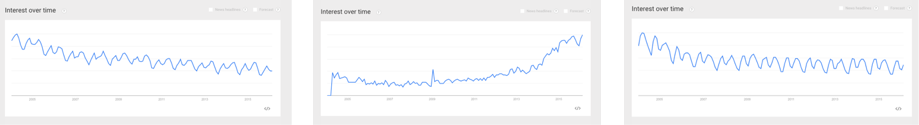
\includegraphics[width=12.76in]{images/googletrends}

\begin{enumerate}
\def\labelenumi{\arabic{enumi}.}
\setcounter{enumi}{2}
\item
  R is incredibly versatile. You can use R to do everything from
  calculating simple summary statistics, to performing complex
  simulations to creating gorgeous plots like the chord diagram on the
  right. If you can imagine an analytical task, you can almost certainly
  implement it in R.
\item
  Using RStudio, a program to help you write R code, You can easily and
  seamlessly combine R code, analyses, plots, and written text into
  elegant documents all in one place using Sweave (R and Latex) or
  RMarkdown. In fact, I translated this entire book (the text,
  formatting, plots, code\ldots{}yes, everything) in RStudio using
  Sweave. With RStudio and Sweave, instead of trying to manage two or
  three programs, say Excel, Word and (sigh) SPSS, where you find
  yourself spending half your time copying, pasting and formatting data,
  images and test, you can do everything in one place so nothing gets
  misread, mistyped, or forgotten.
\end{enumerate}

\begin{Shaded}
\begin{Highlighting}[]
\NormalTok{circlize}\OperatorTok{::}\KeywordTok{chordDiagram}\NormalTok{(}\KeywordTok{matrix}\NormalTok{(}\KeywordTok{sample}\NormalTok{(}\DecValTok{10}\NormalTok{), }
                              \DataTypeTok{nrow =} \DecValTok{2}\NormalTok{, }\DataTypeTok{ncol =} \DecValTok{5}\NormalTok{))}
\end{Highlighting}
\end{Shaded}

\begin{figure}
\centering
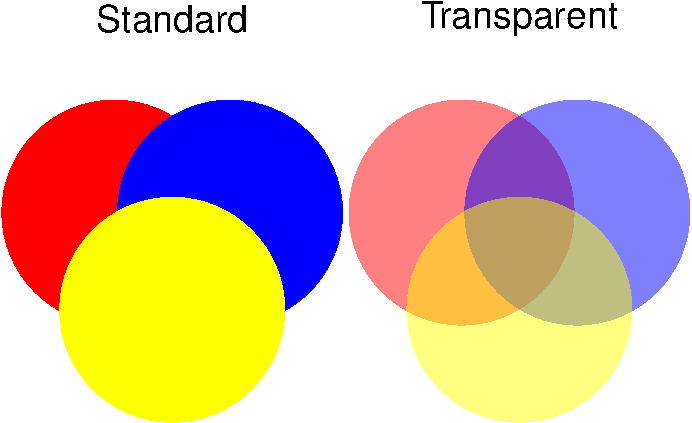
\includegraphics{YaRrr_files/figure-latex/unnamed-chunk-3-1.pdf}
\caption{\label{fig:unnamed-chunk-3}A super cool chord diagram from the
circlize package}
\end{figure}

\begin{enumerate}
\def\labelenumi{\arabic{enumi}.}
\setcounter{enumi}{4}
\item
  Analyses conducted in R are transparent, easily shareable, and
  reproducible. If you ask an SPSS user how they conducted a specific
  analyses, they will either A) Not remember, B) Try (nervously) to
  construct an analysis procedure on the spot that makes sense - which
  may or may not correspond to what they actually did months or years
  ago, or C) Ask you what you are doing in their house. I used to
  primarily use SPSS, so I speak from experience on this. If you ask an
  R user (who uses good programming techniques!) how they conducted an
  analysis, they should always be able to show you the exact code they
  used. Of course, this doesn't mean that they used the appropriate
  analysis or interpreted it correctly, but with all the original code,
  any problems should be completely transparent!
\item
  And most importantly of all, R is the programming language of choice
  for pirates.
\end{enumerate}

\hypertarget{rrelationship}{\section{Why R is like a
relationship\ldots{}}\label{rrelationship}}

Yes, R is very much like a relationship. Like relationships, there are
two major truths to R programming:

\begin{figure}

{\centering 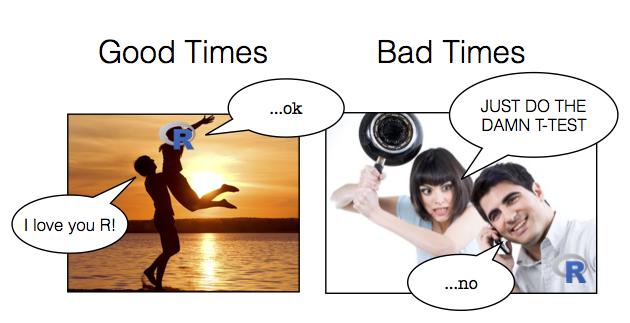
\includegraphics[width=8.75in]{images/rrelationship} 

}

\caption{Yep, R will become both your best friend and your worst nightmare. The bad times will make the good times oh so much sweeter.}\label{fig:unnamed-chunk-4}
\end{figure}

\begin{enumerate}
\def\labelenumi{\arabic{enumi}.}
\item
  There is nothing more \emph{frustrating} than when your code does
  \emph{not} work
\item
  There is nothing more \emph{satisfying} than when your code
  \emph{does} work!
\end{enumerate}

Anything worth doing, from losing weight to getting a degree, takes
time. Learning R is no different. Especially if this is your first
experience programming, you are going to experience a \emph{lot} of
headaches when you get started. You will run into error after error and
pound your fists against the table screaming: ``WHY ISN'T MY CODE
WORKING?!?!? There must be something wrong with this stupid
software!!!'' You will spend hours trying to find a bug in your code,
only to find that - frustratingly enough, you had had an extra space or
missed a comma somewhere. You'll then wonder why you ever decided to
learn R when (::sigh::) SPSS was so ``nice and easy.''

\begin{figure}

{\centering 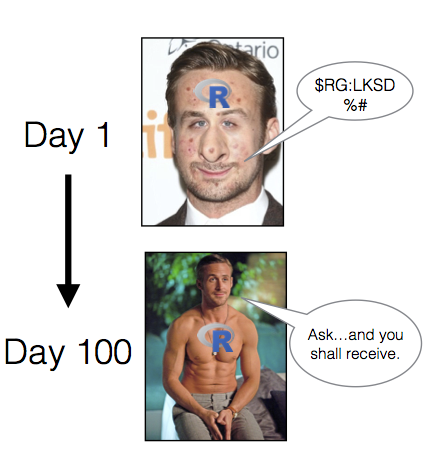
\includegraphics[width=5.99in]{images/gosling} 

}

\caption{When you first meet R, it will look so fugly that you'll wonder if this is all some kind of sick joke. But trust me, once you learn how to talk to it, and clean it up a bit, all your friends will be crazy jealous.}\label{fig:unnamed-chunk-5}
\end{figure}

\textbf{Fun Fact!} SPSS stands for ``Shitty Piece of Shitty Shit''. True
story.

This is perfectly normal! Don't get discouraged and DON'T GO BACK TO
SPSS! That would be quitting on exercise altogether because you had a
tough workout.

Trust me, as you gain more programming experience, you'll experience
fewer and fewer bugs (though they'll never go away completely). Once you
get over the initial barriers, you'll find yourself conducting analyses
much, much faster than you ever did before.

\section{R resources}\label{r-resources}

\subsection{R Cheatsheets}\label{r-cheatsheets}

\begin{figure}

{\centering 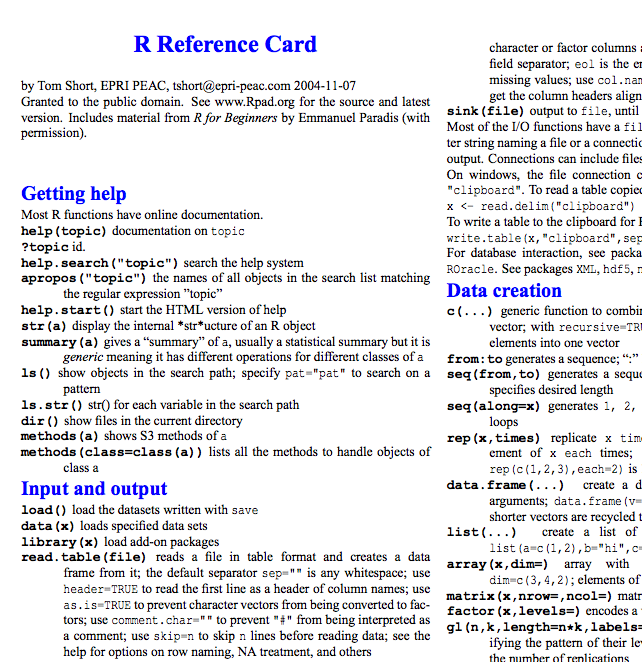
\includegraphics[width=0.75\linewidth]{images/rreferencess} 

}

\caption{The R reference card written by Tom Short is absolutely indispensable!}\label{fig:rreferencecard}
\end{figure}

Over the course of this book, you will be learning \emph{lots} of new
functions. Wouldn't it be nice if someone created a Cheatsheet /
Dictionary of many common R functions? Yes it would, and thankfully
several friendly R programmers have done just that. Below is a table of
some of them that I recommend. I highly encourage you to print these out
and start highlighting functions as you learn them!

\begin{longtable}[]{@{}ll@{}}
\toprule
\begin{minipage}[b]{0.39\columnwidth}\raggedright\strut
CheatSheet\strut
\end{minipage} & \begin{minipage}[b]{0.13\columnwidth}\raggedright\strut
Link\strut
\end{minipage}\tabularnewline
\midrule
\endhead
\begin{minipage}[t]{0.39\columnwidth}\raggedright\strut
R Basics by Tom Short\strut
\end{minipage} & \begin{minipage}[t]{0.13\columnwidth}\raggedright\strut
\url{https://cran.r-project.org/doc/contrib/Short-refcard.pdf}\strut
\end{minipage}\tabularnewline
\begin{minipage}[t]{0.39\columnwidth}\raggedright\strut
R Basics by Mhairi McNeill\strut
\end{minipage} & \begin{minipage}[t]{0.13\columnwidth}\raggedright\strut
\url{http://github.com/rstudio/cheatsheets/raw/master/source/pdfs/base-r.pdf}\strut
\end{minipage}\tabularnewline
\begin{minipage}[t]{0.39\columnwidth}\raggedright\strut
Advanced R by Arianne Colton and Sean Chen\strut
\end{minipage} & \begin{minipage}[t]{0.13\columnwidth}\raggedright\strut
\href{https://www.rstudio.com/wp-content/uploads/2016/02/advancedR.pdf}{hhttps://www.rstudio.com/wp-content/uploads/2016/02/advancedR.pdf}\strut
\end{minipage}\tabularnewline
\begin{minipage}[t]{0.39\columnwidth}\raggedright\strut
Plotting\strut
\end{minipage} & \begin{minipage}[t]{0.13\columnwidth}\raggedright\strut
\url{https://www.rstudio.com/wp-content/uploads/2016/10/how-big-is-your-graph.pdf}\strut
\end{minipage}\tabularnewline
\bottomrule
\end{longtable}

\subsection{Getting R help and inspiration
online}\label{getting-r-help-and-inspiration-online}

Here are some great resources for R help and inspiration:

\begin{longtable}[]{@{}ll@{}}
\toprule
\begin{minipage}[b]{0.39\columnwidth}\raggedright\strut
Site\strut
\end{minipage} & \begin{minipage}[b]{0.48\columnwidth}\raggedright\strut
Description\strut
\end{minipage}\tabularnewline
\midrule
\endhead
\begin{minipage}[t]{0.39\columnwidth}\raggedright\strut
\href{http://www.google.com}{www.google.com}\strut
\end{minipage} & \begin{minipage}[t]{0.48\columnwidth}\raggedright\strut
If you haven't heard of it, Google is this amazing site that gives you
access to all R knowledge that has ever existed. Just ask it an R
question and 99.9\% of the time it will give you the answer!\strut
\end{minipage}\tabularnewline
\begin{minipage}[t]{0.39\columnwidth}\raggedright\strut
\href{http://www.r-bloggers.com}{www.r-bloggers.com}\strut
\end{minipage} & \begin{minipage}[t]{0.48\columnwidth}\raggedright\strut
R bloggers is my go-to place to discover the latest and greatest with
R.\strut
\end{minipage}\tabularnewline
\begin{minipage}[t]{0.39\columnwidth}\raggedright\strut
\href{http://blog.revolutionanalytics.com}{blog.revolutionanalytics.com}\strut
\end{minipage} & \begin{minipage}[t]{0.48\columnwidth}\raggedright\strut
Revolution analytics always has great R related material.\strut
\end{minipage}\tabularnewline
\begin{minipage}[t]{0.39\columnwidth}\raggedright\strut
\href{http://www.kaggle.com}{www.kaggle.com}\strut
\end{minipage} & \begin{minipage}[t]{0.48\columnwidth}\raggedright\strut
Kaggle is a really cool website that posts data analysis challenges that
anyone can try to solve. It also contains a wide range of real-world
datasets and tutorials.\strut
\end{minipage}\tabularnewline
\bottomrule
\end{longtable}

\subsection{Other R books}\label{other-r-books}

There are many, many excellent (non-pirate) books on R, some of which
are available online for free. Here are some that I highly recommend:

\begin{longtable}[]{@{}ll@{}}
\toprule
\begin{minipage}[b]{0.39\columnwidth}\raggedright\strut
Book\strut
\end{minipage} & \begin{minipage}[b]{0.48\columnwidth}\raggedright\strut
Description\strut
\end{minipage}\tabularnewline
\midrule
\endhead
\begin{minipage}[t]{0.39\columnwidth}\raggedright\strut
\href{http://r4ds.had.co.nz/}{R for Data Science by Garrett Grolemund
and Hadley Wickham}\strut
\end{minipage} & \begin{minipage}[t]{0.48\columnwidth}\raggedright\strut
The best book to learn the latest tools for elegantly doing data
science.\strut
\end{minipage}\tabularnewline
\begin{minipage}[t]{0.39\columnwidth}\raggedright\strut
\href{https://www.amazon.com/R-Book-Michael-J-Crawley/dp/0470973927/ref=sr_1_1?ie=UTF8\&qid=1487759048\&sr=8-1\&keywords=the+r+book}{The
R Book by Michael Crawley}\strut
\end{minipage} & \begin{minipage}[t]{0.48\columnwidth}\raggedright\strut
As close to an R bible as you can get.\strut
\end{minipage}\tabularnewline
\begin{minipage}[t]{0.39\columnwidth}\raggedright\strut
\href{http://adv-r.had.co.nz/}{Advanced R by Hadley Wickham}\strut
\end{minipage} & \begin{minipage}[t]{0.48\columnwidth}\raggedright\strut
A truly advanced book for expert R users, especially those with a
programming background. Hadley Wickham is \emph{the} R guru.\strut
\end{minipage}\tabularnewline
\begin{minipage}[t]{0.39\columnwidth}\raggedright\strut
\href{https://www.amazon.com/Discovering-Statistics-Using-Andy-Field/dp/1446200469/ref=sr_1_2?ie=UTF8\&qid=1487759316\&sr=8-2\&keywords=statistics+with+r}{Discovering
Statistics with R by Field, Miles and Field}\strut
\end{minipage} & \begin{minipage}[t]{0.48\columnwidth}\raggedright\strut
A classic text focusing on the theory and practice of statistical
analysis with R\strut
\end{minipage}\tabularnewline
\begin{minipage}[t]{0.39\columnwidth}\raggedright\strut
\href{https://www.amazon.com/Applied-Predictive-Modeling-Max-Kuhn/dp/1461468485/ref=sr_1_1?ie=UTF8\&qid=1487759459\&sr=8-1\&keywords=applied+predictive+modeling}{Applied
Predictive Modeling by Kuhn and Johnson}\strut
\end{minipage} & \begin{minipage}[t]{0.48\columnwidth}\raggedright\strut
A great text specializing in statistical learning aka predictive
modeling aka machine learning with R.\strut
\end{minipage}\tabularnewline
\bottomrule
\end{longtable}

\section{Who am I?}\label{who-am-i}

\begin{figure}

{\centering 
\includegraphics[width=7.49in]{images/beer} 

}

\caption{Like a pirate, I work best with a mug of beer within arms' reach.}\label{fig:unnamed-chunk-6}
\end{figure}

My name is Nathaniel -- not Nathan\ldots{}not Nate\ldots{}and
\emph{definitely} not Nat. I am a psychologist with a background in
statistics and judgment and decision making. You can find my R (and
non-R) related musings at \url{http://ndphillips.github.io}

\subsection{Acknowledgements}\label{acknowledgements}

I am deeply indebted to many people for either directly or indirectly
helping me make this book happen. I would especially like to thank
\href{https://www.grinnell.edu/users/mooret}{Captain Thomas Moore} and
\href{http://www.math.ohiou.edu/people/directory/linwei}{Captain Wei
Linn} for my early training in both statistics and R,
\href{https://www.spds.uni-konstanz.de/hans-neth}{Captain Hansjoerg
Neth} for teaching me LaTeX and ultimately inspiring me to write (I mean
translate) this book, and
\href{https://psycho.unibas.ch/fakultaet/personen/profil/person/wulff/}{Captain
Dirk Wulff} for teaching me almost everything I know about R. If I
hadn't been lucky enough to meet just one of these people, this book
would not exist.

\section{Please Contribute!}\label{please-contribute}

I am grateful for comments, questions, bug reports, and requests to
future editions of the book! If there's anything you'd like to add or
share, please contact me via email at
\href{mailto:yarrr.book@gmail.com}{\nolinkurl{yarrr.book@gmail.com}}, or
if you are familiar with GitHub, post an issue at
\url{https://github.com/ndphillips/ThePiratesGuideToR/issues}.
Contributers will be added to the R pirate

\chapter{Getting Started}\label{started}

\section{Installing Base-R and
RStudio}\label{installing-base-r-and-rstudio}

To use R, we'll need to download two software packages: \textbf{Base-R},
and \textbf{RStudio}. Base-R is the basic software which contains the R
programming language. RStudio is software that makes R programming
easier. Of course, they are totally free and open source.

\subsection{Check for version updates}\label{check-for-version-updates}

R and RStudio have been around for several years -- however, they are
\emph{constantly} being updated with new features and bug-fixes. At the
time that I am writing this sentence (09:48, Thursday, 23 February,
2017), the latest version of Base-R is 3.3.2 ``Sincere Pumpkin Patch''
(the versions all have funny names) which was released on 31 October,
2016, and the latest version of RStudio is 1.0.136 released on 21
December, 2016. If you have a (much) older version of R or RStudio
currently installed on your computer, then you should update both R and
RStudio to the newest version(s) by installing them again from scratch.
If you don't, then some of the code and packages in this book might not
work.

\begin{figure}

{\centering \includegraphics[width=0.4\linewidth]{images/rlogo} 

}

\end{figure}

To install Base-R, click on one of the following links and follow the
instructions.

\begin{longtable}[]{@{}ll@{}}
\toprule
Operating System & Link\tabularnewline
\midrule
\endhead
Windows &
\url{http://cran.r-project.org/bin/windows/base/}\tabularnewline
Mac & \url{http://cran.r-project.org/bin/macosx/}\tabularnewline
\bottomrule
\end{longtable}

Once you've installed base-R on your computer, try opening it. When you
do you should see a screen like the one in Figure \ref{fig:rscreenshot}
(this is the Mac version). As you can see, base R is very much
bare-bones software. It's kind of the equivalent of a simple text editor
that comes with your computer.

\textbackslash{}begin\{figure\}

\{\centering 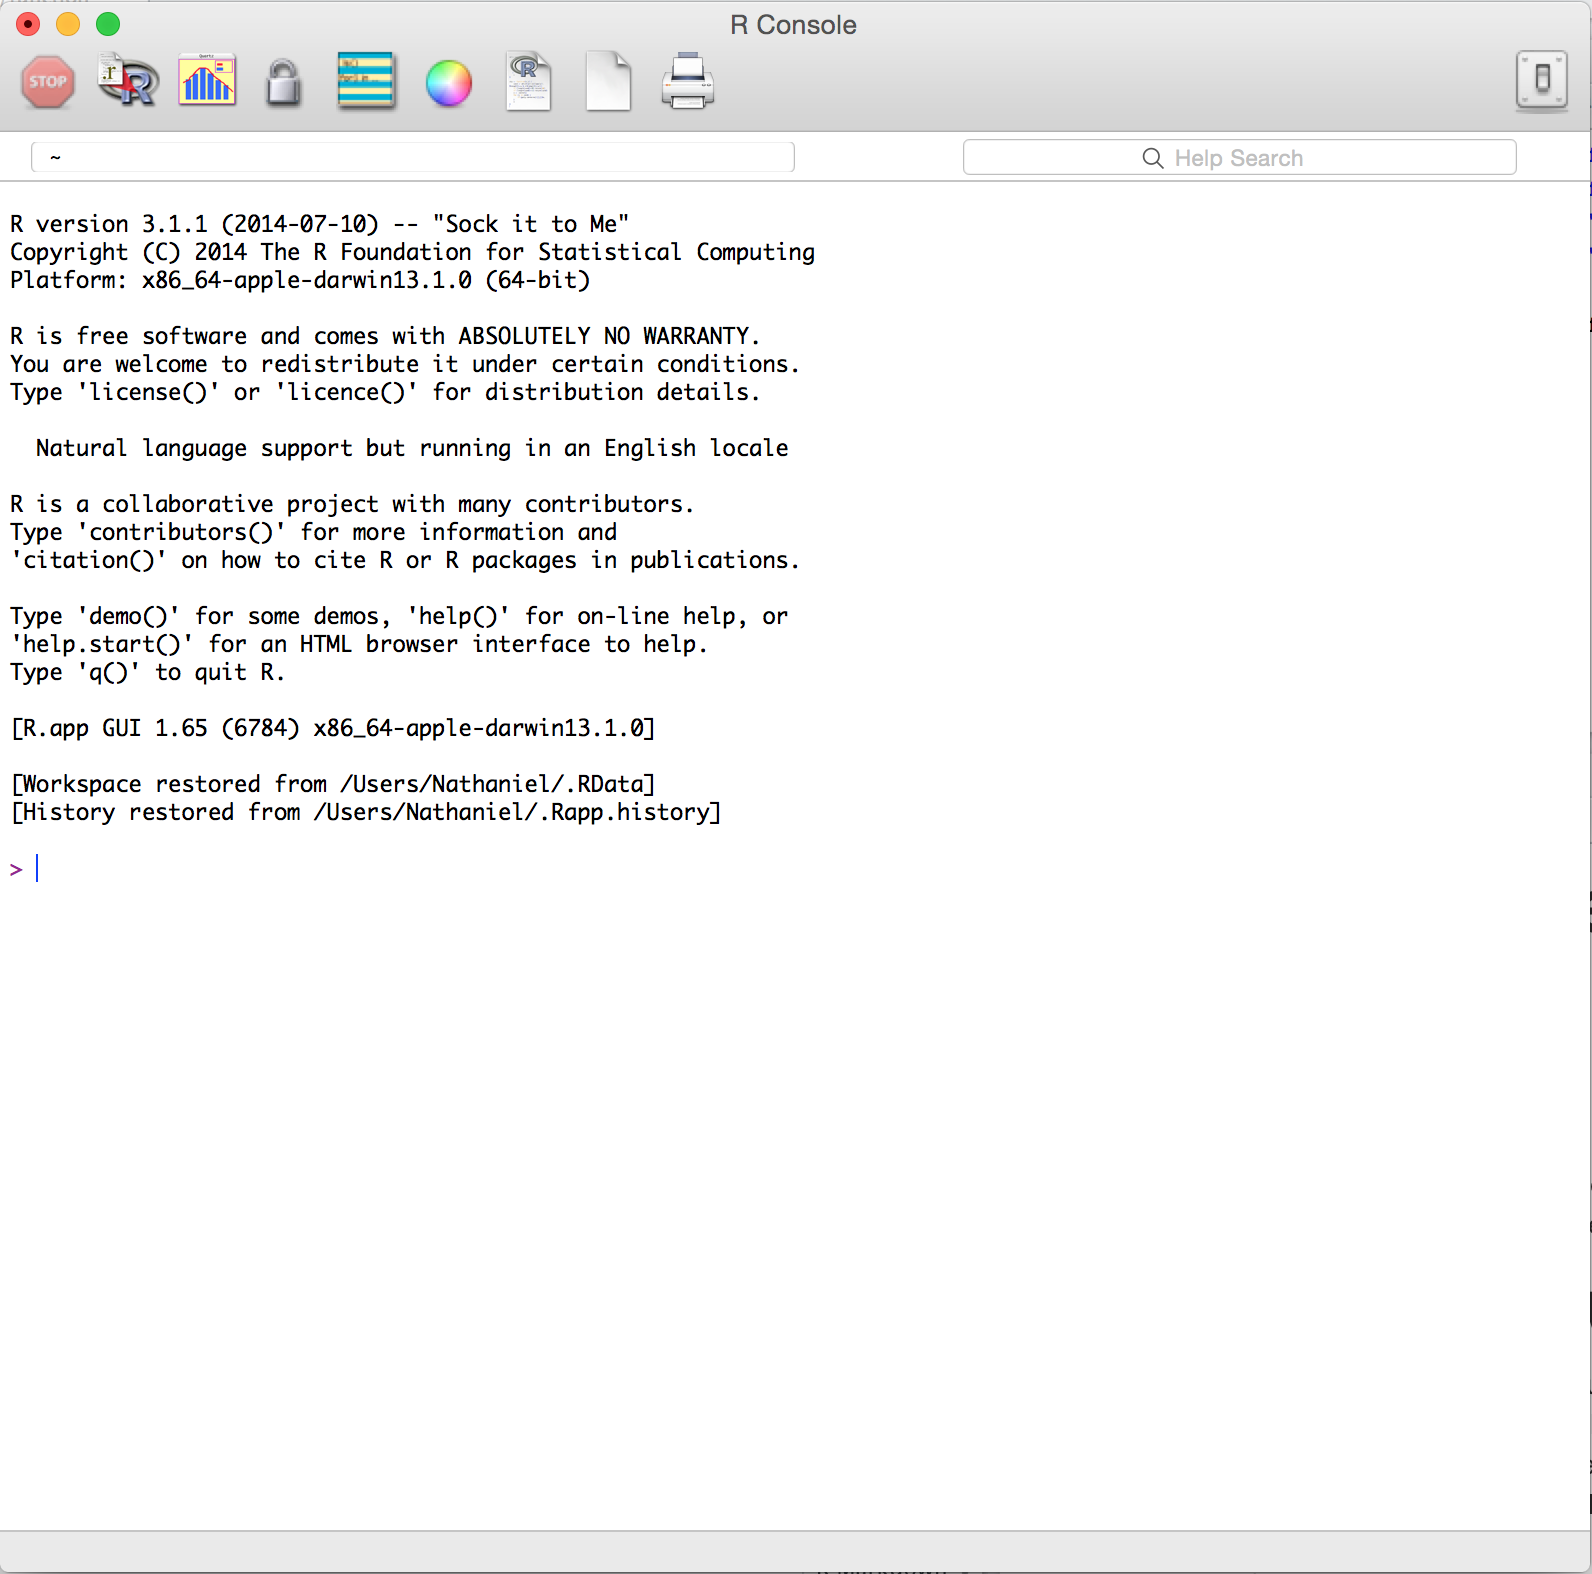
\includegraphics[width=0.75\linewidth]{images/RScreenshot}

\}

\textbackslash{}caption\{\{Here is how the base R application looks.
While you can use the base R application alone, most people I know use
RStudio -- software that helps you to write and use R code more
efficiently!\}\label{fig:rscreenshot} \textbackslash{}end\{figure\}

\begin{figure}

{\centering 
\includegraphics[width=0.4\linewidth]{images/RStudio} 

}

\end{figure}

While you can do pretty much everything you want within base-R, you'll
find that most people these days do their R programming in an
application called RStudio. RStudio is a graphical user interface
(GUI)-like interface for R that makes programming in R a bit easier. In
fact, once you've installed RStudio, you'll likely never need to open
the base R application again. To download and install RStudio (around
40mb), go to one of the links above and follow the instructions.

\begin{longtable}[]{@{}ll@{}}
\toprule
Operating System & Link\tabularnewline
\midrule
\endhead
All &
\url{http://www.rstudio.com/products/rstudio/download/}\tabularnewline
\bottomrule
\end{longtable}

Let's go ahead and boot up RStudio and see how she looks!

\section{The four RStudio Windows}\label{the-four-rstudio-windows}

When you open RStudio, you'll see the following four windows (also
called panes) shown in in Figure \ref{fig:rstudiowindows}. However, your
windows might be in a different order that those in Figure
\ref{fig:rstudiowindows}. If you'd like, you can change the order of the
windows under RStudio preferences. You can also change their shape by
either clicking the minimize or maximize buttons on the top right of
each panel, or by clicking and dragging the middle of the borders of the
windows.

\begin{figure}

{\centering 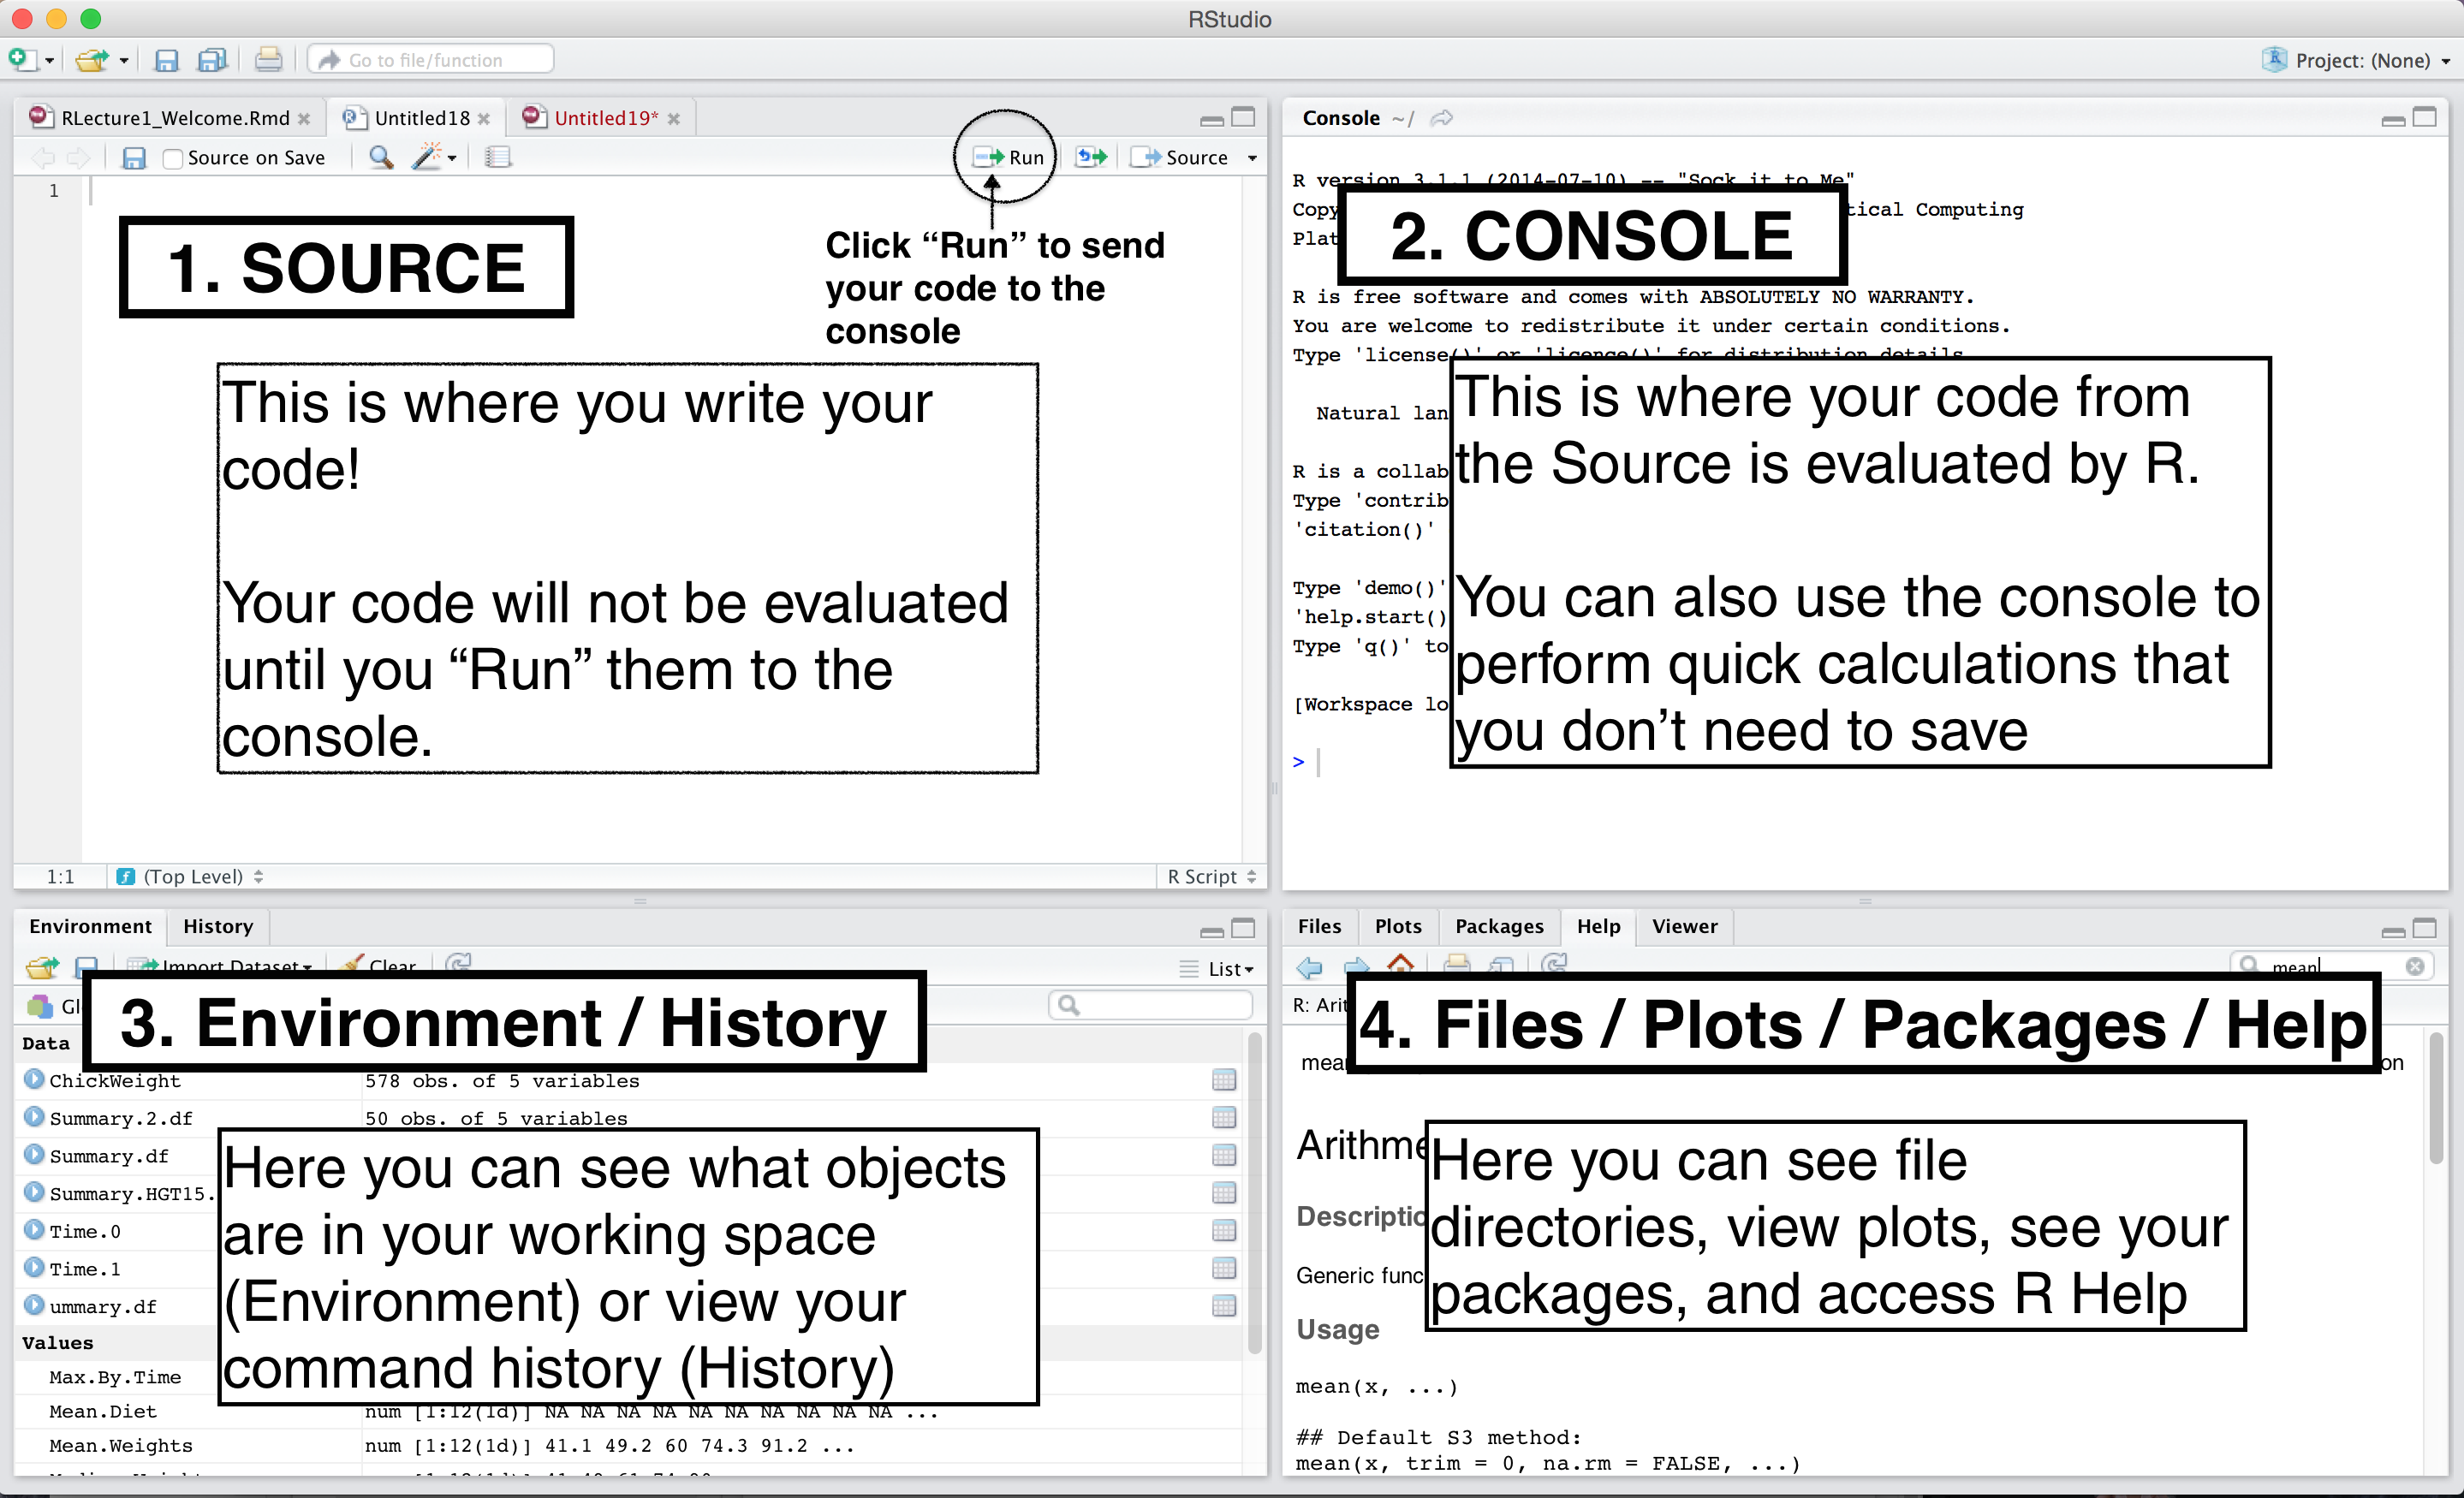
\includegraphics[width=1\linewidth]{images/RStudio_Screenshot_Labels} 

}

\caption{The four panes of RStudio.}\label{fig:rstudiowindows}
\end{figure}

Now, let's see what each window does in detail.

\subsection{Source - Your notepad for
code}\label{source---your-notepad-for-code}

\begin{figure}

{\centering 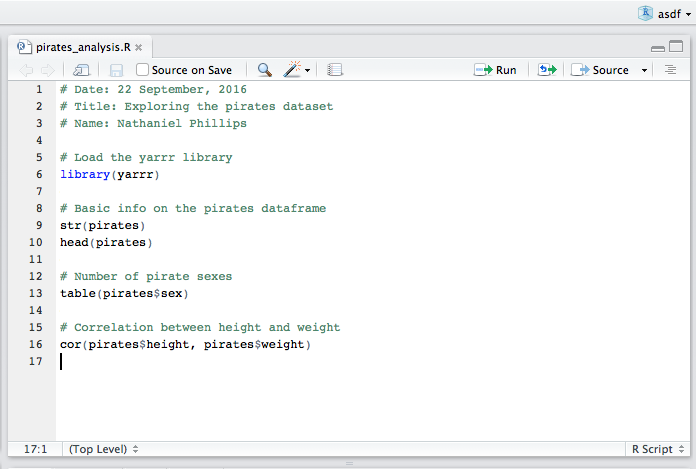
\includegraphics[width=1\linewidth]{images/piratesanalysisss} 

}

\caption{The Source contains all of your individual R scripts. The code won't be evaluated until you send it to the Console.}\label{fig:sourcewindow}
\end{figure}

The source pane is where you create and edit ``R Scripts" - your
collections of code. Don't worry, R scripts are just text files with the
``.R'' extension. When you open RStudio, it will automatically start a
new Untitled script. Before you start typing in an untitled R script,
you should always save the file under a new file name (like,
``2015PirateSurvey.R''). That way, if something on your computer crashes
while you're working, R will have your code waiting for you when you
re-open RStudio.

You'll notice that when you're typing code in a script in the Source
panel, R won't actually evaluate the code as you type. To have R
actually evaluate your code, you need to first `send' the code to the
Console (we'll talk about this in the next section).

There are many ways to send your code from the Source to the console.
The slowest way is to copy and paste. A faster way is to highlight the
code you wish to evaluate and clicking on the ``Run'' button on the top
right of the Source. Alternatively, you can use the hot-key ``Command +
Return'' on Mac, or ``Control + Enter'' on PC to send all highlighted
code to the console.

\subsection{Console: R's Heart}\label{console-rs-heart}

\begin{figure}
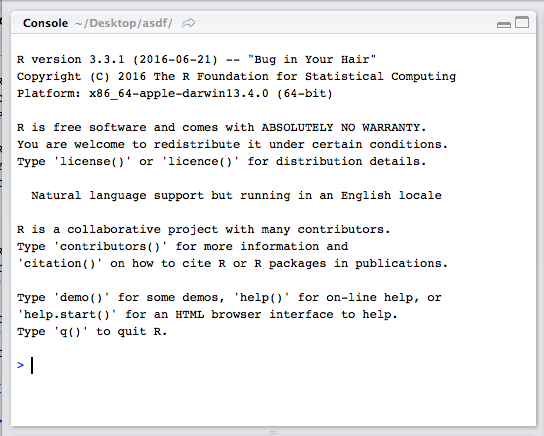
\includegraphics[width=0.75\linewidth]{images/consoless} \caption{The console the calculation heart of R. All of your code will (eventually) go through here.}\label{fig:consolewindow}
\end{figure}

The console is the heart of R. Here is where R actually evaluates code.
At the beginning of the console you'll see the character \texttt{>}.
This is a prompt that tells you that R is ready for new code. You can
type code directly into the console after the \texttt{>} prompt and get
an immediate response. For example, if you type 1+1 into the console and
press enter, you'll see that R immediately gives an output of 2.

\begin{Shaded}
\begin{Highlighting}[]
\DecValTok{1}\OperatorTok{+}\DecValTok{1}
\NormalTok{## [1] 2}
\end{Highlighting}
\end{Shaded}

Try calculating 1+1 by typing the code directly into the console - then
press Enter. You should see the result {[}1{]} 2. Don't worry about the
{[}1{]} for now, we'll get to that later. For now, we're happy if we
just see the 2. Then, type the same code into the Source, and then send
the code to the Console by highlighting the code and clicking the ``Run"
button on the top right hand corner of the Source window. Alternatively,
you can use the hot-key ``Command + Return'' on Mac or ``Control +
Enter'' on Windows.

\textbf{Tip}: Try to write most of your code in a document in the
Source. Only type directly into the Console to de-bug or do quick
analyses.

So as you can see, you can execute code either by running it from the
Source or by typing it directly into the Console. However, 99\% most of
the time, you should be using the Source rather than the Console. The
reason for this is straightforward: If you type code into the console,
it won't be saved (though you can look back on your command History).
And if you make a mistake in typing code into the console, you'd have to
re-type everything all over again. Instead, it's better to write all
your code in the Source. When you are ready to execute some code, you
can then send ``Run'' it to the console.

\subsection{Environment / History}\label{environment-history}

\begin{figure}
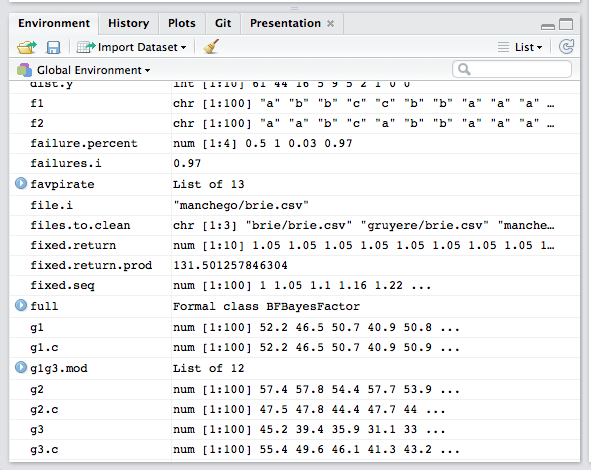
\includegraphics[width=0.75\linewidth]{images/environmentss} \caption{The environment panel shows you all the objects you have defined in your current workspace. You'll learn more about workspaces in Chapter 7.}\label{fig:environment}
\end{figure}

The Environment tab of this panel shows you the names of all the data
objects (like vectors, matrices, and dataframes) that you've defined in
your current R session. You can also see information like the number of
observations and rows in data objects. The tab also has a few clickable
actions like ``Import Dataset" which will open a graphical user
interface (GUI) for important data into R. However, I almost never look
at this menu.

The History tab of this panel simply shows you a history of all the code
you've previously evaluated in the Console. To be honest, I never look
at this. In fact, I didn't realize it was even there until I started
writing this tutorial.

As you get more comfortable with R, you might find the Environment /
History panel useful. But for now you can just ignore it. If you want to
declutter your screen, you can even just minimize the window by clicking
the minimize button on the top right of the panel.

\subsection{Files / Plots / Packages /
Help}\label{files-plots-packages-help}

The Files / Plots / Packages / Help panel shows you lots of helpful
information. Let's go through each tab in detail:

\begin{enumerate}
\def\labelenumi{\arabic{enumi}.}
\item
  Files - The files panel gives you access to the file directory on your
  hard drive. One nice feature of the ``Files'' panel is that you can
  use it to set your working directory - once you navigate to a folder
  you want to read and save files to, click ``More'' and then ``Set As
  Working Directory.'' We'll talk about working directories in more
  detail soon.
\item
  Plots - The Plots panel (no big surprise), shows all your plots. There
  are buttons for opening the plot in a separate window and exporting
  the plot as a pdf or jpeg (though you can also do this with code using
  the \texttt{pdf()} or \texttt{jpeg()} functions.)
\end{enumerate}

Let's see how plots are displayed in the Plots panel. Run the code on
the right to display a histogram of the weights of chickens stored in
the \texttt{ChickWeight} dataset. When you do, you should see a plot
similar to the one in Figure \ref{fig:plotpanel} show up in the Plots
panel.

\begin{Shaded}
\begin{Highlighting}[]
\KeywordTok{hist}\NormalTok{(}\DataTypeTok{x =}\NormalTok{ ChickWeight}\OperatorTok{$}\NormalTok{weight,}
     \DataTypeTok{main =} \StringTok{"Chicken Weights"}\NormalTok{,}
     \DataTypeTok{xlab =} \StringTok{"Weight"}\NormalTok{,}
     \DataTypeTok{col =} \StringTok{"skyblue"}\NormalTok{,}
     \DataTypeTok{border =} \StringTok{"white"}\NormalTok{)}
\end{Highlighting}
\end{Shaded}

\begin{figure}
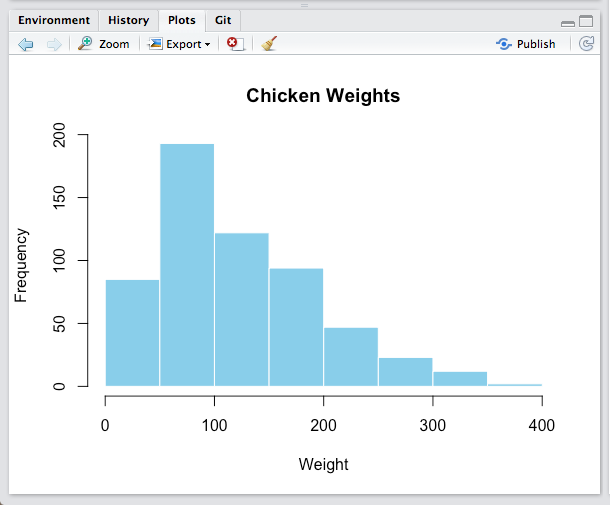
\includegraphics[width=0.75\linewidth]{images/plotpanelss} \caption{The plot panel contains all of your plots, like this histogram of the distribution of chicken weights.}\label{fig:plotpanel}
\end{figure}

\begin{enumerate}
\def\labelenumi{\arabic{enumi}.}
\setcounter{enumi}{2}
\item
  Packages - Shows a list of all the R packages installed on your
  harddrive and indicates whether or not they are currently loaded.
  Packages that are loaded in the current session are checked while
  those that are installed but not yet loaded are unchecked. We'll
  discuss packages in more detail in the next section.
\item
  Help - Help menu for R functions. You can either type the name of a
  function in the search window, or use the code \texttt{?function.name}
  to search for a function with the name \texttt{function.name}
\end{enumerate}

\begin{Shaded}
\begin{Highlighting}[]
\NormalTok{?hist   }\CommentTok{# How does the histogram function work?}
\NormalTok{?t.test }\CommentTok{# What about a t-test?}
\end{Highlighting}
\end{Shaded}

\section{Packages}\label{packages}

When you download and install R for the first time, you are installing
the Base R software. Base R will contain most of the functions you'll
use on a daily basis like \texttt{mean()} and \texttt{hist()}. However,
only functions written by the original authors of the R language will
appear here. If you want to access data and code written by other
people, you'll need to install it as a \emph{package}. An R package is
simply a bunch of data, from functions, to help menus, to vignettes
(examples), stored in one neat package.

\begin{figure}

{\centering 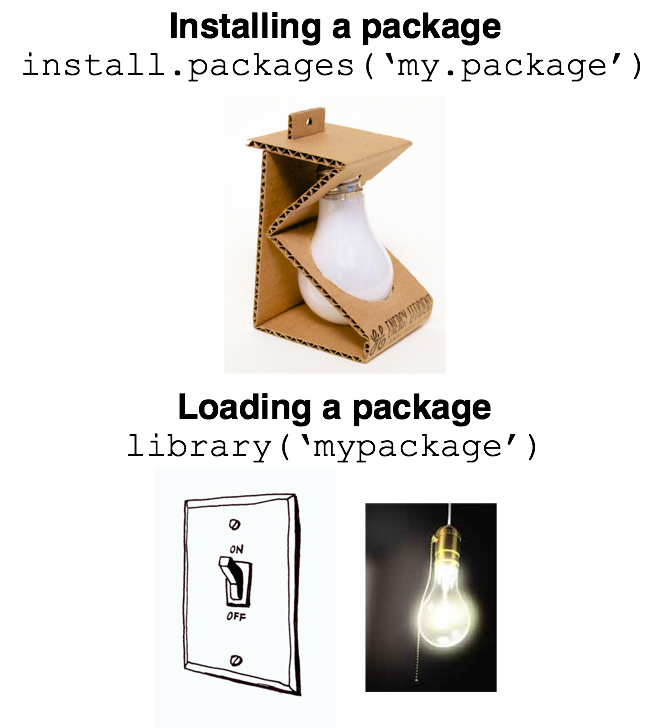
\includegraphics[width=0.5\linewidth]{images/packagebulb} 

}

\caption{An R package is light a lightbulb. First you need to order it with install.packages(). Then, every time you want to use it, you need to turn it on with library()}\label{fig:package}
\end{figure}

A package is like a light bulb. In order to use it, you first need to
order it to your house (i.e.; your computer) by \emph{installing} it.
Once you've installed a package, you never need to install it again.
However, every time you want to actually use the package, you need to
turn it on by \emph{loading} it. Here's how to do it.

\subsection{Installing a new package}\label{installing-a-new-package}

Installing a package simply means downloading the package code onto your
personal computer. There are two main ways to install new packages. The
first, and most common, method is to download them from the
Comprehensive R Archive Network (CRAN). CRAN is the central repository
for R packages. To install a new R package from CRAN, you can simply run
the code \texttt{install.packages("name")}, where ``name'' is the name
of the package. For example, to download the \texttt{yarrr} package,
which contains several data sets and functions we will use in this book,
you should run the following:

\begin{figure}

{\centering 
\includegraphics[width=0.5\linewidth]{images/cran} 

}

\caption{CRAN (Comprehensive R Archive Network) is the main source of R packages}\label{fig:cran}
\end{figure}

\begin{Shaded}
\begin{Highlighting}[]
\CommentTok{# Install the yarrr package from CRAN}
\CommentTok{#   You only need to install a package once!}
\KeywordTok{install.packages}\NormalTok{(}\StringTok{"yarrr"}\NormalTok{)}
\end{Highlighting}
\end{Shaded}

When you run \texttt{install.packages("name")} R will download the
package from CRAN. If everything works, you should see some information
about where the package is being downloaded from, in addition to a
progress bar.

\begin{figure}

{\centering 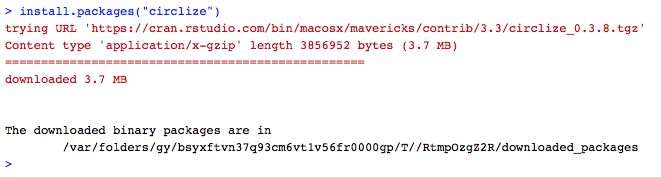
\includegraphics[width=0.75\linewidth]{images/installingpackages} 

}

\caption{When you install a new package, you'll see some random text like this you the download progress. You don't need to memorize this.}\label{fig:installingpackages}
\end{figure}

Like ordering a light bulb, once you've installed a package on your
computer you never need to install it again (unless you want to try to
install a new version of the package). However, every time you want to
use it, you need to turn it on by loading it.

\subsection{Loading a package}\label{loading-a-package}

Once you've installed a package, it's on your computer. However, just
because it's on your computer doesn't mean R is ready to use it. If you
want to use something, like a function or dataset, from a package you
\emph{always} need to \emph{load} the package in your R session first.
Just like a light bulb, you need to turn it on to use it!

To load a package, you use the \texttt{library()} function. For example,
now that we've installed the \texttt{yarrr} package, we can load it with
\texttt{library("yarrr")}:

\begin{Shaded}
\begin{Highlighting}[]
\CommentTok{# Load the yarrr package so I can use it!}
\CommentTok{#   You have to load a package in every new R session!}
\KeywordTok{library}\NormalTok{(}\StringTok{"yarrr"}\NormalTok{)}
\end{Highlighting}
\end{Shaded}

Now that you've loaded the \texttt{yarrr} package, you can use any of
its functions! One of the coolest functions in this package is called
\texttt{pirateplot()}. Rather than telling you what a pirateplot is,
let's just make one. Run the following code chunk to make your own
pirateplot. Don't worry about the specifics of the code below, you'll
learn more about how all this works later. For now, just run the code
and marvel at your pirateplot.

\begin{Shaded}
\begin{Highlighting}[]
\CommentTok{# Make a pirateplot using the pirateplot() function}
\CommentTok{#  from the yarrr package!}

\KeywordTok{pirateplot}\NormalTok{(}\DataTypeTok{formula =}\NormalTok{ weight }\OperatorTok{~}\StringTok{ }\NormalTok{Time, }
           \DataTypeTok{data =}\NormalTok{ ChickWeight,}
           \DataTypeTok{pal =} \StringTok{"xmen"}\NormalTok{)}
\end{Highlighting}
\end{Shaded}

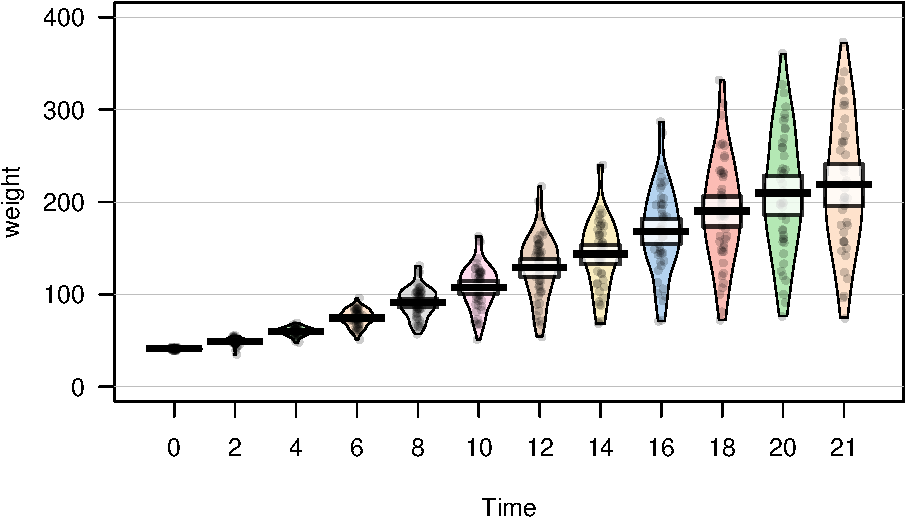
\includegraphics{YaRrr_files/figure-latex/unnamed-chunk-15-1.pdf}

There is one way in R to temporarily load a package without using the
\texttt{library()} function. To do this, you can simply use the notation
\texttt{package::function} notation. This notation simply tells R to
load the package just for this one chunk of code. For example, I could
use the \texttt{pirateplot} function from \texttt{yarrr} package as
follows:

\begin{Shaded}
\begin{Highlighting}[]
\CommentTok{# Use the pirateplot() function without loading the yarrr package first}
\NormalTok{yarrr}\OperatorTok{::}\KeywordTok{pirateplot}\NormalTok{(}\DataTypeTok{formula =}\NormalTok{ weight }\OperatorTok{~}\StringTok{ }\NormalTok{Diet,}
                  \DataTypeTok{data =}\NormalTok{ ChickWeight)}
\end{Highlighting}
\end{Shaded}

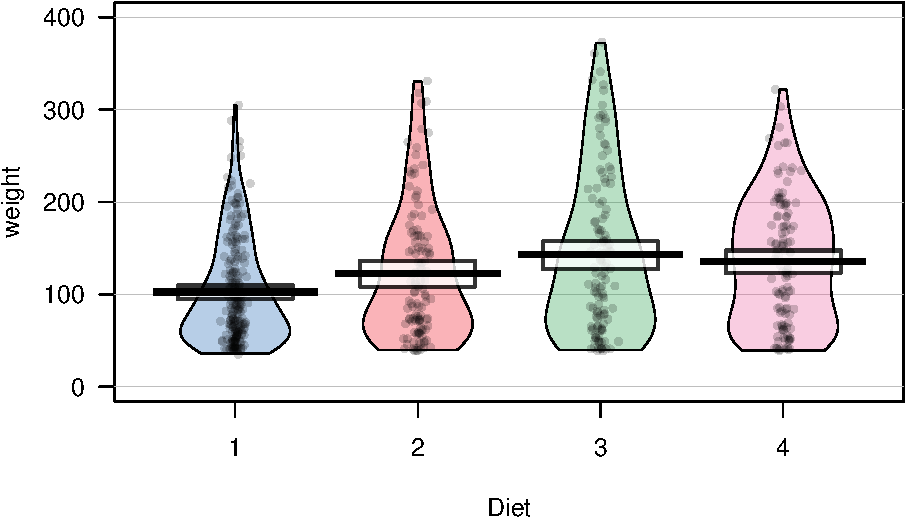
\includegraphics{YaRrr_files/figure-latex/unnamed-chunk-16-1.pdf}

Again, you can think about the \texttt{package::function} method as a
way to temporarily loading a package for a single line of code. One
benefit of using the \texttt{package::function} notation is that it's
immediately clear to anyone reading the code which package contains the
function. However, a drawback is that if you are using a function from a
package often, it forces you to constantly retype the package name. You
can use whichever method makes sense for you.

\section{Reading and writing Code}\label{reading-and-writing-code}

\subsection{Code Chunks}\label{code-chunks}

In this book, R code is (almost) always presented in a separate gray box
like this one:

\begin{Shaded}
\begin{Highlighting}[]
\CommentTok{# A code chunk}

\CommentTok{# Define a vector a as the integers from 1 to 5}
\NormalTok{a <-}\StringTok{ }\DecValTok{1}\OperatorTok{:}\DecValTok{5}

\CommentTok{# Print a}
\NormalTok{a}
\NormalTok{## [1] 1 2 3 4 5}

\CommentTok{# What is the mean of a?}
\KeywordTok{mean}\NormalTok{(a)}
\NormalTok{## [1] 3}
\end{Highlighting}
\end{Shaded}

This is called a \emph{code chunk}. You should always be able to copy
and paste code chunks directly into R. If you copy a chunk and it does
not work for you, it is most likely because the code refers to a
package, function, or object that I defined in a previous chunk. If so,
read back and look for a previous chunk that contains the missing
definition.

\subsection{Comments with \#}\label{comments-with}

Lines that begin with \# are comments. If you evaluate any code that
starts with \#, R will just ignore that line. In this book, comments
will be either be literal comments that I write directly to explain
code, or they will be \emph{output} generated automatically from R. For
example, in the code chunk below, you see lines starting with \#\#.
These are the output from the previous line(s) of code. When you run the
code yourself, you should see the same output in your \emph{console}.

\begin{Shaded}
\begin{Highlighting}[]
\CommentTok{# This is a comment I wrote}

\DecValTok{1} \OperatorTok{+}\StringTok{ }\DecValTok{2}
\NormalTok{## [1] 3}

\CommentTok{# The line above (## [1] 3) is the output from the previous code that has been 'commented out'}
\end{Highlighting}
\end{Shaded}

\subsection{Element numbers in output
{[}1{]}}\label{element-numbers-in-output-1}

The output you see will often start with one or more number(s) in
brackets such as {[}1{]}. This is just a visual way of telling you where
the numbers occur in the output. For example, in the code below, I will
print a long vector containing the multiples of 2 from 0 to 100:

\begin{Shaded}
\begin{Highlighting}[]
\KeywordTok{seq}\NormalTok{(}\DataTypeTok{from =} \DecValTok{0}\NormalTok{, }\DataTypeTok{to =} \DecValTok{100}\NormalTok{, }\DataTypeTok{by =} \DecValTok{2}\NormalTok{)}
\NormalTok{##  [1]   0   2   4   6   8  10  12  14  16  18  20  22  24  26  28  30  32}
\NormalTok{## [18]  34  36  38  40  42  44  46  48  50  52  54  56  58  60  62  64  66}
\NormalTok{## [35]  68  70  72  74  76  78  80  82  84  86  88  90  92  94  96  98 100}
\end{Highlighting}
\end{Shaded}

As you can see, the first line of the output starts with \#\# {[}1{]},
and the next two lines start with {[}18{]} and {[}35{]}. This is just
telling you that 0 is the {[}1{]}st element, 34 is the {[}18{]}th
element, and 68 is the {[}35{]}th element. Sometimes this information
will be helpful, but most of the time you can just ignore it.

\section{Debugging}\label{debugging}

When you are programming, you will always, and I do mean always, make
errors (also called bugs) in your code. You might misspell a function,
include an extra comma, or some days\ldots{}R just won't want to work
with you (again, see section \protect\hyperlink{rrelationship}{Why R is
like a Relationship}).

Debugging will always be a challenge. However, over time you'll learn
which bugs are the most common and get faster and faster at finding and
correcting them.

Here are the most common bugs you'll run into as you start your R
journey.

\subsection{R is not ready (\textgreater{})}\label{r-is-not-ready}

Another very common problem occurs when R does not seem to be responding
to your code. That is, you might run some code like \texttt{mean(x)}
expecting some output, but instead, nothing happens. This can be very
frustrating because, rather than getting an error, just nothing happens
at all. The most common reason for this is because R isn't \emph{ready}
for new code, instead, it is \emph{waiting} for you to finish code you
started earlier, but never properly finished.

Think about it this way, R can be in one of two states: it is either
\textbf{Ready} (\textgreater{}) for new code, or it is \textbf{Waiting}
(+) for you to finish old code. To see which state R is in, all you have
to do is look at the symbol on the console. The \texttt{\textgreater{}}
symbol means that R is Ready for new code -- this is usually what you
want to see. The \texttt{+} symbol means that R is Waiting for you to
(properly) finish code you started before. If you see the \texttt{+}
symbol, then no matter how much new code you write, R won't actually
evaluate it until you finish the code you started before.

Thankfully there is an easy solution to this problem (See Figure
\ref{fig:rstate}): Just hit the escape key on your keyboard. This will
cancel R's waiting state and make it Ready!

\begin{figure}

{\centering 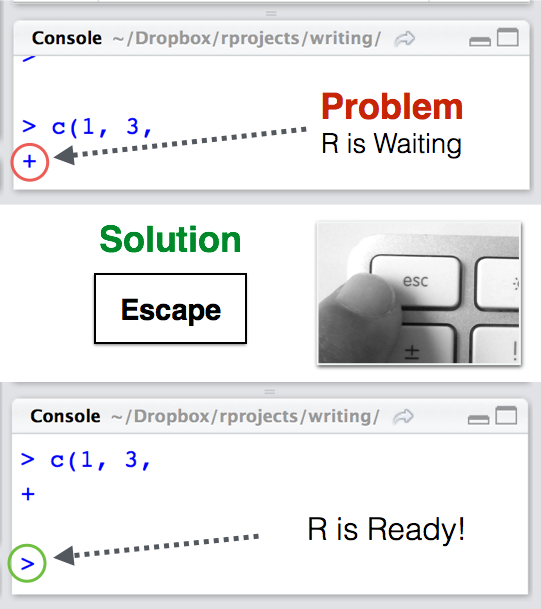
\includegraphics[width=0.5\linewidth]{images/escapesolution} 

}

\caption{To turn R from a Waiting (+) state to a Ready (>) state, just hit Escape.}\label{fig:rstate}
\end{figure}

\subsection{Misspelled object or
function}\label{misspelled-object-or-function}

If you spell an object or function incorrectly, you'll receive an error
like \texttt{Error:\ could\ not\ find\ function} or
\texttt{Error:\ object\ \textquotesingle{}x\textquotesingle{}\ not\ found}.

In the code below, I'll try to take the mean of a vector \texttt{data},
but I will misspell the function \texttt{mean()}

\begin{Shaded}
\begin{Highlighting}[]
\NormalTok{data <-}\StringTok{ }\KeywordTok{c}\NormalTok{(}\DecValTok{1}\NormalTok{, }\DecValTok{4}\NormalTok{, }\DecValTok{3}\NormalTok{, }\DecValTok{2}\NormalTok{, }\DecValTok{1}\NormalTok{)}

\CommentTok{# Misspelled function: should be mean(x), not meeen(x)}
\KeywordTok{meeen}\NormalTok{(data)}
\end{Highlighting}
\end{Shaded}

Error: could not find function ``meeen''

Now, I'll misspell the object \texttt{data} as \texttt{dta}:

\begin{Shaded}
\begin{Highlighting}[]
\CommentTok{# Misspelled object: should be data, not dta}
\KeywordTok{mean}\NormalTok{(dta)}
\end{Highlighting}
\end{Shaded}

Error: object `dta' not found

R is case-sensitive, so if you don't use the correct capitalization
you'll receive an error. In the code below, I'll use \texttt{Mean()}
instead of the correct version \texttt{mean()}

\begin{Shaded}
\begin{Highlighting}[]
\CommentTok{# Capitalization is wrong: should be mean(), not Mean()}
\KeywordTok{Mean}\NormalTok{(data)}
\end{Highlighting}
\end{Shaded}

Error: could not find function ``Mean''

Here is the correct version where both the object \texttt{data} and
function \texttt{mean()} are correctly spelled:

\begin{Shaded}
\begin{Highlighting}[]
\CommentTok{# Correct: both the object and function are correctly spelled}
\KeywordTok{mean}\NormalTok{(data)}
\NormalTok{## [1] 2.2}
\end{Highlighting}
\end{Shaded}

\subsection{Punctuation problems}\label{punctuation-problems}

Another common error is having bad coding ``punctuation''. By that, I
mean having an extra space, missing a comma, or using a comma (,)
instead of a period (.). In the code below, I'll try to create a vector
using periods instead of commas:

\begin{Shaded}
\begin{Highlighting}[]
\CommentTok{# Wrong: Using periods (.) instead of commas (,)}
\KeywordTok{mean}\NormalTok{(}\KeywordTok{c}\NormalTok{(}\DecValTok{1}\NormalTok{. }\DecValTok{4}\NormalTok{. }\DecValTok{2}\NormalTok{))}
\end{Highlighting}
\end{Shaded}

Error: unexpected numeric constant in ``mean(c(1. 4.''

Because I used periods instead of commas, I get the above error. Here is
the correct version

\begin{Shaded}
\begin{Highlighting}[]
\CommentTok{# Correct}
\KeywordTok{mean}\NormalTok{(}\KeywordTok{c}\NormalTok{(}\DecValTok{1}\NormalTok{, }\DecValTok{4}\NormalTok{, }\DecValTok{2}\NormalTok{))}
\NormalTok{## [1] 2.3}
\end{Highlighting}
\end{Shaded}

If you include an extra space in the middle of the name of an object or
function, you'll receive an error. In the code below, I'll accidentally
write \texttt{Chick\ Weight} instead of \texttt{ChickWeight}:

\begin{Shaded}
\begin{Highlighting}[]
\CommentTok{# Wrong: Extra space in the ChickWeight object name}
\KeywordTok{head}\NormalTok{(Chick Weight)}
\end{Highlighting}
\end{Shaded}

Error: unexpected symbol in ``head(Chick Weight''

Because I had an extra space in the object name, I get the above error.
Here is the correction:

\begin{Shaded}
\begin{Highlighting}[]
\CommentTok{# Correct:}
\KeywordTok{head}\NormalTok{(ChickWeight)}
\end{Highlighting}
\end{Shaded}

\chapter{Jump In!}\label{jumpin}

\begin{figure}

{\centering 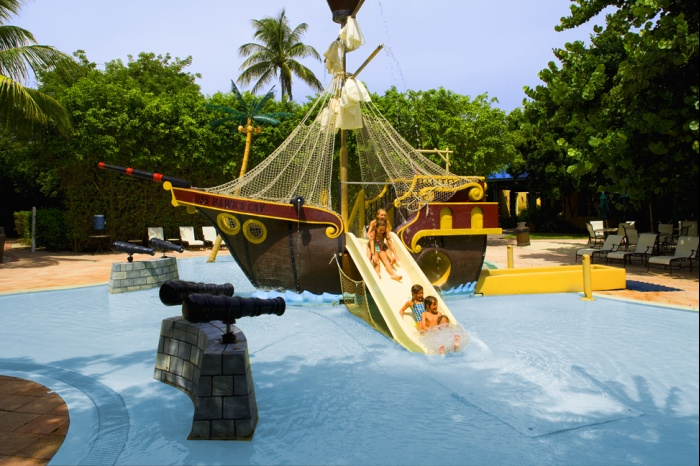
\includegraphics[width=0.75\linewidth]{images/pirateswimming} 

}

\caption{Despite what you might find at family friendly waterparks -- this is NOT how real pirate swimming lessons look.}\label{fig:unnamed-chunk-30}
\end{figure}

What's the first exercise on the first day of pirate swimming lessons?
While it would be cute if they all had little inflatable pirate ships to
swim around in -- unfortunately this is not the case. Instead, those
baby pirates take a walk off their baby planks so they can get a taste
of what they're in for. Turns out, learning R is the same way. Let's
jump in. In this chapter, you'll see how easy it is to calculate basic
statistics and create plots in R. Don't worry if the code you're running
doesn't make immediate sense -- just marvel at how easy it is to do this
in R!

In this section, we'll analyze a dataset called\ldots{}wait for
it\ldots{}pirates! The dataset contains data from a survey of 1,000
pirates. The data is contained in the \texttt{yarrr} package, so make
sure you've installed and loaded the package:

\begin{Shaded}
\begin{Highlighting}[]
\CommentTok{# Install the yarrr package}
\KeywordTok{install.packages}\NormalTok{(}\StringTok{'yarrr'}\NormalTok{)}

\CommentTok{# Load the package}
\KeywordTok{library}\NormalTok{(yarrr)}
\end{Highlighting}
\end{Shaded}

\section{Exploring data}\label{exploring-data}

Next, we'll look at the help menu for the pirates dataset using the
question mark \texttt{?pirates}. When you run this, you should see a
small help window open up in RStudio that gives you some information
about the dataset.

\begin{Shaded}
\begin{Highlighting}[]
\NormalTok{?pirates}
\end{Highlighting}
\end{Shaded}

First, let's take a look at the first few rows of the dataset using the
\texttt{head()} function. This will show you the first few rows of the
data.

\begin{Shaded}
\begin{Highlighting}[]
\CommentTok{# Look at the first few rows of the data}
\KeywordTok{head}\NormalTok{(pirates)}
\NormalTok{##      id  sex age height weight headband college tattoos tchests parrots}
\NormalTok{## 2     2 male  31    209    106      yes   JSSFP       9      11       0}
\NormalTok{## 793 793 male  25    209    104      yes    CCCC       8      27       9}
\NormalTok{## 430 430 male  26    201     99      yes    CCCC       4       7       1}
\NormalTok{## 292 292 male  29    201    102      yes    CCCC       9       2       3}
\NormalTok{## 895 895 male  27    201    103      yes    CCCC      12       1       1}
\NormalTok{## 409 409 male  28    201     97      yes    CCCC       7      10       0}
\NormalTok{##     favorite.pirate sword.type eyepatch sword.time beard.length}
\NormalTok{## 2      Jack Sparrow    cutlass        0        1.1           21}
\NormalTok{## 793        Anicetus    cutlass        1        1.1           16}
\NormalTok{## 430    Jack Sparrow    cutlass        1        0.9           14}
\NormalTok{## 292    Jack Sparrow      sabre        1        9.9           14}
\NormalTok{## 895            Hook    cutlass        1        2.3           25}
\NormalTok{## 409    Jack Sparrow    cutlass        1        1.2           15}
\NormalTok{##               fav.pixar grogg}
\NormalTok{## 2                WALL-E     9}
\NormalTok{## 793 Monsters University     8}
\NormalTok{## 430              WALL-E     9}
\NormalTok{## 292              WALL-E     6}
\NormalTok{## 895               Brave    14}
\NormalTok{## 409          Inside Out     7}
\end{Highlighting}
\end{Shaded}

You can look at the names of the columns in the dataset with the
\texttt{names()} function

\begin{Shaded}
\begin{Highlighting}[]
\CommentTok{# What are the names of the columns?}
\KeywordTok{names}\NormalTok{(pirates)}
\NormalTok{##  [1] "id"              "sex"             "age"            }
\NormalTok{##  [4] "height"          "weight"          "headband"       }
\NormalTok{##  [7] "college"         "tattoos"         "tchests"        }
\NormalTok{## [10] "parrots"         "favorite.pirate" "sword.type"     }
\NormalTok{## [13] "eyepatch"        "sword.time"      "beard.length"   }
\NormalTok{## [16] "fav.pixar"       "grogg"}
\end{Highlighting}
\end{Shaded}

Finally, you can also view the entire dataset in a separate window using
the \texttt{View()} function:

\begin{Shaded}
\begin{Highlighting}[]
\CommentTok{# View the entire dataset in a new window}
\KeywordTok{View}\NormalTok{(pirates)}
\end{Highlighting}
\end{Shaded}

\section{Descriptive statistics}\label{descriptive-statistics}

Now let's calculate some basic statistics on the entire dataset. We'll
calculate the mean age, maximum height, and number of pirates of each
sex:

\begin{Shaded}
\begin{Highlighting}[]
\CommentTok{# What is the mean age?}
\KeywordTok{mean}\NormalTok{(pirates}\OperatorTok{$}\NormalTok{age)}
\NormalTok{## [1] 27}

\CommentTok{# What was the tallest pirate?}
\KeywordTok{max}\NormalTok{(pirates}\OperatorTok{$}\NormalTok{height)}
\NormalTok{## [1] 209}

\CommentTok{# How many pirates are there of each sex?}
\KeywordTok{table}\NormalTok{(pirates}\OperatorTok{$}\NormalTok{sex)}
\NormalTok{## }
\NormalTok{## female   male  other }
\NormalTok{##    464    490     46}
\end{Highlighting}
\end{Shaded}

Now, let's calculate statistics for different groups of pirates. For
example, the following code will use the \texttt{aggregate()} function
to calculate the mean age of pirates, separately for each sex.

\begin{Shaded}
\begin{Highlighting}[]
\CommentTok{# Calculate the mean age, separately for each sex}
\KeywordTok{aggregate}\NormalTok{(}\DataTypeTok{formula =}\NormalTok{ age }\OperatorTok{~}\StringTok{ }\NormalTok{sex,}
          \DataTypeTok{data =}\NormalTok{ pirates,}
          \DataTypeTok{FUN =}\NormalTok{ mean)}
\NormalTok{##      sex age}
\NormalTok{## 1 female  30}
\NormalTok{## 2   male  25}
\NormalTok{## 3  other  27}
\end{Highlighting}
\end{Shaded}

\section{Plotting}\label{plotting}

Cool stuff, now let's make a plot! We'll plot the relationship between
pirate's height and weight using the \texttt{plot()} function

\begin{Shaded}
\begin{Highlighting}[]
\CommentTok{# Create scatterplot}
\KeywordTok{plot}\NormalTok{(}\DataTypeTok{x =}\NormalTok{ pirates}\OperatorTok{$}\NormalTok{height,        }\CommentTok{# X coordinates}
     \DataTypeTok{y =}\NormalTok{ pirates}\OperatorTok{$}\NormalTok{weight)        }\CommentTok{# y-coordinates}
\end{Highlighting}
\end{Shaded}

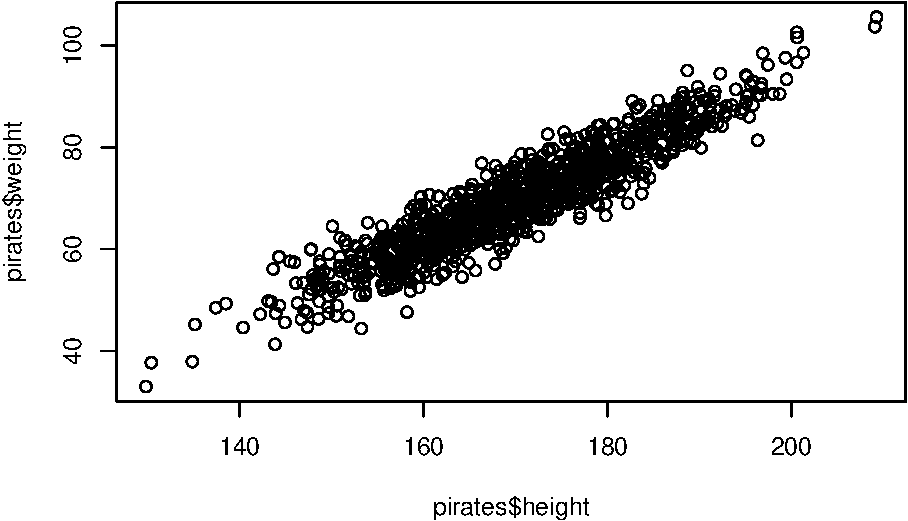
\includegraphics{YaRrr_files/figure-latex/unnamed-chunk-38-1.pdf}

Now let's make a fancier version of the same plot by adding some
customization

\begin{Shaded}
\begin{Highlighting}[]
\CommentTok{# Create scatterplot}
\KeywordTok{plot}\NormalTok{(}\DataTypeTok{x =}\NormalTok{ pirates}\OperatorTok{$}\NormalTok{height,        }\CommentTok{# X coordinates}
     \DataTypeTok{y =}\NormalTok{ pirates}\OperatorTok{$}\NormalTok{weight,        }\CommentTok{# y-coordinates}
     \DataTypeTok{main =} \StringTok{'My first scatterplot of pirate data!'}\NormalTok{,}
     \DataTypeTok{xlab =} \StringTok{'Height (in cm)'}\NormalTok{,   }\CommentTok{# x-axis label}
     \DataTypeTok{ylab =} \StringTok{'Weight (in kg)'}\NormalTok{,   }\CommentTok{# y-axis label}
     \DataTypeTok{pch =} \DecValTok{16}\NormalTok{,                  }\CommentTok{# Filled circles}
     \DataTypeTok{col =} \KeywordTok{gray}\NormalTok{(.}\DecValTok{0}\NormalTok{, .}\DecValTok{1}\NormalTok{))        }\CommentTok{# Transparent gray}
\end{Highlighting}
\end{Shaded}

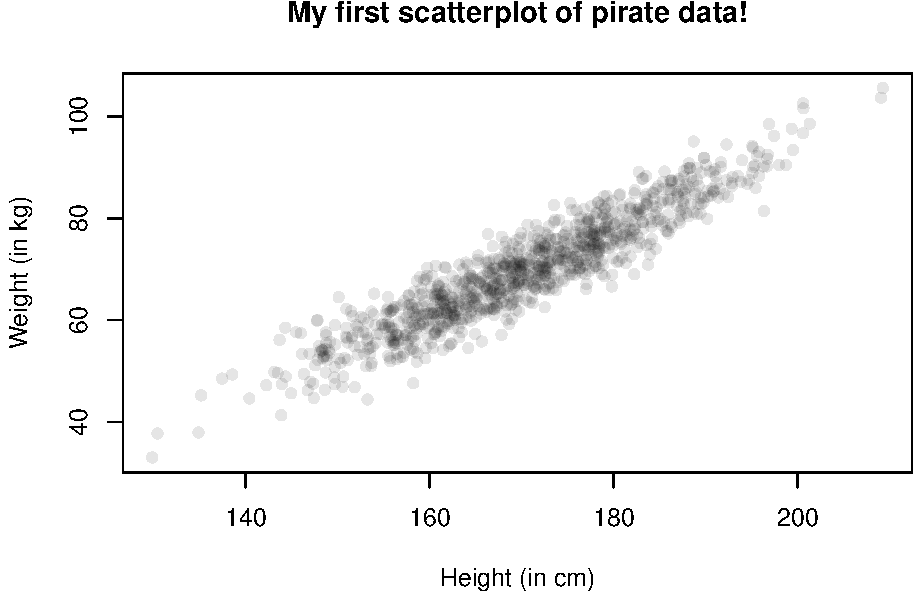
\includegraphics{YaRrr_files/figure-latex/unnamed-chunk-39-1.pdf}

Now let's make it even better by adding gridlines and a blue regression
line to measure the strength of the relationship.

\begin{Shaded}
\begin{Highlighting}[]
\CommentTok{# Create scatterplot}
\KeywordTok{plot}\NormalTok{(}\DataTypeTok{x =}\NormalTok{ pirates}\OperatorTok{$}\NormalTok{height,        }\CommentTok{# X coordinates}
     \DataTypeTok{y =}\NormalTok{ pirates}\OperatorTok{$}\NormalTok{weight,        }\CommentTok{# y-coordinates}
     \DataTypeTok{main =} \StringTok{'My first scatterplot of pirate data!'}\NormalTok{,}
     \DataTypeTok{xlab =} \StringTok{'Height (in cm)'}\NormalTok{,   }\CommentTok{# x-axis label}
     \DataTypeTok{ylab =} \StringTok{'Weight (in kg)'}\NormalTok{,   }\CommentTok{# y-axis label}
     \DataTypeTok{pch =} \DecValTok{16}\NormalTok{,                  }\CommentTok{# Filled circles}
     \DataTypeTok{col =} \KeywordTok{gray}\NormalTok{(.}\DecValTok{0}\NormalTok{, .}\DecValTok{1}\NormalTok{))        }\CommentTok{# Transparent gray}

\KeywordTok{grid}\NormalTok{()        }\CommentTok{# Add gridlines}

\CommentTok{# Create a linear regression model}
\NormalTok{model <-}\StringTok{ }\KeywordTok{lm}\NormalTok{(}\DataTypeTok{formula =}\NormalTok{ weight }\OperatorTok{~}\StringTok{ }\NormalTok{height, }
            \DataTypeTok{data =}\NormalTok{ pirates)}

\KeywordTok{abline}\NormalTok{(model, }\DataTypeTok{col =} \StringTok{'blue'}\NormalTok{)      }\CommentTok{# Add regression to plot}
\end{Highlighting}
\end{Shaded}

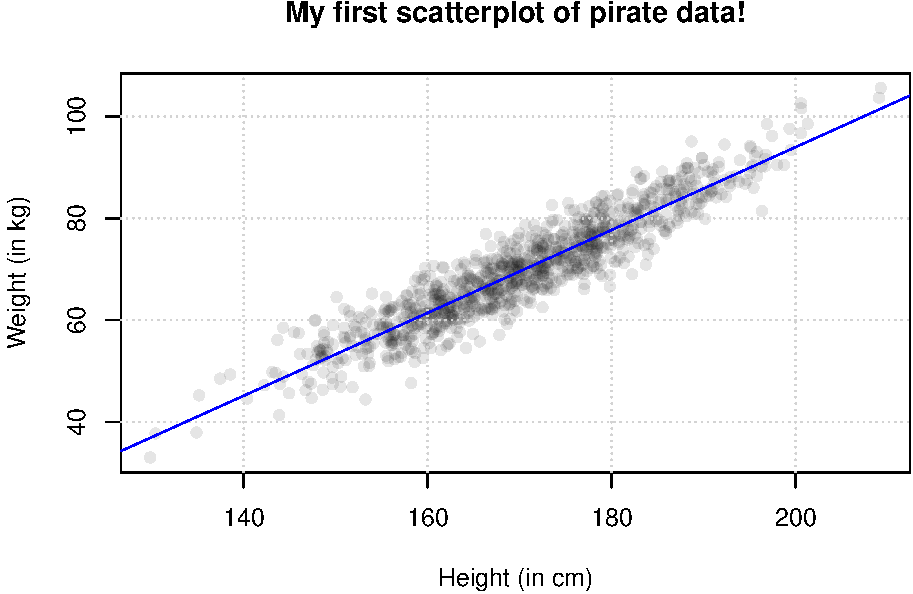
\includegraphics{YaRrr_files/figure-latex/unnamed-chunk-40-1.pdf}

Scatterplots are great for showing the relationship between two
continuous variables, but what if your independent variable is not
continuous? In this case, pirateplots are a good option. Let's create a
pirateplot using the \texttt{pirateplot()} function to show the
distribution of pirate's age based on their favorite sword:

\begin{Shaded}
\begin{Highlighting}[]
\KeywordTok{pirateplot}\NormalTok{(}\DataTypeTok{formula =}\NormalTok{ age }\OperatorTok{~}\StringTok{ }\NormalTok{sword.type, }
           \DataTypeTok{data =}\NormalTok{ pirates,}
           \DataTypeTok{main =} \StringTok{"Pirateplot of ages by favorite sword"}\NormalTok{)}
\end{Highlighting}
\end{Shaded}

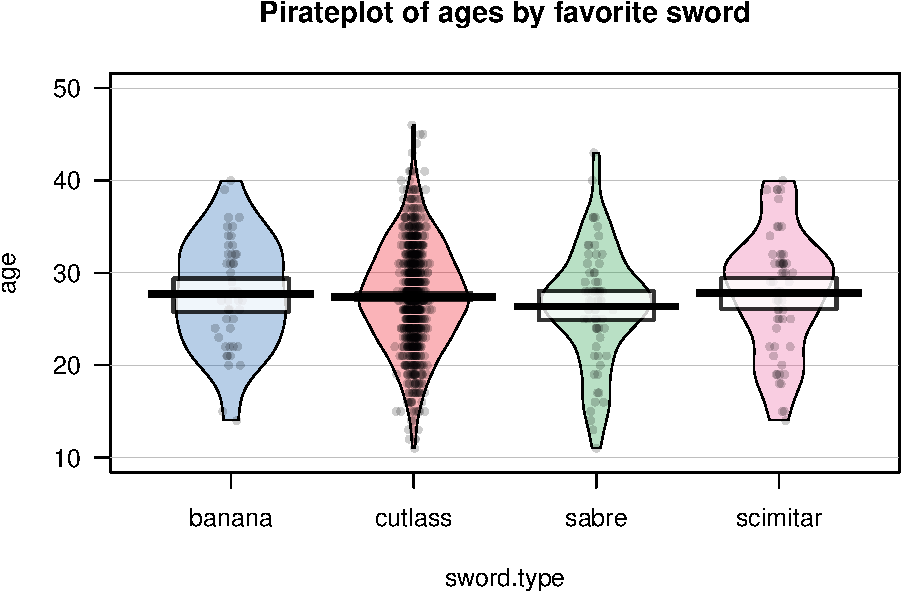
\includegraphics{YaRrr_files/figure-latex/unnamed-chunk-41-1.pdf}

Now let's make another pirateplot showing the relationship between sex
and height using a different plotting theme and the \texttt{"pony"}
color palette:

\begin{Shaded}
\begin{Highlighting}[]
\KeywordTok{pirateplot}\NormalTok{(}\DataTypeTok{formula =}\NormalTok{ height }\OperatorTok{~}\StringTok{ }\NormalTok{sex,               }\CommentTok{# Plot weight as a function of sex}
           \DataTypeTok{data =}\NormalTok{ pirates,                       }
           \DataTypeTok{main =} \StringTok{"Pirateplot of height by sex"}\NormalTok{,}
           \DataTypeTok{pal =} \StringTok{"pony"}\NormalTok{,                         }\CommentTok{# Use the info color palette}
           \DataTypeTok{theme =} \DecValTok{3}\NormalTok{)                            }\CommentTok{# Use theme 3}
\end{Highlighting}
\end{Shaded}

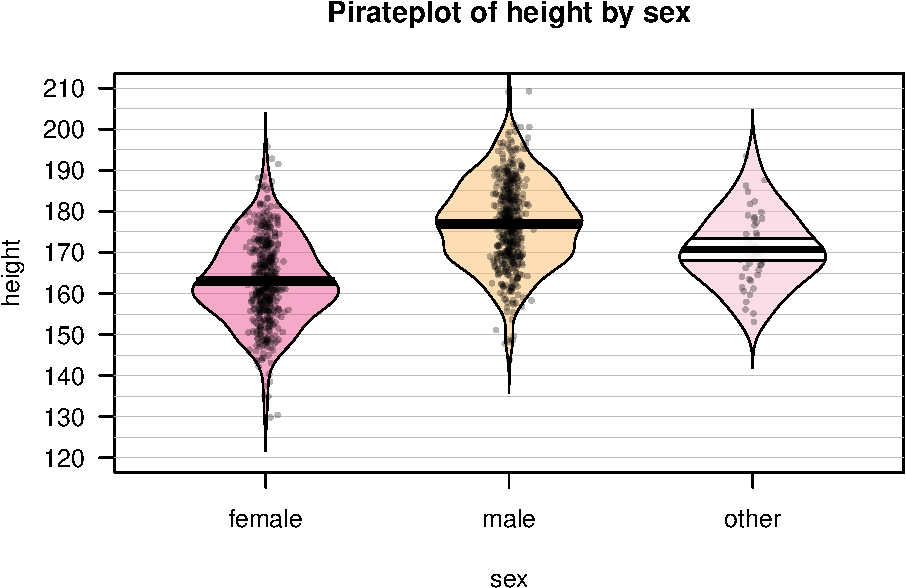
\includegraphics{YaRrr_files/figure-latex/unnamed-chunk-42-1.pdf}

The \texttt{"pony"} palette is contained in the \texttt{piratepal()}
function. Let's see where the \texttt{"pony"} palette comes from\ldots{}

\begin{Shaded}
\begin{Highlighting}[]
\CommentTok{# Show me the pony palette!}
\KeywordTok{piratepal}\NormalTok{(}\DataTypeTok{palette =} \StringTok{"pony"}\NormalTok{,}
          \DataTypeTok{plot.result =} \OtherTok{TRUE}\NormalTok{,   }\CommentTok{# Plot the result}
          \DataTypeTok{trans =}\NormalTok{ .}\DecValTok{1}\NormalTok{)           }\CommentTok{# Slightly transparent}
\end{Highlighting}
\end{Shaded}

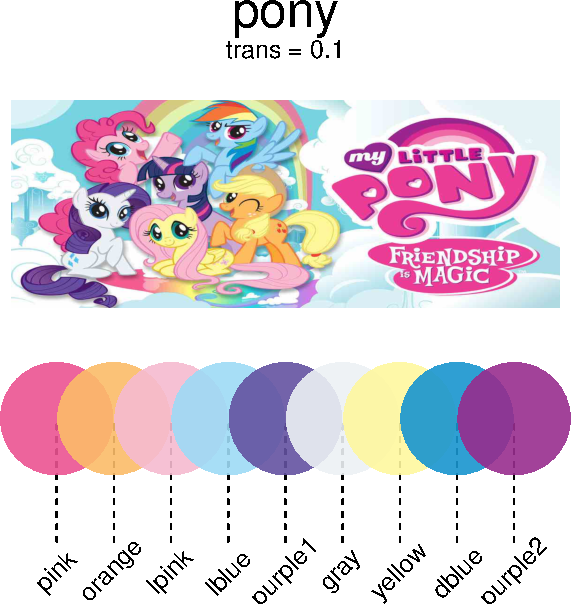
\includegraphics{YaRrr_files/figure-latex/unnamed-chunk-43-1.pdf}

\section{Hypothesis tests}\label{hypothesis-tests}

Now, let's do some basic hypothesis tests. First, let's conduct a
two-sample t-test to see if there is a significant difference between
the ages of pirates who do wear a headband, and those who do not:

\begin{Shaded}
\begin{Highlighting}[]
\CommentTok{# Age by headband t-test}
\KeywordTok{t.test}\NormalTok{(}\DataTypeTok{formula =}\NormalTok{ age }\OperatorTok{~}\StringTok{ }\NormalTok{headband,}
       \DataTypeTok{data =}\NormalTok{ pirates,}
       \DataTypeTok{alternative =} \StringTok{'two.sided'}\NormalTok{)}
\NormalTok{## }
\NormalTok{##  Welch Two Sample t-test}
\NormalTok{## }
\NormalTok{## data:  age by headband}
\NormalTok{## t = 0.4, df = 100, p-value = 0.7}
\NormalTok{## alternative hypothesis: true difference in means is not equal to 0}
\NormalTok{## 95 percent confidence interval:}
\NormalTok{##  -1.0  1.5}
\NormalTok{## sample estimates:}
\NormalTok{##  mean in group no mean in group yes }
\NormalTok{##                28                27}
\end{Highlighting}
\end{Shaded}

With a p-value of 0.7259, we don't have sufficient evidence say there is
a difference in the men age of pirates who wear headbands and those that
do not.

Next, let's test if there a significant correlation between a pirate's
height and weight using the \texttt{cor.test()} function:

\begin{Shaded}
\begin{Highlighting}[]
\KeywordTok{cor.test}\NormalTok{(}\DataTypeTok{formula =} \OperatorTok{~}\StringTok{ }\NormalTok{height }\OperatorTok{+}\StringTok{ }\NormalTok{weight,}
         \DataTypeTok{data =}\NormalTok{ pirates)}
\NormalTok{## }
\NormalTok{##  Pearson's product-moment correlation}
\NormalTok{## }
\NormalTok{## data:  height and weight}
\NormalTok{## t = 80, df = 1000, p-value <2e-16}
\NormalTok{## alternative hypothesis: true correlation is not equal to 0}
\NormalTok{## 95 percent confidence interval:}
\NormalTok{##  0.92 0.94}
\NormalTok{## sample estimates:}
\NormalTok{##  cor }
\NormalTok{## 0.93}
\end{Highlighting}
\end{Shaded}

We got a p-value of \texttt{p\ \textless{}\ 2.2e-16}, that's scientific
notation for \texttt{p\ \textless{}\ .00000000000000016} -- which is
pretty much 0. Thus, we'd conclude that there is a significant
(positive) relationship between a pirate's height and weight.

Now, let's do an ANOVA testing if there is a difference between the
number of tattoos pirates have based on their favorite sword

\begin{Shaded}
\begin{Highlighting}[]
\CommentTok{# Create tattoos model}
\NormalTok{tat.sword.lm <-}\StringTok{ }\KeywordTok{lm}\NormalTok{(}\DataTypeTok{formula =}\NormalTok{ tattoos }\OperatorTok{~}\StringTok{ }\NormalTok{sword.type,}
                   \DataTypeTok{data =}\NormalTok{ pirates)}

\CommentTok{# Get ANOVA table}
\KeywordTok{anova}\NormalTok{(tat.sword.lm)}
\NormalTok{## Analysis of Variance Table}
\NormalTok{## }
\NormalTok{## Response: tattoos}
\NormalTok{##             Df Sum Sq Mean Sq F value Pr(>F)    }
\NormalTok{## sword.type   3   1588     529    54.1 <2e-16 ***}
\NormalTok{## Residuals  996   9743      10                   }
\NormalTok{## ---}
\NormalTok{## Signif. codes:  0 '***' 0.001 '**' 0.01 '*' 0.05 '.' 0.1 ' ' 1}
\end{Highlighting}
\end{Shaded}

Sure enough, we see another very small p-value of
\texttt{p\ \textless{}\ 2.2e-16}, suggesting that the number of tattoos
pirate's have are different based on their favorite sword.

\section{Regression analysis}\label{regression-analysis}

Finally, let's run a regression analysis to see if a pirate's age,
weight, and number of tattoos (s)he has predicts how many treasure
chests he/she's found:

\begin{Shaded}
\begin{Highlighting}[]
\CommentTok{# Create a linear regression model: DV = tchests, IV = age, weight, tattoos}
\NormalTok{tchests.model <-}\StringTok{ }\KeywordTok{lm}\NormalTok{(}\DataTypeTok{formula =}\NormalTok{ tchests }\OperatorTok{~}\StringTok{ }\NormalTok{age }\OperatorTok{+}\StringTok{ }\NormalTok{weight }\OperatorTok{+}\StringTok{ }\NormalTok{tattoos,}
                    \DataTypeTok{data =}\NormalTok{ pirates)}

\CommentTok{# Show summary statistics}
\KeywordTok{summary}\NormalTok{(tchests.model)}
\NormalTok{## }
\NormalTok{## Call:}
\NormalTok{## lm(formula = tchests ~ age + weight + tattoos, data = pirates)}
\NormalTok{## }
\NormalTok{## Residuals:}
\NormalTok{##    Min     1Q Median     3Q    Max }
\NormalTok{## -33.30 -15.83  -6.86   8.41 119.97 }
\NormalTok{## }
\NormalTok{## Coefficients:}
\NormalTok{##             Estimate Std. Error t value Pr(>|t|)    }
\NormalTok{## (Intercept)   5.1908     7.1844    0.72     0.47    }
\NormalTok{## age           0.7818     0.1344    5.82    8e-09 ***}
\NormalTok{## weight       -0.0901     0.0718   -1.25     0.21    }
\NormalTok{## tattoos       0.2540     0.2255    1.13     0.26    }
\NormalTok{## ---}
\NormalTok{## Signif. codes:  0 '***' 0.001 '**' 0.01 '*' 0.05 '.' 0.1 ' ' 1}
\NormalTok{## }
\NormalTok{## Residual standard error: 24 on 996 degrees of freedom}
\NormalTok{## Multiple R-squared:  0.0406, Adjusted R-squared:  0.0377 }
\NormalTok{## F-statistic:   14 on 3 and 996 DF,  p-value: 5.75e-09}
\end{Highlighting}
\end{Shaded}

It looks like the only significant predictor of the number of treasure
chests that a pirate has found is his/her age. There does not seem to be
significant effect of weight or tattoos.

\section{Bayesian Statistics}\label{bayesian-statistics}

Now, let's repeat some of our previous analyses with Bayesian versions.
First we'll install and load the \texttt{BayesFactor} package which
contains the Bayesian statistics functions we'll use:

\begin{Shaded}
\begin{Highlighting}[]
\CommentTok{# Install and load the BayesFactor package}
\KeywordTok{install.packages}\NormalTok{(}\StringTok{'BayesFactor'}\NormalTok{)}
\KeywordTok{library}\NormalTok{(BayesFactor)}
\end{Highlighting}
\end{Shaded}

Now that the packages is installed and loaded, we're good to go! Let's
do a Bayesian version of our earlier t-test asking if pirates who wear a
headband are older or younger than those who do not.

\begin{Shaded}
\begin{Highlighting}[]
\CommentTok{# Bayesian t-test comparing the age of pirates with and without headbands}
\KeywordTok{ttestBF}\NormalTok{(}\DataTypeTok{formula =}\NormalTok{ age }\OperatorTok{~}\StringTok{ }\NormalTok{headband,}
        \DataTypeTok{data =}\NormalTok{ pirates)}
\NormalTok{## Bayes factor analysis}
\NormalTok{## --------------}
\NormalTok{## [1] Alt., r=0.707 : 0.12 ±0%}
\NormalTok{## }
\NormalTok{## Against denominator:}
\NormalTok{##   Null, mu1-mu2 = 0 }
\NormalTok{## ---}
\NormalTok{## Bayes factor type: BFindepSample, JZS}
\end{Highlighting}
\end{Shaded}

It looks like we got a Bayes factor of 0.12 which is strong evidence
\emph{for} the null hypothesis (that the mean age does not differ
between pirates with and without headbands)

\section{Wasn't that easy?!}\label{wasnt-that-easy}

Wait\ldots{}wait\ldots{}WAIT! Did you seriously just calculate
descriptive statistics, a t-test, an ANOVA, and a regression, create a
scatterplot and a pirateplot, AND do both a Bayesian t-test and
regression analysis. Yup. Imagine how long it would have taken to
explain how to do all that in SPSS. And while you haven't really learned
how R works yet, I'd bet my beard that you could easily alter the
previous code to do lots of other analyses. Of course, don't worry if
some or all of the previous code didn't make sense. Soon\ldots{}it will
all be clear.

Now that you've jumped in, let's learn how to swim.

\chapter{The Basics}\label{basics}

If you're like most people, you think of R as a statistics program.
However, while R is definitely the coolest, most badass, pirate-y way to
conduct statistics -- it's not really a program. Rather, it's a
programming \emph{language} that was written by and for statisticians.
To learn more about the history of R\ldots{}just\ldots{}you
know\ldots{}Google it.

\begin{figure}

{\centering 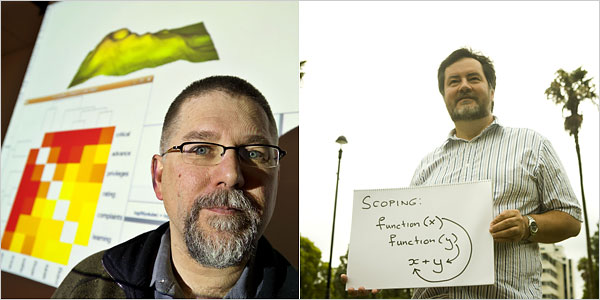
\includegraphics[width=0.5\linewidth]{images/rauthors} 

}

\caption{Ross Ihaka and Robert Gentlemen. You have these two pirates to thank for creating R! You might not think much of them now, but by the end of this book there's a good chance you'll be dressing up as one of them on Halloween.}\label{fig:unnamed-chunk-51}
\end{figure}

In this chapter, we'll go over the basics of the R language and the
RStudio programming environment.

\section{The command-line (Console)}\label{the-command-line-console}

\begin{figure}

{\centering 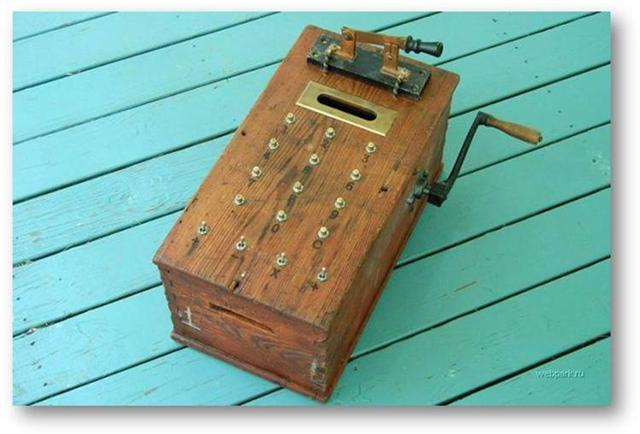
\includegraphics[width=0.5\linewidth]{images/woodcalc} 

}

\caption{Yep. R is really just a fancy calculator. This R programming device was found on a shipwreck on the Bodensee in Germany. I stole it from a museum and made a pretty sweet plot with it. But I don't want to show it to you.}\label{fig:unnamed-chunk-52}
\end{figure}

R code, on its own, is just text. You can write R code in a new script
within R or RStudio, or in any text editor. Hell, you can write R code
on Twitter if you want. However, just writing the code won't do the
whole job -- in order for your code to be executed (aka, interpreted)
you need to send it to R's \emph{command-line interpreter}. In RStudio,
the command-line interpreter is called the Console.

\begin{figure}

{\centering 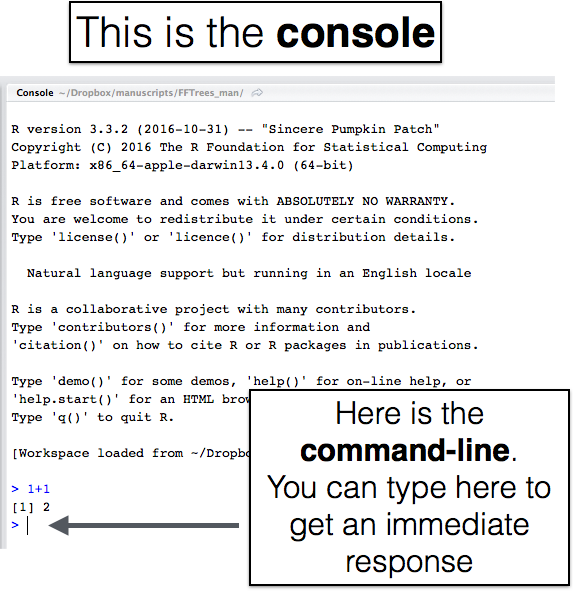
\includegraphics[width=0.75\linewidth]{images/commandline} 

}

\caption{You can always type code directly into the command line to get an immediate response.}\label{fig:unnamed-chunk-53}
\end{figure}

In R, the command-line interpreter starts with the
\texttt{\textgreater{}} symbol. This is called the \textbf{prompt}. Why
is it called the prompt? Well, it's ``prompting'' you to feed it with
some R code. The fastest way to have R evaluate code is to type your R
code directly into the command-line interpreter. For example, if you
type \texttt{1+1} into the interpreter and hit enter you'll see the
following

\begin{Shaded}
\begin{Highlighting}[]
\DecValTok{1}\OperatorTok{+}\DecValTok{1}
\NormalTok{## [1] 2}
\end{Highlighting}
\end{Shaded}

As you can see, R returned the (thankfully correct) value of 2. You'll
notice that the console also returns the text {[}1{]}. This is just
telling you you the index of the value next to it. Don't worry about
this for now, it will make more sense later. As you can see, R can,
thankfully, do basic calculations. In fact, at its heart, R is
technically just a fancy calculator. But that's like saying Michael
Jordan is \emph{just} a fancy ball bouncer or Donald Trump is
\emph{just} an orange with a dead fox on his head. It (and they), are
much more than that.

\section{Writing R scripts in an
editor}\label{writing-r-scripts-in-an-editor}

There are certainly many cases where it makes sense to type code
directly into the console. For example, to open a help menu for a new
function with the ? command, to take a quick look at a dataset with the
\texttt{head()} function, or to do simple calculations like
\texttt{1+1}, you should type directly into the console. However, the
problem with writing all your code in the console is that nothing that
you write will be saved. So if you make an error, or want to make a
change to some earlier code, you have to type it all over again. Not
very efficient. For this (and many more reasons), you'll should write
any important code that you want to save as an R script. An R script is
just a bunch of R code in a single file. You can write an R script in
any text editor, but you should save it with the \texttt{.R} suffix to
make it clear that it contains R code.\} in an editor.

In RStudio, you'll write your R code in the\ldots{}wait for
it\ldots{}\emph{Source} window. To start writing a new R script in
RStudio, click File -- New File -- R Script.

\textbf{Shortcut!} To create a new script in R, you can also use the
command--shift--N shortcut on Mac. I don't know what it is on
PC\ldots{}and I don't want to know.

When you open a new script, you'll see a blank page waiting for you to
write as much R code as you'd like. In Figure \ref{fig:editor}, I have a
new script called \texttt{examplescript} with a few random calculations.

\begin{figure}

{\centering 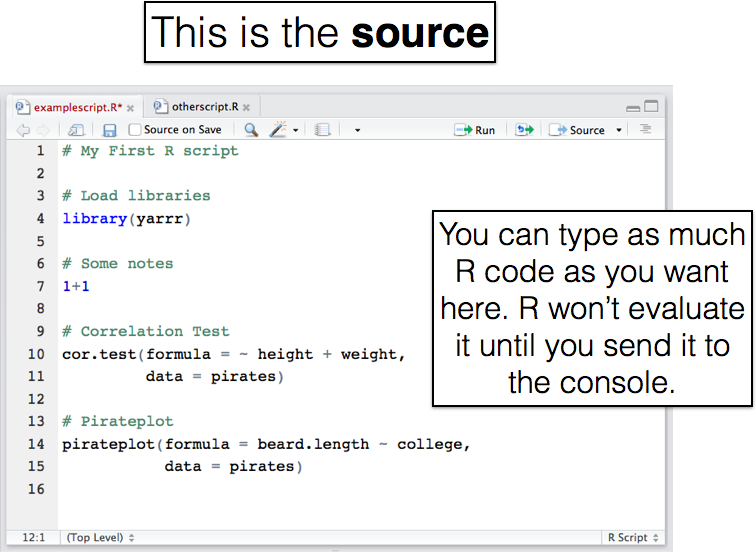
\includegraphics[width=0.75\linewidth]{images/sourcess} 

}

\caption{Here's how a new script looks in the editor window on RStudio. The code you type won't be executed until you send it to the console.}\label{fig:editor}
\end{figure}

You can have several R scripts open in the source window in separate
tabs (like I have above).

\subsection{Send code from an source to the
console}\label{send-code-from-an-source-to-the-console}

\begin{figure}

{\centering 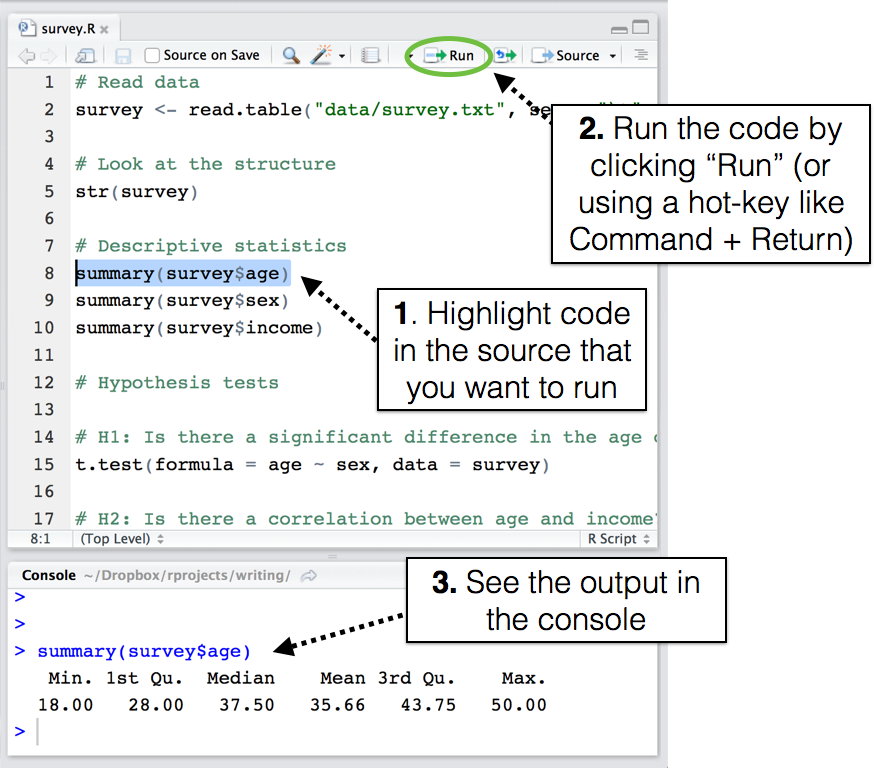
\includegraphics[width=0.75\linewidth]{images/runningcode} 

}

\caption{To evaluate code from the source, highlight it and run it.}\label{fig:runcode}
\end{figure}

When you type code into an R script, you'll notice that, unlike typing
code into the Console, nothing happens. In order for R to interpret the
code, you need to send it from the Editor to the Console. There are a
few ways to do this, here are the three most common ways:

\begin{enumerate}
\def\labelenumi{\arabic{enumi}.}
\item
  Copy the code from the Editor (or anywhere that has valid R code), and
  paste it into the Console (using Command--V).
\item
  Highlight the code you want to run (with your mouse or by holding
  Shift), then use the Command--Return shortcut (see Figure
  \ref{fig:commandreturn}).
\item
  Place the cursor on a single line you want to run, then use the
  Command--Return shortcut to run just that line.
\end{enumerate}

\begin{figure}

{\centering 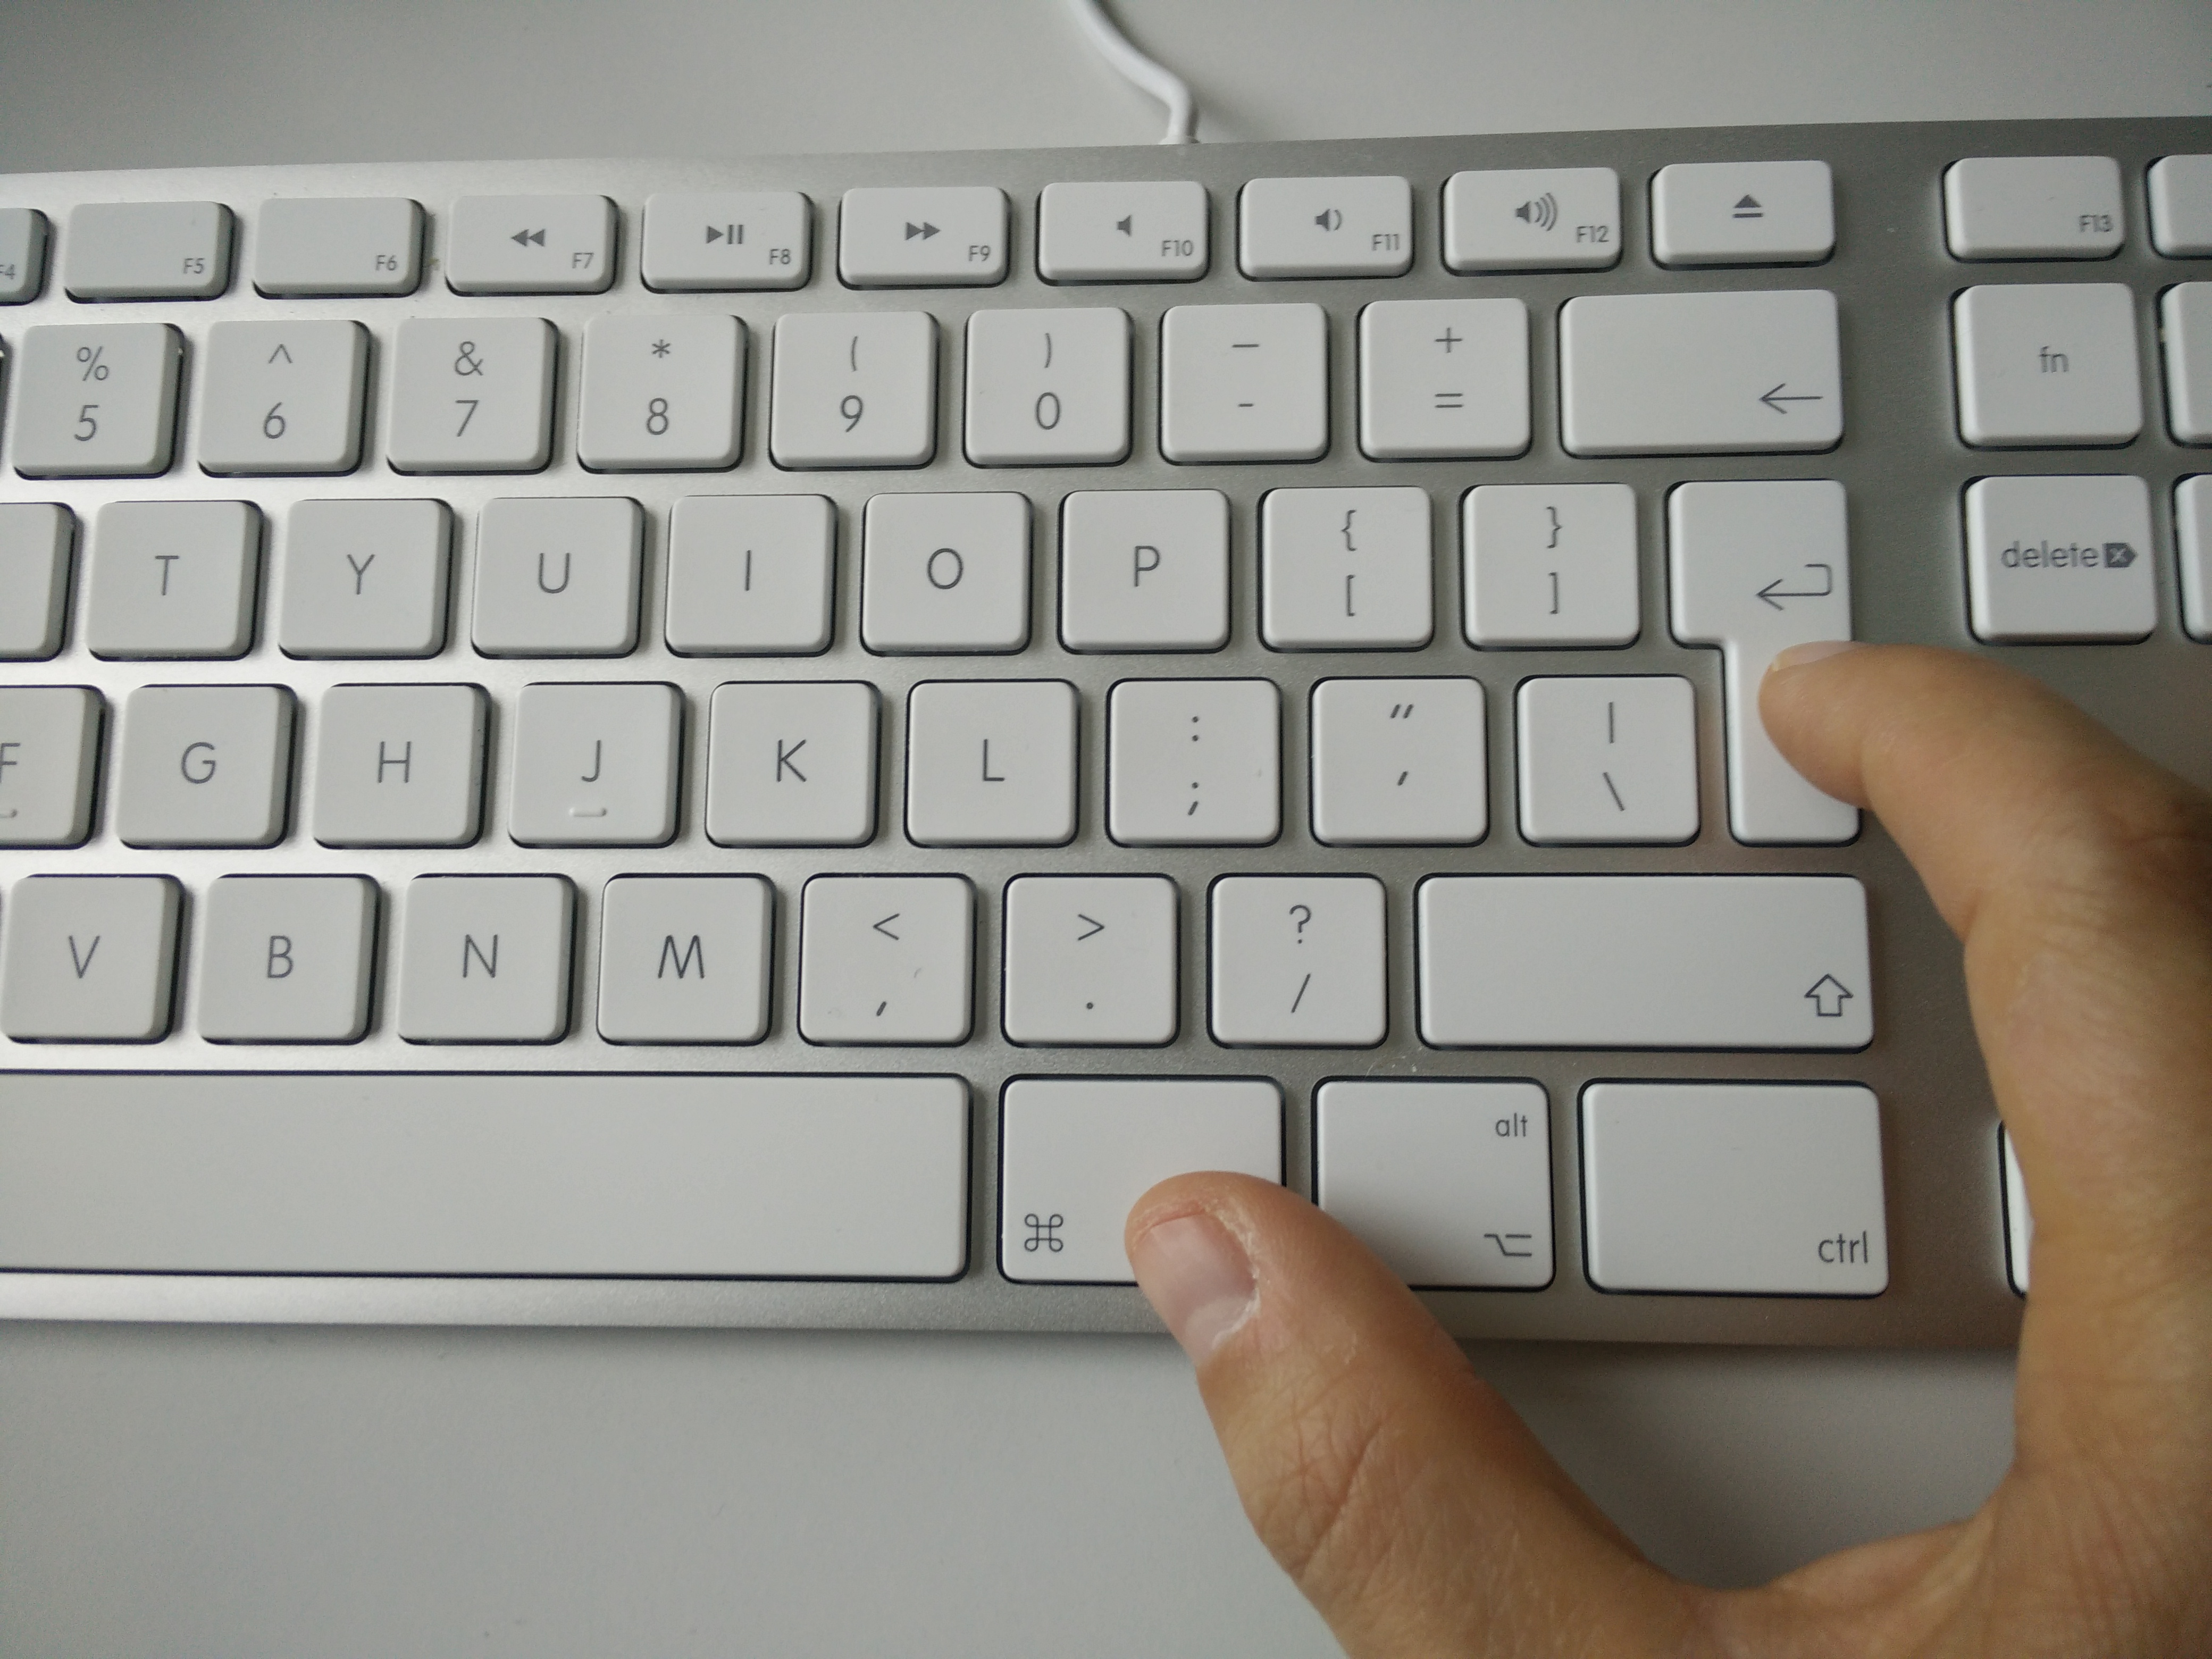
\includegraphics[width=0.5\linewidth]{images/commandreturn} 

}

\caption{Ah...the Command--Return shortcut (Control--Enter on PC) to send highlighted code from the Editor to the Console. Get used to this shortcut people. You're going to be using this a lot}\label{fig:commandreturn}
\end{figure}

99\% of the time, I use method 2, where I highlight the code I want,
then use the Command--Return shortcut . However, method 3 is great for
trouble-shooting code line-by-line.

\section{A brief style guide: Commenting and
spacing}\label{a-brief-style-guide-commenting-and-spacing}

Like all programming languages, R isn't just meant to be read by a
computer, it's also meant to be read by other humans -- or very
well-trained dolphins. For this reason, it's important that your code
looks nice and is understandable to other people and your future self.
To keep things brief, I won't provide a complete style guide -- instead
I'll focus on the two most critical aspects of good style: commenting
and spacing.

\begin{figure}

{\centering 
\includegraphics[width=0.5\linewidth]{images/futureself} 

}

\caption{As Stan discovered in season six of South Park, your future self is a lazy, possibly intoxicated moron. So do your future self a favor and make your code look nice. Also maybe go for a run once in a while.}\label{fig:futureself}
\end{figure}

\subsection{Commenting code with the \# (pound)
sign}\label{commenting-code-with-the-pound-sign}

Comments are completely ignored by R and are just there for whomever is
reading the code. You can use comments to explain what a certain line of
code is doing, or just to visually separate meaningful chunks of code
from each other. Comments in R are designated by a \# (pound) sign.
Whenever R encounters a \# sign, it will ignore \textbf{all} the code
after the \# sign on that line. Additionally, in most coding editors
(like RStudio) the editor will display comments in a separate color than
standard R code to remind you that it's a comment:

Here is an example of a short script that is nicely commented. Try to
make your scripts look like this!

\begin{Shaded}
\begin{Highlighting}[]
\CommentTok{# Author: Pirate Jack}
\CommentTok{# Title: My nicely commented R Script}
\CommentTok{# Date: None today :(}

\CommentTok{# Step 1: Load the yarrr package}
\KeywordTok{library}\NormalTok{(yarrr)}

\CommentTok{# Step 2: See the column names in the movies dataset}
\KeywordTok{names}\NormalTok{(movies)}

\CommentTok{# Step 3: Calculations}

\CommentTok{# What percent of movies are sequels?}
\KeywordTok{mean}\NormalTok{(movies}\OperatorTok{$}\NormalTok{sequel, }\DataTypeTok{na.rm =}\NormalTok{ T)}

\CommentTok{# How much did Pirate's of the Caribbean: On Stranger Tides make?}
\NormalTok{movies}\OperatorTok{$}\NormalTok{revenue.all[movies}\OperatorTok{$}\NormalTok{name }\OperatorTok{==}\StringTok{ 'Pirates of the Caribbean: On Stranger Tides'}\NormalTok{]}
\end{Highlighting}
\end{Shaded}

I cannot stress enough how important it is to comment your code! Trust
me, even if you don't plan on sharing your code with anyone else, keep
in mind that your future self will be reading it in the future.

\subsection{Spacing}\label{spacing}

Howwouldyouliketoreadabookiftherewerenospacesbetweenwords?
I'mguessingyouwouldn't.
Soeverytimeyouwritecodewithoutproperspacing,rememberthissentence.

Commenting isn't the only way to make your code legible. It's important
to make appropriate use of spaces and line breaks. For example, I
include spaces between arithmetic operators (like =, + and -) and after
commas (which we'll get to later). For example, look at the following
code:

\begin{figure}

{\centering 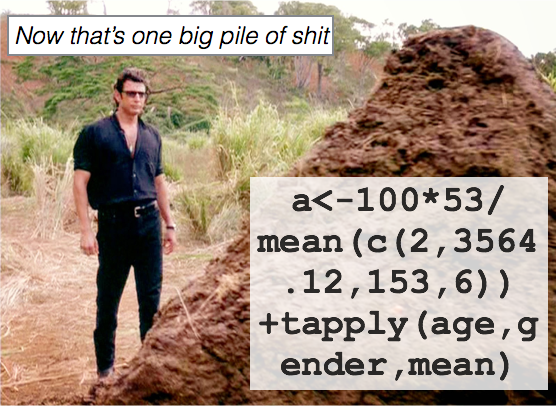
\includegraphics[width=0.5\linewidth]{images/pileofshit} 

}

\caption{Don't make your code look like what a sick Triceratops with diarrhea left behind for Jeff Goldblum.}\label{fig:pileofshit}
\end{figure}

\begin{Shaded}
\begin{Highlighting}[]
\CommentTok{# Shitty looking code}
\NormalTok{a<-(}\DecValTok{100}\OperatorTok{+}\DecValTok{3}\NormalTok{)}\OperatorTok{-}\DecValTok{2}
\KeywordTok{mean}\NormalTok{(}\KeywordTok{c}\NormalTok{(a}\OperatorTok{/}\DecValTok{100}\NormalTok{,}\FloatTok{642564624.34}\NormalTok{))}
\KeywordTok{t.test}\NormalTok{(}\DataTypeTok{formula=}\NormalTok{revenue.all}\OperatorTok{~}\NormalTok{sequel,}\DataTypeTok{data=}\NormalTok{movies)}
\KeywordTok{plot}\NormalTok{(}\DataTypeTok{x=}\NormalTok{movies}\OperatorTok{$}\NormalTok{budget,}\DataTypeTok{y=}\NormalTok{movies}\OperatorTok{$}\NormalTok{dvd.usa,}\DataTypeTok{main=}\StringTok{"myplot"}\NormalTok{)}
\end{Highlighting}
\end{Shaded}

That code looks like shit. Don't write code like that. It makes my eyes
hurt. Now, let's use some liberal amounts of commenting and spacing to
make it look less shitty.

\begin{Shaded}
\begin{Highlighting}[]
\CommentTok{# Some meaningless calculations. Not important}

\NormalTok{a <-}\StringTok{ }\NormalTok{(}\DecValTok{100} \OperatorTok{+}\StringTok{ }\DecValTok{3}\NormalTok{) }\OperatorTok{-}\StringTok{ }\DecValTok{2}
\KeywordTok{mean}\NormalTok{(}\KeywordTok{c}\NormalTok{(a }\OperatorTok{/}\StringTok{ }\DecValTok{100}\NormalTok{, }\FloatTok{642564624.34}\NormalTok{))}

\CommentTok{# t.test comparing revenue of sequels v non-sequels}

\KeywordTok{t.test}\NormalTok{(}\DataTypeTok{formula =}\NormalTok{ revenue.all }\OperatorTok{~}\StringTok{ }\NormalTok{sequel,}
       \DataTypeTok{data =}\NormalTok{ movies)}

\CommentTok{# A scatterplot of budget and dvd revenue. }
\CommentTok{#  Hard to see a relationship}

\KeywordTok{plot}\NormalTok{(}\DataTypeTok{x =}\NormalTok{ movies}\OperatorTok{$}\NormalTok{budget,}
     \DataTypeTok{y =}\NormalTok{ movies}\OperatorTok{$}\NormalTok{dvd.usa,}
     \DataTypeTok{main =} \StringTok{"myplot"}\NormalTok{)}
\end{Highlighting}
\end{Shaded}

See how much better that second chunk of code looks? Not only do the
comments tell us the purpose behind the code, but there are spaces and
line-breaks separating distinct elements.

There are a lot more aspects of good code formatting. For a list of
recommendations on how to make your code easier to follow, check out
Google's own company R Style guide at
\url{https://google-styleguide.googlecode.com/svn/trunk/Rguide.xml}

\section{Objects and functions}\label{objects-and-functions}

To understand how R works, you need to know that R revolves around two
things: objects and functions. Almost everything in R is either an
object or a function. In the following code chunk, I'll define a simple
object called \texttt{tattoos} using a function \texttt{c()}:

\begin{Shaded}
\begin{Highlighting}[]
\CommentTok{# 1: Create a vector object called tattoos}
\NormalTok{tattoos <-}\StringTok{ }\KeywordTok{c}\NormalTok{(}\DecValTok{4}\NormalTok{, }\DecValTok{67}\NormalTok{, }\DecValTok{23}\NormalTok{, }\DecValTok{4}\NormalTok{, }\DecValTok{10}\NormalTok{, }\DecValTok{35}\NormalTok{)}

\CommentTok{# 2: Apply the mean() function to the tattoos object}
\KeywordTok{mean}\NormalTok{(tattoos)}
\NormalTok{## [1] 24}
\end{Highlighting}
\end{Shaded}

What is an object? An object is a thing -- like a number, a dataset, a
summary statistic like a mean or standard deviation, or a statistical
test. Objects come in many different shapes and sizes in R. There are
simple objects like \textit{scalars} which represent single numbers,
\textbf{vectors} (like our \texttt{tattoos} object above) which
represent several numbers, more complex objects like \textbf{dataframes}
which represent tables of data, and even more complex objects like
\textbf{hypothesis tests} or \textbf{regression} which contain all sorts
of statistical information.

Different types of objects have different \emph{attributes}. For
example, a vector of data has a length attribute (i.e.; how many numbers
are in the vector), while a hypothesis test has many attributes such as
a test-statistic and a p-value. Don't worry if this is a bit confusing
now -- it will all become clearer when you meet these new objects in
person in later chapters. For now, just know that objects in R are
things, and different objects have different attributes.

What is a function? A function is a \emph{procedure} that typically
takes one or more objects as arguments (aka, inputs), does something
with those objects, then returns a new object. For example, the
\texttt{mean()} function we used above takes a vector object, like
\texttt{tattoos}, of numeric data as an argument, calculates the
arithmetic mean of those data, then returns a single number (a scalar)
as a result.A great thing about R is that you can easily create your own
functions that do whatever you want -- but we'll get to that much later
in the book. Thankfully, R has hundreds (thousands?) of built-in
functions that perform most of the basic analysis tasks you can think
of.

99\% of the time you are using R, you will do the following: 1) Define
objects. 2) Apply functions to those objects. 3) Repeat!. Seriously,
that's about it. However, as you'll soon learn, the hard part is knowing
how to define objects they way you want them, and knowing which
function(s) will accomplish the task you want for your objects.

\subsection{Numbers versus characters}\label{numbers-versus-characters}

For the most part, objects in R come in one of two flavors:
\textbf{numeric} and \textbf{character}. It is very important to keep
these two separate as certain functions, like \texttt{mean()}, and
\texttt{max()} will only work for numeric objects, while functions like
\texttt{grep()} and \texttt{strtrim()} only work for character objects.

A numeric object is just a number like \texttt{1}, \texttt{10} or
\texttt{3.14}. You don't have to do anything special to create a numeric
object, just type it like you were using a calculator.

\begin{Shaded}
\begin{Highlighting}[]
\CommentTok{# These are all numeric objects}
\DecValTok{1}
\DecValTok{10}
\FloatTok{3.14}
\end{Highlighting}
\end{Shaded}

A \textbf{character} object is a name like \texttt{"Madisen"},
\texttt{"Brian"}, or \texttt{"University\ of\ Konstanz"}. To specify a
character object, you need to include quotation marks \texttt{""} around
the text.

\begin{Shaded}
\begin{Highlighting}[]
\CommentTok{# These are all character objects}
\StringTok{"Madisen"}
\StringTok{"Brian"}
\StringTok{"10"}
\end{Highlighting}
\end{Shaded}

If you try to perform a function or operation meant for a numeric object
on a character object (and vice-versa), R will yell at you. For example,
here's what happens when I try to take the mean of the two character
objects \texttt{"1"} and \texttt{"10"}:

\begin{Shaded}
\begin{Highlighting}[]
\CommentTok{# This will return an error because the arguments are not numeric!}
\KeywordTok{mean}\NormalTok{(}\KeywordTok{c}\NormalTok{(}\StringTok{"1"}\NormalTok{, }\StringTok{"10"}\NormalTok{))}
\end{Highlighting}
\end{Shaded}

Warning message: argument is not numeric or logical, returning NA

If I make sure that the arguments are numeric (by not including the
quotation marks), I won't receive the error:

\begin{Shaded}
\begin{Highlighting}[]
\CommentTok{# This is ok!}
\KeywordTok{mean}\NormalTok{(}\KeywordTok{c}\NormalTok{(}\DecValTok{1}\NormalTok{, }\DecValTok{10}\NormalTok{))}
\NormalTok{## [1] 5.5}
\end{Highlighting}
\end{Shaded}

\subsection{Creating new objects with
\textless{}-}\label{creating-new-objects-with--}

By now you know that you can use R to do simple calculations. But to
really take advantage of R, you need to know how to create and
manipulate objects. All of the data, analyses, and even plots, you use
and create are, or can be, saved as objects in R. For example the
\texttt{movies} dataset which we've used before is an object stored in
the \texttt{yarrr} package. This object was defined in the
\texttt{yarrr} package with the name \texttt{movies}. When you loaded
the \texttt{yarrr} package with the
\texttt{library(\textquotesingle{}yarrr\textquotesingle{})} command, you
told R to give you access to the \texttt{movies} object. Once the object
was loaded, we could use it to calculate descriptive statistics,
hypothesis tests, and to create plots.

To create new objects in R, you need to do \emph{object assignment}.
Object assignment is our way of storing information, such as a number or
a statistical test, into something we can easily refer to later. This is
a pretty big deal. Object assignment allows us to store data objects
under relevant names which we can then use to slice and dice specific
data objects anytime we'd like to.

To do an assignment, we use the almighty \texttt{\textless{}-} operator
called \emph{assign} To assign something to a new object (or to change
an existing object), use the notation
\texttt{object\ \textless{}-\ ...}\}, where \texttt{object} is the new
(or updated) object, and \texttt{...} is whatever you want to store in
\texttt{object}. Let's start by creating a very simple object called
\texttt{a} and assigning the value of 100 to it:

Good object names strike a balance between being easy to type (i.e.;
short names) and interpret. If you have several datasets, it's probably
not a good idea to name them \texttt{a}, \texttt{b}, \texttt{c} because
you'll forget which is which. However, using long names like
\texttt{March2015Group1OnlyFemales} will give you carpal tunnel
syndrome.

\begin{Shaded}
\begin{Highlighting}[]
\CommentTok{# Create a new object called a with a value of 100}
\NormalTok{a <-}\StringTok{ }\DecValTok{100}
\end{Highlighting}
\end{Shaded}

Once you run this code, you'll notice that R doesn't tell you anything.
However, as long as you didn't type something wrong, R should now have a
new object called \texttt{a} which contains the number 100. If you want
to see the value, you need to call the object by just executing its
name. This will print the value of the object to the console:

\begin{Shaded}
\begin{Highlighting}[]
\CommentTok{# Print the object a}
\NormalTok{a}
\NormalTok{## [1] 100}
\end{Highlighting}
\end{Shaded}

Now, R will print the value of \texttt{a} (in this case 100) to the
console. If you try to evaluate an object that is not yet defined, R
will return an error. For example, let's try to print the object
\texttt{b} which we haven't yet defined:

\begin{Shaded}
\begin{Highlighting}[]
\NormalTok{b}
\end{Highlighting}
\end{Shaded}

Error: object `b' not found

As you can see, R yelled at us because the object \texttt{b} hasn't been
defined yet.

Once you've defined an object, you can combine it with other objects
using basic arithmetic. Let's create objects \texttt{a} and \texttt{b}
and play around with them.

\begin{Shaded}
\begin{Highlighting}[]
\NormalTok{a <-}\StringTok{ }\DecValTok{1}
\NormalTok{b <-}\StringTok{ }\DecValTok{100}

\CommentTok{# What is a + b?}
\NormalTok{a }\OperatorTok{+}\StringTok{ }\NormalTok{b}
\NormalTok{## [1] 101}

\CommentTok{# Assign a + b to a new object (c)}
\NormalTok{c <-}\StringTok{ }\NormalTok{a }\OperatorTok{+}\StringTok{ }\NormalTok{b}

\CommentTok{# What is c?}
\NormalTok{c}
\NormalTok{## [1] 101}
\end{Highlighting}
\end{Shaded}

\subsubsection{To change an object, you must assign it
again!}\label{to-change-an-object-you-must-assign-it-again}

Normally I try to avoid excessive emphasis, but because this next
sentence is so important, I have to just go for it. Here it goes\ldots{}

\textbf{To change an object, you \textit{must} assign it again!}

No matter what you do with an object, if you don't assign it again, it
won't change. For example, let's say you have an object \texttt{z} with
a value of 0. You'd like to add 1 to \texttt{z} in order to make it 1.
To do this, you might want to just enter \texttt{z\ +\ 1} -- but that
won't do the job. Here's what happens if you \textbf{don't} assign it
again:

\begin{Shaded}
\begin{Highlighting}[]
\NormalTok{z <-}\StringTok{ }\DecValTok{0}
\NormalTok{z }\OperatorTok{+}\StringTok{ }\DecValTok{1}
\NormalTok{## [1] 1}
\end{Highlighting}
\end{Shaded}

Ok! Now let's see the value of \texttt{z}

\begin{Shaded}
\begin{Highlighting}[]
\NormalTok{z}
\NormalTok{## [1] 0}
\end{Highlighting}
\end{Shaded}

Damn! As you can see, the value of z is still 0! What went wrong? Oh
yeah\ldots{}

\textbf{To change an object, you \emph{must} assign it again!}

The problem is that when we wrote \texttt{z\ +\ 1} on the second line, R
thought we just wanted it to calculate and print the value of
\texttt{z\ +\ 1}, without storing the result as a new \texttt{z} object.
If we want to actually update the value of \texttt{z}, we need to
reassign the result back to \texttt{z} as follows:

\begin{Shaded}
\begin{Highlighting}[]
\NormalTok{z <-}\StringTok{ }\DecValTok{0}
\NormalTok{z <-}\StringTok{ }\NormalTok{z }\OperatorTok{+}\StringTok{ }\DecValTok{1}  \CommentTok{# Now I'm REALLY changing z}
\NormalTok{z}
\NormalTok{## [1] 1}
\end{Highlighting}
\end{Shaded}

Phew, z is now 1. Because we used assignment, z has been updated. About
freaking time.

\subsection{How to name objects}\label{how-to-name-objects}

You can create object names using any combination of letters and a few
special characters (like \texttt{.} and \texttt{\_}). Here are some
valid object names

\begin{Shaded}
\begin{Highlighting}[]
\CommentTok{# Valid object names}
\NormalTok{group.mean <-}\StringTok{ }\FloatTok{10.21}
\NormalTok{my.age <-}\StringTok{ }\DecValTok{32}
\NormalTok{FavoritePirate <-}\StringTok{ "Jack Sparrow"}
\NormalTok{sum.}\FloatTok{1.}\NormalTok{to.}\DecValTok{5}\NormalTok{ <-}\StringTok{ }\DecValTok{1} \OperatorTok{+}\StringTok{ }\DecValTok{2} \OperatorTok{+}\StringTok{ }\DecValTok{3} \OperatorTok{+}\StringTok{ }\DecValTok{4} \OperatorTok{+}\StringTok{ }\DecValTok{5}
\end{Highlighting}
\end{Shaded}

All the object names above are perfectly valid. Now, let's look at some
examples of \emph{invalid} object names. These object names are all
invalid because they either contain spaces, start with numbers, or have
invalid characters:

\begin{Shaded}
\begin{Highlighting}[]
\CommentTok{# Invalid object names!}
\NormalTok{famale ages <-}\StringTok{ }\DecValTok{50} \CommentTok{# spaces}
\NormalTok{5experiment <-}\StringTok{ }\DecValTok{50} \CommentTok{# starts with a number}
\NormalTok{a}\OperatorTok{!}\StringTok{ }\ErrorTok{<}\OperatorTok{-}\StringTok{ }\DecValTok{50} \CommentTok{# has an invalid character}
\end{Highlighting}
\end{Shaded}

If you try running the code above in R, you will receive a warning
message starting with

Error: unexpected symbol

. Anytime you see this warning in R, it almost always means that you
have a naming error of some kind.

\subsubsection{R is case-sensitive!}\label{r-is-case-sensitive}

\begin{figure}

{\centering 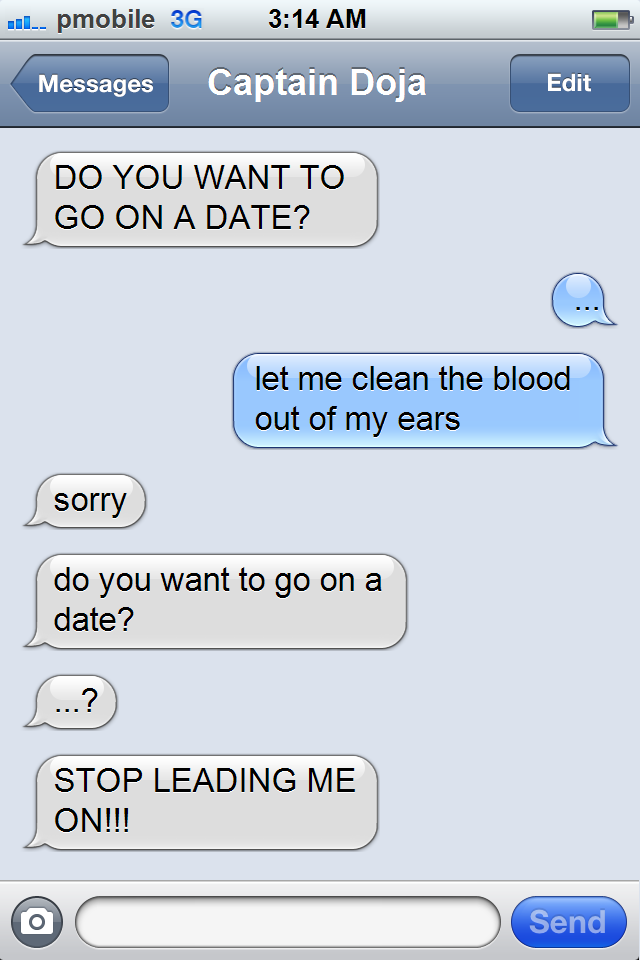
\includegraphics[width=0.5\linewidth]{images/datetext} 

}

\caption{Like a text message, you should probably watch your use of capitalization in R.}\label{fig:datetext}
\end{figure}

Like English, R is case-sensitive -- it R treats capital letters
differently from lower-case letters. For example, the four following
objects \texttt{Plunder}, \texttt{plunder} and \texttt{PLUNDER} are
totally different objects in R:

\begin{Shaded}
\begin{Highlighting}[]
\CommentTok{# These are all different objects}
\NormalTok{Plunder <-}\StringTok{ }\DecValTok{1}
\NormalTok{plunder <-}\StringTok{ }\DecValTok{100}
\NormalTok{PLUNDER <-}\StringTok{ }\DecValTok{5}
\end{Highlighting}
\end{Shaded}

I try to avoid using too many capital letters in object names because
they require me to hold the shift key. This may sound silly, but you'd
be surprised how much easier it is to type \texttt{mydata} than
\texttt{MyData} 100 times.

\subsection{Example: Pirates of The
Caribbean}\label{example-pirates-of-the-caribbean}

Let's do a more practical example -- we'll define an object called
\texttt{blackpearl.usd} which has the global revenue of Pirates of the
Caribbean: Curse of the Black Pearl in U.S. dollars. A quick Google
search showed me that the revenue was \$634,954,103. I'll create the new
object using assignment:

\begin{Shaded}
\begin{Highlighting}[]
\NormalTok{blackpearl.usd <-}\StringTok{ }\DecValTok{634954103}
\end{Highlighting}
\end{Shaded}

Now, my fellow European pirates might want to know how much this is in
Euros. Let's create a new object called \texttt{\{blackpearl.eur} which
converts our original value to Euros by multiplying the original amount
by 0.88 (assuming 1 USD = 0.88 EUR)

\begin{Shaded}
\begin{Highlighting}[]
\NormalTok{blackpearl.eur <-}\StringTok{ }\NormalTok{blackpearl.usd }\OperatorTok{*}\StringTok{ }\FloatTok{0.88}
\NormalTok{blackpearl.eur}
\NormalTok{## [1] 5.6e+08}
\end{Highlighting}
\end{Shaded}

It looks like the movie made 558,759,611 in Euros. Not bad. Now, let's
see how much more Pirates of the Caribbean 2: Dead Man's Chest made
compared to ``Curse of the Black Pearl.'' Another Google search
uncovered that Dead Man's Chest made \$1,066,215,812 (that wasn't a
mistype, the freaking movie made over a billion dollars).

\begin{Shaded}
\begin{Highlighting}[]
\NormalTok{deadman.usd <-}\StringTok{ }\DecValTok{1066215812}
\end{Highlighting}
\end{Shaded}

Now, I'll divide \texttt{deadman.usd} by \texttt{blackpearl.usd}:

\begin{Shaded}
\begin{Highlighting}[]
\NormalTok{deadman.usd }\OperatorTok{/}\StringTok{ }\NormalTok{blackpearl.usd}
\NormalTok{## [1] 1.7}
\end{Highlighting}
\end{Shaded}

It looks like ``Dead Man's Chest'' made 168\% as much as ``Curse of the
Black Pearl'' - not bad for two movies based off of a ride from
Disneyland.

\section{Test your R might!}\label{test-your-r-might}

\begin{enumerate}
\def\labelenumi{\arabic{enumi}.}
\item
  Create a new R script. Using comments, write your name, the date, and
  ``Testing my Chapter 2 R Might'' at the top of the script. Write your
  answers to the rest of these exercises on this script, and be sure to
  copy and paste the original questions using comments! Your script
  should \textbf{only} contain valid R code and comments.
\item
  Which (if any) of the following objects names is/are invalid?
\end{enumerate}

\begin{Shaded}
\begin{Highlighting}[]
\NormalTok{thisone <-}\StringTok{ }\DecValTok{1}
\NormalTok{THISONE <-}\StringTok{ }\DecValTok{2}
\NormalTok{1This <-}\StringTok{ }\DecValTok{3}
\NormalTok{this.one <-}\StringTok{ }\DecValTok{4}
\NormalTok{This.}\DecValTok{1}\NormalTok{ <-}\StringTok{ }\DecValTok{5}
\NormalTok{ThIS.....ON...E <-}\StringTok{ }\DecValTok{6}
\NormalTok{This}\OperatorTok{!}\NormalTok{On}\OperatorTok{!}\NormalTok{e <-}\StringTok{ }\DecValTok{7}
\NormalTok{lkjasdfkjsdf <-}\StringTok{ }\DecValTok{8}
\end{Highlighting}
\end{Shaded}

\begin{enumerate}
\def\labelenumi{\arabic{enumi}.}
\setcounter{enumi}{2}
\item
  2015 was a good year for pirate booty - your ship collected 100,800
  gold coins. Create an object called \texttt{gold.in.2015} and assign
  the correct value to it.
\item
  Oops, during the last inspection we discovered that one of your
  pirates Skippy McGee hid 800 gold coins in his underwear. Go ahead and
  add those gold coins to the object \texttt{gold.in.2015}. Next, create
  an object called \texttt{plank.list} with the name of the pirate
  thief.
\item
  Look at the code below. What will R return after the third line? Make
  a prediction, then test the code yourself.
\end{enumerate}

\begin{Shaded}
\begin{Highlighting}[]
\NormalTok{a <-}\StringTok{ }\DecValTok{10}
\NormalTok{a }\OperatorTok{+}\StringTok{ }\DecValTok{10}
\NormalTok{a}
\end{Highlighting}
\end{Shaded}

\chapter{Scalars and vectors}\label{scalersvectors}

\begin{figure}

{\centering 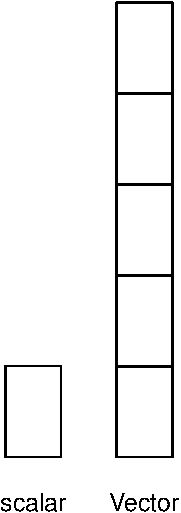
\includegraphics{YaRrr_files/figure-latex/scalervector-1} 

}

\caption{Visual depiction of a scalar and vector. Deep shit. Wait until we get to matrices - you're going to lose it.}\label{fig:scalervector}
\end{figure}

\begin{Shaded}
\begin{Highlighting}[]
\CommentTok{# Crew information}
\NormalTok{captain.name <-}\StringTok{ "Jack"}
\NormalTok{captain.age <-}\StringTok{ }\DecValTok{33}

\NormalTok{crew.names <-}\StringTok{ }\KeywordTok{c}\NormalTok{(}\StringTok{"Heath"}\NormalTok{, }\StringTok{"Vincent"}\NormalTok{, }\StringTok{"Maya"}\NormalTok{, }\StringTok{"Becki"}\NormalTok{)}
\NormalTok{crew.ages <-}\StringTok{ }\KeywordTok{c}\NormalTok{(}\DecValTok{19}\NormalTok{, }\DecValTok{35}\NormalTok{, }\DecValTok{22}\NormalTok{, }\DecValTok{44}\NormalTok{)}
\NormalTok{crew.sex <-}\StringTok{ }\KeywordTok{c}\NormalTok{(}\KeywordTok{rep}\NormalTok{(}\StringTok{"M"}\NormalTok{, }\DataTypeTok{times =} \DecValTok{2}\NormalTok{), }\KeywordTok{rep}\NormalTok{(}\StringTok{"F"}\NormalTok{, }\DataTypeTok{times =} \DecValTok{2}\NormalTok{))}
\NormalTok{crew.ages.decade <-}\StringTok{ }\NormalTok{crew.ages }\OperatorTok{/}\StringTok{ }\DecValTok{10}

\CommentTok{# Earnings over first 10 days at sea}
\NormalTok{days <-}\StringTok{ }\DecValTok{1}\OperatorTok{:}\DecValTok{10}
\NormalTok{gold <-}\StringTok{ }\KeywordTok{seq}\NormalTok{(}\DataTypeTok{from =} \DecValTok{10}\NormalTok{, }\DataTypeTok{to =} \DecValTok{100}\NormalTok{, }\DataTypeTok{by =} \DecValTok{10}\NormalTok{)}
\NormalTok{silver <-}\StringTok{ }\KeywordTok{rep}\NormalTok{(}\DecValTok{50}\NormalTok{, }\DataTypeTok{times =} \DecValTok{10}\NormalTok{)}
\NormalTok{total <-}\StringTok{ }\NormalTok{gold }\OperatorTok{+}\StringTok{ }\NormalTok{silver}
\end{Highlighting}
\end{Shaded}

People are not objects. But R is full of them. Here are some of the
basic ones.

\section{Scalars}\label{scalars}

The simplest object type in R is a \textbf{scalar}. A scalar object is
just a single value like a number or a name. In the previous chapter we
defined several scalar objects. Here are examples of numeric scalars:

\begin{Shaded}
\begin{Highlighting}[]
\CommentTok{# Examples of numeric scalers}
\NormalTok{a <-}\StringTok{ }\DecValTok{100}
\NormalTok{b <-}\StringTok{ }\DecValTok{3} \OperatorTok{/}\StringTok{ }\DecValTok{100}
\NormalTok{c <-}\StringTok{ }\NormalTok{(a }\OperatorTok{+}\StringTok{ }\NormalTok{b) }\OperatorTok{/}\StringTok{ }\NormalTok{b}
\end{Highlighting}
\end{Shaded}

Scalars don't have to be numeric, they can also be \textbf{characters}
(also known as strings). In R, you denote characters using quotation
marks. Here are examples of character scalars:

\begin{Shaded}
\begin{Highlighting}[]
\CommentTok{# Examples of character scalers}
\NormalTok{d <-}\StringTok{ "ship"}
\NormalTok{e <-}\StringTok{ "cannon"}
\NormalTok{f <-}\StringTok{ "Do any modern armies still use cannons?"}
\end{Highlighting}
\end{Shaded}

As you can imagine, R treats numeric and character scalars differently.
For example, while you can do basic arithmetic operations on numeric
scalars -- they won't work on character scalars. If you try to perform
numeric operations (like addition) on character scalars, you'll get an
error like this one:

\begin{Shaded}
\begin{Highlighting}[]
\NormalTok{a <-}\StringTok{ "1"}
\NormalTok{b <-}\StringTok{ "2"}
\NormalTok{a }\OperatorTok{+}\StringTok{ }\NormalTok{b}
\end{Highlighting}
\end{Shaded}

Error in a + b: non-numeric argument to binary operator

If you see an error like this one, it means that you're trying to apply
numeric operations to character objects. That's just sick and wrong.

\section{Vectors}\label{vectors}

Now let's move onto \texttt{vectors}. A vector object is just a
combination of several scalars stored as a single object. For example,
the numbers from one to ten could be a vector of length 10, and the
characters in the English alphabet could be a vector of length 26. Like
scalars, vectors can be either numeric or character (but not both!).

There are many ways to create vectors in R. Here are the methods we will
cover in this chapter:

\begin{longtable}[]{@{}lll@{}}
\caption{Functions to create vectors.}\tabularnewline
\toprule
\begin{minipage}[b]{0.34\columnwidth}\raggedright\strut
Function\strut
\end{minipage} & \begin{minipage}[b]{0.39\columnwidth}\raggedright\strut
Example\strut
\end{minipage} & \begin{minipage}[b]{0.15\columnwidth}\raggedright\strut
Result\strut
\end{minipage}\tabularnewline
\midrule
\endfirsthead
\toprule
\begin{minipage}[b]{0.34\columnwidth}\raggedright\strut
Function\strut
\end{minipage} & \begin{minipage}[b]{0.39\columnwidth}\raggedright\strut
Example\strut
\end{minipage} & \begin{minipage}[b]{0.15\columnwidth}\raggedright\strut
Result\strut
\end{minipage}\tabularnewline
\midrule
\endhead
\begin{minipage}[t]{0.34\columnwidth}\raggedright\strut
\texttt{c(a,\ b,\ ...)}\strut
\end{minipage} & \begin{minipage}[t]{0.39\columnwidth}\raggedright\strut
\texttt{c(1,\ 5,\ 9)}\strut
\end{minipage} & \begin{minipage}[t]{0.15\columnwidth}\raggedright\strut
1, 5, 9\strut
\end{minipage}\tabularnewline
\begin{minipage}[t]{0.34\columnwidth}\raggedright\strut
\texttt{a:b}\strut
\end{minipage} & \begin{minipage}[t]{0.39\columnwidth}\raggedright\strut
\texttt{1:5}\strut
\end{minipage} & \begin{minipage}[t]{0.15\columnwidth}\raggedright\strut
1, 2, 3, 4, 5\strut
\end{minipage}\tabularnewline
\begin{minipage}[t]{0.34\columnwidth}\raggedright\strut
\texttt{seq(from,\ to,\ by,\ length.out)}\strut
\end{minipage} & \begin{minipage}[t]{0.39\columnwidth}\raggedright\strut
\texttt{seq(from\ =\ 0,\ to\ =\ 6,\ by\ =\ 2)}\strut
\end{minipage} & \begin{minipage}[t]{0.15\columnwidth}\raggedright\strut
0, 2, 4, 6\strut
\end{minipage}\tabularnewline
\begin{minipage}[t]{0.34\columnwidth}\raggedright\strut
\texttt{rep(x,\ times,\ each,\ length.out)}\strut
\end{minipage} & \begin{minipage}[t]{0.39\columnwidth}\raggedright\strut
\texttt{rep(c(7,\ 8),\ times\ =\ 2,\ each\ =\ 2)}\strut
\end{minipage} & \begin{minipage}[t]{0.15\columnwidth}\raggedright\strut
7, 7, 8, 8, 7, 7, 8, 8\strut
\end{minipage}\tabularnewline
\bottomrule
\end{longtable}

The simplest way to create a vector is with the \texttt{c()} function.
The c here stands for concatenate, which means ``bring them together''.
The \texttt{c()} function takes several scalars as arguments, and
returns a vector containing those objects. When using c(), place a comma
in between the objects (scalars or vectors) you want to combine:

Let's use the \texttt{c()} function to create a vector called \texttt{a}
containing the integers from 1 to 5.

\begin{Shaded}
\begin{Highlighting}[]
\CommentTok{# Create an object a with the integers from 1 to 5}
\NormalTok{a <-}\StringTok{ }\KeywordTok{c}\NormalTok{(}\DecValTok{1}\NormalTok{, }\DecValTok{2}\NormalTok{, }\DecValTok{3}\NormalTok{, }\DecValTok{4}\NormalTok{, }\DecValTok{5}\NormalTok{)}

\CommentTok{# Print the result}
\NormalTok{a}
\NormalTok{## [1] 1 2 3 4 5}
\end{Highlighting}
\end{Shaded}

As you can see, R has stored all 5 numbers in the object \texttt{a}.
Thanks R!

You can also create longer vectors by combining vectors you have already
defined. Let's create a vector of the numbers from 1 to 10 by first
generating a vector \texttt{a} from 1 to 5, and a vector \texttt{b} from
6 to 10 then combine them into a single vector \texttt{x}:

\begin{Shaded}
\begin{Highlighting}[]
\NormalTok{a <-}\StringTok{ }\KeywordTok{c}\NormalTok{(}\DecValTok{1}\NormalTok{, }\DecValTok{2}\NormalTok{, }\DecValTok{3}\NormalTok{, }\DecValTok{4}\NormalTok{, }\DecValTok{5}\NormalTok{)}
\NormalTok{b <-}\StringTok{ }\KeywordTok{c}\NormalTok{(}\DecValTok{6}\NormalTok{, }\DecValTok{7}\NormalTok{, }\DecValTok{8}\NormalTok{, }\DecValTok{9}\NormalTok{, }\DecValTok{10}\NormalTok{)}
\NormalTok{x <-}\StringTok{ }\KeywordTok{c}\NormalTok{(a, b)}
\NormalTok{x}
\NormalTok{##  [1]  1  2  3  4  5  6  7  8  9 10}
\end{Highlighting}
\end{Shaded}

You can also create character vectors by using the \texttt{c()} function
to combine character scalars into character vectors:

\begin{figure}

{\centering 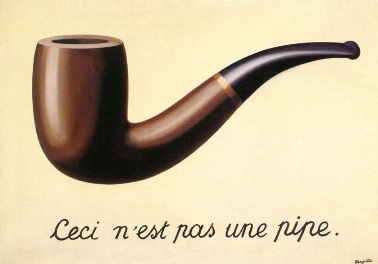
\includegraphics[width=0.5\linewidth]{images/magrittepipe} 

}

\caption{This is not a pipe. It is a character vector.}\label{fig:unnamed-chunk-86}
\end{figure}

\begin{Shaded}
\begin{Highlighting}[]
\NormalTok{char.vec <-}\StringTok{ }\KeywordTok{c}\NormalTok{(}\StringTok{"Ceci"}\NormalTok{, }\StringTok{"nest"}\NormalTok{, }\StringTok{"pas"}\NormalTok{, }\StringTok{"une"}\NormalTok{, }\StringTok{"pipe"}\NormalTok{)}
\NormalTok{char.vec}
\NormalTok{## [1] "Ceci" "nest" "pas"  "une"  "pipe"}
\end{Highlighting}
\end{Shaded}

While the \texttt{c()} function is the most straightforward way to
create a vector, it's also one of the most tedious. For example, let's
say you wanted to create a vector of all integers from 1 to 100. You
definitely don't want to have to type all the numbers into a c()
operator. Thankfully, R has many simple built-in functions for
generating numeric vectors. Let's start with three of them:
\texttt{a:b}, \texttt{seq()}, and \texttt{rep()}:

\subsection{a:b}\label{ab}

The \texttt{a:b} function takes two numeric scalars \texttt{a} and
\texttt{b} as arguments, and returns a vector of numbers from the
starting point \texttt{a} to the ending point \texttt{b} in steps of 1.

Here are some examples of the \texttt{a:b} function in action. As you'll
see, you can go backwards or forwards, or make sequences between
non-integers:

\begin{Shaded}
\begin{Highlighting}[]
\DecValTok{1}\OperatorTok{:}\DecValTok{10}
\NormalTok{##  [1]  1  2  3  4  5  6  7  8  9 10}
\DecValTok{10}\OperatorTok{:}\DecValTok{1}
\NormalTok{##  [1] 10  9  8  7  6  5  4  3  2  1}
\FloatTok{2.5}\OperatorTok{:}\FloatTok{8.5}
\NormalTok{## [1] 2.5 3.5 4.5 5.5 6.5 7.5 8.5}
\end{Highlighting}
\end{Shaded}

\subsection{seq()}\label{seq}

\begin{longtable}[]{@{}ll@{}}
\toprule
\begin{minipage}[b]{0.35\columnwidth}\raggedright\strut
Argument\strut
\end{minipage} & \begin{minipage}[b]{0.41\columnwidth}\raggedright\strut
Definition\strut
\end{minipage}\tabularnewline
\midrule
\endhead
\begin{minipage}[t]{0.35\columnwidth}\raggedright\strut
\texttt{from}\strut
\end{minipage} & \begin{minipage}[t]{0.41\columnwidth}\raggedright\strut
The start of the sequence\strut
\end{minipage}\tabularnewline
\begin{minipage}[t]{0.35\columnwidth}\raggedright\strut
\texttt{to}\strut
\end{minipage} & \begin{minipage}[t]{0.41\columnwidth}\raggedright\strut
The end of the sequence\strut
\end{minipage}\tabularnewline
\begin{minipage}[t]{0.35\columnwidth}\raggedright\strut
\texttt{by}\strut
\end{minipage} & \begin{minipage}[t]{0.41\columnwidth}\raggedright\strut
The step-size of the sequence\strut
\end{minipage}\tabularnewline
\begin{minipage}[t]{0.35\columnwidth}\raggedright\strut
\texttt{length.out}\strut
\end{minipage} & \begin{minipage}[t]{0.41\columnwidth}\raggedright\strut
The desired length of the final sequence (only use if you don't specify
\texttt{by})\strut
\end{minipage}\tabularnewline
\bottomrule
\end{longtable}

The \texttt{seq()} function is a more flexible version of \texttt{a:b}.
Like \texttt{a:b}, \texttt{seq()} allows you to create a sequence from a
starting number to an ending number. However, \texttt{seq()}, has
additional arguments that allow you to specify either the size of the
steps between numbers, or the total length of the sequence:

The \texttt{seq()} function has two new arguments \texttt{by} and
\texttt{length.out}. If you use the \texttt{by} argument, the sequence
will be in steps of the input to the \texttt{by} argument:

\begin{Shaded}
\begin{Highlighting}[]
\CommentTok{# Create the numbers from 1 to 10 in steps of 1}
\KeywordTok{seq}\NormalTok{(}\DataTypeTok{from =} \DecValTok{1}\NormalTok{, }\DataTypeTok{to =} \DecValTok{10}\NormalTok{, }\DataTypeTok{by =} \DecValTok{1}\NormalTok{)}
\NormalTok{##  [1]  1  2  3  4  5  6  7  8  9 10}

\CommentTok{# Integers from 0 to 100 in steps of 10}
\KeywordTok{seq}\NormalTok{(}\DataTypeTok{from =} \DecValTok{0}\NormalTok{, }\DataTypeTok{to =} \DecValTok{100}\NormalTok{, }\DataTypeTok{by =} \DecValTok{10}\NormalTok{)}
\NormalTok{##  [1]   0  10  20  30  40  50  60  70  80  90 100}
\end{Highlighting}
\end{Shaded}

If you use the \texttt{length.out} argument, the sequence will have
length equal to \texttt{length.out}.

\begin{Shaded}
\begin{Highlighting}[]
\CommentTok{# Create 10 numbers from 1 to 5}
\KeywordTok{seq}\NormalTok{(}\DataTypeTok{from =} \DecValTok{1}\NormalTok{, }\DataTypeTok{to =} \DecValTok{5}\NormalTok{, }\DataTypeTok{length.out =} \DecValTok{10}\NormalTok{)}
\NormalTok{##  [1] 1.0 1.4 1.9 2.3 2.8 3.2 3.7 4.1 4.6 5.0}

\CommentTok{# 3 numbers from 0 to 100}
\KeywordTok{seq}\NormalTok{(}\DataTypeTok{from =} \DecValTok{0}\NormalTok{, }\DataTypeTok{to =} \DecValTok{100}\NormalTok{, }\DataTypeTok{length.out =} \DecValTok{3}\NormalTok{)}
\NormalTok{## [1]   0  50 100}
\end{Highlighting}
\end{Shaded}

\subsection{rep()}\label{rep}

\begin{longtable}[]{@{}ll@{}}
\toprule
Argument & Definition\tabularnewline
\midrule
\endhead
\texttt{x} & A scalar or vector of values to repeat\tabularnewline
\texttt{times} & The number of times to repeat x\tabularnewline
\texttt{each} & The number of times to repeat each value within
x\tabularnewline
\texttt{length.out} & The desired length of the final
sequence\tabularnewline
\bottomrule
\end{longtable}

\begin{figure}

{\centering 
\includegraphics[width=0.5\linewidth]{images/rep} 

}

\caption{Not a good depiction of a rep in R.}\label{fig:rep}
\end{figure}

The \texttt{rep()} function allows you to repeat a scalar (or vector) a
specified number of times, or to a desired length. Let's do some reps.

\begin{Shaded}
\begin{Highlighting}[]
\KeywordTok{rep}\NormalTok{(}\DataTypeTok{x =} \DecValTok{3}\NormalTok{, }\DataTypeTok{times =} \DecValTok{10}\NormalTok{)}
\NormalTok{##  [1] 3 3 3 3 3 3 3 3 3 3}
\KeywordTok{rep}\NormalTok{(}\DataTypeTok{x =} \KeywordTok{c}\NormalTok{(}\DecValTok{1}\NormalTok{, }\DecValTok{2}\NormalTok{), }\DataTypeTok{each =} \DecValTok{3}\NormalTok{)}
\NormalTok{## [1] 1 1 1 2 2 2}
\KeywordTok{rep}\NormalTok{(}\DataTypeTok{x =} \DecValTok{1}\OperatorTok{:}\DecValTok{3}\NormalTok{, }\DataTypeTok{length.out =} \DecValTok{10}\NormalTok{)}
\NormalTok{##  [1] 1 2 3 1 2 3 1 2 3 1}
\end{Highlighting}
\end{Shaded}

As you can see, you can can include an \texttt{a:b} call within a
\texttt{rep()}!

You can even combine the \texttt{times} and \texttt{each} arguments
within a single \texttt{rep()} function. For example, here's how to
create the sequence \{1, 1, 2, 2, 3, 3, 1, 1, 2, 2, 3, 3\} with one call
to \texttt{rep()}:

\begin{Shaded}
\begin{Highlighting}[]
\KeywordTok{rep}\NormalTok{(}\DataTypeTok{x =} \DecValTok{1}\OperatorTok{:}\DecValTok{3}\NormalTok{, }\DataTypeTok{each =} \DecValTok{2}\NormalTok{, }\DataTypeTok{times =} \DecValTok{2}\NormalTok{)}
\NormalTok{##  [1] 1 1 2 2 3 3 1 1 2 2 3 3}
\end{Highlighting}
\end{Shaded}

\textbf{Warning! Vectors contain either numbers or characters, not both}

A vector can only contain one type of scalar: either numeric or
character. If you try to create a vector with numeric and character
scalars, then R will convert \emph{all} of the numeric scalars to
characters. In the next code chunk, I'll create a new vector called
\texttt{my.vec} that contains a mixture of numeric and character
scalars.

\begin{Shaded}
\begin{Highlighting}[]
\NormalTok{my.vec <-}\StringTok{ }\KeywordTok{c}\NormalTok{(}\StringTok{"a"}\NormalTok{, }\DecValTok{1}\NormalTok{, }\StringTok{"b"}\NormalTok{, }\DecValTok{2}\NormalTok{, }\StringTok{"c"}\NormalTok{, }\DecValTok{3}\NormalTok{)}
\NormalTok{my.vec}
\NormalTok{## [1] "a" "1" "b" "2" "c" "3"}
\end{Highlighting}
\end{Shaded}

As you can see from the output, \texttt{my.vec} is stored as a character
vector where all the numbers are converted to characters.

\section{Generating random data}\label{generating-random-data}

Because R is a language built for statistics, it contains many functions
that allow you generate random data -- either from a vector of data that
you specify (like Heads or Tails from a coin), or from an established
\emph{probability distribution}, like the Normal or Uniform
distribution.

In the next section we'll go over the standard \texttt{sample()}
function for drawing random values from a vector. We'll then cover some
of the most commonly used probability distributions: Normal and Uniform.

\subsection{sample()}\label{sample}

\begin{longtable}[]{@{}ll@{}}
\toprule
\begin{minipage}[b]{0.14\columnwidth}\raggedright\strut
Argument\strut
\end{minipage} & \begin{minipage}[b]{0.61\columnwidth}\raggedright\strut
Definition\strut
\end{minipage}\tabularnewline
\midrule
\endhead
\begin{minipage}[t]{0.14\columnwidth}\raggedright\strut
\texttt{x}\strut
\end{minipage} & \begin{minipage}[t]{0.61\columnwidth}\raggedright\strut
A vector of outcomes you want to sample from. For example, to simulate
coin flips, you'd enter \texttt{x\ =\ c("H",\ "T")}\strut
\end{minipage}\tabularnewline
\begin{minipage}[t]{0.14\columnwidth}\raggedright\strut
\texttt{size}\strut
\end{minipage} & \begin{minipage}[t]{0.61\columnwidth}\raggedright\strut
The number of samples you want to draw. The default is the length of
\texttt{x}.\strut
\end{minipage}\tabularnewline
\begin{minipage}[t]{0.14\columnwidth}\raggedright\strut
\texttt{replace}\strut
\end{minipage} & \begin{minipage}[t]{0.61\columnwidth}\raggedright\strut
Should sampling be done with replacement? If FALSE (the default value),
then each outcome in \texttt{x} can only be drawn once. If TRUE, then
each outcome in \texttt{x} can be drawn multiple times.\strut
\end{minipage}\tabularnewline
\begin{minipage}[t]{0.14\columnwidth}\raggedright\strut
\texttt{prob}\strut
\end{minipage} & \begin{minipage}[t]{0.61\columnwidth}\raggedright\strut
A vector of probabilities of the same length as \texttt{x} indicating
how likely each outcome in \texttt{x} is. The vector of probabilities
you give as an argument should add up to one. If you don't specify the
\texttt{prob} argument, all outcomes will be equally likely.\strut
\end{minipage}\tabularnewline
\bottomrule
\end{longtable}

The \texttt{sample()} function allows you to draw random samples of
elements (scalars) from a vector. For example, if you want to simulate
the 100 flips of a fair coin, you can tell the sample function to sample
100 values from the vector {[}``Heads'', ``Tails''{]}. Or, if you need
to randomly assign people to either a ``Control'' or ``Test'' condition
in an experiment, you can randomly sample values from the vector
{[}``Control'', ``Test''{]}:

Let's use \texttt{sample()} to draw 10 samples from a vector of integers
from 1 to 10.

\begin{Shaded}
\begin{Highlighting}[]
\CommentTok{# From the integers 1:10, draw 5 numbers}
\KeywordTok{sample}\NormalTok{(}\DataTypeTok{x =} \DecValTok{1}\OperatorTok{:}\DecValTok{10}\NormalTok{, }\DataTypeTok{size  =} \DecValTok{5}\NormalTok{)}
\NormalTok{## [1] 2 1 5 3 9}
\end{Highlighting}
\end{Shaded}

\subsubsection{replace = TRUE}\label{replace-true}

If you don't specify the \texttt{replace} argument, R will assume that
you are sampling \emph{without} replacement. In other words, each
element can only be sampled once. If you want to sample with
replacement, use the \texttt{replace\ =\ TRUE} argument:

Think about replacement like drawing balls from a bag. Sampling
\emph{with} replacement (\texttt{replace\ =\ TRUE}) means that each time
you draw a ball, you return the ball back into the bag before drawing
another ball. Sampling \emph{without} replacement
(\texttt{replace\ =\ FALSE}) means that after you draw a ball, you
remove that ball from the bag so you can never draw it again.

\begin{Shaded}
\begin{Highlighting}[]
\CommentTok{# Draw 30 samples from the integers 1:5 with replacement}
\KeywordTok{sample}\NormalTok{(}\DataTypeTok{x =} \DecValTok{1}\OperatorTok{:}\DecValTok{5}\NormalTok{, }\DataTypeTok{size =} \DecValTok{10}\NormalTok{, }\DataTypeTok{replace =} \OtherTok{TRUE}\NormalTok{)}
\NormalTok{##  [1] 2 3 5 2 3 5 4 4 2 1}
\end{Highlighting}
\end{Shaded}

If you try to draw a large sample from a vector \textit{without}
replacement, R will return an error because it runs out of things to
draw:

\begin{Shaded}
\begin{Highlighting}[]
\CommentTok{# You CAN'T draw 10 samples without replacement from}
\CommentTok{#  a vector with length 5}
\KeywordTok{sample}\NormalTok{(}\DataTypeTok{x =} \DecValTok{1}\OperatorTok{:}\DecValTok{5}\NormalTok{, }\DataTypeTok{size =} \DecValTok{10}\NormalTok{)}
\end{Highlighting}
\end{Shaded}

Error: cannot take a sample larger than the population when `replace =
FALSE'

To fix this, just tell R that you want to sample with replacement:

\begin{Shaded}
\begin{Highlighting}[]
\CommentTok{# You CAN draw 10 samples with replacement from a}
\CommentTok{#  vector of length 5}
\KeywordTok{sample}\NormalTok{(}\DataTypeTok{x =} \DecValTok{1}\OperatorTok{:}\DecValTok{5}\NormalTok{, }\DataTypeTok{size =} \DecValTok{10}\NormalTok{, }\DataTypeTok{replace =} \OtherTok{TRUE}\NormalTok{)}
\NormalTok{##  [1] 4 2 2 3 3 4 5 3 2 5}
\end{Highlighting}
\end{Shaded}

To specify how likely each element in the vector \texttt{x} should be
selected, use the \texttt{prob} argument. The length of the
\texttt{prob} argument should be as long as the \texttt{x} argument. For
example, let's draw 10 samples (with replacement) from the vector
{[}``a'', ``b''{]}, but we'll make the probability of selecting ``a'' to
be .90, and the probability of selecting ``b'' to be .10

\begin{Shaded}
\begin{Highlighting}[]
\KeywordTok{sample}\NormalTok{(}\DataTypeTok{x =} \KeywordTok{c}\NormalTok{(}\StringTok{"a"}\NormalTok{, }\StringTok{"b"}\NormalTok{), }
       \DataTypeTok{prob =} \KeywordTok{c}\NormalTok{(.}\DecValTok{9}\NormalTok{, .}\DecValTok{1}\NormalTok{),}
       \DataTypeTok{size =} \DecValTok{10}\NormalTok{, }
       \DataTypeTok{replace =} \OtherTok{TRUE}\NormalTok{)}
\NormalTok{##  [1] "a" "a" "a" "a" "a" "a" "a" "a" "a" "a"}
\end{Highlighting}
\end{Shaded}

\subsubsection{Ex: Simulating coin
flips}\label{ex-simulating-coin-flips}

Let's simulate 10 flips of a fair coin, were the probably of getting
either a Head or Tail is .50. Because all values are equally likely, we
don't need to specify the \texttt{prob} argument

\begin{Shaded}
\begin{Highlighting}[]
\KeywordTok{sample}\NormalTok{(}\DataTypeTok{x =} \KeywordTok{c}\NormalTok{(}\StringTok{"H"}\NormalTok{, }\StringTok{"T"}\NormalTok{), }\CommentTok{# The possible values of the coin}
       \DataTypeTok{size =} \DecValTok{10}\NormalTok{,  }\CommentTok{# 10 flips}
       \DataTypeTok{replace =} \OtherTok{TRUE}\NormalTok{) }\CommentTok{# Sampling with replacement}
\NormalTok{##  [1] "H" "H" "T" "T" "H" "T" "H" "T" "H" "H"}
\end{Highlighting}
\end{Shaded}

Now let's change it by simulating flips of a biased coin, where the
probability of Heads is 0.8, and the probability of Tails is 0.2.
Because the probabilities of each outcome are no longer equal, we'll
need to specify them with the \texttt{prob} argument:

\begin{Shaded}
\begin{Highlighting}[]
\KeywordTok{sample}\NormalTok{(}\DataTypeTok{x =} \KeywordTok{c}\NormalTok{(}\StringTok{"H"}\NormalTok{, }\StringTok{"T"}\NormalTok{),}
       \DataTypeTok{prob =} \KeywordTok{c}\NormalTok{(.}\DecValTok{8}\NormalTok{, .}\DecValTok{2}\NormalTok{), }\CommentTok{# Make the coin biased for Heads}
       \DataTypeTok{size =} \DecValTok{10}\NormalTok{,}
       \DataTypeTok{replace =} \OtherTok{TRUE}\NormalTok{)}
\NormalTok{##  [1] "H" "H" "H" "H" "H" "T" "T" "H" "H" "H"}
\end{Highlighting}
\end{Shaded}

As you can see, our function returned a vector of 10 values
corresponding to our sample size of 10.

\subsubsection{Ex: Coins from a chest}\label{ex-coins-from-a-chest}

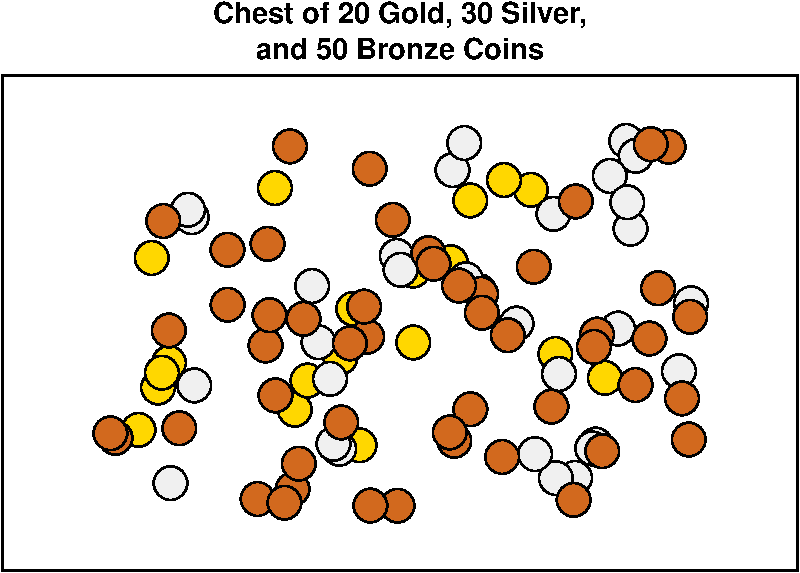
\includegraphics{YaRrr_files/figure-latex/unnamed-chunk-101-1.pdf}

Now, let's sample drawing coins from a treasure chest Let's say the
chest has 100 coins: 20 gold, 30 silver, and 50 bronze. Let's draw 10
random coins from this chest.

\begin{Shaded}
\begin{Highlighting}[]
\CommentTok{# Create chest with the 100 coins}

\NormalTok{chest <-}\StringTok{ }\KeywordTok{c}\NormalTok{(}\KeywordTok{rep}\NormalTok{(}\StringTok{"gold"}\NormalTok{, }\DecValTok{20}\NormalTok{),}
         \KeywordTok{rep}\NormalTok{(}\StringTok{"silver"}\NormalTok{, }\DecValTok{30}\NormalTok{),}
         \KeywordTok{rep}\NormalTok{(}\StringTok{"bronze"}\NormalTok{, }\DecValTok{50}\NormalTok{))}

\CommentTok{# Draw 10 coins from the chest}
\KeywordTok{sample}\NormalTok{(}\DataTypeTok{x =}\NormalTok{ chest,}
       \DataTypeTok{size =} \DecValTok{10}\NormalTok{)}
\NormalTok{##  [1] "bronze" "bronze" "bronze" "bronze" "bronze" "silver" "bronze"}
\NormalTok{##  [8] "bronze" "bronze" "silver"}
\end{Highlighting}
\end{Shaded}

The output of the \texttt{sample()} function above is a vector of 10
strings indicating the type of coin we drew on each sample. And like any
random sampling function, this code will likely give you different
results every time you run it! See how long it takes you to get 10 gold
coins\ldots{}

In the next section, we'll cover how to generate random data from
specified \emph{probability distributions}. What is a probability
distribution? Well, it's simply an equation -- also called a likelihood
function -- that indicates how likely certain numerical values are to be
drawn.

We can use probability distributions to represent different types of
data. For example, imagine you need to hire a new group of pirates for
your crew. You have the option of hiring people from one of two
different pirate training colleges that produce pirates of varying
quality. One college ``Pirate Training Unlimited'' might tend to pirates
that are generally ok - never great but never terrible. While another
college ``Unlimited Pirate Training'' might produce pirates with a wide
variety of quality, from very low to very high. In Figure
\ref{fig:piratecollege} I plotted 5 example pirates from each college,
where each pirate is shown as a ball with a number written on it. As you
can see, pirates from PTU all tend to be clustered between 40 and 60
(not terrible but not great), while pirates from UPT are all over the
map, from 0 to 100. We can use probability distributions (in this case,
the uniform distribution) to mathematically define how likely any
possible value is to be drawn at random from a distribution. We could
describe Pirate Training Unlimited with a uniform distribution with a
small range, and Unlimited Pirate Training with a second uniform
distribution with a wide range.

\begin{figure}
\centering
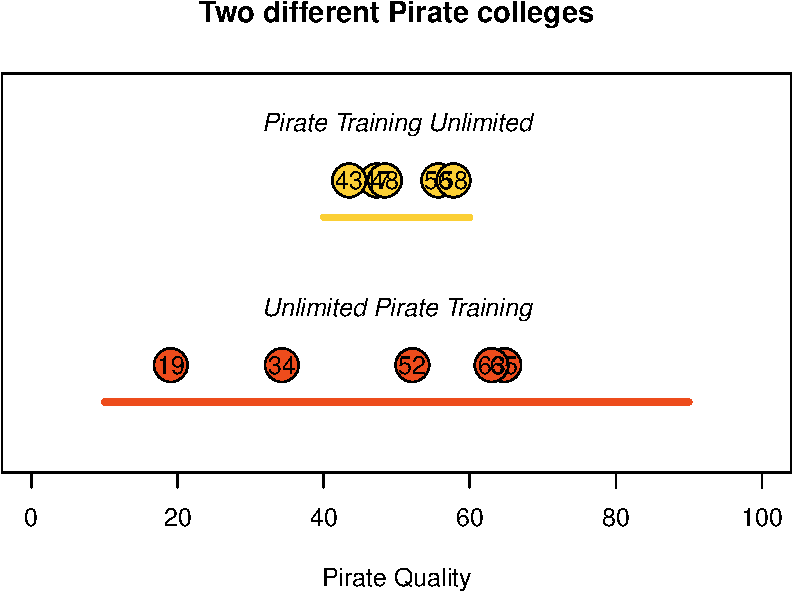
\includegraphics{YaRrr_files/figure-latex/piratecollege-1.pdf}
\caption{\label{fig:piratecollege}Sampling 5 potential pirates from two
different pirate colleges. Pirate Training Unlimited (PTU) consistently
produces average pirates (with scores between 40 and 60), while
Unlimited Pirate Training (UPT), produces a wide range of pirates from 0
to 100.}
\end{figure}

In the next two sections, I'll cover the two most common distributions:
The Normal and the Uniform. However, R contains many more distributions
than just these two. To see them all, look at the help menu for
Distributions:

\begin{Shaded}
\begin{Highlighting}[]
\CommentTok{# See all distributions included in Base R}
\NormalTok{?Distributions}
\end{Highlighting}
\end{Shaded}

\subsection{Normal (Gaussian)}\label{normal-gaussian}

\begin{figure}
\centering
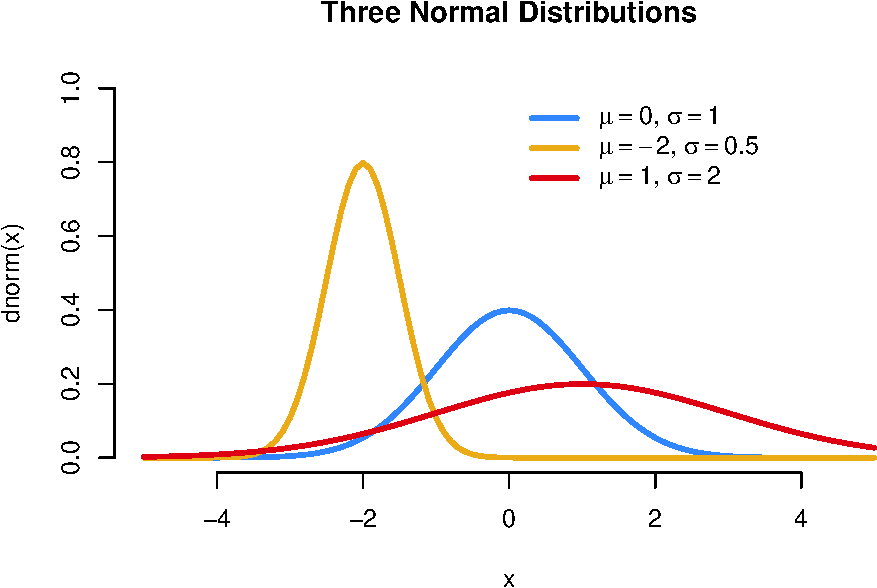
\includegraphics{YaRrr_files/figure-latex/normaldist-1.pdf}
\caption{\label{fig:normaldist}Three different normal distributions with
different means and standard deviations}
\end{figure}

\begin{longtable}[]{@{}ll@{}}
\toprule
Argument & Definition\tabularnewline
\midrule
\endhead
\texttt{n} & The number of observations to draw from the
distribution.\tabularnewline
\texttt{mean} & The mean of the distribution.\tabularnewline
\texttt{sd} & The standard deviation of the distribution.\tabularnewline
\bottomrule
\end{longtable}

The Normal (a.k.a ``Gaussian'') distribution is probably the most
important distribution in all of statistics. The Normal distribution is
bell-shaped, and has two parameters: a mean and a standard deviation. To
generate samples from a normal distribution in R, we use the function
\texttt{rnorm()}

\begin{Shaded}
\begin{Highlighting}[]
\CommentTok{# 5 samples from a Normal dist with mean = 0, sd = 1}
\KeywordTok{rnorm}\NormalTok{(}\DataTypeTok{n =} \DecValTok{5}\NormalTok{, }\DataTypeTok{mean =} \DecValTok{0}\NormalTok{, }\DataTypeTok{sd =} \DecValTok{1}\NormalTok{)}
\NormalTok{## [1] -1.38  2.40  0.37  0.53  0.69}

\CommentTok{# 3 samples from a Normal dist with mean = -10, sd = 15}
\KeywordTok{rnorm}\NormalTok{(}\DataTypeTok{n =} \DecValTok{3}\NormalTok{, }\DataTypeTok{mean =} \OperatorTok{-}\DecValTok{10}\NormalTok{, }\DataTypeTok{sd =} \DecValTok{15}\NormalTok{)}
\NormalTok{## [1] -21 -14 -25}
\end{Highlighting}
\end{Shaded}

Again, because the sampling is done randomly, you'll get different
values each time you run \texttt{rnorm()}

\subsection{Uniform}\label{uniform}

\begin{figure}
\centering
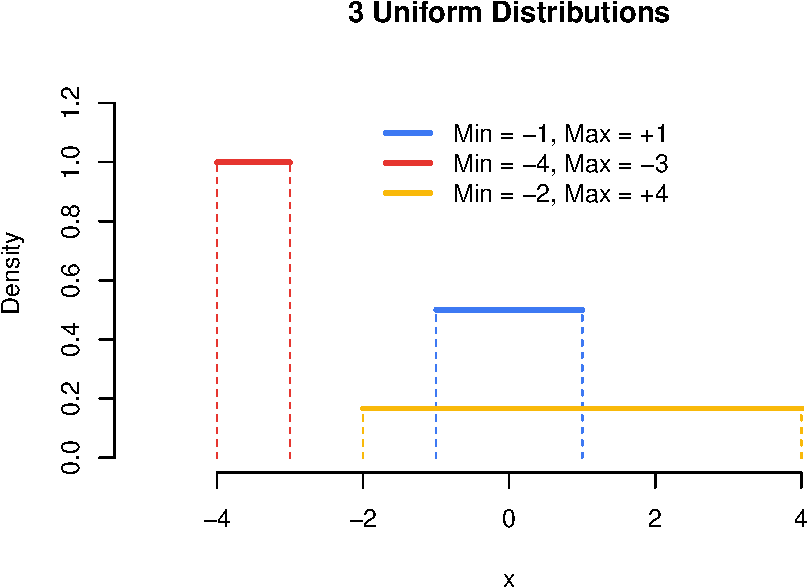
\includegraphics{YaRrr_files/figure-latex/uniformdist-1.pdf}
\caption{\label{fig:uniformdist}The Uniform distribution - known
colloquially as the Anthony Davis distribution.}
\end{figure}

Next, let's move on to the Uniform distribution. The Uniform
distribution gives equal probability to all values between its minimum
and maximum values. In other words, everything between its lower and
upper bounds are equally likely to occur. To generate samples from a
uniform distribution, use the function \texttt{runif()}, the function
has 3 arguments:

\begin{longtable}[]{@{}ll@{}}
\toprule
\begin{minipage}[b]{0.14\columnwidth}\raggedright\strut
Argument\strut
\end{minipage} & \begin{minipage}[b]{0.61\columnwidth}\raggedright\strut
Definition\strut
\end{minipage}\tabularnewline
\midrule
\endhead
\begin{minipage}[t]{0.14\columnwidth}\raggedright\strut
\texttt{n}\strut
\end{minipage} & \begin{minipage}[t]{0.61\columnwidth}\raggedright\strut
The number of observations to draw from the distribution.\strut
\end{minipage}\tabularnewline
\begin{minipage}[t]{0.14\columnwidth}\raggedright\strut
\texttt{min}\strut
\end{minipage} & \begin{minipage}[t]{0.61\columnwidth}\raggedright\strut
The lower bound of the Uniform distribution from which samples are
drawn\strut
\end{minipage}\tabularnewline
\begin{minipage}[t]{0.14\columnwidth}\raggedright\strut
\texttt{max}\strut
\end{minipage} & \begin{minipage}[t]{0.61\columnwidth}\raggedright\strut
The upper bound of the Uniform distribution from which samples are
drawn\strut
\end{minipage}\tabularnewline
\bottomrule
\end{longtable}

Here are some samples from two different Uniform distributions:

\begin{Shaded}
\begin{Highlighting}[]
\CommentTok{# 5 samples from Uniform dist with bounds at 0 and 1}
\KeywordTok{runif}\NormalTok{(}\DataTypeTok{n =} \DecValTok{5}\NormalTok{, }\DataTypeTok{min =} \DecValTok{0}\NormalTok{, }\DataTypeTok{max =} \DecValTok{1}\NormalTok{)}
\NormalTok{## [1] 0.94 0.80 0.57 0.11 0.22}

\CommentTok{# 10 samples from Uniform dist with bounds at -100 and +100}
\KeywordTok{runif}\NormalTok{(}\DataTypeTok{n =} \DecValTok{10}\NormalTok{, }\DataTypeTok{min =} \OperatorTok{-}\DecValTok{100}\NormalTok{, }\DataTypeTok{max =} \DecValTok{100}\NormalTok{)}
\NormalTok{##  [1]  10.94 -80.50  52.38   0.45 -79.65  31.94  87.28 -67.69 -58.64  -0.37}
\end{Highlighting}
\end{Shaded}

\subsection{Notes on random samples}\label{notes-on-random-samples}

\subsubsection{Random samples will always
change}\label{random-samples-will-always-change}

Every time you draw a sample from a probability distribution, you'll
(likely) get a different result. For example, see what happens when I
run the following two commands (you'll learn the \texttt{rnorm()}
function on the next page\ldots{})

\begin{Shaded}
\begin{Highlighting}[]
\CommentTok{# Draw a sample of size 5 from a normal distribution with mean 100 and sd 10}
\KeywordTok{rnorm}\NormalTok{(}\DataTypeTok{n =} \DecValTok{5}\NormalTok{, }\DataTypeTok{mean =} \DecValTok{100}\NormalTok{, }\DataTypeTok{sd =} \DecValTok{10}\NormalTok{)}
\NormalTok{## [1] 107  94 103 106 100}

\CommentTok{# Do it again!}
\KeywordTok{rnorm}\NormalTok{(}\DataTypeTok{n =} \DecValTok{5}\NormalTok{, }\DataTypeTok{mean =} \DecValTok{100}\NormalTok{, }\DataTypeTok{sd =} \DecValTok{10}\NormalTok{)}
\NormalTok{## [1] 113 104 109 108  96}
\end{Highlighting}
\end{Shaded}

As you can see, the exact same code produced different results -- and
that's exactly what we want! Each time you run \texttt{rnorm()}, or
another distribution function, you'll get a new random sample.

\subsubsection{\texorpdfstring{Use \texttt{set.seed()} to control random
samples}{Use set.seed() to control random samples}}\label{use-set.seed-to-control-random-samples}

There will be cases where you will want to exert some control over the
random samples that R produces from sampling functions. For example, you
may want to create a reproducible example of some code that anyone else
can replicate exactly. To do this, use the \texttt{set.seed()} function.
Using \texttt{set.seed()} will force R to produce consistent random
samples at any time on any computer.

In the code below I'll set the sampling seed to 100 with
\texttt{set.seed(100)}. I'll then run \texttt{rnorm()} twice. The
results will always be consistent (because we fixed the sampling seed).

\begin{Shaded}
\begin{Highlighting}[]
\CommentTok{# Fix sampling seed to 100, so the next sampling functions}
\CommentTok{#   always produce the same values}
\KeywordTok{set.seed}\NormalTok{(}\DecValTok{100}\NormalTok{)}

\CommentTok{# The result will always be -0.5022, 0.1315, -0.0789}
\KeywordTok{rnorm}\NormalTok{(}\DecValTok{3}\NormalTok{, }\DataTypeTok{mean =} \DecValTok{0}\NormalTok{, }\DataTypeTok{sd =} \DecValTok{1}\NormalTok{)}
\NormalTok{## [1] -0.502  0.132 -0.079}

\CommentTok{# The result will always be 0.887, 0.117, 0.319}
\KeywordTok{rnorm}\NormalTok{(}\DecValTok{3}\NormalTok{, }\DataTypeTok{mean =} \DecValTok{0}\NormalTok{, }\DataTypeTok{sd =} \DecValTok{1}\NormalTok{)}
\NormalTok{## [1] 0.89 0.12 0.32}
\end{Highlighting}
\end{Shaded}

Try running the same code on your machine and you'll see the exact same
samples that I got above. Oh and the value of 100 I used above in
\texttt{set.seed(100)} is totally arbitrary -- you can set the seed to
any integer you want. I just happen to like how \texttt{set.seed(100)}
looks in my code.

\section{Test your R might!}\label{test-your-r-might-1}

\begin{enumerate}
\def\labelenumi{\arabic{enumi}.}
\item
  Create the vector {[}1, 2, 3, 4, 5, 6, 7, 8, 9, 10{]} in three ways:
  once using \texttt{c()}, once using \texttt{a:b}, and once using
  \texttt{seq()}.
\item
  Create the vector {[}2.1, 4.1, 6.1, 8.1{]} in two ways, once using
  \texttt{c()} and once using \texttt{seq()}
\item
  Create the vector {[}0, 5, 10, 15{]} in 3 ways: using \texttt{c()},
  \texttt{seq()} with a \texttt{by} argument, and \texttt{seq()} with a
  \texttt{length.out} argument.
\item
  Create the vector {[}101, 102, 103, 200, 205, 210, 1000, 1100, 1200{]}
  using a combination of the \texttt{c()} and \texttt{seq()} functions
\item
  A new batch of 100 pirates are boarding your ship and need new swords.
  You have 10 scimitars, 40 broadswords, and 50 cutlasses that you need
  to distribute evenly to the 100 pirates as they board. Create a vector
  of length 100 where there is 1 scimitar, 4 broadswords, and 5
  cutlasses in each group of 10. That is, in the first 10 elements there
  should be exactly 1 scimitar, 4 broadswords and 5 cutlasses. The next
  10 elements should also have the same number of each sword (and so
  on).
\item
  Create a vector that repeats the integers from 1 to 5, 10 times. That
  is {[}1, 2, 3, 4, 5, 1, 2, 3, 4, 5, \ldots{}{]}. The length of the
  vector should be 50!
\item
  Now, create the same vector as before, but this time repeat 1, 10
  times, then 2, 10 times, etc., That is {[}1, 1, 1, \ldots{}, 2, 2, 2,
  \ldots{}, \ldots{} 5, 5, 5{]}. The length of the vector should also be
  50
\item
  Create a vector containing 50 samples from a Normal distribution with
  a population mean of 20 and standard deviation of 2.
\item
  Create a vector containing 25 samples from a Uniform distribution with
  a lower bound of -100 and an upper bound of -50.
\end{enumerate}

\chapter{Vector functions}\label{vectorfunctions}

In this chapter, we'll cover the core functions for vector objects. The
code below uses the functions you'll learn to calculate summary
statistics from two exams.

\begin{figure}

{\centering 
\includegraphics[width=0.5\linewidth]{images/fuckexam} 

}

\end{figure}

\begin{Shaded}
\begin{Highlighting}[]
\CommentTok{# 10 students from two different classes took two exams.}
\CommentTok{#  Here are three vectors showing the data}
\NormalTok{midterm <-}\StringTok{ }\KeywordTok{c}\NormalTok{(}\DecValTok{62}\NormalTok{, }\DecValTok{68}\NormalTok{, }\DecValTok{75}\NormalTok{, }\DecValTok{79}\NormalTok{, }\DecValTok{55}\NormalTok{, }\DecValTok{62}\NormalTok{, }\DecValTok{89}\NormalTok{, }\DecValTok{76}\NormalTok{, }\DecValTok{45}\NormalTok{, }\DecValTok{67}\NormalTok{)}
\NormalTok{final <-}\StringTok{ }\KeywordTok{c}\NormalTok{(}\DecValTok{78}\NormalTok{, }\DecValTok{72}\NormalTok{, }\DecValTok{97}\NormalTok{, }\DecValTok{82}\NormalTok{, }\DecValTok{60}\NormalTok{, }\DecValTok{83}\NormalTok{, }\DecValTok{92}\NormalTok{, }\DecValTok{73}\NormalTok{, }\DecValTok{50}\NormalTok{, }\DecValTok{88}\NormalTok{)}

\CommentTok{# How many students are there?}
\KeywordTok{length}\NormalTok{(midterm)}
\NormalTok{## [1] 10}

\CommentTok{# Add 5 to each midterm score (extra credit!)}
\NormalTok{midterm <-}\StringTok{ }\NormalTok{midterm }\OperatorTok{+}\StringTok{ }\DecValTok{5}
\NormalTok{midterm}
\NormalTok{##  [1] 67 73 80 84 60 67 94 81 50 72}

\CommentTok{# Difference between final and midterm scores}
\NormalTok{final }\OperatorTok{-}\StringTok{ }\NormalTok{midterm}
\NormalTok{##  [1] 11 -1 17 -2  0 16 -2 -8  0 16}

\CommentTok{# Each student's average score}
\NormalTok{(midterm }\OperatorTok{+}\StringTok{ }\NormalTok{final) }\OperatorTok{/}\StringTok{ }\DecValTok{2}
\NormalTok{##  [1] 72 72 88 83 60 75 93 77 50 80}

\CommentTok{# Mean midterm grade}
\KeywordTok{mean}\NormalTok{(midterm)}
\NormalTok{## [1] 73}

\CommentTok{# Standard deviation of midterm grades}
\KeywordTok{sd}\NormalTok{(midterm)}
\NormalTok{## [1] 13}

\CommentTok{# Highest final grade}
\KeywordTok{max}\NormalTok{(final)}
\NormalTok{## [1] 97}

\CommentTok{# z-scores}
\NormalTok{midterm.z <-}\StringTok{ }\NormalTok{(midterm }\OperatorTok{-}\StringTok{ }\KeywordTok{mean}\NormalTok{(midterm)) }\OperatorTok{/}\StringTok{ }\KeywordTok{sd}\NormalTok{(midterm)}
\NormalTok{final.z <-}\StringTok{ }\NormalTok{(final }\OperatorTok{-}\StringTok{ }\KeywordTok{mean}\NormalTok{(final)) }\OperatorTok{/}\StringTok{ }\KeywordTok{sd}\NormalTok{(final)}
\end{Highlighting}
\end{Shaded}

\section{Arithmetic operations on
vectors}\label{arithmetic-operations-on-vectors}

So far, you know how to do basic arithmetic operations like +
(addition), - (subtraction), and * (multiplication) on scalars.
Thankfully, R makes it just as easy to do arithmetic operations on
numeric vectors:

\begin{Shaded}
\begin{Highlighting}[]
\NormalTok{a <-}\StringTok{ }\KeywordTok{c}\NormalTok{(}\DecValTok{1}\NormalTok{, }\DecValTok{2}\NormalTok{, }\DecValTok{3}\NormalTok{, }\DecValTok{4}\NormalTok{, }\DecValTok{5}\NormalTok{)}
\NormalTok{b <-}\StringTok{ }\KeywordTok{c}\NormalTok{(}\DecValTok{10}\NormalTok{, }\DecValTok{20}\NormalTok{, }\DecValTok{30}\NormalTok{, }\DecValTok{40}\NormalTok{, }\DecValTok{50}\NormalTok{)}

\NormalTok{a }\OperatorTok{+}\StringTok{ }\DecValTok{100}
\NormalTok{## [1] 101 102 103 104 105}
\NormalTok{a }\OperatorTok{+}\StringTok{ }\NormalTok{b}
\NormalTok{## [1] 11 22 33 44 55}
\NormalTok{(a }\OperatorTok{+}\StringTok{ }\NormalTok{b) }\OperatorTok{/}\StringTok{ }\DecValTok{10}
\NormalTok{## [1] 1.1 2.2 3.3 4.4 5.5}
\end{Highlighting}
\end{Shaded}

If you do an operation on a vector with a scalar, R will apply the
scalar to each element in the vector. For example, if you have a vector
and want to add 10 to each element in the vector, just add the vector
and scalar objects. Let's create a vector with the integers from 1 to
10, and add then add 100 to each element:

\begin{Shaded}
\begin{Highlighting}[]
\CommentTok{# Take the integers from 1 to 10, then add 100 to each}
\DecValTok{1}\OperatorTok{:}\DecValTok{10} \OperatorTok{+}\StringTok{ }\DecValTok{100}
\NormalTok{##  [1] 101 102 103 104 105 106 107 108 109 110}
\end{Highlighting}
\end{Shaded}

As you can see, the result is {[}1 + 100, 2 + 100, \ldots{} 10 + 100{]}.
Of course, we could have made this vector with the \texttt{a:b} function
like this: \texttt{101:110}, but you get the idea.

Of course, this doesn't only work with addition\ldots{}oh no. Let's try
division, multiplication, and exponents. Let's create a vector
\texttt{a} with the integers from 1 to 10 and then change it up:

\begin{Shaded}
\begin{Highlighting}[]
\NormalTok{a <-}\StringTok{ }\DecValTok{1}\OperatorTok{:}\DecValTok{10}
\NormalTok{a }\OperatorTok{/}\StringTok{ }\DecValTok{100}
\NormalTok{##  [1] 0.01 0.02 0.03 0.04 0.05 0.06 0.07 0.08 0.09 0.10}
\NormalTok{a }\OperatorTok{^}\StringTok{ }\DecValTok{2}
\NormalTok{##  [1]   1   4   9  16  25  36  49  64  81 100}
\end{Highlighting}
\end{Shaded}

Again, if you perform an algebraic operation on a vector with a scalar,
R will just apply the operation to every element in the vector.

\subsection{Basic math with multiple
vectors}\label{basic-math-with-multiple-vectors}

What if you want to do some operation on two vectors of the same length?
Easy. Just apply the operation to both vectors. R will then combine them
element--by--element. For example, if you add the vector {[}1, 2, 3, 4,
5{]} to the vector {[}5, 4, 3, 2, 1{]}, the resulting vector will have
the values {[}1 + 5, 2 + 4, 3 + 3, 4 + 2, 5 + 1{]} = {[}6, 6, 6, 6,
6{]}:

\begin{Shaded}
\begin{Highlighting}[]
\KeywordTok{c}\NormalTok{(}\DecValTok{1}\NormalTok{, }\DecValTok{2}\NormalTok{, }\DecValTok{3}\NormalTok{, }\DecValTok{4}\NormalTok{, }\DecValTok{5}\NormalTok{) }\OperatorTok{+}\StringTok{ }\KeywordTok{c}\NormalTok{(}\DecValTok{5}\NormalTok{, }\DecValTok{4}\NormalTok{, }\DecValTok{3}\NormalTok{, }\DecValTok{2}\NormalTok{, }\DecValTok{1}\NormalTok{)}
\NormalTok{## [1] 6 6 6 6 6}
\end{Highlighting}
\end{Shaded}

Let's create two vectors a and b where each vector contains the integers
from 1 to 5. We'll then create two new vectors \texttt{ab.sum}, the sum
of the two vectors and \texttt{ab.diff}, the difference of the two
vectors, and \texttt{ab.prod}, the product of the two vectors:

\begin{Shaded}
\begin{Highlighting}[]
\NormalTok{a <-}\StringTok{ }\DecValTok{1}\OperatorTok{:}\DecValTok{5}
\NormalTok{b <-}\StringTok{ }\DecValTok{1}\OperatorTok{:}\DecValTok{5}

\NormalTok{ab.sum <-}\StringTok{ }\NormalTok{a }\OperatorTok{+}\StringTok{ }\NormalTok{b}
\NormalTok{ab.diff <-}\StringTok{ }\NormalTok{a }\OperatorTok{-}\StringTok{ }\NormalTok{b}
\NormalTok{ab.prod <-}\StringTok{ }\NormalTok{a }\OperatorTok{*}\StringTok{ }\NormalTok{b}

\NormalTok{ab.sum}
\NormalTok{## [1]  2  4  6  8 10}
\NormalTok{ab.diff}
\NormalTok{## [1] 0 0 0 0 0}
\NormalTok{ab.prod}
\NormalTok{## [1]  1  4  9 16 25}
\end{Highlighting}
\end{Shaded}

\subsection{Ex: Pirate Bake Sale}\label{ex-pirate-bake-sale}

\begin{figure}

{\centering 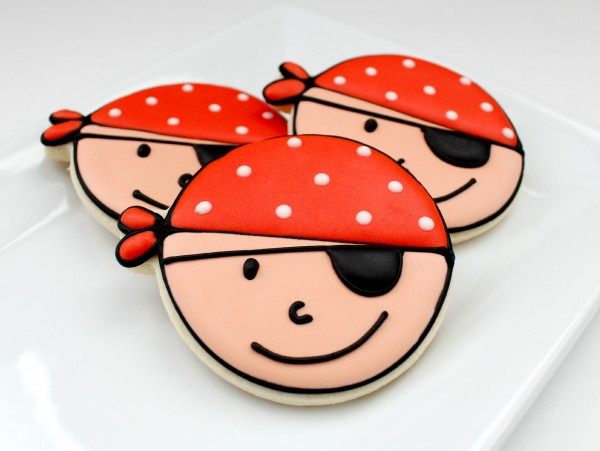
\includegraphics[width=0.5\linewidth]{images/piratecookies} 

}

\end{figure}

Let's say you had a bake sale on your ship where 5 pirates sold both
pies and cookies. You could record the total number of pies and cookies
sold in two vectors:

\begin{Shaded}
\begin{Highlighting}[]
\NormalTok{pies <-}\StringTok{ }\KeywordTok{c}\NormalTok{(}\DecValTok{3}\NormalTok{, }\DecValTok{6}\NormalTok{, }\DecValTok{2}\NormalTok{, }\DecValTok{10}\NormalTok{, }\DecValTok{4}\NormalTok{)}
\NormalTok{cookies <-}\StringTok{ }\KeywordTok{c}\NormalTok{(}\DecValTok{70}\NormalTok{, }\DecValTok{40}\NormalTok{, }\DecValTok{40}\NormalTok{, }\DecValTok{200}\NormalTok{, }\DecValTok{60}\NormalTok{)}
\end{Highlighting}
\end{Shaded}

Now, let's say you want to know how many total items each pirate sold.
You can do this by just adding the two vectors:

\begin{Shaded}
\begin{Highlighting}[]
\NormalTok{total.sold <-}\StringTok{ }\NormalTok{pies }\OperatorTok{+}\StringTok{ }\NormalTok{cookies}
\NormalTok{total.sold}
\NormalTok{## [1]  73  46  42 210  64}
\end{Highlighting}
\end{Shaded}

Crazy.

\section{Summary statistics}\label{summary-statistics}

Ok, now that we can create vectors, let's learn the basic descriptive
statistics functions. We'll start with functions that apply to
continuous data. Continuous data is data that, generally speaking, can
take on an infinite number of values. Height and weight are good
examples of continuous data. Table
\ref{tab:continuousvectorfunctiontable} contains common functions for
continuous, numeric vectors. Each of them takes a numeric vector as an
argument, and returns either a scalar (or in the case of
\texttt{summary()}, a \texttt{table}) as a result.

\begin{longtable}[]{@{}lll@{}}
\caption{\label{tab:continuousvectorfunctiontable} Summary statistic
functions for continuous data.}\tabularnewline
\toprule
\begin{minipage}[b]{0.27\columnwidth}\raggedright\strut
Function\strut
\end{minipage} & \begin{minipage}[b]{0.30\columnwidth}\raggedright\strut
Example\strut
\end{minipage} & \begin{minipage}[b]{0.32\columnwidth}\raggedright\strut
Result\strut
\end{minipage}\tabularnewline
\midrule
\endfirsthead
\toprule
\begin{minipage}[b]{0.27\columnwidth}\raggedright\strut
Function\strut
\end{minipage} & \begin{minipage}[b]{0.30\columnwidth}\raggedright\strut
Example\strut
\end{minipage} & \begin{minipage}[b]{0.32\columnwidth}\raggedright\strut
Result\strut
\end{minipage}\tabularnewline
\midrule
\endhead
\begin{minipage}[t]{0.27\columnwidth}\raggedright\strut
\texttt{sum(x),\ product(x)}\strut
\end{minipage} & \begin{minipage}[t]{0.30\columnwidth}\raggedright\strut
\texttt{sum(1:10)}\strut
\end{minipage} & \begin{minipage}[t]{0.32\columnwidth}\raggedright\strut
55\strut
\end{minipage}\tabularnewline
\begin{minipage}[t]{0.27\columnwidth}\raggedright\strut
\texttt{min(x),\ max(x)}\strut
\end{minipage} & \begin{minipage}[t]{0.30\columnwidth}\raggedright\strut
\texttt{min(1:10)}\strut
\end{minipage} & \begin{minipage}[t]{0.32\columnwidth}\raggedright\strut
1\strut
\end{minipage}\tabularnewline
\begin{minipage}[t]{0.27\columnwidth}\raggedright\strut
\texttt{mean(x),\ median(x)}\strut
\end{minipage} & \begin{minipage}[t]{0.30\columnwidth}\raggedright\strut
\texttt{mean(1:10)}\strut
\end{minipage} & \begin{minipage}[t]{0.32\columnwidth}\raggedright\strut
5.5\strut
\end{minipage}\tabularnewline
\begin{minipage}[t]{0.27\columnwidth}\raggedright\strut
\texttt{sd(x),\ var(x),\ range(x)}\strut
\end{minipage} & \begin{minipage}[t]{0.30\columnwidth}\raggedright\strut
\texttt{sd(1:10)}\strut
\end{minipage} & \begin{minipage}[t]{0.32\columnwidth}\raggedright\strut
3.03\strut
\end{minipage}\tabularnewline
\begin{minipage}[t]{0.27\columnwidth}\raggedright\strut
\texttt{quantile(x,\ probs)}\strut
\end{minipage} & \begin{minipage}[t]{0.30\columnwidth}\raggedright\strut
\texttt{quantile(1:10,\ probs\ =\ .2)}\strut
\end{minipage} & \begin{minipage}[t]{0.32\columnwidth}\raggedright\strut
2.8\strut
\end{minipage}\tabularnewline
\begin{minipage}[t]{0.27\columnwidth}\raggedright\strut
\texttt{summary(x)}\strut
\end{minipage} & \begin{minipage}[t]{0.30\columnwidth}\raggedright\strut
\texttt{summary(1:10)}\strut
\end{minipage} & \begin{minipage}[t]{0.32\columnwidth}\raggedright\strut
\texttt{Min\ =\ 1.00.\ 1st\ Qu.\ =\ 3.25,\ Median\ =\ 5.50,\ Mean\ =\ 5.50,\ 3rd\ Qu.\ =\ 7.75,\ Max\ =\ 10.0}\strut
\end{minipage}\tabularnewline
\bottomrule
\end{longtable}

Let's calculate some descriptive statistics from some pirate related
data. I'll create a vector called \texttt{x} that contains the number of
tattoos from 10 random pirates.

\begin{Shaded}
\begin{Highlighting}[]
\NormalTok{tattoos <-}\StringTok{ }\KeywordTok{c}\NormalTok{(}\DecValTok{4}\NormalTok{, }\DecValTok{50}\NormalTok{, }\DecValTok{2}\NormalTok{, }\DecValTok{39}\NormalTok{, }\DecValTok{4}\NormalTok{, }\DecValTok{20}\NormalTok{, }\DecValTok{4}\NormalTok{, }\DecValTok{8}\NormalTok{, }\DecValTok{10}\NormalTok{, }\DecValTok{100}\NormalTok{)}
\end{Highlighting}
\end{Shaded}

Now, we can calculate several descriptive statistics on this vector by
using the summary statistics functions:

\begin{Shaded}
\begin{Highlighting}[]
\KeywordTok{min}\NormalTok{(tattoos)}
\NormalTok{## [1] 2}
\KeywordTok{mean}\NormalTok{(tattoos)}
\NormalTok{## [1] 24}
\KeywordTok{sd}\NormalTok{(tattoos)}
\NormalTok{## [1] 31}
\end{Highlighting}
\end{Shaded}

\subsection{length()}\label{length}

\begin{figure}

{\centering 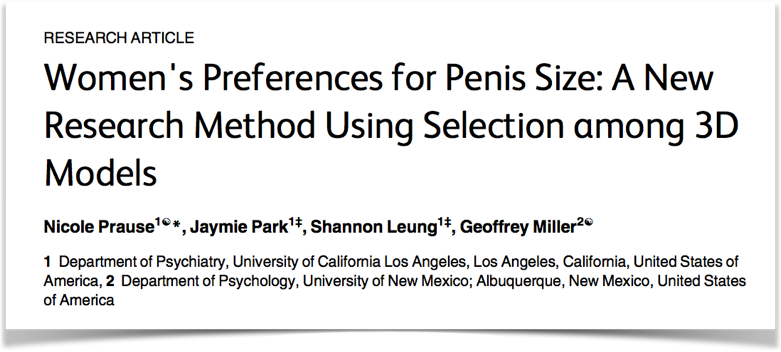
\includegraphics[width=0.5\linewidth]{images/penissize} 

}

\caption{According to this article published in 2015 in Plos One, when it comes to people, length may matter for some. But trust me, for vectors it always does.}\label{fig:unnamed-chunk-121}
\end{figure}

Vectors have one dimension: their length. Later on, when you combine
vectors into more higher dimensional objects, like matrices and
dataframes, you will need to make sure that all the vectors you combine
have the same length. But, when you want to know the length of a vector,
don't stare at your computer screen and count the elements one by one!
(That said, I must admit that I still do this sometimes\ldots{}).
Instead, use \texttt{length()} function. The \texttt{length()} function
takes a vector as an argument, and returns a scalar representing the
number of elements in the vector:

\begin{Shaded}
\begin{Highlighting}[]
\NormalTok{a <-}\StringTok{ }\DecValTok{1}\OperatorTok{:}\DecValTok{10}
\KeywordTok{length}\NormalTok{(a)  }\CommentTok{# How many elements are in a?}
\NormalTok{## [1] 10}

\NormalTok{b <-}\StringTok{ }\KeywordTok{seq}\NormalTok{(}\DataTypeTok{from =} \DecValTok{1}\NormalTok{, }\DataTypeTok{to =} \DecValTok{100}\NormalTok{, }\DataTypeTok{length.out =} \DecValTok{20}\NormalTok{)}
\KeywordTok{length}\NormalTok{(b)  }\CommentTok{# How many elements are in b?}
\NormalTok{## [1] 20}

\KeywordTok{length}\NormalTok{(}\KeywordTok{c}\NormalTok{(}\StringTok{"This"}\NormalTok{, }\StringTok{"character"}\NormalTok{, }\StringTok{"vector"}\NormalTok{, }\StringTok{"has"}\NormalTok{, }\StringTok{"six"}\NormalTok{, }\StringTok{"elements."}\NormalTok{))}
\NormalTok{## [1] 6}
\KeywordTok{length}\NormalTok{(}\StringTok{"This character scalar has just one element."}\NormalTok{)}
\NormalTok{## [1] 1}
\end{Highlighting}
\end{Shaded}

Get used to the \texttt{length()} function people, you'll be using it a
lot!

\subsection{Additional numeric vector
functions}\label{additional-numeric-vector-functions}

Table \ref{tab:morenumericfunctions} contains additional functions that
you will find useful when managing numeric vectors:

\begin{longtable}[]{@{}llll@{}}
\caption{\label{tab:morenumericfunctions} Vector summary functions for
continuous data.}\tabularnewline
\toprule
\begin{minipage}[b]{0.17\columnwidth}\raggedright\strut
Function\strut
\end{minipage} & \begin{minipage}[b]{0.24\columnwidth}\raggedright\strut
Description\strut
\end{minipage} & \begin{minipage}[b]{0.33\columnwidth}\raggedright\strut
Example\strut
\end{minipage} & \begin{minipage}[b]{0.15\columnwidth}\raggedright\strut
Result\strut
\end{minipage}\tabularnewline
\midrule
\endfirsthead
\toprule
\begin{minipage}[b]{0.17\columnwidth}\raggedright\strut
Function\strut
\end{minipage} & \begin{minipage}[b]{0.24\columnwidth}\raggedright\strut
Description\strut
\end{minipage} & \begin{minipage}[b]{0.33\columnwidth}\raggedright\strut
Example\strut
\end{minipage} & \begin{minipage}[b]{0.15\columnwidth}\raggedright\strut
Result\strut
\end{minipage}\tabularnewline
\midrule
\endhead
\begin{minipage}[t]{0.17\columnwidth}\raggedright\strut
\texttt{round(x,\ digits)}\strut
\end{minipage} & \begin{minipage}[t]{0.24\columnwidth}\raggedright\strut
Round elements in x to \texttt{digits} digits\strut
\end{minipage} & \begin{minipage}[t]{0.33\columnwidth}\raggedright\strut
\texttt{round(c(2.231,\ 3.1415),\ digits\ =\ 1)}\strut
\end{minipage} & \begin{minipage}[t]{0.15\columnwidth}\raggedright\strut
2.2, 3.1\strut
\end{minipage}\tabularnewline
\begin{minipage}[t]{0.17\columnwidth}\raggedright\strut
\texttt{ceiling(x),\ floor(x)}\strut
\end{minipage} & \begin{minipage}[t]{0.24\columnwidth}\raggedright\strut
Round elements x to the next highest (or lowest) integer\strut
\end{minipage} & \begin{minipage}[t]{0.33\columnwidth}\raggedright\strut
\texttt{ceiling(c(5.1,\ 7.9))}\strut
\end{minipage} & \begin{minipage}[t]{0.15\columnwidth}\raggedright\strut
6, 8\strut
\end{minipage}\tabularnewline
\begin{minipage}[t]{0.17\columnwidth}\raggedright\strut
\texttt{x\ \%\%\ y}\strut
\end{minipage} & \begin{minipage}[t]{0.24\columnwidth}\raggedright\strut
Modular arithmetic (ie. x mod y)\strut
\end{minipage} & \begin{minipage}[t]{0.33\columnwidth}\raggedright\strut
\texttt{7\ \%\%\ 3}\strut
\end{minipage} & \begin{minipage}[t]{0.15\columnwidth}\raggedright\strut
1\strut
\end{minipage}\tabularnewline
\bottomrule
\end{longtable}

\subsection{Sample statistics from random
samples}\label{sample-statistics-from-random-samples}

Now that you know how to calculate summary statistics, let's take a
closer look at how R draws random samples using the \texttt{rnorm()} and
\texttt{runif()} functions. In the next code chunk, I'll calculate some
summary statistics from a vector of 5 values from a Normal distribution
with a mean of 10 and a standard deviation of 5. I'll then calculate
summary statistics from this sample using \texttt{mean()} and
\texttt{sd()}:

\begin{Shaded}
\begin{Highlighting}[]
\CommentTok{# 5 samples from a Normal dist with mean = 10 and sd = 5}
\NormalTok{x <-}\StringTok{ }\KeywordTok{rnorm}\NormalTok{(}\DataTypeTok{n =} \DecValTok{5}\NormalTok{, }\DataTypeTok{mean =} \DecValTok{10}\NormalTok{, }\DataTypeTok{sd =} \DecValTok{5}\NormalTok{)}

\CommentTok{# What are the mean and standard deviation of the sample?}
\KeywordTok{mean}\NormalTok{(x)}
\NormalTok{## [1] 11}
\KeywordTok{sd}\NormalTok{(x)}
\NormalTok{## [1] 2.5}
\end{Highlighting}
\end{Shaded}

As you can see, the mean and standard deviation of our sample vector are
close to the population values of 10 and 5 -- but they aren't exactly
the same because these are sample data. If we take a much larger sample
(say, 100,000), the sample statistics should get much closer to the
population values:

\begin{Shaded}
\begin{Highlighting}[]
\CommentTok{# 100,000 samples from a Normal dist with mean = 10, sd = 5}
\NormalTok{y <-}\StringTok{ }\KeywordTok{rnorm}\NormalTok{(}\DataTypeTok{n =} \DecValTok{100000}\NormalTok{, }\DataTypeTok{mean =} \DecValTok{10}\NormalTok{, }\DataTypeTok{sd =} \DecValTok{5}\NormalTok{)}

\KeywordTok{mean}\NormalTok{(y)}
\NormalTok{## [1] 10}
\KeywordTok{sd}\NormalTok{(y)}
\NormalTok{## [1] 5}
\end{Highlighting}
\end{Shaded}

Yep, sure enough our new sample y (containing 100,000 values) has a
sample mean and standard deviation much closer (almost identical) to the
population values than our sample x (containing only 5 values). This is
an example of what is called the law of large numbers. Google it.

\section{Counting statistics}\label{counting-statistics}

Next, we'll move on to common counting functions for vectors with
discrete or non-numeric data. Discrete data are those like gender,
occupation, and monkey farts, that only allow for a finite (or at least,
plausibly finite) set of responses. Common functions for discrete
vectors are in Table \ref{tab:discretevectorfunctiontable}. Each of
these vectors takes a vector as an argument -- however, unlike the
previous functions we looked at, the arguments to these functions can be
either numeric or character.

\begin{longtable}[]{@{}llll@{}}
\caption{\label{tab:discretevectorfunctiontable} Counting functions for
discrete data.}\tabularnewline
\toprule
\begin{minipage}[b]{0.13\columnwidth}\raggedright\strut
Function\strut
\end{minipage} & \begin{minipage}[b]{0.23\columnwidth}\raggedright\strut
Description\strut
\end{minipage} & \begin{minipage}[b]{0.29\columnwidth}\raggedright\strut
Example\strut
\end{minipage} & \begin{minipage}[b]{0.23\columnwidth}\raggedright\strut
Result\strut
\end{minipage}\tabularnewline
\midrule
\endfirsthead
\toprule
\begin{minipage}[b]{0.13\columnwidth}\raggedright\strut
Function\strut
\end{minipage} & \begin{minipage}[b]{0.23\columnwidth}\raggedright\strut
Description\strut
\end{minipage} & \begin{minipage}[b]{0.29\columnwidth}\raggedright\strut
Example\strut
\end{minipage} & \begin{minipage}[b]{0.23\columnwidth}\raggedright\strut
Result\strut
\end{minipage}\tabularnewline
\midrule
\endhead
\begin{minipage}[t]{0.13\columnwidth}\raggedright\strut
\texttt{unique(x)}\strut
\end{minipage} & \begin{minipage}[t]{0.23\columnwidth}\raggedright\strut
Returns a vector of all unique values.\strut
\end{minipage} & \begin{minipage}[t]{0.29\columnwidth}\raggedright\strut
\texttt{unique(c(1,\ 1,\ 2,\ 10))}\strut
\end{minipage} & \begin{minipage}[t]{0.23\columnwidth}\raggedright\strut
1, 2, 10\strut
\end{minipage}\tabularnewline
\begin{minipage}[t]{0.13\columnwidth}\raggedright\strut
\texttt{table(x,\ exclude)}\strut
\end{minipage} & \begin{minipage}[t]{0.23\columnwidth}\raggedright\strut
Returns a table showing all the unique values as well as a count of each
occurrence. To include a count of NA values, include the argument
\texttt{exclude\ =\ NULL}\strut
\end{minipage} & \begin{minipage}[t]{0.29\columnwidth}\raggedright\strut
\texttt{table(c("a",\ "a",\ "b",\ "c"))}\strut
\end{minipage} & \begin{minipage}[t]{0.23\columnwidth}\raggedright\strut
\texttt{2-"a",\ 1-"b",\ 1-"c"}\strut
\end{minipage}\tabularnewline
\bottomrule
\end{longtable}

Let's test these functions by starting with two vectors of discrete
data:

\begin{Shaded}
\begin{Highlighting}[]
\NormalTok{vec <-}\StringTok{ }\KeywordTok{c}\NormalTok{(}\DecValTok{1}\NormalTok{, }\DecValTok{1}\NormalTok{, }\DecValTok{1}\NormalTok{, }\DecValTok{5}\NormalTok{, }\DecValTok{1}\NormalTok{, }\DecValTok{1}\NormalTok{, }\DecValTok{10}\NormalTok{, }\DecValTok{10}\NormalTok{, }\DecValTok{10}\NormalTok{)}
\NormalTok{gender <-}\StringTok{ }\KeywordTok{c}\NormalTok{(}\StringTok{"M"}\NormalTok{, }\StringTok{"M"}\NormalTok{, }\StringTok{"F"}\NormalTok{, }\StringTok{"F"}\NormalTok{, }\StringTok{"F"}\NormalTok{, }\StringTok{"M"}\NormalTok{, }\StringTok{"F"}\NormalTok{, }\StringTok{"M"}\NormalTok{, }\StringTok{"F"}\NormalTok{)}
\end{Highlighting}
\end{Shaded}

The function \texttt{unique(x)} will tell you all the unique values in
the vector, but won't tell you anything about how often each value
occurs.

\begin{Shaded}
\begin{Highlighting}[]
\KeywordTok{unique}\NormalTok{(vec)}
\NormalTok{## [1]  1  5 10}
\KeywordTok{unique}\NormalTok{(gender)}
\NormalTok{## [1] "M" "F"}
\end{Highlighting}
\end{Shaded}

The function \texttt{table()} does the same thing as \texttt{unique()},
but goes a step further in telling you how often each of the unique
values occurs:

\begin{Shaded}
\begin{Highlighting}[]
\KeywordTok{table}\NormalTok{(vec)}
\NormalTok{## vec}
\NormalTok{##  1  5 10 }
\NormalTok{##  5  1  3}
\KeywordTok{table}\NormalTok{(gender)}
\NormalTok{## gender}
\NormalTok{## F M }
\NormalTok{## 5 4}
\end{Highlighting}
\end{Shaded}

If you want to get a table of percentages instead of counts, you can
just divide the result of the \texttt{table()} function by the sum of
the result:

\begin{Shaded}
\begin{Highlighting}[]
\KeywordTok{table}\NormalTok{(vec) }\OperatorTok{/}\StringTok{ }\KeywordTok{sum}\NormalTok{(}\KeywordTok{table}\NormalTok{(vec))}
\NormalTok{## vec}
\NormalTok{##    1    5   10 }
\NormalTok{## 0.56 0.11 0.33}
\KeywordTok{table}\NormalTok{(gender) }\OperatorTok{/}\StringTok{ }\KeywordTok{sum}\NormalTok{(}\KeywordTok{table}\NormalTok{(gender))}
\NormalTok{## gender}
\NormalTok{##    F    M }
\NormalTok{## 0.56 0.44}
\end{Highlighting}
\end{Shaded}

\section{Missing (NA) values}\label{missing-na-values}

In R, missing data are coded as NA. In real datasets, NA values turn up
all the time. Unfortunately, most descriptive statistics functions will
freak out if there is a missing (NA) value in the data. For example, the
following code will return NA as a result because there is an NA value
in the data vector:

\begin{Shaded}
\begin{Highlighting}[]
\NormalTok{a <-}\StringTok{ }\KeywordTok{c}\NormalTok{(}\DecValTok{1}\NormalTok{, }\DecValTok{5}\NormalTok{, }\OtherTok{NA}\NormalTok{, }\DecValTok{2}\NormalTok{, }\DecValTok{10}\NormalTok{)}
\KeywordTok{mean}\NormalTok{(a)}
\NormalTok{## [1] NA}
\end{Highlighting}
\end{Shaded}

Thankfully, there's a way we can work around this. To tell a descriptive
statistic function to ignore missing (NA) values, include the argument
\texttt{na.rm\ =\ TRUE} in the function. This argument explicitly tells
the function to ignore NA values. Let's try calculating the mean of the
vector \texttt{a} again, this time with the
additional\texttt{na.rm\ =\ TRUE} argument:

\begin{Shaded}
\begin{Highlighting}[]
\KeywordTok{mean}\NormalTok{(a, }\DataTypeTok{na.rm =} \OtherTok{TRUE}\NormalTok{)}
\NormalTok{## [1] 4.5}
\end{Highlighting}
\end{Shaded}

Now, the function ignored the NA value and returned the mean of the
remaining data. While this may seem trivial now (why did we include an
NA value in the vector if we wanted to ignore it?!), it will be become
very important when we apply the function to real data which, very
often, contains missing values.

\section{Standardization (z-score)}\label{standardization-z-score}

A common task in statistics is to standardize variables -- also known as
calculating z-scores. The purpose of standardizing a vector is to put it
on a common scale which allows you to compare it to other (standardized)
variables. To standardize a vector, you simply subtract the vector by
its mean, and then divide the result by the vector's standard deviation.

If the concept of z-scores is new to you -- don't worry. In the next
worked example, you'll see how it can help you compare two sets of data.
But for now, let's see how easy it is to standardize a vector using
basic arithmetic.

Let's say you have a vector a containing some data. We'll assign the
vector to a new object called \texttt{a} then calculate the mean and
standard deviation with the \texttt{mean()} and \texttt{sd()} functions:

\begin{Shaded}
\begin{Highlighting}[]
\NormalTok{a <-}\StringTok{ }\KeywordTok{c}\NormalTok{(}\DecValTok{5}\NormalTok{, }\DecValTok{3}\NormalTok{, }\DecValTok{7}\NormalTok{, }\DecValTok{5}\NormalTok{, }\DecValTok{5}\NormalTok{, }\DecValTok{3}\NormalTok{, }\DecValTok{4}\NormalTok{)}
\KeywordTok{mean}\NormalTok{(a)}
\NormalTok{## [1] 4.6}
\KeywordTok{sd}\NormalTok{(a)}
\NormalTok{## [1] 1.4}
\end{Highlighting}
\end{Shaded}

Ok. Now we'll create a new vector called \texttt{a.z} which is a
standardized version of a. To do this, we'll simply subtract the mean of
the vector, then divide by the standard deviation.

\begin{Shaded}
\begin{Highlighting}[]
\NormalTok{a.z <-}\StringTok{ }\NormalTok{(a }\OperatorTok{-}\StringTok{ }\KeywordTok{mean}\NormalTok{(a)) }\OperatorTok{/}\StringTok{ }\KeywordTok{sd}\NormalTok{(a)}
\end{Highlighting}
\end{Shaded}

Now let's look at the standardized values:

\begin{Shaded}
\begin{Highlighting}[]
\NormalTok{a.z}
\NormalTok{## [1]  0.31 -1.12  1.74  0.31  0.31 -1.12 -0.41}
\end{Highlighting}
\end{Shaded}

The mean of \texttt{a.z} should now be 0, and the standard deviation of
\texttt{a.z} should now be 1. Let's make sure:

\begin{Shaded}
\begin{Highlighting}[]
\KeywordTok{mean}\NormalTok{(a.z)}
\NormalTok{## [1] 2e-16}
\KeywordTok{sd}\NormalTok{(a.z)}
\NormalTok{## [1] 1}
\end{Highlighting}
\end{Shaded}

Sweet. Oh, don't worry that the mean of \texttt{a.z} doesn't look like
exactly zero. Using non-scientific notation, the result is
0.000000000000000198. For all intents and purposes, that's 0. The reason
the result is not exactly 0 is due to computer science theoretical
reasons that I cannot explain (because I don't understand them).

\subsection{Ex: Evaluating a
competition}\label{ex-evaluating-a-competition}

Your gluten-intolerant first mate just perished in a tragic soy sauce
incident and it's time to promote another member of your crew to the
newly vacated position. Of course, only two qualities really matter for
a pirate: rope-climbing, and grogg drinking. Therefore, to see which of
your crew deserves the promotion, you decide to hold a climbing and
drinking competition. In the climbing competition, you measure how many
feet of rope a pirate can climb in an hour. In the drinking competition,
you measure how many mugs of grogg they can drink in a minute. Five
pirates volunteer for the competition -- here are their results:

\begin{table}

\caption{\label{tab:unnamed-chunk-136}Scores from a pirate competition}
\centering
\begin{tabular}[t]{l|r|r}
\hline
pirate & grogg & climbing\\
\hline
Heidi & 12 & 100\\
\hline
Andrew & 8 & 520\\
\hline
Becki & 1 & 430\\
\hline
Madisen & 6 & 200\\
\hline
David & 2 & 700\\
\hline
\end{tabular}
\end{table}

We can represent the main results with two vectors \texttt{grogg} and
\texttt{climbing}:

\begin{Shaded}
\begin{Highlighting}[]
\NormalTok{grogg <-}\StringTok{ }\KeywordTok{c}\NormalTok{(}\DecValTok{12}\NormalTok{, }\DecValTok{8}\NormalTok{, }\DecValTok{1}\NormalTok{, }\DecValTok{6}\NormalTok{, }\DecValTok{2}\NormalTok{)}
\NormalTok{climbing <-}\StringTok{ }\KeywordTok{c}\NormalTok{(}\DecValTok{100}\NormalTok{, }\DecValTok{520}\NormalTok{, }\DecValTok{430}\NormalTok{, }\DecValTok{200}\NormalTok{, }\DecValTok{700}\NormalTok{)}
\end{Highlighting}
\end{Shaded}

Now you've got the data, but there's a problem: the scales of the
numbers are very different. While the grogg numbers range from 1 to 12,
the climbing numbers have a much larger range from 100 to 700. This
makes it difficult to compare the two sets of numbers directly.

To solve this problem, we'll use standardization. Let's create new
standardized vectors called \texttt{grogg.z} and \texttt{climbing.z}

\begin{Shaded}
\begin{Highlighting}[]
\NormalTok{grogg.z <-}\StringTok{ }\NormalTok{(grogg }\OperatorTok{-}\StringTok{ }\KeywordTok{mean}\NormalTok{(grogg)) }\OperatorTok{/}\StringTok{ }\KeywordTok{sd}\NormalTok{(grogg)}
\NormalTok{climbing.z <-}\StringTok{ }\NormalTok{(climbing }\OperatorTok{-}\StringTok{ }\KeywordTok{mean}\NormalTok{(climbing)) }\OperatorTok{/}\StringTok{ }\KeywordTok{sd}\NormalTok{(climbing)}
\end{Highlighting}
\end{Shaded}

Now let's look at the final results

\begin{Shaded}
\begin{Highlighting}[]
\NormalTok{grogg.z}
\NormalTok{## [1]  1.379  0.489 -1.068  0.044 -0.845}
\NormalTok{climbing.z}
\NormalTok{## [1] -1.20  0.54  0.17 -0.78  1.28}
\end{Highlighting}
\end{Shaded}

It looks like there were two outstanding performances in particular. In
the grogg drinking competition, the first pirate (Heidi) had a z-score
of 1.4. We can interpret this by saying that Heidi drank 1.4 more
standard deviations of mugs of grogg than the average pirate. In the
climbing competition, the fifth pirate (David) had a z-score of 1.3.
Here, we would conclude that David climbed 1.3 standard deviations more
than the average pirate.

But which pirate was the best on average across both events? To answer
this, let's create a combined z-score for each pirate which calculates
the average z-scores for each pirate across the two events. We'll do
this by adding two performances and dividing by two. This will tell us,
how good, on average, each pirate did relative to her fellow pirates.

\begin{Shaded}
\begin{Highlighting}[]
\NormalTok{average.z <-}\StringTok{ }\NormalTok{(grogg.z }\OperatorTok{+}\StringTok{ }\NormalTok{(climbing.z)) }\OperatorTok{/}\StringTok{ }\DecValTok{2}
\end{Highlighting}
\end{Shaded}

Let's look at the result:

\begin{Shaded}
\begin{Highlighting}[]
\KeywordTok{round}\NormalTok{(average.z, }\DecValTok{1}\NormalTok{)}
\NormalTok{## [1]  0.1  0.5 -0.5 -0.4  0.2}
\end{Highlighting}
\end{Shaded}

The highest average z-score belongs to the second pirate (Andrew) who
had an average z-score value of 0.5. The first and last pirates, who did
well in one event, seemed to have done poorly in the other event.

Moral of the story: promote the pirate who can drink \emph{and} climb.

\section{Test your R Might!}\label{test-your-r-might-2}

\begin{enumerate}
\def\labelenumi{\arabic{enumi}.}
\item
  Create a vector that shows the square root of the integers from 1 to
  10.
\item
  Renata thinks that she finds more treasure when she's had a mug of
  grogg than when she doesn't. To test this, she recorded how much
  treasure she found over 7 days without drinking any grogg (ie.,
  sober), and then did the same over 7 days while drinking grogg (ie.,
  drunk). Here are her results:
\end{enumerate}

\begin{table}

\caption{\label{tab:unnamed-chunk-143}Renata's treasure haul when she was sober and when she was drunk}
\centering
\begin{tabular}[t]{l|r|r}
\hline
day & sober & drunk\\
\hline
Monday & 2 & 0\\
\hline
Tuesday & 0 & 0\\
\hline
Wednesday & 3 & 1\\
\hline
Thursday & 1 & 0\\
\hline
Friday & 0 & 1\\
\hline
Saturday & 3 & 2\\
\hline
Sunday & 5 & 2\\
\hline
\end{tabular}
\end{table}

How much treasure did Renata find on average when she was sober? What
about when she was drunk?

\begin{enumerate}
\def\labelenumi{\arabic{enumi}.}
\setcounter{enumi}{2}
\item
  Using Renata's data again, create a new vector called
  \texttt{difference} that shows how much more treasure Renata found
  when she was drunk and when she was not. What was the mean, median,
  and standard deviation of the difference?
\item
  There's an old parable that goes something like this. A man does some
  work for a king and needs to be paid. Because the man loves rice (who
  doesn't?!), the man offers the king two different ways that he can be
  paid. \emph{You can either pay me 100 kilograms of rice, or, you can
  pay me as follows: get a chessboard and put one grain of rice in the
  top left square. Then put 2 grains of rice on the next square,
  followed by 4 grains on the next, 8 grains on the next\ldots{}and so
  on, where the amount of rice doubles on each square, until you get to
  the last square. When you are finished, give me all the grains of rice
  that would (in theory), fit on the chessboard.} The king, sensing that
  the man was an idiot for making such a stupid offer, immediately
  accepts the second option. He summons a chessboard, and begins
  counting out grains of rice one by one\ldots{} Assuming that there are
  64 squares on a chessboard, calculate how many grains of rice the main
  will receive. If one grain of rice weights 1/6400 kilograms, how many
  kilograms of rice did he get? \emph{Hint: If you have trouble coming
  up with the answer, imagine how many grains are on the first, second,
  third and fourth squares, then try to create the vector that shows the
  number of grains on each square. Once you come up with that vector,
  you can easily calculate the final answer with the \texttt{sum()}
  function.}
\end{enumerate}

\chapter{Indexing Vectors with {[} {]}}\label{vectorindexing}

\begin{tabular}{l|l|r|r|r}
\hline
boat.names & boat.colors & boat.ages & boat.prices & boat.costs\\
\hline
a & black & 143 & 53 & 52\\
\hline
b & green & 53 & 87 & 80\\
\hline
c & pink & 356 & 54 & 20\\
\hline
d & blue & 23 & 66 & 100\\
\hline
e & blue & 647 & 264 & 189\\
\hline
f & green & 24 & 32 & 12\\
\hline
g & green & 532 & 532 & 520\\
\hline
h & yellow & 43 & 58 & 68\\
\hline
i & black & 66 & 99 & 80\\
\hline
j & black & 86 & 132 & 100\\
\hline
\end{tabular}

\begin{Shaded}
\begin{Highlighting}[]
\CommentTok{# Boat sale. Creating the data vectors}
\NormalTok{boat.names <-}\StringTok{ }\KeywordTok{c}\NormalTok{(}\StringTok{"a"}\NormalTok{, }\StringTok{"b"}\NormalTok{, }\StringTok{"c"}\NormalTok{, }\StringTok{"d"}\NormalTok{, }\StringTok{"e"}\NormalTok{, }\StringTok{"f"}\NormalTok{, }\StringTok{"g"}\NormalTok{, }\StringTok{"h"}\NormalTok{, }\StringTok{"i"}\NormalTok{, }\StringTok{"j"}\NormalTok{)}
\NormalTok{boat.colors <-}\StringTok{ }\KeywordTok{c}\NormalTok{(}\StringTok{"black"}\NormalTok{, }\StringTok{"green"}\NormalTok{, }\StringTok{"pink"}\NormalTok{, }\StringTok{"blue"}\NormalTok{, }\StringTok{"blue"}\NormalTok{, }
                \StringTok{"green"}\NormalTok{, }\StringTok{"green"}\NormalTok{, }\StringTok{"yellow"}\NormalTok{, }\StringTok{"black"}\NormalTok{, }\StringTok{"black"}\NormalTok{)}
\NormalTok{boat.ages <-}\StringTok{ }\KeywordTok{c}\NormalTok{(}\DecValTok{143}\NormalTok{, }\DecValTok{53}\NormalTok{, }\DecValTok{356}\NormalTok{, }\DecValTok{23}\NormalTok{, }\DecValTok{647}\NormalTok{, }\DecValTok{24}\NormalTok{, }\DecValTok{532}\NormalTok{, }\DecValTok{43}\NormalTok{, }\DecValTok{66}\NormalTok{, }\DecValTok{86}\NormalTok{)}
\NormalTok{boat.prices <-}\StringTok{ }\KeywordTok{c}\NormalTok{(}\DecValTok{53}\NormalTok{, }\DecValTok{87}\NormalTok{, }\DecValTok{54}\NormalTok{, }\DecValTok{66}\NormalTok{, }\DecValTok{264}\NormalTok{, }\DecValTok{32}\NormalTok{, }\DecValTok{532}\NormalTok{, }\DecValTok{58}\NormalTok{, }\DecValTok{99}\NormalTok{, }\DecValTok{132}\NormalTok{)}
\NormalTok{boat.costs <-}\StringTok{ }\KeywordTok{c}\NormalTok{(}\DecValTok{52}\NormalTok{, }\DecValTok{80}\NormalTok{, }\DecValTok{20}\NormalTok{, }\DecValTok{100}\NormalTok{, }\DecValTok{189}\NormalTok{, }\DecValTok{12}\NormalTok{, }\DecValTok{520}\NormalTok{, }\DecValTok{68}\NormalTok{, }\DecValTok{80}\NormalTok{, }\DecValTok{100}\NormalTok{)}

\CommentTok{# What was the price of the first boat?}
\NormalTok{boat.prices[}\DecValTok{1}\NormalTok{]}
\NormalTok{## [1] 53}

\CommentTok{# What were the ages of the first 5 boats?}
\NormalTok{boat.ages[}\DecValTok{1}\OperatorTok{:}\DecValTok{5}\NormalTok{]}
\NormalTok{## [1] 143  53 356  23 647}

\CommentTok{# What were the names of the black boats?}
\NormalTok{boat.names[boat.colors }\OperatorTok{==}\StringTok{ "black"}\NormalTok{]}
\NormalTok{## [1] "a" "i" "j"}

\CommentTok{# What were the prices of either green or yellow boats?}
\NormalTok{boat.prices[boat.colors }\OperatorTok{==}\StringTok{ "green"} \OperatorTok{|}\StringTok{ }\NormalTok{boat.colors }\OperatorTok{==}\StringTok{ "yellow"}\NormalTok{]}
\NormalTok{## [1]  87  32 532  58}

\CommentTok{# Change the price of boat "s" to 100}
\NormalTok{boat.prices[boat.names }\OperatorTok{==}\StringTok{ "s"}\NormalTok{] <-}\StringTok{ }\DecValTok{100}

\CommentTok{# What was the median price of black boats less than 100 years old?}
\KeywordTok{median}\NormalTok{(boat.prices[boat.colors }\OperatorTok{==}\StringTok{ "black"} \OperatorTok{&}\StringTok{ }\NormalTok{boat.ages }\OperatorTok{<}\StringTok{ }\DecValTok{100}\NormalTok{])}
\NormalTok{## [1] 116}

\CommentTok{# How many pink boats were there?}
\KeywordTok{sum}\NormalTok{(boat.colors }\OperatorTok{==}\StringTok{ "pink"}\NormalTok{)}
\NormalTok{## [1] 1}

\CommentTok{# What percent of boats were older than 100 years old?}
\KeywordTok{mean}\NormalTok{(boat.ages }\OperatorTok{<}\StringTok{ }\DecValTok{100}\NormalTok{)}
\NormalTok{## [1] 0.6}
\end{Highlighting}
\end{Shaded}

By now you should be a whiz at applying functions like \texttt{mean()}
and \texttt{table()} to vectors. However, in many analyses, you won't
want to calculate statistics of an entire vector. Instead, you will want
to access specific \emph{subsets} of values of a vector based on some
criteria. For example, you may want to access values in a specific
location in the vector (i.e.; the first 10 elements) or based on some
criteria within that vector (i.e.; all values greater than 0), or based
on criterion from values in a \emph{different} vector (e.g.; All values
of age where sex is Female). To access specific values of a vector in R,
we use \emph{indexing} using brackets \texttt{{[}{]}}. In general,
whatever you put inside the brackets, tells R which values of the vector
object you want. There are two main ways that you can use indexing to
access subsets of data in a vector: numerical and logical indexing.

\section{Numerical Indexing}\label{numerical-indexing}

With numerical indexing, you enter a vector of integers corresponding to
the values in the vector you want to access in the form
\texttt{a{[}index{]}}, where \texttt{a} is the vector, and
\texttt{index} is a vector of index values. For example, let's use
numerical indexing to get values from our boat vectors.

\begin{Shaded}
\begin{Highlighting}[]
\CommentTok{# What is the first boat name?}
\NormalTok{boat.names[}\DecValTok{1}\NormalTok{]}
\NormalTok{## [1] "a"}

\CommentTok{# What are the first five boat colors?}
\NormalTok{boat.colors[}\DecValTok{1}\OperatorTok{:}\DecValTok{5}\NormalTok{]}
\NormalTok{## [1] "black" "green" "pink"  "blue"  "blue"}

\CommentTok{# What is every second boat age?}
\NormalTok{boat.ages[}\KeywordTok{seq}\NormalTok{(}\DecValTok{1}\NormalTok{, }\DecValTok{5}\NormalTok{, }\DataTypeTok{by =} \DecValTok{2}\NormalTok{)]}
\NormalTok{## [1] 143 356 647}
\end{Highlighting}
\end{Shaded}

You can use any indexing vector as long as it contains integers. You can
even access the same elements multiple times:

\begin{Shaded}
\begin{Highlighting}[]
\CommentTok{# What is the first boat age (3 times)}
\NormalTok{boat.ages[}\KeywordTok{c}\NormalTok{(}\DecValTok{1}\NormalTok{, }\DecValTok{1}\NormalTok{, }\DecValTok{1}\NormalTok{)]}
\NormalTok{## [1] 143 143 143}
\end{Highlighting}
\end{Shaded}

If it makes your code clearer, you can define an indexing object before
doing your actual indexing. For example, let's define an object called
\texttt{my.index} and use this object to index our data vector:

\begin{Shaded}
\begin{Highlighting}[]
\NormalTok{my.index <-}\StringTok{ }\DecValTok{3}\OperatorTok{:}\DecValTok{5}
\NormalTok{boat.names[my.index]}
\NormalTok{## [1] "c" "d" "e"}
\end{Highlighting}
\end{Shaded}

\section{Logical Indexing}\label{logical-indexing}

\begin{figure}

{\centering 
\includegraphics[width=0.5\linewidth]{images/logic} 

}

\caption{Logical indexing. Good for R aliens and R pirates.}\label{fig:unnamed-chunk-151}
\end{figure}

The second way to index vectors is with \emph{logical vectors}. A
logical vector is a vector that \emph{only} contains TRUE and FALSE
values. In R, true values are designated with TRUE, and false values
with FALSE. When you index a vector with a logical vector, R will return
values of the vector for which the indexing vector is TRUE. If that was
confusing, think about it this way: a logical vector, combined with the
brackets \texttt{{[}\ {]}}, acts as a \emph{filter} for the vector it is
indexing. It only lets values of the vector pass through for which the
logical vector is TRUE.

\begin{figure}

{\centering 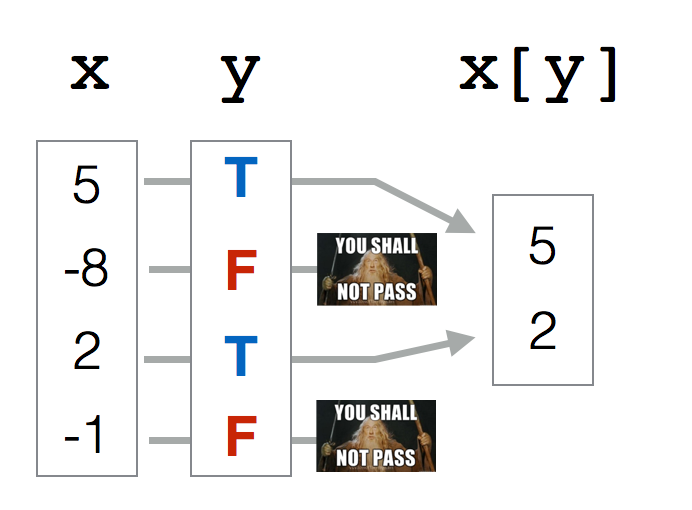
\includegraphics[width=0.5\linewidth]{images/indexgandolf} 

}

\caption{FALSE values in a logical vector are like lots of mini-Gandolfs. In this example, I am indexing a vector x with a logical vector y (y for example could be x > 0, so all positive values of x are TRUE and all negative values are FALSE). The result is a vector of length 2, which are the values of x for which the logical vector y was true. Gandolf stopped all the values of x for which y was FALSE.}\label{fig:unnamed-chunk-152}
\end{figure}

You could create logical vectors directly using \texttt{c()}. For
example, I could access every other value of the following vector as
follows:

\begin{Shaded}
\begin{Highlighting}[]
\NormalTok{a <-}\StringTok{ }\KeywordTok{c}\NormalTok{(}\DecValTok{1}\NormalTok{, }\DecValTok{2}\NormalTok{, }\DecValTok{3}\NormalTok{, }\DecValTok{4}\NormalTok{, }\DecValTok{5}\NormalTok{)}
\NormalTok{a[}\KeywordTok{c}\NormalTok{(}\OtherTok{TRUE}\NormalTok{, }\OtherTok{FALSE}\NormalTok{, }\OtherTok{TRUE}\NormalTok{, }\OtherTok{FALSE}\NormalTok{, }\OtherTok{TRUE}\NormalTok{)]}
\NormalTok{## [1] 1 3 5}
\end{Highlighting}
\end{Shaded}

As you can see, R returns all values of the vector \texttt{a} for which
the logical vector is TRUE.

\begin{figure}
\centering
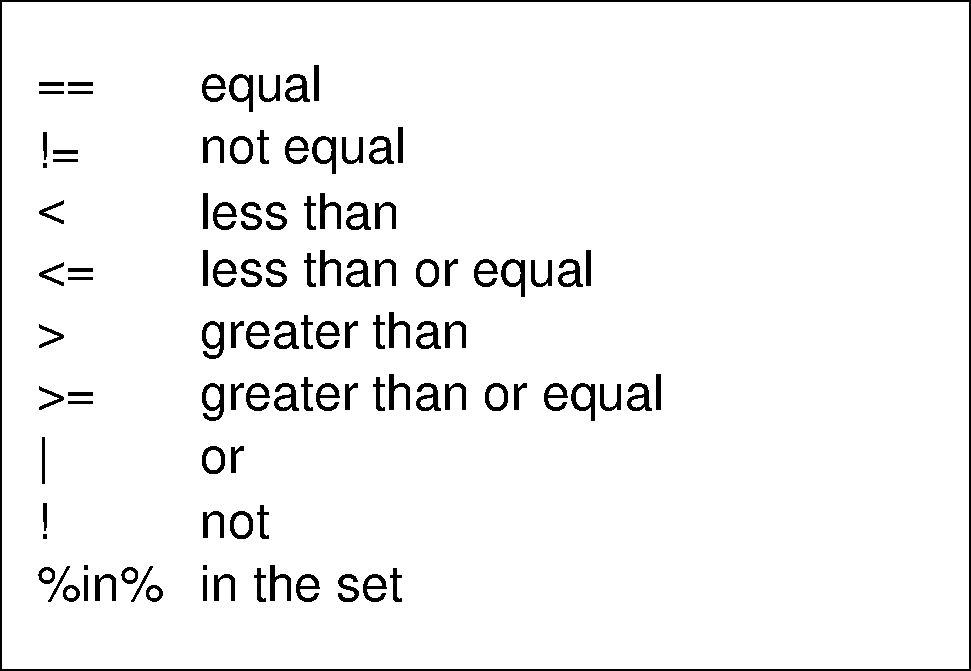
\includegraphics{YaRrr_files/figure-latex/comparison-1.pdf}
\caption{\label{fig:comparison}Logical comparison operators in R}
\end{figure}

However, creating logical vectors using \texttt{c()} is tedious.
Instead, it's better to create logical vectors from \emph{existing
vectors} using comparison operators like \textless{} (less than), ==
(equals to), and != (not equal to). A complete list of the most common
comparison operators is in Figure \ref{fig:comparison}. For example,
let's create some logical vectors from our \texttt{boat.ages} vector:

\begin{Shaded}
\begin{Highlighting}[]
\CommentTok{# Which ages are > 100?}
\NormalTok{boat.ages }\OperatorTok{>}\StringTok{ }\DecValTok{100}
\NormalTok{##  [1]  TRUE FALSE  TRUE FALSE  TRUE FALSE  TRUE FALSE FALSE FALSE}

\CommentTok{# Which ages are equal to 23?}
\NormalTok{boat.ages }\OperatorTok{==}\StringTok{ }\DecValTok{23}
\NormalTok{##  [1] FALSE FALSE FALSE  TRUE FALSE FALSE FALSE FALSE FALSE FALSE}

\CommentTok{# Which boat names are equal to c?}
\NormalTok{boat.names }\OperatorTok{==}\StringTok{ "c"}
\NormalTok{##  [1] FALSE FALSE  TRUE FALSE FALSE FALSE FALSE FALSE FALSE FALSE}
\end{Highlighting}
\end{Shaded}

You can also create logical vectors by comparing a vector to another
vector of the same length. When you do this, R will compare values in
the same position (e.g.; the first values will be compared, then the
second values, etc.). For example, we can compare the \texttt{boat.cost}
and \texttt{boat.price} vectors to see which boats sold for a higher
price than their cost:

\begin{Shaded}
\begin{Highlighting}[]
\CommentTok{# Which boats had a higher price than cost?}
\NormalTok{boat.prices }\OperatorTok{>}\StringTok{ }\NormalTok{boat.costs}
\NormalTok{##  [1]  TRUE  TRUE  TRUE FALSE  TRUE  TRUE  TRUE FALSE  TRUE  TRUE}

\CommentTok{# Which boats had a lower price than cost?}
\NormalTok{boat.prices }\OperatorTok{<}\StringTok{ }\NormalTok{boat.costs}
\NormalTok{##  [1] FALSE FALSE FALSE  TRUE FALSE FALSE FALSE  TRUE FALSE FALSE}
\end{Highlighting}
\end{Shaded}

Once you've created a logical vector using a comparison operator, you
can use it to index any vector with the same length. Here, I'll use
logical vectors to get the prices of boats whose ages were greater than
100:

\begin{Shaded}
\begin{Highlighting}[]
\CommentTok{# What were the prices of boats older than 100?}
\NormalTok{boat.prices[boat.ages }\OperatorTok{>}\StringTok{ }\DecValTok{100}\NormalTok{]}
\NormalTok{## [1]  53  54 264 532}
\end{Highlighting}
\end{Shaded}

Here's how logical indexing works step-by-step:

\begin{Shaded}
\begin{Highlighting}[]
\CommentTok{# Which boats are older than 100 years?}
\NormalTok{boat.ages }\OperatorTok{>}\StringTok{ }\DecValTok{100}
\NormalTok{##  [1]  TRUE FALSE  TRUE FALSE  TRUE FALSE  TRUE FALSE FALSE FALSE}

\CommentTok{# Writing the logical index by hand (you'd never do this!)}
\CommentTok{#  Show me all of the boat prices where the logical vector is TRUE:}
\NormalTok{boat.prices[}\KeywordTok{c}\NormalTok{(}\OtherTok{TRUE}\NormalTok{, }\OtherTok{FALSE}\NormalTok{, }\OtherTok{TRUE}\NormalTok{, }\OtherTok{FALSE}\NormalTok{, }\OtherTok{TRUE}\NormalTok{, }\OtherTok{FALSE}\NormalTok{, }\OtherTok{TRUE}\NormalTok{, }\OtherTok{FALSE}\NormalTok{, }\OtherTok{FALSE}\NormalTok{, }\OtherTok{FALSE}\NormalTok{)]}
\NormalTok{## [1]  53  54 264 532}

\CommentTok{# Doing it all in one step! You get the same answer:}
\NormalTok{boat.prices[boat.ages }\OperatorTok{>}\StringTok{ }\DecValTok{100}\NormalTok{]}
\NormalTok{## [1]  53  54 264 532}
\end{Highlighting}
\end{Shaded}

\subsection{\texorpdfstring{\texttt{\&} (and), \texttt{\textbar{}} (or),
\texttt{\%in\%}}{\& (and), \textbar{} (or), \%in\%}}\label{and-or-in}

In addition to using single comparison operators, you can combine
multiple logical vectors using the OR (which looks like
\texttt{\textbar{}} and AND \texttt{\&} commands. The OR
\texttt{\textbar{}} operation will return TRUE if any of the logical
vectors is TRUE, while the AND \texttt{\&} operation will only return
TRUE if all of the values in the logical vectors is TRUE. This is
especially powerful when you want to create a logical vector based on
criteria from multiple vectors.

For example, let's create a logical vector indicating which boats had a
price greater than 200 OR less than 100, and then use that vector to see
what the names of these boats were:

\begin{Shaded}
\begin{Highlighting}[]
\CommentTok{# Which boats had prices greater than 200 OR less than 100?}
\NormalTok{boat.prices }\OperatorTok{>}\StringTok{ }\DecValTok{200} \OperatorTok{|}\StringTok{ }\NormalTok{boat.prices }\OperatorTok{<}\StringTok{ }\DecValTok{100}
\NormalTok{##  [1]  TRUE  TRUE  TRUE  TRUE  TRUE  TRUE  TRUE  TRUE  TRUE FALSE}

\CommentTok{# What were the NAMES of these boats}
\NormalTok{boat.names[boat.prices }\OperatorTok{>}\StringTok{ }\DecValTok{200} \OperatorTok{|}\StringTok{ }\NormalTok{boat.prices }\OperatorTok{<}\StringTok{ }\DecValTok{100}\NormalTok{]}
\NormalTok{## [1] "a" "b" "c" "d" "e" "f" "g" "h" "i"}
\end{Highlighting}
\end{Shaded}

You can combine as many logical vectors as you want (as long as they all
have the same length!):

\begin{Shaded}
\begin{Highlighting}[]
\CommentTok{# Boat names of boats with a color of black OR with a price > 100}
\NormalTok{boat.names[boat.colors }\OperatorTok{==}\StringTok{ "black"} \OperatorTok{|}\StringTok{ }\NormalTok{boat.prices }\OperatorTok{>}\StringTok{ }\DecValTok{100}\NormalTok{]}
\NormalTok{## [1] "a" "e" "g" "i" "j"}

\CommentTok{# Names of blue boats with a price greater than 200}
\NormalTok{boat.names[boat.colors }\OperatorTok{==}\StringTok{ "blue"} \OperatorTok{&}\StringTok{ }\NormalTok{boat.prices }\OperatorTok{>}\StringTok{ }\DecValTok{200}\NormalTok{]}
\NormalTok{## [1] "e"}
\end{Highlighting}
\end{Shaded}

You can combine as many logical vectors as you want to create
increasingly complex selection criteria. For example, the following
logical vector returns TRUE for cases where the boat colors are black OR
brown, AND where the price was less than 100:

\begin{Shaded}
\begin{Highlighting}[]
\CommentTok{# Which boats were eithe black or brown, AND had a price less than 100?}
\NormalTok{(boat.colors }\OperatorTok{==}\StringTok{ "black"} \OperatorTok{|}\StringTok{ }\NormalTok{boat.colors }\OperatorTok{==}\StringTok{ "brown"}\NormalTok{) }\OperatorTok{&}\StringTok{ }\NormalTok{boat.prices }\OperatorTok{<}\StringTok{ }\DecValTok{100}
\NormalTok{##  [1]  TRUE FALSE FALSE FALSE FALSE FALSE FALSE FALSE  TRUE FALSE}

\CommentTok{# What were the names of these boats?}
\NormalTok{boat.names[(boat.colors }\OperatorTok{==}\StringTok{ "black"} \OperatorTok{|}\StringTok{ }\NormalTok{boat.colors }\OperatorTok{==}\StringTok{ "brown"}\NormalTok{) }\OperatorTok{&}\StringTok{ }\NormalTok{boat.prices }\OperatorTok{<}\StringTok{ }\DecValTok{100}\NormalTok{]}
\NormalTok{## [1] "a" "i"}
\end{Highlighting}
\end{Shaded}

When using multiple criteria, make sure to use parentheses when
appropriate. If I didn't use parentheses above, I would get a different
answer.

The \texttt{\%in\%} operation helps you to easily create multiple OR
arguments.Imagine you have a vector of categorical data that can take on
many different values. For example, you could have a vector x indicating
people's favorite letters.

\begin{Shaded}
\begin{Highlighting}[]
\NormalTok{x <-}\StringTok{ }\KeywordTok{c}\NormalTok{(}\StringTok{"a"}\NormalTok{, }\StringTok{"t"}\NormalTok{, }\StringTok{"a"}\NormalTok{, }\StringTok{"b"}\NormalTok{, }\StringTok{"z"}\NormalTok{)}
\end{Highlighting}
\end{Shaded}

Now, let's say you want to create a logical vector indicating which
values are either a or b or c or d. You could create this logical vector
with multiple \textbar{} (OR) commands:

\begin{Shaded}
\begin{Highlighting}[]
\NormalTok{x }\OperatorTok{==}\StringTok{ "a"} \OperatorTok{|}\StringTok{ }\NormalTok{x }\OperatorTok{==}\StringTok{ "b"} \OperatorTok{|}\StringTok{ }\NormalTok{x }\OperatorTok{==}\StringTok{ "c"} \OperatorTok{|}\StringTok{ }\NormalTok{x }\OperatorTok{==}\StringTok{ "d"}
\NormalTok{## [1]  TRUE FALSE  TRUE  TRUE FALSE}
\end{Highlighting}
\end{Shaded}

However, this takes a long time to write. Thankfully, the
\texttt{\%in\%} operation allows you to combine multiple OR comparisons
much faster. To use the \texttt{\%in\%} function, just put it in between
the original vector, and a new vector of possible values. The
\texttt{\%in\%} function goes through every value in the vector x, and
returns TRUE if it finds it in the vector of possible values --
otherwise it returns FALSE.

\begin{Shaded}
\begin{Highlighting}[]
\NormalTok{x }\OperatorTok\StringTok{ }\KeywordTok{c}\NormalTok{(}\StringTok{"a"}\NormalTok{, }\StringTok{"b"}\NormalTok{, }\StringTok{"c"}\NormalTok{, }\StringTok{"d"}\NormalTok{)}
\NormalTok{## [1]  TRUE FALSE  TRUE  TRUE FALSE}
\end{Highlighting}
\end{Shaded}

As you can see, the result is identical to our previous result.

\subsection{Counts and percentages from logical
vectors}\label{counts-and-percentages-from-logical-vectors}

Many (if not all) R functions will interpret TRUE values as 1 and FALSE
values as 0. This allows us to easily answer questions like ``How many
values in a data vector are greater than 0?'' or ``What percentage of
values are equal to 5?'' by applying the \texttt{sum()} or
\texttt{mean()} function to a logical vector.

We'll start with a vector x of length 10, containing 3 positive numbers
and 5 negative numbers.

\begin{Shaded}
\begin{Highlighting}[]
\NormalTok{x <-}\StringTok{ }\KeywordTok{c}\NormalTok{(}\DecValTok{1}\NormalTok{, }\DecValTok{2}\NormalTok{, }\DecValTok{3}\NormalTok{, }\OperatorTok{-}\DecValTok{5}\NormalTok{, }\OperatorTok{-}\DecValTok{5}\NormalTok{, }\OperatorTok{-}\DecValTok{5}\NormalTok{, }\OperatorTok{-}\DecValTok{5}\NormalTok{, }\OperatorTok{-}\DecValTok{5}\NormalTok{)}
\end{Highlighting}
\end{Shaded}

We can create a logical vector to see which values are greater than 0:

\begin{Shaded}
\begin{Highlighting}[]
\NormalTok{x }\OperatorTok{>}\StringTok{ }\DecValTok{0}
\NormalTok{## [1]  TRUE  TRUE  TRUE FALSE FALSE FALSE FALSE FALSE}
\end{Highlighting}
\end{Shaded}

Now, we'll use \texttt{sum()} and \texttt{mean()} on that logical vector
to see how many of the values in x are positive, and what percent are
positive. We should find that there are 5 TRUE values, and that 50\% of
the values (5 / 10) are TRUE.

\begin{Shaded}
\begin{Highlighting}[]
\KeywordTok{sum}\NormalTok{(x }\OperatorTok{>}\StringTok{ }\DecValTok{0}\NormalTok{)}
\NormalTok{## [1] 3}
\KeywordTok{mean}\NormalTok{(x }\OperatorTok{>}\StringTok{ }\DecValTok{0}\NormalTok{)}
\NormalTok{## [1] 0.38}
\end{Highlighting}
\end{Shaded}

This is a \emph{really} powerful tool. Pretty much \emph{any} time you
want to answer a question like ``How many of X are Y'' or ``What percent
of X are Y'', you use \texttt{sum()} or \texttt{mean()} function with a
logical vector as an argument.

\subsection{Additional Logical
functions}\label{additional-logical-functions}

R has lots of special functions that take vectors as arguments, and
return logical vectors based on multiple criteria. For example, you can
use the \texttt{is.na()} function to test which values of a vector are
missing. Table \ref{tab:logicalfunctions} contains some that I
frequently use:

\begin{longtable}[]{@{}llll@{}}
\caption{\label{tab:logicalfunctions} Functions to create and use logical
vectors.}\tabularnewline
\toprule
\begin{minipage}[b]{0.20\columnwidth}\raggedright\strut
Function\strut
\end{minipage} & \begin{minipage}[b]{0.23\columnwidth}\raggedright\strut
Description\strut
\end{minipage} & \begin{minipage}[b]{0.31\columnwidth}\raggedright\strut
Example\strut
\end{minipage} & \begin{minipage}[b]{0.06\columnwidth}\raggedright\strut
Result\strut
\end{minipage}\tabularnewline
\midrule
\endfirsthead
\toprule
\begin{minipage}[b]{0.20\columnwidth}\raggedright\strut
Function\strut
\end{minipage} & \begin{minipage}[b]{0.23\columnwidth}\raggedright\strut
Description\strut
\end{minipage} & \begin{minipage}[b]{0.31\columnwidth}\raggedright\strut
Example\strut
\end{minipage} & \begin{minipage}[b]{0.06\columnwidth}\raggedright\strut
Result\strut
\end{minipage}\tabularnewline
\midrule
\endhead
\begin{minipage}[t]{0.20\columnwidth}\raggedright\strut
\texttt{is.na(x)}\strut
\end{minipage} & \begin{minipage}[t]{0.23\columnwidth}\raggedright\strut
Which values in x are NA?\strut
\end{minipage} & \begin{minipage}[t]{0.31\columnwidth}\raggedright\strut
\texttt{is.na(c(2,\ NA,\ 5))}\strut
\end{minipage} & \begin{minipage}[t]{0.06\columnwidth}\raggedright\strut
FALSE, TRUE, FALSE\strut
\end{minipage}\tabularnewline
\begin{minipage}[t]{0.20\columnwidth}\raggedright\strut
\texttt{is.finite(x)}\strut
\end{minipage} & \begin{minipage}[t]{0.23\columnwidth}\raggedright\strut
Which values in x are numbers?\strut
\end{minipage} & \begin{minipage}[t]{0.31\columnwidth}\raggedright\strut
\texttt{is.finite(c(NA,\ 89,\ 0))}\strut
\end{minipage} & \begin{minipage}[t]{0.06\columnwidth}\raggedright\strut
FALSE, TRUE, TRUE\strut
\end{minipage}\tabularnewline
\begin{minipage}[t]{0.20\columnwidth}\raggedright\strut
\texttt{duplicated(x)}\strut
\end{minipage} & \begin{minipage}[t]{0.23\columnwidth}\raggedright\strut
Which values in x are duplicated?\strut
\end{minipage} & \begin{minipage}[t]{0.31\columnwidth}\raggedright\strut
\texttt{duplicated(c(1,\ 4,\ 1,\ 2))}\strut
\end{minipage} & \begin{minipage}[t]{0.06\columnwidth}\raggedright\strut
FALSE, FALSE, TRUE, FALSE\strut
\end{minipage}\tabularnewline
\begin{minipage}[t]{0.20\columnwidth}\raggedright\strut
\texttt{which(x)}\strut
\end{minipage} & \begin{minipage}[t]{0.23\columnwidth}\raggedright\strut
Which values in x are TRUE?\strut
\end{minipage} & \begin{minipage}[t]{0.31\columnwidth}\raggedright\strut
\texttt{which(c(TRUE,\ FALSE,\ TRUE))}\strut
\end{minipage} & \begin{minipage}[t]{0.06\columnwidth}\raggedright\strut
1, 3\strut
\end{minipage}\tabularnewline
\bottomrule
\end{longtable}

Logical vectors aren't just good for indexing, you can also use them to
figure out which values in a vector satisfy some criteria. To do this,
use the function \texttt{which()}. If you apply the function
\texttt{which()} to a logical vector, R will tell you which values of
the index are TRUE. For example:

\begin{Shaded}
\begin{Highlighting}[]
\CommentTok{# A vector of sex information}
\NormalTok{sex <-}\StringTok{ }\KeywordTok{c}\NormalTok{(}\StringTok{"m"}\NormalTok{, }\StringTok{"m"}\NormalTok{, }\StringTok{"f"}\NormalTok{, }\StringTok{"m"}\NormalTok{, }\StringTok{"f"}\NormalTok{, }\StringTok{"f"}\NormalTok{)}

\CommentTok{# Which values of sex are m?}
\KeywordTok{which}\NormalTok{(sex }\OperatorTok{==}\StringTok{ "m"}\NormalTok{)}
\NormalTok{## [1] 1 2 4}

\CommentTok{# Which values of sex are f?}
\KeywordTok{which}\NormalTok{(sex }\OperatorTok{==}\StringTok{ "f"}\NormalTok{)}
\NormalTok{## [1] 3 5 6}
\end{Highlighting}
\end{Shaded}

\section{Changing values of a vector}\label{changing-values-of-a-vector}

Now that you know how to index a vector, you can easily change specific
values in a vector using the assignment (\texttt{\textless{}-})
operation. To do this, just assign a vector of new values to the indexed
values of the original vector:

Let's create a vector \texttt{a} which contains 10 1s:

\begin{Shaded}
\begin{Highlighting}[]
\NormalTok{a <-}\StringTok{ }\KeywordTok{rep}\NormalTok{(}\DecValTok{1}\NormalTok{, }\DecValTok{10}\NormalTok{)}
\end{Highlighting}
\end{Shaded}

Now, let's change the first 5 values in the vector to 9s by indexing the
first five values, and assigning the value of 9:

\begin{Shaded}
\begin{Highlighting}[]
\NormalTok{a[}\DecValTok{1}\OperatorTok{:}\DecValTok{5}\NormalTok{] <-}\StringTok{ }\DecValTok{9}
\NormalTok{a}
\NormalTok{##  [1] 9 9 9 9 9 1 1 1 1 1}
\end{Highlighting}
\end{Shaded}

Now let's change the last 5 values to 0s. We'll index the values 6
through 10, and assign a value of 0.

\begin{Shaded}
\begin{Highlighting}[]
\NormalTok{a[}\DecValTok{6}\OperatorTok{:}\DecValTok{10}\NormalTok{] <-}\StringTok{ }\DecValTok{0}
\NormalTok{a}
\NormalTok{##  [1] 9 9 9 9 9 0 0 0 0 0}
\end{Highlighting}
\end{Shaded}

Of course, you can also change values of a vector using a logical
indexing vector. For example, let's say you have a vector of numbers
that should be from 1 to 10. If values are outside of this range, you
want to set them to either the minimum (1) or maximum (10) value:

\begin{Shaded}
\begin{Highlighting}[]
\CommentTok{# x is a vector of numbers that should be from 1 to 10}
\NormalTok{x <-}\StringTok{ }\KeywordTok{c}\NormalTok{(}\DecValTok{5}\NormalTok{, }\OperatorTok{-}\DecValTok{5}\NormalTok{, }\DecValTok{7}\NormalTok{, }\DecValTok{4}\NormalTok{, }\DecValTok{11}\NormalTok{, }\DecValTok{5}\NormalTok{, }\OperatorTok{-}\DecValTok{2}\NormalTok{)}

\CommentTok{# Assign values less than 1 to 1}
\NormalTok{x[x }\OperatorTok{<}\StringTok{ }\DecValTok{1}\NormalTok{] <-}\StringTok{ }\DecValTok{1}

\CommentTok{# Assign values greater than 10 to 10}
\NormalTok{x[x }\OperatorTok{>}\StringTok{ }\DecValTok{10}\NormalTok{] <-}\StringTok{ }\DecValTok{10}

\CommentTok{# Print the result!}
\NormalTok{x}
\NormalTok{## [1]  5  1  7  4 10  5  1}
\end{Highlighting}
\end{Shaded}

As you can see, our new values of x are now never less than 1 or greater
than 10!

\textbf{A note on indexing\ldots{}}

Technically, when you assign new values to a vector, you should always
assign a vector of the same length as the number of values that you are
updating. For example, given a vector a with 10 1s:

\begin{Shaded}
\begin{Highlighting}[]
\NormalTok{a <-}\StringTok{ }\KeywordTok{rep}\NormalTok{(}\DecValTok{1}\NormalTok{, }\DecValTok{10}\NormalTok{)}
\end{Highlighting}
\end{Shaded}

To update the first 5 values with 5 9s, we should assign a new vector of
5 9s

\begin{Shaded}
\begin{Highlighting}[]
\NormalTok{a[}\DecValTok{1}\OperatorTok{:}\DecValTok{5}\NormalTok{] <-}\StringTok{ }\KeywordTok{c}\NormalTok{(}\DecValTok{9}\NormalTok{, }\DecValTok{9}\NormalTok{, }\DecValTok{9}\NormalTok{, }\DecValTok{9}\NormalTok{, }\DecValTok{9}\NormalTok{)}
\NormalTok{a}
\NormalTok{##  [1] 9 9 9 9 9 1 1 1 1 1}
\end{Highlighting}
\end{Shaded}

However, if we repeat this code but just assign a single 9, R will
repeat the value as many times as necessary to fill the indexed value of
the vector. That's why the following code still works:

\begin{Shaded}
\begin{Highlighting}[]
\NormalTok{a[}\DecValTok{1}\OperatorTok{:}\DecValTok{5}\NormalTok{] <-}\StringTok{ }\DecValTok{9}
\NormalTok{a}
\NormalTok{##  [1] 9 9 9 9 9 1 1 1 1 1}
\end{Highlighting}
\end{Shaded}

In other languages this code wouldn't work because we're trying to
replace 5 values with just 1. However, this is a case where R bends the
rules a bit.

\subsection{Ex: Fixing invalid responses to a Happiness
survey}\label{ex-fixing-invalid-responses-to-a-happiness-survey}

\begin{figure}

{\centering \includegraphics[width=0.5\linewidth]{images/happiness} 

}

\end{figure}

Assigning and indexing is a particularly helpful tool when, for example,
you want to remove invalid values in a vector before performing an
analysis. For example, let's say you asked 10 people how happy they were
on a scale of 1 to 5 and received the following responses:

\begin{Shaded}
\begin{Highlighting}[]
\NormalTok{happy <-}\StringTok{ }\KeywordTok{c}\NormalTok{(}\DecValTok{1}\NormalTok{, }\DecValTok{4}\NormalTok{, }\DecValTok{2}\NormalTok{, }\DecValTok{999}\NormalTok{, }\DecValTok{2}\NormalTok{, }\DecValTok{3}\NormalTok{, }\OperatorTok{-}\DecValTok{2}\NormalTok{, }\DecValTok{3}\NormalTok{, }\DecValTok{2}\NormalTok{, }\DecValTok{999}\NormalTok{)}
\end{Highlighting}
\end{Shaded}

As you can see, we have some invalid values (999 and -2) in this vector.
To remove them, we'll use logical indexing to change the invalid values
(999 and -2) to NA. We'll create a logical vector indicating which
values of \texttt{happy} are \emph{invalid} using the \texttt{\%in\%}
operation. Because we want to see which values are \emph{invalid}, we'll
add the \texttt{==\ FALSE} condition (If we don't, the index will tell
us which values \emph{are} valid).

\begin{Shaded}
\begin{Highlighting}[]
\CommentTok{# Which values of happy are NOT in the set 1:5?}
\NormalTok{invalid <-}\StringTok{ }\NormalTok{(happy }\OperatorTok\StringTok{ }\DecValTok{1}\OperatorTok{:}\DecValTok{5}\NormalTok{) }\OperatorTok{==}\StringTok{ }\OtherTok{FALSE}
\NormalTok{invalid}
\NormalTok{##  [1] FALSE FALSE FALSE  TRUE FALSE FALSE  TRUE FALSE FALSE  TRUE}
\end{Highlighting}
\end{Shaded}

Now that we have a logical index \texttt{invalid} telling us which
values are invalid (that is, not in the set 1 through 5), we'll index
\texttt{happy} with \texttt{invalid}, and assign the invalid values as
NA:

\begin{Shaded}
\begin{Highlighting}[]
\CommentTok{# Convert any invalid values in happy to NA}
\NormalTok{happy[invalid] <-}\StringTok{ }\OtherTok{NA}
\NormalTok{happy}
\NormalTok{##  [1]  1  4  2 NA  2  3 NA  3  2 NA}
\end{Highlighting}
\end{Shaded}

We can also recode all the invalid values of \texttt{happy} in one line
as follows:

\begin{Shaded}
\begin{Highlighting}[]
\CommentTok{# Convert all values of happy that are NOT integers from 1 to 5 to NA}
\NormalTok{happy[(happy }\OperatorTok\StringTok{ }\DecValTok{1}\OperatorTok{:}\DecValTok{5}\NormalTok{) }\OperatorTok{==}\StringTok{ }\OtherTok{FALSE}\NormalTok{] <-}\StringTok{ }\OtherTok{NA}
\end{Highlighting}
\end{Shaded}

As you can see, \texttt{happy} now has NAs for previously invalid
values. Now we can take a \texttt{mean()} of the vector and see the mean
of the valid responses.

\begin{Shaded}
\begin{Highlighting}[]
\CommentTok{# Include na.rm = TRUE to ignore NA values}
\KeywordTok{mean}\NormalTok{(happy, }\DataTypeTok{na.rm =} \OtherTok{TRUE}\NormalTok{)}
\NormalTok{## [1] 2.4}
\end{Highlighting}
\end{Shaded}

\section{Test your R Might!: Movie
data}\label{test-your-r-might-movie-data}

\begin{figure}

{\centering \includegraphics[width=1\linewidth]{images/moviecollage} 

}

\end{figure}

Table \ref{tab:moviedata} contains data about 10 of my favorite movies.

\begin{table}

\caption{\label{tab:moviedata}Some of my favorite movies}
\centering
\begin{tabular}[t]{l|r|r|l|r|l}
\hline
movie & year & boxoffice & genre & time & rating\\
\hline
Whatever Works & 2009 & 35.0 & Comedy & 92 & PG-13\\
\hline
It Follows & 2015 & 15.0 & Horror & 97 & R\\
\hline
Love and Mercy & 2015 & 15.0 & Drama & 120 & R\\
\hline
The Goonies & 1985 & 62.0 & Adventure & 90 & PG\\
\hline
Jiro Dreams of Sushi & 2012 & 3.0 & Documentary & 81 & G\\
\hline
There Will be Blood & 2007 & 10.0 & Drama & 158 & R\\
\hline
Moon & 2009 & 321.0 & Science Fiction & 97 & R\\
\hline
Spice World & 1988 & 79.0 & Comedy & -84 & PG-13\\
\hline
Serenity & 2005 & 39.0 & Science Fiction & 119 & PG-13\\
\hline
Finding Vivian Maier & 2014 & 1.5 & Documentary & 84 & Unrated\\
\hline
\end{tabular}
\end{table}

\begin{enumerate}
\def\labelenumi{\arabic{enumi}.}
\setcounter{enumi}{-1}
\item
  Create new data vectors for each column.
\item
  What is the name of the 10th movie in the list?
\item
  What are the genres of the first 4 movies?
\item
  Some joker put Spice World in the movie names -- it should be ``The
  Naked Gun'' Please correct the name.
\item
  What were the names of the movies made before 1990?
\item
  How many movies were Dramas? What percent of the 10 movies were
  Dramas?
\item
  One of the values in the \texttt{time} vector is invalid. Convert any
  invalid values in this vector to NA. Then, calculate the mean movie
  time
\item
  What were the names of the Comedy movies? What were their boxoffice
  totals? (Two separate questions)
\item
  What were the names of the movies that made less than \$50 Million
  dollars AND were Comedies?
\item
  What was the median boxoffice revenue of movies rated either G or PG?
\item
  What percent of the movies were rated R OR were comedies?
\end{enumerate}

\chapter{Matrices and Dataframes}\label{matricesdataframes}

\begin{figure}

{\centering \includegraphics[width=0.5\linewidth]{images/matrix} 

}

\caption{Did you actually think I could talk about matrices without a Matrix reference?!}\label{fig:unnamed-chunk-183}
\end{figure}

\begin{Shaded}
\begin{Highlighting}[]
\CommentTok{# -----------------------------}
\CommentTok{# Basic dataframe operations}
\CommentTok{# -----------------------------}

\CommentTok{# Create a dataframe of boat sale data called bsale}
\NormalTok{bsale <-}\StringTok{ }\KeywordTok{data.frame}\NormalTok{(}\DataTypeTok{name =} \KeywordTok{c}\NormalTok{(}\StringTok{"a"}\NormalTok{, }\StringTok{"b"}\NormalTok{, }\StringTok{"c"}\NormalTok{, }\StringTok{"d"}\NormalTok{, }\StringTok{"e"}\NormalTok{, }\StringTok{"f"}\NormalTok{, }\StringTok{"g"}\NormalTok{, }\StringTok{"h"}\NormalTok{, }\StringTok{"i"}\NormalTok{, }\StringTok{"j"}\NormalTok{),}
                    \DataTypeTok{color =} \KeywordTok{c}\NormalTok{(}\StringTok{"black"}\NormalTok{, }\StringTok{"green"}\NormalTok{, }\StringTok{"pink"}\NormalTok{, }\StringTok{"blue"}\NormalTok{, }\StringTok{"blue"}\NormalTok{, }
                              \StringTok{"green"}\NormalTok{, }\StringTok{"green"}\NormalTok{, }\StringTok{"yellow"}\NormalTok{, }\StringTok{"black"}\NormalTok{, }\StringTok{"black"}\NormalTok{),}
                    \DataTypeTok{age =} \KeywordTok{c}\NormalTok{(}\DecValTok{143}\NormalTok{, }\DecValTok{53}\NormalTok{, }\DecValTok{356}\NormalTok{, }\DecValTok{23}\NormalTok{, }\DecValTok{647}\NormalTok{, }\DecValTok{24}\NormalTok{, }\DecValTok{532}\NormalTok{, }\DecValTok{43}\NormalTok{, }\DecValTok{66}\NormalTok{, }\DecValTok{86}\NormalTok{),}
                    \DataTypeTok{price =} \KeywordTok{c}\NormalTok{(}\DecValTok{53}\NormalTok{, }\DecValTok{87}\NormalTok{, }\DecValTok{54}\NormalTok{, }\DecValTok{66}\NormalTok{, }\DecValTok{264}\NormalTok{, }\DecValTok{32}\NormalTok{, }\DecValTok{532}\NormalTok{, }\DecValTok{58}\NormalTok{, }\DecValTok{99}\NormalTok{, }\DecValTok{132}\NormalTok{),}
                    \DataTypeTok{cost =} \KeywordTok{c}\NormalTok{(}\DecValTok{52}\NormalTok{, }\DecValTok{80}\NormalTok{, }\DecValTok{20}\NormalTok{, }\DecValTok{100}\NormalTok{, }\DecValTok{189}\NormalTok{, }\DecValTok{12}\NormalTok{, }\DecValTok{520}\NormalTok{, }\DecValTok{68}\NormalTok{, }\DecValTok{80}\NormalTok{, }\DecValTok{100}\NormalTok{),}
                    \DataTypeTok{stringsAsFactors =} \OtherTok{FALSE}\NormalTok{)   }\CommentTok{# Don't convert strings to factors!}

\CommentTok{# Explore the bsale dataset:}
\KeywordTok{head}\NormalTok{(bsale)     }\CommentTok{# Show me the first few rows}
\KeywordTok{str}\NormalTok{(bsale)      }\CommentTok{# Show me the structure of the data}
\KeywordTok{View}\NormalTok{(bsale)     }\CommentTok{# Open the data in a new window}
\KeywordTok{names}\NormalTok{(bsale)    }\CommentTok{# What are the names of the columns?}
\KeywordTok{nrow}\NormalTok{(bsale)     }\CommentTok{# How many rows are there in the data?}

\CommentTok{# Calculating statistics from column vectors}
\KeywordTok{mean}\NormalTok{(bsale}\OperatorTok{$}\NormalTok{age)       }\CommentTok{# What was the mean age?}
\KeywordTok{table}\NormalTok{(bsale}\OperatorTok{$}\NormalTok{color)    }\CommentTok{# How many boats were there of each color?}
\KeywordTok{max}\NormalTok{(bsale}\OperatorTok{$}\NormalTok{price)      }\CommentTok{# What was the maximum price?}

\CommentTok{# Adding new columns}
\NormalTok{bsale}\OperatorTok{$}\NormalTok{id <-}\StringTok{ }\DecValTok{1}\OperatorTok{:}\KeywordTok{nrow}\NormalTok{(bsale)}
\NormalTok{bsale}\OperatorTok{$}\NormalTok{age.decades <-}\StringTok{ }\NormalTok{bsale}\OperatorTok{$}\NormalTok{age }\OperatorTok{/}\StringTok{ }\DecValTok{10}
\NormalTok{bsale}\OperatorTok{$}\NormalTok{profit <-}\StringTok{ }\NormalTok{bsale}\OperatorTok{$}\NormalTok{price }\OperatorTok{-}\StringTok{ }\NormalTok{bsale}\OperatorTok{$}\NormalTok{cost}

\CommentTok{# What was the mean price of green boats?}
\KeywordTok{with}\NormalTok{(bsale, }\KeywordTok{mean}\NormalTok{(price[color }\OperatorTok{==}\StringTok{ "green"}\NormalTok{]))}

\CommentTok{# What were the names of boats older than 100 years?}
\KeywordTok{with}\NormalTok{(bsale, name[age }\OperatorTok{>}\StringTok{ }\DecValTok{100}\NormalTok{])}

\CommentTok{# What percent of black boats had a positive profit?}
\KeywordTok{with}\NormalTok{(}\KeywordTok{subset}\NormalTok{(bsale, color }\OperatorTok{==}\StringTok{ "black"}\NormalTok{), }\KeywordTok{mean}\NormalTok{(profit }\OperatorTok{>}\StringTok{ }\DecValTok{0}\NormalTok{))}

\CommentTok{# Save only the price and cost columns in a new dataframe}
\NormalTok{bsale.}\DecValTok{2}\NormalTok{ <-}\StringTok{ }\NormalTok{bsale[}\KeywordTok{c}\NormalTok{(}\StringTok{"price"}\NormalTok{, }\StringTok{"cost"}\NormalTok{)]}

\CommentTok{# Change the names of the columns to "p" and "c"}
\KeywordTok{names}\NormalTok{(bsale.}\DecValTok{2}\NormalTok{) <-}\StringTok{ }\KeywordTok{c}\NormalTok{(}\StringTok{"p"}\NormalTok{, }\StringTok{"c"}\NormalTok{)}

\CommentTok{# Create a dataframe called old.black.bsale containing only data from black boats older than 50 years}
\NormalTok{old.black.bsale <-}\StringTok{ }\KeywordTok{subset}\NormalTok{(bsale, color }\OperatorTok{==}\StringTok{ "black"} \OperatorTok{&}\StringTok{ }\NormalTok{age }\OperatorTok{>}\StringTok{ }\DecValTok{50}\NormalTok{)}
\end{Highlighting}
\end{Shaded}

\section{What are matrices and
dataframes?}\label{what-are-matrices-and-dataframes}

By now, you should be comfortable with scalar and vector objects.
However, you may have noticed that neither object types are appropriate
for storing lots of data -- such as the results of a survey or
experiment. Thankfully, R has two object types that represent large data
structures much better: \textbf{matrices} and \textbf{dataframes}.

Matrices and dataframes are very similar to spreadsheets in Excel or
data files in SPSS. Every matrix or dataframe contains rows (call that
number m) and columns (n). Thus, wile a vector has 1 dimension (its
length), matrices and dataframes both have 2-dimensions -- representing
their width and height. You can think of a matrix or dataframe as a
combination of \texttt{n} vectors, where each vector has a length of
\texttt{m}.

\begin{figure}
\centering
\includegraphics{YaRrr_files/figure-latex/unnamed-chunk-185-1.pdf}
\caption{\label{fig:unnamed-chunk-185}scalar, Vector, MATRIX}
\end{figure}

While matrices and dataframes look very similar, they aren't exactly the
same. While a matrix can contain \emph{either} character \emph{or}
numeric columns, a dataframe can contain \emph{both} numeric and
character columns. Because dataframes are more flexible, most real-world
datasets, such as surveys containing both numeric (e.g.; age, response
times) and character (e.g.; sex, favorite movie) data, will be stored as
dataframes in R.

\textbf{WTF} -- If dataframes are more flexible than matrices, why do we
use matrices at all? The answer is that, because they are simpler,
matrices take up less computational space than dataframes. Additionally,
some functions require matrices as inputs to ensure that they work
correctly.

In the next section, we'll cover the most common functions for creating
matrix and dataframe objects. We'll then move on to functions that take
matrices and dataframes as inputs.

\section{Creating matrices and
dataframes}\label{creating-matrices-and-dataframes}

There are a number of ways to create your own matrix and dataframe
objects in R. The most common functions are presented in Table
\ref{tab:matrixfunctions}. Because matrices and dataframes are just
combinations of vectors, each function takes one or more vectors as
inputs, and returns a matrix or a dataframe.

\begin{longtable}[]{@{}lll@{}}
\caption{\label{tab:matrixfunctions} Functions to create matrices and
dataframes.}\tabularnewline
\toprule
\begin{minipage}[b]{0.19\columnwidth}\raggedright\strut
Function\strut
\end{minipage} & \begin{minipage}[b]{0.27\columnwidth}\raggedright\strut
Description\strut
\end{minipage} & \begin{minipage}[b]{0.41\columnwidth}\raggedright\strut
Example\strut
\end{minipage}\tabularnewline
\midrule
\endfirsthead
\toprule
\begin{minipage}[b]{0.19\columnwidth}\raggedright\strut
Function\strut
\end{minipage} & \begin{minipage}[b]{0.27\columnwidth}\raggedright\strut
Description\strut
\end{minipage} & \begin{minipage}[b]{0.41\columnwidth}\raggedright\strut
Example\strut
\end{minipage}\tabularnewline
\midrule
\endhead
\begin{minipage}[t]{0.19\columnwidth}\raggedright\strut
\texttt{cbind(a,\ b,\ c)}\strut
\end{minipage} & \begin{minipage}[t]{0.27\columnwidth}\raggedright\strut
Combine vectors as columns in a matrix\strut
\end{minipage} & \begin{minipage}[t]{0.41\columnwidth}\raggedright\strut
\texttt{cbind(1:5,\ 6:10,\ 11:15)}\strut
\end{minipage}\tabularnewline
\begin{minipage}[t]{0.19\columnwidth}\raggedright\strut
\texttt{rbind(a,\ b,\ c)}\strut
\end{minipage} & \begin{minipage}[t]{0.27\columnwidth}\raggedright\strut
Combine vectors as rows in a matrix\strut
\end{minipage} & \begin{minipage}[t]{0.41\columnwidth}\raggedright\strut
\texttt{rbind(1:5,\ 6:10,\ 11:15)}\strut
\end{minipage}\tabularnewline
\begin{minipage}[t]{0.19\columnwidth}\raggedright\strut
\texttt{matrix(x,\ nrow,\ ncol,\ byrow)}\strut
\end{minipage} & \begin{minipage}[t]{0.27\columnwidth}\raggedright\strut
Create a matrix from a vector \texttt{x}\strut
\end{minipage} & \begin{minipage}[t]{0.41\columnwidth}\raggedright\strut
\texttt{matrix(x\ =\ 1:12,\ nrow\ =\ 3,\ ncol\ =\ 4)}\strut
\end{minipage}\tabularnewline
\begin{minipage}[t]{0.19\columnwidth}\raggedright\strut
\texttt{data.frame()}\strut
\end{minipage} & \begin{minipage}[t]{0.27\columnwidth}\raggedright\strut
Create a dataframe from named columns\strut
\end{minipage} & \begin{minipage}[t]{0.41\columnwidth}\raggedright\strut
\texttt{data.frame("age"\ =\ c(19,\ 21),}
\texttt{sex\ =\ c("m",\ "f"))}\strut
\end{minipage}\tabularnewline
\bottomrule
\end{longtable}

\subsection{\texorpdfstring{\texttt{cbind()},
\texttt{rbind()}}{cbind(), rbind()}}\label{cbind-rbind}

\texttt{cbind()} and \texttt{rbind()} both create matrices by combining
several vectors of the same length. \texttt{cbind()} combines vectors as
columns, while \texttt{rbind()} combines them as rows.

Let's use these functions to create a matrix with the numbers 1 through
30. First, we'll create three vectors of length 5, then we'll combine
them into one matrix. As you will see, the \texttt{cbind()} function
will combine the vectors as columns in the final matrix, while the
\texttt{rbind()} function will combine them as rows.

\begin{Shaded}
\begin{Highlighting}[]
\NormalTok{x <-}\StringTok{ }\DecValTok{1}\OperatorTok{:}\DecValTok{5}
\NormalTok{y <-}\StringTok{ }\DecValTok{6}\OperatorTok{:}\DecValTok{10}
\NormalTok{z <-}\StringTok{ }\DecValTok{11}\OperatorTok{:}\DecValTok{15}

\CommentTok{# Create a matrix where x, y and z are columns}
\KeywordTok{cbind}\NormalTok{(x, y, z)}
\NormalTok{##      x  y  z}
\NormalTok{## [1,] 1  6 11}
\NormalTok{## [2,] 2  7 12}
\NormalTok{## [3,] 3  8 13}
\NormalTok{## [4,] 4  9 14}
\NormalTok{## [5,] 5 10 15}

\CommentTok{# Create a matrix where x, y and z are rows}
\KeywordTok{rbind}\NormalTok{(x, y, z)}
\NormalTok{##   [,1] [,2] [,3] [,4] [,5]}
\NormalTok{## x    1    2    3    4    5}
\NormalTok{## y    6    7    8    9   10}
\NormalTok{## z   11   12   13   14   15}
\end{Highlighting}
\end{Shaded}

\subsection{\texorpdfstring{\texttt{matrix()}}{matrix()}}\label{matrix}

\textbf{Remember}: Matrices can either contain numbers \emph{or}
character vectors, not both!. If you try to create a matrix with both
numbers and characters, it will turn all the numbers into characters:

\begin{Shaded}
\begin{Highlighting}[]
\CommentTok{# Creating a matrix with numeric and character columns will make everything a character:}

\KeywordTok{cbind}\NormalTok{(}\KeywordTok{c}\NormalTok{(}\DecValTok{1}\NormalTok{, }\DecValTok{2}\NormalTok{, }\DecValTok{3}\NormalTok{, }\DecValTok{4}\NormalTok{, }\DecValTok{5}\NormalTok{),}
      \KeywordTok{c}\NormalTok{(}\StringTok{"a"}\NormalTok{, }\StringTok{"b"}\NormalTok{, }\StringTok{"c"}\NormalTok{, }\StringTok{"d"}\NormalTok{, }\StringTok{"e"}\NormalTok{))}
\NormalTok{##      [,1] [,2]}
\NormalTok{## [1,] "1"  "a" }
\NormalTok{## [2,] "2"  "b" }
\NormalTok{## [3,] "3"  "c" }
\NormalTok{## [4,] "4"  "d" }
\NormalTok{## [5,] "5"  "e"}
\end{Highlighting}
\end{Shaded}

The \texttt{matrix()} function creates a matrix form a single vector of
data. The function has 4 main inputs: \texttt{data} -- a vector of data,
\texttt{nrow} -- the number of rows you want in the matrix, and
\texttt{ncol} -- the number of columns you want in the matrix, and
\texttt{byrow} -- a logical value indicating whether you want to fill
the matrix by rows. Check out the help menu for the matrix function
(`?matrix) to see some additional inputs.

Let's use the \texttt{matrix()} function to re-create a matrix
containing the values from 1 to 10.

\begin{Shaded}
\begin{Highlighting}[]
\CommentTok{# Create a matrix of the integers 1:10,}
\CommentTok{#  with 5 rows and 2 columns}

\KeywordTok{matrix}\NormalTok{(}\DataTypeTok{data =} \DecValTok{1}\OperatorTok{:}\DecValTok{10}\NormalTok{,}
       \DataTypeTok{nrow =} \DecValTok{5}\NormalTok{,}
       \DataTypeTok{ncol =} \DecValTok{2}\NormalTok{)}
\NormalTok{##      [,1] [,2]}
\NormalTok{## [1,]    1    6}
\NormalTok{## [2,]    2    7}
\NormalTok{## [3,]    3    8}
\NormalTok{## [4,]    4    9}
\NormalTok{## [5,]    5   10}

\CommentTok{# Now with 2 rows and 5 columns}
\KeywordTok{matrix}\NormalTok{(}\DataTypeTok{data =} \DecValTok{1}\OperatorTok{:}\DecValTok{10}\NormalTok{,}
       \DataTypeTok{nrow =} \DecValTok{2}\NormalTok{,}
       \DataTypeTok{ncol =} \DecValTok{5}\NormalTok{)}
\NormalTok{##      [,1] [,2] [,3] [,4] [,5]}
\NormalTok{## [1,]    1    3    5    7    9}
\NormalTok{## [2,]    2    4    6    8   10}

\CommentTok{# Now with 2 rows and 5 columns, but fill by row instead of columns}
\KeywordTok{matrix}\NormalTok{(}\DataTypeTok{data =} \DecValTok{1}\OperatorTok{:}\DecValTok{10}\NormalTok{,}
       \DataTypeTok{nrow =} \DecValTok{2}\NormalTok{,}
       \DataTypeTok{ncol =} \DecValTok{5}\NormalTok{,}
       \DataTypeTok{byrow =} \OtherTok{TRUE}\NormalTok{)}
\NormalTok{##      [,1] [,2] [,3] [,4] [,5]}
\NormalTok{## [1,]    1    2    3    4    5}
\NormalTok{## [2,]    6    7    8    9   10}
\end{Highlighting}
\end{Shaded}

\subsection{\texorpdfstring{\texttt{data.frame()}}{data.frame()}}\label{data.frame}

To create a dataframe from vectors, use the \texttt{data.frame()}
function. The \texttt{data.frame()} function works very similarly to
\texttt{cbind()} -- the only difference is that in \texttt{data.frame()}
you specify names to each of the columns as you define them. Again,
unlike matrices, dataframes can contain \emph{both} string vectors and
numeric vectors within the same object. Because they are more flexible
than matrices, most large datasets in R will be stored as dataframes.

Let's create a simple dataframe called \texttt{survey} using the
\texttt{data.frame()} function with a mixture of text and numeric
columns:

\begin{Shaded}
\begin{Highlighting}[]
\CommentTok{# Create a dataframe of survey data}

\NormalTok{survey <-}\StringTok{ }\KeywordTok{data.frame}\NormalTok{(}\StringTok{"index"}\NormalTok{ =}\StringTok{ }\KeywordTok{c}\NormalTok{(}\DecValTok{1}\NormalTok{, }\DecValTok{2}\NormalTok{, }\DecValTok{3}\NormalTok{, }\DecValTok{4}\NormalTok{, }\DecValTok{5}\NormalTok{),}
                     \StringTok{"sex"}\NormalTok{ =}\StringTok{ }\KeywordTok{c}\NormalTok{(}\StringTok{"m"}\NormalTok{, }\StringTok{"m"}\NormalTok{, }\StringTok{"m"}\NormalTok{, }\StringTok{"f"}\NormalTok{, }\StringTok{"f"}\NormalTok{),}
                     \StringTok{"age"}\NormalTok{ =}\StringTok{ }\KeywordTok{c}\NormalTok{(}\DecValTok{99}\NormalTok{, }\DecValTok{46}\NormalTok{, }\DecValTok{23}\NormalTok{, }\DecValTok{54}\NormalTok{, }\DecValTok{23}\NormalTok{))}
\NormalTok{survey}
\NormalTok{##   index sex age}
\NormalTok{## 1     1   m  99}
\NormalTok{## 2     2   m  46}
\NormalTok{## 3     3   m  23}
\NormalTok{## 4     4   f  54}
\NormalTok{## 5     5   f  23}
\end{Highlighting}
\end{Shaded}

\subsubsection{\texorpdfstring{\texttt{stringsAsFactors\ =\ FALSE}}{stringsAsFactors = FALSE}}\label{stringsasfactors-false}

There is one key argument to \texttt{data.frame()} and similar functions
called \texttt{stringsAsFactors}. By default, the \texttt{data.frame()}
function will automatically convert any string columns to a specific
type of object called a \textbf{factor} in R. A factor is a nominal
variable that has a well-specified possible set of values that it can
take on. For example, one can create a factor \texttt{sex} that can
\emph{only} take on the values \texttt{"male"} and \texttt{"female"}.

However, as I'm sure you'll discover, having R automatically convert
your string data to factors can lead to lots of strange results. For
example: if you have a factor of sex data, but then you want to add a
new value called \texttt{other}, R will yell at you and return an error.
I \emph{hate}, \emph{hate}, \emph{HATE} when this happens. While there
are very, very rare cases when I find factors useful, I almost always
don't want or need them. For this reason, I avoid them at all costs.

To tell R to \emph{not} convert your string columns to factors, you need
to include the argument \texttt{stringsAsFactors\ =\ FALSE} when using
functions such as \texttt{data.frame()}

For example, let's look at the classes of the columns in the dataframe
\texttt{survey} that we just created using the \texttt{str()} function
(we'll go over this function in section XXX)

\begin{Shaded}
\begin{Highlighting}[]
\CommentTok{# Show me the structure of the survey dataframe}
\KeywordTok{str}\NormalTok{(survey)}
\NormalTok{## 'data.frame':    5 obs. of  3 variables:}
\NormalTok{##  $ index: num  1 2 3 4 5}
\NormalTok{##  $ sex  : Factor w/ 2 levels "f","m": 2 2 2 1 1}
\NormalTok{##  $ age  : num  99 46 23 54 23}
\end{Highlighting}
\end{Shaded}

AAAAA!!! R has converted the column \texttt{sex} to a factor with
\emph{only} two possible levels! This can cause major problems later!
Let's create the dataframe again using the argument
\texttt{stringsAsFactors\ =\ FALSE} to make sure that this doesn't
happen:

\begin{Shaded}
\begin{Highlighting}[]
\CommentTok{# Create a dataframe of survey data WITHOUT factors}
\NormalTok{survey <-}\StringTok{ }\KeywordTok{data.frame}\NormalTok{(}\StringTok{"index"}\NormalTok{ =}\StringTok{ }\KeywordTok{c}\NormalTok{(}\DecValTok{1}\NormalTok{, }\DecValTok{2}\NormalTok{, }\DecValTok{3}\NormalTok{, }\DecValTok{4}\NormalTok{, }\DecValTok{5}\NormalTok{),}
                     \StringTok{"sex"}\NormalTok{ =}\StringTok{ }\KeywordTok{c}\NormalTok{(}\StringTok{"m"}\NormalTok{, }\StringTok{"m"}\NormalTok{, }\StringTok{"m"}\NormalTok{, }\StringTok{"f"}\NormalTok{, }\StringTok{"f"}\NormalTok{),}
                     \StringTok{"age"}\NormalTok{ =}\StringTok{ }\KeywordTok{c}\NormalTok{(}\DecValTok{99}\NormalTok{, }\DecValTok{46}\NormalTok{, }\DecValTok{23}\NormalTok{, }\DecValTok{54}\NormalTok{, }\DecValTok{23}\NormalTok{),}
                     \DataTypeTok{stringsAsFactors =} \OtherTok{FALSE}\NormalTok{)}
\end{Highlighting}
\end{Shaded}

Now let's look at the new version and make sure there are no factors:

\begin{Shaded}
\begin{Highlighting}[]
\CommentTok{# Print the result (it looks the same as before)}
\NormalTok{survey}
\NormalTok{##   index sex age}
\NormalTok{## 1     1   m  99}
\NormalTok{## 2     2   m  46}
\NormalTok{## 3     3   m  23}
\NormalTok{## 4     4   f  54}
\NormalTok{## 5     5   f  23}

\CommentTok{# Look at the structure: no more factors!}
\KeywordTok{str}\NormalTok{(survey)}
\NormalTok{## 'data.frame':    5 obs. of  3 variables:}
\NormalTok{##  $ index: num  1 2 3 4 5}
\NormalTok{##  $ sex  : chr  "m" "m" "m" "f" ...}
\NormalTok{##  $ age  : num  99 46 23 54 23}
\end{Highlighting}
\end{Shaded}

\subsection{Dataframes pre-loaded in
R}\label{dataframes-pre-loaded-in-r}

Now you know how to use functions like \texttt{cbind()} and
\texttt{data.frame()} to manually create your own matrices and
dataframes in R. However, for demonstration purposes, it's frequently
easier to use existing dataframes rather than always having to create
your own. Thankfully, R has us covered: R has several datasets that come
pre-installed in a package called \texttt{datasets} -- you don't need to
install this package, it's included in the base R software. While you
probably won't make any major scientific discoveries with these
datasets, they allow all R users to test and compare code on the same
sets of data. To see a complete list of all the datasets included in the
\texttt{datasets} package, run the code:
\texttt{library(help\ =\ "datasets")}. Table \ref{tab:datasets} shows a
few datasets that we will be using in future examples:

\begin{longtable}[]{@{}llll@{}}
\caption{\label{tab:datasets} A few datasets you can access in
R.}\tabularnewline
\toprule
\begin{minipage}[b]{0.16\columnwidth}\raggedright\strut
Dataset\strut
\end{minipage} & \begin{minipage}[b]{0.38\columnwidth}\raggedright\strut
Description\strut
\end{minipage} & \begin{minipage}[b]{0.07\columnwidth}\raggedright\strut
Rows\strut
\end{minipage} & \begin{minipage}[b]{0.09\columnwidth}\raggedright\strut
Columns\strut
\end{minipage}\tabularnewline
\midrule
\endfirsthead
\toprule
\begin{minipage}[b]{0.16\columnwidth}\raggedright\strut
Dataset\strut
\end{minipage} & \begin{minipage}[b]{0.38\columnwidth}\raggedright\strut
Description\strut
\end{minipage} & \begin{minipage}[b]{0.07\columnwidth}\raggedright\strut
Rows\strut
\end{minipage} & \begin{minipage}[b]{0.09\columnwidth}\raggedright\strut
Columns\strut
\end{minipage}\tabularnewline
\midrule
\endhead
\begin{minipage}[t]{0.16\columnwidth}\raggedright\strut
\texttt{ChickWeight}\strut
\end{minipage} & \begin{minipage}[t]{0.38\columnwidth}\raggedright\strut
Experiment on the effect of diet on early growth of chicks.\strut
\end{minipage} & \begin{minipage}[t]{0.07\columnwidth}\raggedright\strut
578\strut
\end{minipage} & \begin{minipage}[t]{0.09\columnwidth}\raggedright\strut
4\strut
\end{minipage}\tabularnewline
\begin{minipage}[t]{0.16\columnwidth}\raggedright\strut
\texttt{InsectSprays}\strut
\end{minipage} & \begin{minipage}[t]{0.38\columnwidth}\raggedright\strut
The counts of insects in agricultural experimental units treated with
different insecticides.\strut
\end{minipage} & \begin{minipage}[t]{0.07\columnwidth}\raggedright\strut
72\strut
\end{minipage} & \begin{minipage}[t]{0.09\columnwidth}\raggedright\strut
2\strut
\end{minipage}\tabularnewline
\begin{minipage}[t]{0.16\columnwidth}\raggedright\strut
\texttt{ToothGrowth}\strut
\end{minipage} & \begin{minipage}[t]{0.38\columnwidth}\raggedright\strut
Length of odontoblasts (cells responsible for tooth growth) in 60 guinea
pigs.\strut
\end{minipage} & \begin{minipage}[t]{0.07\columnwidth}\raggedright\strut
60\strut
\end{minipage} & \begin{minipage}[t]{0.09\columnwidth}\raggedright\strut
3\strut
\end{minipage}\tabularnewline
\begin{minipage}[t]{0.16\columnwidth}\raggedright\strut
\texttt{PlantGrowth}\strut
\end{minipage} & \begin{minipage}[t]{0.38\columnwidth}\raggedright\strut
Results from an experiment to compare yields (as measured by dried
weight of plants) obtained under a control and two different treatment
conditions.\strut
\end{minipage} & \begin{minipage}[t]{0.07\columnwidth}\raggedright\strut
30\strut
\end{minipage} & \begin{minipage}[t]{0.09\columnwidth}\raggedright\strut
2\strut
\end{minipage}\tabularnewline
\bottomrule
\end{longtable}

\section{Matrix and dataframe
functions}\label{matrix-and-dataframe-functions}

R has lots of functions for viewing matrices and dataframes and
returning information about them. Table \ref{tab:dataframefunctions}
shows some of the most common:

\begin{longtable}[]{@{}ll@{}}
\caption{\label{tab:dataframefunctions} Important functions for
understanding matrices and dataframes.}\tabularnewline
\toprule
\begin{minipage}[b]{0.34\columnwidth}\raggedright\strut
Function\strut
\end{minipage} & \begin{minipage}[b]{0.41\columnwidth}\raggedright\strut
Description\strut
\end{minipage}\tabularnewline
\midrule
\endfirsthead
\toprule
\begin{minipage}[b]{0.34\columnwidth}\raggedright\strut
Function\strut
\end{minipage} & \begin{minipage}[b]{0.41\columnwidth}\raggedright\strut
Description\strut
\end{minipage}\tabularnewline
\midrule
\endhead
\begin{minipage}[t]{0.34\columnwidth}\raggedright\strut
\texttt{head(x),\ tail(x)}\strut
\end{minipage} & \begin{minipage}[t]{0.41\columnwidth}\raggedright\strut
Print the first few rows (or last few rows).\strut
\end{minipage}\tabularnewline
\begin{minipage}[t]{0.34\columnwidth}\raggedright\strut
\texttt{View(x)}\strut
\end{minipage} & \begin{minipage}[t]{0.41\columnwidth}\raggedright\strut
Open the entire object in a new window\strut
\end{minipage}\tabularnewline
\begin{minipage}[t]{0.34\columnwidth}\raggedright\strut
\texttt{nrow(x),\ ncol(x),\ dim(x)}\strut
\end{minipage} & \begin{minipage}[t]{0.41\columnwidth}\raggedright\strut
Count the number of rows and columns\strut
\end{minipage}\tabularnewline
\begin{minipage}[t]{0.34\columnwidth}\raggedright\strut
\texttt{rownames(),\ colnames(),\ names()}\strut
\end{minipage} & \begin{minipage}[t]{0.41\columnwidth}\raggedright\strut
Show the row (or column) names\strut
\end{minipage}\tabularnewline
\begin{minipage}[t]{0.34\columnwidth}\raggedright\strut
\texttt{str(x),\ summary(x)}\strut
\end{minipage} & \begin{minipage}[t]{0.41\columnwidth}\raggedright\strut
Show the structure of the dataframe (ie., dimensions and classes) and
summary statistics\strut
\end{minipage}\tabularnewline
\bottomrule
\end{longtable}

\subsection{\texorpdfstring{\texttt{head(),\ tail(),\ View()}}{head(), tail(), View()}}\label{head-tail-view}

To see the first few rows of a dataframe, use \texttt{head()}, to see
the last few rows, use \texttt{tail()}

\begin{Shaded}
\begin{Highlighting}[]
\CommentTok{# head() shows the first few rows}
\KeywordTok{head}\NormalTok{(ChickWeight)}
\NormalTok{## Grouped Data: weight ~ Time | Chick}
\NormalTok{##   weight Time Chick Diet}
\NormalTok{## 1     42    0     1    1}
\NormalTok{## 2     51    2     1    1}
\NormalTok{## 3     59    4     1    1}
\NormalTok{## 4     64    6     1    1}
\NormalTok{## 5     76    8     1    1}
\NormalTok{## 6     93   10     1    1}

\CommentTok{# tail() shows he last few rows}
\KeywordTok{tail}\NormalTok{(ChickWeight)}
\NormalTok{## Grouped Data: weight ~ Time | Chick}
\NormalTok{##     weight Time Chick Diet}
\NormalTok{## 573    155   12    50    4}
\NormalTok{## 574    175   14    50    4}
\NormalTok{## 575    205   16    50    4}
\NormalTok{## 576    234   18    50    4}
\NormalTok{## 577    264   20    50    4}
\NormalTok{## 578    264   21    50    4}
\end{Highlighting}
\end{Shaded}

To see an entire dataframe in a separate window that looks like
spreadsheet, use \texttt{View()}

\begin{Shaded}
\begin{Highlighting}[]
\CommentTok{# View() opens the entire dataframe in a new window}
\KeywordTok{View}\NormalTok{(ChickWeight)}
\end{Highlighting}
\end{Shaded}

When you run \texttt{View()}, you'll see a new window like the one in
Figure \ref{fig:viewchicks}

\begin{figure}

{\centering \includegraphics[width=0.5\linewidth]{images/chickweightscreenshot} 

}

\caption{Screenshot of the window from View(ChickWeight). You can use this window to visually sort and filter the data to get an idea of how it looks, but you can't add or remove data and nothing you do will actually change the dataframe.}\label{fig:viewchicks}
\end{figure}

\subsection{\texorpdfstring{\texttt{summary()},
\texttt{str()}}{summary(), str()}}\label{summary-str}

To get summary statistics on all columns in a dataframe, use the
\texttt{summary()} function:

\begin{Shaded}
\begin{Highlighting}[]
\CommentTok{# Print summary statistics of ToothGrowth to the console}
\KeywordTok{summary}\NormalTok{(ToothGrowth)}
\NormalTok{##       len     supp         dose          len.cm        index   }
\NormalTok{##  Min.   : 4   OJ:30   Min.   :0.50   Min.   :0.4   Min.   : 1  }
\NormalTok{##  1st Qu.:13   VC:30   1st Qu.:0.50   1st Qu.:1.3   1st Qu.:16  }
\NormalTok{##  Median :19           Median :1.00   Median :1.9   Median :30  }
\NormalTok{##  Mean   :19           Mean   :1.17   Mean   :1.9   Mean   :30  }
\NormalTok{##  3rd Qu.:25           3rd Qu.:2.00   3rd Qu.:2.5   3rd Qu.:45  }
\NormalTok{##  Max.   :34           Max.   :2.00   Max.   :3.4   Max.   :60}
\end{Highlighting}
\end{Shaded}

To learn about the classes of columns in a dataframe, in addition to
some other summary information, use the \texttt{str()} (structure)
function. This function returns information for more advanced R users,
so don't worry if the output looks confusing.

\begin{Shaded}
\begin{Highlighting}[]
\CommentTok{# Print additional information about ToothGrowth to the console}
\KeywordTok{str}\NormalTok{(ToothGrowth)}
\NormalTok{## 'data.frame':    60 obs. of  5 variables:}
\NormalTok{##  $ len   : num  4.2 11.5 7.3 5.8 6.4 10 11.2 11.2 5.2 7 ...}
\NormalTok{##  $ supp  : Factor w/ 2 levels "OJ","VC": 2 2 2 2 2 2 2 2 2 2 ...}
\NormalTok{##  $ dose  : num  0.5 0.5 0.5 0.5 0.5 0.5 0.5 0.5 0.5 0.5 ...}
\NormalTok{##  $ len.cm: num  0.42 1.15 0.73 0.58 0.64 1 1.12 1.12 0.52 0.7 ...}
\NormalTok{##  $ index : int  1 2 3 4 5 6 7 8 9 10 ...}
\end{Highlighting}
\end{Shaded}

Here, we can see that \texttt{ToothGrowth} is a dataframe with 60
observations (ie., rows) and 5 variables (ie., columns). We can also see
that the column names are \texttt{index}, \texttt{len}, \texttt{len.cm},
\texttt{supp}, and \texttt{dose}

\section{Dataframe column names}\label{dataframe-column-names}

One of the nice things about dataframes is that each column will have a
name. You can use these name to access specific columns by name without
having to know which column number it is.

To access the names of a dataframe, use the function \texttt{names()}.
This will return a string vector with the names of the dataframe. Let's
use \texttt{names()} to get the names of the \texttt{ToothGrowth}
dataframe:

\begin{Shaded}
\begin{Highlighting}[]
\CommentTok{# What are the names of columns in the ToothGrowth dataframe?}
\KeywordTok{names}\NormalTok{(ToothGrowth)}
\NormalTok{## [1] "len"    "supp"   "dose"   "len.cm" "index"}
\end{Highlighting}
\end{Shaded}

To access a specific column in a dataframe by name, you use the
\texttt{\$} operator in the form \texttt{df\$name} where \texttt{df} is
the name of the dataframe, and \texttt{name} is the name of the column
you are interested in. This operation will then return the column you
want as a vector.

Let's use the \texttt{\$} operator to get a vector of just the length
column (called \texttt{len}) from the \texttt{ToothGrowth} dataframe:

\begin{Shaded}
\begin{Highlighting}[]
\CommentTok{# Return the len column of ToothGrowth}
\NormalTok{ToothGrowth}\OperatorTok{$}\NormalTok{len}
\NormalTok{##  [1]  4.2 11.5  7.3  5.8  6.4 10.0 11.2 11.2  5.2  7.0 16.5 16.5 15.2 17.3}
\NormalTok{## [15] 22.5 17.3 13.6 14.5 18.8 15.5 23.6 18.5 33.9 25.5 26.4 32.5 26.7 21.5}
\NormalTok{## [29] 23.3 29.5 15.2 21.5 17.6  9.7 14.5 10.0  8.2  9.4 16.5  9.7 19.7 23.3}
\NormalTok{## [43] 23.6 26.4 20.0 25.2 25.8 21.2 14.5 27.3 25.5 26.4 22.4 24.5 24.8 30.9}
\NormalTok{## [57] 26.4 27.3 29.4 23.0}
\end{Highlighting}
\end{Shaded}

Because the \texttt{\$} operator returns a vector, you can easily
calculate descriptive statistics on columns of a dataframe by applying
your favorite vector function (like \texttt{mean()} or \texttt{table()})
to a column using \texttt{\$}. Let's calculate the mean tooth length
with \texttt{mean()}, and the frequency of each supplement with
\texttt{table()}:

\begin{Shaded}
\begin{Highlighting}[]
\CommentTok{# What is the mean of the len column of ToothGrowth?}
\KeywordTok{mean}\NormalTok{(ToothGrowth}\OperatorTok{$}\NormalTok{len)}
\NormalTok{## [1] 19}

\CommentTok{# Give me a table of the supp column of ToothGrowth.}
\KeywordTok{table}\NormalTok{(ToothGrowth}\OperatorTok{$}\NormalTok{supp)}
\NormalTok{## }
\NormalTok{## OJ VC }
\NormalTok{## 30 30}
\end{Highlighting}
\end{Shaded}

If you want to access several columns by name, you can forgo the \$
operator, and put a character vector of column names in brackets:

\begin{Shaded}
\begin{Highlighting}[]
\CommentTok{# Give me the len AND supp columns of ToothGrowth}
\KeywordTok{head}\NormalTok{(ToothGrowth[}\KeywordTok{c}\NormalTok{(}\StringTok{"len"}\NormalTok{, }\StringTok{"supp"}\NormalTok{)])}
\NormalTok{##    len supp}
\NormalTok{## 1  4.2   VC}
\NormalTok{## 2 11.5   VC}
\NormalTok{## 3  7.3   VC}
\NormalTok{## 4  5.8   VC}
\NormalTok{## 5  6.4   VC}
\NormalTok{## 6 10.0   VC}
\end{Highlighting}
\end{Shaded}

\subsection{Adding new columns}\label{adding-new-columns}

You can add new columns to a dataframe using the \texttt{\$} and
assignment \texttt{\textless{}-} operators. To do this, just use the
\texttt{df\$name} notation and assign a new vector of data to it.

For example, let's create a dataframe called \texttt{survey} with two
columns: \texttt{index} and \texttt{age}:

\begin{Shaded}
\begin{Highlighting}[]
\CommentTok{# Create a new dataframe called survey}
\NormalTok{survey <-}\StringTok{ }\KeywordTok{data.frame}\NormalTok{(}\StringTok{"index"}\NormalTok{ =}\StringTok{ }\KeywordTok{c}\NormalTok{(}\DecValTok{1}\NormalTok{, }\DecValTok{2}\NormalTok{, }\DecValTok{3}\NormalTok{, }\DecValTok{4}\NormalTok{, }\DecValTok{5}\NormalTok{),}
                     \StringTok{"age"}\NormalTok{ =}\StringTok{ }\KeywordTok{c}\NormalTok{(}\DecValTok{24}\NormalTok{, }\DecValTok{25}\NormalTok{, }\DecValTok{42}\NormalTok{, }\DecValTok{56}\NormalTok{, }\DecValTok{22}\NormalTok{))}

\NormalTok{survey}
\NormalTok{##   index age}
\NormalTok{## 1     1  24}
\NormalTok{## 2     2  25}
\NormalTok{## 3     3  42}
\NormalTok{## 4     4  56}
\NormalTok{## 5     5  22}
\end{Highlighting}
\end{Shaded}

Now, let's add a new column called \texttt{sex} with a vector of sex
data:

\begin{Shaded}
\begin{Highlighting}[]
\CommentTok{# Add a new column called sex to survey}
\NormalTok{survey}\OperatorTok{$}\NormalTok{sex <-}\StringTok{ }\KeywordTok{c}\NormalTok{(}\StringTok{"m"}\NormalTok{, }\StringTok{"m"}\NormalTok{, }\StringTok{"f"}\NormalTok{, }\StringTok{"f"}\NormalTok{, }\StringTok{"m"}\NormalTok{)}
\end{Highlighting}
\end{Shaded}

Here's the result

\begin{Shaded}
\begin{Highlighting}[]
\CommentTok{# survey with new sex column}
\NormalTok{survey}
\NormalTok{##   index age sex}
\NormalTok{## 1     1  24   m}
\NormalTok{## 2     2  25   m}
\NormalTok{## 3     3  42   f}
\NormalTok{## 4     4  56   f}
\NormalTok{## 5     5  22   m}
\end{Highlighting}
\end{Shaded}

As you can see, \texttt{survey} has a new column with the name
\texttt{sex} with the values we specified earlier.

\subsection{Changing column names}\label{changing-column-names}

To change the name of a column in a dataframe, just use a combination of
the \texttt{names()} function, indexing, and reassignment.

\begin{Shaded}
\begin{Highlighting}[]
\CommentTok{# Change name of 1st column of df to "a"}
\KeywordTok{names}\NormalTok{(df)[}\DecValTok{1}\NormalTok{] <-}\StringTok{ "a"}

\CommentTok{# Change name of 2nd column of df to "b"}
\KeywordTok{names}\NormalTok{(df)[}\DecValTok{2}\NormalTok{] <-}\StringTok{ "b"}
\end{Highlighting}
\end{Shaded}

For example, let's change the name of the first column of
\texttt{survey} from \texttt{index} to \texttt{participant.number}

\begin{Shaded}
\begin{Highlighting}[]
\CommentTok{# Change the name of the first column of survey to "participant.number"}
\KeywordTok{names}\NormalTok{(survey)[}\DecValTok{1}\NormalTok{] <-}\StringTok{ "participant.number"}
\NormalTok{survey}
\NormalTok{##   participant.number age sex}
\NormalTok{## 1                  1  24   m}
\NormalTok{## 2                  2  25   m}
\NormalTok{## 3                  3  42   f}
\NormalTok{## 4                  4  56   f}
\NormalTok{## 5                  5  22   m}
\end{Highlighting}
\end{Shaded}

\textbf{Warning!!!}: Change column names with logical indexing to avoid
errors!

Now, there is one major potential problem with my method above -- I had
to manually enter the value of 1. But what if the column I want to
change isn't in the first column (either because I typed it wrong or
because the order of the columns changed)? This could lead to serious
problems later on.

To avoid these issues, it's better to change column names using a
logical vector using the format
\texttt{names(df){[}names(df)\ ==\ "old.name"{]}\ \textless{}-\ "new.name"}.
Here's how to read this: ``Change the names of \texttt{df}, but only
where the original name was \texttt{"old.name"}, to \texttt{"new.name"}.

Let's use logical indexing to change the name of the column
\texttt{survey\$age} to \texttt{survey\$years}:

\begin{Shaded}
\begin{Highlighting}[]
\CommentTok{# Change the column name from age to age.years}
\KeywordTok{names}\NormalTok{(survey)[}\KeywordTok{names}\NormalTok{(survey) }\OperatorTok{==}\StringTok{ "age"}\NormalTok{] <-}\StringTok{ "years"}
\NormalTok{survey}
\NormalTok{##   participant.number years sex}
\NormalTok{## 1                  1    24   m}
\NormalTok{## 2                  2    25   m}
\NormalTok{## 3                  3    42   f}
\NormalTok{## 4                  4    56   f}
\NormalTok{## 5                  5    22   m}
\end{Highlighting}
\end{Shaded}

\section{Slicing dataframes}\label{slicing-dataframes}

Once you have a dataset stored as a matrix or dataframe in R, you'll
want to start accessing specific parts of the data based on some
criteria. For example, if your dataset contains the result of an
experiment comparing different experimental groups, you'll want to
calculate statistics for each experimental group separately. The process
of selecting specific rows and columns of data based on some criteria is
commonly known as \emph{slicing}.

\begin{figure}

{\centering \includegraphics[width=0.3\linewidth]{images/turnip} 

}

\caption{Slicing and dicing data. The turnip represents your data, and the knife represents indexing with brackets, or subsetting functions like subset(). The red-eyed clown holding the knife is just off camera.}\label{fig:unnamed-chunk-207}
\end{figure}

\subsection{\texorpdfstring{Slicing with
\texttt{{[},\ {]}}}{Slicing with {[}, {]}}}\label{slicing-with}

Just like vectors, you can access specific data in dataframes using
brackets. But now, instead of just using one indexing vector, we use two
indexing vectors: one for the rows and one for the columns. To do this,
use the notation \texttt{data{[}rows,\ columns{]}}, where \texttt{rows}
and \texttt{columns} are vectors of integers.

\begin{Shaded}
\begin{Highlighting}[]
\CommentTok{# Return row 1}
\NormalTok{df[}\DecValTok{1}\NormalTok{, ]}

\CommentTok{# Return column 5}
\NormalTok{df[, }\DecValTok{5}\NormalTok{]}

\CommentTok{# Rows 1:5 and column 2}
\NormalTok{df[}\DecValTok{1}\OperatorTok{:}\DecValTok{5}\NormalTok{, }\DecValTok{2}\NormalTok{]}
\end{Highlighting}
\end{Shaded}

\begin{figure}

{\centering \includegraphics[width=0.3\linewidth]{images/guineapig} 

}

\caption{Ah the ToothGrowth dataframe. Yes, one of the dataframes stored in R contains data from an experiment testing the effectiveness of different doses of Vitamin C supplements on the growth of guinea pig teeth. The images I found by Googling ``guinea pig teeth'' were all pretty horrifying, so let's just go with this one.}\label{fig:unnamed-chunk-209}
\end{figure}

\begin{table}

\caption{\label{tab:unnamed-chunk-210}First few rows of the ToothGrowth dataframe.}
\centering
\begin{tabular}[t]{r|l|r|r|r}
\hline
len & supp & dose & len.cm & index\\
\hline
4.2 & VC & 0.5 & 0.42 & 1\\
\hline
11.5 & VC & 0.5 & 1.15 & 2\\
\hline
7.3 & VC & 0.5 & 0.73 & 3\\
\hline
5.8 & VC & 0.5 & 0.58 & 4\\
\hline
6.4 & VC & 0.5 & 0.64 & 5\\
\hline
10.0 & VC & 0.5 & 1.00 & 6\\
\hline
\end{tabular}
\end{table}

Let's try indexing the \texttt{ToothGrowth} dataframe. Again, the
\texttt{ToothGrowth} dataframe represents the results of a study testing
the effectiveness of different types of supplements on the length of
guinea pig's teeth. First, let's look at the entries in rows 1 through
5, and column 1:

\begin{Shaded}
\begin{Highlighting}[]
\CommentTok{# Give me the rows 1-6 and column 1 of ToothGrowth}
\NormalTok{ToothGrowth[}\DecValTok{1}\OperatorTok{:}\DecValTok{6}\NormalTok{, }\DecValTok{1}\NormalTok{]}
\NormalTok{## [1]  4.2 11.5  7.3  5.8  6.4 10.0}
\end{Highlighting}
\end{Shaded}

Because the first column is \texttt{len}, the primary dependent measure,
this means that the tooth lengths in the first 6 observations are 4.2,
11.5, 7.3, 5.8, 6.4, 10.

Of course, you can index matrices and dataframes with longer vectors to
get more data. Now, let's look at the first 3 rows of columns 1 and 3:

\begin{Shaded}
\begin{Highlighting}[]
\CommentTok{# Give me rows 1-3 and columns 1 and 3 of ToothGrowth}
\NormalTok{ToothGrowth[}\DecValTok{1}\OperatorTok{:}\DecValTok{3}\NormalTok{, }\KeywordTok{c}\NormalTok{(}\DecValTok{1}\NormalTok{,}\DecValTok{3}\NormalTok{)]}
\NormalTok{##    len dose}
\NormalTok{## 1  4.2  0.5}
\NormalTok{## 2 11.5  0.5}
\NormalTok{## 3  7.3  0.5}
\end{Highlighting}
\end{Shaded}

If you want to look at an entire row or an entire column of a matrix or
dataframe, you can leave the corresponding index blank. For example, to
see the entire 1st row of the \texttt{ToothGrowth} dataframe, we can set
the row index to 1, and leave the column index blank:

\begin{Shaded}
\begin{Highlighting}[]
\CommentTok{# Give me the 1st row (and all columns) of ToothGrowth}
\NormalTok{ToothGrowth[}\DecValTok{1}\NormalTok{, ]}
\NormalTok{##   len supp dose len.cm index}
\NormalTok{## 1 4.2   VC  0.5   0.42     1}
\end{Highlighting}
\end{Shaded}

Similarly, to get the entire 2nd column, set the column index to 2 and
leave the row index blank:

\begin{Shaded}
\begin{Highlighting}[]
\CommentTok{# Give me the 2nd column (and all rows) of ToothGrowth}
\NormalTok{ToothGrowth[, }\DecValTok{2}\NormalTok{]}
\NormalTok{##  [1] VC VC VC VC VC VC VC VC VC VC VC VC VC VC VC VC VC VC VC VC VC VC VC}
\NormalTok{## [24] VC VC VC VC VC VC VC OJ OJ OJ OJ OJ OJ OJ OJ OJ OJ OJ OJ OJ OJ OJ OJ}
\NormalTok{## [47] OJ OJ OJ OJ OJ OJ OJ OJ OJ OJ OJ OJ OJ OJ}
\NormalTok{## Levels: OJ VC}
\end{Highlighting}
\end{Shaded}

Many, if not all, of the analyses you will be doing will be on subsets
of data, rather than entire datasets. For example, if you have data from
an experiment, you may wish to calculate the mean of participants in one
group separately from another. To do this, we'll use \emph{subsetting}
-- selecting subsets of data based on some criteria. To do this, we can
use one of two methods: indexing with logical vectors, or the
\texttt{subset()} function. We'll start with logical indexing first.

\subsection{Slicing with logical
vectors}\label{slicing-with-logical-vectors}

Indexing dataframes with logical vectors is almost identical to indexing
single vectors. First, we create a logical vector containing only TRUE
and FALSE values. Next, we index a dataframe (typically the rows) using
the logical vector to return \emph{only} values for which the logical
vector is TRUE.

For example, to create a new dataframe called \texttt{ToothGrowth.VC}
containing only data from the guinea pigs who were given the VC
supplement, we'd run the following code:

\begin{Shaded}
\begin{Highlighting}[]
\CommentTok{# Create a new df with only the rows of ToothGrowth}
\CommentTok{#  where supp equals VC}
\NormalTok{ToothGrowth.VC <-}\StringTok{ }\NormalTok{ToothGrowth[ToothGrowth}\OperatorTok{$}\NormalTok{supp }\OperatorTok{==}\StringTok{ "VC"}\NormalTok{, ]}
\end{Highlighting}
\end{Shaded}

Of course, just like we did with vectors, we can make logical vectors
based on multiple criteria -- and then index a dataframe based on those
criteria. For example, let's create a dataframe called
\texttt{ToothGrowth.OJ.a} that contains data from the guinea pigs who
were given an OJ supplement with a dose less than 1.0:

\begin{Shaded}
\begin{Highlighting}[]
\CommentTok{# Create a new df with only the rows of ToothGrowth}
\CommentTok{#  where supp equals OJ and dose < 1}

\NormalTok{ToothGrowth.OJ.a <-}\StringTok{ }\NormalTok{ToothGrowth[ToothGrowth}\OperatorTok{$}\NormalTok{supp }\OperatorTok{==}\StringTok{ "OJ"} \OperatorTok{&}
\StringTok{                                }\NormalTok{ToothGrowth}\OperatorTok{$}\NormalTok{dose }\OperatorTok{<}\StringTok{ }\DecValTok{1}\NormalTok{, ]}
\end{Highlighting}
\end{Shaded}

Indexing with brackets is the standard way to slice and dice dataframes.
However, the code can get a bit messy. A more elegant method is to use
the \texttt{subset()} function.

\subsection{\texorpdfstring{Slicing with
\texttt{subset()}}{Slicing with subset()}}\label{slicing-with-subset}

\begin{figure}

{\centering \includegraphics[width=0.5\linewidth]{images/saber} 

}

\caption{The subset() function is like a lightsaber. An elegant function from a more civilized age.}\label{fig:unnamed-chunk-217}
\end{figure}

The \texttt{subset()} function is one of the most useful data management
functions in R. It allows you to slice and dice datasets just like you
would with brackets, but the code is much easier to write: Table
\ref{tab:subsetfunction} shows the main arguments to the
\texttt{subset()} function:

\begin{longtable}[]{@{}ll@{}}
\caption{\label{tab:subsetfunction} Main arguments for the \texttt{subset()}
function.}\tabularnewline
\toprule
Argument & Description\tabularnewline
\midrule
\endfirsthead
\toprule
Argument & Description\tabularnewline
\midrule
\endhead
\texttt{x} & A dataframe you want to subset\tabularnewline
\texttt{subset} & A logical vector indicating the rows to
keep\tabularnewline
\texttt{select} & The columns you want to keep\tabularnewline
\bottomrule
\end{longtable}

Let's use the \texttt{subset()} function to create a new, subsetted
dataset from the \texttt{ToothGrowth} dataframe containing data from
guinea pigs who had a tooth length less than 20cm
(\texttt{len\ \textless{}\ 20}), given the OJ supplement
(\texttt{supp\ ==\ "OJ"}), and with a dose greater than or equal to 1
(\texttt{dose\ \textgreater{}=\ 1}):

\begin{Shaded}
\begin{Highlighting}[]
\CommentTok{# Get rows of ToothGrowth where len < 20 AND supp == "OJ" AND dose >= 1}
\KeywordTok{subset}\NormalTok{(}\DataTypeTok{x =}\NormalTok{ ToothGrowth,}
      \DataTypeTok{subset =}\NormalTok{ len }\OperatorTok{<}\StringTok{ }\DecValTok{20} \OperatorTok{&}
\StringTok{               }\NormalTok{supp }\OperatorTok{==}\StringTok{ "OJ"} \OperatorTok{&}
\StringTok{               }\NormalTok{dose }\OperatorTok{>=}\StringTok{ }\DecValTok{1}\NormalTok{)}
\NormalTok{##    len supp dose len.cm index}
\NormalTok{## 41  20   OJ    1    2.0    41}
\NormalTok{## 49  14   OJ    1    1.4    49}
\end{Highlighting}
\end{Shaded}

As you can see, there were only two cases that satisfied all 3 of our
selection criteria.

In the example above, I didn't specify an input to the \texttt{select}
argument because I wanted all columns. However, if you just want certain
columns, you can just name the columns you want in the \texttt{select}
argument:

\begin{Shaded}
\begin{Highlighting}[]
\CommentTok{# Get rows of ToothGrowth where len > 30 AND supp == "VC", but only return the len and dose columns}
\KeywordTok{subset}\NormalTok{(}\DataTypeTok{x =}\NormalTok{ ToothGrowth,}
    \DataTypeTok{subset =}\NormalTok{ len }\OperatorTok{>}\StringTok{ }\DecValTok{30} \OperatorTok{&}\StringTok{ }\NormalTok{supp }\OperatorTok{==}\StringTok{ "VC"}\NormalTok{,}
    \DataTypeTok{select =} \KeywordTok{c}\NormalTok{(len, dose))}
\NormalTok{##    len dose}
\NormalTok{## 23  34    2}
\NormalTok{## 26  32    2}
\end{Highlighting}
\end{Shaded}

\section{Combining slicing with
functions}\label{combining-slicing-with-functions}

Now that you know how to slice and dice dataframes using indexing and
\texttt{subset()}, you can easily combine slicing and dicing with
statistical functions to calculate summary statistics on groups of data.
For example, the following code will calculate the mean tooth length of
guinea pigs with the OJ supplement using the \texttt{subset()} function:

\begin{Shaded}
\begin{Highlighting}[]
\CommentTok{# What is the mean tooth length of Guinea pigs given OJ?}

\CommentTok{# Step 1: Create a subsettted dataframe called oj}

\NormalTok{oj <-}\StringTok{ }\KeywordTok{subset}\NormalTok{(}\DataTypeTok{x =}\NormalTok{ ToothGrowth,}
             \DataTypeTok{subset =}\NormalTok{ supp }\OperatorTok{==}\StringTok{ "OJ"}\NormalTok{)}

\CommentTok{# Step 2: Calculate the mean of the len column from}
\CommentTok{#  the new subsetted dataset}

\KeywordTok{mean}\NormalTok{(oj}\OperatorTok{$}\NormalTok{len)}
\NormalTok{## [1] 21}
\end{Highlighting}
\end{Shaded}

We can also get the same solution using logical indexing:

\begin{Shaded}
\begin{Highlighting}[]
\CommentTok{# Step 1: Create a subsettted dataframe called oj}
\NormalTok{oj <-}\StringTok{ }\NormalTok{ToothGrowth[ToothGrowth}\OperatorTok{$}\NormalTok{supp }\OperatorTok{==}\StringTok{ "OJ"}\NormalTok{,]}

\CommentTok{# Step 2: Calculate the mean of the len column from}
\CommentTok{#  the new subsetted dataset}
\KeywordTok{mean}\NormalTok{(oj}\OperatorTok{$}\NormalTok{len)}
\NormalTok{## [1] 21}
\end{Highlighting}
\end{Shaded}

Or heck, we can do it all in one line by only referring to column
vectors:

\begin{Shaded}
\begin{Highlighting}[]
\KeywordTok{mean}\NormalTok{(ToothGrowth}\OperatorTok{$}\NormalTok{len[ToothGrowth}\OperatorTok{$}\NormalTok{supp }\OperatorTok{==}\StringTok{ "OJ"}\NormalTok{])}
\NormalTok{## [1] 21}
\end{Highlighting}
\end{Shaded}

As you can see, R allows for many methods to accomplish the same task.
The choice is up to you.

\subsection{\texorpdfstring{\texttt{with()}}{with()}}\label{with}

The \texttt{with()} function helps to save you some typing when you are
using multiple columns from a dataframe. Specifically, it allows you to
specify a dataframe (or any other object in R) once at the beginning of
a line -- then, for every object you refer to in the code in that line,
R will assume you're referring to that object in an expression.

For example, let's create a dataframe called \texttt{health} with some
health information:

\begin{Shaded}
\begin{Highlighting}[]
\NormalTok{health <-}\StringTok{ }\KeywordTok{data.frame}\NormalTok{(}\StringTok{"age"}\NormalTok{ =}\StringTok{ }\KeywordTok{c}\NormalTok{(}\DecValTok{32}\NormalTok{, }\DecValTok{24}\NormalTok{, }\DecValTok{43}\NormalTok{, }\DecValTok{19}\NormalTok{, }\DecValTok{43}\NormalTok{),}
                     \StringTok{"height"}\NormalTok{ =}\StringTok{ }\KeywordTok{c}\NormalTok{(}\FloatTok{1.75}\NormalTok{, }\FloatTok{1.65}\NormalTok{, }\FloatTok{1.50}\NormalTok{, }\FloatTok{1.92}\NormalTok{, }\FloatTok{1.80}\NormalTok{),}
                     \StringTok{"weight"}\NormalTok{ =}\StringTok{ }\KeywordTok{c}\NormalTok{(}\DecValTok{70}\NormalTok{, }\DecValTok{65}\NormalTok{, }\DecValTok{62}\NormalTok{, }\DecValTok{79}\NormalTok{, }\DecValTok{85}\NormalTok{))}

\NormalTok{health}
\NormalTok{##   age height weight}
\NormalTok{## 1  32    1.8     70}
\NormalTok{## 2  24    1.6     65}
\NormalTok{## 3  43    1.5     62}
\NormalTok{## 4  19    1.9     79}
\NormalTok{## 5  43    1.8     85}
\end{Highlighting}
\end{Shaded}

Now let's say we want to add a new column called \texttt{bmi} which
represents a person's body mass index. The formula for bmi is
\(bmi = \frac{height}{weight^{2}} \times 703\). If we wanted to
calculate the bmi of each person, we'd need to write
\texttt{health\$height\ /\ health\$weight\ \^{}\ 2}:

\begin{Shaded}
\begin{Highlighting}[]
\CommentTok{# Calculate bmi}
\NormalTok{health}\OperatorTok{$}\NormalTok{height }\OperatorTok{/}\StringTok{ }\NormalTok{health}\OperatorTok{$}\NormalTok{weight }\OperatorTok{^}\StringTok{ }\DecValTok{2}
\NormalTok{## [1] 0.00036 0.00039 0.00039 0.00031 0.00025}
\end{Highlighting}
\end{Shaded}

As you can see, we have to retype the name of the dataframe for each
column. However, using the \texttt{with()} function, we can make it a
bit easier by saying the name of the dataframe once.

\begin{Shaded}
\begin{Highlighting}[]
\CommentTok{# Save typing by using with()}
\KeywordTok{with}\NormalTok{(health, height }\OperatorTok{/}\StringTok{ }\NormalTok{weight }\OperatorTok{^}\StringTok{ }\DecValTok{2}\NormalTok{)}
\NormalTok{## [1] 0.00036 0.00039 0.00039 0.00031 0.00025}
\end{Highlighting}
\end{Shaded}

As you can see, the results are identical. In this case, we didn't save
so much typing. But if you are doing many calculations, then
\texttt{with()} can save you a lot of typing. For example, contrast
these two lines of code that perform identical calculations:

\begin{Shaded}
\begin{Highlighting}[]
\CommentTok{# Long code}
\NormalTok{health}\OperatorTok{$}\NormalTok{weight }\OperatorTok{+}\StringTok{ }\NormalTok{health}\OperatorTok{$}\NormalTok{height }\OperatorTok{/}\StringTok{ }\NormalTok{health}\OperatorTok{$}\NormalTok{age }\OperatorTok{+}\StringTok{ }\DecValTok{2} \OperatorTok{*}\StringTok{ }\NormalTok{health}\OperatorTok{$}\NormalTok{height}
\NormalTok{## [1] 74 68 65 83 89}

\CommentTok{# Short code that does the same thing}
\KeywordTok{with}\NormalTok{(health, weight }\OperatorTok{+}\StringTok{ }\NormalTok{height }\OperatorTok{/}\StringTok{ }\NormalTok{age }\OperatorTok{+}\StringTok{ }\DecValTok{2} \OperatorTok{*}\StringTok{ }\NormalTok{height)}
\NormalTok{## [1] 74 68 65 83 89}
\end{Highlighting}
\end{Shaded}

\section{Test your R might! Pirates and
superheroes}\label{test-your-r-might-pirates-and-superheroes}

\begin{figure}

{\centering \includegraphics[width=0.5\linewidth]{images/maggot} 

}

\caption{This is a lesser-known superhero named Maggott who could 'transform his body to get superhuman strength and endurance, but to do so he needed to release two huge parasitic worms from his stomach cavity and have them eat things' (http://heavy.com/comedy/2010/04/the-20-worst-superheroes/). Yeah...I'm shocked this guy wasn't a hit.}\label{fig:unnamed-chunk-227}
\end{figure}

The following table shows the results of a survey of 10 pirates. In
addition to some basic demographic information, the survey asked each
pirate ``What is your favorite superhero?''" and ``How many tattoos do
you have?''"

\begin{tabular}{l|l|r|l|r}
\hline
Name & Sex & Age & Superhero & Tattoos\\
\hline
Astrid & F & 30 & Batman & 11\\
\hline
Lea & F & 25 & Superman & 15\\
\hline
Sarina & F & 25 & Batman & 12\\
\hline
Remon & M & 29 & Spiderman & 5\\
\hline
Letizia & F & 22 & Batman & 65\\
\hline
Babice & F & 22 & Antman & 3\\
\hline
Jonas & M & 35 & Batman & 9\\
\hline
Wendy & F & 19 & Superman & 13\\
\hline
Niveditha & F & 32 & Maggott & 900\\
\hline
Gioia & F & 21 & Superman & 0\\
\hline
\end{tabular}

\begin{enumerate}
\def\labelenumi{\arabic{enumi}.}
\item
  Combine the data into a single dataframe. Complete all the following
  exercises from the dataframe!
\item
  What is the median age of the 10 pirates?
\item
  What was the mean age of female and male pirates separately?
\item
  What was the most number of tattoos owned by a male pirate?
\item
  What percent of pirates under the age of 32 were female?
\item
  What percent of female pirates are under the age of 32?
\item
  Add a new column to the dataframe called \texttt{tattoos.per.year}
  which shows how many tattoos each pirate has for each year in their
  life.
\item
  Which pirate had the most number of tattoos per year?
\item
  What are the names of the female pirates whose favorite superhero is
  Superman?
\item
  What was the median number of tattoos of pirates over the age of 20
  whose favorite superhero is Spiderman?
\end{enumerate}

\chapter{Importing, saving and managing data}\label{importingdata}

\begin{figure}

{\centering \includegraphics[width=0.75\linewidth]{images/workspace} 

}

\caption{Your workspace -- all the objects, functions, and delicious glue you've defined in your current session.}\label{fig:workspace}
\end{figure}

Remember way back in Chapter 2 (you know\ldots{}back when we first
met\ldots{}we were so young and full of excitement then\ldots{}sorry,
now I'm getting emotional\ldots{}let's move on\ldots{} ) when I said
everything in R is an object? Well, that's still true. In this chapter,
we'll cover the basics of R object management. We'll cover how to load
new objects like external datasets into R, how to manage the objects
that you already have, and how to export objects from R into external
files that you can share with other people or store for your own future
use.

\section{Workspace management
functions}\label{workspace-management-functions}

Here are some functions helpful for managing your workspace that we'll
go over in this chapter:

\begin{longtable}[]{@{}ll@{}}
\caption{\label{tab:workspacefunctions} Functions for managing your
workspace, working directory, and writing data from R as \texttt{.txt}
or \texttt{.RData} files, and reading files into R}\tabularnewline
\toprule
\begin{minipage}[b]{0.34\columnwidth}\raggedright\strut
Code\strut
\end{minipage} & \begin{minipage}[b]{0.47\columnwidth}\raggedright\strut
Description\strut
\end{minipage}\tabularnewline
\midrule
\endfirsthead
\toprule
\begin{minipage}[b]{0.34\columnwidth}\raggedright\strut
Code\strut
\end{minipage} & \begin{minipage}[b]{0.47\columnwidth}\raggedright\strut
Description\strut
\end{minipage}\tabularnewline
\midrule
\endhead
\begin{minipage}[t]{0.34\columnwidth}\raggedright\strut
\texttt{ls()}\strut
\end{minipage} & \begin{minipage}[t]{0.47\columnwidth}\raggedright\strut
Display all objects in the current workspace\strut
\end{minipage}\tabularnewline
\begin{minipage}[t]{0.34\columnwidth}\raggedright\strut
\texttt{rm(a,\ b,\ ..)}\strut
\end{minipage} & \begin{minipage}[t]{0.47\columnwidth}\raggedright\strut
Removes the objects \texttt{a}, \texttt{b}\ldots{} from your
workspace\strut
\end{minipage}\tabularnewline
\begin{minipage}[t]{0.34\columnwidth}\raggedright\strut
\texttt{rm(list\ =\ ls())}\strut
\end{minipage} & \begin{minipage}[t]{0.47\columnwidth}\raggedright\strut
Removes \emph{all} objects in your workspace\strut
\end{minipage}\tabularnewline
\begin{minipage}[t]{0.34\columnwidth}\raggedright\strut
\texttt{getwd()}\strut
\end{minipage} & \begin{minipage}[t]{0.47\columnwidth}\raggedright\strut
Returns the current working directory\strut
\end{minipage}\tabularnewline
\begin{minipage}[t]{0.34\columnwidth}\raggedright\strut
\texttt{setwd(file\ =\ "dir)}\strut
\end{minipage} & \begin{minipage}[t]{0.47\columnwidth}\raggedright\strut
Changes the working directory to a specified file location\strut
\end{minipage}\tabularnewline
\begin{minipage}[t]{0.34\columnwidth}\raggedright\strut
\texttt{list.files()}\strut
\end{minipage} & \begin{minipage}[t]{0.47\columnwidth}\raggedright\strut
Returns the names of all files in the working directory\strut
\end{minipage}\tabularnewline
\begin{minipage}[t]{0.34\columnwidth}\raggedright\strut
\texttt{write.table(x,\ file\ =\ "mydata.txt",\ sep)}\strut
\end{minipage} & \begin{minipage}[t]{0.47\columnwidth}\raggedright\strut
writes the object \texttt{x} to a text file called \texttt{mydata.txt}.
Define how the columns will be separated with \texttt{sep} (e.g.;
\texttt{sep\ =\ ","} for a comma--separated file, and
\texttt{sep\ =\ \textbackslash{}t"} for a tab--separated file).\strut
\end{minipage}\tabularnewline
\begin{minipage}[t]{0.34\columnwidth}\raggedright\strut
\texttt{save(a,\ b,\ ..,\ file\ =\ "myimage.RData)}\strut
\end{minipage} & \begin{minipage}[t]{0.47\columnwidth}\raggedright\strut
Saves objects \texttt{a}, \texttt{b}, \ldots{} to
\texttt{myimage.RData}\strut
\end{minipage}\tabularnewline
\begin{minipage}[t]{0.34\columnwidth}\raggedright\strut
\texttt{save.image(file\ =\ "myimage.RData")}\strut
\end{minipage} & \begin{minipage}[t]{0.47\columnwidth}\raggedright\strut
Saves \emph{all} objects in your workspace to
\texttt{myimage.RData}\strut
\end{minipage}\tabularnewline
\begin{minipage}[t]{0.34\columnwidth}\raggedright\strut
\texttt{load(file\ =\ "myimage.RData")}\strut
\end{minipage} & \begin{minipage}[t]{0.47\columnwidth}\raggedright\strut
Loads objects in the file \texttt{myimage.RData}\strut
\end{minipage}\tabularnewline
\begin{minipage}[t]{0.34\columnwidth}\raggedright\strut
\texttt{read.table(file\ =\ "mydata.txt",\ sep,\ header)}\strut
\end{minipage} & \begin{minipage}[t]{0.47\columnwidth}\raggedright\strut
Reads a text file called \texttt{mydata.txt}, define how columns are
separated with \texttt{sep} (e.g. \texttt{sep\ =\ ","} for
comma-delimited files, and \texttt{sep\ =\ "\textbackslash{}t"} for
tab-delimited files), and whether there is a header column with
\texttt{header\ =\ TRUE}\strut
\end{minipage}\tabularnewline
\bottomrule
\end{longtable}

\subsection{Why object and file management is so
important}\label{why-object-and-file-management-is-so-important}

\begin{figure}

{\centering \includegraphics[width=0.5\linewidth]{images/pirateselfie} 

}

\caption{Your computer is probably so full of selfies like this that if you don't get organized, you may try to load this into your R session instead of your data file.}\label{fig:selfie}
\end{figure}

Your computer is a maze of folders, files, and selfies (see Figure
\ref{fig:selfie}). Outside of R, when you want to open a specific file,
you probably open up an explorer window that allows you to visually
search through the folders on your computer. Or, maybe you select recent
files, or type the name of the file in a search box to let your computer
do the searching for you. While this system usually works for
non-programming tasks, it is a no-go for R. Why? Well, the main problem
is that all of these methods require you to \emph{visually} scan your
folders and move your mouse to select folders and files that match what
you are looking for. When you are programming in R, you need to specify
\emph{all} steps in your analyses in a way that can be easily replicated
by others and your future self. This means you can't just say: ``Find
this one file I emailed to myself a week ago'' or ``Look for a file that
looks something like \texttt{experimentAversion3.txt}.'' Instead, need
to be able to write R code that tells R \emph{exactly} where to find
critical files -- either on your computer or on the web.

To make this job easier, R uses \emph{working directories}.

\section{The working directory}\label{the-working-directory}

\begin{figure}

{\centering \includegraphics[width=0.5\linewidth]{images/mazeflag} 

}

\caption{A working directory is like a flag on your computer that tells R where to start looking for your files related to a specific project. Each project should have its own folder with organized sub-folders.}\label{fig:mazeflag}
\end{figure}

The \textbf{working directory} is just a file path on your computer that
sets the default location of any files you read into R, or save out of
R. In other words, a working directory is like a little flag somewhere
on your computer which is tied to a specific analysis project. If you
ask R to import a dataset from a text file, or save a dataframe as a
text file, it will assume that the file is inside of your working
directory.

You can only have one working directory active at any given time. The
active working directory is called your \emph{current} working
directory.

To see your current working directory, use \texttt{getwd()}:

\begin{Shaded}
\begin{Highlighting}[]
\CommentTok{# Print my current working directory}
\KeywordTok{getwd}\NormalTok{()}
\NormalTok{## [1] "/Users/nphillips/Dropbox/manuscripts/YaRrr/YaRrr_bd"}
\end{Highlighting}
\end{Shaded}

As you can see, when I run this code, it tells me that my working
directory is in a folder on my Desktop called \texttt{yarrr}. This means
that when I try to read new files into R, or write files out of R, it
will assume that I want to put them in this folder.

If you want to change your working directory, use the \texttt{setwd()}
function. For example, if I wanted to change my working directory to an
existing Dropbox folder called \texttt{yarrr}, I'd run the following
code:

\begin{Shaded}
\begin{Highlighting}[]
\CommentTok{# Change my working directory to the following path}
\KeywordTok{setwd}\NormalTok{(}\DataTypeTok{dir =} \StringTok{"/Users/nphillips/Dropbox/yarrr"}\NormalTok{)}
\end{Highlighting}
\end{Shaded}

\section{Projects in RStudio}\label{projects-in-rstudio}

If you're using RStudio, you have the option of creating a new R
\textbf{project}. A project is simply a working directory designated
with a \texttt{.RProj} file. When you open a project (using File/Open
Project in RStudio or by double--clicking on the .Rproj file outside of
R), the working directory will automatically be set to the directory
that the \texttt{.RProj} file is located in.

I recommend creating a new R Project whenever you are starting a new
research project. Once you've created a new R project, you should
immediately create folders in the directory which will contain your R
code, data files, notes, and other material relevant to your project
(you can do this outside of R on your computer, or in the Files window
of RStudio). For example, you could create a folder called \texttt{R}
that contains all of your R code, a folder called \texttt{data} that
contains all your data (etc.). In
Figure\textasciitilde{}\ref{fig:forensic} you can see how my working
directory looks for a project I am working on called ForensicFFT.

\begin{figure}

{\centering \includegraphics[width=0.75\linewidth]{images/wd_ss} 

}

\caption{Here is the folder structure I use for the working directory in my R project called ForensicFFT. As you can see, it contains an .Rproj file generated by RStudio which sets this folder as the working directory. I also created a folder called r for R code, a folder called data for.txt and .RData files) among others.}\label{fig:forensic}
\end{figure}

\section{The workspace}\label{the-workspace}

The \textbf{workspace} (aka your \textbf{working environment})
represents all of the objects and functions you have either defined in
the current session, or have loaded from a previous session. When you
started RStudio for the first time, the working environment was empty
because you hadn't created any new objects or functions. However, as you
defined new objects and functions using the assignment operator
\texttt{\textless{}-}, these new objects were stored in your working
environment. When you closed RStudio after defining new objects, you
likely got a message asking you ``Save workspace image\ldots{}?''" This
is RStudio's way of asking you if you want to save all the objects
currently defined in your workspace as an \textbf{image file} on your
computer.

\subsection{ls()}\label{ls}

If you want to see all the objects defined in your current workspace,
use the \texttt{ls()} function.

\begin{Shaded}
\begin{Highlighting}[]
\CommentTok{# Print all the objects in my workspace}
\KeywordTok{ls}\NormalTok{()}
\end{Highlighting}
\end{Shaded}

When I run \texttt{ls()} I received the following result:

\begin{verbatim}
## [1] "study1.df" "study2.df" "lm.study1" "lm.study2" "bf.study1"
\end{verbatim}

The result above says that I have these 5 objects in my workspace. If I
try to refer to an object not listed here, R will return an error. For
example, if I try to print \texttt{study3.df} (which isn't in my
workspace), I will receive the following error:

\begin{Shaded}
\begin{Highlighting}[]
\CommentTok{# Try to print study3.df}
\CommentTok{#  Error because study3.df is NOT in my current workspace}
\NormalTok{study3.df}
\end{Highlighting}
\end{Shaded}

Error: object `study3.df' not found

If you receive this error, it's because the object you are referring to
is not in your current workspace. 99\% of the time, this happens because
you mistyped the name of an object.

\section{.RData files}\label{rdata-files}

The best way to store objects from R is with \texttt{.RData\ files}.
\texttt{.RData} files are specific to R and can store as many objects as
you'd like within a single file. Think about that. If you are conducting
an analysis with 10 different dataframes and 5 hypothesis tests, you can
save \textbf{all} of those objects in a single file called
\texttt{ExperimentResults.RData}.

\subsection{save()}\label{save}

To save selected objects into one \texttt{.RData} file, use the
\texttt{save()} function. When you run the \texttt{save()} function with
specific objects as arguments, (like
\texttt{save(a,\ b,\ c,\ file\ =\ "myobjects.RData"}) all of those
objects will be saved in a single file called \texttt{myobjects.RData}

\begin{figure}

{\centering \includegraphics[width=0.75\linewidth]{images/rdata_example} 

}

\caption{Saving multiple objects into a single .RData file.}\label{fig:rdata}
\end{figure}

For example, let's create a few objects corresponding to a study.

\begin{Shaded}
\begin{Highlighting}[]
\CommentTok{# Create some objects that we'll save later}
\NormalTok{study1.df <-}\StringTok{ }\KeywordTok{data.frame}\NormalTok{(}\DataTypeTok{id =} \DecValTok{1}\OperatorTok{:}\DecValTok{5}\NormalTok{, }
                        \DataTypeTok{sex =} \KeywordTok{c}\NormalTok{(}\StringTok{"m"}\NormalTok{, }\StringTok{"m"}\NormalTok{, }\StringTok{"f"}\NormalTok{, }\StringTok{"f"}\NormalTok{, }\StringTok{"m"}\NormalTok{), }
                        \DataTypeTok{score =} \KeywordTok{c}\NormalTok{(}\DecValTok{51}\NormalTok{, }\DecValTok{20}\NormalTok{, }\DecValTok{67}\NormalTok{, }\DecValTok{52}\NormalTok{, }\DecValTok{42}\NormalTok{))}

\NormalTok{score.by.sex <-}\StringTok{ }\KeywordTok{aggregate}\NormalTok{(score }\OperatorTok{~}\StringTok{ }\NormalTok{sex, }
                          \DataTypeTok{FUN =}\NormalTok{ mean, }
                          \DataTypeTok{data =}\NormalTok{ study1.df)}

\NormalTok{study1.htest <-}\StringTok{ }\KeywordTok{t.test}\NormalTok{(score }\OperatorTok{~}\StringTok{ }\NormalTok{sex, }
                       \DataTypeTok{data =}\NormalTok{ study1.df)}
\end{Highlighting}
\end{Shaded}

Now that we've done all of this work, we want to save all three objects
in an a file called \texttt{study1.RData} in the data folder of my
current working directory. To do this, you can run the following

\begin{Shaded}
\begin{Highlighting}[]
\CommentTok{# Save two objects as a new .RData file}
\CommentTok{#   in the data folder of my current working directory}
\KeywordTok{save}\NormalTok{(study1.df, score.by.sex, study1.htest,}
     \DataTypeTok{file =} \StringTok{"data/study1.RData"}\NormalTok{)}
\end{Highlighting}
\end{Shaded}

\begin{figure}

{\centering \includegraphics[width=0.75\linewidth]{images/rdatavan} 

}

\caption{Our new study1.RData file is like a van filled with our objects.}\label{fig:rdatavan}
\end{figure}

Once you do this, you should see the \texttt{study1.RData} file in the
data folder of your working directory. This file now contains all of
your objects that you can easily access later using the \texttt{load()}
function (we'll go over this in a second\ldots{}).

\subsection{save.image()}\label{save.image}

If you have many objects that you want to save, then using \texttt{save}
can be tedious as you'd have to type the name of every object. To save
\emph{all} the objects in your workspace as a .RData file, use the
\texttt{save.image()} function. For example, to save my workspace in the
\texttt{data} folder located in my working directory, I'd run the
following:

\begin{Shaded}
\begin{Highlighting}[]
\CommentTok{# Save my workspace to complete_image.RData in th,e}
\CommentTok{#  data folder of my working directory}
\KeywordTok{save.image}\NormalTok{(}\DataTypeTok{file =} \StringTok{"data/projectimage.RData"}\NormalTok{)}
\end{Highlighting}
\end{Shaded}

Now, the \texttt{projectimage.RData} file contains \emph{all} objects in
your current workspace.

\subsection{load()}\label{load}

To load an \texttt{.RData} file, that is, to import all of the objects
contained in the \texttt{.RData} file into your current workspace, use
the \texttt{load()} function. For example, to load the three specific
objects that I saved earlier (\texttt{study1.df}, \texttt{score.by.sex},
and \texttt{study1.htest}) in \texttt{study1.RData}, I'd run the
following:

\begin{Shaded}
\begin{Highlighting}[]
\CommentTok{# Load objects in study1.RData into my workspace}
\KeywordTok{load}\NormalTok{(}\DataTypeTok{file =} \StringTok{"data/study1.RData"}\NormalTok{)}
\end{Highlighting}
\end{Shaded}

To load all of the objects in the workspace that I just saved to the
data folder in my working directory in \texttt{projectimage.RData}, I'd
run the following:

\begin{Shaded}
\begin{Highlighting}[]
\CommentTok{# Load objects in projectimage.RData into my workspace}
\KeywordTok{load}\NormalTok{(}\DataTypeTok{file =} \StringTok{"data/projectimage.RData"}\NormalTok{)}
\end{Highlighting}
\end{Shaded}

I hope you realize how awesome loading .RData files is. With R, you can
store all of your objects, from dataframes to hypothesis tests, in a
single \texttt{.RData} file. And then load them into any R session at
any time using \texttt{load()}.

\subsection{rm()}\label{rm}

To remove objects from your workspace, use the \texttt{rm()} function.
Why would you want to remove objects? At some points in your analyses,
you may find that your workspace is filled up with one or more objects
that you don't need -- either because they're slowing down your
computer, or because they're just distracting.

To remove specific objects, enter the objects as arguments to
\texttt{rm()}. For example, to remove a huge dataframe called
\texttt{huge.df}, I'd run the following;

\begin{Shaded}
\begin{Highlighting}[]
\CommentTok{# Remove huge.df from workspace}
\KeywordTok{rm}\NormalTok{(huge.df)}
\end{Highlighting}
\end{Shaded}

If you want to remove \emph{all} of the objects in your working
directory, enter the argument \texttt{list\ =\ ls()}

\begin{Shaded}
\begin{Highlighting}[]
\CommentTok{# Remove ALL objects from workspace}
\KeywordTok{rm}\NormalTok{(}\DataTypeTok{list =} \KeywordTok{ls}\NormalTok{())}
\end{Highlighting}
\end{Shaded}

\textbf{Important!!!} Once you remove an object, you \textbf{cannot} get
it back without running the code that originally generated the object!
That is, you can't simply click `Undo' to get an object back.
Thankfully, if your R code is complete and well-documented, you should
easily be able to either re-create a lost object (e.g.; the results of a
regression analysis), or re-load it from an external file.

\section{.txt files}\label{txt-files}

While \texttt{.RData} files are great for saving R objects, sometimes
you'll want to export data (usually dataframes) as a simple
\texttt{.txt} text file that other programs, like Excel and
\textbf{S}hitty \textbf{P}iece of \textbf{S}hitty \textbf{S}hit, can
also read. To do this, use the \texttt{write.table()} function.

\subsection{write.table()}\label{write.table}

\begin{longtable}[]{@{}ll@{}}
\caption{\label{tab:writetable} Arguments for the \texttt{write.table()}
function that will save an object x (usually a data frame) as a .txt
file.}\tabularnewline
\toprule
\begin{minipage}[b]{0.18\columnwidth}\raggedright\strut
Argument\strut
\end{minipage} & \begin{minipage}[b]{0.67\columnwidth}\raggedright\strut
Description\strut
\end{minipage}\tabularnewline
\midrule
\endfirsthead
\toprule
\begin{minipage}[b]{0.18\columnwidth}\raggedright\strut
Argument\strut
\end{minipage} & \begin{minipage}[b]{0.67\columnwidth}\raggedright\strut
Description\strut
\end{minipage}\tabularnewline
\midrule
\endhead
\begin{minipage}[t]{0.18\columnwidth}\raggedright\strut
\texttt{x}\strut
\end{minipage} & \begin{minipage}[t]{0.67\columnwidth}\raggedright\strut
The object you want to write to a text file, usually a dataframe\strut
\end{minipage}\tabularnewline
\begin{minipage}[t]{0.18\columnwidth}\raggedright\strut
\texttt{file}\strut
\end{minipage} & \begin{minipage}[t]{0.67\columnwidth}\raggedright\strut
The document's file path relative to the working directory unless
specified otherwise. For example \texttt{file\ =\ "mydata.txt"} saves
the text file directly in the working directory, while
\texttt{file\ =\ "data/mydata.txt"} will save the data in an existing
folder called \texttt{data} inside the working directory.You can also
specify a full file path outside of your working directory
(\texttt{file\ =\ "/Users/CaptainJack/Desktop/OctoberStudy/mydata.txt"})\strut
\end{minipage}\tabularnewline
\begin{minipage}[t]{0.18\columnwidth}\raggedright\strut
\texttt{sep}\strut
\end{minipage} & \begin{minipage}[t]{0.67\columnwidth}\raggedright\strut
A string indicating how the columns are separated. For comma separated
files, use \texttt{sep\ =\ ","}, for tab--delimited files, use
\texttt{sep\ =\ "\textbackslash{}t"}\strut
\end{minipage}\tabularnewline
\begin{minipage}[t]{0.18\columnwidth}\raggedright\strut
\texttt{row.names}\strut
\end{minipage} & \begin{minipage}[t]{0.67\columnwidth}\raggedright\strut
A logical value (TRUE or FALSE) indicating whether or not save the
rownames in the text file. (\texttt{row.names\ =\ FALSE} will not
include row names)\strut
\end{minipage}\tabularnewline
\bottomrule
\end{longtable}

For example, the following code will save the \texttt{pirates} dataframe
as a tab--delimited text file called \texttt{pirates.txt} in my working
directory:

\begin{Shaded}
\begin{Highlighting}[]
\CommentTok{# Write the pirates dataframe object to a tab-delimited}
\CommentTok{#  text file called pirates.txt in my working directory}

\KeywordTok{write.table}\NormalTok{(}\DataTypeTok{x =}\NormalTok{ pirates,}
            \DataTypeTok{file =} \StringTok{"pirates.txt"}\NormalTok{,  }\CommentTok{# Save the file as pirates.txt}
            \DataTypeTok{sep =} \StringTok{"}\CharTok{\textbackslash{}t}\StringTok{"}\NormalTok{)            }\CommentTok{# Make the columns tab-delimited}
\end{Highlighting}
\end{Shaded}

If you want to save a file to a location outside of your working
directory, just use the entire directory name. When you enter a long
path name into the \texttt{file} argument of \texttt{write.table()}, R
will look for that directory outside of your working directory. For
example, to save a text file to my Desktop (which is outside of my
working directory), I would set
\texttt{file\ =\ "Users/nphillips/Desktop/pirates.txt"}.

\begin{Shaded}
\begin{Highlighting}[]
\CommentTok{# Write the pirates dataframe object to a tab-delimited}
\CommentTok{#  text file called pirates.txt to my desktop}

\KeywordTok{write.table}\NormalTok{(}\DataTypeTok{x =}\NormalTok{ pirates,}
            \DataTypeTok{file =} \StringTok{"Users/nphillips/Desktop/pirates.txt"}\NormalTok{,  }\CommentTok{# Save the file as pirates.txt to my desktop}
            \DataTypeTok{sep =} \StringTok{"}\CharTok{\textbackslash{}t}\StringTok{"}\NormalTok{)                                    }\CommentTok{# Make the columns tab-delimited}
\end{Highlighting}
\end{Shaded}

\subsection{read.table()}\label{read.table}

If you have a .txt file that you want to read into R, use the
\texttt{read.table()} function.

\begin{longtable}[]{@{}ll@{}}
\toprule
\begin{minipage}[b]{0.18\columnwidth}\raggedright\strut
Argument\strut
\end{minipage} & \begin{minipage}[b]{0.67\columnwidth}\raggedright\strut
Description\strut
\end{minipage}\tabularnewline
\midrule
\endhead
\begin{minipage}[t]{0.18\columnwidth}\raggedright\strut
\texttt{file}\strut
\end{minipage} & \begin{minipage}[t]{0.67\columnwidth}\raggedright\strut
The document's file path relative to the working directory unless
specified otherwise. For example \texttt{file\ =\ "mydata.txt"} looks
for the text file directly in the working directory, while
\texttt{file\ =\ "data/mydata.txt"} will look for the file in an
existing folder called \texttt{data} inside the working directory.If the
file is outside of your working directory, you can also specify a full
file path
(\texttt{file\ =\ "/Users/CaptainJack/Desktop/OctoberStudy/mydata.txt"})\strut
\end{minipage}\tabularnewline
\begin{minipage}[t]{0.18\columnwidth}\raggedright\strut
\texttt{header}\strut
\end{minipage} & \begin{minipage}[t]{0.67\columnwidth}\raggedright\strut
A logical value indicating whether the data has a header row -- that is,
whether the first row of the data represents the column names.\strut
\end{minipage}\tabularnewline
\begin{minipage}[t]{0.18\columnwidth}\raggedright\strut
\texttt{sep}\strut
\end{minipage} & \begin{minipage}[t]{0.67\columnwidth}\raggedright\strut
A string indicating how the columns are separated. For comma separated
files, use \texttt{sep\ =\ ","}, for tab--delimited files, use
\texttt{sep\ =\ "\textbackslash{}t"}\strut
\end{minipage}\tabularnewline
\begin{minipage}[t]{0.18\columnwidth}\raggedright\strut
\texttt{stringsAsFactors}\strut
\end{minipage} & \begin{minipage}[t]{0.67\columnwidth}\raggedright\strut
A logical value indicating whether or not to convert strings to factors.
I \textbf{always} set this to FALSE because I \emph{hate}, \emph{hate},
\emph{hate} how R uses factors\strut
\end{minipage}\tabularnewline
\bottomrule
\end{longtable}

The three critical arguments to \texttt{read.table()} are \texttt{file},
\texttt{sep}, \texttt{header} and \texttt{stringsAsFactors}. The
\texttt{file} argument is a character value telling R where to find the
file. If the file is in a folder in your working directory, just specify
the path within your working directory (e.g.;
\texttt{file\ =\ data/newdata.txt}. The \texttt{sep} argument tells R
how the columns are separated in the file (again, for a comma--separated
file, use \texttt{sep\ =\ ","}\}, for a tab--delimited file, use
\texttt{sep\ =\ "\textbackslash{}t"}. The \texttt{header} argument is a
logical value (TRUE or FALSE) telling R whether or not the first row in
the data is the name of the data columns. Finally, the
\texttt{stringsAsFactors} argument is a logical value indicating whether
or not to convert strings to factors (I \emph{always} set this to
FALSE!)

Let's test this function out by reading in a text file titled
\texttt{mydata.txt}. Since the text file is located a folder called
\texttt{data} in my working directory, I'll use the file path
\texttt{file\ =\ "data/mydata.txt"} and since the file is
tab--delimited, I'll use the argument
\texttt{sep\ =\ "\textbackslash{}t"}:

\begin{Shaded}
\begin{Highlighting}[]
\CommentTok{# Read a tab-delimited text file called mydata.txt }
\CommentTok{#  from the data folder in my working directory into}
\CommentTok{#  R and store as a new object called mydata}

\NormalTok{mydata <-}\StringTok{ }\KeywordTok{read.table}\NormalTok{(}\DataTypeTok{file =} \StringTok{'data/mydata.txt'}\NormalTok{,    }\CommentTok{# file is in a data folder in my working directory}
                     \DataTypeTok{sep =} \StringTok{'}\CharTok{\textbackslash{}t}\StringTok{'}\NormalTok{,                  }\CommentTok{# file is tab--delimited}
                     \DataTypeTok{header =} \OtherTok{TRUE}\NormalTok{,               }\CommentTok{# the first row of the data is a header row}
                     \DataTypeTok{stringsAsFactors =} \OtherTok{FALSE}\NormalTok{)    }\CommentTok{# do NOT convert strings to factors!!}
\end{Highlighting}
\end{Shaded}

\subsection{Reading files directly from a web
URL}\label{reading-files-directly-from-a-web-url}

A really neat feature of the \texttt{read.table()} function is that you
can use it to load text files directly from the web (assuming you are
online). To do this, just set the file path to the document's web URL
(beginning with \texttt{http://}). For example, I have a text file
stored at \texttt{http://goo.gl/jTNf6P}. You can import and save this
tab--delimited text file as a new object called \texttt{fromweb} as
follows:

\begin{Shaded}
\begin{Highlighting}[]
\CommentTok{# Read a text file from the web}
\NormalTok{fromweb <-}\StringTok{ }\KeywordTok{read.table}\NormalTok{(}\DataTypeTok{file =} \StringTok{'http://goo.gl/jTNf6P'}\NormalTok{,}
                      \DataTypeTok{sep =} \StringTok{'}\CharTok{\textbackslash{}t}\StringTok{'}\NormalTok{,}
                      \DataTypeTok{header =} \OtherTok{TRUE}\NormalTok{)}

\CommentTok{# Print the result}
\NormalTok{fromweb}
\NormalTok{##            message randomdata}
\NormalTok{## 1 Congratulations!          1}
\NormalTok{## 2              you          2}
\NormalTok{## 3             just          3}
\NormalTok{## 4       downloaded          4}
\NormalTok{## 5             this          5}
\NormalTok{## 6            table          6}
\NormalTok{## 7             from          7}
\NormalTok{## 8              the          8}
\NormalTok{## 9             web!          9}
\end{Highlighting}
\end{Shaded}

I think this is pretty darn cool. This means you can save your main data
files on Dropbox or a web-server, and always have access to it from any
computer by accessing it from its web URL.

\subsubsection*{Debugging}\label{debugging-1}
\addcontentsline{toc}{subsubsection}{Debugging}

When you run \texttt{read.table()}, you might receive an error like
this:

Error in file(file, ``rt'') : cannot open the connection

In addition: Warning message:

In file(file, ``rt'') : cannot open file `asdf': No such file or
directory

If you receive this error, it's likely because you either spelled the
file name incorrectly, or did not specify the correct directory location
in the \texttt{file} argument.

\section{Excel, SPSS, and other data
files}\label{excel-spss-and-other-data-files}

A common question I hear is ``How can I import an SPSS/Excel/\ldots{}
file into R?''. The first answer to this question I always give is ``You
shouldn't''. \textbf{S}hitty \textbf{P}iece of \textbf{S}hitty
\textbf{S}hit files can contain information like variable descriptions
that R doesn't know what to do with, and Excel files often contain
something, like missing rows or cells with text instead of numbers, that
can completely confuse R.

Rather than trying to import SPSS or Excel files directly in R, I always
recommend first exporting/saving the original SPSS or Excel files as
text \texttt{.txt.} files -- both SPSS and Excel have options to do
this. Then, once you have exported the data to a \texttt{.txt} file, you
can read it into R using \texttt{read.table()}.

\textbf{Warning}: If you try to export an Excel file to a text file, it
is a good idea to clean the file as much as you can first by, for
example, deleting unnecessary columns, making sure that all numeric
columns have numeric data, making sure the column names are simple (ie.,
single words without spaces or special characters). If there is anything
`unclean' in the file, then R may still have problems reading it, even
after you export it to a text file.

If you absolutely \emph{have} to read a non-text file into R, check out
the package called \texttt{foreign}
(\texttt{install.packages("foreign")}). This package has functions for
importing Stata, SAS and SPSS files directly into R. To read Excel
files, try the package \texttt{xlsx}
(\texttt{install.packages("xlsx")}). But again, in my experience it's
\emph{always} better to convert such files to simple text files first,
and then read them into R with \texttt{read.table()}.

\section{Additional tips}\label{additional-tips}

\begin{enumerate}
\def\labelenumi{\arabic{enumi}.}
\tightlist
\item
  There are many functions other than \texttt{read.table()} for
  importing data. For example, the functions \texttt{read.csv} and
  \texttt{read.delim} are specific for importing comma-separated and
  tab-separated text files. In practice, these functions do the same
  thing as \texttt{read.table}, but they don't require you to specify a
  \texttt{sep} argument. Personally, I always use \texttt{read.table()}
  because it always works and I don't like trying to remember
  unnecessary functions.
\end{enumerate}

\section{Test your R Might!}\label{test-your-r-might-3}

\begin{enumerate}
\def\labelenumi{\arabic{enumi}.}
\item
  In RStudio, open a new R Project in a new directory by clicking File
  -- New Project. Call the directory \texttt{MyRProject}, and then
  select a directory on your computer for the project. This will be the
  project's working directory.
\item
  Outside of RStudio, navigate to the directory you selected in Question
  1 and create three new folders -- Call them
  \texttt{data,}R\texttt{,\ and}notes`.
\item
  Go back to RStudio and open a new R script. Save the script as
  \texttt{CreatingObjects.R} in the \texttt{R} folder you created in
  Question 2.
\item
  In the script, create new objects called \texttt{a}, \texttt{b}, and
  \texttt{c}. You can assign anything to these objects -- from vectors
  to dataframes. If you can't think of any, use these:
\end{enumerate}

\begin{Shaded}
\begin{Highlighting}[]
\NormalTok{a <-}\StringTok{ }\KeywordTok{data.frame}\NormalTok{(}\StringTok{"sex"}\NormalTok{ =}\StringTok{ }\KeywordTok{c}\NormalTok{(}\StringTok{"m"}\NormalTok{, }\StringTok{"f"}\NormalTok{, }\StringTok{"m"}\NormalTok{),}
                \StringTok{"age"}\NormalTok{ =}\StringTok{ }\KeywordTok{c}\NormalTok{(}\DecValTok{19}\NormalTok{, }\DecValTok{43}\NormalTok{, }\DecValTok{25}\NormalTok{),}
                \StringTok{"favorite.movie"}\NormalTok{ =}\StringTok{ }\KeywordTok{c}\NormalTok{(}\StringTok{"Moon"}\NormalTok{, }\StringTok{"The Goonies"}\NormalTok{, }\StringTok{"Spice World"}\NormalTok{))}
\NormalTok{b <-}\StringTok{ }\KeywordTok{mean}\NormalTok{(a}\OperatorTok{$}\NormalTok{age)}

\NormalTok{c <-}\StringTok{ }\KeywordTok{table}\NormalTok{(a}\OperatorTok{$}\NormalTok{sex)}
\end{Highlighting}
\end{Shaded}

\begin{enumerate}
\def\labelenumi{\arabic{enumi}.}
\setcounter{enumi}{4}
\item
  Send the code to the Console so the objects are stored in your current
  workspace. Use the \texttt{ls()} function to see that the objects are
  indeed stored in your workspace.
\item
  I have a tab--delimited text file called \texttt{club} at the
  following web address:
  \url{http://nathanieldphillips.com/wp-content/uploads/2015/12/club.txt}.
  Using \texttt{read.table()}, load the data as a new object called
  \texttt{club.df} in your workspace.
\item
  Using \texttt{write.table()}, save the dataframe as a tab--delimited
  text file called \texttt{club.txt} to the data folder you created in
  Question 2. Note: You won't use the text file again for this exercise,
  but now you have it handy in case you need to share it with someone
  who doesn't use R.
\item
  Save the three objects \texttt{a}, \texttt{b}, \texttt{c}, and
  \texttt{club.df} to an .RData file called ``myobjects.RData'' in your
  data folder using \texttt{save()}.
\item
  Clear your workspace using the \texttt{rm(list\ =\ ls())} function.
  Then, run the \texttt{ls()} function to make sure the objects are
  gone.
\item
  Open a new R script called \texttt{AnalyzingObjects.R} and save the
  script to the \texttt{R} folder you created in Question 2.
\item
  Now, in your \texttt{AnalyzingObjects.R} script, load the objects back
  into your workspace from the \texttt{myobjects.RData} file using the
  \texttt{load()} function. Again, run the \texttt{ls()} function to
  make sure all the objects are back in your workspace.
\item
  Add some R code to your \texttt{AnalyzingObjects.R} script. Calculate
  some means and percentages. Now save your \texttt{AnalyzingObjects.R}
  script, and then save all the objects in your workspace to
  \texttt{myobjects.RData}.
\item
  Congratulations! You are now a well-organized R Pirate! Quit RStudio
  and go outside for some relaxing pillaging.
\end{enumerate}

\chapter{Advanced dataframe manipulation}\label{advanceddataframe}

\begin{figure}

{\centering \includegraphics[width=0.75\linewidth]{images/manipulation} 

}

\caption{Make your dataframes dance for you}\label{fig:dance}
\end{figure}

In this chapter we'll cover some more advanced functions and procedures
for manipulating dataframes.

\begin{Shaded}
\begin{Highlighting}[]
\CommentTok{# Exam data}
\NormalTok{exam <-}\StringTok{ }\KeywordTok{data.frame}\NormalTok{(}
  \DataTypeTok{id =} \DecValTok{1}\OperatorTok{:}\DecValTok{5}\NormalTok{,}
  \DataTypeTok{q1 =} \KeywordTok{c}\NormalTok{(}\DecValTok{1}\NormalTok{, }\DecValTok{5}\NormalTok{, }\DecValTok{2}\NormalTok{, }\DecValTok{3}\NormalTok{, }\DecValTok{2}\NormalTok{),}
  \DataTypeTok{q2 =} \KeywordTok{c}\NormalTok{(}\DecValTok{8}\NormalTok{, }\DecValTok{10}\NormalTok{, }\DecValTok{9}\NormalTok{, }\DecValTok{8}\NormalTok{, }\DecValTok{7}\NormalTok{),}
  \DataTypeTok{q3 =} \KeywordTok{c}\NormalTok{(}\DecValTok{3}\NormalTok{, }\DecValTok{7}\NormalTok{, }\DecValTok{4}\NormalTok{, }\DecValTok{6}\NormalTok{, }\DecValTok{4}\NormalTok{))}

\CommentTok{# Demographic data}
\NormalTok{demographics <-}\StringTok{ }\KeywordTok{data.frame}\NormalTok{(}
  \DataTypeTok{id =} \DecValTok{1}\OperatorTok{:}\DecValTok{5}\NormalTok{,}
  \DataTypeTok{sex =} \KeywordTok{c}\NormalTok{(}\StringTok{"f"}\NormalTok{, }\StringTok{"m"}\NormalTok{, }\StringTok{"f"}\NormalTok{, }\StringTok{"f"}\NormalTok{, }\StringTok{"m"}\NormalTok{),}
  \DataTypeTok{age =} \KeywordTok{c}\NormalTok{(}\DecValTok{25}\NormalTok{, }\DecValTok{22}\NormalTok{, }\DecValTok{24}\NormalTok{, }\DecValTok{19}\NormalTok{, }\DecValTok{23}\NormalTok{))}

\CommentTok{# Combine exam and demographics}
\NormalTok{combined <-}\StringTok{ }\KeywordTok{merge}\NormalTok{(}\DataTypeTok{x =}\NormalTok{ exam, }
              \DataTypeTok{y =}\NormalTok{ demographics, }
              \DataTypeTok{by =} \StringTok{"id"}\NormalTok{)}

\CommentTok{# Mean q1 score for each sex}
\KeywordTok{aggregate}\NormalTok{(}\DataTypeTok{formula =}\NormalTok{ q1 }\OperatorTok{~}\StringTok{ }\NormalTok{sex, }
          \DataTypeTok{data =}\NormalTok{ combined, }
          \DataTypeTok{FUN =}\NormalTok{ mean)}
\NormalTok{##   sex  q1}
\NormalTok{## 1   f 2.0}
\NormalTok{## 2   m 3.5}

\CommentTok{# Median q3 score for each sex, but only for those}
\CommentTok{#   older than 20}
\KeywordTok{aggregate}\NormalTok{(}\DataTypeTok{formula =}\NormalTok{ q3 }\OperatorTok{~}\StringTok{ }\NormalTok{sex, }
          \DataTypeTok{data =}\NormalTok{ combined,}
          \DataTypeTok{subset =}\NormalTok{ age }\OperatorTok{>}\StringTok{ }\DecValTok{20}\NormalTok{,}
          \DataTypeTok{FUN =}\NormalTok{ mean)}
\NormalTok{##   sex  q3}
\NormalTok{## 1   f 3.5}
\NormalTok{## 2   m 5.5}

\CommentTok{# Many summary statistics by sex using dplyr!}
\KeywordTok{library}\NormalTok{(dplyr)}
\NormalTok{combined }\OperatorTok\StringTok{ }\KeywordTok{group_by}\NormalTok{(sex) }\OperatorTok
\StringTok{  }\KeywordTok{summarise}\NormalTok{(}
    \DataTypeTok{q1.mean =} \KeywordTok{mean}\NormalTok{(q1),}
    \DataTypeTok{q2.mean =} \KeywordTok{mean}\NormalTok{(q2),}
    \DataTypeTok{q3.mean =} \KeywordTok{mean}\NormalTok{(q3),}
    \DataTypeTok{age.mean =} \KeywordTok{mean}\NormalTok{(age),}
    \DataTypeTok{N =} \KeywordTok{n}\NormalTok{())}
\NormalTok{## # A tibble: 2 x 6}
\NormalTok{##      sex q1.mean q2.mean q3.mean age.mean     N}
\NormalTok{##   <fctr>   <dbl>   <dbl>   <dbl>    <dbl> <int>}
\NormalTok{## 1      f     2.0     8.3     4.3       23     3}
\NormalTok{## 2      m     3.5     8.5     5.5       22     2}
\end{Highlighting}
\end{Shaded}

In Chapter \href{matricesdataframes}{6}, you learned how to calculate
statistics on subsets of data using indexing. However, you may have
noticed that indexing is not very intuitive and not terribly efficient.
If you want to calculate statistics for many different subsets of data
(e.g.; mean birth rate for every country), you'd have to write a new
indexing command for each subset, which could take forever. Thankfully,
R has some great built-in functions like \texttt{aggregate()} that allow
you to easily apply functions (like \texttt{mean()}) to a dependent
variable (like birth rate) for each level of one or more independent
variables (like a country) with just a few lines of code.

\section{\texorpdfstring{\texttt{order()}: Sorting
data}{order(): Sorting data}}\label{order-sorting-data}

To sort the rows of a dataframe according to column values, use the
\texttt{order()} function. The \texttt{order()} function takes one or
more vectors as arguments, and returns an integer vector indicating the
order of the vectors. You can use the output of \texttt{order()} to
index a dataframe, and thus change its order.

Let's re-order the \texttt{pirates} data by height from the shortest to
the tallest:

\begin{Shaded}
\begin{Highlighting}[]
\CommentTok{# Sort the pirates dataframe by height}
\NormalTok{pirates <-}\StringTok{ }\NormalTok{pirates[}\KeywordTok{order}\NormalTok{(pirates}\OperatorTok{$}\NormalTok{height),]}

\CommentTok{# Look at the first few rows and columns of the result}
\NormalTok{pirates[}\DecValTok{1}\OperatorTok{:}\DecValTok{5}\NormalTok{, }\DecValTok{1}\OperatorTok{:}\DecValTok{4}\NormalTok{]}
\NormalTok{##      id    sex age height}
\NormalTok{## 39   39 female  25    130}
\NormalTok{## 854 854 female  25    130}
\NormalTok{## 30   30 female  26    135}
\NormalTok{## 223 223 female  28    135}
\NormalTok{## 351 351 female  36    137}
\end{Highlighting}
\end{Shaded}

By default, the \texttt{order()} function will sort values in ascending
(increasing) order. If you want to order the values in descending
(decreasing) order, just add the argument \texttt{decreasing\ =\ TRUE}
to the \texttt{order()} function:

\begin{Shaded}
\begin{Highlighting}[]
\CommentTok{# Sort the pirates dataframe by height in decreasing order}
\NormalTok{pirates <-}\StringTok{ }\NormalTok{pirates[}\KeywordTok{order}\NormalTok{(pirates}\OperatorTok{$}\NormalTok{height, }\DataTypeTok{decreasing =} \OtherTok{TRUE}\NormalTok{),]}

\CommentTok{# Look at the first few rows and columns of the result}
\NormalTok{pirates[}\DecValTok{1}\OperatorTok{:}\DecValTok{5}\NormalTok{, }\DecValTok{1}\OperatorTok{:}\DecValTok{4}\NormalTok{]}
\NormalTok{##      id  sex age height}
\NormalTok{## 2     2 male  31    209}
\NormalTok{## 793 793 male  25    209}
\NormalTok{## 430 430 male  26    201}
\NormalTok{## 292 292 male  29    201}
\NormalTok{## 895 895 male  27    201}
\end{Highlighting}
\end{Shaded}

To order a dataframe by several columns, just add additional arguments
to \texttt{order()}. For example, to order the \texttt{pirates} by sex
and then by height, we'd do the following:

\begin{Shaded}
\begin{Highlighting}[]
\CommentTok{# Sort the pirates dataframe by sex and then height}
\NormalTok{pirates <-}\StringTok{ }\NormalTok{pirates[}\KeywordTok{order}\NormalTok{(pirates}\OperatorTok{$}\NormalTok{sex, pirates}\OperatorTok{$}\NormalTok{height),]}
\end{Highlighting}
\end{Shaded}

By default, the \texttt{order()} function will sort values in ascending
(increasing) order. If you want to order the values in descending
(decreasing) order, just add the argument \texttt{decreasing\ =\ TRUE}
to the \texttt{order()} function:

\begin{Shaded}
\begin{Highlighting}[]
\CommentTok{# Sort the pirates dataframe by height in decreasing order}
\NormalTok{pirates <-}\StringTok{ }\NormalTok{pirates[}\KeywordTok{order}\NormalTok{(pirates}\OperatorTok{$}\NormalTok{height, }\DataTypeTok{decreasing =} \OtherTok{TRUE}\NormalTok{),]}
\end{Highlighting}
\end{Shaded}

\section{\texorpdfstring{\texttt{merge()}: Combining
data}{merge(): Combining data}}\label{merge-combining-data}

\begin{longtable}[]{@{}ll@{}}
\toprule
\begin{minipage}[b]{0.18\columnwidth}\raggedright\strut
Argument\strut
\end{minipage} & \begin{minipage}[b]{0.67\columnwidth}\raggedright\strut
Description\strut
\end{minipage}\tabularnewline
\midrule
\endhead
\begin{minipage}[t]{0.18\columnwidth}\raggedright\strut
\texttt{x,\ y}\strut
\end{minipage} & \begin{minipage}[t]{0.67\columnwidth}\raggedright\strut
Two dataframes to be merged\strut
\end{minipage}\tabularnewline
\begin{minipage}[t]{0.18\columnwidth}\raggedright\strut
\texttt{by}\strut
\end{minipage} & \begin{minipage}[t]{0.67\columnwidth}\raggedright\strut
A string vector of 1 or more columns to match the data by. For example,
\texttt{by\ =\ "id"} will combine columns that have matching values in a
column called \texttt{"id"}.
\texttt{by\ =\ c("last.name",\ "first.name")} will combine columns that
have matching values in both \texttt{"last.name"} and
\texttt{"first.name"}\strut
\end{minipage}\tabularnewline
\begin{minipage}[t]{0.18\columnwidth}\raggedright\strut
\texttt{all}\strut
\end{minipage} & \begin{minipage}[t]{0.67\columnwidth}\raggedright\strut
A logical value indicating whether or not to include rows with
non-matching values of \texttt{by}.\strut
\end{minipage}\tabularnewline
\bottomrule
\end{longtable}

One of the most common data management tasks is \textbf{merging} (aka
combining) two data sets together. For example, imagine you conduct a
study where 5 participants are given a score from 1 to 5 on a risk
assessment task. We can represent these data in a dataframe called
\texttt{risk.survey}:

\begin{table}

\caption{\label{tab:unnamed-chunk-254}Results from a survey on risk.}
\centering
\begin{tabular}[t]{r|r}
\hline
participant & risk.score\\
\hline
1 & 3\\
\hline
2 & 4\\
\hline
3 & 5\\
\hline
4 & 3\\
\hline
5 & 1\\
\hline
\end{tabular}
\end{table}

\begin{Shaded}
\begin{Highlighting}[]
\CommentTok{# Results from a risk survey}
\NormalTok{risk.survey <-}\StringTok{ }\KeywordTok{data.frame}\NormalTok{(}
  \StringTok{"participant"}\NormalTok{ =}\StringTok{ }\KeywordTok{c}\NormalTok{(}\DecValTok{1}\NormalTok{, }\DecValTok{2}\NormalTok{, }\DecValTok{3}\NormalTok{, }\DecValTok{4}\NormalTok{, }\DecValTok{5}\NormalTok{),}
  \StringTok{"risk.score"}\NormalTok{ =}\StringTok{ }\KeywordTok{c}\NormalTok{(}\DecValTok{3}\NormalTok{, }\DecValTok{4}\NormalTok{, }\DecValTok{5}\NormalTok{, }\DecValTok{3}\NormalTok{, }\DecValTok{1}\NormalTok{))}
\end{Highlighting}
\end{Shaded}

Now, imagine that in a second study, you have participants complete a
survey about their level of happiness (on a scale of 0 to 100). We can
represent these data in a new dataframe called
\texttt{happiness.survey}:

\begin{Shaded}
\begin{Highlighting}[]
\NormalTok{happiness.survey <-}\StringTok{ }\KeywordTok{data.frame}\NormalTok{(}
  \StringTok{"participant"}\NormalTok{ =}\StringTok{ }\KeywordTok{c}\NormalTok{(}\DecValTok{4}\NormalTok{, }\DecValTok{2}\NormalTok{, }\DecValTok{5}\NormalTok{, }\DecValTok{1}\NormalTok{, }\DecValTok{3}\NormalTok{),}
  \StringTok{"happiness.score"}\NormalTok{ =}\StringTok{ }\KeywordTok{c}\NormalTok{(}\DecValTok{20}\NormalTok{, }\DecValTok{40}\NormalTok{, }\DecValTok{50}\NormalTok{, }\DecValTok{90}\NormalTok{, }\DecValTok{53}\NormalTok{))}
\end{Highlighting}
\end{Shaded}

Now, we'd like to combine these data into one data frame so that the two
survey scores for each participant are contained in one object. To do
this, use \texttt{merge()}.

When you merge two dataframes, the result is a new dataframe that
contains data from both dataframes. The key argument in \texttt{merge()}
is \texttt{by}. The \texttt{by} argument specifies how rows should be
matched during the merge. Usually, this will be something like an name,
id number, or some other unique identifier.

Let's combine our risk and happiness survey using \texttt{merge()}.
Because we want to match rows by the \texttt{participant.id} column,
we'll specify \texttt{by\ =\ "participant.id"}. Additionally, because we
want to include rows with potentially non-matching values, we'll include
\texttt{all\ =\ TRUE}

\begin{Shaded}
\begin{Highlighting}[]
\CommentTok{# Combine the risk and happiness surveys by matching participant.id}
\NormalTok{combined.survey <-}\StringTok{ }\KeywordTok{merge}\NormalTok{(}\DataTypeTok{x =}\NormalTok{ risk.survey,}
                         \DataTypeTok{y =}\NormalTok{ happiness.survey,}
                         \DataTypeTok{by =} \StringTok{"participant"}\NormalTok{,}
                         \DataTypeTok{all =} \OtherTok{TRUE}\NormalTok{)}

\CommentTok{# Print the result}
\NormalTok{combined.survey}
\NormalTok{##   participant risk.score happiness.score}
\NormalTok{## 1           1          3              90}
\NormalTok{## 2           2          4              40}
\NormalTok{## 3           3          5              53}
\NormalTok{## 4           4          3              20}
\NormalTok{## 5           5          1              50}
\end{Highlighting}
\end{Shaded}

For the rest of the chapter, we'll cover data aggregation functions.
These functions allow you to quickly and easily calculate aggregated
summary statistics over groups of data in a data frame. For example, you
can use them to answer questions such as ``What was the mean crew age
for each ship?'', or ``What percentage of participants completed an
attention check for each study condition?'' We'll start by going over
the \texttt{aggregate()} function.

\section{\texorpdfstring{\texttt{aggregate()}: Grouped
aggregation}{aggregate(): Grouped aggregation}}\label{aggregate-grouped-aggregation}

\begin{longtable}[]{@{}ll@{}}
\toprule
\begin{minipage}[b]{0.18\columnwidth}\raggedright\strut
Argument\strut
\end{minipage} & \begin{minipage}[b]{0.67\columnwidth}\raggedright\strut
Description\strut
\end{minipage}\tabularnewline
\midrule
\endhead
\begin{minipage}[t]{0.18\columnwidth}\raggedright\strut
\texttt{formula}\strut
\end{minipage} & \begin{minipage}[t]{0.67\columnwidth}\raggedright\strut
A formula in the form \texttt{y\ \textasciitilde{}\ x1\ +\ x2\ +\ ...}
where y is the dependent variable, and x1, x2\ldots{} are the
independent variables. For example,
\texttt{salary\ \textasciitilde{}\ sex\ +\ age} will aggregate a
\texttt{salary} column at every unique combination of \texttt{sex} and
\texttt{age}\strut
\end{minipage}\tabularnewline
\begin{minipage}[t]{0.18\columnwidth}\raggedright\strut
\texttt{FUN}\strut
\end{minipage} & \begin{minipage}[t]{0.67\columnwidth}\raggedright\strut
A function that you want to apply to y at every level of the independent
variables. E.g.; \texttt{mean}, or \texttt{max}.\strut
\end{minipage}\tabularnewline
\begin{minipage}[t]{0.18\columnwidth}\raggedright\strut
\texttt{data}\strut
\end{minipage} & \begin{minipage}[t]{0.67\columnwidth}\raggedright\strut
The dataframe containing the variables in \texttt{formula}\strut
\end{minipage}\tabularnewline
\begin{minipage}[t]{0.18\columnwidth}\raggedright\strut
\texttt{subset}\strut
\end{minipage} & \begin{minipage}[t]{0.67\columnwidth}\raggedright\strut
A subset of data to analyze. For example,
\texttt{subset(sex\ ==\ "f"\ \&\ age\ \textgreater{}\ 20)} would
restrict the analysis to females older than 20. You can ignore this
argument to use all data.\strut
\end{minipage}\tabularnewline
\bottomrule
\end{longtable}

The first aggregation function we'll cover is \texttt{aggregate()}.
Aggregate allows you to easily answer questions in the form: ``What is
the value of the function \texttt{FUN} applied to a dependent variable
\texttt{dv} at each level of one (or more) independent variable(s)
\texttt{iv}?

\begin{Shaded}
\begin{Highlighting}[]
\CommentTok{# General structure of aggregate()}
\KeywordTok{aggregate}\NormalTok{(}\DataTypeTok{formula =}\NormalTok{ dv }\OperatorTok{~}\StringTok{ }\NormalTok{iv, }\CommentTok{# dv is the data, iv is the group }
          \DataTypeTok{FUN =}\NormalTok{ fun, }\CommentTok{# The function you want to apply}
          \DataTypeTok{data =}\NormalTok{ df) }\CommentTok{# The dataframe object containing dv and iv}
\end{Highlighting}
\end{Shaded}

Let's give \texttt{aggregate()} a whirl. No\ldots{}not a
whirl\ldots{}we'll give it a spin. Definitely a spin. We'll use
\texttt{aggregate()} on the \texttt{ChickWeight} dataset to answer the
question ``What is the mean weight for each diet?''

If we wanted to answer this question using basic R functions, we'd have
to write a separate command for each supplement like this:

\begin{Shaded}
\begin{Highlighting}[]
\CommentTok{# The WRONG way to do grouped aggregation. }
\CommentTok{#  We should be using aggregate() instead!}
\KeywordTok{mean}\NormalTok{(ChickWeight}\OperatorTok{$}\NormalTok{weight[ChickWeight}\OperatorTok{$}\NormalTok{Diet }\OperatorTok{==}\StringTok{ }\DecValTok{1}\NormalTok{])}
\NormalTok{## [1] 103}
\KeywordTok{mean}\NormalTok{(ChickWeight}\OperatorTok{$}\NormalTok{weight[ChickWeight}\OperatorTok{$}\NormalTok{Diet }\OperatorTok{==}\StringTok{ }\DecValTok{2}\NormalTok{])}
\NormalTok{## [1] 123}
\KeywordTok{mean}\NormalTok{(ChickWeight}\OperatorTok{$}\NormalTok{weight[ChickWeight}\OperatorTok{$}\NormalTok{Diet }\OperatorTok{==}\StringTok{ }\DecValTok{3}\NormalTok{])}
\NormalTok{## [1] 143}
\KeywordTok{mean}\NormalTok{(ChickWeight}\OperatorTok{$}\NormalTok{weight[ChickWeight}\OperatorTok{$}\NormalTok{Diet }\OperatorTok{==}\StringTok{ }\DecValTok{4}\NormalTok{])}
\NormalTok{## [1] 135}
\end{Highlighting}
\end{Shaded}

If you are ever writing code like this, there is almost always a simpler
way to do it. Let's replace this code with a much more elegant solution
using \texttt{aggregate()}.For this question, we'll set the value of the
dependent variable Y to \texttt{weight}, x1 to \texttt{Diet}, and FUN to
\texttt{mean}

\begin{Shaded}
\begin{Highlighting}[]
\CommentTok{# Calculate the mean weight for each value of Diet}
\KeywordTok{aggregate}\NormalTok{(}\DataTypeTok{formula =}\NormalTok{ weight }\OperatorTok{~}\StringTok{ }\NormalTok{Diet,  }\CommentTok{# DV is weight, IV is Diet}
          \DataTypeTok{FUN =}\NormalTok{ mean,               }\CommentTok{# Calculate the mean of each group}
          \DataTypeTok{data =}\NormalTok{ ChickWeight)       }\CommentTok{# dataframe is ChickWeight}
\NormalTok{##   Diet weight}
\NormalTok{## 1    1    103}
\NormalTok{## 2    2    123}
\NormalTok{## 3    3    143}
\NormalTok{## 4    4    135}
\end{Highlighting}
\end{Shaded}

As you can see, the \texttt{aggregate()} function has returned a
dataframe with a column for the independent variable \texttt{Diet}, and
a column for the results of the function \texttt{mean} applied to each
level of the independent variable. The result of this function is the
same thing we'd got from manually indexing each level of \texttt{Diet}
individually -- but of course, this code is much simpler and more
elegant!

You can also include a \texttt{subset} argument within an
\texttt{aggregate()} function to apply the function to subsets of the
original data. For example, if I wanted to calculate the mean chicken
weights for each diet, but only when the chicks are less than 10 weeks
old, I would do the following:

\begin{Shaded}
\begin{Highlighting}[]
\CommentTok{# Calculate the mean weight for each value of Diet,}
\CommentTok{#  But only when chicks are less than 10 weeks old}

\KeywordTok{aggregate}\NormalTok{(}\DataTypeTok{formula =}\NormalTok{ weight }\OperatorTok{~}\StringTok{ }\NormalTok{Diet,  }\CommentTok{# DV is weight, IV is Diet}
          \DataTypeTok{FUN =}\NormalTok{ mean,               }\CommentTok{# Calculate the mean of each group}
          \DataTypeTok{subset =}\NormalTok{ Time }\OperatorTok{<}\StringTok{ }\DecValTok{10}\NormalTok{,       }\CommentTok{# Only when Chicks are less than 10 weeks old}
          \DataTypeTok{data =}\NormalTok{ ChickWeight)       }\CommentTok{# dataframe is ChickWeight}
\NormalTok{##   Diet weight}
\NormalTok{## 1    1     58}
\NormalTok{## 2    2     63}
\NormalTok{## 3    3     66}
\NormalTok{## 4    4     69}
\end{Highlighting}
\end{Shaded}

You can also include multiple independent variables in the formula
argument to \texttt{aggregate()}. For example, let's use
\texttt{aggregate()} to now get the mean weight of the chicks for all
combinations of both \texttt{Diet} and \texttt{Time}, but now only for
weeks 0, 2, and 4:

\begin{Shaded}
\begin{Highlighting}[]
\CommentTok{# Calculate the mean weight for each value of Diet and Time,}
\CommentTok{#  But only when chicks are 0, 2 or 4 weeks okd}

\KeywordTok{aggregate}\NormalTok{(}\DataTypeTok{formula =}\NormalTok{ weight }\OperatorTok{~}\StringTok{ }\NormalTok{Diet }\OperatorTok{+}\StringTok{ }\NormalTok{Time,  }\CommentTok{# DV is weight, IVs are Diet and Time}
          \DataTypeTok{FUN =}\NormalTok{ mean,                      }\CommentTok{# Calculate the mean of each group}
          \DataTypeTok{subset =}\NormalTok{ Time }\OperatorTok\StringTok{ }\KeywordTok{c}\NormalTok{(}\DecValTok{0}\NormalTok{, }\DecValTok{2}\NormalTok{, }\DecValTok{4}\NormalTok{),   }\CommentTok{# Only when Chicks are 0, 2, and 4 weeks old}
          \DataTypeTok{data =}\NormalTok{ ChickWeight)              }\CommentTok{# dataframe is ChickWeight}
\NormalTok{##    Diet Time weight}
\NormalTok{## 1     1    0     41}
\NormalTok{## 2     2    0     41}
\NormalTok{## 3     3    0     41}
\NormalTok{## 4     4    0     41}
\NormalTok{## 5     1    2     47}
\NormalTok{## 6     2    2     49}
\NormalTok{## 7     3    2     50}
\NormalTok{## 8     4    2     52}
\NormalTok{## 9     1    4     56}
\NormalTok{## 10    2    4     60}
\NormalTok{## 11    3    4     62}
\NormalTok{## 12    4    4     64}
\end{Highlighting}
\end{Shaded}

\section{\texorpdfstring{\texttt{dplyr}}{dplyr}}\label{dplyr}

The \texttt{dplyr} package is a relatively new R package that allows you
to do all kinds of analyses quickly and easily. It is especially useful
for creating tables of summary statistics across specific groups of
data. In this section, we'll go over a very brief overview of how you
can use dplyr to easily do grouped aggregation. Just to be clear - you
can use dplyr to do everything the \texttt{aggregate()} function does
and much more! However, this will be a very brief overview and I
strongly recommend you look at the help menu for dplyr for additional
descriptions and examples.

To use the dplyr package, you first need to install it with
\texttt{install.packages()} and load it:

\begin{Shaded}
\begin{Highlighting}[]
\KeywordTok{install.packages}\NormalTok{(}\StringTok{"dplyr"}\NormalTok{)     }\CommentTok{# Install dplyr (only necessary once)}
\KeywordTok{library}\NormalTok{(}\StringTok{"dplyr"}\NormalTok{)              }\CommentTok{# Load dplyr}
\end{Highlighting}
\end{Shaded}

Programming with dplyr looks a lot different than programming in
standard R. dplyr works by combining objects (dataframes and columns in
dataframes), functions (mean, median, etc.), and \textbf{verbs} (special
commands in \texttt{dplyr}). In between these commands is a new operator
called the \textbf{pipe} which looks like this:
\texttt{\%\textgreater{}\%}\}. The pipe simply tells R that you want to
continue executing some functions or verbs on the object you are working
on. You can think about this pipe as meaning `and then\ldots{}'

To aggregate data with \texttt{dplyr}, your code will look something
like the following code. In this example, assume that the dataframe you
want to summarize is called \texttt{my.df}, the variable you want to
group the data by independent variables \texttt{iv1,\ iv2}, and the
columns you want to aggregate are called \texttt{col.a}, \texttt{col.b}
and \texttt{col.c}

\begin{Shaded}
\begin{Highlighting}[]
\CommentTok{# Template for using dplyr}
\NormalTok{my.df }\OperatorTok\StringTok{                  }\CommentTok{# Specify original dataframe}
\StringTok{  }\KeywordTok{filter}\NormalTok{(iv3 }\OperatorTok{>}\StringTok{ }\DecValTok{30}\NormalTok{) }\OperatorTok\StringTok{     }\CommentTok{# Filter condition}
\StringTok{  }\KeywordTok{group_by}\NormalTok{(iv1, iv2) }\OperatorTok\StringTok{   }\CommentTok{# Grouping variable(s)}
\StringTok{  }\KeywordTok{summarise}\NormalTok{(}
    \DataTypeTok{a =} \KeywordTok{mean}\NormalTok{(col.a),       }\CommentTok{# calculate mean of column col.a in my.df}
    \DataTypeTok{b =} \KeywordTok{sd}\NormalTok{(col.b),         }\CommentTok{# calculate sd of column col.b in my.df}
    \DataTypeTok{c =} \KeywordTok{max}\NormalTok{(col.c))        }\CommentTok{# calculate max on column col.c in my.df, ...}
\end{Highlighting}
\end{Shaded}

When you use dplyr, you write code that sounds like: ``The original
dataframe is XXX, now filter the dataframe to only include rows that
satisfy the conditions YYY, now group the data at each level of the
variable(s) ZZZ, now summarize the data and calculate summary functions
XXX\ldots{}''

Let's start with an example: Let's create a dataframe of aggregated data
from the \texttt{pirates} dataset. I'll filter the data to only include
pirates who wear a headband. I'll group the data according to the
columns \texttt{sex} and \texttt{college}. I'll then create several
columns of different summary statistic of some data across each
grouping. To create this aggregated data frame, I will use the new
function \texttt{group\_by} and the verb \texttt{summarise}. I will
assign the result to a new dataframe called \texttt{pirates.agg}:

\begin{Shaded}
\begin{Highlighting}[]
\NormalTok{pirates.agg <-}\StringTok{ }\NormalTok{pirates }\OperatorTok\StringTok{                   }\CommentTok{# Start with the pirates dataframe}
\StringTok{               }\KeywordTok{filter}\NormalTok{(headband }\OperatorTok{==}\StringTok{ "yes"}\NormalTok{) }\OperatorTok\StringTok{ }\CommentTok{# Only pirates that wear hb}
\StringTok{               }\KeywordTok{group_by}\NormalTok{(sex, college) }\OperatorTok\StringTok{    }\CommentTok{# Group by these variables}
\StringTok{               }\KeywordTok{summarise}\NormalTok{( }
                        \DataTypeTok{age.mean =} \KeywordTok{mean}\NormalTok{(age),      }\CommentTok{# Define first summary...}
                        \DataTypeTok{tat.med =} \KeywordTok{median}\NormalTok{(tattoos), }\CommentTok{# you get the idea...}
                        \DataTypeTok{n =} \KeywordTok{n}\NormalTok{()                    }\CommentTok{# How many are in each group?}
\NormalTok{               ) }\CommentTok{# End}

\CommentTok{# Print the result}
\NormalTok{pirates.agg}
\NormalTok{## # A tibble: 6 x 5}
\NormalTok{## # Groups:   sex [?]}
\NormalTok{##      sex college age.mean tat.med     n}
\NormalTok{##    <chr>   <chr>    <dbl>   <dbl> <int>}
\NormalTok{## 1 female    CCCC       26      10   206}
\NormalTok{## 2 female   JSSFP       34      10   203}
\NormalTok{## 3   male    CCCC       23      10   358}
\NormalTok{## 4   male   JSSFP       32      10    85}
\NormalTok{## 5  other    CCCC       25      10    24}
\NormalTok{## 6  other   JSSFP       32      12    11}
\end{Highlighting}
\end{Shaded}

As you can see from the output on the right, our final object
\texttt{pirates.agg} is the aggregated dataframe we want which
aggregates all the columns we wanted for each combination of
\texttt{sex} and \texttt{college} One key new function here is
\texttt{n()}. This function is specific to dplyr and returns a frequency
of values in a summary command.

Let's do a more complex example where we combine multiple verbs into one
chunk of code. We'll aggregate data from the movies dataframe.

\begin{Shaded}
\begin{Highlighting}[]
\NormalTok{movies }\OperatorTok\StringTok{ }\CommentTok{# From the movies dataframe...}
\StringTok{    }\KeywordTok{filter}\NormalTok{(genre }\OperatorTok{!=}\StringTok{ "Horror"} \OperatorTok{&}\StringTok{ }\NormalTok{time }\OperatorTok{>}\StringTok{ }\DecValTok{50}\NormalTok{) }\OperatorTok\StringTok{ }\CommentTok{# Select only these rows}
\StringTok{    }\KeywordTok{group_by}\NormalTok{(rating, sequel) }\OperatorTok\StringTok{ }\CommentTok{# Group by rating and sequel}
\StringTok{    }\KeywordTok{summarise}\NormalTok{( }\CommentTok{#}
      \DataTypeTok{frequency =} \KeywordTok{n}\NormalTok{(), }\CommentTok{# How many movies in each group?}
      \DataTypeTok{budget.mean =} \KeywordTok{mean}\NormalTok{(budget, }\DataTypeTok{na.rm =}\NormalTok{ T),  }\CommentTok{# Mean budget?}
      \DataTypeTok{revenue.mean =} \KeywordTok{mean}\NormalTok{(revenue.all), }\CommentTok{# Mean revenue?}
      \DataTypeTok{billion.p =} \KeywordTok{mean}\NormalTok{(revenue.all }\OperatorTok{>}\StringTok{ }\DecValTok{1000}\NormalTok{)) }\CommentTok{# Percent of movies with revenue > 1000?}
\NormalTok{## # A tibble: 14 x 6}
\NormalTok{## # Groups:   rating [?]}
\NormalTok{##       rating sequel frequency budget.mean revenue.mean billion.p}
\NormalTok{##        <chr>  <int>     <int>       <dbl>        <dbl>     <dbl>}
\NormalTok{##  1         G      0        59       41.23          234    0.0000}
\NormalTok{##  2         G      1        12       92.92          357    0.0833}
\NormalTok{##  3     NC-17      0         2        3.75           18    0.0000}
\NormalTok{##  4 Not Rated      0        84        1.74           56    0.0000}
\NormalTok{##  5 Not Rated      1        12        0.67           66    0.0000}
\NormalTok{##  6        PG      0       312       51.78          191    0.0096}
\NormalTok{##  7        PG      1        62       77.21          372    0.0161}
\NormalTok{##  8     PG-13      0       645       52.09          168    0.0062}
\NormalTok{##  9     PG-13      1       120      124.16          524    0.1167}
\NormalTok{## 10         R      0       623       31.38          109    0.0000}
\NormalTok{## 11         R      1        42       58.25          226    0.0000}
\NormalTok{## 12      <NA>      0        86        1.65           34    0.0000}
\NormalTok{## 13      <NA>      1        15        5.51           48    0.0000}
\NormalTok{## 14      <NA>     NA        11        0.00           34    0.0000}
\end{Highlighting}
\end{Shaded}

As you can see, our result is a dataframe with 14 rows and 6 columns.
The data are summarized from the movie dataframe, only include values
where the genre is \emph{not} Horror and the movie length is longer than
50 minutes, is grouped by rating and sequel, and shows several summary
statistics.

\subsection{Additional dplyr help}\label{additional-dplyr-help}

We've only scratched the surface of what you can do with \texttt{dplyr}.
In fact, you can perform almost all of your R tasks, from loading, to
managing, to saving data, in the \texttt{dplyr} framework. For more tips
on using dplyr, check out the dplyr vignette at
\url{https://cran.r-project.org/web/packages/dplyr/vignettes/introduction.html}.
Or open it in RStudio by running the following command:

\begin{Shaded}
\begin{Highlighting}[]
\CommentTok{# Open the dplyr introduction in R}
\KeywordTok{vignette}\NormalTok{(}\StringTok{"introduction"}\NormalTok{, }\DataTypeTok{package =} \StringTok{"dplyr"}\NormalTok{)}
\end{Highlighting}
\end{Shaded}

There is also a very nice YouTube video covering \texttt{dplyr} at
\url{https://goo.gl/UY2AE1}. Finally, consider also reading
\href{http://r4ds.had.co.nz/}{R for Data Science} written by Garrett
Grolemund and Hadley Wickham, which teaches R from the ground-up using
the dplyr framework.

\section{Additional aggregation
functions}\label{additional-aggregation-functions}

There are many, many other aggregation functions that I haven't covered
in this chapter -- mainly because I rarely use them. In fact, that's a
good reminder of a peculiarity about R, there are many methods to
achieve the same result, and your choice of which method to use will
often come down to which method you just like the most.

\subsection{\texorpdfstring{\texttt{rowMeans()},
\texttt{colMeans()}}{rowMeans(), colMeans()}}\label{rowmeans-colmeans}

To easily calculate means (or sums) across all rows or columns in a
matrix or dataframe, use \texttt{rowMeans()}, \texttt{colMeans()},
\texttt{rowSums()} or \texttt{colSums()}.

For example, imagine we have the following data frame representing
scores from a quiz with 5 questions, where each row represents a
student, and each column represents a question. Each value can be either
1 (correct) or 0 (incorrect)

\begin{table}

\caption{\label{tab:unnamed-chunk-268}Scores from an exam.}
\centering
\begin{tabular}[t]{r|r|r|r|r}
\hline
q1 & q2 & q3 & q4 & q5\\
\hline
1 & 1 & 1 & 1 & 1\\
\hline
0 & 0 & 0 & 1 & 0\\
\hline
0 & 1 & 1 & 1 & 0\\
\hline
0 & 1 & 0 & 1 & 1\\
\hline
0 & 0 & 0 & 1 & 1\\
\hline
\end{tabular}
\end{table}

\begin{Shaded}
\begin{Highlighting}[]
\CommentTok{# Some exam scores}
\NormalTok{exam <-}\StringTok{ }\KeywordTok{data.frame}\NormalTok{(}\StringTok{"q1"}\NormalTok{ =}\StringTok{ }\KeywordTok{c}\NormalTok{(}\DecValTok{1}\NormalTok{, }\DecValTok{0}\NormalTok{, }\DecValTok{0}\NormalTok{, }\DecValTok{0}\NormalTok{, }\DecValTok{0}\NormalTok{),}
                   \StringTok{"q2"}\NormalTok{ =}\StringTok{ }\KeywordTok{c}\NormalTok{(}\DecValTok{1}\NormalTok{, }\DecValTok{0}\NormalTok{, }\DecValTok{1}\NormalTok{, }\DecValTok{1}\NormalTok{, }\DecValTok{0}\NormalTok{),}
                   \StringTok{"q3"}\NormalTok{ =}\StringTok{ }\KeywordTok{c}\NormalTok{(}\DecValTok{1}\NormalTok{, }\DecValTok{0}\NormalTok{, }\DecValTok{1}\NormalTok{, }\DecValTok{0}\NormalTok{, }\DecValTok{0}\NormalTok{),}
                   \StringTok{"q4"}\NormalTok{ =}\StringTok{ }\KeywordTok{c}\NormalTok{(}\DecValTok{1}\NormalTok{, }\DecValTok{1}\NormalTok{, }\DecValTok{1}\NormalTok{, }\DecValTok{1}\NormalTok{, }\DecValTok{1}\NormalTok{),}
                   \StringTok{"q5"}\NormalTok{ =}\StringTok{ }\KeywordTok{c}\NormalTok{(}\DecValTok{1}\NormalTok{, }\DecValTok{0}\NormalTok{, }\DecValTok{0}\NormalTok{, }\DecValTok{1}\NormalTok{, }\DecValTok{1}\NormalTok{))}
\end{Highlighting}
\end{Shaded}

Let's use \texttt{rowMeans()} to get the average scores for each
student:

\begin{Shaded}
\begin{Highlighting}[]
\CommentTok{# What percent did each student get correct?}
\KeywordTok{rowMeans}\NormalTok{(exam)}
\NormalTok{## [1] 1.0 0.2 0.6 0.6 0.4}
\end{Highlighting}
\end{Shaded}

Now let's use \texttt{colMeans()} to get the average scores for each
\emph{question}:

\begin{Shaded}
\begin{Highlighting}[]
\CommentTok{# What percent of students got each question correct?}
\KeywordTok{colMeans}\NormalTok{(exam)}
\NormalTok{##  q1  q2  q3  q4  q5 }
\NormalTok{## 0.2 0.6 0.4 1.0 0.6}
\end{Highlighting}
\end{Shaded}

\textbf{Warning} \texttt{rowMeans()} and \texttt{colMeans()} only work
on numeric columns. If you try to apply them to non-numeric data, you'll
receive an error.

\subsection{\texorpdfstring{\texttt{apply}
family}{apply family}}\label{apply-family}

There is an entire class of \texttt{apply} functions in R that apply
functions to groups of data. For example, \texttt{tapply()},
\texttt{sapply()} and \texttt{lapply()} each work very similarly to
\texttt{aggregate()}. For example, you can calculate the average length
of movies by genre with \texttt{tapply()} as follows.

\begin{Shaded}
\begin{Highlighting}[]
\KeywordTok{with}\NormalTok{(movies, }\KeywordTok{tapply}\NormalTok{(}\DataTypeTok{X =}\NormalTok{ time,        }\CommentTok{# DV is time}
                    \DataTypeTok{INDEX =}\NormalTok{ genre,   }\CommentTok{# IV is genre}
                    \DataTypeTok{FUN =}\NormalTok{ mean,      }\CommentTok{# function is mean}
                    \DataTypeTok{na.rm =} \OtherTok{TRUE}\NormalTok{))   }\CommentTok{# Ignore missing}
\NormalTok{##              Action           Adventure        Black Comedy }
\NormalTok{##                 113                 106                 113 }
\NormalTok{##              Comedy Concert/Performance         Documentary }
\NormalTok{##                  99                  78                  69 }
\NormalTok{##               Drama              Horror     Multiple Genres }
\NormalTok{##                 116                  99                 114 }
\NormalTok{##             Musical             Reality     Romantic Comedy }
\NormalTok{##                 113                  44                 107 }
\NormalTok{##   Thriller/Suspense             Western }
\NormalTok{##                 112                 121}
\end{Highlighting}
\end{Shaded}

\texttt{tapply()}, \texttt{sapply()}, and \texttt{lapply()} all work
very similarly, their main difference is in the structure of their
output. For example, \texttt{lapply()} returns a \textbf{list} (we'll
cover lists in a future chapter).

\section{Test your R might!:
Mmmmm\ldots{}caffeine}\label{test-your-r-might-mmmmmcaffeine}

You're in charge of analyzing the results of an experiment testing the
effects of different forms of caffeine on a measure of performance. In
the experiment, 100 participants were given either Green tea or coffee,
in doses of either 1 or 5 servings. They then performed a cognitive test
where higher scores indicate better performance.

The data are stored in a tab--delimited dataframe at the following link:
\url{https://raw.githubusercontent.com/ndphillips/ThePiratesGuideToR/master/data/caffeinestudy.txt}

\begin{figure}

{\centering \includegraphics[width=0.75\linewidth]{images/skullcaffeine} 

}

\end{figure}

\begin{enumerate}
\def\labelenumi{\arabic{enumi}.}
\item
  Load the dataset from
  \url{https://raw.githubusercontent.com/ndphillips/ThePiratesGuideToR/master/data/caffeinestudy.txt}
  as a new dataframe called \texttt{caffeine}.
\item
  Calculate the mean age for each gender
\item
  Calculate the mean age for each drink
\item
  Calculate the mean age for each combined level of both gender and
  drink
\item
  Calculate the median score for each age
\item
  For men only, calculate the maximum score for each age
\item
  Create a dataframe showing, for each level of drink, the mean, median,
  maximum, and standard deviation of scores.
\item
  Only for females above the age of 20, create a table showing, for each
  combined level of drink and cups, the mean, median, maximum, and
  standard deviation of scores. Also include a column showing how many
  people were in each group.
\end{enumerate}

\chapter{Plotting (I)}\label{plotting1}

\begin{figure}

{\centering \includegraphics[width=0.5\linewidth]{images/sammy} 

}

\caption{The great Sammy Davis Jr. Do yourself a favor and spend an evening watching videos of him performing on YouTube. Image used entirely without permission.}\label{fig:sammy}
\end{figure}

Sammy Davis Jr. was one of the greatest American performers of all time.
If you don't know him already, Sammy was an American entertainer who
lived from 1925 to 1990. The range of his talents was just incredible.
He could sing, dance, act, and play multiple instruments with ease. So
how is R like Sammy Davis Jr? Like Sammy Davis Jr., R is incredibly good
at doing many different things. R does data analysis like Sammy dances,
and creates plot like Sammy sings. If Sammy and R did just one of these
things, they'd be great. The fact that they can do both is pretty
amazing.

When you evaluate plotting functions in R, R can build the plot in
different locations. The default location for plots is in a temporary
plotting window within your R programming environment. In RStudio, plots
will show up in the Plot window (typically on the bottom right hand
window pane). In Base R, plots will show up in a Quartz window.

You can think of these plotting locations as canvases. You only have one
canvas active at any given time, and any plotting command you run will
put more plotting elements on your active canvas. Certain high--level
plotting functions like \texttt{plot()} and \texttt{hist()} create brand
new canvases, while other low--level plotting functions like
\texttt{points()} and \texttt{segments()} place elements on top of
existing canvases.

Don't worry if that's confusing for now -- we'll go over all the details
soon.

Let's start by looking at a basic scatterplot in R using the
\texttt{plot()} function. When you execute the following code, you
should see a plot open in a new window:

\begin{Shaded}
\begin{Highlighting}[]
\CommentTok{# A basic scatterplot}
\KeywordTok{plot}\NormalTok{(}\DataTypeTok{x =} \DecValTok{1}\OperatorTok{:}\DecValTok{10}\NormalTok{,}
     \DataTypeTok{y =} \DecValTok{1}\OperatorTok{:}\DecValTok{10}\NormalTok{,}
     \DataTypeTok{xlab =} \StringTok{"X Axis label"}\NormalTok{,}
     \DataTypeTok{ylab =} \StringTok{"Y Axis label"}\NormalTok{,}
     \DataTypeTok{main =} \StringTok{"Main Title"}\NormalTok{)}
\end{Highlighting}
\end{Shaded}

\begin{center}\includegraphics{YaRrr_files/figure-latex/basicplot-1} \end{center}

Let's take a look at the result. We see an x--axis, a y--axis, 10 data
points, an x--axis label, a y--axis label, and a main plot title. Some
of these items, like the labels and data points, were entered as
arguments to the function. For example, the main arguments x and y are
vectors indicating the x and y coordinates of the (in this case, 10)
data points. The arguments \texttt{xlab}, \texttt{ylab}, and
\texttt{main} set the labels to the plot. However, there were many
elements that I did not specify -- from the x and y axis limits, to the
color of the plotting points. As you'll discover later, you can change
all of these elements (and many, many more) by specifying additional
arguments to the \texttt{plot()} function. However, because I did not
specify them, R used \textbf{default} values -- values that R uses
unless you tell it to use something else.

For the rest of this chapter, we'll go over the main plotting functions,
along with the most common arguments you can use to customize the look
of your plot.

\section{Colors}\label{colors}

Most plotting functions have a color argument (usually \texttt{col})
that allows you to specify the color of whatever your plotting. There
are many ways to specify colors in R, let's start with the easiest ways.

\subsection{Colors by name}\label{colors-by-name}

The easiest way to specify a color is to enter its name as a string. For
example \texttt{col\ =\ "red"} is R's default version of the color red.
Of course, all the basic colors are there, but R also has tons of quirky
colors like \texttt{"snow"}, \texttt{"papayawhip"} and
\texttt{"lawngreen"}. Figure \ref{fig:randomcolors} shows 100 randomly
selected named colors.

\begin{figure}

{\centering \includegraphics{YaRrr_files/figure-latex/randomcolors-1} 

}

\caption{100 random named colors (out of all 657) in R.}\label{fig:randomcolors}
\end{figure}

To see all 657 color names in R, run the code \texttt{colors()}. Or to
see an interactive demo of colors, run \texttt{demo("colors")}.

\subsection{gray()}\label{gray}

\begin{longtable}[]{@{}ll@{}}
\caption{\label{tab:gray} \texttt{gray()} function arguments}\tabularnewline
\toprule
\begin{minipage}[b]{0.18\columnwidth}\raggedright\strut
Argument\strut
\end{minipage} & \begin{minipage}[b]{0.67\columnwidth}\raggedright\strut
Description\strut
\end{minipage}\tabularnewline
\midrule
\endfirsthead
\toprule
\begin{minipage}[b]{0.18\columnwidth}\raggedright\strut
Argument\strut
\end{minipage} & \begin{minipage}[b]{0.67\columnwidth}\raggedright\strut
Description\strut
\end{minipage}\tabularnewline
\midrule
\endhead
\begin{minipage}[t]{0.18\columnwidth}\raggedright\strut
\texttt{level}\strut
\end{minipage} & \begin{minipage}[t]{0.67\columnwidth}\raggedright\strut
Lightness: \texttt{level\ =\ 1} = totally white, \texttt{level\ =\ 0} =
totally black\strut
\end{minipage}\tabularnewline
\begin{minipage}[t]{0.18\columnwidth}\raggedright\strut
\texttt{alpha}\strut
\end{minipage} & \begin{minipage}[t]{0.67\columnwidth}\raggedright\strut
Transparency: \texttt{alpha\ =\ 0} = totally transparent,
\texttt{alpha\ =\ 1} = not transparent at all.\strut
\end{minipage}\tabularnewline
\bottomrule
\end{longtable}

\begin{figure}

{\centering \includegraphics{YaRrr_files/figure-latex/graylevels-1} 

}

\caption{Examples of gray(level, alpha)}\label{fig:graylevels}
\end{figure}

If you're into erotic romance and BDSM, then you might be interested in
\href{https://en.wikipedia.org/wiki/Fifty_Shades_of_Grey}{Shades of
Gray}. If so, the function \texttt{gray(x)} is your answer. The
\texttt{gray()} function takes two arguments, \texttt{level} and
\texttt{alpha}, and returns a shade of gray. For example,
\texttt{gray(level\ =\ 1)} will return white. The second \texttt{alpha}
argument specifies how transparent to make the color on a scale from 0
(completely transparent), to 1 (not transparent at all). The default
value for alpha is 1 (not transparent at all). See Figure
\ref{fig:graylevels} for examples.

\subsection{\texorpdfstring{\texttt{yarrr::transparent()}}{yarrr::transparent()}}\label{yarrrtransparent}

I don't know about you, but I almost always find transparent colors to
be more appealing than solid colors. Not only do they help you see when
multiple points are overlapping, but they're just much nicer to look at.
Just look at the overlapping circles in the plot below.

\begin{center}\includegraphics{YaRrr_files/figure-latex/unnamed-chunk-276-1} \end{center}

Unfortunately, as far as I know, base-R does not make it easy to make
transparent colors. Thankfully, there is a function in the
\texttt{yarrr} package called \texttt{transparent} that makes it very
easy to make any color transparent. To use it, just enter the original
color as the main argument \texttt{orig.col}, then enter how transparent
you want to make it (from 0 to 1) as the second argument
\texttt{trans.val}.

Here is a basic scatterplot with standard (non-transparent) colors:

\begin{Shaded}
\begin{Highlighting}[]
\CommentTok{# Plot with Standard Colors}
\KeywordTok{plot}\NormalTok{(}\DataTypeTok{x =}\NormalTok{ pirates}\OperatorTok{$}\NormalTok{height, }
     \DataTypeTok{y =}\NormalTok{ pirates}\OperatorTok{$}\NormalTok{weight, }
     \DataTypeTok{col =} \StringTok{"blue"}\NormalTok{, }
     \DataTypeTok{pch =} \DecValTok{16}\NormalTok{, }
     \DataTypeTok{main =} \StringTok{"col ='blue'"}\NormalTok{)}
\end{Highlighting}
\end{Shaded}

\begin{center}\includegraphics{YaRrr_files/figure-latex/unnamed-chunk-277-1} \end{center}

Now here's the same plot using the \texttt{transparent()} function in
the \texttt{yarrr} package:

\begin{Shaded}
\begin{Highlighting}[]
\CommentTok{# Plot with transparent colors using the transparent() function in the yarrr package}
\KeywordTok{plot}\NormalTok{(}\DataTypeTok{x =}\NormalTok{ pirates}\OperatorTok{$}\NormalTok{height, }
     \DataTypeTok{y =}\NormalTok{ pirates}\OperatorTok{$}\NormalTok{weight, }
     \DataTypeTok{col =}\NormalTok{ yarrr}\OperatorTok{::}\KeywordTok{transparent}\NormalTok{(}\StringTok{"blue"}\NormalTok{, }\DataTypeTok{trans.val =}\NormalTok{ .}\DecValTok{9}\NormalTok{), }
     \DataTypeTok{pch =} \DecValTok{16}\NormalTok{, }
     \DataTypeTok{main =} \StringTok{"col = yarrr::transparent('blue', .9)"}\NormalTok{)}
\end{Highlighting}
\end{Shaded}

\begin{center}\includegraphics{YaRrr_files/figure-latex/unnamed-chunk-278-1} \end{center}

Later on in the book, we'll cover more advanced ways to come up with
colors using color palettes (using the RColorBrewer package or the
\texttt{piratepal()} function in the yarrr package) and functions that
generate shades of colors based on numeric data (like the
\texttt{colorRamp2()} function in the \texttt{circlize} package).

\section{Plotting arguments}\label{plotting-arguments}

Most plotting functions have \emph{tons} of optional arguments (also
called parameters) that you can use to customize virtually everything in
a plot. To see all of them, look at the help menu for \texttt{par} by
executing \texttt{?par}. However, the good news is that you don't need
to specify all possible parameters you create a plot. Instead, there are
only a few critical arguments that you must specify - usually one or two
vectors of data. For any optional arguments that you do not specify, R
will use either a default value, or choose a value that makes sense
based on the data you specify.

In the following examples, I will to cover the main plotting parameters
for each plotting type. However, the best way to learn what you can, and
can't, do with plots, is to try to create them yourself!

I think the best way to learn how to create plots is to see some
examples. Let's start with the main high-level plotting functions.

\section{\texorpdfstring{Scatterplot:
\texttt{plot()}}{Scatterplot: plot()}}\label{scatterplot-plot}

The most common high-level plotting function is \texttt{plot(x,\ y)}.
The \texttt{plot()} function makes a scatterplot from two vectors x and
y, where the x vector indicates the x (horizontal) values of the points,
and the y vector indicates the y (vertical) values.

\begin{longtable}[]{@{}ll@{}}
\caption{\label{tab:plot} \texttt{plot()} function arguments}\tabularnewline
\toprule
\begin{minipage}[b]{0.18\columnwidth}\raggedright\strut
Argument\strut
\end{minipage} & \begin{minipage}[b]{0.67\columnwidth}\raggedright\strut
Description\strut
\end{minipage}\tabularnewline
\midrule
\endfirsthead
\toprule
\begin{minipage}[b]{0.18\columnwidth}\raggedright\strut
Argument\strut
\end{minipage} & \begin{minipage}[b]{0.67\columnwidth}\raggedright\strut
Description\strut
\end{minipage}\tabularnewline
\midrule
\endhead
\begin{minipage}[t]{0.18\columnwidth}\raggedright\strut
\texttt{x,\ y}\strut
\end{minipage} & \begin{minipage}[t]{0.67\columnwidth}\raggedright\strut
Vectors of equal length specifying the x and y values of the
points\strut
\end{minipage}\tabularnewline
\begin{minipage}[t]{0.18\columnwidth}\raggedright\strut
\texttt{type}\strut
\end{minipage} & \begin{minipage}[t]{0.67\columnwidth}\raggedright\strut
Type of plot. \texttt{"l"} means lines, \texttt{"p"} means points,
\texttt{"b"} means lines and points, \texttt{"n"} means no
plotting\strut
\end{minipage}\tabularnewline
\begin{minipage}[t]{0.18\columnwidth}\raggedright\strut
\texttt{main}, \texttt{xlab}, \texttt{ylab}\strut
\end{minipage} & \begin{minipage}[t]{0.67\columnwidth}\raggedright\strut
Strings giving labels for the plot title, and x and y axes\strut
\end{minipage}\tabularnewline
\begin{minipage}[t]{0.18\columnwidth}\raggedright\strut
\texttt{xlim}, \texttt{ylim}\strut
\end{minipage} & \begin{minipage}[t]{0.67\columnwidth}\raggedright\strut
Limits to the axes. For example, \texttt{xlim\ =\ c(0,\ 100)} will set
the minimum and maximum of the x-axis to 0 and 100.\strut
\end{minipage}\tabularnewline
\begin{minipage}[t]{0.18\columnwidth}\raggedright\strut
\texttt{pch}\strut
\end{minipage} & \begin{minipage}[t]{0.67\columnwidth}\raggedright\strut
An integer indicating the type of plotting symbols (see \texttt{?points}
and section below), or a string specifying symbols as text. For example,
\texttt{pch\ =\ 21} will create a two-color circle, while
\texttt{pch\ =\ "P"} will plot the character \texttt{"P"}. To see all
the different symbol types, run \texttt{?points}.\strut
\end{minipage}\tabularnewline
\begin{minipage}[t]{0.18\columnwidth}\raggedright\strut
\texttt{col}\strut
\end{minipage} & \begin{minipage}[t]{0.67\columnwidth}\raggedright\strut
Main color of the plotting symbols. For example \texttt{col\ =\ "red"}
will create red symbols.\strut
\end{minipage}\tabularnewline
\begin{minipage}[t]{0.18\columnwidth}\raggedright\strut
\texttt{cex}\strut
\end{minipage} & \begin{minipage}[t]{0.67\columnwidth}\raggedright\strut
A numeric vector specifying the size of the symbols (from 0 to Inf). The
default size is 1. \texttt{cex\ =\ 4} will make the points very large,
while \texttt{cex\ =\ .5} will make them very small.\strut
\end{minipage}\tabularnewline
\bottomrule
\end{longtable}

\begin{Shaded}
\begin{Highlighting}[]
\KeywordTok{plot}\NormalTok{(}\DataTypeTok{x =} \DecValTok{1}\OperatorTok{:}\DecValTok{10}\NormalTok{,                         }\CommentTok{# x-coordinates}
     \DataTypeTok{y =} \DecValTok{1}\OperatorTok{:}\DecValTok{10}\NormalTok{,                         }\CommentTok{# y-coordinates}
     \DataTypeTok{type =} \StringTok{"p"}\NormalTok{,                       }\CommentTok{# Just draw points (no lines)}
     \DataTypeTok{main =} \StringTok{"My First Plot"}\NormalTok{,}
     \DataTypeTok{xlab =} \StringTok{"This is the x-axis label"}\NormalTok{,}
     \DataTypeTok{ylab =} \StringTok{"This is the y-axis label"}\NormalTok{,}
     \DataTypeTok{xlim =} \KeywordTok{c}\NormalTok{(}\DecValTok{0}\NormalTok{, }\DecValTok{11}\NormalTok{),                  }\CommentTok{# Min and max values for x-axis}
     \DataTypeTok{ylim =} \KeywordTok{c}\NormalTok{(}\DecValTok{0}\NormalTok{, }\DecValTok{11}\NormalTok{),                  }\CommentTok{# Min and max values for y-axis}
     \DataTypeTok{col =} \StringTok{"blue"}\NormalTok{,                     }\CommentTok{# Color of the points}
     \DataTypeTok{pch =} \DecValTok{16}\NormalTok{,                         }\CommentTok{# Type of symbol (16 means Filled circle)}
     \DataTypeTok{cex =} \DecValTok{1}\NormalTok{)                           }\CommentTok{# Size of the symbols}
\end{Highlighting}
\end{Shaded}

\begin{center}\includegraphics{YaRrr_files/figure-latex/unnamed-chunk-279-1} \end{center}

Aside from the x and y arguments, all of the arguments are optional. If
you don't specify a specific argument, then R will use a default value,
or try to come up with a value that makes sense. For example, if you
don't specify the \texttt{xlim} and \texttt{ylim} arguments, R will set
the limits so that all the points fit inside the plot.

\subsection{\texorpdfstring{Symbol types:
\texttt{pch}}{Symbol types: pch}}\label{symbol-types-pch}

When you create a plot with \texttt{plot()} (or points with
\texttt{points()}), you can specify the type of symbol with the
\texttt{pch} argument. You can specify the symbol type in one of two
ways: with an integer, or with a string. If you use a string (like
\texttt{"p"}), R will use that text as the plotting symbol. If you use
an integer value, you'll get the symbol that correspond to that number.
See Figure for all the symbol types you can specify with an integer.

Symbols differ in their shape and how they are colored. Symbols 1
through 14 only have borders and are always empty, while symbols 15
through 20 don't have a border and are always filled. Symbols 21 through
25 have both a border and a filling. To specify the border color or
background for symbols 1 through 20, use the \texttt{col} argument. For
symbols 21 through 25, you set the color of the border with
\texttt{col}, and the color of the background using \texttt{bg}

\begin{figure}

{\centering \includegraphics{YaRrr_files/figure-latex/unnamed-chunk-280-1} 

}

\caption{The symbol types associated with the pch plotting parameter.}\label{fig:unnamed-chunk-280}
\end{figure}

Let's look at some different symbol types in action when applied to the
same data:

\begin{center}\includegraphics{YaRrr_files/figure-latex/unnamed-chunk-281-1} \end{center}

\section{\texorpdfstring{Histogram:
\texttt{hist()}}{Histogram: hist()}}\label{histogram-hist}

\begin{longtable}[]{@{}ll@{}}
\caption{\label{tab:hist} \texttt{hist()} function arguments}\tabularnewline
\toprule
\begin{minipage}[b]{0.18\columnwidth}\raggedright\strut
Argument\strut
\end{minipage} & \begin{minipage}[b]{0.67\columnwidth}\raggedright\strut
Description\strut
\end{minipage}\tabularnewline
\midrule
\endfirsthead
\toprule
\begin{minipage}[b]{0.18\columnwidth}\raggedright\strut
Argument\strut
\end{minipage} & \begin{minipage}[b]{0.67\columnwidth}\raggedright\strut
Description\strut
\end{minipage}\tabularnewline
\midrule
\endhead
\begin{minipage}[t]{0.18\columnwidth}\raggedright\strut
\texttt{x}\strut
\end{minipage} & \begin{minipage}[t]{0.67\columnwidth}\raggedright\strut
Vector of values\strut
\end{minipage}\tabularnewline
\begin{minipage}[t]{0.18\columnwidth}\raggedright\strut
\texttt{breaks}\strut
\end{minipage} & \begin{minipage}[t]{0.67\columnwidth}\raggedright\strut
How should the bin sizes be calculated? Can be specified in many ways
(see \texttt{?hist} for details)\strut
\end{minipage}\tabularnewline
\begin{minipage}[t]{0.18\columnwidth}\raggedright\strut
\texttt{freq}\strut
\end{minipage} & \begin{minipage}[t]{0.67\columnwidth}\raggedright\strut
Should frequencies or probabilities be plotted? \texttt{freq\ =\ TRUE}
shows frequencies, \texttt{freq\ =\ FALSE} shows probabilities.\strut
\end{minipage}\tabularnewline
\begin{minipage}[t]{0.18\columnwidth}\raggedright\strut
\texttt{col}, \texttt{border}\strut
\end{minipage} & \begin{minipage}[t]{0.67\columnwidth}\raggedright\strut
Colors of the bin filling (\texttt{col}) and border
(\texttt{border})\strut
\end{minipage}\tabularnewline
\bottomrule
\end{longtable}

Histograms are the most common way to plot a vector of numeric data. To
create a histogram we'll use the \texttt{hist()} function. The main
argument to \texttt{hist()} is a \texttt{x}, a vector of numeric data.
If you want to specify how the histogram bins are created, you can use
the \texttt{breaks} argument. To change the color of the border or
background of the bins, use \texttt{col} and \texttt{border}:

Let's create a histogram of the weights in the ChickWeight dataset:

\begin{Shaded}
\begin{Highlighting}[]
\KeywordTok{hist}\NormalTok{(}\DataTypeTok{x =}\NormalTok{ ChickWeight}\OperatorTok{$}\NormalTok{weight,}
     \DataTypeTok{main =} \StringTok{"Chicken Weights"}\NormalTok{,}
     \DataTypeTok{xlab =} \StringTok{"Weight"}\NormalTok{,}
     \DataTypeTok{xlim =} \KeywordTok{c}\NormalTok{(}\DecValTok{0}\NormalTok{, }\DecValTok{500}\NormalTok{))}
\end{Highlighting}
\end{Shaded}

\begin{center}\includegraphics{YaRrr_files/figure-latex/unnamed-chunk-282-1} \end{center}

We can get more fancy by adding additional arguments like
\texttt{breaks\ =\ 20} to force there to be 20 bins, and
\texttt{col\ =\ "papayawhip"} and \texttt{bg\ =\ "hotpink"} to make it a
bit more colorful:

\begin{Shaded}
\begin{Highlighting}[]
\KeywordTok{hist}\NormalTok{(}\DataTypeTok{x =}\NormalTok{ ChickWeight}\OperatorTok{$}\NormalTok{weight,}
     \DataTypeTok{main =} \StringTok{"Fancy Chicken Weight Histogram"}\NormalTok{,}
     \DataTypeTok{xlab =} \StringTok{"Weight"}\NormalTok{,}
     \DataTypeTok{ylab =} \StringTok{"Frequency"}\NormalTok{,}
     \DataTypeTok{breaks =} \DecValTok{20}\NormalTok{, }\CommentTok{# 20 Bins}
     \DataTypeTok{xlim =} \KeywordTok{c}\NormalTok{(}\DecValTok{0}\NormalTok{, }\DecValTok{500}\NormalTok{),}
     \DataTypeTok{col =} \StringTok{"papayawhip"}\NormalTok{, }\CommentTok{# Filling Color}
     \DataTypeTok{border =} \StringTok{"hotpink"}\NormalTok{) }\CommentTok{# Border Color}
\end{Highlighting}
\end{Shaded}

\begin{center}\includegraphics{YaRrr_files/figure-latex/unnamed-chunk-283-1} \end{center}

If you want to plot two histograms on the same plot, for example, to
show the distributions of two different groups, you can use the
\texttt{add = TRUE} argument to the second plot.

\begin{Shaded}
\begin{Highlighting}[]
\KeywordTok{hist}\NormalTok{(}\DataTypeTok{x =}\NormalTok{ ChickWeight}\OperatorTok{$}\NormalTok{weight[ChickWeight}\OperatorTok{$}\NormalTok{Diet }\OperatorTok{==}\StringTok{ }\DecValTok{1}\NormalTok{],}
     \DataTypeTok{main =} \StringTok{"Two Histograms in one"}\NormalTok{,}
     \DataTypeTok{xlab =} \StringTok{"Weight"}\NormalTok{,}
     \DataTypeTok{ylab =} \StringTok{"Frequency"}\NormalTok{,}
     \DataTypeTok{breaks =} \DecValTok{20}\NormalTok{,}
     \DataTypeTok{xlim =} \KeywordTok{c}\NormalTok{(}\DecValTok{0}\NormalTok{, }\DecValTok{500}\NormalTok{),}
     \DataTypeTok{col =} \KeywordTok{gray}\NormalTok{(}\DecValTok{0}\NormalTok{, .}\DecValTok{5}\NormalTok{))}

\KeywordTok{hist}\NormalTok{(}\DataTypeTok{x =}\NormalTok{ ChickWeight}\OperatorTok{$}\NormalTok{weight[ChickWeight}\OperatorTok{$}\NormalTok{Diet }\OperatorTok{==}\StringTok{ }\DecValTok{2}\NormalTok{],}
     \DataTypeTok{breaks =} \DecValTok{30}\NormalTok{,}
     \DataTypeTok{add =} \OtherTok{TRUE}\NormalTok{, }\CommentTok{# Add plot to previous one!}
     \DataTypeTok{col =} \KeywordTok{gray}\NormalTok{(}\DecValTok{1}\NormalTok{, .}\DecValTok{8}\NormalTok{))}
\end{Highlighting}
\end{Shaded}

\begin{center}\includegraphics{YaRrr_files/figure-latex/unnamed-chunk-284-1} \end{center}

\section{\texorpdfstring{Barplot:
\texttt{barplot()}}{Barplot: barplot()}}\label{barplot-barplot}

A barplot typically shows summary statistics for different groups. The
primary argument to a barplot is \texttt{height}: a vector of numeric
values which will generate the height of each bar. To add names below
the bars, use the \texttt{names.arg} argument. For additional arguments
specific to \texttt{barplot()}, look at the help menu with
\texttt{?barplot}:

\begin{Shaded}
\begin{Highlighting}[]
\KeywordTok{barplot}\NormalTok{(}\DataTypeTok{height =} \DecValTok{1}\OperatorTok{:}\DecValTok{5}\NormalTok{,  }\CommentTok{# A vector of heights}
        \DataTypeTok{names.arg =} \KeywordTok{c}\NormalTok{(}\StringTok{"G1"}\NormalTok{, }\StringTok{"G2"}\NormalTok{, }\StringTok{"G3"}\NormalTok{, }\StringTok{"G4"}\NormalTok{, }\StringTok{"G5"}\NormalTok{), }\CommentTok{# A vector of names}
        \DataTypeTok{main =} \StringTok{"Example Barplot"}\NormalTok{, }
        \DataTypeTok{xlab =} \StringTok{"Group"}\NormalTok{, }
        \DataTypeTok{ylab =} \StringTok{"Height"}\NormalTok{)}
\end{Highlighting}
\end{Shaded}

\begin{center}\includegraphics{YaRrr_files/figure-latex/unnamed-chunk-285-1} \end{center}

Of course, you should plot more interesting data than just a vector of
integers with a barplot. In the plot below, I create a barplot with the
average weight of chickens for each week:

\begin{Shaded}
\begin{Highlighting}[]
\CommentTok{# Calculate mean weights for each time period}
\NormalTok{diet.weights <-}\StringTok{ }\KeywordTok{aggregate}\NormalTok{(weight }\OperatorTok{~}\StringTok{ }\NormalTok{Time, }
                      \DataTypeTok{data =}\NormalTok{ ChickWeight,}
                      \DataTypeTok{FUN =}\NormalTok{ mean)}

\CommentTok{# Create barplot}
\KeywordTok{barplot}\NormalTok{(}\DataTypeTok{height =}\NormalTok{ diet.weights}\OperatorTok{$}\NormalTok{weight,}
        \DataTypeTok{names.arg =}\NormalTok{ diet.weights}\OperatorTok{$}\NormalTok{Time,}
        \DataTypeTok{xlab =} \StringTok{"Week"}\NormalTok{,}
        \DataTypeTok{ylab =} \StringTok{"Average Weight"}\NormalTok{,}
        \DataTypeTok{main =} \StringTok{"Average Chicken Weights by Time"}\NormalTok{,}
        \DataTypeTok{col =} \StringTok{"mistyrose"}\NormalTok{)}
\end{Highlighting}
\end{Shaded}

\begin{center}\includegraphics{YaRrr_files/figure-latex/unnamed-chunk-286-1} \end{center}

\subsection{Clustered barplot}\label{clustered-barplot}

If you want to create a clustered barplot, with different bars for
different groups of data, you can enter a matrix as the argument to
\texttt{height}. R will then plot each column of the matrix as a
separate set of bars. For example, let's say I conducted an experiment
where I compared how fast pirates can swim under four conditions:
Wearing clothes versus being naked, and while being chased by a shark
versus not being chased by a shark. Let's say I conducted this
experiment and calculated the following average swimming speed:

\begin{tabular}{l|r|r}
\hline
  & Naked & Clothed\\
\hline
No Shark & 2.1 & 1.5\\
\hline
Shark & 3.0 & 3.0\\
\hline
\end{tabular}

I can represent these data in a matrix as follows. In order for the
final barplot to include the condition names, I'll add row and column
names to the matrix with \texttt{colnames()} and \texttt{rownames()}

\begin{Shaded}
\begin{Highlighting}[]
\NormalTok{swim.data <-}\StringTok{ }\KeywordTok{cbind}\NormalTok{(}\KeywordTok{c}\NormalTok{(}\FloatTok{2.1}\NormalTok{, }\DecValTok{3}\NormalTok{), }\CommentTok{# Naked Times}
                   \KeywordTok{c}\NormalTok{(}\FloatTok{1.5}\NormalTok{, }\DecValTok{3}\NormalTok{)) }\CommentTok{# Clothed Times}

\KeywordTok{colnames}\NormalTok{(swim.data) <-}\StringTok{ }\KeywordTok{c}\NormalTok{(}\StringTok{"Naked"}\NormalTok{, }\StringTok{"Clothed"}\NormalTok{)}
\KeywordTok{rownames}\NormalTok{(swim.data) <-}\StringTok{ }\KeywordTok{c}\NormalTok{(}\StringTok{"No Shark"}\NormalTok{, }\StringTok{"Shark"}\NormalTok{)}

\CommentTok{# Print result}
\NormalTok{swim.data}
\NormalTok{##          Naked Clothed}
\NormalTok{## No Shark   2.1     1.5}
\NormalTok{## Shark      3.0     3.0}
\end{Highlighting}
\end{Shaded}

Now, when I enter this matrix as the \texttt{height\ =\ swim.data}
argument to \texttt{barplot()}, I'll get multiple bars.

\begin{Shaded}
\begin{Highlighting}[]
\KeywordTok{barplot}\NormalTok{(}\DataTypeTok{height =}\NormalTok{ swim.data,}
        \DataTypeTok{beside =} \OtherTok{TRUE}\NormalTok{,                        }\CommentTok{# Put the bars next to each other}
        \DataTypeTok{legend.text =} \OtherTok{TRUE}\NormalTok{,                   }\CommentTok{# Add a legend}
        \DataTypeTok{col =} \KeywordTok{c}\NormalTok{(}\KeywordTok{transparent}\NormalTok{(}\StringTok{"green"}\NormalTok{, .}\DecValTok{2}\NormalTok{), }
                \KeywordTok{transparent}\NormalTok{(}\StringTok{"red"}\NormalTok{, .}\DecValTok{2}\NormalTok{)),}
        \DataTypeTok{main =} \StringTok{"Swimming Speed Experiment"}\NormalTok{,}
        \DataTypeTok{ylab =} \StringTok{"Speed (in meters / second)"}\NormalTok{,}
        \DataTypeTok{xlab =} \StringTok{"Clothing Condition"}\NormalTok{,}
        \DataTypeTok{ylim =} \KeywordTok{c}\NormalTok{(}\DecValTok{0}\NormalTok{, }\DecValTok{4}\NormalTok{))}
\end{Highlighting}
\end{Shaded}

\begin{center}\includegraphics{YaRrr_files/figure-latex/unnamed-chunk-289-1} \end{center}

\section{\texorpdfstring{\texttt{pirateplot()}}{pirateplot()}}\label{pirateplot}

\begin{longtable}[]{@{}ll@{}}
\caption{\label{tab:pirateplot} \texttt{pirateplot()} function
arguments}\tabularnewline
\toprule
\begin{minipage}[b]{0.18\columnwidth}\raggedright\strut
Argument\strut
\end{minipage} & \begin{minipage}[b]{0.67\columnwidth}\raggedright\strut
Description\strut
\end{minipage}\tabularnewline
\midrule
\endfirsthead
\toprule
\begin{minipage}[b]{0.18\columnwidth}\raggedright\strut
Argument\strut
\end{minipage} & \begin{minipage}[b]{0.67\columnwidth}\raggedright\strut
Description\strut
\end{minipage}\tabularnewline
\midrule
\endhead
\begin{minipage}[t]{0.18\columnwidth}\raggedright\strut
\texttt{formula}\strut
\end{minipage} & \begin{minipage}[t]{0.67\columnwidth}\raggedright\strut
A formula specifying a y-axis variable as a function of 1, 2 or 3 x-axis
variables. For example,
\texttt{formula\ =\ weight\ \textasciitilde{}\ Diet\ +\ Time} will plot
\texttt{weight} as a function of \texttt{Diet} and \texttt{Time}\strut
\end{minipage}\tabularnewline
\begin{minipage}[t]{0.18\columnwidth}\raggedright\strut
\texttt{data}\strut
\end{minipage} & \begin{minipage}[t]{0.67\columnwidth}\raggedright\strut
A dataframe containing the variables specified in \texttt{formula}\strut
\end{minipage}\tabularnewline
\begin{minipage}[t]{0.18\columnwidth}\raggedright\strut
\texttt{theme}\strut
\end{minipage} & \begin{minipage}[t]{0.67\columnwidth}\raggedright\strut
A plotting theme, can be an integer from 1 to 4. Setting
\texttt{theme\ =\ 0} will turn off all plotting elements so you can then
turn them on individually.\strut
\end{minipage}\tabularnewline
\begin{minipage}[t]{0.18\columnwidth}\raggedright\strut
\texttt{pal}\strut
\end{minipage} & \begin{minipage}[t]{0.67\columnwidth}\raggedright\strut
The color palette. Can either be a named color palette from the
\texttt{piratepal()} function (e.g. \texttt{"basel"}, \texttt{"xmen"},
\texttt{"google"}) or a standard R color. For example, make a black and
white plot, set \texttt{pal\ =\ "black"}\strut
\end{minipage}\tabularnewline
\begin{minipage}[t]{0.18\columnwidth}\raggedright\strut
\texttt{cap.beans}\strut
\end{minipage} & \begin{minipage}[t]{0.67\columnwidth}\raggedright\strut
If \texttt{cap.beans\ =\ TRUE}, beans will be cut off at the maximum and
minimum data values\strut
\end{minipage}\tabularnewline
\bottomrule
\end{longtable}

A pirateplot a plot contained in the \texttt{yarrr} package written
specifically by, and for R pirates The pirateplot is an easy-to-use
function that, unlike barplots and boxplots, can easily show raw data,
descriptive statistics, and inferential statistics in one plot. Figure
\ref{fig:pirateplot} shows the four key elements in a pirateplot:

\begin{figure}

{\centering \includegraphics{YaRrr_files/figure-latex/pirateplot-1} 

}

\caption{The pirateplot(), an R pirate's favorite plot!}\label{fig:pirateplot}
\end{figure}

\begin{longtable}[]{@{}ll@{}}
\caption{\label{tab:pirateplotelements} 4 elements of a
\texttt{pirateplot()}}\tabularnewline
\toprule
\begin{minipage}[b]{0.18\columnwidth}\raggedright\strut
Element\strut
\end{minipage} & \begin{minipage}[b]{0.67\columnwidth}\raggedright\strut
Description\strut
\end{minipage}\tabularnewline
\midrule
\endfirsthead
\toprule
\begin{minipage}[b]{0.18\columnwidth}\raggedright\strut
Element\strut
\end{minipage} & \begin{minipage}[b]{0.67\columnwidth}\raggedright\strut
Description\strut
\end{minipage}\tabularnewline
\midrule
\endhead
\begin{minipage}[t]{0.18\columnwidth}\raggedright\strut
Points\strut
\end{minipage} & \begin{minipage}[t]{0.67\columnwidth}\raggedright\strut
\textbf{Raw} data.\strut
\end{minipage}\tabularnewline
\begin{minipage}[t]{0.18\columnwidth}\raggedright\strut
Bar / Line\strut
\end{minipage} & \begin{minipage}[t]{0.67\columnwidth}\raggedright\strut
\textbf{Descriptive} statistic, usually the mean or median\strut
\end{minipage}\tabularnewline
\begin{minipage}[t]{0.18\columnwidth}\raggedright\strut
Bean\strut
\end{minipage} & \begin{minipage}[t]{0.67\columnwidth}\raggedright\strut
Smoothed density curve showing the full data distribution.\strut
\end{minipage}\tabularnewline
\begin{minipage}[t]{0.18\columnwidth}\raggedright\strut
Band\strut
\end{minipage} & \begin{minipage}[t]{0.67\columnwidth}\raggedright\strut
\textbf{Inference} around the mean, either a Bayesian Highest Density
Interval (HDI), or a Confidence Interval (CI)\strut
\end{minipage}\tabularnewline
\bottomrule
\end{longtable}

The two main arguments to \texttt{pirateplot()} are \texttt{formula} and
\texttt{data}. In \texttt{formula}, you specify plotting variables in
the form \texttt{y\ \textasciitilde{}\ x}, where \texttt{y} is the name
of the dependent variable, and \texttt{x} is the name of the independent
variable. In \texttt{data}, you specify the name of the dataframe object
where the variables are stored.

Let's create a pirateplot of the ChickWeight data. I'll set the
dependent variable to \texttt{weight}, and the independent variable to
\texttt{Time} using the argument
\texttt{formula\ =\ weight\ \textasciitilde{}\ Time}:

\begin{Shaded}
\begin{Highlighting}[]
\NormalTok{yarrr}\OperatorTok{::}\KeywordTok{pirateplot}\NormalTok{(}\DataTypeTok{formula =}\NormalTok{ weight }\OperatorTok{~}\StringTok{ }\NormalTok{Time, }\CommentTok{# dv is weight, iv is Diet}
                   \DataTypeTok{data =}\NormalTok{ ChickWeight,}
                   \DataTypeTok{main =} \StringTok{"Pirateplot of chicken weights"}\NormalTok{,}
                   \DataTypeTok{xlab =} \StringTok{"Diet"}\NormalTok{,}
                   \DataTypeTok{ylab =} \StringTok{"Weight"}\NormalTok{)}
\end{Highlighting}
\end{Shaded}

\begin{center}\includegraphics{YaRrr_files/figure-latex/chickpirateplot-1} \end{center}

\subsection{Pirateplot themes}\label{pirateplot-themes}

There are many different pirateplot themes, these themes dictate the
overall look of the plot. To specify a theme, just use the
\texttt{theme\ =\ x} argument, where \texttt{x} is the theme number:

\begin{center}\includegraphics{YaRrr_files/figure-latex/unnamed-chunk-290-1} \end{center}

\begin{center}\includegraphics{YaRrr_files/figure-latex/unnamed-chunk-290-2} \end{center}

\begin{center}\includegraphics{YaRrr_files/figure-latex/unnamed-chunk-290-3} \end{center}

\begin{center}\includegraphics{YaRrr_files/figure-latex/unnamed-chunk-290-4} \end{center}

For example, here is a pirateplot height data from the \texttt{pirates}
dataframe using \texttt{theme\ =\ 3}. Here, I'll plot pirates' heights
as a function of their sex and whether or not they wear a headband. I'll
also make the plot all grayscale by using the \texttt{pal\ =\ "gray"}
argument:

\begin{Shaded}
\begin{Highlighting}[]
\NormalTok{yarrr}\OperatorTok{::}\KeywordTok{pirateplot}\NormalTok{(}\DataTypeTok{formula =}\NormalTok{ height }\OperatorTok{~}\StringTok{ }\NormalTok{sex }\OperatorTok{+}\StringTok{ }\NormalTok{headband,    }\CommentTok{# DV = height, IV1 = sex, IV2 = headband}
                  \DataTypeTok{data =}\NormalTok{ pirates,           }
                  \DataTypeTok{theme =} \DecValTok{3}\NormalTok{,}
                  \DataTypeTok{main =} \StringTok{"Pirate Heights"}\NormalTok{,}
                  \DataTypeTok{pal =} \StringTok{"gray"}\NormalTok{)}
\end{Highlighting}
\end{Shaded}

\begin{center}\includegraphics{YaRrr_files/figure-latex/unnamed-chunk-291-1} \end{center}

\subsection{Customizing pirateplots}\label{customizing-pirateplots}

Regardless of the theme you use, you can always customize the color and
opacity of graphical elements. To do this, specify one of the following
arguments. Note: Arguments with \texttt{.f.} correspond to the
\emph{filling} of an element, while \texttt{.b.} correspond to the
\emph{border} of an element:

\begin{table}

\caption{\label{tab:unnamed-chunk-292}Customising plotting elements}
\centering
\begin{tabular}[t]{l|l|l}
\hline
element & color & opacity\\
\hline
points & point.col, point.bg & point.o\\
\hline
beans & bean.f.col, bean.b.col & bean.f.o, bean.b.o\\
\hline
bar & bar.f.col, bar.b.col & bar.f.o, bar.b.o\\
\hline
inf & inf.f.col, inf.b.col & inf.f.o, inf.b.o\\
\hline
avg.line & avg.line.col & avg.line.o\\
\hline
\end{tabular}
\end{table}

For example, I could create the following pirateplots using
\texttt{theme\ =\ 0} and specifying elements explicitly:

\begin{Shaded}
\begin{Highlighting}[]
\KeywordTok{pirateplot}\NormalTok{(}\DataTypeTok{formula =}\NormalTok{ weight }\OperatorTok{~}\StringTok{ }\NormalTok{Time,}
           \DataTypeTok{data =}\NormalTok{ ChickWeight,}
           \DataTypeTok{theme =} \DecValTok{0}\NormalTok{,}
           \DataTypeTok{main =} \StringTok{"Fully customized pirateplot"}\NormalTok{,}
           \DataTypeTok{pal =} \StringTok{"southpark"}\NormalTok{, }\CommentTok{# southpark color palette}
           \DataTypeTok{bean.f.o =}\NormalTok{ .}\DecValTok{6}\NormalTok{, }\CommentTok{# Bean fill}
           \DataTypeTok{point.o =}\NormalTok{ .}\DecValTok{3}\NormalTok{, }\CommentTok{# Points}
           \DataTypeTok{inf.f.o =}\NormalTok{ .}\DecValTok{7}\NormalTok{, }\CommentTok{# Inference fill}
           \DataTypeTok{inf.b.o =}\NormalTok{ .}\DecValTok{8}\NormalTok{, }\CommentTok{# Inference border}
           \DataTypeTok{avg.line.o =} \DecValTok{1}\NormalTok{, }\CommentTok{# Average line}
           \DataTypeTok{bar.f.o =}\NormalTok{ .}\DecValTok{5}\NormalTok{, }\CommentTok{# Bar}
           \DataTypeTok{inf.f.col =} \StringTok{"white"}\NormalTok{, }\CommentTok{# Inf fill col}
           \DataTypeTok{inf.b.col =} \StringTok{"black"}\NormalTok{, }\CommentTok{# Inf border col}
           \DataTypeTok{avg.line.col =} \StringTok{"black"}\NormalTok{, }\CommentTok{# avg line col}
           \DataTypeTok{bar.f.col =} \KeywordTok{gray}\NormalTok{(.}\DecValTok{8}\NormalTok{), }\CommentTok{# bar filling color}
           \DataTypeTok{point.pch =} \DecValTok{21}\NormalTok{,}
           \DataTypeTok{point.bg =} \StringTok{"white"}\NormalTok{,}
           \DataTypeTok{point.col =} \StringTok{"black"}\NormalTok{,}
           \DataTypeTok{point.cex =}\NormalTok{ .}\DecValTok{7}\NormalTok{)}
\end{Highlighting}
\end{Shaded}

\begin{center}\includegraphics{YaRrr_files/figure-latex/unnamed-chunk-293-1} \end{center}

If you don't want to start from scratch, you can also start with a
theme, and then make selective adjustments:

\begin{Shaded}
\begin{Highlighting}[]
\KeywordTok{pirateplot}\NormalTok{(}\DataTypeTok{formula =}\NormalTok{ weight }\OperatorTok{~}\StringTok{ }\NormalTok{Time,}
           \DataTypeTok{data =}\NormalTok{ ChickWeight,}
           \DataTypeTok{main =} \StringTok{"Adjusting an existing theme"}\NormalTok{,}
           \DataTypeTok{theme =} \DecValTok{2}\NormalTok{,  }\CommentTok{# Start with theme 2}
           \DataTypeTok{inf.f.o =} \DecValTok{0}\NormalTok{, }\CommentTok{# Turn off inf fill}
           \DataTypeTok{inf.b.o =} \DecValTok{0}\NormalTok{, }\CommentTok{# Turn off inf border}
           \DataTypeTok{point.o =}\NormalTok{ .}\DecValTok{2}\NormalTok{,   }\CommentTok{# Turn up points}
           \DataTypeTok{bar.f.o =}\NormalTok{ .}\DecValTok{5}\NormalTok{, }\CommentTok{# Turn up bars}
           \DataTypeTok{bean.f.o =}\NormalTok{ .}\DecValTok{4}\NormalTok{, }\CommentTok{# Light bean filling}
           \DataTypeTok{bean.b.o =}\NormalTok{ .}\DecValTok{2}\NormalTok{, }\CommentTok{# Light bean border}
           \DataTypeTok{avg.line.o =} \DecValTok{0}\NormalTok{, }\CommentTok{# Turn off average line}
           \DataTypeTok{point.col =} \StringTok{"black"}\NormalTok{) }\CommentTok{# Black points}
\end{Highlighting}
\end{Shaded}

\begin{center}\includegraphics{YaRrr_files/figure-latex/unnamed-chunk-294-1} \end{center}

Just to drive the point home, as a barplot is a special case of a
pirateplot, you can even reduce a pirateplot into a horrible barplot:

\begin{Shaded}
\begin{Highlighting}[]
\CommentTok{# Reducing a pirateplot to a (at least colorful) barplot}
\KeywordTok{pirateplot}\NormalTok{(}\DataTypeTok{formula =}\NormalTok{ weight }\OperatorTok{~}\StringTok{ }\NormalTok{Diet,}
           \DataTypeTok{data =}\NormalTok{ ChickWeight,}
           \DataTypeTok{main =} \StringTok{"Reducing a pirateplot to a (horrible) barplot"}\NormalTok{,}
           \DataTypeTok{theme =} \DecValTok{0}\NormalTok{,                                    }\CommentTok{# Start from scratch}
           \DataTypeTok{pal =} \StringTok{"black"}\NormalTok{,}
           \DataTypeTok{inf.disp =} \StringTok{"line"}\NormalTok{,                            }\CommentTok{# Use a line for inference}
           \DataTypeTok{inf.f.o =} \DecValTok{1}\NormalTok{,                                  }\CommentTok{# Turn up inference opacity}
           \DataTypeTok{inf.f.col =} \StringTok{"black"}\NormalTok{,                          }\CommentTok{# Set inference line color}
           \DataTypeTok{bar.f.o =}\NormalTok{ .}\DecValTok{3}\NormalTok{)                                }
\end{Highlighting}
\end{Shaded}

\begin{center}\includegraphics{YaRrr_files/figure-latex/unnamed-chunk-295-1} \end{center}

There are many additional arguments to \texttt{pirateplot()} that you
can use to complete customize the look of your plot. To see them all,
look at the help menu with \texttt{?pirateplot} or look at the vignette
at \href{}{}

\begin{longtable}[]{@{}lll@{}}
\caption{\label{tab:pirateplotcustomisation} Additional
\texttt{pirateplot()} customizations.}\tabularnewline
\toprule
\begin{minipage}[b]{0.19\columnwidth}\raggedright\strut
Element\strut
\end{minipage} & \begin{minipage}[b]{0.24\columnwidth}\raggedright\strut
Argument\strut
\end{minipage} & \begin{minipage}[b]{0.48\columnwidth}\raggedright\strut
Examples\strut
\end{minipage}\tabularnewline
\midrule
\endfirsthead
\toprule
\begin{minipage}[b]{0.19\columnwidth}\raggedright\strut
Element\strut
\end{minipage} & \begin{minipage}[b]{0.24\columnwidth}\raggedright\strut
Argument\strut
\end{minipage} & \begin{minipage}[b]{0.48\columnwidth}\raggedright\strut
Examples\strut
\end{minipage}\tabularnewline
\midrule
\endhead
\begin{minipage}[t]{0.19\columnwidth}\raggedright\strut
Background color\strut
\end{minipage} & \begin{minipage}[t]{0.24\columnwidth}\raggedright\strut
back.col\strut
\end{minipage} & \begin{minipage}[t]{0.48\columnwidth}\raggedright\strut
\texttt{back.col\ =\ \textquotesingle{}gray(.9,\ .9)\textquotesingle{}}\strut
\end{minipage}\tabularnewline
\begin{minipage}[t]{0.19\columnwidth}\raggedright\strut
Gridlines\strut
\end{minipage} & \begin{minipage}[t]{0.24\columnwidth}\raggedright\strut
gl.col, gl.lwd, gl.lty\strut
\end{minipage} & \begin{minipage}[t]{0.48\columnwidth}\raggedright\strut
\texttt{gl.col\ =\ \textquotesingle{}gray\textquotesingle{},\ gl.lwd\ =\ c(.75,\ 0),\ gl.lty\ =\ 1}\strut
\end{minipage}\tabularnewline
\begin{minipage}[t]{0.19\columnwidth}\raggedright\strut
Quantiles\strut
\end{minipage} & \begin{minipage}[t]{0.24\columnwidth}\raggedright\strut
quant, quant.lwd, quant.col\strut
\end{minipage} & \begin{minipage}[t]{0.48\columnwidth}\raggedright\strut
\texttt{quant\ =\ c(.1,\ .9),\ quant.lwd\ =\ 1,\ quant.col\ =\ \textquotesingle{}black\textquotesingle{}}\strut
\end{minipage}\tabularnewline
\begin{minipage}[t]{0.19\columnwidth}\raggedright\strut
Average line\strut
\end{minipage} & \begin{minipage}[t]{0.24\columnwidth}\raggedright\strut
avg.line.fun\strut
\end{minipage} & \begin{minipage}[t]{0.48\columnwidth}\raggedright\strut
\texttt{avg.line.fun\ =\ median}\strut
\end{minipage}\tabularnewline
\begin{minipage}[t]{0.19\columnwidth}\raggedright\strut
Inference Calculation\strut
\end{minipage} & \begin{minipage}[t]{0.24\columnwidth}\raggedright\strut
inf.method\strut
\end{minipage} & \begin{minipage}[t]{0.48\columnwidth}\raggedright\strut
\texttt{inf.method\ =\ \textquotesingle{}hdi\textquotesingle{}},
\texttt{inf.method\ =\ \textquotesingle{}ci\textquotesingle{}}\strut
\end{minipage}\tabularnewline
\begin{minipage}[t]{0.19\columnwidth}\raggedright\strut
Inference Display\strut
\end{minipage} & \begin{minipage}[t]{0.24\columnwidth}\raggedright\strut
inf.disp\strut
\end{minipage} & \begin{minipage}[t]{0.48\columnwidth}\raggedright\strut
\texttt{inf.disp\ =\ \textquotesingle{}line\textquotesingle{}},
\texttt{inf.disp\ =\ \textquotesingle{}bean\textquotesingle{}},
\texttt{inf.disp\ =\ \textquotesingle{}rect\textquotesingle{}}\strut
\end{minipage}\tabularnewline
\bottomrule
\end{longtable}

\begin{Shaded}
\begin{Highlighting}[]
\CommentTok{# Additional pirateplot customizations}
\KeywordTok{pirateplot}\NormalTok{(}\DataTypeTok{formula =}\NormalTok{ weight }\OperatorTok{~}\StringTok{ }\NormalTok{Diet, }
           \DataTypeTok{data =}\NormalTok{ ChickWeight,}
           \DataTypeTok{main =} \StringTok{"Adding quantile lines and background colors"}\NormalTok{,}
           \DataTypeTok{theme =} \DecValTok{2}\NormalTok{,}
           \DataTypeTok{cap.beans =} \OtherTok{TRUE}\NormalTok{,}
           \DataTypeTok{back.col =} \KeywordTok{transparent}\NormalTok{(}\StringTok{"blue"}\NormalTok{, .}\DecValTok{95}\NormalTok{), }\CommentTok{# Add light blue background}
           \DataTypeTok{gl.col =} \StringTok{"gray"}\NormalTok{, }\CommentTok{# Gray gridlines}
           \DataTypeTok{gl.lwd =} \KeywordTok{c}\NormalTok{(.}\DecValTok{75}\NormalTok{, }\DecValTok{0}\NormalTok{),}
           \DataTypeTok{inf.f.o =}\NormalTok{ .}\DecValTok{6}\NormalTok{, }\CommentTok{# Turn up inf filling}
           \DataTypeTok{inf.disp =} \StringTok{"bean"}\NormalTok{, }\CommentTok{# Wrap inference around bean}
           \DataTypeTok{bean.b.o =}\NormalTok{ .}\DecValTok{4}\NormalTok{, }\CommentTok{# Turn down bean borders}
           \DataTypeTok{quant =} \KeywordTok{c}\NormalTok{(.}\DecValTok{1}\NormalTok{, .}\DecValTok{9}\NormalTok{), }\CommentTok{# 10th and 90th quantiles}
           \DataTypeTok{quant.col =} \StringTok{"black"}\NormalTok{) }\CommentTok{# Black quantile lines}
\end{Highlighting}
\end{Shaded}

\begin{center}\includegraphics{YaRrr_files/figure-latex/unnamed-chunk-296-1} \end{center}

\subsection{Saving output}\label{saving-output}

If you include the \texttt{plot\ =\ FALSE} argument to a pirateplot, the
function will return some values associated with each bean in the plot.
In the next chunk, I'll

\begin{Shaded}
\begin{Highlighting}[]
\CommentTok{# Create a pirateplot}
\KeywordTok{pirateplot}\NormalTok{(}\DataTypeTok{formula =}\NormalTok{ tattoos }\OperatorTok{~}\StringTok{ }\NormalTok{sex }\OperatorTok{+}\StringTok{ }\NormalTok{headband,}
           \DataTypeTok{data =}\NormalTok{ pirates)}
\end{Highlighting}
\end{Shaded}

\begin{center}\includegraphics{YaRrr_files/figure-latex/unnamed-chunk-297-1} \end{center}

\begin{Shaded}
\begin{Highlighting}[]

\CommentTok{# Save data from the pirateplot to an object}
\NormalTok{tattoos.pp <-}\StringTok{ }\KeywordTok{pirateplot}\NormalTok{(}\DataTypeTok{formula =}\NormalTok{ tattoos }\OperatorTok{~}\StringTok{ }\NormalTok{sex }\OperatorTok{+}\StringTok{ }\NormalTok{headband,}
                         \DataTypeTok{data =}\NormalTok{ pirates,}
                         \DataTypeTok{plot =} \OtherTok{FALSE}\NormalTok{)}
\end{Highlighting}
\end{Shaded}

Now I can access the summary and inferential statistics from the plot in
the \texttt{tattoos.pp} object. The most interesting element is
\texttt{\$summary} which shows summary statistics for each bean (aka,
group):

\begin{Shaded}
\begin{Highlighting}[]
\CommentTok{# Show me statistics from groups in the pirateplot}
\NormalTok{tattoos.pp}
\NormalTok{## $summary}
\NormalTok{##      sex headband bean.num   n  avg inf.lb inf.ub}
\NormalTok{## 1 female       no        1  55  5.0    4.3    5.5}
\NormalTok{## 2   male       no        2  47  4.3    3.2    5.0}
\NormalTok{## 3  other       no        3  11  5.3    2.5    7.2}
\NormalTok{## 4 female      yes        4 409 10.0    9.8   10.3}
\NormalTok{## 5   male      yes        5 443 10.0    9.7   10.3}
\NormalTok{## 6  other      yes        6  35 10.6    9.9   11.4}
\NormalTok{## }
\NormalTok{## $avg.line.fun}
\NormalTok{## [1] "mean"}
\NormalTok{## }
\NormalTok{## $inf.method}
\NormalTok{## [1] "hdi"}
\NormalTok{## }
\NormalTok{## $inf.p}
\NormalTok{## [1] 0.95}
\end{Highlighting}
\end{Shaded}

Once you've created a plot with a high-level plotting function, you can
add additional elements with \emph{low-level} functions. For example,
you can add data points with \texttt{points()}, reference lines with
\texttt{abline()}, text with \texttt{text()}, and legends with
\texttt{legend()}.

\section{Low-level plotting
functions}\label{low-level-plotting-functions}

Low-level plotting functions allow you to add elements, like points, or
lines, to an existing plot. Here are the most common low-level plotting
functions:

\begin{longtable}[]{@{}ll@{}}
\caption{\label{tab:lowlevelplotting} Common low-level plotting
functions.}\tabularnewline
\toprule
Function & Outcome\tabularnewline
\midrule
\endfirsthead
\toprule
Function & Outcome\tabularnewline
\midrule
\endhead
\texttt{points(x,\ y)} & Adds points\tabularnewline
\texttt{abline()}, \texttt{segments()} & Adds lines or
segments\tabularnewline
\texttt{arrows()} & Adds arrows\tabularnewline
\texttt{curve()} & Adds a curve representing a function\tabularnewline
\texttt{rect()},\texttt{polygon()} & Adds a rectangle or arbitrary
shape\tabularnewline
\texttt{text()}, \texttt{mtext()} & Adds text within the plot, or to
plot margins\tabularnewline
\texttt{legend()} & Adds a legend\tabularnewline
\texttt{axis()} & Adds an axis\tabularnewline
\bottomrule
\end{longtable}

\subsection{Starting with a blank
plot}\label{starting-with-a-blank-plot}

\begin{figure}

{\centering \includegraphics[width=0.75\linewidth]{images/canvas} 

}

\caption{Sometimes it's nice to start with a blank plotting canvas, and then add each element individually with low-level plotting commands}\label{fig:canvas}
\end{figure}

Before you start adding elements with low-level plotting functions, it's
useful to start with a blank plotting space like the one I have in
Figure \ref{fig:blankplot}. To do this, execute the \texttt{plot()}
function, but use the \texttt{type\ =\ "n"} argument to tell R that you
don't want to plot anything yet. Once you've created a blank plot, you
can additional elements with low-level plotting commands.

\begin{Shaded}
\begin{Highlighting}[]
\CommentTok{# Create a blank plotting space}
\KeywordTok{plot}\NormalTok{(}\DataTypeTok{x =} \DecValTok{1}\NormalTok{,                 }
     \DataTypeTok{xlab =} \StringTok{"X Label"}\NormalTok{, }
     \DataTypeTok{ylab =} \StringTok{"Y Label"}\NormalTok{,}
     \DataTypeTok{xlim =} \KeywordTok{c}\NormalTok{(}\DecValTok{0}\NormalTok{, }\DecValTok{100}\NormalTok{), }
     \DataTypeTok{ylim =} \KeywordTok{c}\NormalTok{(}\DecValTok{0}\NormalTok{, }\DecValTok{100}\NormalTok{),}
     \DataTypeTok{main =} \StringTok{"Blank Plotting Canvas"}\NormalTok{,}
     \DataTypeTok{type =} \StringTok{"n"}\NormalTok{)}
\end{Highlighting}
\end{Shaded}

\begin{figure}

{\centering \includegraphics{YaRrr_files/figure-latex/blankplot-1} 

}

\caption{A blank plotting space, ready for additional elements!}\label{fig:blankplot}
\end{figure}

\subsection{\texorpdfstring{\texttt{points()}}{points()}}\label{points}

To add new points to an existing plot, use the \texttt{points()}
function. The \texttt{points} function has many similar arguments to the
\texttt{plot()} function, like \texttt{x} (for the x-coordinates),
\texttt{y} (for the y-coordinates), and parameters like \texttt{col}
(border color), \texttt{cex} (point size), and \texttt{pch} (symbol
type). To see all of them, look at the help menu with
\texttt{?points()}.

Let's use \texttt{points()} to create a plot with different symbol types
for different data. I'll use the pirates dataset and plot the
relationship between a pirate's age and the number of tattoos he/she
has. I'll create separate points for male and female pirates:

\begin{Shaded}
\begin{Highlighting}[]
\CommentTok{# Create a blank plot}
\KeywordTok{plot}\NormalTok{(}\DataTypeTok{x =} \DecValTok{1}\NormalTok{,}
     \DataTypeTok{type =} \StringTok{"n"}\NormalTok{,}
     \DataTypeTok{xlim =} \KeywordTok{c}\NormalTok{(}\DecValTok{100}\NormalTok{, }\DecValTok{225}\NormalTok{), }
     \DataTypeTok{ylim =} \KeywordTok{c}\NormalTok{(}\DecValTok{30}\NormalTok{, }\DecValTok{110}\NormalTok{),}
     \DataTypeTok{pch =} \DecValTok{16}\NormalTok{,}
     \DataTypeTok{xlab =} \StringTok{"Height"}\NormalTok{, }
     \DataTypeTok{ylab =} \StringTok{"Weight"}\NormalTok{,}
     \DataTypeTok{main =} \StringTok{"Adding points to a plot with points()"}\NormalTok{)}

\CommentTok{# Add coral2 points for male data}
\KeywordTok{points}\NormalTok{(}\DataTypeTok{x =}\NormalTok{ pirates}\OperatorTok{$}\NormalTok{height[pirates}\OperatorTok{$}\NormalTok{sex }\OperatorTok{==}\StringTok{ "male"}\NormalTok{],}
       \DataTypeTok{y =}\NormalTok{ pirates}\OperatorTok{$}\NormalTok{weight[pirates}\OperatorTok{$}\NormalTok{sex }\OperatorTok{==}\StringTok{ "male"}\NormalTok{],}
       \DataTypeTok{pch =} \DecValTok{16}\NormalTok{,}
       \DataTypeTok{col =} \KeywordTok{transparent}\NormalTok{(}\StringTok{"coral2"}\NormalTok{, }\DataTypeTok{trans.val =}\NormalTok{ .}\DecValTok{8}\NormalTok{))}

\CommentTok{# Add steelblue points for female data}
\KeywordTok{points}\NormalTok{(}\DataTypeTok{x =}\NormalTok{ pirates}\OperatorTok{$}\NormalTok{height[pirates}\OperatorTok{$}\NormalTok{sex }\OperatorTok{==}\StringTok{ "female"}\NormalTok{],}
       \DataTypeTok{y =}\NormalTok{ pirates}\OperatorTok{$}\NormalTok{weight[pirates}\OperatorTok{$}\NormalTok{sex }\OperatorTok{==}\StringTok{ "female"}\NormalTok{],}
       \DataTypeTok{pch =} \DecValTok{16}\NormalTok{,}
       \DataTypeTok{col =} \KeywordTok{transparent}\NormalTok{(}\StringTok{"steelblue3"}\NormalTok{, }\DataTypeTok{trans.val =}\NormalTok{ .}\DecValTok{8}\NormalTok{))}
\end{Highlighting}
\end{Shaded}

\begin{figure}

{\centering \includegraphics{YaRrr_files/figure-latex/pointsexample-1} 

}

\caption{Using points() to add points with different colors}\label{fig:pointsexample}
\end{figure}

\subsection{\texorpdfstring{\texttt{abline()}, \texttt{segments()},
\texttt{grid()}}{abline(), segments(), grid()}}\label{abline-segments-grid}

\begin{longtable}[]{@{}ll@{}}
\caption{\label{tab:linearguments} Arguments to \texttt{abline()} and
\texttt{segments()}}\tabularnewline
\toprule
\begin{minipage}[b]{0.14\columnwidth}\raggedright\strut
Argument\strut
\end{minipage} & \begin{minipage}[b]{0.50\columnwidth}\raggedright\strut
Outcome\strut
\end{minipage}\tabularnewline
\midrule
\endfirsthead
\toprule
\begin{minipage}[b]{0.14\columnwidth}\raggedright\strut
Argument\strut
\end{minipage} & \begin{minipage}[b]{0.50\columnwidth}\raggedright\strut
Outcome\strut
\end{minipage}\tabularnewline
\midrule
\endhead
\begin{minipage}[t]{0.14\columnwidth}\raggedright\strut
\texttt{h,\ v}\strut
\end{minipage} & \begin{minipage}[t]{0.50\columnwidth}\raggedright\strut
Locations of horizontal and vertical lines (for \texttt{abline()}
only)\strut
\end{minipage}\tabularnewline
\begin{minipage}[t]{0.14\columnwidth}\raggedright\strut
\texttt{x0,\ y0,\ x1,\ y1}\strut
\end{minipage} & \begin{minipage}[t]{0.50\columnwidth}\raggedright\strut
Starting and ending coordinates of lines (for \texttt{segments()}
only)\strut
\end{minipage}\tabularnewline
\begin{minipage}[t]{0.14\columnwidth}\raggedright\strut
\texttt{lty}\strut
\end{minipage} & \begin{minipage}[t]{0.50\columnwidth}\raggedright\strut
Line type. 1 = solid, 2 = dashed, 3 = dotted, \ldots{}\strut
\end{minipage}\tabularnewline
\begin{minipage}[t]{0.14\columnwidth}\raggedright\strut
\texttt{lwd}\strut
\end{minipage} & \begin{minipage}[t]{0.50\columnwidth}\raggedright\strut
Width of the lines specified by a number. 1 is the default (.2 is very
thin, 5 is very thick)\strut
\end{minipage}\tabularnewline
\begin{minipage}[t]{0.14\columnwidth}\raggedright\strut
\texttt{col}\strut
\end{minipage} & \begin{minipage}[t]{0.50\columnwidth}\raggedright\strut
Line color\strut
\end{minipage}\tabularnewline
\bottomrule
\end{longtable}

To add straight lines to a plot, use \texttt{abline()} or
\texttt{segments()}. \texttt{abline()} will add a line across the entire
plot, while \texttt{segments()} will add a line with defined starting
and end points.

For example, we can add reference lines to a plot with
\texttt{abline()}. In the following plot, I'll add vertical and
horizontal reference lines showing the means of the variables on the x
and y axes, for the horizontal line, I'll specify
\texttt{h\ =\ mean(pirates\$height)}, for the vertical line, I'll
specify \texttt{v\ =\ mean(pirates\$weight)}

\begin{Shaded}
\begin{Highlighting}[]
\KeywordTok{plot}\NormalTok{(}\DataTypeTok{x =}\NormalTok{ pirates}\OperatorTok{$}\NormalTok{weight,}
     \DataTypeTok{y =}\NormalTok{ pirates}\OperatorTok{$}\NormalTok{height,}
     \DataTypeTok{xlab =} \StringTok{"weight"}\NormalTok{,}
     \DataTypeTok{ylab =} \StringTok{"height"}\NormalTok{,}
     \DataTypeTok{main =} \StringTok{"Adding reference lines with abline"}\NormalTok{, }
     \DataTypeTok{pch =} \DecValTok{16}\NormalTok{, }
     \DataTypeTok{col =} \KeywordTok{gray}\NormalTok{(.}\DecValTok{5}\NormalTok{, .}\DecValTok{2}\NormalTok{))}

\CommentTok{# Add horizontal line at mean height}
\KeywordTok{abline}\NormalTok{(}\DataTypeTok{h =} \KeywordTok{mean}\NormalTok{(pirates}\OperatorTok{$}\NormalTok{height), }
       \DataTypeTok{lty =} \DecValTok{2}\NormalTok{)                        }\CommentTok{# Dashed line}

\CommentTok{# Add vertical line at mean weight}
\KeywordTok{abline}\NormalTok{(}\DataTypeTok{v =} \KeywordTok{mean}\NormalTok{(pirates}\OperatorTok{$}\NormalTok{weight),}
       \DataTypeTok{lty =} \DecValTok{2}\NormalTok{)                        }\CommentTok{# Dashed line}
\end{Highlighting}
\end{Shaded}

\begin{center}\includegraphics{YaRrr_files/figure-latex/unnamed-chunk-299-1} \end{center}

To change the look of your lines, use the \texttt{lty} argument, which
changes the type of line (see Figure \ref{fig:ltytypes}), \texttt{lwd},
which changes its thickness, and \texttt{col} which changes its color

\begin{figure}

{\centering \includegraphics{YaRrr_files/figure-latex/ltytypes-1} 

}

\caption{Changing line type with the lty argument.}\label{fig:ltytypes}
\end{figure}

You can also add a regression line (also called a line of best fit) to a
scatterplot by entering a regression object created with \texttt{lm()}
as the main argument to \texttt{abline()}:

\begin{Shaded}
\begin{Highlighting}[]
\CommentTok{# Add a regression line to a scatterplot}
\KeywordTok{plot}\NormalTok{(}\DataTypeTok{x =}\NormalTok{ pirates}\OperatorTok{$}\NormalTok{height,}
     \DataTypeTok{y =}\NormalTok{ pirates}\OperatorTok{$}\NormalTok{weight,}
     \DataTypeTok{pch =} \DecValTok{16}\NormalTok{,}
     \DataTypeTok{col =} \KeywordTok{transparent}\NormalTok{(}\StringTok{"purple"}\NormalTok{, .}\DecValTok{7}\NormalTok{),}
     \DataTypeTok{main =} \StringTok{"Adding a regression line to a scatterplot()"}\NormalTok{)}

\CommentTok{# Add the regression line}
\KeywordTok{abline}\NormalTok{(}\KeywordTok{lm}\NormalTok{(weight }\OperatorTok{~}\StringTok{ }\NormalTok{height, }\DataTypeTok{data =}\NormalTok{ pirates), }
       \DataTypeTok{lty =} \DecValTok{2}\NormalTok{)}
\end{Highlighting}
\end{Shaded}

\begin{center}\includegraphics{YaRrr_files/figure-latex/unnamed-chunk-300-1} \end{center}

The \texttt{segments()} function works very similarly to
\texttt{abline()} -- however, with the \texttt{segments()} function, you
specify the beginning and end points of the segments with the arguments
\texttt{x0}, \texttt{y0}, \texttt{x1}, and \texttt{y1}. In Figure
\ref{fig:segments} I use \texttt{segments()} to connect two vectors of
data:

\begin{Shaded}
\begin{Highlighting}[]
\CommentTok{# Before and after data}
\NormalTok{before <-}\StringTok{ }\KeywordTok{c}\NormalTok{(}\FloatTok{2.1}\NormalTok{, }\FloatTok{3.5}\NormalTok{, }\FloatTok{1.8}\NormalTok{, }\FloatTok{4.2}\NormalTok{, }\FloatTok{2.4}\NormalTok{, }\FloatTok{3.9}\NormalTok{, }\FloatTok{2.1}\NormalTok{, }\FloatTok{4.4}\NormalTok{)}
\NormalTok{after <-}\StringTok{ }\KeywordTok{c}\NormalTok{(}\FloatTok{7.5}\NormalTok{, }\FloatTok{5.1}\NormalTok{, }\FloatTok{6.9}\NormalTok{, }\FloatTok{3.6}\NormalTok{, }\FloatTok{7.5}\NormalTok{, }\FloatTok{5.2}\NormalTok{, }\FloatTok{6.1}\NormalTok{, }\FloatTok{7.3}\NormalTok{)}

\CommentTok{# Create plotting space and before scores}
\KeywordTok{plot}\NormalTok{(}\DataTypeTok{x =} \KeywordTok{rep}\NormalTok{(}\DecValTok{1}\NormalTok{, }\KeywordTok{length}\NormalTok{(before)), }
     \DataTypeTok{y =}\NormalTok{ before, }
     \DataTypeTok{xlim =} \KeywordTok{c}\NormalTok{(.}\DecValTok{5}\NormalTok{, }\FloatTok{2.5}\NormalTok{), }
     \DataTypeTok{ylim =} \KeywordTok{c}\NormalTok{(}\DecValTok{0}\NormalTok{, }\DecValTok{11}\NormalTok{),}
     \DataTypeTok{ylab =} \StringTok{"Score"}\NormalTok{, }
     \DataTypeTok{xlab =} \StringTok{"Time"}\NormalTok{,}
     \DataTypeTok{main =} \StringTok{"Using segments() to connect points"}\NormalTok{, }
     \DataTypeTok{xaxt =} \StringTok{"n"}\NormalTok{)}

\CommentTok{# Add after scores}
\KeywordTok{points}\NormalTok{(}\DataTypeTok{x =} \KeywordTok{rep}\NormalTok{(}\DecValTok{2}\NormalTok{, }\KeywordTok{length}\NormalTok{(after)), }\DataTypeTok{y =}\NormalTok{ after)}

\CommentTok{# Add connections with segments()}
\KeywordTok{segments}\NormalTok{(}\DataTypeTok{x0 =} \KeywordTok{rep}\NormalTok{(}\DecValTok{1}\NormalTok{, }\KeywordTok{length}\NormalTok{(before)), }
         \DataTypeTok{y0 =}\NormalTok{ before, }
         \DataTypeTok{x1 =} \KeywordTok{rep}\NormalTok{(}\DecValTok{2}\NormalTok{, }\KeywordTok{length}\NormalTok{(after)), }
         \DataTypeTok{y1 =}\NormalTok{ after, }
         \DataTypeTok{col =} \KeywordTok{gray}\NormalTok{(}\DecValTok{0}\NormalTok{, .}\DecValTok{5}\NormalTok{))}

\CommentTok{# Add labels}
\KeywordTok{mtext}\NormalTok{(}\DataTypeTok{text =} \KeywordTok{c}\NormalTok{(}\StringTok{"Before"}\NormalTok{, }\StringTok{"After"}\NormalTok{), }
      \DataTypeTok{side =} \DecValTok{1}\NormalTok{, }\DataTypeTok{at =} \KeywordTok{c}\NormalTok{(}\DecValTok{1}\NormalTok{, }\DecValTok{2}\NormalTok{), }\DataTypeTok{line =} \DecValTok{1}\NormalTok{)}
\end{Highlighting}
\end{Shaded}

\begin{figure}

{\centering \includegraphics{YaRrr_files/figure-latex/segments-1} 

}

\caption{Connecting points with segments().}\label{fig:segments}
\end{figure}

The \texttt{grid()} function allows you to easily add grid lines to a
plot (you can customize your grid lines further with \texttt{lty},
\texttt{lwd}, and \texttt{col} arguments):

\begin{Shaded}
\begin{Highlighting}[]
\CommentTok{# Add gridlines to a plot with grid()}
\KeywordTok{plot}\NormalTok{(pirates}\OperatorTok{$}\NormalTok{age,}
\NormalTok{     pirates}\OperatorTok{$}\NormalTok{beard.length,}
     \DataTypeTok{pch =} \DecValTok{16}\NormalTok{,}
     \DataTypeTok{col =} \KeywordTok{gray}\NormalTok{(.}\DecValTok{1}\NormalTok{, .}\DecValTok{2}\NormalTok{), }\DataTypeTok{main =} \StringTok{"Add grid lines to a plot with grid()"}\NormalTok{)}

\CommentTok{# Add gridlines}
\KeywordTok{grid}\NormalTok{()}
\end{Highlighting}
\end{Shaded}

\begin{center}\includegraphics{YaRrr_files/figure-latex/unnamed-chunk-301-1} \end{center}

\subsection{\texorpdfstring{\texttt{text()}}{text()}}\label{text}

\begin{longtable}[]{@{}ll@{}}
\caption{\label{tab:textarguments} Arguments to
\texttt{text()}}\tabularnewline
\toprule
\begin{minipage}[b]{0.14\columnwidth}\raggedright\strut
Argument\strut
\end{minipage} & \begin{minipage}[b]{0.71\columnwidth}\raggedright\strut
Outcome\strut
\end{minipage}\tabularnewline
\midrule
\endfirsthead
\toprule
\begin{minipage}[b]{0.14\columnwidth}\raggedright\strut
Argument\strut
\end{minipage} & \begin{minipage}[b]{0.71\columnwidth}\raggedright\strut
Outcome\strut
\end{minipage}\tabularnewline
\midrule
\endhead
\begin{minipage}[t]{0.14\columnwidth}\raggedright\strut
\texttt{x}, \texttt{y}\strut
\end{minipage} & \begin{minipage}[t]{0.71\columnwidth}\raggedright\strut
Coordinates of the labels\strut
\end{minipage}\tabularnewline
\begin{minipage}[t]{0.14\columnwidth}\raggedright\strut
\texttt{labels}\strut
\end{minipage} & \begin{minipage}[t]{0.71\columnwidth}\raggedright\strut
Labels to be plotted\strut
\end{minipage}\tabularnewline
\begin{minipage}[t]{0.14\columnwidth}\raggedright\strut
\texttt{cex}\strut
\end{minipage} & \begin{minipage}[t]{0.71\columnwidth}\raggedright\strut
Size of the labels\strut
\end{minipage}\tabularnewline
\begin{minipage}[t]{0.14\columnwidth}\raggedright\strut
\texttt{adj}\strut
\end{minipage} & \begin{minipage}[t]{0.71\columnwidth}\raggedright\strut
Horizontal text adjustment. \texttt{adj\ =\ 0} is left justified,
\texttt{adj\ =\ .5} is centered, and \texttt{adj\ =\ 1} is
right-justified\strut
\end{minipage}\tabularnewline
\begin{minipage}[t]{0.14\columnwidth}\raggedright\strut
\texttt{pos}\strut
\end{minipage} & \begin{minipage}[t]{0.71\columnwidth}\raggedright\strut
Position of the labels relative to the coordinates. \texttt{pos\ =\ 1},
puts the label below the coordinates, while 2, 3, and 4 put it to the
left, top and right of the coordinates respectively\strut
\end{minipage}\tabularnewline
\bottomrule
\end{longtable}

With \texttt{text()}, you can add text to a plot. You can use
\texttt{text()} to highlight specific points of interest in the plot, or
to add information (like a third variable) for every point in a plot.
For example, the following code adds the three words ``Put'', ``Text'',
and ``Here'' at the coordinates (1, 9), (5, 5), and (9, 1) respectively.
See Figure \ref{fig:puttexthere} for the plot:

\begin{Shaded}
\begin{Highlighting}[]
\KeywordTok{plot}\NormalTok{(}\DecValTok{1}\NormalTok{, }
     \DataTypeTok{xlim =} \KeywordTok{c}\NormalTok{(}\DecValTok{0}\NormalTok{, }\DecValTok{10}\NormalTok{), }
     \DataTypeTok{ylim =} \KeywordTok{c}\NormalTok{(}\DecValTok{0}\NormalTok{, }\DecValTok{10}\NormalTok{), }
     \DataTypeTok{type =} \StringTok{"n"}\NormalTok{)}

\KeywordTok{text}\NormalTok{(}\DataTypeTok{x =} \KeywordTok{c}\NormalTok{(}\DecValTok{1}\NormalTok{, }\DecValTok{5}\NormalTok{, }\DecValTok{9}\NormalTok{),}
     \DataTypeTok{y =} \KeywordTok{c}\NormalTok{(}\DecValTok{9}\NormalTok{, }\DecValTok{5}\NormalTok{, }\DecValTok{1}\NormalTok{),}
     \DataTypeTok{labels =} \KeywordTok{c}\NormalTok{(}\StringTok{"Put"}\NormalTok{, }\StringTok{"text"}\NormalTok{, }\StringTok{"here"}\NormalTok{))}
\end{Highlighting}
\end{Shaded}

\begin{figure}

{\centering \includegraphics{YaRrr_files/figure-latex/puttexthere-1} 

}

\caption{Adding text to a plot with text()}\label{fig:puttexthere}
\end{figure}

You can do some cool things with \texttt{text()}, in Figure
\ref{fig:textlabels} I create a scatterplot of data, and add data labels
above each point by including the \texttt{pos\ =\ 3} argument:

\begin{Shaded}
\begin{Highlighting}[]
\CommentTok{# Create data vectors}
\NormalTok{height <-}\StringTok{ }\KeywordTok{c}\NormalTok{(}\DecValTok{156}\NormalTok{, }\DecValTok{175}\NormalTok{, }\DecValTok{160}\NormalTok{, }\DecValTok{172}\NormalTok{, }\DecValTok{159}\NormalTok{, }\DecValTok{165}\NormalTok{, }\DecValTok{178}\NormalTok{)}
\NormalTok{weight <-}\StringTok{ }\KeywordTok{c}\NormalTok{(}\DecValTok{65}\NormalTok{, }\DecValTok{74}\NormalTok{, }\DecValTok{69}\NormalTok{, }\DecValTok{72}\NormalTok{, }\DecValTok{66}\NormalTok{, }\DecValTok{75}\NormalTok{, }\DecValTok{75}\NormalTok{)}
\NormalTok{id <-}\StringTok{ }\KeywordTok{c}\NormalTok{(}\StringTok{"andrew"}\NormalTok{, }\StringTok{"heidi"}\NormalTok{, }\StringTok{"becki"}\NormalTok{, }\StringTok{"madisen"}\NormalTok{, }\StringTok{"david"}\NormalTok{, }\StringTok{"vincent"}\NormalTok{, }\StringTok{"jack"}\NormalTok{)}

\CommentTok{# Plot data}
\KeywordTok{plot}\NormalTok{(}\DataTypeTok{x =}\NormalTok{ height, }
     \DataTypeTok{y =}\NormalTok{ weight, }
     \DataTypeTok{xlim =} \KeywordTok{c}\NormalTok{(}\DecValTok{155}\NormalTok{, }\DecValTok{180}\NormalTok{), }
     \DataTypeTok{ylim =} \KeywordTok{c}\NormalTok{(}\DecValTok{65}\NormalTok{, }\DecValTok{80}\NormalTok{), }
     \DataTypeTok{pch =} \DecValTok{16}\NormalTok{,}
     \DataTypeTok{col =}\NormalTok{ yarrr}\OperatorTok{::}\KeywordTok{piratepal}\NormalTok{(}\StringTok{"xmen"}\NormalTok{))}

\CommentTok{# Add id labels}
\KeywordTok{text}\NormalTok{(}\DataTypeTok{x =}\NormalTok{ height, }
     \DataTypeTok{y =}\NormalTok{ weight,}
     \DataTypeTok{labels =}\NormalTok{ id, }
     \DataTypeTok{pos =} \DecValTok{3}\NormalTok{)            }\CommentTok{# Put labels above the points}
\end{Highlighting}
\end{Shaded}

\begin{figure}

{\centering \includegraphics{YaRrr_files/figure-latex/textlabels-1} 

}

\caption{Adding labels to points with text()}\label{fig:textlabels}
\end{figure}

When entering text in the \texttt{labels} argument, keep in mind that R
will, by default, plot the entire text in one line. However, if you are
adding a long text string (like a sentence), you may want to separate
the text into separate lines. To do this, add the text
\texttt{\textbackslash{}n} where you want new lines to start. Look at
Figure \ref{fig:manylines} for an example.

\begin{Shaded}
\begin{Highlighting}[]
\KeywordTok{plot}\NormalTok{(}\DecValTok{1}\NormalTok{, }
     \DataTypeTok{type =} \StringTok{"n"}\NormalTok{,}
     \DataTypeTok{main =} \StringTok{"The }\CharTok{\textbackslash{}\textbackslash{}}\StringTok{n tag"}\NormalTok{,}
     \DataTypeTok{xlab =} \StringTok{""}\NormalTok{, }\DataTypeTok{ylab =} \StringTok{""}\NormalTok{)}

\CommentTok{# Text withoutbreaks}
\KeywordTok{text}\NormalTok{(}\DataTypeTok{x =} \DecValTok{1}\NormalTok{, }\DataTypeTok{y =} \FloatTok{1.3}\NormalTok{, }\DataTypeTok{labels =} \StringTok{"Text without }\CharTok{\textbackslash{}\textbackslash{}}\StringTok{n"}\NormalTok{, }\DataTypeTok{font =} \DecValTok{2}\NormalTok{)}
\KeywordTok{text}\NormalTok{(}\DataTypeTok{x =} \DecValTok{1}\NormalTok{, }\DataTypeTok{y =} \FloatTok{1.2}\NormalTok{,}
     \DataTypeTok{labels =} \StringTok{"Haikus are easy. But sometimes they don't make sense. Refrigerator"}\NormalTok{,}
     \DataTypeTok{font =} \DecValTok{3}\NormalTok{) }\CommentTok{# italic font}

\KeywordTok{abline}\NormalTok{(}\DataTypeTok{h =} \DecValTok{1}\NormalTok{, }\DataTypeTok{lty =} \DecValTok{2}\NormalTok{)}
\CommentTok{# Text with  breaks}
\KeywordTok{text}\NormalTok{(}\DataTypeTok{x =} \DecValTok{1}\NormalTok{, }\DataTypeTok{y =}\NormalTok{ .}\DecValTok{92}\NormalTok{, }\DataTypeTok{labels =} \StringTok{"Text with }\CharTok{\textbackslash{}\textbackslash{}}\StringTok{n"}\NormalTok{, }\DataTypeTok{font =} \DecValTok{2}\NormalTok{)}
\KeywordTok{text}\NormalTok{(}\DataTypeTok{x =} \DecValTok{1}\NormalTok{, }\DataTypeTok{y =}\NormalTok{ .}\DecValTok{7}\NormalTok{,}
     \DataTypeTok{labels =} \StringTok{"Haikus are easy}\CharTok{\textbackslash{}n}\StringTok{But sometimes they don't make sense}\CharTok{\textbackslash{}n}\StringTok{Refrigerator"}\NormalTok{,}
     \DataTypeTok{font =} \DecValTok{3}\NormalTok{)   }\CommentTok{# italic font}
\end{Highlighting}
\end{Shaded}

\begin{figure}

{\centering \includegraphics{YaRrr_files/figure-latex/manylines-1} 

}

\caption{Break up lines in text with 
.}\label{fig:manylines}
\end{figure}

\subsection{\texorpdfstring{Combining text and numbers with
\texttt{paste()}}{Combining text and numbers with paste()}}\label{combining-text-and-numbers-with-paste}

A common way to use text in a plot, either in the main title of a plot
or using the \texttt{text()}function, is to combine text with numerical
data. For example, you may want to include the text ``Mean = 3.14'' in a
plot to show that the mean of the data is 3.14. But how can we combine
numerical data with text? In R, we can do this with the \texttt{paste()}
function:

The paste function will be helpful to you anytime you want to combine
either multiple strings, or text and strings together. For example,
let's say you want to write text in a plot that says
\texttt{The\ mean\ of\ these\ data\ are\ XXX}, where XXX is replaced by
the group mean. To do this, just include the main text and the object
referring to the numerical mean as arguments to \texttt{paste()}. In
Figure X I plot the chicken weights over time, and add text to the plot
specifying the overall mean of weights.

\begin{Shaded}
\begin{Highlighting}[]
\CommentTok{# Create the plot}
\KeywordTok{plot}\NormalTok{(}\DataTypeTok{x =}\NormalTok{ ChickWeight}\OperatorTok{$}\NormalTok{Time,}
     \DataTypeTok{y =}\NormalTok{ ChickWeight}\OperatorTok{$}\NormalTok{weight, }
     \DataTypeTok{col =} \KeywordTok{gray}\NormalTok{(.}\DecValTok{3}\NormalTok{, .}\DecValTok{5}\NormalTok{), }
     \DataTypeTok{pch =} \DecValTok{16}\NormalTok{,}
     \DataTypeTok{main =} \StringTok{"Combining text with numeric scalers using paste()"}\NormalTok{)}

\CommentTok{# Add reference line}
\KeywordTok{abline}\NormalTok{(}\DataTypeTok{h =} \KeywordTok{mean}\NormalTok{(ChickWeight}\OperatorTok{$}\NormalTok{weight), }
       \DataTypeTok{lty =} \DecValTok{2}\NormalTok{)}

\CommentTok{# Add text}
\KeywordTok{text}\NormalTok{(}\DataTypeTok{x =} \DecValTok{3}\NormalTok{, }
     \DataTypeTok{y =} \KeywordTok{mean}\NormalTok{(ChickWeight}\OperatorTok{$}\NormalTok{weight), }
     \DataTypeTok{labels =} \KeywordTok{paste}\NormalTok{(}\StringTok{"Mean weight ="}\NormalTok{, }
                    \KeywordTok{round}\NormalTok{(}\KeywordTok{mean}\NormalTok{(ChickWeight}\OperatorTok{$}\NormalTok{weight), }\DecValTok{2}\NormalTok{)),}
     \DataTypeTok{pos =} \DecValTok{3}\NormalTok{)}
\end{Highlighting}
\end{Shaded}

\begin{center}\includegraphics{YaRrr_files/figure-latex/unnamed-chunk-302-1} \end{center}

\subsection{\texorpdfstring{\texttt{curve()}}{curve()}}\label{curve}

\begin{longtable}[]{@{}ll@{}}
\caption{\label{tab:curvearguments} Arguments to
\texttt{curve()}}\tabularnewline
\toprule
\begin{minipage}[b]{0.14\columnwidth}\raggedright\strut
Argument\strut
\end{minipage} & \begin{minipage}[b]{0.71\columnwidth}\raggedright\strut
Outcome\strut
\end{minipage}\tabularnewline
\midrule
\endfirsthead
\toprule
\begin{minipage}[b]{0.14\columnwidth}\raggedright\strut
Argument\strut
\end{minipage} & \begin{minipage}[b]{0.71\columnwidth}\raggedright\strut
Outcome\strut
\end{minipage}\tabularnewline
\midrule
\endhead
\begin{minipage}[t]{0.14\columnwidth}\raggedright\strut
\texttt{expr}\strut
\end{minipage} & \begin{minipage}[t]{0.71\columnwidth}\raggedright\strut
The name of a function written as a function of \texttt{x} that returns
a single vector. You can either use base functions in R like
\texttt{expr\ =\ \$x\^{}2\$}, \texttt{expr\ =\ x\ +\ 4\ -\ 2}, or use
your own custom functions such as \texttt{expr\ =\ my.fun}, where
\texttt{my.fun} is previously defined (e.g.;
\texttt{my.fun\ \textless{}-\ function(x)\ \{dnorm(x,\ mean\ =\ 10,\ sd\ =\ 3)})\strut
\end{minipage}\tabularnewline
\begin{minipage}[t]{0.14\columnwidth}\raggedright\strut
\texttt{from,\ to}\strut
\end{minipage} & \begin{minipage}[t]{0.71\columnwidth}\raggedright\strut
The starting (\texttt{from}) and ending (\texttt{to}) value of x to be
plotted.\strut
\end{minipage}\tabularnewline
\begin{minipage}[t]{0.14\columnwidth}\raggedright\strut
\texttt{add}\strut
\end{minipage} & \begin{minipage}[t]{0.71\columnwidth}\raggedright\strut
A logical value indicating whether or not to add the curve to an
existing plot. If \texttt{add\ =\ FALSE}, then \texttt{curve()} will act
like a high-level plotting function and create a new plot. If
\texttt{add\ =\ TRUE}, then \texttt{curve()} will act like a low-level
plotting function.\strut
\end{minipage}\tabularnewline
\begin{minipage}[t]{0.14\columnwidth}\raggedright\strut
\strut
\end{minipage}\tabularnewline
\begin{minipage}[t]{0.14\columnwidth}\raggedright\strut
\texttt{lty,\ lwd,\ col}\strut
\end{minipage} & \begin{minipage}[t]{0.71\columnwidth}\raggedright\strut
Additional standard line arguments\strut
\end{minipage}\tabularnewline
\bottomrule
\end{longtable}

The \texttt{curve()} function allows you to add a line showing a
specific function or equation to a plot. For example, to add the
function \(x^2\) to a plot from the x-values -10 to 10, you can run the
code:

\begin{Shaded}
\begin{Highlighting}[]
\CommentTok{# Plot the function x^2 from -10 to +10}
\KeywordTok{curve}\NormalTok{(}\DataTypeTok{expr =}\NormalTok{ x}\OperatorTok{^}\DecValTok{2}\NormalTok{, }
      \DataTypeTok{from =} \OperatorTok{-}\DecValTok{10}\NormalTok{, }
      \DataTypeTok{to =} \DecValTok{10}\NormalTok{, }\DataTypeTok{lwd =} \DecValTok{2}\NormalTok{)}
\end{Highlighting}
\end{Shaded}

\begin{center}\includegraphics{YaRrr_files/figure-latex/unnamed-chunk-303-1} \end{center}

If you want to add a custom function to a plot, you can define the
function and then use that function name as the argument to
\texttt{expr}. For example, to plot the normal distribution with a mean
of 10 and standard deviation of 3, you can use this code:

\begin{Shaded}
\begin{Highlighting}[]
\CommentTok{# Plot the normal distribution with mean = 22 and sd = 3}

\CommentTok{# Create a function}
\NormalTok{my.fun <-}\StringTok{ }\ControlFlowTok{function}\NormalTok{(x) \{}\KeywordTok{dnorm}\NormalTok{(x, }\DataTypeTok{mean =} \DecValTok{2}\NormalTok{, }\DataTypeTok{sd =} \DecValTok{3}\NormalTok{)\}}

\KeywordTok{curve}\NormalTok{(}\DataTypeTok{expr =}\NormalTok{ my.fun, }
      \DataTypeTok{from =} \OperatorTok{-}\DecValTok{10}\NormalTok{, }
      \DataTypeTok{to =} \DecValTok{10}\NormalTok{, }\DataTypeTok{lwd =} \DecValTok{2}\NormalTok{)}
\end{Highlighting}
\end{Shaded}

\begin{center}\includegraphics{YaRrr_files/figure-latex/unnamed-chunk-304-1} \end{center}

In Figure\textasciitilde{}\ref{fig:functionlines}, I use the
\texttt{curve()} function to create curves of several mathematical
formulas.

\begin{Shaded}
\begin{Highlighting}[]
\CommentTok{# Create plotting space}
\KeywordTok{plot}\NormalTok{(}\DecValTok{1}\NormalTok{, }
     \DataTypeTok{xlim =} \KeywordTok{c}\NormalTok{(}\OperatorTok{-}\DecValTok{5}\NormalTok{, }\DecValTok{5}\NormalTok{), }\DataTypeTok{ylim =} \KeywordTok{c}\NormalTok{(}\OperatorTok{-}\DecValTok{5}\NormalTok{, }\DecValTok{5}\NormalTok{),}
     \DataTypeTok{type =} \StringTok{"n"}\NormalTok{, }
     \DataTypeTok{main =} \StringTok{"Plotting function lines with curve()"}\NormalTok{,}
     \DataTypeTok{ylab =} \StringTok{""}\NormalTok{, }\DataTypeTok{xlab =} \StringTok{""}\NormalTok{)}

\CommentTok{# Add x and y-axis lines}
\KeywordTok{abline}\NormalTok{(}\DataTypeTok{h =} \DecValTok{0}\NormalTok{)}
\KeywordTok{abline}\NormalTok{(}\DataTypeTok{v =} \DecValTok{0}\NormalTok{)}

\CommentTok{# set up colors}
\NormalTok{col.vec <-}\StringTok{ }\KeywordTok{piratepal}\NormalTok{(}\StringTok{"google"}\NormalTok{)}

\CommentTok{# x ^ 2}
\KeywordTok{curve}\NormalTok{(}\DataTypeTok{expr =}\NormalTok{ x}\OperatorTok{^}\DecValTok{2}\NormalTok{, }\DataTypeTok{from =} \OperatorTok{-}\DecValTok{5}\NormalTok{, }\DataTypeTok{to =} \DecValTok{5}\NormalTok{,}
      \DataTypeTok{add =} \OtherTok{TRUE}\NormalTok{, }\DataTypeTok{lwd =} \DecValTok{3}\NormalTok{, }\DataTypeTok{col =}\NormalTok{ col.vec[}\DecValTok{1}\NormalTok{])}

\CommentTok{# sin(x)}
\KeywordTok{curve}\NormalTok{(}\DataTypeTok{expr =}\NormalTok{ sin, }\DataTypeTok{from =} \OperatorTok{-}\DecValTok{5}\NormalTok{, }\DataTypeTok{to =} \DecValTok{5}\NormalTok{,}
      \DataTypeTok{add =} \OtherTok{TRUE}\NormalTok{, }\DataTypeTok{lwd =} \DecValTok{3}\NormalTok{, }\DataTypeTok{col =}\NormalTok{ col.vec[}\DecValTok{2}\NormalTok{])}

\CommentTok{# dnorm(mean = 2, sd = .2)}
\NormalTok{my.fun <-}\StringTok{ }\ControlFlowTok{function}\NormalTok{(x) \{}\KeywordTok{return}\NormalTok{(}\KeywordTok{dnorm}\NormalTok{(x, }\DataTypeTok{mean =} \DecValTok{2}\NormalTok{, }\DataTypeTok{sd =}\NormalTok{ .}\DecValTok{2}\NormalTok{))\}}
\KeywordTok{curve}\NormalTok{(}\DataTypeTok{expr =}\NormalTok{ my.fun, }
      \DataTypeTok{from =} \OperatorTok{-}\DecValTok{5}\NormalTok{, }\DataTypeTok{to =} \DecValTok{5}\NormalTok{,}
      \DataTypeTok{add =} \OtherTok{TRUE}\NormalTok{, }
      \DataTypeTok{lwd =} \DecValTok{3}\NormalTok{, }\DataTypeTok{col =}\NormalTok{ col.vec[}\DecValTok{3}\NormalTok{])}

\CommentTok{# Add legend}
\KeywordTok{legend}\NormalTok{(}\StringTok{"bottomright"}\NormalTok{,}
       \DataTypeTok{legend =} \KeywordTok{c}\NormalTok{(}\StringTok{"x^2"}\NormalTok{, }\StringTok{"sin(x)"}\NormalTok{, }\StringTok{"dnorm(x, 2, .2)"}\NormalTok{),}
       \DataTypeTok{col =}\NormalTok{ col.vec[}\DecValTok{1}\OperatorTok{:}\DecValTok{3}\NormalTok{], }
       \DataTypeTok{lwd =} \DecValTok{3}\NormalTok{)}
\end{Highlighting}
\end{Shaded}

\begin{figure}

{\centering \includegraphics{YaRrr_files/figure-latex/functionlines-1} 

}

\caption{Drawing function lines with curve()}\label{fig:functionlines}
\end{figure}

\subsection{\texorpdfstring{\texttt{legend()}}{legend()}}\label{legend}

\begin{longtable}[]{@{}ll@{}}
\caption{\label{tab:legendarguments} Arguments to
\texttt{legend()}}\tabularnewline
\toprule
\begin{minipage}[b]{0.14\columnwidth}\raggedright\strut
Argument\strut
\end{minipage} & \begin{minipage}[b]{0.71\columnwidth}\raggedright\strut
Outcome\strut
\end{minipage}\tabularnewline
\midrule
\endfirsthead
\toprule
\begin{minipage}[b]{0.14\columnwidth}\raggedright\strut
Argument\strut
\end{minipage} & \begin{minipage}[b]{0.71\columnwidth}\raggedright\strut
Outcome\strut
\end{minipage}\tabularnewline
\midrule
\endhead
\begin{minipage}[t]{0.14\columnwidth}\raggedright\strut
\texttt{x,\ y}\strut
\end{minipage} & \begin{minipage}[t]{0.71\columnwidth}\raggedright\strut
Coordinates of the legend - for example, \texttt{x\ =\ 0,\ y\ =\ 0} will
put the text at the coordinates (0, 0). Alternatively, you can enter a
string indicating where to put the legend (i.e.; \texttt{"topright"},
\texttt{"topleft"}). For example, \texttt{"bottomright"} will always put
the legend at the bottom right corner of the plot.\strut
\end{minipage}\tabularnewline
\begin{minipage}[t]{0.14\columnwidth}\raggedright\strut
\texttt{labels}\strut
\end{minipage} & \begin{minipage}[t]{0.71\columnwidth}\raggedright\strut
A string vector specifying the text in the legend. For example,
\texttt{legend\ =\ c("Males,\ "Females")} will create two groups with
names Males and Females.\strut
\end{minipage}\tabularnewline
\begin{minipage}[t]{0.14\columnwidth}\raggedright\strut
\texttt{pch,\ lty,\ lwd,\ col,\ pt.bg,\ ...}\strut
\end{minipage} & \begin{minipage}[t]{0.71\columnwidth}\raggedright\strut
Additional arguments specifying symbol types (\texttt{pch}), line types
(\texttt{lty}), line widths (\texttt{lwd}), background color of symbol
types 21 through 25 (\texttt{pt.bg}) and several other optional
arguments. See \texttt{?legend} for a complete list\strut
\end{minipage}\tabularnewline
\bottomrule
\end{longtable}

The last low-level plotting function that we'll go over in detail is
\texttt{legend()} which adds a legend to a plot. For example, to add a
legend to to bottom-right of an existing graph where data from females
are plotted in blue circles and data from males are plotted in pink
circles, you'd use the following code:

\begin{Shaded}
\begin{Highlighting}[]
\CommentTok{# Add a legend to the bottom right of a plot}

\KeywordTok{legend}\NormalTok{(}\StringTok{"bottomright"}\NormalTok{,                  }\CommentTok{# Put legend in bottom right of graph}
       \DataTypeTok{legend =} \KeywordTok{c}\NormalTok{(}\StringTok{"Females"}\NormalTok{, }\StringTok{"Males"}\NormalTok{), }\CommentTok{# Names of groups}
       \DataTypeTok{col =} \KeywordTok{c}\NormalTok{(}\StringTok{"blue"}\NormalTok{, }\StringTok{"orange"}\NormalTok{),      }\CommentTok{# Colors of symbols}
       \DataTypeTok{pch =} \KeywordTok{c}\NormalTok{(}\DecValTok{16}\NormalTok{, }\DecValTok{16}\NormalTok{))                }\CommentTok{# Symbol types}
\end{Highlighting}
\end{Shaded}

In Figure \ref{fig:legendexample} I use this code to add a legend to
plot containing data from males and females:

\begin{Shaded}
\begin{Highlighting}[]
\CommentTok{# Create plot with data from females}
\KeywordTok{plot}\NormalTok{(}\DataTypeTok{x =}\NormalTok{ pirates}\OperatorTok{$}\NormalTok{age[pirates}\OperatorTok{$}\NormalTok{sex }\OperatorTok{==}\StringTok{ "female"}\NormalTok{], }
     \DataTypeTok{y =}\NormalTok{ pirates}\OperatorTok{$}\NormalTok{tattoos[pirates}\OperatorTok{$}\NormalTok{sex }\OperatorTok{==}\StringTok{ "female"}\NormalTok{],}
     \DataTypeTok{xlim =} \KeywordTok{c}\NormalTok{(}\DecValTok{0}\NormalTok{, }\DecValTok{50}\NormalTok{),}
     \DataTypeTok{ylim =} \KeywordTok{c}\NormalTok{(}\DecValTok{0}\NormalTok{, }\DecValTok{20}\NormalTok{),}
     \DataTypeTok{pch =} \DecValTok{16}\NormalTok{, }\DataTypeTok{col =}\NormalTok{ yarrr}\OperatorTok{::}\KeywordTok{transparent}\NormalTok{(}\StringTok{"red"}\NormalTok{, .}\DecValTok{7}\NormalTok{),}
     \DataTypeTok{xlab =} \StringTok{"Age"}\NormalTok{, }\DataTypeTok{ylab =} \StringTok{"Tattoos"}\NormalTok{, }
     \DataTypeTok{main =} \StringTok{"Adding a legend with legend()"}\NormalTok{)}

\CommentTok{# Add data from males}
\KeywordTok{points}\NormalTok{(}\DataTypeTok{x =}\NormalTok{ pirates}\OperatorTok{$}\NormalTok{age[pirates}\OperatorTok{$}\NormalTok{sex }\OperatorTok{==}\StringTok{ "male"}\NormalTok{], }
       \DataTypeTok{y =}\NormalTok{ pirates}\OperatorTok{$}\NormalTok{tattoos[pirates}\OperatorTok{$}\NormalTok{sex }\OperatorTok{==}\StringTok{ "male"}\NormalTok{],}
       \DataTypeTok{pch =} \DecValTok{16}\NormalTok{, }\DataTypeTok{col =}\NormalTok{ yarrr}\OperatorTok{::}\KeywordTok{transparent}\NormalTok{(}\StringTok{"blue"}\NormalTok{, .}\DecValTok{7}\NormalTok{))}

\CommentTok{# Add legend}
\KeywordTok{legend}\NormalTok{(}\StringTok{"bottomright"}\NormalTok{,}
       \DataTypeTok{legend =} \KeywordTok{c}\NormalTok{(}\StringTok{"Females"}\NormalTok{, }\StringTok{"Males"}\NormalTok{),}
       \DataTypeTok{col =} \KeywordTok{transparent}\NormalTok{(}\KeywordTok{c}\NormalTok{(}\StringTok{'red'}\NormalTok{, }\StringTok{'blue'}\NormalTok{), .}\DecValTok{5}\NormalTok{),}
       \DataTypeTok{pch =} \KeywordTok{c}\NormalTok{(}\DecValTok{16}\NormalTok{, }\DecValTok{16}\NormalTok{),}
       \DataTypeTok{bg =} \StringTok{"white"}\NormalTok{)}
\end{Highlighting}
\end{Shaded}

\begin{figure}

{\centering \includegraphics{YaRrr_files/figure-latex/legendexample-1} 

}

\caption{Adding a legend to a plot with legend().}\label{fig:legendexample}
\end{figure}

There are many more low-level plotting functions that can add additional
elements to your plots. Here are some I use. To see examples of how to
use each one, check out their associated help menus.

\begin{Shaded}
\begin{Highlighting}[]
\KeywordTok{plot}\NormalTok{(}\DecValTok{1}\NormalTok{, }\DataTypeTok{xlim =} \KeywordTok{c}\NormalTok{(}\DecValTok{1}\NormalTok{, }\DecValTok{100}\NormalTok{), }\DataTypeTok{ylim =} \KeywordTok{c}\NormalTok{(}\DecValTok{1}\NormalTok{, }\DecValTok{100}\NormalTok{),}
     \DataTypeTok{type =} \StringTok{"n"}\NormalTok{, }\DataTypeTok{xaxt =} \StringTok{"n"}\NormalTok{, }\DataTypeTok{yaxt =} \StringTok{"n"}\NormalTok{,}
     \DataTypeTok{ylab =} \StringTok{""}\NormalTok{, }\DataTypeTok{xlab =} \StringTok{""}\NormalTok{, }\DataTypeTok{main =} \StringTok{"Adding simple figures to a plot"}\NormalTok{)}

\KeywordTok{text}\NormalTok{(}\DecValTok{25}\NormalTok{, }\DecValTok{95}\NormalTok{, }\DataTypeTok{labels =} \StringTok{"rect()"}\NormalTok{)}
\KeywordTok{rect}\NormalTok{(}\DataTypeTok{xleft =} \DecValTok{10}\NormalTok{, }\DataTypeTok{ybottom =} \DecValTok{70}\NormalTok{,}
     \DataTypeTok{xright =} \DecValTok{40}\NormalTok{, }\DataTypeTok{ytop =} \DecValTok{90}\NormalTok{, }\DataTypeTok{lwd =} \DecValTok{2}\NormalTok{, }\DataTypeTok{col =} \StringTok{"coral"}\NormalTok{)}

\KeywordTok{text}\NormalTok{(}\DecValTok{25}\NormalTok{, }\DecValTok{60}\NormalTok{, }\DataTypeTok{labels =} \StringTok{"polygon()"}\NormalTok{)}
\KeywordTok{polygon}\NormalTok{(}\DataTypeTok{x =} \KeywordTok{runif}\NormalTok{(}\DecValTok{6}\NormalTok{, }\DecValTok{15}\NormalTok{, }\DecValTok{35}\NormalTok{),}
        \DataTypeTok{y =} \KeywordTok{runif}\NormalTok{(}\DecValTok{6}\NormalTok{, }\DecValTok{40}\NormalTok{, }\DecValTok{55}\NormalTok{),}
        \DataTypeTok{col =} \StringTok{"skyblue"}\NormalTok{)}

\KeywordTok{text}\NormalTok{(}\DecValTok{25}\NormalTok{, }\DecValTok{30}\NormalTok{, }\DataTypeTok{labels =} \StringTok{"segments()"}\NormalTok{)}
\KeywordTok{segments}\NormalTok{(}\DataTypeTok{x0 =} \KeywordTok{runif}\NormalTok{(}\DecValTok{5}\NormalTok{, }\DecValTok{10}\NormalTok{, }\DecValTok{40}\NormalTok{),}
         \DataTypeTok{y0 =} \KeywordTok{runif}\NormalTok{(}\DecValTok{5}\NormalTok{, }\DecValTok{5}\NormalTok{, }\DecValTok{25}\NormalTok{),}
         \DataTypeTok{x1 =} \KeywordTok{runif}\NormalTok{(}\DecValTok{5}\NormalTok{, }\DecValTok{10}\NormalTok{, }\DecValTok{40}\NormalTok{),}
         \DataTypeTok{y1 =} \KeywordTok{runif}\NormalTok{(}\DecValTok{5}\NormalTok{, }\DecValTok{5}\NormalTok{, }\DecValTok{25}\NormalTok{), }
         \DataTypeTok{lwd =} \DecValTok{2}\NormalTok{)}

\KeywordTok{text}\NormalTok{(}\DecValTok{75}\NormalTok{, }\DecValTok{95}\NormalTok{, }\DataTypeTok{labels =} \StringTok{"symbols(circles)"}\NormalTok{)}
\KeywordTok{symbols}\NormalTok{(}\DataTypeTok{x =} \KeywordTok{runif}\NormalTok{(}\DecValTok{3}\NormalTok{, }\DecValTok{60}\NormalTok{, }\DecValTok{90}\NormalTok{),}
        \DataTypeTok{y =} \KeywordTok{runif}\NormalTok{(}\DecValTok{3}\NormalTok{, }\DecValTok{60}\NormalTok{, }\DecValTok{70}\NormalTok{),}
        \DataTypeTok{circles =} \KeywordTok{c}\NormalTok{(}\DecValTok{1}\NormalTok{, .}\DecValTok{1}\NormalTok{, .}\DecValTok{3}\NormalTok{),}
        \DataTypeTok{add =} \OtherTok{TRUE}\NormalTok{, }\DataTypeTok{bg =} \KeywordTok{gray}\NormalTok{(.}\DecValTok{5}\NormalTok{, .}\DecValTok{1}\NormalTok{))}

\KeywordTok{text}\NormalTok{(}\DecValTok{75}\NormalTok{, }\DecValTok{30}\NormalTok{, }\DataTypeTok{labels =} \StringTok{"arrows()"}\NormalTok{)}
\KeywordTok{arrows}\NormalTok{(}\DataTypeTok{x0 =} \KeywordTok{runif}\NormalTok{(}\DecValTok{3}\NormalTok{, }\DecValTok{60}\NormalTok{, }\DecValTok{90}\NormalTok{),}
       \DataTypeTok{y0 =} \KeywordTok{runif}\NormalTok{(}\DecValTok{3}\NormalTok{, }\DecValTok{10}\NormalTok{, }\DecValTok{25}\NormalTok{),}
       \DataTypeTok{x1 =} \KeywordTok{runif}\NormalTok{(}\DecValTok{3}\NormalTok{, }\DecValTok{60}\NormalTok{, }\DecValTok{90}\NormalTok{),}
       \DataTypeTok{y1 =} \KeywordTok{runif}\NormalTok{(}\DecValTok{3}\NormalTok{, }\DecValTok{10}\NormalTok{, }\DecValTok{25}\NormalTok{),}
       \DataTypeTok{length =}\NormalTok{ .}\DecValTok{1}\NormalTok{, }\DataTypeTok{lwd =} \DecValTok{2}\NormalTok{)}
\end{Highlighting}
\end{Shaded}

\begin{figure}

{\centering \includegraphics{YaRrr_files/figure-latex/simplefigures-1} 

}

\caption{Additional figures one can add to a plot with rect(), polygon(), segments(), symbols(), and arrows().}\label{fig:simplefigures}
\end{figure}

\section{\texorpdfstring{Saving plots to a file with \texttt{pdf()},
\texttt{jpeg()} and
\texttt{png()}}{Saving plots to a file with pdf(), jpeg() and png()}}\label{saving-plots-to-a-file-with-pdf-jpeg-and-png}

Once you've created a plot in R, you may wish to save it to a file so
you can use it in another document. To do this, you'll use either the
\texttt{pdf()}, \texttt{png()} or \texttt{jpeg()} functions. These
functions will save your plot to either a .pdf, .jpg, or .png file.

\begin{longtable}[]{@{}ll@{}}
\caption{\label{tab:pdfarguments} Arguments to \texttt{pdf()},
\texttt{jpeg()} and \texttt{png()}}\tabularnewline
\toprule
\begin{minipage}[b]{0.14\columnwidth}\raggedright\strut
Argument\strut
\end{minipage} & \begin{minipage}[b]{0.71\columnwidth}\raggedright\strut
Outcome\strut
\end{minipage}\tabularnewline
\midrule
\endfirsthead
\toprule
\begin{minipage}[b]{0.14\columnwidth}\raggedright\strut
Argument\strut
\end{minipage} & \begin{minipage}[b]{0.71\columnwidth}\raggedright\strut
Outcome\strut
\end{minipage}\tabularnewline
\midrule
\endhead
\begin{minipage}[t]{0.14\columnwidth}\raggedright\strut
\texttt{file}\strut
\end{minipage} & \begin{minipage}[t]{0.71\columnwidth}\raggedright\strut
The directory and name of the final plot entered as a string. For
example, to put a plot on my desktop, I'd write
\texttt{file\ =\ "/Users/nphillips/Desktop/plot.pdf"} when creating a
pdf, and \texttt{file\ =\ "/Users/nphillips/Desktop/plot.jpg"} when
creating a jpeg.\strut
\end{minipage}\tabularnewline
\begin{minipage}[t]{0.14\columnwidth}\raggedright\strut
\texttt{width,\ height}\strut
\end{minipage} & \begin{minipage}[t]{0.71\columnwidth}\raggedright\strut
The width and height of the final plot in inches.\strut
\end{minipage}\tabularnewline
\begin{minipage}[t]{0.14\columnwidth}\raggedright\strut
\texttt{dev.off()}\strut
\end{minipage} & \begin{minipage}[t]{0.71\columnwidth}\raggedright\strut
This is \emph{not} an argument to \texttt{pdf()} and \texttt{jpeg()}.
You just need to execute this code after creating the plot to finish
creating the image file (see examples).\strut
\end{minipage}\tabularnewline
\bottomrule
\end{longtable}

To use these functions to save files, you need to follow 3 steps:

\begin{enumerate}
\def\labelenumi{\arabic{enumi}.}
\tightlist
\item
  Execute the \texttt{pdf()} or \texttt{jpeg()} functions with
  \texttt{file,\ width,\ height} arguments.
\item
  Execute all your plotting code (e.g.;
  \texttt{plot(x\ =\ 1:10,\ y\ =\ 1:10)})
\item
  Complete the file by executing the command \texttt{dev.off()}. This
  tells R that you're done creating the file.
\end{enumerate}

The chunk below shows an example of the three steps in creating a pdf:

\begin{Shaded}
\begin{Highlighting}[]
\CommentTok{# Step 1: Call the pdf command to start the plot}
\KeywordTok{pdf}\NormalTok{(}\DataTypeTok{file =} \StringTok{"/Users/ndphillips/Desktop/My Plot.pdf"}\NormalTok{,   }\CommentTok{# The directory you want to save the file in}
    \DataTypeTok{width =} \DecValTok{4}\NormalTok{, }\CommentTok{# The width of the plot in inches}
    \DataTypeTok{height =} \DecValTok{4}\NormalTok{) }\CommentTok{# The height of the plot in inches}

\CommentTok{# Step 2: Create the plot with R code}
\KeywordTok{plot}\NormalTok{(}\DataTypeTok{x =} \DecValTok{1}\OperatorTok{:}\DecValTok{10}\NormalTok{, }
     \DataTypeTok{y =} \DecValTok{1}\OperatorTok{:}\DecValTok{10}\NormalTok{)}
\KeywordTok{abline}\NormalTok{(}\DataTypeTok{v =} \DecValTok{0}\NormalTok{) }\CommentTok{# Additional low-level plotting commands}
\KeywordTok{text}\NormalTok{(}\DataTypeTok{x =} \DecValTok{0}\NormalTok{, }\DataTypeTok{y =} \DecValTok{1}\NormalTok{, }\DataTypeTok{labels =} \StringTok{"Random text"}\NormalTok{)}

\CommentTok{# Step 3: Run dev.off() to create the file!}
\KeywordTok{dev.off}\NormalTok{()}
\end{Highlighting}
\end{Shaded}

You'll notice that after you close the plot with \texttt{dev.off()},
you'll see a message in the prompt like ``null device''. That's just R
telling you that you can now create plots in the main R plotting window
again.

The functions \texttt{pdf()}, \texttt{jpeg()}, and \texttt{png()} all
work the same way, they just return different file types. If you can,
use \texttt{pdf()} it saves the plot in a high quality format.

\section{Examples}\label{examples}

Figure \ref{fig:balloonplot} shows a modified version of a scatterplot I
call a \texttt{balloonplot}:

\begin{Shaded}
\begin{Highlighting}[]
\CommentTok{# Turn a boring scatterplot into a  balloonplot! }

\CommentTok{# Create some random correlated data}
\NormalTok{x <-}\StringTok{ }\KeywordTok{rnorm}\NormalTok{(}\DecValTok{50}\NormalTok{, }\DataTypeTok{mean =} \DecValTok{50}\NormalTok{, }\DataTypeTok{sd =} \DecValTok{10}\NormalTok{)}
\NormalTok{y <-}\StringTok{ }\NormalTok{x }\OperatorTok{+}\StringTok{ }\KeywordTok{rnorm}\NormalTok{(}\DecValTok{50}\NormalTok{, }\DataTypeTok{mean =} \DecValTok{20}\NormalTok{, }\DataTypeTok{sd =} \DecValTok{8}\NormalTok{)}

\CommentTok{# Set up the plotting space}
\KeywordTok{plot}\NormalTok{(}\DecValTok{1}\NormalTok{, }
     \DataTypeTok{bty =} \StringTok{"n"}\NormalTok{,}
     \DataTypeTok{xlim =} \KeywordTok{c}\NormalTok{(}\DecValTok{0}\NormalTok{, }\DecValTok{100}\NormalTok{),}
     \DataTypeTok{ylim =} \KeywordTok{c}\NormalTok{(}\DecValTok{0}\NormalTok{, }\DecValTok{100}\NormalTok{),}
     \DataTypeTok{type =} \StringTok{"n"}\NormalTok{, }\DataTypeTok{xlab =} \StringTok{""}\NormalTok{, }\DataTypeTok{ylab =} \StringTok{""}\NormalTok{, }
     \DataTypeTok{main =} \StringTok{"Turning a scatterplot into a balloon plot!"}\NormalTok{)}

\CommentTok{# Add gridlines}
\KeywordTok{grid}\NormalTok{()}

\CommentTok{# Add Strings with segments()}
\KeywordTok{segments}\NormalTok{(}\DataTypeTok{x0 =}\NormalTok{ x }\OperatorTok{+}\StringTok{ }\KeywordTok{rnorm}\NormalTok{(}\KeywordTok{length}\NormalTok{(x), }\DataTypeTok{mean =} \DecValTok{0}\NormalTok{, }\DataTypeTok{sd =}\NormalTok{ .}\DecValTok{5}\NormalTok{), }
         \DataTypeTok{y0 =}\NormalTok{ y }\OperatorTok{-}\StringTok{ }\DecValTok{10}\NormalTok{, }
         \DataTypeTok{x1 =}\NormalTok{ x, }
         \DataTypeTok{y1 =}\NormalTok{ y, }
         \DataTypeTok{col =} \KeywordTok{gray}\NormalTok{(.}\DecValTok{1}\NormalTok{, .}\DecValTok{95}\NormalTok{),}
         \DataTypeTok{lwd =}\NormalTok{ .}\DecValTok{5}\NormalTok{)}

\CommentTok{# Add balloons}
\KeywordTok{points}\NormalTok{(x, y, }
       \DataTypeTok{cex =} \DecValTok{2}\NormalTok{, }\CommentTok{# Size of the balloons}
       \DataTypeTok{pch =} \DecValTok{21}\NormalTok{, }
       \DataTypeTok{col =} \StringTok{"white"}\NormalTok{, }\CommentTok{# white border}
       \DataTypeTok{bg =}\NormalTok{ yarrr}\OperatorTok{::}\KeywordTok{piratepal}\NormalTok{(}\StringTok{"basel"}\NormalTok{))  }\CommentTok{# Filling color}
\end{Highlighting}
\end{Shaded}

\begin{figure}

{\centering \includegraphics{YaRrr_files/figure-latex/balloonplot-1} 

}

\caption{A balloon plot}\label{fig:balloonplot}
\end{figure}

You can use colors and point sizes in a scatterplot to represent third
variables. In Figure \ref{fig:scatter3rd}, I'll plot the relationship
between pirate height and weight, but now I'll make the size and color
of each point reflect how many tattoos the pirate has

\begin{Shaded}
\begin{Highlighting}[]
\CommentTok{# Just the first 100 pirates}
\NormalTok{pirates.r <-}\StringTok{ }\NormalTok{pirates[}\DecValTok{1}\OperatorTok{:}\DecValTok{100}\NormalTok{,]}

\KeywordTok{plot}\NormalTok{(}\DataTypeTok{x =}\NormalTok{ pirates.r}\OperatorTok{$}\NormalTok{height,}
     \DataTypeTok{y =}\NormalTok{ pirates.r}\OperatorTok{$}\NormalTok{weight,}
     \DataTypeTok{xlab =} \StringTok{"height"}\NormalTok{,}
     \DataTypeTok{ylab =} \StringTok{"weight"}\NormalTok{,}
     \DataTypeTok{main =} \StringTok{"Specifying point sizes and colors with a 3rd variable"}\NormalTok{,}
     \DataTypeTok{cex =}\NormalTok{ pirates.r}\OperatorTok{$}\NormalTok{tattoos  }\OperatorTok{/}\StringTok{ }\DecValTok{8}\NormalTok{,          }\CommentTok{# Point size reflects how many tattoos they have}
     \DataTypeTok{col =} \KeywordTok{gray}\NormalTok{(}\DecValTok{1} \OperatorTok{-}\StringTok{ }\NormalTok{pirates.r}\OperatorTok{$}\NormalTok{tattoos }\OperatorTok{/}\StringTok{ }\DecValTok{20}\NormalTok{)) }\CommentTok{# color reflects tattoos}

\KeywordTok{grid}\NormalTok{()}
\end{Highlighting}
\end{Shaded}

\begin{figure}

{\centering \includegraphics{YaRrr_files/figure-latex/scatter3rd-1} 

}

\caption{Specifying the size and color of points with a third variable.}\label{fig:scatter3rd}
\end{figure}

\section{Test your R might! Purdy
pictures}\label{test-your-r-might-purdy-pictures}

\begin{figure}

{\centering \includegraphics[width=0.75\linewidth]{images/scarydrawing} 

}

\end{figure}

\begin{enumerate}
\def\labelenumi{\arabic{enumi}.}
\tightlist
\item
  The \texttt{BeardLengths} dataframe (contained in the \texttt{yarrr}
  package or online at
  \url{https://github.com/ndphillips/ThePiratesGuideToR/raw/master/data/BeardLengths.txt})
  contains data on the lengths of beards from 3 different pirate ships.
  Calculate the average beard length for each ship using
  \texttt{aggregate()}, then create the following barplot:
\end{enumerate}

\begin{center}\includegraphics{YaRrr_files/figure-latex/unnamed-chunk-306-1} \end{center}

\begin{enumerate}
\def\labelenumi{\arabic{enumi}.}
\setcounter{enumi}{1}
\tightlist
\item
  Now using the entire \texttt{BeardLengths} dataframe, create the
  following pirateplot:
\end{enumerate}

\begin{center}\includegraphics{YaRrr_files/figure-latex/unnamed-chunk-307-1} \end{center}

\begin{enumerate}
\def\labelenumi{\arabic{enumi}.}
\setcounter{enumi}{2}
\tightlist
\item
  Using the \texttt{pirates} dataset, create the following scatterplot
  showing the relationship between a pirate's age and how many parrot's
  (s)he has owned (hint: to make the points solid and transparent, use
  \texttt{pch\ =\ 16}, and
  \texttt{col\ =\ gray(level\ =\ .5,\ alpha\ =\ .1)}).
\end{enumerate}

\begin{center}\includegraphics{YaRrr_files/figure-latex/unnamed-chunk-308-1} \end{center}

\chapter{Plotting (II)}\label{plotting2}

\section{More colors}\label{more-colors}

\subsection{\texorpdfstring{\texttt{piratepal()}}{piratepal()}}\label{piratepal}

The \texttt{yarrr} package comes with several color palettes ready for
you to use. The palettes are contained in the \texttt{piratepal()}
function. To see all the palettes, run \texttt{piratepal("all")}

\begin{Shaded}
\begin{Highlighting}[]
\NormalTok{yarrr}\OperatorTok{::}\KeywordTok{piratepal}\NormalTok{(}\StringTok{"all"}\NormalTok{)}
\end{Highlighting}
\end{Shaded}

\begin{center}\includegraphics{YaRrr_files/figure-latex/unnamed-chunk-310-1} \end{center}

To see a palette in detail, including a picture of what inspired the
palette, include the name of the palette in the first argument, (e.g.;
\texttt{"basel"}) and then specify the argument
\texttt{plot.result\ =\ TRUE}. Here are a few of my personal favorite
palettes:

\begin{Shaded}
\begin{Highlighting}[]
\CommentTok{# Show me the basel palette}
\NormalTok{yarrr}\OperatorTok{::}\KeywordTok{piratepal}\NormalTok{(}\StringTok{"basel"}\NormalTok{,            }
                 \DataTypeTok{plot.result =} \OtherTok{TRUE}\NormalTok{,}
                 \DataTypeTok{trans =}\NormalTok{ .}\DecValTok{1}\NormalTok{)          }\CommentTok{# Slightly transparent}
\end{Highlighting}
\end{Shaded}

\begin{center}\includegraphics{YaRrr_files/figure-latex/unnamed-chunk-311-1} \end{center}

\begin{Shaded}
\begin{Highlighting}[]
\CommentTok{# Show me the pony palette}
\NormalTok{yarrr}\OperatorTok{::}\KeywordTok{piratepal}\NormalTok{(}\StringTok{"pony"}\NormalTok{,            }
                 \DataTypeTok{plot.result =} \OtherTok{TRUE}\NormalTok{,}
                 \DataTypeTok{trans =}\NormalTok{ .}\DecValTok{1}\NormalTok{)          }\CommentTok{# Slightly transparent}
\end{Highlighting}
\end{Shaded}

\begin{center}\includegraphics{YaRrr_files/figure-latex/unnamed-chunk-312-1} \end{center}

\begin{Shaded}
\begin{Highlighting}[]
\CommentTok{# Show me the evildead palette}
\NormalTok{yarrr}\OperatorTok{::}\KeywordTok{piratepal}\NormalTok{(}\StringTok{"evildead"}\NormalTok{,            }
                 \DataTypeTok{plot.result =} \OtherTok{TRUE}\NormalTok{,}
                 \DataTypeTok{trans =}\NormalTok{ .}\DecValTok{1}\NormalTok{)          }\CommentTok{# Slightly transparent}
\end{Highlighting}
\end{Shaded}

\begin{center}\includegraphics{YaRrr_files/figure-latex/unnamed-chunk-313-1} \end{center}

Once you find a color palette you like, you can save the colors as a
vector and assigning the result to an object. For example, if I want to
use the \texttt{"google"} palette and use them in a barplot, I would do
the following:

\begin{Shaded}
\begin{Highlighting}[]
\CommentTok{# Save the South Park palette to a vector}
\NormalTok{google.cols <-}\StringTok{ }\KeywordTok{piratepal}\NormalTok{(}\DataTypeTok{palette =} \StringTok{"google"}\NormalTok{, }
                         \DataTypeTok{trans =}\NormalTok{ .}\DecValTok{2}\NormalTok{)}

\CommentTok{# Create a barplot with the google colors}
\KeywordTok{barplot}\NormalTok{(}\DataTypeTok{height =} \DecValTok{1}\OperatorTok{:}\DecValTok{5}\NormalTok{,}
       \DataTypeTok{col =}\NormalTok{ google.cols,}
       \DataTypeTok{border =} \StringTok{"white"}\NormalTok{,}
       \DataTypeTok{main =} \StringTok{"Barplot with the google palette"}\NormalTok{)}
\end{Highlighting}
\end{Shaded}

\begin{center}\includegraphics{YaRrr_files/figure-latex/unnamed-chunk-314-1} \end{center}

\subsection{RColorBrewer}\label{rcolorbrewer}

One package that is great for getting (and even creating) palettes is
\texttt{RColorBrewer}. Here are some of the palettes in the package. The
name of each palette is in the first column, and the colors in each
palette are in each row:

\begin{Shaded}
\begin{Highlighting}[]
\KeywordTok{library}\NormalTok{(}\StringTok{"RColorBrewer"}\NormalTok{)}
\KeywordTok{display.brewer.all}\NormalTok{()}
\end{Highlighting}
\end{Shaded}

\begin{center}\includegraphics{YaRrr_files/figure-latex/unnamed-chunk-315-1} \end{center}

\subsection{colorRamp2}\label{colorramp2}

My favorite way to generate colors that represent numerical data is with
the function \texttt{colorRamp2} in the \texttt{circlize} package (the
same package that creates that really cool \texttt{chordDiagram} from
Chapter 1). The \texttt{colorRamp2} function allows you to easily
generate shades of colors based on numerical data.

The best way to explain how \texttt{colorRamp2} works is by giving you
an example. Let's say that you want to want to plot data showing the
relationship between the number of drinks someone has on average per
week and the resulting risk of some adverse health effect. Further,
let's say you want to color the points as a function of the number of
packs of cigarettes per week that person smokes, where a value of 0
packs is colored Blue, 10 packs is Orange, and 30 packs is Red.
Moreover, you want the values in between these \emph{break points} of 0,
10 and 30 to be a mix of the colors. For example, the value of 5 (half
way between 0 and 10) should be an equal mix of Blue and Orange.

When you run the function, the function will actually \emph{return}
another function that you can then use to generate colors. Once you
store the resulting function as an object (something like
\texttt{my.color.fun} You can then apply this new function on numerical
data (in our example, the number of cigarettes someone smokes) to obtain
the correct color for each data point.

For example, let's create the color ramp function for our smoking data
points. I'll use \texttt{colorRamp2} to create a function that I'll call
\texttt{smoking.colors} which takes a number as an argument, and returns
the corresponding color:

\begin{Shaded}
\begin{Highlighting}[]
\CommentTok{# Create color function from colorRamp2}
\NormalTok{smoking.colors <-}\StringTok{ }\NormalTok{circlize}\OperatorTok{::}\KeywordTok{colorRamp2}\NormalTok{(}\DataTypeTok{breaks =} \KeywordTok{c}\NormalTok{(}\DecValTok{0}\NormalTok{, }\DecValTok{15}\NormalTok{, }\DecValTok{25}\NormalTok{),}
                  \DataTypeTok{colors =} \KeywordTok{c}\NormalTok{(}\StringTok{"blue"}\NormalTok{, }\StringTok{"green"}\NormalTok{, }\StringTok{"red"}\NormalTok{),}
                  \DataTypeTok{transparency =}\NormalTok{ .}\DecValTok{2}\NormalTok{)}


\KeywordTok{plot}\NormalTok{(}\DecValTok{1}\NormalTok{, }\DataTypeTok{xlim =} \KeywordTok{c}\NormalTok{(}\OperatorTok{-}\NormalTok{.}\DecValTok{5}\NormalTok{, }\FloatTok{31.5}\NormalTok{), }\DataTypeTok{ylim =} \KeywordTok{c}\NormalTok{(}\DecValTok{0}\NormalTok{, .}\DecValTok{3}\NormalTok{),}
     \DataTypeTok{type =} \StringTok{"n"}\NormalTok{, }\DataTypeTok{xlab =} \StringTok{"Cigarette Packs"}\NormalTok{,}
     \DataTypeTok{yaxt =} \StringTok{"n"}\NormalTok{, }\DataTypeTok{ylab =} \StringTok{""}\NormalTok{, }\DataTypeTok{bty =} \StringTok{"n"}\NormalTok{,}
     \DataTypeTok{main =} \StringTok{"colorRamp2 Example"}\NormalTok{)}

\KeywordTok{segments}\NormalTok{(}\DataTypeTok{x0 =} \KeywordTok{c}\NormalTok{(}\DecValTok{0}\NormalTok{, }\DecValTok{15}\NormalTok{, }\DecValTok{30}\NormalTok{),}
         \DataTypeTok{y0 =} \KeywordTok{rep}\NormalTok{(}\DecValTok{0}\NormalTok{, }\DecValTok{3}\NormalTok{),}
         \DataTypeTok{x1 =} \KeywordTok{c}\NormalTok{(}\DecValTok{0}\NormalTok{, }\DecValTok{15}\NormalTok{, }\DecValTok{30}\NormalTok{),}
         \DataTypeTok{y1 =} \KeywordTok{rep}\NormalTok{(.}\DecValTok{1}\NormalTok{, }\DecValTok{3}\NormalTok{),}
         \DataTypeTok{lty =} \DecValTok{2}\NormalTok{)}

\KeywordTok{points}\NormalTok{(}\DataTypeTok{x =} \DecValTok{0}\OperatorTok{:}\DecValTok{30}\NormalTok{,}
       \DataTypeTok{y =} \KeywordTok{rep}\NormalTok{(.}\DecValTok{1}\NormalTok{, }\DecValTok{31}\NormalTok{), }\DataTypeTok{pch =} \DecValTok{16}\NormalTok{,}
       \DataTypeTok{col =} \KeywordTok{smoking.colors}\NormalTok{(}\DecValTok{0}\OperatorTok{:}\DecValTok{30}\NormalTok{))}

\KeywordTok{text}\NormalTok{(}\DataTypeTok{x =} \KeywordTok{c}\NormalTok{(}\DecValTok{0}\NormalTok{, }\DecValTok{15}\NormalTok{, }\DecValTok{30}\NormalTok{), }\DataTypeTok{y =} \KeywordTok{rep}\NormalTok{(.}\DecValTok{2}\NormalTok{, }\DecValTok{3}\NormalTok{),}
     \DataTypeTok{labels =} \KeywordTok{c}\NormalTok{(}\StringTok{"Blue"}\NormalTok{, }\StringTok{"Green"}\NormalTok{, }\StringTok{"Red"}\NormalTok{))}
\end{Highlighting}
\end{Shaded}

\begin{center}\includegraphics{YaRrr_files/figure-latex/unnamed-chunk-316-1} \end{center}

To see this function in action, check out the the margin
Figure\textasciitilde{}\ref{fig:colorramp} for an example, and check out
the help menu \texttt{?colorRamp2} for more information and examples.

\begin{Shaded}
\begin{Highlighting}[]
\CommentTok{# Create Data}
\NormalTok{drinks <-}\StringTok{ }\KeywordTok{round}\NormalTok{(}\KeywordTok{rnorm}\NormalTok{(}\DecValTok{100}\NormalTok{, }\DataTypeTok{mean =} \DecValTok{10}\NormalTok{, }\DataTypeTok{sd =} \DecValTok{4}\NormalTok{), }\DecValTok{2}\NormalTok{)}
\NormalTok{smokes <-}\StringTok{ }\NormalTok{drinks }\OperatorTok{+}\StringTok{ }\KeywordTok{rnorm}\NormalTok{(}\DecValTok{100}\NormalTok{, }\DataTypeTok{mean =} \DecValTok{5}\NormalTok{, }\DataTypeTok{sd =} \DecValTok{2}\NormalTok{)}
\NormalTok{risk <-}\StringTok{ }\DecValTok{1} \OperatorTok{/}\StringTok{ }\NormalTok{(}\DecValTok{1} \OperatorTok{+}\StringTok{ }\KeywordTok{exp}\NormalTok{(}\OperatorTok{-}\NormalTok{(drinks }\OperatorTok{+}\StringTok{ }\NormalTok{smokes) }\OperatorTok{/}\StringTok{ }\DecValTok{20} \OperatorTok{+}\StringTok{ }\KeywordTok{rnorm}\NormalTok{(}\DecValTok{100}\NormalTok{, }\DataTypeTok{mean =} \DecValTok{0}\NormalTok{, }\DataTypeTok{sd =} \DecValTok{1}\NormalTok{)))}

\CommentTok{# Create color function from colorRamp2}
\NormalTok{smoking.colors <-}\StringTok{ }\NormalTok{circlize}\OperatorTok{::}\KeywordTok{colorRamp2}\NormalTok{(}\DataTypeTok{breaks =} \KeywordTok{c}\NormalTok{(}\DecValTok{0}\NormalTok{, }\DecValTok{15}\NormalTok{, }\DecValTok{30}\NormalTok{),}
                  \DataTypeTok{colors =} \KeywordTok{c}\NormalTok{(}\StringTok{"blue"}\NormalTok{, }\StringTok{"green"}\NormalTok{, }\StringTok{"red"}\NormalTok{),}
                  \DataTypeTok{transparency =}\NormalTok{ .}\DecValTok{3}\NormalTok{)}

\CommentTok{# Bottom Plot}
\KeywordTok{par}\NormalTok{(}\DataTypeTok{mar =} \KeywordTok{c}\NormalTok{(}\DecValTok{4}\NormalTok{, }\DecValTok{4}\NormalTok{, }\DecValTok{5}\NormalTok{, }\DecValTok{1}\NormalTok{))}
\KeywordTok{plot}\NormalTok{(}\DataTypeTok{x =}\NormalTok{ drinks, }
     \DataTypeTok{y =}\NormalTok{ risk, }
     \DataTypeTok{col =} \KeywordTok{smoking.colors}\NormalTok{(smokes),}
     \DataTypeTok{pch =} \DecValTok{16}\NormalTok{, }\DataTypeTok{cex =} \FloatTok{1.2}\NormalTok{, }\DataTypeTok{main =} \StringTok{"Plot of (Made-up) Data"}\NormalTok{,}
     \DataTypeTok{xlab =} \StringTok{"Drinks"}\NormalTok{, }\DataTypeTok{ylab =} \StringTok{"Risk"}\NormalTok{)}

\KeywordTok{mtext}\NormalTok{(}\DataTypeTok{text =} \StringTok{"Point color indicates smoking rate"}\NormalTok{, }\DataTypeTok{line =}\NormalTok{ .}\DecValTok{5}\NormalTok{, }\DataTypeTok{side =} \DecValTok{3}\NormalTok{)}
\end{Highlighting}
\end{Shaded}

\begin{center}\includegraphics{YaRrr_files/figure-latex/unnamed-chunk-317-1} \end{center}

\subsection{Getting colors with a
kuler}\label{getting-colors-with-a-kuler}

\begin{figure}

{\centering \includegraphics[width=1\linewidth]{images/kuler} 

}

\caption{Stealing colors from the internet. Not illegal (yet).}\label{fig:kuler}
\end{figure}

One of my favorite tricks for getting great colors in R is to use a
\emph{color kuler}. A color kuler is a tool that allows you to determine
the exact RGB values for a color on a screen. For example, let's say
that you wanted to use the exact colors used in the Google logo. To do
this, you need to use an app that allows you to pick colors off your
computer screen. On a Mac, you can use the program called ``Digital
Color Meter.'' If you then move your mouse over the color you want, the
software will tell you the exact RGB values of that color. In the image
below, you can see me figuring out that the RGB value of the G in Google
is R: 19, G: 72, B: 206. Using the \texttt{rgb()} function, I can
convert these RGB values to colors in R. Using this method, I figured
out the four colors of Google!

\begin{Shaded}
\begin{Highlighting}[]
\CommentTok{# Store the colors of google as a vector:}
\NormalTok{google.col <-}\StringTok{ }\KeywordTok{c}\NormalTok{(}
  \KeywordTok{rgb}\NormalTok{(}\DecValTok{19}\NormalTok{, }\DecValTok{72}\NormalTok{, }\DecValTok{206}\NormalTok{, }\DataTypeTok{maxColorValue =} \DecValTok{255}\NormalTok{),    }\CommentTok{# Google blue}
  \KeywordTok{rgb}\NormalTok{(}\DecValTok{206}\NormalTok{, }\DecValTok{45}\NormalTok{, }\DecValTok{35}\NormalTok{, }\DataTypeTok{maxColorValue =} \DecValTok{255}\NormalTok{),    }\CommentTok{# Google red}
  \KeywordTok{rgb}\NormalTok{(}\DecValTok{253}\NormalTok{, }\DecValTok{172}\NormalTok{, }\DecValTok{10}\NormalTok{, }\DataTypeTok{maxColorValue =} \DecValTok{255}\NormalTok{),   }\CommentTok{# Google yellow}
  \KeywordTok{rgb}\NormalTok{(}\DecValTok{18}\NormalTok{, }\DecValTok{140}\NormalTok{, }\DecValTok{70}\NormalTok{, }\DataTypeTok{maxColorValue =} \DecValTok{255}\NormalTok{))    }\CommentTok{# Google green}

\CommentTok{# Print the result}
\NormalTok{google.col}
\NormalTok{## [1] "#1348CE" "#CE2D23" "#FDAC0A" "#128C46"}
\end{Highlighting}
\end{Shaded}

The vector \texttt{google.col} now contains the values \#1348CE,
\#CE2D23, \#FDAC0A, \#128C46. These are string values that represent
colors in a way R understands. Now I can use these colors in a plot by
specifying \texttt{col\ =\ google.col}!

\begin{Shaded}
\begin{Highlighting}[]
\KeywordTok{plot}\NormalTok{(}\DecValTok{1}\NormalTok{, }
     \DataTypeTok{xlim =} \KeywordTok{c}\NormalTok{(}\DecValTok{0}\NormalTok{, }\DecValTok{7}\NormalTok{), }
     \DataTypeTok{ylim =} \KeywordTok{c}\NormalTok{(}\DecValTok{0}\NormalTok{, }\DecValTok{1}\NormalTok{),}
     \DataTypeTok{type =} \StringTok{"n"}\NormalTok{, }
     \DataTypeTok{main =} \StringTok{"Using colors stolen from a webpage"}\NormalTok{)}

\KeywordTok{points}\NormalTok{(}\DataTypeTok{x =} \DecValTok{1}\OperatorTok{:}\DecValTok{6}\NormalTok{, }
       \DataTypeTok{y =} \KeywordTok{rep}\NormalTok{(.}\DecValTok{4}\NormalTok{, }\DecValTok{6}\NormalTok{),}
       \DataTypeTok{pch =} \DecValTok{16}\NormalTok{,}
       \DataTypeTok{col =}\NormalTok{ google.col[}\KeywordTok{c}\NormalTok{(}\DecValTok{1}\NormalTok{, }\DecValTok{2}\NormalTok{, }\DecValTok{3}\NormalTok{, }\DecValTok{1}\NormalTok{, }\DecValTok{4}\NormalTok{, }\DecValTok{2}\NormalTok{)],}
       \DataTypeTok{cex =} \DecValTok{4}\NormalTok{)}

\KeywordTok{text}\NormalTok{(}\DataTypeTok{x =} \DecValTok{1}\OperatorTok{:}\DecValTok{6}\NormalTok{, }
     \DataTypeTok{y =} \KeywordTok{rep}\NormalTok{(.}\DecValTok{7}\NormalTok{, }\DecValTok{6}\NormalTok{),}
     \DataTypeTok{labels =} \KeywordTok{c}\NormalTok{(}\StringTok{"G"}\NormalTok{, }\StringTok{"O"}\NormalTok{, }\StringTok{"O"}\NormalTok{, }\StringTok{"G"}\NormalTok{, }\StringTok{"L"}\NormalTok{, }\StringTok{"E"}\NormalTok{), }
     \DataTypeTok{col =}\NormalTok{ google.col[}\KeywordTok{c}\NormalTok{(}\DecValTok{1}\NormalTok{, }\DecValTok{2}\NormalTok{, }\DecValTok{3}\NormalTok{, }\DecValTok{1}\NormalTok{, }\DecValTok{4}\NormalTok{, }\DecValTok{2}\NormalTok{)],}
     \DataTypeTok{cex =} \DecValTok{3}\NormalTok{)}
\end{Highlighting}
\end{Shaded}

\begin{center}\includegraphics{YaRrr_files/figure-latex/unnamed-chunk-319-1} \end{center}

\section{Plot Margins}\label{plot-margins}

\begin{figure}

{\centering \includegraphics{YaRrr_files/figure-latex/marginplot-1} 

}

\caption{Margins of a plot.}\label{fig:marginplot}
\end{figure}

All plots in R have margins surrounding them that separate the main
plotting space from the area where the axes, labels and additional text
lie. To visualize how R creates plot margins, look at margin Figure
\ref{fig:marginplot}.

You can adjust the size of the margins by specifying a margin parameter
using the syntax \texttt{par(mar\ =\ c(bottom,\ left,\ top,\ right))},
where the arguments \texttt{bottom}, \texttt{left} \ldots{} are the size
of the margins. The default value for \texttt{mar} is c(5.1, 4.1, 4.1,
2.1). To change the size of the margins of a plot you must do so with
\texttt{par(mar)} \emph{before} you actually create the plot.

Let's see how this works by creating two plots with different margins:In
the plot on the left, I'll set the margins to 3 on all sides. In the
plot on the right, I'll set the margins to 6 on all sides.

\begin{Shaded}
\begin{Highlighting}[]
\CommentTok{# First Plot with small margins}
\KeywordTok{par}\NormalTok{(}\DataTypeTok{mar =} \KeywordTok{c}\NormalTok{(}\DecValTok{2}\NormalTok{, }\DecValTok{2}\NormalTok{, }\DecValTok{2}\NormalTok{, }\DecValTok{2}\NormalTok{)) }\CommentTok{# Set the margin on all sides to 2}
\KeywordTok{plot}\NormalTok{(}\DecValTok{1}\OperatorTok{:}\DecValTok{10}\NormalTok{)}
\KeywordTok{mtext}\NormalTok{(}\StringTok{"Small Margins"}\NormalTok{, }\DataTypeTok{side =} \DecValTok{3}\NormalTok{, }\DataTypeTok{line =} \DecValTok{1}\NormalTok{, }\DataTypeTok{cex =} \FloatTok{1.2}\NormalTok{)}
\KeywordTok{mtext}\NormalTok{(}\StringTok{"par(mar = c(2, 2, 2, 2))"}\NormalTok{, }\DataTypeTok{side =} \DecValTok{3}\NormalTok{)}

\CommentTok{# Second Plot with large margins}
\KeywordTok{par}\NormalTok{(}\DataTypeTok{mar =} \KeywordTok{c}\NormalTok{(}\DecValTok{5}\NormalTok{, }\DecValTok{5}\NormalTok{, }\DecValTok{5}\NormalTok{, }\DecValTok{5}\NormalTok{)) }\CommentTok{# Set the margin on all sides to 6}
\KeywordTok{plot}\NormalTok{(}\DecValTok{1}\OperatorTok{:}\DecValTok{10}\NormalTok{)}
\KeywordTok{mtext}\NormalTok{(}\StringTok{"Large Margins"}\NormalTok{, }\DataTypeTok{side =} \DecValTok{3}\NormalTok{, }\DataTypeTok{line =} \DecValTok{1}\NormalTok{, }\DataTypeTok{cex =} \FloatTok{1.2}\NormalTok{)}
\KeywordTok{mtext}\NormalTok{(}\StringTok{"par(mar = c(5, 5, 5, 5))"}\NormalTok{, }\DataTypeTok{side =} \DecValTok{3}\NormalTok{)}
\end{Highlighting}
\end{Shaded}

\begin{center}\includegraphics{YaRrr_files/figure-latex/unnamed-chunk-321-1} \end{center}

You'll notice that the margins are so small in the first plot that you
can't even see the axis labels, while in the second plot there is plenty
(probably too much) white space around the plotting region.

In addition to using the \texttt{mar} parameter, you can also specify
margin sizes with the \texttt{mai} parameter. This acts just like
\texttt{mar} except that the values for \texttt{mai} set the margin size
in inches.

\section{\texorpdfstring{Arranging plots with \texttt{par(mfrow)} and
\texttt{layout()}}{Arranging plots with par(mfrow) and layout()}}\label{arranging-plots-with-parmfrow-and-layout}

R makes it easy to arrange multiple plots in the same plotting space.
The most common ways to do this is with the \texttt{par(mfrow)}
parameter, and the \texttt{layout()} function. Let's go over each in
turn:

\begin{figure}

{\centering \includegraphics{YaRrr_files/figure-latex/unnamed-chunk-322-1} 

}

\caption{A 3 x 3 matrix of plotting regions created by par(mfrow = c(3, 3))}\label{fig:unnamed-chunk-322}
\end{figure}

The \texttt{mfrow} and \texttt{mfcol} parameters allow you to create a
matrix of plots in one plotting space. Both parameters take a vector of
length two as an argument, corresponding to the number of rows and
columns in the resulting plotting matrix. For example, the following
code sets up a 3 x 3 plotting matrix.

\begin{Shaded}
\begin{Highlighting}[]
\KeywordTok{par}\NormalTok{(}\DataTypeTok{mfrow =} \KeywordTok{c}\NormalTok{(}\DecValTok{2}\NormalTok{, }\DecValTok{2}\NormalTok{)) }\CommentTok{# Create a 2 x 2 plotting matrix}
\CommentTok{# The next 4 plots created will be plotted next to each other}

\CommentTok{# Plot 1}
\KeywordTok{hist}\NormalTok{(}\KeywordTok{rnorm}\NormalTok{(}\DecValTok{100}\NormalTok{))}

\CommentTok{# Plot 2}
\KeywordTok{plot}\NormalTok{(pirates}\OperatorTok{$}\NormalTok{weight, }
\NormalTok{     pirates}\OperatorTok{$}\NormalTok{height, }\DataTypeTok{pch =} \DecValTok{16}\NormalTok{, }\DataTypeTok{col =} \KeywordTok{gray}\NormalTok{(.}\DecValTok{3}\NormalTok{, .}\DecValTok{1}\NormalTok{))}

\CommentTok{# Plot 3}
\KeywordTok{pirateplot}\NormalTok{(weight }\OperatorTok{~}\StringTok{ }\NormalTok{Diet, }
           \DataTypeTok{data =}\NormalTok{ ChickWeight, }
           \DataTypeTok{pal =} \StringTok{"info"}\NormalTok{, }\DataTypeTok{theme =} \DecValTok{3}\NormalTok{)}
\end{Highlighting}
\end{Shaded}

\begin{figure}

{\centering \includegraphics{YaRrr_files/figure-latex/mfrow-1} 

}

\caption{Arranging plots into a 2x2 matrix with par(mfrow = c(2, 2))}\label{fig:mfrow1}
\end{figure}

\begin{Shaded}
\begin{Highlighting}[]

\CommentTok{# Plot 4}
\KeywordTok{boxplot}\NormalTok{(weight }\OperatorTok{~}\StringTok{ }\NormalTok{Diet, }
           \DataTypeTok{data =}\NormalTok{ ChickWeight)}
\end{Highlighting}
\end{Shaded}

\begin{figure}

{\centering \includegraphics{YaRrr_files/figure-latex/mfrow-2} 

}

\caption{Arranging plots into a 2x2 matrix with par(mfrow = c(2, 2))}\label{fig:mfrow2}
\end{figure}

When you execute this code, you won't see anything happen. However, when
you execute your first high-level plotting command, you'll see that the
plot will show up in the space reserved for the first plot (the top
left). When you execute a second high-level plotting command, R will
place that plot in the second place in the plotting matrix - either the
top middle (if using \texttt{par(mfrow)} or the left middle (if using
\texttt{par(mfcol)}). As you continue to add high-level plots, R will
continue to fill the plotting matrix.

So what's the difference between \texttt{par(mfrow)} and
\texttt{par(mfcol)}? The only difference is that while
\texttt{par(mfrow)} puts sequential plots into the plotting matrix by
row, \texttt{par(mfcol)} will fill them by column.

When you are finished using a plotting matrix, be sure to reset the
plotting parameter back to its default state by running
\texttt{par(mfrow\ =\ c(1,\ 1))}:

\begin{Shaded}
\begin{Highlighting}[]
\CommentTok{# Put plotting arrangement back to its original state}
\KeywordTok{par}\NormalTok{(}\DataTypeTok{mfrow =} \KeywordTok{c}\NormalTok{(}\DecValTok{1}\NormalTok{, }\DecValTok{1}\NormalTok{))}
\end{Highlighting}
\end{Shaded}

\subsection{\texorpdfstring{Complex plot layouts with
\texttt{layout()}}{Complex plot layouts with layout()}}\label{complex-plot-layouts-with-layout}

\begin{longtable}[]{@{}ll@{}}
\toprule
\begin{minipage}[b]{0.18\columnwidth}\raggedright\strut
Argument\strut
\end{minipage} & \begin{minipage}[b]{0.67\columnwidth}\raggedright\strut
Description\strut
\end{minipage}\tabularnewline
\midrule
\endhead
\begin{minipage}[t]{0.18\columnwidth}\raggedright\strut
\texttt{mat}\strut
\end{minipage} & \begin{minipage}[t]{0.67\columnwidth}\raggedright\strut
A matrix indicating the location of the next N figures in the global
plotting space. Each value in the matrix must be 0 or a positive
integer. R will plot the first plot in the entries of the matrix with 1,
the second plot in the entries with 2,\ldots{}\strut
\end{minipage}\tabularnewline
\begin{minipage}[t]{0.18\columnwidth}\raggedright\strut
\texttt{widths}\strut
\end{minipage} & \begin{minipage}[t]{0.67\columnwidth}\raggedright\strut
A vector of values for the widths of the columns of the plotting
space.\strut
\end{minipage}\tabularnewline
\begin{minipage}[t]{0.18\columnwidth}\raggedright\strut
\texttt{heights}\strut
\end{minipage} & \begin{minipage}[t]{0.67\columnwidth}\raggedright\strut
A vector of values for the heights of the rows of the plotting
space.\strut
\end{minipage}\tabularnewline
\bottomrule
\end{longtable}

While \texttt{par(mfrow)} allows you to create matrices of plots, it
does not allow you to create plots of different sizes. In order to
arrange plots in different sized plotting spaces, you need to use the
\texttt{layout()} function. Unlike \texttt{par(mfrow)}, \texttt{layout}
is not a plotting parameter, rather it is a function all on its own. The
function can be a bit confusing at first, so I think it's best to start
with an example. Let's say you want to place histograms next to a
scatterplot: Let's do this using layout:

We'll begin by creating the \emph{layout matrix}, this matrix will tell
R in which order to create the plots:

\begin{Shaded}
\begin{Highlighting}[]
\NormalTok{layout.matrix <-}\StringTok{ }\KeywordTok{matrix}\NormalTok{(}\KeywordTok{c}\NormalTok{(}\DecValTok{0}\NormalTok{, }\DecValTok{2}\NormalTok{, }\DecValTok{3}\NormalTok{, }\DecValTok{1}\NormalTok{), }\DataTypeTok{nrow =} \DecValTok{2}\NormalTok{, }\DataTypeTok{ncol =} \DecValTok{2}\NormalTok{)}
\NormalTok{layout.matrix}
\NormalTok{##      [,1] [,2]}
\NormalTok{## [1,]    0    3}
\NormalTok{## [2,]    2    1}
\end{Highlighting}
\end{Shaded}

Looking at the values of \texttt{layout.matrix}, you can see that we've
told R to put the first plot in the bottom right, the second plot on the
bottom left, and the third plot in the top right. Because we put a 0 in
the first element, R knows that we don't plan to put anything in the top
left area.

Now, because our layout matrix has two rows and two columns, we need to
set the widths and heights of the two columns. We do this using a
numeric vector of length 2. I'll set the heights of the two rows to 1
and 2 respectively, and the widths of the columns to 1 and 2
respectively. Now, when I run the code \texttt{layout.show(3)}, R will
show us the plotting region we set up:

\begin{Shaded}
\begin{Highlighting}[]
\NormalTok{layout.matrix <-}\StringTok{ }\KeywordTok{matrix}\NormalTok{(}\KeywordTok{c}\NormalTok{(}\DecValTok{2}\NormalTok{, }\DecValTok{1}\NormalTok{, }\DecValTok{0}\NormalTok{, }\DecValTok{3}\NormalTok{), }\DataTypeTok{nrow =} \DecValTok{2}\NormalTok{, }\DataTypeTok{ncol =} \DecValTok{2}\NormalTok{)}

\KeywordTok{layout}\NormalTok{(}\DataTypeTok{mat =}\NormalTok{ layout.matrix,}
       \DataTypeTok{heights =} \KeywordTok{c}\NormalTok{(}\DecValTok{1}\NormalTok{, }\DecValTok{2}\NormalTok{), }\CommentTok{# Heights of the two rows}
       \DataTypeTok{widths =} \KeywordTok{c}\NormalTok{(}\DecValTok{2}\NormalTok{, }\DecValTok{2}\NormalTok{)) }\CommentTok{# Widths of the two columns}

\KeywordTok{layout.show}\NormalTok{(}\DecValTok{3}\NormalTok{)}
\end{Highlighting}
\end{Shaded}

\begin{figure}

{\centering \includegraphics{YaRrr_files/figure-latex/unnamed-chunk-325-1} 

}

\caption{A plotting layout created by setting a layout matrix with two rows and two columns. The first row has a height of 1, and the second row has a hight of 2. Both columns have the same width of 2.}\label{fig:unnamed-chunk-325}
\end{figure}

Now we're ready to put the plots together

\begin{Shaded}
\begin{Highlighting}[]

\CommentTok{# Set plot layout}
\KeywordTok{layout}\NormalTok{(}\DataTypeTok{mat =} \KeywordTok{matrix}\NormalTok{(}\KeywordTok{c}\NormalTok{(}\DecValTok{2}\NormalTok{, }\DecValTok{1}\NormalTok{, }\DecValTok{0}\NormalTok{, }\DecValTok{3}\NormalTok{), }
                        \DataTypeTok{nrow =} \DecValTok{2}\NormalTok{, }
                        \DataTypeTok{ncol =} \DecValTok{2}\NormalTok{),}
       \DataTypeTok{heights =} \KeywordTok{c}\NormalTok{(}\DecValTok{1}\NormalTok{, }\DecValTok{2}\NormalTok{),    }\CommentTok{# Heights of the two rows}
       \DataTypeTok{widths =} \KeywordTok{c}\NormalTok{(}\DecValTok{2}\NormalTok{, }\DecValTok{1}\NormalTok{))     }\CommentTok{# Widths of the two columns}

\CommentTok{# Plot 1: Scatterplot}
\KeywordTok{par}\NormalTok{(}\DataTypeTok{mar =} \KeywordTok{c}\NormalTok{(}\DecValTok{5}\NormalTok{, }\DecValTok{4}\NormalTok{, }\DecValTok{0}\NormalTok{, }\DecValTok{0}\NormalTok{))}
\KeywordTok{plot}\NormalTok{(}\DataTypeTok{x =}\NormalTok{ pirates}\OperatorTok{$}\NormalTok{height, }
     \DataTypeTok{y =}\NormalTok{ pirates}\OperatorTok{$}\NormalTok{weight,}
     \DataTypeTok{xlab =} \StringTok{"height"}\NormalTok{, }
     \DataTypeTok{ylab =} \StringTok{"weight"}\NormalTok{, }
     \DataTypeTok{pch =} \DecValTok{16}\NormalTok{, }
     \DataTypeTok{col =}\NormalTok{ yarrr}\OperatorTok{::}\KeywordTok{piratepal}\NormalTok{(}\StringTok{"pony"}\NormalTok{, }\DataTypeTok{trans =}\NormalTok{ .}\DecValTok{7}\NormalTok{))}

\CommentTok{# Plot 2: Top (height) boxplot}
\KeywordTok{par}\NormalTok{(}\DataTypeTok{mar =} \KeywordTok{c}\NormalTok{(}\DecValTok{0}\NormalTok{, }\DecValTok{4}\NormalTok{, }\DecValTok{0}\NormalTok{, }\DecValTok{0}\NormalTok{))}
\KeywordTok{boxplot}\NormalTok{(pirates}\OperatorTok{$}\NormalTok{height, }\DataTypeTok{xaxt =} \StringTok{"n"}\NormalTok{,}
        \DataTypeTok{yaxt =} \StringTok{"n"}\NormalTok{, }\DataTypeTok{bty =} \StringTok{"n"}\NormalTok{, }\DataTypeTok{yaxt =} \StringTok{"n"}\NormalTok{,}
        \DataTypeTok{col =} \StringTok{"white"}\NormalTok{, }\DataTypeTok{frame =} \OtherTok{FALSE}\NormalTok{, }\DataTypeTok{horizontal =} \OtherTok{TRUE}\NormalTok{)}

\CommentTok{# Plot 3: Right (weight) boxplot}
\KeywordTok{par}\NormalTok{(}\DataTypeTok{mar =} \KeywordTok{c}\NormalTok{(}\DecValTok{5}\NormalTok{, }\DecValTok{0}\NormalTok{, }\DecValTok{0}\NormalTok{, }\DecValTok{0}\NormalTok{))}
\KeywordTok{boxplot}\NormalTok{(pirates}\OperatorTok{$}\NormalTok{weight, }\DataTypeTok{xaxt =} \StringTok{"n"}\NormalTok{,}
        \DataTypeTok{yaxt =} \StringTok{"n"}\NormalTok{, }\DataTypeTok{bty =} \StringTok{"n"}\NormalTok{, }\DataTypeTok{yaxt =} \StringTok{"n"}\NormalTok{,}
        \DataTypeTok{col =} \StringTok{"white"}\NormalTok{, }\DataTypeTok{frame =}\NormalTok{ F)}
\end{Highlighting}
\end{Shaded}

\begin{figure}

{\centering \includegraphics{YaRrr_files/figure-latex/unnamed-chunk-326-1} 

}

\caption{Adding boxplots to margins of a scatterplot with layout().}\label{fig:unnamed-chunk-326}
\end{figure}

\section{Additional plotting
parameters}\label{additional-plotting-parameters}

To change the background color of a plot, add the command
\texttt{par(bg\ =\ col)} (where \texttt{col} is the color you want to
use) prior to creating the plot. For example, the following code will
put a light gray background behind a histogram:

\begin{Shaded}
\begin{Highlighting}[]
\KeywordTok{par}\NormalTok{(}\DataTypeTok{bg =} \KeywordTok{gray}\NormalTok{(.}\DecValTok{9}\NormalTok{)) }\CommentTok{# Create a light gray background}
\KeywordTok{hist}\NormalTok{(}\DataTypeTok{x =} \KeywordTok{rnorm}\NormalTok{(}\DecValTok{100}\NormalTok{), }\DataTypeTok{col =} \StringTok{"skyblue"}\NormalTok{)}
\end{Highlighting}
\end{Shaded}

\begin{center}\includegraphics{YaRrr_files/figure-latex/unnamed-chunk-327-1} \end{center}

Here's a more complex example:

\begin{Shaded}
\begin{Highlighting}[]
\NormalTok{parrot.data <-}\StringTok{ }\KeywordTok{data.frame}\NormalTok{(}
  \StringTok{"ship"}\NormalTok{ =}\StringTok{ }\KeywordTok{c}\NormalTok{(}\StringTok{"Drunken}\CharTok{\textbackslash{}n}\StringTok{Monkeys"}\NormalTok{, }\StringTok{"Slippery}\CharTok{\textbackslash{}n}\StringTok{Snails"}\NormalTok{, }\StringTok{"Don't Ask}\CharTok{\textbackslash{}n}\StringTok{Don't Tell"}\NormalTok{, }\StringTok{"The Beliebers"}\NormalTok{),}
  \StringTok{"Green"}\NormalTok{ =}\StringTok{ }\KeywordTok{c}\NormalTok{(}\DecValTok{200}\NormalTok{, }\DecValTok{150}\NormalTok{, }\DecValTok{100}\NormalTok{, }\DecValTok{175}\NormalTok{),}
  \StringTok{"Blue "}\NormalTok{ =}\StringTok{ }\KeywordTok{c}\NormalTok{(}\DecValTok{150}\NormalTok{, }\DecValTok{125}\NormalTok{, }\DecValTok{180}\NormalTok{, }\DecValTok{242}\NormalTok{))}

\CommentTok{# Set background color and plot margins}
\KeywordTok{par}\NormalTok{(}\DataTypeTok{bg =} \KeywordTok{rgb}\NormalTok{(}\DecValTok{61}\NormalTok{, }\DecValTok{55}\NormalTok{, }\DecValTok{72}\NormalTok{, }\DataTypeTok{maxColorValue =} \DecValTok{255}\NormalTok{),}
    \DataTypeTok{mar =} \KeywordTok{c}\NormalTok{(}\DecValTok{6}\NormalTok{, }\DecValTok{6}\NormalTok{, }\DecValTok{4}\NormalTok{, }\DecValTok{3}\NormalTok{))}

\KeywordTok{plot}\NormalTok{(}\DecValTok{1}\NormalTok{, }\DataTypeTok{xlab =} \StringTok{""}\NormalTok{, }\DataTypeTok{ylab =} \StringTok{""}\NormalTok{, }\DataTypeTok{xaxt =} \StringTok{"n"}\NormalTok{,}
     \DataTypeTok{yaxt =} \StringTok{"n"}\NormalTok{, }\DataTypeTok{main =} \StringTok{""}\NormalTok{, }\DataTypeTok{bty =} \StringTok{"n"}\NormalTok{, }\DataTypeTok{type =} \StringTok{"n"}\NormalTok{,}
     \DataTypeTok{ylim =} \KeywordTok{c}\NormalTok{(}\DecValTok{0}\NormalTok{, }\DecValTok{250}\NormalTok{), }\DataTypeTok{xlim =} \KeywordTok{c}\NormalTok{(.}\DecValTok{25}\NormalTok{, }\FloatTok{5.25}\NormalTok{))}

\CommentTok{# Add gridlines}
\KeywordTok{abline}\NormalTok{(}\DataTypeTok{h =} \KeywordTok{seq}\NormalTok{(}\DecValTok{0}\NormalTok{, }\DecValTok{250}\NormalTok{, }\DecValTok{50}\NormalTok{), }
       \DataTypeTok{lty =} \DecValTok{3}\NormalTok{, }
       \DataTypeTok{col =} \KeywordTok{gray}\NormalTok{(.}\DecValTok{95}\NormalTok{), }\DataTypeTok{lwd =} \DecValTok{1}\NormalTok{)}

\CommentTok{# y-axis labels}
\KeywordTok{mtext}\NormalTok{(}\DataTypeTok{text =} \KeywordTok{seq}\NormalTok{(}\DecValTok{50}\NormalTok{, }\DecValTok{250}\NormalTok{, }\DecValTok{50}\NormalTok{),}
      \DataTypeTok{side =} \DecValTok{2}\NormalTok{, }\DataTypeTok{at =} \KeywordTok{seq}\NormalTok{(}\DecValTok{50}\NormalTok{, }\DecValTok{250}\NormalTok{, }\DecValTok{50}\NormalTok{),}
      \DataTypeTok{las =} \DecValTok{1}\NormalTok{, }\DataTypeTok{line =} \DecValTok{1}\NormalTok{, }\DataTypeTok{col =} \KeywordTok{gray}\NormalTok{(.}\DecValTok{95}\NormalTok{))}

\CommentTok{# ship labels}
\KeywordTok{mtext}\NormalTok{(}\DataTypeTok{text =}\NormalTok{ parrot.data}\OperatorTok{$}\NormalTok{ship,}
      \DataTypeTok{side =} \DecValTok{1}\NormalTok{, }\DataTypeTok{at =} \DecValTok{1}\OperatorTok{:}\DecValTok{4}\NormalTok{, }\DataTypeTok{las =} \DecValTok{1}\NormalTok{,}
      \DataTypeTok{line =} \DecValTok{1}\NormalTok{, }\DataTypeTok{col =} \KeywordTok{gray}\NormalTok{(.}\DecValTok{95}\NormalTok{))}

\CommentTok{# Blue bars}
\KeywordTok{rect}\NormalTok{(}\DataTypeTok{xleft =} \DecValTok{1}\OperatorTok{:}\DecValTok{4} \OperatorTok{-}\StringTok{ }\NormalTok{.}\DecValTok{35} \OperatorTok{-}\StringTok{ }\NormalTok{.}\DecValTok{04} \OperatorTok{/}\StringTok{ }\DecValTok{2}\NormalTok{,}
     \DataTypeTok{ybottom =} \KeywordTok{rep}\NormalTok{(}\DecValTok{0}\NormalTok{, }\DecValTok{4}\NormalTok{),}
     \DataTypeTok{xright =} \DecValTok{1}\OperatorTok{:}\DecValTok{4} \OperatorTok{-}\StringTok{ }\NormalTok{.}\DecValTok{04} \OperatorTok{/}\StringTok{ }\DecValTok{2}\NormalTok{,}
     \DataTypeTok{ytop =}\NormalTok{ parrot.data}\OperatorTok{$}\NormalTok{Blue,}
     \DataTypeTok{col =} \StringTok{"lightskyblue1"}\NormalTok{, }\DataTypeTok{border =} \OtherTok{NA}\NormalTok{)}

\CommentTok{# Green bars}
\KeywordTok{rect}\NormalTok{(}\DataTypeTok{xleft =} \DecValTok{1}\OperatorTok{:}\DecValTok{4} \OperatorTok{+}\StringTok{ }\NormalTok{.}\DecValTok{04} \OperatorTok{/}\StringTok{ }\DecValTok{2}\NormalTok{,}
     \DataTypeTok{ybottom =} \KeywordTok{rep}\NormalTok{(}\DecValTok{0}\NormalTok{, }\DecValTok{4}\NormalTok{),}
     \DataTypeTok{xright =} \DecValTok{1}\OperatorTok{:}\DecValTok{4} \OperatorTok{+}\StringTok{ }\NormalTok{.}\DecValTok{35} \OperatorTok{+}\StringTok{ }\NormalTok{.}\DecValTok{04} \OperatorTok{/}\StringTok{ }\DecValTok{2}\NormalTok{,}
     \DataTypeTok{ytop =}\NormalTok{ parrot.data}\OperatorTok{$}\NormalTok{Green,}
     \DataTypeTok{col =} \StringTok{"lightgreen"}\NormalTok{, }\DataTypeTok{border =} \OtherTok{NA}\NormalTok{)}

\KeywordTok{legend}\NormalTok{(}\FloatTok{4.5}\NormalTok{, }\DecValTok{250}\NormalTok{, }\KeywordTok{c}\NormalTok{(}\StringTok{"Blue"}\NormalTok{, }\StringTok{"Green"}\NormalTok{),}
       \DataTypeTok{col =} \KeywordTok{c}\NormalTok{(}\StringTok{"lightskyblue1"}\NormalTok{, }\StringTok{"lightgreen"}\NormalTok{), }\DataTypeTok{pch =} \KeywordTok{rep}\NormalTok{(}\DecValTok{15}\NormalTok{, }\DecValTok{2}\NormalTok{),}
       \DataTypeTok{bty =} \StringTok{"n"}\NormalTok{, }\DataTypeTok{pt.cex =} \FloatTok{1.5}\NormalTok{, }\DataTypeTok{text.col =} \StringTok{"white"}\NormalTok{)}

\CommentTok{# Additional margin text}
\KeywordTok{mtext}\NormalTok{(}\StringTok{"Number of Green and Blue parrots on 4 ships"}\NormalTok{, }
      \DataTypeTok{side =} \DecValTok{3}\NormalTok{, }\DataTypeTok{cex =} \FloatTok{1.5}\NormalTok{, }\DataTypeTok{col =} \StringTok{"white"}\NormalTok{)}
\KeywordTok{mtext}\NormalTok{(}\StringTok{"Parrots"}\NormalTok{, }\DataTypeTok{side =} \DecValTok{2}\NormalTok{, }\DataTypeTok{col =} \StringTok{"white"}\NormalTok{, }\DataTypeTok{line =} \FloatTok{3.5}\NormalTok{)}
\KeywordTok{mtext}\NormalTok{(}\StringTok{"Source: Drunken survey on 22 May 2015"}\NormalTok{, }\DataTypeTok{side =} \DecValTok{1}\NormalTok{,}
      \DataTypeTok{at =} \DecValTok{0}\NormalTok{, }\DataTypeTok{adj =} \DecValTok{0}\NormalTok{, }\DataTypeTok{line =} \DecValTok{3}\NormalTok{, }\DataTypeTok{font =} \DecValTok{3}\NormalTok{, }\DataTypeTok{col =} \StringTok{"white"}\NormalTok{)}
\end{Highlighting}
\end{Shaded}

\begin{figure}

{\centering \includegraphics{YaRrr_files/figure-latex/unnamed-chunk-328-1} 

}

\caption{Use par(bg = my.color) before creating a plot to add a colored background.}\label{fig:unnamed-chunk-328}
\end{figure}

\chapter{Hypothesis Tests}\label{htests}

\begin{figure}

{\centering \includegraphics[width=0.4\linewidth]{images/piratetattoo} 

}

\caption{Sadly, this still counts as just one tattoo.}\label{fig:unnamed-chunk-330}
\end{figure}

In this chapter we'll cover 1 and 2 sample null hypothesis tests: like
the t-test, correlation test, and chi-square test:

\begin{Shaded}
\begin{Highlighting}[]
\KeywordTok{library}\NormalTok{(yarrr) }\CommentTok{# Load yarrr to get the pirates data}

\CommentTok{# 1 sample t-test}
\CommentTok{# Are pirate ages different than 30 on average?}
\KeywordTok{t.test}\NormalTok{(}\DataTypeTok{x =}\NormalTok{ pirates}\OperatorTok{$}\NormalTok{age, }
       \DataTypeTok{mu =} \DecValTok{30}\NormalTok{)}

\CommentTok{# 2 sample t-test}
\CommentTok{# Do females and males have different numbers of  tattoos?}
\NormalTok{sex.ttest <-}\StringTok{ }\KeywordTok{t.test}\NormalTok{(}\DataTypeTok{formula =}\NormalTok{ tattoos }\OperatorTok{~}\StringTok{ }\NormalTok{sex,}
                    \DataTypeTok{data =}\NormalTok{ pirates, }
                    \DataTypeTok{subset =}\NormalTok{ sex }\OperatorTok\StringTok{ }\KeywordTok{c}\NormalTok{(}\StringTok{"male"}\NormalTok{, }\StringTok{"female"}\NormalTok{))}
\NormalTok{sex.ttest }\CommentTok{# Print result}

\NormalTok{## Access specific values from test}
\NormalTok{sex.ttest}\OperatorTok{$}\NormalTok{statistic}
\NormalTok{sex.ttest}\OperatorTok{$}\NormalTok{p.value}
\NormalTok{sex.ttest}\OperatorTok{$}\NormalTok{conf.int}

\CommentTok{# Correlation test}
\CommentTok{# Is there a relationship between age and height?}
 \KeywordTok{cor.test}\NormalTok{(}\DataTypeTok{formula =} \OperatorTok{~}\StringTok{ }\NormalTok{age }\OperatorTok{+}\StringTok{ }\NormalTok{height,}
          \DataTypeTok{data =}\NormalTok{ pirates)}

\CommentTok{# Chi-Square test}
\CommentTok{# Is there a relationship between college and favorite pirate?}
\KeywordTok{chisq.test}\NormalTok{(}\DataTypeTok{x =}\NormalTok{ pirates}\OperatorTok{$}\NormalTok{college,}
           \DataTypeTok{y =}\NormalTok{ pirates}\OperatorTok{$}\NormalTok{favorite.pirate)}
\end{Highlighting}
\end{Shaded}

Do we get more treasure from chests buried in sand or at the bottom of
the ocean? Is there a relationship between the number of scars a pirate
has and how much grogg he can drink? Are pirates with body piercings
more likely to wear bandannas than those without body piercings? Glad
you asked, in this chapter, we'll answer these questions using 1 and 2
sample frequentist hypothesis tests.

As this is a Pirate's Guide to R, and not a Pirate's Guide to
Statistics, we won't cover all the theoretical background behind
frequentist null hypothesis tests (like t-tests) in much detail.
However, it's important to cover three main concepts: Descriptive
statistics, Test statistics, and p-values. To do this, let's talk about
body piercings.

\begin{figure}

{\centering \includegraphics[width=0.4\linewidth]{images/horseshoe} 

}

\end{figure}

\section{A short introduction to hypothesis
tests}\label{a-short-introduction-to-hypothesis-tests}

As you may know, pirates are quite fond of body piercings. Both as a
fashion statement, and as a handy place to hang their laundry. Now,
there is a stereotype that European pirates have more body piercings
than American pirates. But is this true? To answer this, I conducted a
survey where I asked 10 American and 10 European pirates how many body
piercings they had. The results are below, and a Pirateplot of the data
is in Figure \ref{fig:bpplot}:

\begin{Shaded}
\begin{Highlighting}[]
\CommentTok{# Body piercing data}
\NormalTok{american.bp <-}\StringTok{ }\KeywordTok{c}\NormalTok{(}\DecValTok{3}\NormalTok{, }\DecValTok{5}\NormalTok{, }\DecValTok{2}\NormalTok{, }\DecValTok{1}\NormalTok{, }\DecValTok{4}\NormalTok{, }\DecValTok{4}\NormalTok{, }\DecValTok{6}\NormalTok{, }\DecValTok{3}\NormalTok{, }\DecValTok{5}\NormalTok{, }\DecValTok{4}\NormalTok{)}
\NormalTok{european.bp <-}\StringTok{ }\KeywordTok{c}\NormalTok{(}\DecValTok{6}\NormalTok{, }\DecValTok{5}\NormalTok{, }\DecValTok{7}\NormalTok{, }\DecValTok{7}\NormalTok{, }\DecValTok{6}\NormalTok{, }\DecValTok{3}\NormalTok{, }\DecValTok{4}\NormalTok{, }\DecValTok{6}\NormalTok{, }\DecValTok{5}\NormalTok{, }\DecValTok{4}\NormalTok{)}

\CommentTok{# Store data in a dataframe}
\NormalTok{bp.survey <-}\StringTok{ }\KeywordTok{data.frame}\NormalTok{(}\StringTok{"bp"}\NormalTok{ =}\StringTok{ }\KeywordTok{c}\NormalTok{(american.bp, european.bp),}
                        \StringTok{"group"}\NormalTok{ =}\StringTok{ }\KeywordTok{rep}\NormalTok{(}\KeywordTok{c}\NormalTok{(}\StringTok{"American"}\NormalTok{, }\StringTok{"European"}\NormalTok{), }\DataTypeTok{each =} \DecValTok{10}\NormalTok{),}
                         \DataTypeTok{stringsAsFactors =} \OtherTok{FALSE}\NormalTok{)}
\end{Highlighting}
\end{Shaded}

\begin{Shaded}
\begin{Highlighting}[]
\NormalTok{yarrr}\OperatorTok{::}\KeywordTok{pirateplot}\NormalTok{(bp }\OperatorTok{~}\StringTok{ }\NormalTok{group,}
                 \DataTypeTok{data =}\NormalTok{ bp.survey,}
                 \DataTypeTok{main =} \StringTok{"Body Piercing Survey"}\NormalTok{,}
                 \DataTypeTok{ylab =} \StringTok{"Number of Body Piercings"}\NormalTok{,}
                 \DataTypeTok{xlab =} \StringTok{"Group"}\NormalTok{, }
                 \DataTypeTok{theme =} \DecValTok{2}\NormalTok{, }\DataTypeTok{point.o =}\NormalTok{ .}\DecValTok{8}\NormalTok{, }\DataTypeTok{cap.beans =} \OtherTok{TRUE}\NormalTok{)}
\end{Highlighting}
\end{Shaded}

\begin{figure}

{\centering \includegraphics{YaRrr_files/figure-latex/unnamed-chunk-334-1} 

}

\caption{A Pirateplot of the body piercing data.}\label{fig:unnamed-chunk-334}
\end{figure}

\subsection{Null v Alternative
Hypothesis}\label{null-v-alternative-hypothesis}

In null hypothesis tests, you always start with a \emph{null
hypothesis}. The specific null hypothesis you choose will depend on the
type of question you are asking, but in general, the null hypothesis
states that \emph{nothing is going on and everything is the same}. For
example, in our body piercing study, our null hypothesis is that
American and European pirates have the \emph{same} number of body
piercings on average.

The \emph{alternative} hypothesis is the opposite of the null
hypothesis. In this case, our alternative hypothesis is that American
and European pirates do \emph{not} have the same number of piercings on
average. We can have different types of alternative hypotheses depending
on how specific we want to be about our prediction. We can make a
\emph{1-sided} (also called 1-tailed) hypothesis, by predicting the
\emph{direction} of the difference between American and European
pirates. For example, our alternative hypothesis could be that European
pirates have \emph{more} piercings on average than American pirates.

Alternatively, we could make a \emph{2-sided} (also called 2-tailed)
alternative hypothesis that American and European pirates simply differ
in their average number of piercings, without stating which group has
more piercings than the other.

Once we've stated our null and alternative hypotheses, we collect data
and then calculate \emph{descriptive} statistics.

\subsection{Descriptive statistics}\label{descriptive-statistics-1}

Descriptive statistics (also called sample statistics) describe samples
of data. For example, a mean, median, or standard deviation of a dataset
is a descriptive statistic of that dataset. Let's calculate some
descriptive statistics on our body piercing survey American and European
pirates using the \texttt{summary()} function:

\begin{Shaded}
\begin{Highlighting}[]
\CommentTok{# Pring descriptive statistics of the piercing data}
\KeywordTok{summary}\NormalTok{(american.bp)}
\NormalTok{##    Min. 1st Qu.  Median    Mean 3rd Qu.    Max. }
\NormalTok{##     1.0     3.0     4.0     3.7     4.8     6.0}
\KeywordTok{summary}\NormalTok{(european.bp)}
\NormalTok{##    Min. 1st Qu.  Median    Mean 3rd Qu.    Max. }
\NormalTok{##     3.0     4.2     5.5     5.3     6.0     7.0}
\end{Highlighting}
\end{Shaded}

Well, it looks like our sample of 10 American pirates had 3.7 body
piercings on average, while our sample of 10 European pirates had 5.3
piercings on average. But is this difference large or small? Are we
justified in concluding that American and European pirates \emph{in
general} differ in how many body piercings they have? To answer this, we
need to calculate a \emph{test statistic}

\subsection{Test Statistics}\label{test-statistics}

An test statistic compares descriptive statistics, and determines how
different they are. The formula you use to calculate a test statistics
depends the type of test you are conducting, which depends on many
factors, from the scale of the data (i.e.; is it nominal or interval?),
to how it was collected (i.e.; was the data collected from the same
person over time or were they all different people?), to how its
distributed (i.e.; is it bell-shaped or highly skewed?).

For now, I can tell you that the type of data we are analyzing calls for
a two-sample T-test. This test will take the descriptive statistics from
our study, and return a test-statistic we can then use to make a
decision about whether American and European pirates really differ. To
calculate a test statistic from a two-sample t-test, we can use the
\texttt{t.test()} function in R. Don't worry if it's confusing for now,
we'll go through it in detail shortly.

\begin{Shaded}
\begin{Highlighting}[]
\CommentTok{# Conduct a two-sided t-test comparing the vectors american.bp and european.bp}
\CommentTok{#  and save the results in an object called bp.test}
\NormalTok{bp.test <-}\StringTok{ }\KeywordTok{t.test}\NormalTok{(}\DataTypeTok{x =}\NormalTok{ american.bp,}
                  \DataTypeTok{y =}\NormalTok{ european.bp,}
                  \DataTypeTok{alternative =} \StringTok{"two.sided"}\NormalTok{)}

\CommentTok{# Print the main results}
\NormalTok{bp.test}
\NormalTok{## }
\NormalTok{##  Welch Two Sample t-test}
\NormalTok{## }
\NormalTok{## data:  american.bp and european.bp}
\NormalTok{## t = -3, df = 20, p-value = 0.02}
\NormalTok{## alternative hypothesis: true difference in means is not equal to 0}
\NormalTok{## 95 percent confidence interval:}
\NormalTok{##  -2.93 -0.27}
\NormalTok{## sample estimates:}
\NormalTok{## mean of x mean of y }
\NormalTok{##       3.7       5.3}
\end{Highlighting}
\end{Shaded}

It looks like our test-statistic is -2.52. If there was really no
difference between the groups of pirates, we would expect a test
statistic close to 0. Because test-statistic is -2.52, this makes us
think that there really is a difference. However, in order to make our
decision, we need to get the \emph{p-value} from the test.

\subsection{p-value}\label{p-value}

The p-value is a probability that reflects how consistent the test
statistic is \emph{with the hypothesis that the groups are actually the
same}. Or more formally, a p-value can be interpreted as follows:

\subsubsection{Definition of a p-value: Assuming that there the null
hypothesis is true (i.e.; that there is no difference between the
groups), what is the probability that we would have gotten a test
statistic as far away from 0 as the one we actually
got?}\label{definition-of-a-p-value-assuming-that-there-the-null-hypothesis-is-true-i.e.-that-there-is-no-difference-between-the-groups-what-is-the-probability-that-we-would-have-gotten-a-test-statistic-as-far-away-from-0-as-the-one-we-actually-got}

For this problem, we can access the p-value as follows:

\begin{Shaded}
\begin{Highlighting}[]
\CommentTok{# What is the p-value from our t-test?}
\NormalTok{bp.test}\OperatorTok{$}\NormalTok{p.value}
\NormalTok{## [1] 0.021}
\end{Highlighting}
\end{Shaded}

The p-value we got was 0.02, this means that, assuming the two
populations of American and European pirates have the same number of
body piercings on average, the probability that we would obtain a test
statistic as large as -2.52 is 2.1\% . This is very small, but is it
small enough to decide that the null hypothesis is not true? It's hard
to say and there is no definitive answer. However, most pirates use a
decision threshold of p \textless{} 0.05 to determine if we should
reject the null hypothesis or not. In other words, if you obtain a
p-value less than 0.05, then you reject the null hypothesis. Because our
p-value of 0.02 is less than 0.05, we would reject the null hypothesis
and conclude that the two populations are \emph{not} be the same.

\subsubsection{p-values are bullshit detectors against the null
hypothesis}\label{p-values-are-bullshit-detectors-against-the-null-hypothesis}

\begin{figure}

{\centering \includegraphics[width=0.6\linewidth]{images/bsdetector} 

}

\caption{p-values are like bullshit detectors against the null hypothesis. The smaller the p-value, the more likely it is that the null-hypothesis (the idea that the groups are the same) is bullshit.}\label{fig:unnamed-chunk-338}
\end{figure}

P-values sounds complicated -- because they are (In fact, most
psychology PhDs get the definition wrong). It's very easy to get
confused and not know what they are or how to use them. But let me help
by putting it another way: a p-value is like a bullshit detector
\emph{against} the null hypothesis that goes off when the p-value is too
small. If a p-value is too small, the bullshit detector goes off and
says ``Bullshit! There's no way you would get data like that if the
groups were the same!'' If a p-value is not too small, the bullshit
alarm stays silent, and we conclude that we cannot reject the null
hypothesis.

\subsubsection{How small of a p-value is too
small?}\label{how-small-of-a-p-value-is-too-small}

Traditionally a p-value of 0.05 (or sometimes 0.01) is used to determine
`statistical significance.' In other words, if a p-value is less than
.05, most researchers then conclude that the null hypothesis is false.
However, .05 is not a magical number. Anyone who really believes that a
p-value of .06 is \emph{much} less significant than a p-value of 0.04
has been sniffing too much glue. However, in order to be consistent with
tradition, I will adopt this threshold for the remainder of this
chapter. That said, let me reiterate that a p-value threshold of 0.05 is
just as arbitrary as a p-value of 0.09, 0.06, or 0.12156325234.

\subsubsection{Does the p-value tell us the probability that the null
hypothesis is
true?}\label{does-the-p-value-tell-us-the-probability-that-the-null-hypothesis-is-true}

\textbf{No!!! The p-value does not tell you the probability that the
null hypothesis is true}. In other words, if you calculate a p-value of
.04, this does not mean that the probability that the null hypothesis is
true is 4\%. Rather, it means that \emph{if the null hypothesis was
true}, the probability of obtaining the result you got is 4\%. Now, this
does indeed set off our bullshit detector, but again, it does not mean
that the probability that the null hypothesis is true is 4\%.

Let me convince you of this with a short example. Imagine that you and
your partner have been trying to have a baby for the past year. One day,
your partner calls you and says ``Guess what! I took a pregnancy test
and it came back positive!! I'm pregnant!!'' So, given the positive
pregnancy test, what is the probability that your partner is really
pregnant?

\begin{figure}

{\centering \includegraphics[width=0.4\linewidth]{images/juniorposter} 

}

\caption{Despite what you may see in movies, men cannot get pregnant. And despite what you may want to believe, p-values do not tell you the probability that the null hypothesis is true!}\label{fig:unnamed-chunk-339}
\end{figure}

Now, imagine that the pregnancy test your partner took gives incorrect
results in 1\% of cases. In other words, if you \emph{are} pregnant,
there is a 1\% chance that the test will make a mistake and say that you
are \emph{not} pregnant. If you really are \emph{not} pregnant, there is
a 1\% change that the test make a mistake and say you \emph{are}
pregnant.

Ok, so in this case, the null hypothesis here is that your partner is
\emph{not} pregnant, and the alternative hypothesis is that they
\emph{are} pregnant. Now, if the null hypothesis is true, then the
probability that they would have gotten an (incorrect) positive test
result is just 1\%. Does this mean that the probability that your
partner is \emph{not} pregnant is only 1\%.

No. Your partner is a man. The probability that the null hypothesis is
true (i.e.~that he is not pregnant), is 100\%, not 1\%. Your stupid
boyfriend doesn't understand basic biology and decided to buy an
expensive pregnancy test anyway.

This is an extreme example of course -- in most tests that you do, there
will be some positive probability that the null hypothesis is false.
However, in order to reasonably calculate an accurate probability that
the null hypothesis is true after collecting data, you \emph{must} take
into account the \emph{prior} probability that the null hypothesis was
true before you collected data. The method we use to do this is with
Bayesian statistics. We'll go over Bayesian statistics in a later
chapter.

\section{\texorpdfstring{Hypothesis test objects:
\texttt{htest}}{Hypothesis test objects: htest}}\label{hypothesis-test-objects-htest}

R stores hypothesis tests in special object classes called
\texttt{htest}. \texttt{htest} objects contain all the major results
from a hypothesis test, from the test statistic (e.g.; a t-statistic for
a t-test, or a correlation coefficient for a correlation test), to the
p-value, to a confidence interval. To show you how this works, let's
create an \texttt{htest} object called \texttt{height.htest} containing
the results from a two-sample t-test comparing the heights of male and
female pirates:

\begin{Shaded}
\begin{Highlighting}[]
\CommentTok{# T-test comparing male and female heights}
\CommentTok{#  stored in a new htest object called height.htest}
\NormalTok{height.htest <-}\StringTok{ }\KeywordTok{t.test}\NormalTok{(}\DataTypeTok{formula =}\NormalTok{ height }\OperatorTok{~}\StringTok{ }\NormalTok{sex,}
                       \DataTypeTok{data =}\NormalTok{ pirates,}
                       \DataTypeTok{subset =}\NormalTok{ sex }\OperatorTok\StringTok{ }\KeywordTok{c}\NormalTok{(}\StringTok{"male"}\NormalTok{, }\StringTok{"female"}\NormalTok{))}
\end{Highlighting}
\end{Shaded}

Once you've created an \texttt{htest} object, you can view a print-out
of the main results by just evaluating the object name:

\begin{Shaded}
\begin{Highlighting}[]
\CommentTok{# Print main results from height.htest}
\NormalTok{height.htest}
\NormalTok{## }
\NormalTok{##  Welch Two Sample t-test}
\NormalTok{## }
\NormalTok{## data:  height by sex}
\NormalTok{## t = -20, df = 1000, p-value <2e-16}
\NormalTok{## alternative hypothesis: true difference in means is not equal to 0}
\NormalTok{## 95 percent confidence interval:}
\NormalTok{##  -15 -13}
\NormalTok{## sample estimates:}
\NormalTok{## mean in group female   mean in group male }
\NormalTok{##                  163                  177}
\end{Highlighting}
\end{Shaded}

Just like in dataframes, you can also access specific elements of the
\texttt{htest} object by using the \texttt{\$} symbol. To see all the
named elements in the object, run \texttt{names()}:

\begin{Shaded}
\begin{Highlighting}[]
\CommentTok{# Show me all the elements in the height.htest object}
\KeywordTok{names}\NormalTok{(height.htest)}
\NormalTok{## [1] "statistic"   "parameter"   "p.value"     "conf.int"    "estimate"   }
\NormalTok{## [6] "null.value"  "alternative" "method"      "data.name"}
\end{Highlighting}
\end{Shaded}

Now, if we want to access the test statistic or p-value directly, we can
just use \texttt{\$}:

\begin{Shaded}
\begin{Highlighting}[]
\CommentTok{# Get the test statistic}
\NormalTok{height.htest}\OperatorTok{$}\NormalTok{statistic}
\NormalTok{##   t }
\NormalTok{## -21}

\CommentTok{# Get the p-value}
\NormalTok{height.htest}\OperatorTok{$}\NormalTok{p.value}
\NormalTok{## [1] 1.4e-78}

\CommentTok{# Get a confidence interval for the mean}
\NormalTok{height.htest}\OperatorTok{$}\NormalTok{conf.int}
\NormalTok{## [1] -15 -13}
\NormalTok{## attr(,"conf.level")}
\NormalTok{## [1] 0.95}
\end{Highlighting}
\end{Shaded}

\section{\texorpdfstring{T-test:
\texttt{t.test()}}{T-test: t.test()}}\label{t-test-t.test}

\begin{center}\includegraphics{YaRrr_files/figure-latex/unnamed-chunk-344-1} \end{center}

To compare the mean of 1 group to a specific value, or to compare the
means of 2 groups, you do a \emph{t-test}. The t-test function in R is
\texttt{t.test()}. The \texttt{t.test()} function can take several
arguments, here I'll emphasize a few of them. To see them all, check the
help menu for t.test (\texttt{?t.test}).

\subsection{1-sample t-test}\label{sample-t-test}

\begin{longtable}[]{@{}ll@{}}
\toprule
\begin{minipage}[b]{0.18\columnwidth}\raggedright\strut
Argument\strut
\end{minipage} & \begin{minipage}[b]{0.67\columnwidth}\raggedright\strut
Description\strut
\end{minipage}\tabularnewline
\midrule
\endhead
\begin{minipage}[t]{0.18\columnwidth}\raggedright\strut
\texttt{x}\strut
\end{minipage} & \begin{minipage}[t]{0.67\columnwidth}\raggedright\strut
A vector of data whose mean you want to compare to the null hypothesis
\texttt{mu}\strut
\end{minipage}\tabularnewline
\begin{minipage}[t]{0.18\columnwidth}\raggedright\strut
\texttt{mu}\strut
\end{minipage} & \begin{minipage}[t]{0.67\columnwidth}\raggedright\strut
The population mean under the null hypothesis. For example,
\texttt{mu\ =\ 0} will test the null hypothesis that the true population
mean is 0.\strut
\end{minipage}\tabularnewline
\begin{minipage}[t]{0.18\columnwidth}\raggedright\strut
\texttt{alternative}\strut
\end{minipage} & \begin{minipage}[t]{0.67\columnwidth}\raggedright\strut
A string specifying the alternative hypothesis. Can be
\texttt{"two.sided"} indicating a two-tailed test, or \texttt{"greater"}
or ``\texttt{less"} for a one-tailed test.\strut
\end{minipage}\tabularnewline
\bottomrule
\end{longtable}

In a one-sample t-test, you compare the data from one group of data to
some hypothesized mean. For example, if someone said that pirates on
average have 5 tattoos, we could conduct a one-sample test comparing the
data from a sample of pirates to a hypothesized mean of 5. To conduct a
one-sample t-test in R using \texttt{t.test()}, enter a vector as the
main argument \texttt{x}, and the null hypothesis as the argument
\texttt{mu}

Here, I'll conduct a t-test to see if the average number of tattoos
owned by pirates is different from 5:

\begin{Shaded}
\begin{Highlighting}[]
\NormalTok{tattoo.ttest <-}\StringTok{ }\KeywordTok{t.test}\NormalTok{(}\DataTypeTok{x =}\NormalTok{ pirates}\OperatorTok{$}\NormalTok{tattoos,  }\CommentTok{# Vector of data}
                       \DataTypeTok{mu =} \DecValTok{5}\NormalTok{)               }\CommentTok{# Null: Mean is 5}

\CommentTok{# Print the result}
\NormalTok{tattoo.ttest}
\NormalTok{## }
\NormalTok{##  One Sample t-test}
\NormalTok{## }
\NormalTok{## data:  pirates$tattoos}
\NormalTok{## t = 40, df = 1000, p-value <2e-16}
\NormalTok{## alternative hypothesis: true mean is not equal to 5}
\NormalTok{## 95 percent confidence interval:}
\NormalTok{##  9.2 9.6}
\NormalTok{## sample estimates:}
\NormalTok{## mean of x }
\NormalTok{##       9.4}
\end{Highlighting}
\end{Shaded}

As you can see, the function printed lots of information: the sample
mean was 9.43, the test statistic (41.59), and the p-value was
\texttt{2e-16} (which is virtually 0). Because 2e-16 is less than 0.05,
we would reject the null hypothesis that the true mean is equal to 5.

Now, what happens if I change the null hypothesis to a mean of 9.4?
Because the sample mean was 9.43, quite close to 9.4, the test statistic
should decrease, and the p-value should increase:

\begin{Shaded}
\begin{Highlighting}[]
\NormalTok{tattoo.ttest <-}\StringTok{ }\KeywordTok{t.test}\NormalTok{(}\DataTypeTok{x =}\NormalTok{ pirates}\OperatorTok{$}\NormalTok{tattoos,}
                       \DataTypeTok{mu =} \FloatTok{9.5}\NormalTok{)  }\CommentTok{# Null: Mean is 9.4}

\NormalTok{tattoo.ttest}
\NormalTok{## }
\NormalTok{##  One Sample t-test}
\NormalTok{## }
\NormalTok{## data:  pirates$tattoos}
\NormalTok{## t = -0.7, df = 1000, p-value = 0.5}
\NormalTok{## alternative hypothesis: true mean is not equal to 9.5}
\NormalTok{## 95 percent confidence interval:}
\NormalTok{##  9.2 9.6}
\NormalTok{## sample estimates:}
\NormalTok{## mean of x }
\NormalTok{##       9.4}
\end{Highlighting}
\end{Shaded}

Just as we predicted! The test statistic decreased to just -0.67, and
the p-value increased to 0.51. In other words, our sample mean of 9.43
is reasonably consistent with the hypothesis that the true population
mean is 9.50.

\subsection{2-sample t-test}\label{sample-t-test-1}

In a two-sample t-test, you compare the means of two groups of data and
test whether or not they are the same. We can specify two-sample t-tests
in one of two ways. If the dependent and independent variables are in a
dataframe, you can use the formula notation in the form
\texttt{y\ \textasciitilde{}\ x}, and specify the dataset containing the
data in \texttt{data}

\begin{Shaded}
\begin{Highlighting}[]
\CommentTok{# Fomulation of a two-sample t-test}

\CommentTok{# Method 1: Formula}
\KeywordTok{t.test}\NormalTok{(}\DataTypeTok{formula =}\NormalTok{ y }\OperatorTok{~}\StringTok{ }\NormalTok{x,  }\CommentTok{# Formula}
       \DataTypeTok{data =}\NormalTok{ df) }\CommentTok{# Dataframe containing the variables}
\end{Highlighting}
\end{Shaded}

Alternatively, if the data you want to compare are in individual vectors
(not together in a dataframe), you can use the vector notation:

\begin{Shaded}
\begin{Highlighting}[]
\CommentTok{# Method 2: Vector}
\KeywordTok{t.test}\NormalTok{(}\DataTypeTok{x =}\NormalTok{ x,  }\CommentTok{# First vector}
       \DataTypeTok{y =}\NormalTok{ y)  }\CommentTok{# Second vector}
\end{Highlighting}
\end{Shaded}

For example, let's test a prediction that pirates who wear eye patches
have fewer tattoos on average than those who don't wear eye patches.
Because the data are in the \texttt{pirates} dataframe, we can do this
using the formula method:

\begin{Shaded}
\begin{Highlighting}[]
\CommentTok{# 2-sample t-test}
\CommentTok{#  IV = eyepatch (0 or 1)}
\CommentTok{#  DV = tattoos}

\NormalTok{tat.patch.htest <-}\StringTok{ }\KeywordTok{t.test}\NormalTok{(}\DataTypeTok{formula =}\NormalTok{ tattoos }\OperatorTok{~}\StringTok{ }\NormalTok{eyepatch,}
                          \DataTypeTok{data =}\NormalTok{ pirates)}
\end{Highlighting}
\end{Shaded}

This test gave us a test statistic of 1.22 and a p-value of 0.22.
Because the p-value is greater than 0.05, we would fail to reject the
null hypothesis.

\begin{Shaded}
\begin{Highlighting}[]
\CommentTok{# Show me all of the elements in the htest object}
\KeywordTok{names}\NormalTok{(tat.patch.htest)}
\NormalTok{## [1] "statistic"   "parameter"   "p.value"     "conf.int"    "estimate"   }
\NormalTok{## [6] "null.value"  "alternative" "method"      "data.name"}
\end{Highlighting}
\end{Shaded}

Now, we can, for example, access the confidence interval for the mean
differences using \texttt{\$}

\begin{Shaded}
\begin{Highlighting}[]
\CommentTok{# Confidence interval for mean differences}
\NormalTok{tat.patch.htest}\OperatorTok{$}\NormalTok{conf.int}
\NormalTok{## [1] -0.16  0.71}
\NormalTok{## attr(,"conf.level")}
\NormalTok{## [1] 0.95}
\end{Highlighting}
\end{Shaded}

\subsubsection{\texorpdfstring{Using \texttt{subset} to select levels of
an
IV}{Using subset to select levels of an IV}}\label{using-subset-to-select-levels-of-an-iv}

If your independent variable has more than two values, the
\texttt{t.test()} function will return an error because it doesn't know
which two groups you want to compare. For example, let's say I want to
compare the number of tattoos of pirates of different ages. Now, the age
column has many different values, so if I don't tell \texttt{t.test()}
which two values of \texttt{age} I want to compare, I will get an error
like this:

\begin{Shaded}
\begin{Highlighting}[]
\CommentTok{# Will return an error because there are more than}
\CommentTok{#  2 levels of the age IV}

\KeywordTok{t.test}\NormalTok{(}\DataTypeTok{formula =}\NormalTok{ tattoos }\OperatorTok{~}\StringTok{ }\NormalTok{age,}
       \DataTypeTok{data =}\NormalTok{ pirates)}
\end{Highlighting}
\end{Shaded}

To fix this, I need to tell the \texttt{t.test()} function which two
values of \texttt{age} I want to test. To do this, use the
\texttt{subset} argument and indicate which values of the IV you want to
test using the \texttt{\%in\%} operator. For example, to compare the
number of tattoos between pirates of age 29 and 30, I would add the
\texttt{subset\ =\ age\ \%in\%\ c(29,\ 30)} argument like this:

\begin{Shaded}
\begin{Highlighting}[]
\CommentTok{# Compare the tattoos of pirates aged 29 and 30:}
\NormalTok{tatage.htest <-}\StringTok{ }\KeywordTok{t.test}\NormalTok{(}\DataTypeTok{formula =}\NormalTok{ tattoos }\OperatorTok{~}\StringTok{ }\NormalTok{age,}
                       \DataTypeTok{data =}\NormalTok{ pirates,}
                       \DataTypeTok{subset =}\NormalTok{ age }\OperatorTok\StringTok{ }\KeywordTok{c}\NormalTok{(}\DecValTok{29}\NormalTok{, }\DecValTok{30}\NormalTok{))  }\CommentTok{# Compare age of 29 to 30}

\NormalTok{tatage.htest}
\NormalTok{## }
\NormalTok{##  Welch Two Sample t-test}
\NormalTok{## }
\NormalTok{## data:  tattoos by age}
\NormalTok{## t = 0.3, df = 100, p-value = 0.8}
\NormalTok{## alternative hypothesis: true difference in means is not equal to 0}
\NormalTok{## 95 percent confidence interval:}
\NormalTok{##  -1.1  1.4}
\NormalTok{## sample estimates:}
\NormalTok{## mean in group 29 mean in group 30 }
\NormalTok{##             10.1              9.9}
\end{Highlighting}
\end{Shaded}

Looks like we got a p-value of 0.79 which is pretty high and suggests
that we should fail to reject the null hypothesis.

You can select any subset of data in the \texttt{subset} argument to the
\texttt{t.test()} function -- not just the primary independent variable.
For example, if I wanted to compare the number of tattoos between
pirates who wear headbands or not, but only for female pirates, I would
do the following

\begin{Shaded}
\begin{Highlighting}[]
\CommentTok{# Is there an effect of college on # of tattoos}
\CommentTok{#  only for female pirates?}

\KeywordTok{t.test}\NormalTok{(}\DataTypeTok{formula =}\NormalTok{ tattoos }\OperatorTok{~}\StringTok{ }\NormalTok{college,}
       \DataTypeTok{data =}\NormalTok{ pirates,}
       \DataTypeTok{subset =}\NormalTok{ sex }\OperatorTok{==}\StringTok{ "female"}\NormalTok{)}
\NormalTok{## }
\NormalTok{##  Welch Two Sample t-test}
\NormalTok{## }
\NormalTok{## data:  tattoos by college}
\NormalTok{## t = 1, df = 500, p-value = 0.3}
\NormalTok{## alternative hypothesis: true difference in means is not equal to 0}
\NormalTok{## 95 percent confidence interval:}
\NormalTok{##  -0.27  0.92}
\NormalTok{## sample estimates:}
\NormalTok{##  mean in group CCCC mean in group JSSFP }
\NormalTok{##                 9.6                 9.3}
\end{Highlighting}
\end{Shaded}

\section{\texorpdfstring{Correlation:
\texttt{cor.test()}}{Correlation: cor.test()}}\label{correlation-cor.test}

\begin{longtable}[]{@{}ll@{}}
\toprule
\begin{minipage}[b]{0.18\columnwidth}\raggedright\strut
Argument\strut
\end{minipage} & \begin{minipage}[b]{0.67\columnwidth}\raggedright\strut
Description\strut
\end{minipage}\tabularnewline
\midrule
\endhead
\begin{minipage}[t]{0.18\columnwidth}\raggedright\strut
\texttt{formula}\strut
\end{minipage} & \begin{minipage}[t]{0.67\columnwidth}\raggedright\strut
A formula in the form \texttt{\textasciitilde{}\ x\ +\ y}, where x and y
are the names of the two variables you are testing. These variables
should be two separate columns in a dataframe.\strut
\end{minipage}\tabularnewline
\begin{minipage}[t]{0.18\columnwidth}\raggedright\strut
\texttt{data}\strut
\end{minipage} & \begin{minipage}[t]{0.67\columnwidth}\raggedright\strut
The dataframe containing the variables x and y\strut
\end{minipage}\tabularnewline
\begin{minipage}[t]{0.18\columnwidth}\raggedright\strut
\texttt{alternative}\strut
\end{minipage} & \begin{minipage}[t]{0.67\columnwidth}\raggedright\strut
A string specifying the alternative hypothesis. Can be
\texttt{"two.sided"} indicating a two-tailed test, or \texttt{"greater"}
or ``\texttt{less"} for a one-tailed test.\strut
\end{minipage}\tabularnewline
\begin{minipage}[t]{0.18\columnwidth}\raggedright\strut
\texttt{method}\strut
\end{minipage} & \begin{minipage}[t]{0.67\columnwidth}\raggedright\strut
A string indicating which correlation coefficient to calculate and test.
\texttt{"pearson"} (the default) stands for Pearson, while
\texttt{"kendall"} and \texttt{"spearman"} stand for Kendall and
Spearman correlations respectively.\strut
\end{minipage}\tabularnewline
\begin{minipage}[t]{0.18\columnwidth}\raggedright\strut
\texttt{subset}\strut
\end{minipage} & \begin{minipage}[t]{0.67\columnwidth}\raggedright\strut
A vector specifying a subset of observations to use. E.g.;
\texttt{subset\ =\ sex\ ==\ "female"}\strut
\end{minipage}\tabularnewline
\bottomrule
\end{longtable}

Next we'll cover two-sample correlation tests. In a correlation test,
you are accessing the relationship between two variables on a ratio or
interval scale: like height and weight, or income and beard length. The
test statistic in a correlation test is called a \emph{correlation
coefficient} and is represented by the letter r. The coefficient can
range from -1 to +1, with -1 meaning a strong negative relationship, and
+1 meaning a strong positive relationship. The null hypothesis in a
correlation test is a correlation of 0, which means no relationship at
all:

\begin{figure}

{\centering \includegraphics{YaRrr_files/figure-latex/unnamed-chunk-355-1} 

}

\caption{Three different correlations. A strong negative correlation, a very small positive correlation, and a strong positive correlation.}\label{fig:unnamed-chunk-355}
\end{figure}

To run a correlation test between two variables x and y, use the
\texttt{cor.test()} function. You can do this in one of two ways, if x
and y are columns in a dataframe, use the formula notation
(\texttt{formula\ =\ \textasciitilde{}\ x\ +\ y}). If x and y are
separate vectors (not in a dataframe), use the vector notation
(\texttt{x,\ y}):

\begin{Shaded}
\begin{Highlighting}[]
\CommentTok{# Correlation Test}
\CommentTok{#   Correlating two variables x and y}

\CommentTok{# Method 1: Formula notation}
\NormalTok{##  Use if x and y are in a dataframe}
\KeywordTok{cor.test}\NormalTok{(}\DataTypeTok{formula =} \OperatorTok{~}\StringTok{ }\NormalTok{x }\OperatorTok{+}\StringTok{ }\NormalTok{y,}
         \DataTypeTok{data =}\NormalTok{ df)}

\CommentTok{# Method 2: Vector notation}
\NormalTok{## Use if x and y are separate vectors}
\KeywordTok{cor.test}\NormalTok{(}\DataTypeTok{x =}\NormalTok{ x,}
         \DataTypeTok{y =}\NormalTok{ y)}
\end{Highlighting}
\end{Shaded}

Let's conduct a correlation test on the \texttt{pirates} dataset to see
if there is a relationship between a pirate's age and number of parrots
they've had in their lifetime. Because the variables (age and parrots)
are in a dataframe, we can do this in formula notation:

\begin{Shaded}
\begin{Highlighting}[]
\CommentTok{# Is there a correlation between a pirate's age and}
\CommentTok{#  the number of parrots (s)he's owned?}

\CommentTok{# Method 1: Formula notation}
\NormalTok{age.parrots.ctest <-}\StringTok{ }\KeywordTok{cor.test}\NormalTok{(}\DataTypeTok{formula =} \OperatorTok{~}\StringTok{ }\NormalTok{age }\OperatorTok{+}\StringTok{ }\NormalTok{parrots,}
                             \DataTypeTok{data =}\NormalTok{ pirates)}
\CommentTok{# Print result}
\NormalTok{age.parrots.ctest}
\NormalTok{## }
\NormalTok{##  Pearson's product-moment correlation}
\NormalTok{## }
\NormalTok{## data:  age and parrots}
\NormalTok{## t = 6, df = 1000, p-value = 1e-09}
\NormalTok{## alternative hypothesis: true correlation is not equal to 0}
\NormalTok{## 95 percent confidence interval:}
\NormalTok{##  0.13 0.25}
\NormalTok{## sample estimates:}
\NormalTok{##  cor }
\NormalTok{## 0.19}
\end{Highlighting}
\end{Shaded}

We can also do the same thing using vector notation -- the results will
be exactly the same:

\begin{Shaded}
\begin{Highlighting}[]
\CommentTok{# Method 2: Vector notation}
\NormalTok{age.parrots.ctest <-}\StringTok{ }\KeywordTok{cor.test}\NormalTok{(}\DataTypeTok{x =}\NormalTok{ pirates}\OperatorTok{$}\NormalTok{age,}
                             \DataTypeTok{y =}\NormalTok{ pirates}\OperatorTok{$}\NormalTok{parrots)}

\CommentTok{# Print result}
\NormalTok{age.parrots.ctest}
\NormalTok{## }
\NormalTok{##  Pearson's product-moment correlation}
\NormalTok{## }
\NormalTok{## data:  pirates$age and pirates$parrots}
\NormalTok{## t = 6, df = 1000, p-value = 1e-09}
\NormalTok{## alternative hypothesis: true correlation is not equal to 0}
\NormalTok{## 95 percent confidence interval:}
\NormalTok{##  0.13 0.25}
\NormalTok{## sample estimates:}
\NormalTok{##  cor }
\NormalTok{## 0.19}
\end{Highlighting}
\end{Shaded}

Looks like we have a positive correlation of 0.19 and a very small
p-value. To see what information we can extract for this test, let's run
the command \texttt{names()} on the test object:

\begin{Shaded}
\begin{Highlighting}[]
\KeywordTok{names}\NormalTok{(age.parrots.ctest)}
\NormalTok{## [1] "statistic"   "parameter"   "p.value"     "estimate"    "null.value" }
\NormalTok{## [6] "alternative" "method"      "data.name"   "conf.int"}
\end{Highlighting}
\end{Shaded}

Looks like we've got a lot of information in this test object. As an
example, let's look at the confidence interval for the population
correlation coefficient:

\begin{Shaded}
\begin{Highlighting}[]
\CommentTok{#  95% confidence interval of the correlation}
\CommentTok{#   coefficient}
\NormalTok{age.parrots.ctest}\OperatorTok{$}\NormalTok{conf.int}
\NormalTok{## [1] 0.13 0.25}
\NormalTok{## attr(,"conf.level")}
\NormalTok{## [1] 0.95}
\end{Highlighting}
\end{Shaded}

Just like the \texttt{t.test()} function, we can use the \texttt{subset}
argument in the \texttt{cor.test()} function to conduct a test on a
subset of the entire dataframe. For example, to run the same correlation
test between a pirate's age and the number of parrot's she's owned, but
\emph{only} for female pirates, I can add the
\texttt{subset\ =\ sex\ ==\ "female"} argument:

\begin{Shaded}
\begin{Highlighting}[]
\CommentTok{# Is there a correlation between age and }
\CommentTok{#  number parrots ONLY for female pirates?}

\KeywordTok{cor.test}\NormalTok{(}\DataTypeTok{formula =} \OperatorTok{~}\StringTok{ }\NormalTok{age }\OperatorTok{+}\StringTok{ }\NormalTok{parrots,}
         \DataTypeTok{data =}\NormalTok{ pirates,}
         \DataTypeTok{subset =}\NormalTok{ sex }\OperatorTok{==}\StringTok{ "female"}\NormalTok{)}
\NormalTok{## }
\NormalTok{##  Pearson's product-moment correlation}
\NormalTok{## }
\NormalTok{## data:  age and parrots}
\NormalTok{## t = 5, df = 500, p-value = 4e-06}
\NormalTok{## alternative hypothesis: true correlation is not equal to 0}
\NormalTok{## 95 percent confidence interval:}
\NormalTok{##  0.12 0.30}
\NormalTok{## sample estimates:}
\NormalTok{##  cor }
\NormalTok{## 0.21}
\end{Highlighting}
\end{Shaded}

The results look pretty much identical. In other words, the strength of
the relationship between a pirate's age and the number of parrot's
they've owned is pretty much the same for female pirates and pirates in
general.

\section{\texorpdfstring{Chi-square:
\texttt{chsq.test()}}{Chi-square: chsq.test()}}\label{chi-square-chsq.test}

Next, we'll cover chi-square tests. In a chi-square test test, we test
whether or not there is a difference in the rates of outcomes on a
nominal scale (like sex, eye color, first name etc.). The test statistic
of a chi-square text is \(\chi^2\) and can range from 0 to Infinity. The
null-hypothesis of a chi-square test is that \(\chi^2\) = 0 which means
no relationship.

A key difference between the \texttt{chisq.test()} and the other
hypothesis tests we've covered is that \texttt{chisq.test()} requires a
\emph{table} created using the \texttt{table()} function as its main
argument. You'll see how this works when we get to the examples.

\subsubsection{1-sample Chi-square test}\label{sample-chi-square-test}

If you conduct a 1-sample chi-square test, you are testing if there is a
difference in the number of members of each category in the vector. Or
in other words, are all category memberships equally prevalent? Here's
the general form of a one-sample chi-square test:

\begin{Shaded}
\begin{Highlighting}[]
\CommentTok{# General form of a one-sample chi-square test}
\KeywordTok{chisq.test}\NormalTok{(}\DataTypeTok{x =} \KeywordTok{table}\NormalTok{(x))}
\end{Highlighting}
\end{Shaded}

As you can see, the main argument to \texttt{chisq.test()} should be a
\emph{table} of values created using the \texttt{table()} function. For
example, let's conduct a chi-square test to see if all pirate colleges
are equally prevalent in the \texttt{pirates} data. We'll start by
creating a table of the college data:

\begin{Shaded}
\begin{Highlighting}[]
\CommentTok{# Frequency table of pirate colleges}
\KeywordTok{table}\NormalTok{(pirates}\OperatorTok{$}\NormalTok{college)}
\NormalTok{## }
\NormalTok{##  CCCC JSSFP }
\NormalTok{##   658   342}
\end{Highlighting}
\end{Shaded}

Just by looking at the table, it looks like pirates are much more likely
to come from Captain Chunk's Cannon Crew (CCCC) than Jack Sparrow's
School of Fashion and Piratery (JSSFP). For this reason, we should
expect a very large test statistic and a very small p-value. Let's test
it using the \texttt{chisq.test()} function.

\begin{Shaded}
\begin{Highlighting}[]
\CommentTok{# Are all colleges equally prevelant?}
\NormalTok{college.cstest <-}\StringTok{ }\KeywordTok{chisq.test}\NormalTok{(}\DataTypeTok{x =} \KeywordTok{table}\NormalTok{(pirates}\OperatorTok{$}\NormalTok{college))}

\NormalTok{college.cstest}
\NormalTok{## }
\NormalTok{##  Chi-squared test for given probabilities}
\NormalTok{## }
\NormalTok{## data:  table(pirates$college)}
\NormalTok{## X-squared = 100, df = 1, p-value <2e-16}
\end{Highlighting}
\end{Shaded}

Indeed, with a test statistic of 99.86 and a tiny p-value, we can safely
reject the null hypothesis and conclude that certain college \emph{are}
more popular than others.

\subsubsection{2-sample Chi-square test}\label{sample-chi-square-test-1}

If you want to see if the frequency of one nominal variable depends on a
second nominal variable, you'd conduct a 2-sample chi-square test. For
example, we might want to know if there is a relationship between the
college a pirate went to, and whether or not he/she wears an eyepatch.
We can get a contingency table of the data from the \texttt{pirates}
dataframe as follows:

\begin{Shaded}
\begin{Highlighting}[]
\CommentTok{# Do pirates that wear eyepatches have come from different colleges}
\CommentTok{#  than those that do not wear eyepatches?}

\KeywordTok{table}\NormalTok{(pirates}\OperatorTok{$}\NormalTok{eyepatch, }
\NormalTok{      pirates}\OperatorTok{$}\NormalTok{college)}
\NormalTok{##    }
\NormalTok{##     CCCC JSSFP}
\NormalTok{##   0  225   117}
\NormalTok{##   1  433   225}
\end{Highlighting}
\end{Shaded}

To conduct a chi-square test on these data, we will enter table of the
two data vectors:

\begin{Shaded}
\begin{Highlighting}[]
\CommentTok{# Is there a relationship between a pirate's}
\CommentTok{# college and whether or not they wear an eyepatch?}

\NormalTok{colpatch.cstest <-}\StringTok{ }\KeywordTok{chisq.test}\NormalTok{(}\DataTypeTok{x =} \KeywordTok{table}\NormalTok{(pirates}\OperatorTok{$}\NormalTok{college,}
\NormalTok{                                        pirates}\OperatorTok{$}\NormalTok{eyepatch))}

\NormalTok{colpatch.cstest}
\NormalTok{## }
\NormalTok{##  Pearson's Chi-squared test with Yates' continuity correction}
\NormalTok{## }
\NormalTok{## data:  table(pirates$college, pirates$eyepatch)}
\NormalTok{## X-squared = 0, df = 1, p-value = 1}
\end{Highlighting}
\end{Shaded}

It looks like we got a test statistic of \(\chi^2\) = 0 and a p-value of
1. At the traditional p = .05 threshold for significance, we would
conclude that we fail to reject the null hypothesis and state that we do
not have enough information to determine if pirates from different
colleges differ in how likely they are to wear eye patches.

\subsection{\texorpdfstring{Getting APA-style conclusions with the
\texttt{apa}
function}{Getting APA-style conclusions with the apa function}}\label{getting-apa-style-conclusions-with-the-apa-function}

Most people think that R pirates are a completely unhinged, drunken
bunch of pillaging buffoons. But nothing could be further from the
truth! R pirates are a very organized and formal people who like their
statistical output to follow strict rules. The most famous rules are
those written by the American Pirate Association (APA). These rules
specify exactly how an R pirate should report the results of the most
common hypothesis tests to her fellow pirates.

For example, in reporting a t-test, APA style dictates that the result
should be in the form t(df) = X, p = Y (Z-tailed), where df is the
degrees of freedom of the text, X is the test statistic, Y is the
p-value, and Z is the number of tails in the test. Now you can of course
read these values directly from the test result, but if you want to save
some time and get the APA style conclusion quickly, just use the apa
function. Here's how it works:

Consider the following two-sample t-test on the pirates dataset that
compares whether or not there is a significant age difference between
pirates who wear headbands and those who do not:

\begin{Shaded}
\begin{Highlighting}[]
\NormalTok{test.result <-}\StringTok{ }\KeywordTok{t.test}\NormalTok{(age }\OperatorTok{~}\StringTok{ }\NormalTok{headband,}
                      \DataTypeTok{data =}\NormalTok{ pirates)}
\NormalTok{test.result}
\NormalTok{## }
\NormalTok{##  Welch Two Sample t-test}
\NormalTok{## }
\NormalTok{## data:  age by headband}
\NormalTok{## t = 0.4, df = 100, p-value = 0.7}
\NormalTok{## alternative hypothesis: true difference in means is not equal to 0}
\NormalTok{## 95 percent confidence interval:}
\NormalTok{##  -1.0  1.5}
\NormalTok{## sample estimates:}
\NormalTok{##  mean in group no mean in group yes }
\NormalTok{##                28                27}
\end{Highlighting}
\end{Shaded}

It looks like the test statistic is 0.35, degrees of freedom is 135.47,
and the p-value is 0.73. Let's see how the apa function gets these
values directly from the test object:

\begin{Shaded}
\begin{Highlighting}[]
\NormalTok{yarrr}\OperatorTok{::}\KeywordTok{apa}\NormalTok{(test.result)}
\NormalTok{## [1] "mean difference = -0.22, t(135.47) = 0.35, p = 0.73 (2-tailed)"}
\end{Highlighting}
\end{Shaded}

As you can see, the apa function got the values we wanted and reported
them in proper APA style. The apa function will even automatically adapt
the output for Chi-Square and correlation tests if you enter such a test
object. Let's see how it works on a correlation test where we correlate
a pirate's age with the number of parrots she has owned:

\begin{Shaded}
\begin{Highlighting}[]
\CommentTok{# Print an APA style conclusion of the correlation}
\CommentTok{#  between a pirate's age and # of parrots}
\NormalTok{age.parrots.ctest <-}\StringTok{ }\KeywordTok{cor.test}\NormalTok{(}\DataTypeTok{formula =} \OperatorTok{~}\StringTok{ }\NormalTok{age }\OperatorTok{+}\StringTok{ }\NormalTok{parrots,}
                              \DataTypeTok{data =}\NormalTok{ pirates)}

\CommentTok{# Pring result}
\NormalTok{age.parrots.ctest}
\NormalTok{## }
\NormalTok{##  Pearson's product-moment correlation}
\NormalTok{## }
\NormalTok{## data:  age and parrots}
\NormalTok{## t = 6, df = 1000, p-value = 1e-09}
\NormalTok{## alternative hypothesis: true correlation is not equal to 0}
\NormalTok{## 95 percent confidence interval:}
\NormalTok{##  0.13 0.25}
\NormalTok{## sample estimates:}
\NormalTok{##  cor }
\NormalTok{## 0.19}

\CommentTok{# Print the apa style conclusion!}
\NormalTok{yarrr}\OperatorTok{::}\KeywordTok{apa}\NormalTok{(age.parrots.ctest)}
\NormalTok{## [1] "r = 0.19, t(998) = 6.13, p < 0.01 (2-tailed)"}
\end{Highlighting}
\end{Shaded}

The apa function has a few optional arguments that control things like
the number of significant digits in the output, and the number of tails
in the test. Run \texttt{?apa} to see all the options.

\section{Test your R might!}\label{test-your-r-might-4}

The following questions are based on data from either the
\texttt{movies} or the \texttt{pirates} dataset in the yarrr package.
Make sure to load the package first to get access to the data!

\begin{enumerate}
\def\labelenumi{\arabic{enumi}.}
\item
  Do male pirates have significantly longer beards than female pirates?
  Test this by conducting a t-test on the relevant data in the pirates
  dataset. (Hint: You'll have to select just the female and male pirates
  and remove the `other' ones using \texttt{subset()})
\item
  Are pirates whose favorite pixar movie is Up more or less likely to
  wear an eye patch than those whose favorite pixar movie is Inside Out?
  Test this by conducting a chi-square test on the relevant data in the
  pirates dataset. (Hint: Create a new dataframe that only contains data
  from pirates whose favorite move is either Up or Inside Out using
  \texttt{subset()}. Then do the test on this new dataframe.)
\item
  Do longer movies have significantly higher budgets than shorter
  movies? Answer this question by conducting a correlation test on the
  appropriate data in the movies dataset.
\item
  Do R rated movies earn significantly more money than PG-13 movies?
  Test this by conducting a t-test on the relevant data in the movies
  dataset.
\item
  Are certain movie genres significantly more common than others in the
  movies dataset? Test this by conducting a 1-sample chi-square test on
  the relevant data in the movies dataset.
\item
  Do sequels and non-sequels differ in their ratings? Test this by
  conducting a 2-sample chi-square test on the relevant data in the
  movies dataset.
\end{enumerate}

\chapter{ANOVA}\label{anova}

\begin{figure}

{\centering \includegraphics[width=0.2\linewidth]{images/menageatroiswine} 

}

\caption{Menage a trois wine -- the perfect pairing for a 3-way ANOVA}\label{fig:unnamed-chunk-371}
\end{figure}

In the last chapter we covered 1 and two sample hypothesis tests. In
these tests, you are either comparing 1 group to a hypothesized value,
or comparing the relationship between two groups (either their means or
their correlation). In this chapter, we'll cover how to analyse more
complex experimental designs with ANOVAs.

When do you conduct an ANOVA? You conduct an ANOVA when you are testing
the effect of one or more nominal (aka factor) independent variable(s)
on a numerical dependent variable. A nominal (factor) variable is one
that contains a finite number of categories with no inherent order.
Gender, profession, experimental conditions, and Justin Bieber albums
are good examples of factors (not necessarily of good music). If you
only include one independent variable, this is called a \emph{One-way
ANOVA}. If you include two independent variables, this is called a
\emph{Two-way ANOVA}. If you include three independent variables it is
called a \emph{Menage a trois `NOVA}.

Ok maybe it's not yet, but we repeat it enough it will be and we can
change the world.

For example, let's say you want to test how well each of three different
cleaning fluids are at getting poop off of your poop deck.To test this,
you could do the following: over the course of 300 cleaning days, you
clean different areas of the deck with the three different cleaners. You
then record how long it takes for each cleaner to clean its portion of
the deck. At the same time, you could also measure how well the cleaner
is cleaning two different types of poop that typically show up on your
deck: shark and parrot. Here, your independent variables \emph{cleaner}
and \emph{type} are factors, and your dependent variable \emph{time} is
numeric.

Thankfully, this experiment has already been conducted. The data are
recorded in a dataframe called \texttt{poopdeck} in the yarrr package.
Here's how the first few rows of the data look:

\begin{Shaded}
\begin{Highlighting}[]
\KeywordTok{head}\NormalTok{(poopdeck)}
\NormalTok{##   day cleaner   type time int.fit me.fit}
\NormalTok{## 1   1       a parrot   47      46     54}
\NormalTok{## 2   1       b parrot   55      54     54}
\NormalTok{## 3   1       c parrot   64      56     47}
\NormalTok{## 4   1       a  shark  101      86     78}
\NormalTok{## 5   1       b  shark   76      77     77}
\NormalTok{## 6   1       c  shark   63      62     71}
\end{Highlighting}
\end{Shaded}

We can visualize the poopdeck data using (of course) a pirate plot:

\begin{Shaded}
\begin{Highlighting}[]
\KeywordTok{pirateplot}\NormalTok{(}\DataTypeTok{formula =}\NormalTok{ time }\OperatorTok{~}\StringTok{ }\NormalTok{cleaner }\OperatorTok{+}\StringTok{ }\NormalTok{type,}
           \DataTypeTok{data =}\NormalTok{ poopdeck,}
           \DataTypeTok{ylim =} \KeywordTok{c}\NormalTok{(}\DecValTok{0}\NormalTok{, }\DecValTok{150}\NormalTok{),}
           \DataTypeTok{xlab =} \StringTok{"Cleaner"}\NormalTok{,}
           \DataTypeTok{ylab =} \StringTok{"Cleaning Time (minutes)"}\NormalTok{,}
           \DataTypeTok{main =} \StringTok{"poopdeck data"}\NormalTok{,}
           \DataTypeTok{back.col =} \KeywordTok{gray}\NormalTok{(.}\DecValTok{97}\NormalTok{), }
           \DataTypeTok{cap.beans =} \OtherTok{TRUE}\NormalTok{, }
           \DataTypeTok{theme =} \DecValTok{2}\NormalTok{)}
\end{Highlighting}
\end{Shaded}

\begin{center}\includegraphics{YaRrr_files/figure-latex/unnamed-chunk-373-1} \end{center}

Given this data, we can use ANOVAs to answer four separate questions:

\begin{longtable}[]{@{}lll@{}}
\toprule
\begin{minipage}[b]{0.47\columnwidth}\raggedright\strut
Question\strut
\end{minipage} & \begin{minipage}[b]{0.19\columnwidth}\raggedright\strut
Analysis\strut
\end{minipage} & \begin{minipage}[b]{0.25\columnwidth}\raggedright\strut
Formula\strut
\end{minipage}\tabularnewline
\midrule
\endhead
\begin{minipage}[t]{0.47\columnwidth}\raggedright\strut
Is there a difference between the different cleaners on cleaning time
(ignoring poop type)?\strut
\end{minipage} & \begin{minipage}[t]{0.19\columnwidth}\raggedright\strut
One way ANOVA\strut
\end{minipage} & \begin{minipage}[t]{0.25\columnwidth}\raggedright\strut
\texttt{time\ \textasciitilde{}\ cleaner}\strut
\end{minipage}\tabularnewline
\begin{minipage}[t]{0.47\columnwidth}\raggedright\strut
Is there a difference between the different poop types on cleaning time
(ignoring which cleaner is used)\strut
\end{minipage} & \begin{minipage}[t]{0.19\columnwidth}\raggedright\strut
One-way ANOVA\strut
\end{minipage} & \begin{minipage}[t]{0.25\columnwidth}\raggedright\strut
\texttt{time\ \textasciitilde{}\ type}\strut
\end{minipage}\tabularnewline
\begin{minipage}[t]{0.47\columnwidth}\raggedright\strut
Is there a \emph{unique} effect of the cleaner or poop types on cleaning
time?\strut
\end{minipage} & \begin{minipage}[t]{0.19\columnwidth}\raggedright\strut
Two-way ANOVA\strut
\end{minipage} & \begin{minipage}[t]{0.25\columnwidth}\raggedright\strut
\texttt{time\ \textasciitilde{}\ cleaner\ +\ type}\strut
\end{minipage}\tabularnewline
\begin{minipage}[t]{0.47\columnwidth}\raggedright\strut
Does the effect of cleaner depend on the poop type?\strut
\end{minipage} & \begin{minipage}[t]{0.19\columnwidth}\raggedright\strut
Two-way ANOVA with interaction term\strut
\end{minipage} & \begin{minipage}[t]{0.25\columnwidth}\raggedright\strut
\texttt{time\ \textasciitilde{}\ cleaner\ *\ type}\strut
\end{minipage}\tabularnewline
\bottomrule
\end{longtable}

\section{Full-factorial between-subjects
ANOVA}\label{full-factorial-between-subjects-anova}

There are many types of ANOVAs that depend on the type of data you are
analyzing. In fact, there are so many types of ANOVAs that there are
entire books explaining differences between one type and another. For
this book, we'll cover just one type of ANOVAs called
\emph{full-factorial, between-subjects ANOVAs}. These are the simplest
types of ANOVAs which are used to analyze a standard experimental
design. In a full-factorial, between-subjects ANOVA, participants (aka,
source of data) are randomly assigned to a unique combination of factors
-- where a combination of factors means a specific experimental
condition. For example, consider a psychology study comparing the
effects of caffeine on cognitive performance. The study could have two
independent variables: drink type (soda vs.~coffee vs.~energy drink),
and drink dose (.25l, .5l, 1l). In a full-factorial design, each
participant in the study would be randomly assigned to one drink type
and one drink dose condition. In this design, there would be 3 x 3 = 9
conditions.

For the rest of this chapter, I will refer to full-factorial
between-subjects ANOVAs as `standard' ANOVAs

\subsection{What does ANOVA stand for?}\label{what-does-anova-stand-for}

ANOVA stands for ``Analysis of variance.'' At first glance, this sounds
like a strange name to give to a test that you use to find differences
in \textbf{means}, not differences in \textbf{variances}. However, ANOVA
actually uses variances to determine whether or not there are `real'
differences in the means of groups. Specifically, it looks at how
variable data are \emph{within} groups and compares that to the
variability of data \emph{between} groups. If the between-group variance
is large compared to the within group variance, the ANOVA will conclude
that the groups \emph{do} differ in their means. If the between-group
variance is small compared to the within group variance, the ANOVA will
conclude that the groups are all the same. See
Figure\textasciitilde{}\ref{fig:anovadiagram} for a visual depiction of
an ANOVA.

\begin{figure}

{\centering \includegraphics{YaRrr_files/figure-latex/unnamed-chunk-374-1} 

}

\caption{How ANOVAs work. ANOVA compares the variability between groups (i.e.; the differences in the group means) to the variability within groups (i.e.; how much individuals generally differ from each other). If the variability between groups is small compared to the variability between groups, ANOVA will return a non-significant result -- suggesting that the groups are not really different. If the variability between groups is large compared to the variability within groups, ANOVA will return a significant result -- indicating that the groups are really different.}\label{fig:unnamed-chunk-3741}
\end{figure}\begin{figure}

{\centering \includegraphics{YaRrr_files/figure-latex/unnamed-chunk-374-2} 

}

\caption{How ANOVAs work. ANOVA compares the variability between groups (i.e.; the differences in the group means) to the variability within groups (i.e.; how much individuals generally differ from each other). If the variability between groups is small compared to the variability between groups, ANOVA will return a non-significant result -- suggesting that the groups are not really different. If the variability between groups is large compared to the variability within groups, ANOVA will return a significant result -- indicating that the groups are really different.}\label{fig:unnamed-chunk-3742}
\end{figure}

\section{4 Steps to conduct an ANOVA}\label{steps-to-conduct-an-anova}

Here are the 4 steps you should follow to conduct a standard ANOVA in R:

\begin{enumerate}
\def\labelenumi{\arabic{enumi}.}
\tightlist
\item
  Create an ANOVA object using the \texttt{aov()} function. In the
  \texttt{aov()} function, specify the independent and dependent
  variable(s) with a formula with the format
  \texttt{y\ \textasciitilde{}\ x1\ +\ x2} where y is the dependent
  variable, and x1, x2 \ldots{} are one (more more) factor independent
  variables.
\end{enumerate}

\begin{Shaded}
\begin{Highlighting}[]
\CommentTok{# Step 1: Create an aov object}
\NormalTok{mod.aov <-}\StringTok{ }\KeywordTok{aov}\NormalTok{(}\DataTypeTok{formula =}\NormalTok{ y }\OperatorTok{~}\StringTok{ }\NormalTok{x1 }\OperatorTok{+}\StringTok{ }\NormalTok{x2 }\OperatorTok{+}\StringTok{ }\NormalTok{...,}
               \DataTypeTok{data =}\NormalTok{ data)}
\end{Highlighting}
\end{Shaded}

\begin{enumerate}
\def\labelenumi{\arabic{enumi}.}
\setcounter{enumi}{1}
\tightlist
\item
  Create a summary ANOVA table by applying the \texttt{summary()}
  function to the ANOVA object you created in Step 1.
\end{enumerate}

\begin{Shaded}
\begin{Highlighting}[]
\CommentTok{# Step 2: Look at a summary of the aov object}
\KeywordTok{summary}\NormalTok{(mod.aov)}
\end{Highlighting}
\end{Shaded}

\begin{enumerate}
\def\labelenumi{\arabic{enumi}.}
\setcounter{enumi}{2}
\tightlist
\item
  If necessary, calculate post-hoc tests by applying a post-hoc testing
  function like \texttt{TukeyHSD()} to the ANOVA object you created in
  Step 1.
\end{enumerate}

\begin{Shaded}
\begin{Highlighting}[]
\CommentTok{# Step 3: Calculate post-hoc tests}
\KeywordTok{TukeyHSD}\NormalTok{(mod.aov)}
\end{Highlighting}
\end{Shaded}

\begin{enumerate}
\def\labelenumi{\arabic{enumi}.}
\setcounter{enumi}{3}
\tightlist
\item
  If necessary, interpret the nature of the group differences by
  creating a linear regression object using \texttt{lm()} using the same
  arguments you used in the \texttt{aov()} function in Step 1.
\end{enumerate}

\begin{Shaded}
\begin{Highlighting}[]
\CommentTok{# Step 4: Look at coefficients}
\NormalTok{mod.lm <-}\StringTok{ }\KeywordTok{lm}\NormalTok{(}\DataTypeTok{formula =}\NormalTok{ y }\OperatorTok{~}\StringTok{ }\NormalTok{x1 }\OperatorTok{+}\StringTok{ }\NormalTok{x2 }\OperatorTok{+}\StringTok{ }\NormalTok{...,}
             \DataTypeTok{data =}\NormalTok{ data)}

\KeywordTok{summary}\NormalTok{(mod.lm)}
\end{Highlighting}
\end{Shaded}

\section{Ex: One-way ANOVA}\label{ex-one-way-anova}

Let's do an example by running both a one-way ANOVA on the
\texttt{poopdeck} data. We'll set cleaning time \texttt{time} as the
dependent variable and the cleaner type \texttt{cleaner} as the
independent variable. We can represent the data as a pirateplot:

\begin{Shaded}
\begin{Highlighting}[]
\NormalTok{yarrr}\OperatorTok{::}\KeywordTok{pirateplot}\NormalTok{(time }\OperatorTok{~}\StringTok{ }\NormalTok{cleaner, }
                  \DataTypeTok{data =}\NormalTok{ poopdeck, }
                  \DataTypeTok{theme =} \DecValTok{2}\NormalTok{, }
                  \DataTypeTok{cap.beans =} \OtherTok{TRUE}\NormalTok{,}
                  \DataTypeTok{main =} \StringTok{"formula = time ~ cleaner"}\NormalTok{)}
\end{Highlighting}
\end{Shaded}

\begin{center}\includegraphics{YaRrr_files/figure-latex/unnamed-chunk-379-1} \end{center}

From the plot, it looks like cleaners a and b are the same, and cleaner
c is a bit faster. To test this, we'll create an ANOVA object with
\texttt{aov}. Because \texttt{time} is the dependent variable and
\texttt{cleaner} is the independent variable, we'll set the formula to
\texttt{formula\ =\ time\ \textasciitilde{}\ cleaner}

\begin{Shaded}
\begin{Highlighting}[]
\CommentTok{# Step 1: aov object with time as DV and cleaner as IV}
\NormalTok{cleaner.aov <-}\StringTok{ }\KeywordTok{aov}\NormalTok{(}\DataTypeTok{formula =}\NormalTok{ time }\OperatorTok{~}\StringTok{ }\NormalTok{cleaner,}
                   \DataTypeTok{data =}\NormalTok{ poopdeck)}
\end{Highlighting}
\end{Shaded}

Now, to see a full ANOVA summary table of the ANOVA object, apply the
\texttt{summary()} to the ANOVA object from Step 1.

\begin{Shaded}
\begin{Highlighting}[]
\CommentTok{# Step 2: Look at the summary of the anova object}
\KeywordTok{summary}\NormalTok{(cleaner.aov)}
\NormalTok{##              Df Sum Sq Mean Sq F value Pr(>F)   }
\NormalTok{## cleaner       2   6057    3028    5.29 0.0053 **}
\NormalTok{## Residuals   597 341511     572                  }
\NormalTok{## ---}
\NormalTok{## Signif. codes:  0 '***' 0.001 '**' 0.01 '*' 0.05 '.' 0.1 ' ' 1}
\end{Highlighting}
\end{Shaded}

The main result from our table is that we have a significant effect of
cleaner on cleaning time (F(2, 597) = 5.29, p = 0.005. However, the
ANOVA table does not tell us which levels of the independent variable
differ. In other words, we don't know which cleaner is better than
which. To answer this, we need to conduct a post-hoc test.

If you've found a significant effect of a factor, you can then do
post-hoc tests to test the difference between each all pairs of levels
of the independent variable. There are many types of pairwise
comparisons that make different assumptions. To learn more about the
logic behind different post-hoc tests, check out the Wikipedia page
here: \url{https://en.wikipedia.org/wiki/Post_hoc_analysis}. One of the
most common post-hoc tests for standard ANOVAs is the Tukey Honestly
Significant Difference (HSD) test. To see additional information about
the Tukey HSD test, check out the Wikipedia page here:
\href{https://en.wikipedia.org/wiki/Tukey's_range_test}{https://en.wikipedia.org/wiki/Tukey's\_range\_test}
To do an HSD test, apply the \texttt{TukeyHSD()} function to your ANOVA
object as follows:

\begin{Shaded}
\begin{Highlighting}[]
\CommentTok{# Step 3: Conduct post-hoc tests}
\KeywordTok{TukeyHSD}\NormalTok{(cleaner.aov)}
\NormalTok{##   Tukey multiple comparisons of means}
\NormalTok{##     95% family-wise confidence level}
\NormalTok{## }
\NormalTok{## Fit: aov(formula = time ~ cleaner, data = poopdeck)}
\NormalTok{## }
\NormalTok{## $cleaner}
\NormalTok{##      diff lwr  upr p adj}
\NormalTok{## b-a -0.42  -6  5.2  0.98}
\NormalTok{## c-a -6.94 -13 -1.3  0.01}
\NormalTok{## c-b -6.52 -12 -0.9  0.02}
\end{Highlighting}
\end{Shaded}

This table shows us pair-wise differences between each group pair. The
\texttt{diff} column shows us the mean differences between groups (which
thankfully are identical to what we found in the summary of the
regression object before), a confidence interval for the difference, and
a p-value testing the null hypothesis that the group differences are not
different.

I almost always find it helpful to combine an ANOVA summary table with a
regression summary table. Because ANOVA is just a special case of
regression (where all the independent variables are factors), you'll get
the same results with a regression object as you will with an ANOVA
object. However, the format of the results are different and frequently
easier to interpret.

To create a regression object, use the \texttt{lm()} function. Your
inputs to this function will be \emph{identical} to your inputs to the
\texttt{aov()} function

\begin{Shaded}
\begin{Highlighting}[]
\CommentTok{# Step 4: Create a regression object}
\NormalTok{cleaner.lm <-}\StringTok{ }\KeywordTok{lm}\NormalTok{(}\DataTypeTok{formula =}\NormalTok{ time }\OperatorTok{~}\StringTok{ }\NormalTok{cleaner,}
                 \DataTypeTok{data =}\NormalTok{ poopdeck)}

\CommentTok{# Show summary}
\KeywordTok{summary}\NormalTok{(cleaner.lm)}
\NormalTok{## }
\NormalTok{## Call:}
\NormalTok{## lm(formula = time ~ cleaner, data = poopdeck)}
\NormalTok{## }
\NormalTok{## Residuals:}
\NormalTok{##    Min     1Q Median     3Q    Max }
\NormalTok{## -63.02 -16.60  -1.05  16.92  71.92 }
\NormalTok{## }
\NormalTok{## Coefficients:}
\NormalTok{##             Estimate Std. Error t value Pr(>|t|)    }
\NormalTok{## (Intercept)    66.02       1.69   39.04   <2e-16 ***}
\NormalTok{## cleanerb       -0.42       2.39   -0.18   0.8607    }
\NormalTok{## cleanerc       -6.94       2.39   -2.90   0.0038 ** }
\NormalTok{## ---}
\NormalTok{## Signif. codes:  0 '***' 0.001 '**' 0.01 '*' 0.05 '.' 0.1 ' ' 1}
\NormalTok{## }
\NormalTok{## Residual standard error: 24 on 597 degrees of freedom}
\NormalTok{## Multiple R-squared:  0.0174, Adjusted R-squared:  0.0141 }
\NormalTok{## F-statistic: 5.29 on 2 and 597 DF,  p-value: 0.00526}
\end{Highlighting}
\end{Shaded}

As you can see, the regression table does not give us tests for each
variable like the ANOVA table does. Instead, it tells us how different
each level of an independent variable is from a \emph{default} value.
You can tell which value of an independent variable is the default
variable just by seeing which value is missing from the table. In this
case, I don't see a coefficient for cleaner a, so that must be the
default value.

The intercept in the table tells us the mean of the default value. In
this case, the mean time of cleaner a was 66.02. The coefficients for
the other levels tell us that cleaner b is, on average 0.42 minutes
faster than cleaner a, and cleaner c is on average 6.94 minutes faster
than cleaner a. Not surprisingly, these are the same differences we saw
in the Tukey HSD test!

\section{Ex: Two-way ANOVA}\label{ex-two-way-anova}

To conduct a two-way ANOVA or a Menage a trois NOVA, just include
additional independent variables in the regression model formula with
the + sign. That's it. All the steps are the same. Let's conduct a
two-way ANOVA with both cleaner and type as independent variables. To do
this, we'll set
\texttt{formula\ =\ time\ \textasciitilde{}\ cleaner\ +\ type}.

\begin{Shaded}
\begin{Highlighting}[]
\CommentTok{# Step 1: Create ANOVA object with aov()}
\NormalTok{cleaner.type.aov <-}\StringTok{ }\KeywordTok{aov}\NormalTok{(}\DataTypeTok{formula =}\NormalTok{ time }\OperatorTok{~}\StringTok{ }\NormalTok{cleaner }\OperatorTok{+}\StringTok{ }\NormalTok{type,}
                        \DataTypeTok{data =}\NormalTok{ poopdeck)}
\end{Highlighting}
\end{Shaded}

\begin{Shaded}
\begin{Highlighting}[]
\CommentTok{# Step 2: Get ANOVA table with summary()}
\KeywordTok{summary}\NormalTok{(cleaner.type.aov)}
\NormalTok{##              Df Sum Sq Mean Sq F value Pr(>F)    }
\NormalTok{## cleaner       2   6057    3028    6.94  0.001 ** }
\NormalTok{## type          1  81620   81620  187.18 <2e-16 ***}
\NormalTok{## Residuals   596 259891     436                   }
\NormalTok{## ---}
\NormalTok{## Signif. codes:  0 '***' 0.001 '**' 0.01 '*' 0.05 '.' 0.1 ' ' 1}
\end{Highlighting}
\end{Shaded}

It looks like we found significant effects of both independent
variables.

\begin{Shaded}
\begin{Highlighting}[]
\CommentTok{# Step 3: Conduct post-hoc tests}
\KeywordTok{TukeyHSD}\NormalTok{(cleaner.type.aov)}
\NormalTok{##   Tukey multiple comparisons of means}
\NormalTok{##     95% family-wise confidence level}
\NormalTok{## }
\NormalTok{## Fit: aov(formula = time ~ cleaner + type, data = poopdeck)}
\NormalTok{## }
\NormalTok{## $cleaner}
\NormalTok{##      diff   lwr  upr p adj}
\NormalTok{## b-a -0.42  -5.3  4.5  0.98}
\NormalTok{## c-a -6.94 -11.8 -2.0  0.00}
\NormalTok{## c-b -6.52 -11.4 -1.6  0.01}
\NormalTok{## }
\NormalTok{## $type}
\NormalTok{##              diff lwr upr p adj}
\NormalTok{## shark-parrot   23  20  27     0}
\end{Highlighting}
\end{Shaded}

The only non-significant group difference we found is between cleaner b
and cleaner a. All other comparisons were significant.

\begin{Shaded}
\begin{Highlighting}[]
\CommentTok{# Step 4: Look at regression coefficients}
\NormalTok{cleaner.type.lm <-}\StringTok{ }\KeywordTok{lm}\NormalTok{(}\DataTypeTok{formula =}\NormalTok{ time }\OperatorTok{~}\StringTok{ }\NormalTok{cleaner }\OperatorTok{+}\StringTok{ }\NormalTok{type,}
                      \DataTypeTok{data =}\NormalTok{ poopdeck)}

\KeywordTok{summary}\NormalTok{(cleaner.type.lm)}
\NormalTok{## }
\NormalTok{## Call:}
\NormalTok{## lm(formula = time ~ cleaner + type, data = poopdeck)}
\NormalTok{## }
\NormalTok{## Residuals:}
\NormalTok{##    Min     1Q Median     3Q    Max }
\NormalTok{## -59.74 -13.79  -0.68  13.58  83.58 }
\NormalTok{## }
\NormalTok{## Coefficients:}
\NormalTok{##             Estimate Std. Error t value Pr(>|t|)    }
\NormalTok{## (Intercept)    54.36       1.71   31.88  < 2e-16 ***}
\NormalTok{## cleanerb       -0.42       2.09   -0.20  0.84067    }
\NormalTok{## cleanerc       -6.94       2.09   -3.32  0.00094 ***}
\NormalTok{## typeshark      23.33       1.71   13.68  < 2e-16 ***}
\NormalTok{## ---}
\NormalTok{## Signif. codes:  0 '***' 0.001 '**' 0.01 '*' 0.05 '.' 0.1 ' ' 1}
\NormalTok{## }
\NormalTok{## Residual standard error: 21 on 596 degrees of freedom}
\NormalTok{## Multiple R-squared:  0.252,  Adjusted R-squared:  0.248 }
\NormalTok{## F-statistic:   67 on 3 and 596 DF,  p-value: <2e-16}
\end{Highlighting}
\end{Shaded}

Now we need to interpret the results in respect to two default values
(here, cleaner = a and type = parrot). The intercept means that the
average time for cleaner a on parrot poop was 54.36 minutes.
Additionally, the average time to clean shark poop was 23.33 minutes
slower than when cleaning parrot poop.

\subsection{ANOVA with interactions}\label{anova-with-interactions}

Interactions between variables test whether or not the effect of one
variable depends on another variable. For example, we could use an
interaction to answer the question: \emph{Does the effect of cleaners
depend on the type of poop they are used to clean?} To include
interaction terms in an ANOVA, just use an asterix (*) instead of the
plus (+) between the terms in your formula. Note that when you include
an interaction term in a regression object, R will automatically include
the main effects as well/

Let's repeat our previous ANOVA with two independent variables, but now
we'll include the interaction between cleaner and type. To do this,
we'll set the formula to
\texttt{time\ \textasciitilde{}\ cleaner\ *\ type}.

\begin{Shaded}
\begin{Highlighting}[]
\CommentTok{# Step 1: Create ANOVA object with interactions}
\NormalTok{cleaner.type.int.aov <-}\StringTok{ }\KeywordTok{aov}\NormalTok{(}\DataTypeTok{formula =}\NormalTok{ time }\OperatorTok{~}\StringTok{ }\NormalTok{cleaner }\OperatorTok{*}\StringTok{ }\NormalTok{type,}
                          \DataTypeTok{data =}\NormalTok{ poopdeck)}

\CommentTok{# Step 2: Look at summary table}
\KeywordTok{summary}\NormalTok{(cleaner.type.int.aov)}
\NormalTok{##               Df Sum Sq Mean Sq F value  Pr(>F)    }
\NormalTok{## cleaner        2   6057    3028    7.82 0.00044 ***}
\NormalTok{## type           1  81620   81620  210.86 < 2e-16 ***}
\NormalTok{## cleaner:type   2  29968   14984   38.71 < 2e-16 ***}
\NormalTok{## Residuals    594 229923     387                    }
\NormalTok{## ---}
\NormalTok{## Signif. codes:  0 '***' 0.001 '**' 0.01 '*' 0.05 '.' 0.1 ' ' 1}
\end{Highlighting}
\end{Shaded}

Looks like we did indeed find a significant interaction between cleaner
and type. In other words, the effectiveness of a cleaner depends on the
type of poop it's being applied to. This makes sense given our plot of
the data at the beginning of the chapter.

To understand the nature of the difference, we'll look at the regression
coefficients from a regression object:

\begin{Shaded}
\begin{Highlighting}[]
\CommentTok{# Step 4: Calculate regression coefficients}
\NormalTok{cleaner.type.int.lm <-}\StringTok{ }\KeywordTok{lm}\NormalTok{(}\DataTypeTok{formula =}\NormalTok{ time }\OperatorTok{~}\StringTok{ }\NormalTok{cleaner }\OperatorTok{*}\StringTok{ }\NormalTok{type,}
                          \DataTypeTok{data =}\NormalTok{ poopdeck)}

\KeywordTok{summary}\NormalTok{(cleaner.type.int.lm)}
\NormalTok{## }
\NormalTok{## Call:}
\NormalTok{## lm(formula = time ~ cleaner * type, data = poopdeck)}
\NormalTok{## }
\NormalTok{## Residuals:}
\NormalTok{##    Min     1Q Median     3Q    Max }
\NormalTok{## -54.28 -12.83  -0.08  12.29  74.87 }
\NormalTok{## }
\NormalTok{## Coefficients:}
\NormalTok{##                    Estimate Std. Error t value Pr(>|t|)    }
\NormalTok{## (Intercept)           45.76       1.97   23.26  < 2e-16 ***}
\NormalTok{## cleanerb               8.06       2.78    2.90  0.00391 ** }
\NormalTok{## cleanerc              10.37       2.78    3.73  0.00021 ***}
\NormalTok{## typeshark             40.52       2.78   14.56  < 2e-16 ***}
\NormalTok{## cleanerb:typeshark   -16.96       3.93   -4.31  1.9e-05 ***}
\NormalTok{## cleanerc:typeshark   -34.62       3.93   -8.80  < 2e-16 ***}
\NormalTok{## ---}
\NormalTok{## Signif. codes:  0 '***' 0.001 '**' 0.01 '*' 0.05 '.' 0.1 ' ' 1}
\NormalTok{## }
\NormalTok{## Residual standard error: 20 on 594 degrees of freedom}
\NormalTok{## Multiple R-squared:  0.338,  Adjusted R-squared:  0.333 }
\NormalTok{## F-statistic: 60.8 on 5 and 594 DF,  p-value: <2e-16}
\end{Highlighting}
\end{Shaded}

Again, to interpret this table, we first need to know what the default
values are. We can tell this from the coefficients that are `missing'
from the table. Because I don't see terms for \texttt{cleanera} or
\texttt{typeparrot}, this means that \texttt{cleaner\ =\ "a"} and
\texttt{type\ =\ "parrot"} are the defaults. Again, we can interpret the
coefficients as \texttt{differences} between a level and the default. It
looks like for parrot poop, cleaners b and c both take more time than
cleaner a (the default). Additionally, shark poop tends to take much
longer than parrot poop to clean (the estimate for typeshark is
positive).

The interaction terms tell us how the effect of cleaners
\texttt{changes} when one is cleaning shark poop. The negative estimate
(-16.96) for \texttt{cleanerb:typeshark} means that cleaner b is, on
average 16.96 minutes \texttt{faster} when cleaning shark poop compared
to parrot poop. Because the previous estimate for cleaner b (for parrot
poop) was just 8.06, this suggests that cleaner b is \texttt{slower}
than cleaner a for parrot poop, but \texttt{faster} than cleaner a for
shark poop. Same thing for cleaner c which simply has stronger effects
in both directions.

\section{Type I, Type II, and Type III
ANOVAs}\label{type-i-type-ii-and-type-iii-anovas}

It turns out that there is not just one way to calculate ANOVAs. In
fact, there are three different types - called, Type 1, 2, and 3 (or
Type I, II and III). These types differ in how they calculate
variability (specifically the \texttt{sums\ of\ of\ squares}). If your
data is relatively \texttt{balanced}, meaning that there are relatively
equal numbers of observations in each group, then all three types will
give you the same answer. However, if your data are \texttt{unbalanced},
meaning that some groups of data have many more observations than
others, then you need to use Type II (2) or Type III (3).

The standard \texttt{aov()} function in base-R uses Type I sums of
squares. Therefore, it is only appropriate when your data are balanced.
If your data are unbalanced, you should conduct an ANOVA with Type II or
Type III sums of squares. To do this, you can use the \texttt{Anova()}
function in the \texttt{car} package. The \texttt{Anova()} function has
an argument called \texttt{type} that allows you to specify the type of
ANOVA you want to calculate.

In the next code chunk, I'll calculate 3 separate ANOVAs from the
poopdeck data using the three different types. First, I'll create a
regression object with \texttt{lm()}. As you'll see, the
\texttt{Anova()} function requires you to enter a regression object as
the main argument, and \texttt{not} a formula and dataset. That is, you
need to first create a regression object from the data with
\texttt{lm()} (or \texttt{glm()}), and then enter that object into the
\texttt{Anova()} function. You can also do the same thing with the
standard \texttt{aov()} function`.

\begin{Shaded}
\begin{Highlighting}[]
\CommentTok{# Step 1: Calculate regression object with lm()}
\NormalTok{time.lm <-}\StringTok{ }\KeywordTok{lm}\NormalTok{(}\DataTypeTok{formula =}\NormalTok{ time }\OperatorTok{~}\StringTok{ }\NormalTok{type }\OperatorTok{+}\StringTok{ }\NormalTok{cleaner,}
              \DataTypeTok{data =}\NormalTok{ poopdeck)}
\end{Highlighting}
\end{Shaded}

Now that I've created the regression object \texttt{time.lm}, I can
calculate the three different types of ANOVAs by entering the object as
the main argument to either \texttt{aov()} for a Type I ANOVA, or
\texttt{Anova()} in the car package for a Type II or Type III ANOVA:

\begin{Shaded}
\begin{Highlighting}[]
\CommentTok{# Type I ANOVA - aov()}
\NormalTok{time.I.aov <-}\StringTok{ }\KeywordTok{aov}\NormalTok{(time.lm)}

\CommentTok{# Type II ANOVA - Anova(type = 2)}
\NormalTok{time.II.aov <-}\StringTok{ }\NormalTok{car}\OperatorTok{::}\KeywordTok{Anova}\NormalTok{(time.lm, }\DataTypeTok{type =} \DecValTok{2}\NormalTok{)}

\CommentTok{# Type III ANOVA - Anova(type = 3)}
\NormalTok{time.III.aov <-}\StringTok{ }\NormalTok{car}\OperatorTok{::}\KeywordTok{Anova}\NormalTok{(time.lm, }\DataTypeTok{type =} \DecValTok{3}\NormalTok{)}
\end{Highlighting}
\end{Shaded}

As it happens, the data in the poopdeck dataframe are perfectly balanced
(so we'll get exactly the same result for each ANOVA type. However, if
they were not balanced, then we should \emph{not} use the Type I ANOVA
calculated with the \emph{aov()} function.

To see if your data are balanced, you can use the \texttt{table()}
function:

\begin{Shaded}
\begin{Highlighting}[]
\CommentTok{# Are observations in the poopdeck data balanced?}
\KeywordTok{with}\NormalTok{(poopdeck,}
     \KeywordTok{table}\NormalTok{(cleaner, type))}
\NormalTok{##        type}
\NormalTok{## cleaner parrot shark}
\NormalTok{##       a    100   100}
\NormalTok{##       b    100   100}
\NormalTok{##       c    100   100}
\end{Highlighting}
\end{Shaded}

As you can see, in the poopdeck data, the observations are perfectly
balanced, so it doesn't matter which type of ANOVA we use to analyse the
data.

For more detail on the different types, check out
\url{https://mcfromnz.wordpress.com/2011/03/02/anova-type-iiiiii-ss-explained/}.

\section{Getting additional information from ANOVA
objects}\label{getting-additional-information-from-anova-objects}

You can get a lot of interesting information from ANOVA objects. To see
everything that's stored in one, run the \texttt{names()} command on an
ANOVA object. For example, here's what's in our last ANOVA object:

\begin{Shaded}
\begin{Highlighting}[]
\CommentTok{# Show me what's in my aov object}
\KeywordTok{names}\NormalTok{(cleaner.type.int.aov)}
\NormalTok{##  [1] "coefficients"  "residuals"     "effects"       "rank"         }
\NormalTok{##  [5] "fitted.values" "assign"        "qr"            "df.residual"  }
\NormalTok{##  [9] "contrasts"     "xlevels"       "call"          "terms"        }
\NormalTok{## [13] "model"}
\end{Highlighting}
\end{Shaded}

For example, the \texttt{"fitted.values"} contains the model fits for
the dependent variable (time) for every observation in our dataset. We
can add these fits back to the dataset with the \$ operator and
assignment. For example, let's get the model fitted values from both the
interaction model (cleaner.type.aov) and the non-interaction model
(cleaner.type.int.aov) and assign them to new columns in the dataframe:

\begin{Shaded}
\begin{Highlighting}[]
\CommentTok{# Add the fits for the interaction model to the dataframe as int.fit}

\NormalTok{poopdeck}\OperatorTok{$}\NormalTok{int.fit <-}\StringTok{ }\NormalTok{cleaner.type.int.aov}\OperatorTok{$}\NormalTok{fitted.values}

\CommentTok{# Add the fits for the main effects model to the dataframe as me.fit}

\NormalTok{poopdeck}\OperatorTok{$}\NormalTok{me.fit <-}\StringTok{ }\NormalTok{cleaner.type.aov}\OperatorTok{$}\NormalTok{fitted.values}
\end{Highlighting}
\end{Shaded}

Now let's look at the first few rows in the table to see the fits for
the first few observations.

\begin{Shaded}
\begin{Highlighting}[]
\KeywordTok{head}\NormalTok{(poopdeck)}
\NormalTok{##   day cleaner   type time int.fit me.fit}
\NormalTok{## 1   1       a parrot   47      46     54}
\NormalTok{## 2   1       b parrot   55      54     54}
\NormalTok{## 3   1       c parrot   64      56     47}
\NormalTok{## 4   1       a  shark  101      86     78}
\NormalTok{## 5   1       b  shark   76      77     77}
\NormalTok{## 6   1       c  shark   63      62     71}
\end{Highlighting}
\end{Shaded}

You can use these fits to see how well (or poorly) the model(s) were
able to fit the data. For example, we can calculate how far each model's
fits were from the true data as follows:

\begin{Shaded}
\begin{Highlighting}[]
\CommentTok{# How far were the interaction model fits from the data on average?}

\KeywordTok{mean}\NormalTok{(}\KeywordTok{abs}\NormalTok{(poopdeck}\OperatorTok{$}\NormalTok{int.fit }\OperatorTok{-}\StringTok{ }\NormalTok{poopdeck}\OperatorTok{$}\NormalTok{time))}
\NormalTok{## [1] 15}

\CommentTok{# How far were the main effect model fits from the data on average?}

\KeywordTok{mean}\NormalTok{(}\KeywordTok{abs}\NormalTok{(poopdeck}\OperatorTok{$}\NormalTok{me.fit }\OperatorTok{-}\StringTok{ }\NormalTok{poopdeck}\OperatorTok{$}\NormalTok{time))}
\NormalTok{## [1] 17}
\end{Highlighting}
\end{Shaded}

As you can see, the interaction model was off from the data by 15.35
minutes on average, while the main effects model was off from the data
by 16.54 on average. This is not surprising as the interaction model is
more complex than the main effects only model. However, just because the
interaction model is better at fitting the data doesn't necessarily mean
that the interaction is either meaningful or reliable.

\section{Repeated measures ANOVA using the lme4
package}\label{repeated-measures-anova-using-the-lme4-package}

If you are conducting an analyses where you're repeating measurements
over one or more third variables, like giving the same participant
different tests, you should do a mixed-effects regression analysis. To
do this, you should use the \texttt{lmer} function in the \texttt{lme4}
package. For example, in our \texttt{poopdeck} data, we have repeated
measurements for days. That is, on each day, we had 6 measurements. Now,
it's possible that the overall cleaning times differed depending on the
day. We can account for this by including random intercepts for day by
adding the \texttt{(1\textbar{}day)} term to the formula specification.
For more tips on mixed-effects analyses, check out this great tutorial
by Bodo Winter at
\url{http://www.bodowinter.com/tutorial/bw_LME_tutorial2.pdf}.

\begin{Shaded}
\begin{Highlighting}[]
\CommentTok{# install.packages(lme4)  # If you don't have the package already}
\KeywordTok{library}\NormalTok{(lme4)}

\CommentTok{# Calculate a mixed-effects regression on time with}
\CommentTok{#  Two fixed factors (cleaner and type)}
\CommentTok{#  And one repeated measure (day)}

\NormalTok{my.mod <-}\StringTok{ }\KeywordTok{lmer}\NormalTok{(}\DataTypeTok{formula =}\NormalTok{ time }\OperatorTok{~}\StringTok{ }\NormalTok{cleaner }\OperatorTok{+}\StringTok{ }\NormalTok{type }\OperatorTok{+}\StringTok{ }\NormalTok{(}\DecValTok{1}\OperatorTok{|}\NormalTok{day),}
                \DataTypeTok{data =}\NormalTok{ poopdeck)}
\end{Highlighting}
\end{Shaded}

\section{Test your R might!}\label{test-your-r-might-5}

For the following questions, use the \texttt{pirates} dataframe in the
\texttt{yarrr} package

\begin{enumerate}
\def\labelenumi{\arabic{enumi}.}
\item
  Is there a significant relationship between a pirate's favorite pixar
  movie and the number of tattoos (s)he has? Conduct an appropriate
  ANOVA with \texttt{fav.pixar} as the independent variable, and
  \texttt{tattoos} as the dependent variable. If there is a significant
  relationship, conduct a post-hoc test to determine which levels of the
  independent variable(s) differ.
\item
  Is there a significant relationship between a pirate's favorite pirate
  and how many tattoos (s)he has? Conduct an appropriate ANOVA with
  \texttt{favorite.pirate} as the independent variable, and
  \texttt{tattoos} as the dependent variable. If there is a significant
  relationship, conduct a post-hoc test to determine which levels of the
  independent variable(s) differ.
\item
  Now, repeat your analysis from the previous two questions, but include
  both independent variables \texttt{fav.pixar} and
  \texttt{favorite.pirate} in the ANOVA. Do your conclusions differ when
  you include both variables?
\item
  Finally, test if there is an interaction between \texttt{fav.pixar}
  and \texttt{favorite.pirate} on number of tattoos.
\end{enumerate}

\chapter{Regression}\label{regression}

\begin{figure}

{\centering \includegraphics[width=0.6\linewidth]{images/diamondskull} 

}

\caption{Insert funny caption here.}\label{fig:unnamed-chunk-399}
\end{figure}

Pirates like diamonds. Who doesn't?! But as much as pirates love
diamonds, they hate getting ripped off. For this reason, a pirate needs
to know how to accurately assess the value of a diamond. For example,
how much should a pirate pay for a diamond with a weight of 2.0 grams, a
clarity value of 1.0, and a color gradient of 4 out of 10? To answer
this, we'd like to know how the attributes of diamonds (e.g.; weight,
clarity, color) relate to its value. We can get these values using
linear regression.

\section{The Linear Model}\label{the-linear-model}

The linear model is easily the most famous and widely used model in all
of statistics. Why? Because it can apply to so many interesting research
questions where you are trying to predict a continuous variable of
interest (the \emph{response} or \emph{dependent variable}) on the basis
of one or more other variables (the \emph{predictor} or
\emph{independent variables}).

The linear model takes the following form, where the x values represent
the predictors, while the beta values represent weights.

\(y=\beta_{0}+\beta_{1}x_{1}+\beta_{2}x_{2}+...\beta_{n}x_{n}\)

For example, we could use a regression model to understand how the value
of a diamond relates to two independent variables: its weight and
clarity. In the model, we could define the value of a diamond as
\(\beta_{weight} \times weight + \beta_{clarity} \times clarity\). Where
\(\beta_{weight}\) indicates how much a diamond's value changes as a
function of its weight, and \(\beta_{clarity}\) defines how much a
diamond's value change as a function of its clarity.

\section{\texorpdfstring{Linear regression with
\texttt{lm()}}{Linear regression with lm()}}\label{linear-regression-with-lm}

\begin{longtable}[]{@{}ll@{}}
\toprule
\begin{minipage}[b]{0.18\columnwidth}\raggedright\strut
Argument\strut
\end{minipage} & \begin{minipage}[b]{0.67\columnwidth}\raggedright\strut
Description\strut
\end{minipage}\tabularnewline
\midrule
\endhead
\begin{minipage}[t]{0.18\columnwidth}\raggedright\strut
\texttt{formula}\strut
\end{minipage} & \begin{minipage}[t]{0.67\columnwidth}\raggedright\strut
A formula in the form \texttt{y\ \textasciitilde{}\ x1\ +\ x2\ +\ ...}
where y is the dependent variable, and x1, x2, \ldots{} are the
independent variables. If you want to include all columns (excluding y)
as independent variables, just enter
\texttt{y\ \textasciitilde{}\ .}\strut
\end{minipage}\tabularnewline
\begin{minipage}[t]{0.18\columnwidth}\raggedright\strut
\texttt{data}\strut
\end{minipage} & \begin{minipage}[t]{0.67\columnwidth}\raggedright\strut
The dataframe containing the columns specified in the formula.\strut
\end{minipage}\tabularnewline
\bottomrule
\end{longtable}

To estimate the beta weights of a linear model in R, we use the
\texttt{lm()} function. The function has three key arguments:
\texttt{formula}, and \texttt{data}

\subsection{\texorpdfstring{Estimating the value of diamonds with
\texttt{lm()}}{Estimating the value of diamonds with lm()}}\label{estimating-the-value-of-diamonds-with-lm}

We'll start with a simple example using a dataset in the yarrr package
called \texttt{diamonds}. The dataset includes data on 150 diamonds sold
at an auction. Here are the first few rows of the dataset:

\begin{Shaded}
\begin{Highlighting}[]
\KeywordTok{library}\NormalTok{(yarrr)}
\KeywordTok{head}\NormalTok{(diamonds)}
\NormalTok{##   weight clarity color value value.lm weight.c clarity.c value.g190}
\NormalTok{## 1    9.3    0.88     4   182      186    -0.55     -0.12      FALSE}
\NormalTok{## 2   11.1    1.05     5   191      193     1.20      0.05       TRUE}
\NormalTok{## 3    8.7    0.85     6   176      183    -1.25     -0.15      FALSE}
\NormalTok{## 4   10.4    1.15     5   195      194     0.53      0.15       TRUE}
\NormalTok{## 5   10.6    0.92     5   182      189     0.72     -0.08      FALSE}
\NormalTok{## 6   12.3    0.44     4   183      183     2.45     -0.56      FALSE}
\NormalTok{##   pred.g190}
\NormalTok{## 1     0.163}
\NormalTok{## 2     0.821}
\NormalTok{## 3     0.030}
\NormalTok{## 4     0.846}
\NormalTok{## 5     0.445}
\NormalTok{## 6     0.087}
\end{Highlighting}
\end{Shaded}

Our goal is to come up with a linear model we can use to estimate the
value of each diamond (DV = \texttt{value}) as a linear combination of
three independent variables: its weight, clarity, and color. The linear
model will estimate each diamond's value using the following equation:

\(\beta_{Int} + \beta_{weight} \times weight + \beta_{clarity} \times clarity + \beta_{color} \times color\)

where \(\beta_{weight}\) is the increase in value for each increase of 1
in weight, \(\beta_{clarity}\) is the increase in value for each
increase of 1 in clarity (etc.). Finally, \(\beta_{Int}\) is the
baseline value of a diamond with a value of 0 in all independent
variables.

To estimate each of the 4 weights, we'll use \texttt{lm()}. Because
\texttt{value} is the dependent variable, we'll specify the formula as
\texttt{formula\ =\ value\ \textasciitilde{}\ weight\ +\ clarity\ +\ color}.
We'll assign the result of the function to a new object called
\texttt{diamonds.lm}:

\begin{Shaded}
\begin{Highlighting}[]
\CommentTok{# Create a linear model of diamond values}
\CommentTok{#   DV = value, IVs = weight, clarity, color}

\NormalTok{diamonds.lm <-}\StringTok{ }\KeywordTok{lm}\NormalTok{(}\DataTypeTok{formula =}\NormalTok{ value }\OperatorTok{~}\StringTok{ }\NormalTok{weight }\OperatorTok{+}\StringTok{ }\NormalTok{clarity }\OperatorTok{+}\StringTok{ }\NormalTok{color,}
                  \DataTypeTok{data =}\NormalTok{ diamonds)}
\end{Highlighting}
\end{Shaded}

To see the results of the regression analysis, including estimates for
each of the beta values, we'll use the \texttt{summary()} function:

\begin{Shaded}
\begin{Highlighting}[]
\CommentTok{# Print summary statistics from diamond model}
\KeywordTok{summary}\NormalTok{(diamonds.lm)}
\NormalTok{## }
\NormalTok{## Call:}
\NormalTok{## lm(formula = value ~ weight + clarity + color, data = diamonds)}
\NormalTok{## }
\NormalTok{## Residuals:}
\NormalTok{##     Min      1Q  Median      3Q     Max }
\NormalTok{## -10.405  -3.547  -0.113   3.255  11.046 }
\NormalTok{## }
\NormalTok{## Coefficients:}
\NormalTok{##             Estimate Std. Error t value Pr(>|t|)    }
\NormalTok{## (Intercept)  148.335      3.625   40.92   <2e-16 ***}
\NormalTok{## weight         2.189      0.200   10.95   <2e-16 ***}
\NormalTok{## clarity       21.692      2.143   10.12   <2e-16 ***}
\NormalTok{## color         -0.455      0.365   -1.25     0.21    }
\NormalTok{## ---}
\NormalTok{## Signif. codes:  0 '***' 0.001 '**' 0.01 '*' 0.05 '.' 0.1 ' ' 1}
\NormalTok{## }
\NormalTok{## Residual standard error: 4.7 on 146 degrees of freedom}
\NormalTok{## Multiple R-squared:  0.637,  Adjusted R-squared:  0.63 }
\NormalTok{## F-statistic: 85.5 on 3 and 146 DF,  p-value: <2e-16}
\end{Highlighting}
\end{Shaded}

Here, we can see from the summary table that the model estimated
\(\beta_{Int}\) (the intercept), to be 148.34, \(\beta_{weight}\) to be
2.19, \(\beta_{clarity}\) to be 21.69, and , \(\beta_{color}\) to be
-0.45. You can see the full linear model in Figure \ref{fig:diamondlm}:

\begin{figure}

{\centering \includegraphics{YaRrr_files/figure-latex/diamondlm-1} 

}

\caption{A linear model estimating the values of diamonds based on their weight, clarity, and color.}\label{fig:diamondlm}
\end{figure}

You can access lots of different aspects of the regression object. To
see what's inside, use \texttt{names()}

\begin{Shaded}
\begin{Highlighting}[]
\CommentTok{# Which components are in the regression object?}
\KeywordTok{names}\NormalTok{(diamonds.lm)}
\NormalTok{##  [1] "coefficients"  "residuals"     "effects"       "rank"         }
\NormalTok{##  [5] "fitted.values" "assign"        "qr"            "df.residual"  }
\NormalTok{##  [9] "xlevels"       "call"          "terms"         "model"}
\end{Highlighting}
\end{Shaded}

For example, to get the estimated coefficients from the model, just
access the \texttt{coefficients} attribute:

\begin{Shaded}
\begin{Highlighting}[]
\CommentTok{# The coefficients in the diamond model}
\NormalTok{diamonds.lm}\OperatorTok{$}\NormalTok{coefficients}
\NormalTok{## (Intercept)      weight     clarity       color }
\NormalTok{##    148.3354      2.1894     21.6922     -0.4549}
\end{Highlighting}
\end{Shaded}

If you want to access the entire statistical summary table of the
coefficients, you just need to access them from the \texttt{summary}
object:

\begin{Shaded}
\begin{Highlighting}[]
\CommentTok{# Coefficient statistics in the diamond model}
\KeywordTok{summary}\NormalTok{(diamonds.lm)}\OperatorTok{$}\NormalTok{coefficients}
\NormalTok{##             Estimate Std. Error t value  Pr(>|t|)}
\NormalTok{## (Intercept) 148.3354     3.6253  40.917 7.009e-82}
\NormalTok{## weight        2.1894     0.2000  10.948 9.706e-21}
\NormalTok{## clarity      21.6922     2.1429  10.123 1.411e-18}
\NormalTok{## color        -0.4549     0.3646  -1.248 2.141e-01}
\end{Highlighting}
\end{Shaded}

\subsection{\texorpdfstring{Getting model fits with
\texttt{fitted.values}}{Getting model fits with fitted.values}}\label{getting-model-fits-with-fitted.values}

To see the fitted values from a regression object (the values of the
dependent variable predicted by the model), access the
\texttt{fitted.values} attribute from a regression object with
\texttt{\$fitted.values}.

Here, I'll add the fitted values from the diamond regression model as a
new column in the diamonds dataframe:

\begin{Shaded}
\begin{Highlighting}[]
\CommentTok{# Add the fitted values as a new column in the dataframe}
\NormalTok{diamonds}\OperatorTok{$}\NormalTok{value.lm <-}\StringTok{ }\NormalTok{diamonds.lm}\OperatorTok{$}\NormalTok{fitted.values}

\CommentTok{# Show the result}
\KeywordTok{head}\NormalTok{(diamonds)}
\NormalTok{##   weight clarity color value value.lm weight.c clarity.c value.g190}
\NormalTok{## 1   9.35    0.88     4 182.5    186.1  -0.5511   -0.1196      FALSE}
\NormalTok{## 2  11.10    1.05     5 191.2    193.1   1.1989    0.0504       TRUE}
\NormalTok{## 3   8.65    0.85     6 175.7    183.0  -1.2511   -0.1496      FALSE}
\NormalTok{## 4  10.43    1.15     5 195.2    193.8   0.5289    0.1504       TRUE}
\NormalTok{## 5  10.62    0.92     5 181.6    189.3   0.7189   -0.0796      FALSE}
\NormalTok{## 6  12.35    0.44     4 182.9    183.1   2.4489   -0.5596      FALSE}
\NormalTok{##   pred.g190}
\NormalTok{## 1   0.16252}
\NormalTok{## 2   0.82130}
\NormalTok{## 3   0.03008}
\NormalTok{## 4   0.84559}
\NormalTok{## 5   0.44455}
\NormalTok{## 6   0.08688}
\end{Highlighting}
\end{Shaded}

According to the model, the first diamond, with a weight of 9.35, a
clarity of 0.88, and a color of 4 should have a value of 186.08. As we
can see, this is not far off from the true value of 182.5.

You can use the fitted values from a regression object to plot the
relationship between the true values and the model fits. If the model
does a good job in fitting the data, the data should fall on a diagonal
line:

\begin{Shaded}
\begin{Highlighting}[]
\CommentTok{# Plot the relationship between true diamond values}
\CommentTok{#   and linear model fitted values}

\KeywordTok{plot}\NormalTok{(}\DataTypeTok{x =}\NormalTok{ diamonds}\OperatorTok{$}\NormalTok{value,                          }\CommentTok{# True values on x-axis}
     \DataTypeTok{y =}\NormalTok{ diamonds.lm}\OperatorTok{$}\NormalTok{fitted.values,               }\CommentTok{# fitted values on y-axis}
     \DataTypeTok{xlab =} \StringTok{"True Values"}\NormalTok{,}
     \DataTypeTok{ylab =} \StringTok{"Model Fitted Values"}\NormalTok{,}
     \DataTypeTok{main =} \StringTok{"Regression fits of diamond values"}\NormalTok{)}

\KeywordTok{abline}\NormalTok{(}\DataTypeTok{b =} \DecValTok{1}\NormalTok{, }\DataTypeTok{a =} \DecValTok{0}\NormalTok{)                             }\CommentTok{# Values should fall around this line!}
\end{Highlighting}
\end{Shaded}

\begin{center}\includegraphics{YaRrr_files/figure-latex/unnamed-chunk-407-1} \end{center}

\subsection{\texorpdfstring{Using \texttt{predict()} to predict new data
from a
model}{Using predict() to predict new data from a model}}\label{using-predict-to-predict-new-data-from-a-model}

Once you have created a regression model with \texttt{lm()}, you can use
it to easily predict results from new datasets using the
\texttt{predict()} function.

For example, let's say I discovered 3 new diamonds with the following
characteristics:

\begin{table}

\caption{\label{tab:unnamed-chunk-408}3 new diamonds}
\centering
\begin{tabular}[t]{r|r|r}
\hline
weight & clarity & color\\
\hline
20 & 1.5 & 5\\
\hline
10 & 0.2 & 2\\
\hline
15 & 5.0 & 3\\
\hline
\end{tabular}
\end{table}

I'll use the \texttt{predict()} function to predict the value of each of
these diamonds using the regression model \texttt{diamond.lm} that I
created before. The two main arguments to \texttt{predict()} are
\texttt{object} -- the regression object we've already defined), and
\texttt{newdata} -- the dataframe of new data. Warning! The dataframe
that you use in the \texttt{newdata} argument to \texttt{predict()} must
have column names equal to the names of the coefficients in the model.
If the names are different, the \texttt{predict()} function won't know
which column of data applies to which coefficient and will return an
error.

\begin{Shaded}
\begin{Highlighting}[]
\CommentTok{# Create a dataframe of new diamond data}
\NormalTok{diamonds.new <-}\StringTok{ }\KeywordTok{data.frame}\NormalTok{(}\DataTypeTok{weight =} \KeywordTok{c}\NormalTok{(}\DecValTok{12}\NormalTok{, }\DecValTok{6}\NormalTok{, }\DecValTok{5}\NormalTok{),}
                           \DataTypeTok{clarity =} \KeywordTok{c}\NormalTok{(}\FloatTok{1.3}\NormalTok{, }\DecValTok{1}\NormalTok{, }\FloatTok{1.5}\NormalTok{),}
                           \DataTypeTok{color =} \KeywordTok{c}\NormalTok{(}\DecValTok{5}\NormalTok{, }\DecValTok{2}\NormalTok{, }\DecValTok{3}\NormalTok{))}

\CommentTok{# Predict the value of the new diamonds using}
\CommentTok{#  the diamonds.lm regression model}
\KeywordTok{predict}\NormalTok{(}\DataTypeTok{object =}\NormalTok{ diamonds.lm,     }\CommentTok{# The regression model}
        \DataTypeTok{newdata =}\NormalTok{ diamonds.new)   }\CommentTok{# dataframe of new data}
\NormalTok{##     1     2     3 }
\NormalTok{## 200.5 182.3 190.5}
\end{Highlighting}
\end{Shaded}

This result tells us the the new diamonds are expected to have values of
200.5, 182.3, and 190.5 respectively according to our regression model.

\subsection{\texorpdfstring{Including interactions in models:
\texttt{y\ \textasciitilde{}\ x1\ *\ x2}}{Including interactions in models: y \textasciitilde{} x1 * x2}}\label{including-interactions-in-models-y-x1-x2}

To include interaction terms in a regression model, just put an asterix
(*) between the independent variables. For example, to create a
regression model on the diamonds data with an interaction term between
\texttt{weight} and \texttt{clarity}, we'd use the formula
\texttt{formula\ =\ value\ \textasciitilde{}\ weight\ *\ clarity}:

\begin{Shaded}
\begin{Highlighting}[]
\CommentTok{# Create a regression model with interactions between }
\CommentTok{#   IVS weight and clarity}
\NormalTok{diamonds.int.lm <-}\StringTok{ }\KeywordTok{lm}\NormalTok{(}\DataTypeTok{formula =}\NormalTok{ value }\OperatorTok{~}\StringTok{ }\NormalTok{weight }\OperatorTok{*}\StringTok{ }\NormalTok{clarity,}
                      \DataTypeTok{data =}\NormalTok{ diamonds)}

\CommentTok{# Show summary statistics of model coefficients}
\KeywordTok{summary}\NormalTok{(diamonds.int.lm)}\OperatorTok{$}\NormalTok{coefficients}
\NormalTok{##                Estimate Std. Error t value  Pr(>|t|)}
\NormalTok{## (Intercept)    157.4721     10.569 14.8987 4.170e-31}
\NormalTok{## weight           0.9787      1.070  0.9149 3.617e-01}
\NormalTok{## clarity          9.9245     10.485  0.9465 3.454e-01}
\NormalTok{## weight:clarity   1.2447      1.055  1.1797 2.401e-01}
\end{Highlighting}
\end{Shaded}

\subsection{Center variables before computing
interactions!}\label{center-variables-before-computing-interactions}

Hey what happened? Why are all the variables now non-significant? Does
this mean that there is really no relationship between weight and
clarity on value after all? No. Recall from your second-year pirate
statistics class that when you include interaction terms in a model, you
should always \emph{center} the independent variables first. Centering a
variable means simply subtracting the mean of the variable from all
observations.

In the following code, I'll repeat the previous regression, but first
I'll create new centered variables \texttt{weight.c} and
\texttt{clarity.c}, and then run the regression on the interaction
between these centered variables:

\begin{Shaded}
\begin{Highlighting}[]
\CommentTok{# Create centered versions of weight and clarity}
\NormalTok{diamonds}\OperatorTok{$}\NormalTok{weight.c <-}\StringTok{ }\NormalTok{diamonds}\OperatorTok{$}\NormalTok{weight }\OperatorTok{-}\StringTok{ }\KeywordTok{mean}\NormalTok{(diamonds}\OperatorTok{$}\NormalTok{weight)}
\NormalTok{diamonds}\OperatorTok{$}\NormalTok{clarity.c <-}\StringTok{ }\NormalTok{diamonds}\OperatorTok{$}\NormalTok{clarity }\OperatorTok{-}\StringTok{ }\KeywordTok{mean}\NormalTok{(diamonds}\OperatorTok{$}\NormalTok{clarity)}

\CommentTok{# Create a regression model with interactions of centered variables}
\NormalTok{diamonds.int.lm <-}\StringTok{ }\KeywordTok{lm}\NormalTok{(}\DataTypeTok{formula =}\NormalTok{ value }\OperatorTok{~}\StringTok{ }\NormalTok{weight.c }\OperatorTok{*}\StringTok{ }\NormalTok{clarity.c,}
                      \DataTypeTok{data =}\NormalTok{ diamonds)}

\CommentTok{# Print summary}
\KeywordTok{summary}\NormalTok{(diamonds.int.lm)}\OperatorTok{$}\NormalTok{coefficients}
\NormalTok{##                    Estimate Std. Error t value   Pr(>|t|)}
\NormalTok{## (Intercept)         189.402     0.3831  494.39 2.908e-237}
\NormalTok{## weight.c              2.223     0.1988   11.18  2.322e-21}
\NormalTok{## clarity.c            22.248     2.1338   10.43  2.272e-19}
\NormalTok{## weight.c:clarity.c    1.245     1.0551    1.18  2.401e-01}
\end{Highlighting}
\end{Shaded}

Hey that looks much better! Now we see that the main effects are
significant and the interaction is non-significant.

\subsection{\texorpdfstring{Getting an ANOVA from a regression model
with
\texttt{aov()}}{Getting an ANOVA from a regression model with aov()}}\label{getting-an-anova-from-a-regression-model-with-aov}

Once you've created a regression object with \texttt{lm()} or
\texttt{glm()}, you can summarize the results in an ANOVA table with
\texttt{aov()}:

\begin{Shaded}
\begin{Highlighting}[]
\CommentTok{# Create ANOVA object from regression}
\NormalTok{diamonds.aov <-}\StringTok{ }\KeywordTok{aov}\NormalTok{(diamonds.lm)}

\CommentTok{# Print summary results}
\KeywordTok{summary}\NormalTok{(diamonds.aov)}
\NormalTok{##              Df Sum Sq Mean Sq F value Pr(>F)    }
\NormalTok{## weight        1   3218    3218  147.40 <2e-16 ***}
\NormalTok{## clarity       1   2347    2347  107.53 <2e-16 ***}
\NormalTok{## color         1     34      34    1.56   0.21    }
\NormalTok{## Residuals   146   3187      22                   }
\NormalTok{## ---}
\NormalTok{## Signif. codes:  0 '***' 0.001 '**' 0.01 '*' 0.05 '.' 0.1 ' ' 1}
\end{Highlighting}
\end{Shaded}

\section{\texorpdfstring{Comparing regression models with
\texttt{anova()}}{Comparing regression models with anova()}}\label{comparing-regression-models-with-anova}

A good model not only needs to fit data well, it also needs to be
parsimonious. That is, a good model should be only be as complex as
necessary to describe a dataset. If you are choosing between a very
simple model with 1 IV, and a very complex model with, say, 10 IVs, the
very complex model needs to provide a much better fit to the data in
order to justify its increased complexity. If it can't, then the more
simpler model should be preferred.

To compare the fits of two models, you can use the \texttt{anova()}
function with the regression objects as two separate arguments. The
\texttt{anova()} function will take the model objects as arguments, and
return an ANOVA testing whether the more complex model is significantly
better at capturing the data than the simpler model. If the resulting
p-value is sufficiently low (usually less than 0.05), we conclude that
the more complex model is significantly better than the simpler model,
and thus favor the more complex model. If the p-value is not
sufficiently low (usually greater than 0.05), we should favor the
simpler model.

Let's do an example with the diamonds dataset. I'll create three
regression models that each predict a diamond's value. The models will
differ in their complexity -- that is, the number of independent
variables they use. \texttt{diamonds.mod1} will be the simplest model
with just one IV (weight), \texttt{diamonds.mod2} will include 2 IVs
(weight and clarity) while \texttt{diamonds.mod3} will include three IVs
(weight, clarity, and color).

\begin{Shaded}
\begin{Highlighting}[]
\CommentTok{# model 1: 1 IV (only weight)}
\NormalTok{ diamonds.mod1 <-}\StringTok{ }\KeywordTok{lm}\NormalTok{(value }\OperatorTok{~}\StringTok{ }\NormalTok{weight, }\DataTypeTok{data =}\NormalTok{ diamonds)}

 \CommentTok{# Model 2: 2 IVs (weight AND clarity)}
\NormalTok{ diamonds.mod2 <-}\StringTok{ }\KeywordTok{lm}\NormalTok{(value }\OperatorTok{~}\StringTok{ }\NormalTok{weight }\OperatorTok{+}\StringTok{ }\NormalTok{clarity, }\DataTypeTok{data =}\NormalTok{ diamonds)}

 \CommentTok{# Model 3: 3 IVs (weight AND clarity AND color)}
\NormalTok{ diamonds.mod3 <-}\StringTok{ }\KeywordTok{lm}\NormalTok{(value }\OperatorTok{~}\StringTok{ }\NormalTok{weight }\OperatorTok{+}\StringTok{ }\NormalTok{clarity }\OperatorTok{+}\StringTok{ }\NormalTok{color, }\DataTypeTok{data =}\NormalTok{ diamonds)}
\end{Highlighting}
\end{Shaded}

Now let's use the \texttt{anova()} function to compare these models and
see which one provides the best parsimonious fit of the data. First,
we'll compare the two simplest models: model 1 with model 2. Because
these models differ in the use of the \texttt{clarity} IV (both models
use \texttt{weight}), this ANVOA will test whether or not including the
\texttt{clarity} IV leads to a significant improvement over using just
the \texttt{weight} IV:

\begin{Shaded}
\begin{Highlighting}[]
 \CommentTok{# Compare model 1 to model 2}
 \KeywordTok{anova}\NormalTok{(diamonds.mod1, diamonds.mod2)}
\NormalTok{## Analysis of Variance Table}
\NormalTok{## }
\NormalTok{## Model 1: value ~ weight}
\NormalTok{## Model 2: value ~ weight + clarity}
\NormalTok{##   Res.Df  RSS Df Sum of Sq   F Pr(>F)    }
\NormalTok{## 1    148 5569                            }
\NormalTok{## 2    147 3221  1      2347 107 <2e-16 ***}
\NormalTok{## ---}
\NormalTok{## Signif. codes:  0 '***' 0.001 '**' 0.01 '*' 0.05 '.' 0.1 ' ' 1}
\end{Highlighting}
\end{Shaded}

As you can see, the result shows a Df of 1 (indicating that the more
complex model has one additional parameter), and a very small p-value
(\textless{} .001). This means that adding the \texttt{clarity} IV to
the model \emph{did} lead to a significantly improved fit over the model
1.

Next, let's use \texttt{anova()} to compare model 2 and model 3. This
will tell us whether adding \texttt{color} (on top of weight and
clarity) further improves the model:

\begin{Shaded}
\begin{Highlighting}[]
\CommentTok{# Compare model 2 to model 3}
\KeywordTok{anova}\NormalTok{(diamonds.mod2, diamonds.mod3)}
\NormalTok{## Analysis of Variance Table}
\NormalTok{## }
\NormalTok{## Model 1: value ~ weight + clarity}
\NormalTok{## Model 2: value ~ weight + clarity + color}
\NormalTok{##   Res.Df  RSS Df Sum of Sq    F Pr(>F)}
\NormalTok{## 1    147 3221                         }
\NormalTok{## 2    146 3187  1        34 1.56   0.21}
\end{Highlighting}
\end{Shaded}

The result shows a non-significant result (p = 0.21). Thus, we should
reject model 3 and stick with model 2 with only 2 IVs.

You don't need to compare models that only differ in one IV -- you can
also compare models that differ in multiple DVs. For example, here is a
comparison of model 1 (with 1 IV) to model 3 (with 3 IVs):

\begin{Shaded}
\begin{Highlighting}[]
\CommentTok{# Compare model 1 to model 3}
\KeywordTok{anova}\NormalTok{(diamonds.mod1, diamonds.mod3)}
\NormalTok{## Analysis of Variance Table}
\NormalTok{## }
\NormalTok{## Model 1: value ~ weight}
\NormalTok{## Model 2: value ~ weight + clarity + color}
\NormalTok{##   Res.Df  RSS Df Sum of Sq    F Pr(>F)    }
\NormalTok{## 1    148 5569                             }
\NormalTok{## 2    146 3187  2      2381 54.5 <2e-16 ***}
\NormalTok{## ---}
\NormalTok{## Signif. codes:  0 '***' 0.001 '**' 0.01 '*' 0.05 '.' 0.1 ' ' 1}
\end{Highlighting}
\end{Shaded}

The result shows that model 3 did indeed provide a significantly better
fit to the data compared to model 1. However, as we know from our
previous analysis, model 3 is not significantly better than model 2.

\section{\texorpdfstring{Regression on non-Normal data with
\texttt{glm()}}{Regression on non-Normal data with glm()}}\label{regression-on-non-normal-data-with-glm}

\begin{longtable}[]{@{}ll@{}}
\toprule
\begin{minipage}[b]{0.18\columnwidth}\raggedright\strut
Argument\strut
\end{minipage} & \begin{minipage}[b]{0.67\columnwidth}\raggedright\strut
Description\strut
\end{minipage}\tabularnewline
\midrule
\endhead
\begin{minipage}[t]{0.18\columnwidth}\raggedright\strut
\texttt{formula,\ data,\ subset}\strut
\end{minipage} & \begin{minipage}[t]{0.67\columnwidth}\raggedright\strut
The same arguments as in \texttt{lm()}\strut
\end{minipage}\tabularnewline
\begin{minipage}[t]{0.18\columnwidth}\raggedright\strut
\texttt{family}\strut
\end{minipage} & \begin{minipage}[t]{0.67\columnwidth}\raggedright\strut
One of the following strings, indicating the link function for the
general linear model\strut
\end{minipage}\tabularnewline
\bottomrule
\end{longtable}

\begin{longtable}[]{@{}ll@{}}
\toprule
\begin{minipage}[b]{0.18\columnwidth}\raggedright\strut
Family name\strut
\end{minipage} & \begin{minipage}[b]{0.67\columnwidth}\raggedright\strut
Description\strut
\end{minipage}\tabularnewline
\midrule
\endhead
\begin{minipage}[t]{0.18\columnwidth}\raggedright\strut
\texttt{"binomial"}\strut
\end{minipage} & \begin{minipage}[t]{0.67\columnwidth}\raggedright\strut
Binary logistic regression, useful when the response is either 0 or
1.\strut
\end{minipage}\tabularnewline
\begin{minipage}[t]{0.18\columnwidth}\raggedright\strut
\texttt{"gaussian"}\strut
\end{minipage} & \begin{minipage}[t]{0.67\columnwidth}\raggedright\strut
Standard linear regression. Using this family will give you the same
result as \texttt{lm()}\strut
\end{minipage}\tabularnewline
\begin{minipage}[t]{0.18\columnwidth}\raggedright\strut
\texttt{"Gamma"}\strut
\end{minipage} & \begin{minipage}[t]{0.67\columnwidth}\raggedright\strut
Gamma regression, useful for highly positively skewed data\strut
\end{minipage}\tabularnewline
\begin{minipage}[t]{0.18\columnwidth}\raggedright\strut
\texttt{"inverse.gaussian"}\strut
\end{minipage} & \begin{minipage}[t]{0.67\columnwidth}\raggedright\strut
Inverse-Gaussian regression, useful when the dv is strictly positive and
skewed to the right.\strut
\end{minipage}\tabularnewline
\begin{minipage}[t]{0.18\columnwidth}\raggedright\strut
\texttt{"poisson"}\strut
\end{minipage} & \begin{minipage}[t]{0.67\columnwidth}\raggedright\strut
Poisson regression, useful for count data. For example, ``How many
parrots has a pirate owned over his/her lifetime?``\strut
\end{minipage}\tabularnewline
\bottomrule
\end{longtable}

We can use standard regression with \texttt{lm()}when your dependent
variable is Normally distributed (more or less). When your dependent
variable does not follow a nice bell-shaped Normal distribution, you
need to use the \emph{Generalized Linear Model} (GLM). the GLM is a more
general class of linear models that change the distribution of your
dependent variable. In other words, it allows you to use the linear
model even when your dependent variable isn't a normal bell-shape. Here
are 4 of the most common distributions you can can model with
\texttt{glm()}:

\begin{center}\includegraphics{YaRrr_files/figure-latex/unnamed-chunk-418-1} \end{center}

\section{\texorpdfstring{Logistic regression with
\texttt{glm(family\ =\ "binomial"}}{Logistic regression with glm(family = "binomial"}}\label{logistic-regression-with-glmfamily-binomial}

\begin{figure}

{\centering \includegraphics{YaRrr_files/figure-latex/logit-1} 

}

\caption{The inverse logit function used in binary logistic regression to convert logits to probabilities.}\label{fig:logit}
\end{figure}

The most common non-normal regression analysis is logistic regression,
where your dependent variable is just 0s and 1. To do a logistic
regression analysis with \texttt{glm()}, use the
\texttt{family\ =\ binomial} argument.

Let's run a logistic regression on the diamonds dataset. First, I'll
create a binary variable called \texttt{value.g190} indicating whether
the value of a diamond is greater than 190 or not. Then, I'll conduct a
logistic regression with our new binary variable as the dependent
variable. We'll set \texttt{family\ =\ "binomial"} to tell
\texttt{glm()} that the dependent variable is binary.

\begin{Shaded}
\begin{Highlighting}[]
\CommentTok{# Create a binary variable indicating whether or not}
\CommentTok{#   a diamond's value is greater than 190}
\NormalTok{diamonds}\OperatorTok{$}\NormalTok{value.g190 <-}\StringTok{ }\NormalTok{diamonds}\OperatorTok{$}\NormalTok{value }\OperatorTok{>}\StringTok{ }\DecValTok{190}

\CommentTok{# Conduct a logistic regression on the new binary variable}
\NormalTok{diamond.glm <-}\StringTok{ }\KeywordTok{glm}\NormalTok{(}\DataTypeTok{formula =}\NormalTok{ value.g190 }\OperatorTok{~}\StringTok{ }\NormalTok{weight }\OperatorTok{+}\StringTok{ }\NormalTok{clarity }\OperatorTok{+}\StringTok{ }\NormalTok{color,}
                   \DataTypeTok{data =}\NormalTok{ diamonds,}
                   \DataTypeTok{family =}\NormalTok{ binomial)}
\end{Highlighting}
\end{Shaded}

Here are the resulting coefficients:

\begin{Shaded}
\begin{Highlighting}[]
\CommentTok{# Print coefficients from logistic regression}
\KeywordTok{summary}\NormalTok{(diamond.glm)}\OperatorTok{$}\NormalTok{coefficients}
\NormalTok{##             Estimate Std. Error z value  Pr(>|z|)}
\NormalTok{## (Intercept) -18.8009     3.4634  -5.428 5.686e-08}
\NormalTok{## weight        1.1251     0.1968   5.716 1.088e-08}
\NormalTok{## clarity       9.2910     1.9629   4.733 2.209e-06}
\NormalTok{## color        -0.3836     0.2481  -1.547 1.220e-01}
\end{Highlighting}
\end{Shaded}

Just like with regular regression with \texttt{lm()}, we can get the
fitted values from the model and put them back into our dataset to see
how well the model fit the data:

\begin{Shaded}
\begin{Highlighting}[]
\CommentTok{# Add logistic fitted values back to dataframe as}
\CommentTok{#  new column pred.g190}
\NormalTok{diamonds}\OperatorTok{$}\NormalTok{pred.g190 <-}\StringTok{ }\NormalTok{diamond.glm}\OperatorTok{$}\NormalTok{fitted.values}

\CommentTok{# Look at the first few rows (of the named columns)}
\KeywordTok{head}\NormalTok{(diamonds[}\KeywordTok{c}\NormalTok{(}\StringTok{"weight"}\NormalTok{, }\StringTok{"clarity"}\NormalTok{, }\StringTok{"color"}\NormalTok{, }\StringTok{"value"}\NormalTok{, }\StringTok{"pred.g190"}\NormalTok{)])}
\NormalTok{##   weight clarity color value pred.g190}
\NormalTok{## 1   9.35    0.88     4 182.5   0.16252}
\NormalTok{## 2  11.10    1.05     5 191.2   0.82130}
\NormalTok{## 3   8.65    0.85     6 175.7   0.03008}
\NormalTok{## 4  10.43    1.15     5 195.2   0.84559}
\NormalTok{## 5  10.62    0.92     5 181.6   0.44455}
\NormalTok{## 6  12.35    0.44     4 182.9   0.08688}
\end{Highlighting}
\end{Shaded}

Looking at the first few observations, it looks like the probabilities
match the data pretty well. For example, the first diamond with a value
of 182.5 had a fitted probability of just 0.16 of being valued greater
than 190. In contrast, the second diamond, which had a value of 191.2
had a much higher fitted probability of 0.82.

Just like we did with regular regression, you can use the
\texttt{predict()} function along with the results of a \texttt{glm()}
object to predict new data. Let's use the \texttt{diamond.glm} object to
predict the probability that the new diamonds will have a value greater
than 190:

\begin{Shaded}
\begin{Highlighting}[]
\CommentTok{# Predict the 'probability' that the 3 new diamonds }
\CommentTok{#  will have a value greater than 190}

\KeywordTok{predict}\NormalTok{(}\DataTypeTok{object =}\NormalTok{ diamond.glm,}
        \DataTypeTok{newdata =}\NormalTok{ diamonds.new)}
\NormalTok{##       1       2       3 }
\NormalTok{##  4.8605 -3.5265 -0.3898}
\end{Highlighting}
\end{Shaded}

What the heck, these don't look like probabilities! True, they're not.
They are \emph{logit-transformed} probabilities. To turn them back into
probabilities, we need to invert them by applying the inverse logit
function:

\begin{Shaded}
\begin{Highlighting}[]
\CommentTok{# Get logit predictions of new diamonds}
\NormalTok{logit.predictions <-}\StringTok{ }\KeywordTok{predict}\NormalTok{(}\DataTypeTok{object =}\NormalTok{ diamond.glm,}
                             \DataTypeTok{newdata =}\NormalTok{ diamonds.new}
\NormalTok{                             )}

\CommentTok{# Apply inverse logit to transform to probabilities}
\CommentTok{#  (See Equation in the margin)}
\NormalTok{prob.predictions <-}\StringTok{ }\DecValTok{1} \OperatorTok{/}\StringTok{ }\NormalTok{(}\DecValTok{1} \OperatorTok{+}\StringTok{ }\KeywordTok{exp}\NormalTok{(}\OperatorTok{-}\NormalTok{logit.predictions))}

\CommentTok{# Print final predictions!}
\NormalTok{prob.predictions}
\NormalTok{##       1       2       3 }
\NormalTok{## 0.99231 0.02857 0.40376}
\end{Highlighting}
\end{Shaded}

So, the model predicts that the probability that the three new diamonds
will be valued over 190 is 99.23\%, 2.86\%, and 40.38\% respectively.

\subsection{Adding a regression line to a
plot}\label{adding-a-regression-line-to-a-plot}

You can easily add a regression line to a scatterplot. To do this, just
put the regression object you created with \texttt{lm} as the main
argument to \texttt{abline()}. For example, the following code will
create the scatterplot on the right
(Figure\textasciitilde{}\ref{fig:scatterreg}) showing the relationship
between a diamond's weight and its value including a red regression
line:

\begin{Shaded}
\begin{Highlighting}[]
\CommentTok{# Scatterplot of diamond weight and value}
\KeywordTok{plot}\NormalTok{(}\DataTypeTok{x =}\NormalTok{ diamonds}\OperatorTok{$}\NormalTok{weight,}
     \DataTypeTok{y =}\NormalTok{ diamonds}\OperatorTok{$}\NormalTok{value,}
     \DataTypeTok{xlab =} \StringTok{"Weight"}\NormalTok{,}
     \DataTypeTok{ylab =} \StringTok{"Value"}\NormalTok{,}
     \DataTypeTok{main =} \StringTok{"Adding a regression line with abline()"}
\NormalTok{     )}

\CommentTok{# Calculate regression model}
\NormalTok{diamonds.lm <-}\StringTok{ }\KeywordTok{lm}\NormalTok{(}\DataTypeTok{formula =}\NormalTok{ value }\OperatorTok{~}\StringTok{ }\NormalTok{weight,}
                  \DataTypeTok{data =}\NormalTok{ diamonds)}

\CommentTok{# Add regression line}
\KeywordTok{abline}\NormalTok{(diamonds.lm,}
       \DataTypeTok{col =} \StringTok{"red"}\NormalTok{, }\DataTypeTok{lwd =} \DecValTok{2}\NormalTok{)}
\end{Highlighting}
\end{Shaded}

\begin{figure}

{\centering \includegraphics{YaRrr_files/figure-latex/addrline-1} 

}

\caption{Adding a regression line to a scatterplot using abline()}\label{fig:addrline}
\end{figure}

\subsection{Transforming skewed variables prior to standard
regression}\label{transforming-skewed-variables-prior-to-standard-regression}

\begin{Shaded}
\begin{Highlighting}[]
\CommentTok{# The distribution of movie revenus is highly}
\CommentTok{#  skewed.}
\KeywordTok{hist}\NormalTok{(movies}\OperatorTok{$}\NormalTok{revenue.all, }
     \DataTypeTok{main =} \StringTok{"Movie revenue}\CharTok{\textbackslash{}n}\StringTok{Before log-transformation"}\NormalTok{)}
\end{Highlighting}
\end{Shaded}

\begin{figure}

{\centering \includegraphics{YaRrr_files/figure-latex/moviedist-1} 

}

\caption{Distribution of movie revenues without a log-transformation}\label{fig:moviedist}
\end{figure}

If you have a highly skewed variable that you want to include in a
regression analysis, you can do one of two things. Option 1 is to use
the general linear model \texttt{glm()} with an appropriate family (like
\texttt{family\ =\ "gamma"}). Option 2 is to do a standard regression
analysis with \texttt{lm()}, but before doing so, transforming the
variable into something less skewed. For highly skewed data, the most
common transformation is a log-transformation.

For example, look at the distribution of movie revenues in the movies
dataset in the margin Figure \ref{fig:moviedist}:

As you can see, these data don't look Normally distributed at all. There
are a few movies (like Avatar) that just an obscene amount of money, and
many movies that made much less. If we want to conduct a standard
regression analysis on these data, we need to create a new
log-transformed version of the variable. In the following code, I'll
create a new variable called \texttt{revenue.all.log} defined as the
logarithm of \texttt{revenue.all}

\begin{Shaded}
\begin{Highlighting}[]
\CommentTok{# Create a new log-transformed version of movie revenue}
\NormalTok{movies}\OperatorTok{$}\NormalTok{revenue.all.log <-}\StringTok{ }\KeywordTok{log}\NormalTok{(movies}\OperatorTok{$}\NormalTok{revenue.all)}
\end{Highlighting}
\end{Shaded}

In Figure \ref{fig:loghist} you can see a histogram of the new
log-transformed variable. It's still skewed, but not nearly as badly as
before, so I would be feel much better using this variable in a standard
regression analysis with \texttt{lm()}.

\begin{Shaded}
\begin{Highlighting}[]
\CommentTok{# Distribution of log-transformed}
\CommentTok{#  revenue is much less skewed}

\KeywordTok{hist}\NormalTok{(movies}\OperatorTok{$}\NormalTok{revenue.all.log, }
     \DataTypeTok{main =} \StringTok{"Log-transformed Movie revenue"}\NormalTok{)}
\end{Highlighting}
\end{Shaded}

\begin{figure}

{\centering \includegraphics{YaRrr_files/figure-latex/loghist-1} 

}

\caption{Distribution of log-transformed movie revenues. It's still skewed, but not nearly as badly as before.}\label{fig:loghist}
\end{figure}

\section{Test your might! A ship
auction}\label{test-your-might-a-ship-auction}

The following questions apply to the auction dataset in the yarrr
package. This dataset contains information about 1,000 ships sold at a
pirate auction. Here's how the first few rows of the dataframe should
look:

\begin{Shaded}
\begin{Highlighting}[]
\KeywordTok{head}\NormalTok{(auction)}
\NormalTok{##   cannons rooms age condition  color   style  jbb price price.gt.3500}
\NormalTok{## 1      18    20 140         5    red classic 3976  3502          TRUE}
\NormalTok{## 2      21    21  93         5    red  modern 3463  2955         FALSE}
\NormalTok{## 3      20    18  48         2   plum classic 3175  3281         FALSE}
\NormalTok{## 4      24    20  81         5 salmon classic 4463  4400          TRUE}
\NormalTok{## 5      20    21  93         2    red  modern 2858  2177         FALSE}
\NormalTok{## 6      21    19  60         6    red classic 4420  3792          TRUE}
\end{Highlighting}
\end{Shaded}

\begin{enumerate}
\def\labelenumi{\arabic{enumi}.}
\item
  The column jbb is the ``Jack's Blue Book'' value of a ship. Create a
  regression object called \texttt{jbb.cannon.lm} predicting the JBB
  value of ships based on the number of cannons it has. Based on your
  result, how much value does each additional cannon bring to a ship?
\item
  Repeat your previous regression, but do two separate regressions: one
  on modern ships and one on classic ships. Is there relationship
  between cannons and JBB the same for both types of ships?
\item
  Is there a significant interaction between a ship's style and its age
  on its JBB value? If so, how do you interpret the interaction?
\item
  Create a regression object called \texttt{jbb.all.lm} predicting the
  JBB value of ships based on cannons, rooms, age, condition, color, and
  style. Which aspects of a ship significantly affect its JBB value?
\item
  Create a regression object called \texttt{price.all.lm} predicting the
  actual selling value of ships based on cannons, rooms, age, condition,
  color, and style. Based on the results, does the JBB do a good job of
  capturing the effect of each variable on a ship's selling price?
\item
  Repeat your previous regression analysis, but instead of using the
  price as the dependent variable, use the binary variable
  \emph{price.gt.3500} indicating whether or not the ship had a selling
  price greater than 3500. Call the new regression object
  \texttt{price.all.blr}. Make sure to use the appropriate regression
  function!!
\item
  Using \texttt{price.all.lm}, predict the selling price of the 3 new
  ships below
\end{enumerate}

\begin{tabular}{r|r|r|r|l|l}
\hline
cannons & rooms & age & condition & color & style\\
\hline
12 & 34 & 43 & 7 & black & classic\\
\hline
8 & 26 & 54 & 3 & black & modern\\
\hline
32 & 65 & 100 & 5 & red & modern\\
\hline
\end{tabular}

\begin{enumerate}
\def\labelenumi{\arabic{enumi}.}
\setcounter{enumi}{7}
\tightlist
\item
  Using \texttt{price.all.blr}, predict the probability that the three
  new ships will have a selling price greater than 3500.
\end{enumerate}

\chapter{Custom functions}\label{functions}

\begin{figure}

{\centering \includegraphics[width=0.4\linewidth]{images/bigdeal} 

}

\caption{Functions. They're kind of a big deal.}\label{fig:unnamed-chunk-428}
\end{figure}

\section{Why would you want to write your own
function?}\label{why-would-you-want-to-write-your-own-function}

Throughout this book, you have been using tons of functions either built
into base-R -- like \texttt{mean()}, \texttt{hist()}, \texttt{t.test()},
or written by other people and saved in packages -- like
\texttt{pirateplot()} and \texttt{apa()} in the \texttt{yarrr} package.
However, because R is a complete programming language, you can easily
write your \emph{own} functions that perform specific tasks you want.

For example, let's say you think the standard histograms made with
\texttt{hist()} are pretty boring. Instead, you'd like to you'd like use
a fancier version with a more modern design that also displays
statistical information. Now of course you know from an earlier chapter
that you can customize plots in R any way that you'd like by adding
customer parameter values like \texttt{col}, \texttt{bg} (etc.).
However, it would be a pain to have to specify all of these custom
parameters every time you want to create your custom histogram. To
accomplish this, you can write your own custom function called
\texttt{piratehist()} that automatically includes your custom
specifications.

In the following code, I will define a new function called
\texttt{piratehist()}. Just like the standard \texttt{hist()}
function,\texttt{piratehist()} will take a vector of data (plus optional
arguments indicated by \texttt{...}), create a light gray histogram, and
adds text to the top of the figure indicating the mean and 95\% CI of
the data.

\begin{Shaded}
\begin{Highlighting}[]
\CommentTok{# Create a function called piratehist}
\NormalTok{piratehist <-}\StringTok{ }\ControlFlowTok{function}\NormalTok{(x, ...) \{}

\CommentTok{# Create a customized histogram  }
\KeywordTok{hist}\NormalTok{(x,}
     \DataTypeTok{col =} \KeywordTok{gray}\NormalTok{(.}\DecValTok{5}\NormalTok{, .}\DecValTok{2}\NormalTok{),}
     \DataTypeTok{border =} \StringTok{"white"}\NormalTok{,}
     \DataTypeTok{yaxt =} \StringTok{"n"}\NormalTok{,}
     \DataTypeTok{ylab =} \StringTok{""}\NormalTok{,}
\NormalTok{     ...)}

\CommentTok{# Calculate the conf interval}
\NormalTok{ci <-}\StringTok{ }\KeywordTok{t.test}\NormalTok{(x)}\OperatorTok{$}\NormalTok{conf.int}

\CommentTok{# Define and add top-text}
\NormalTok{top.text <-}\StringTok{ }\KeywordTok{paste}\NormalTok{(}
  \StringTok{"Mean = "}\NormalTok{, }\KeywordTok{round}\NormalTok{(}\KeywordTok{mean}\NormalTok{(x), }\DecValTok{2}\NormalTok{),}
  \StringTok{" (95% CI ["}\NormalTok{, }\KeywordTok{round}\NormalTok{(ci[}\DecValTok{1}\NormalTok{], }\DecValTok{2}\NormalTok{),}
  \StringTok{", "}\NormalTok{, }\KeywordTok{round}\NormalTok{(ci[}\DecValTok{2}\NormalTok{], }\DecValTok{2}\NormalTok{), }
  \StringTok{"]), SD = "}\NormalTok{, }\KeywordTok{round}\NormalTok{(}\KeywordTok{sd}\NormalTok{(x), }\DecValTok{2}\NormalTok{), }
  \DataTypeTok{sep =} \StringTok{""}\NormalTok{)}

\KeywordTok{mtext}\NormalTok{(top.text, }\DataTypeTok{side =} \DecValTok{3}\NormalTok{)}
\NormalTok{\}}
\end{Highlighting}
\end{Shaded}

Now that I've defined the \texttt{piratehist()} function, let's evaluate
it on a vector of data!

\begin{Shaded}
\begin{Highlighting}[]
\CommentTok{# Create a pirate histogram!}
\KeywordTok{piratehist}\NormalTok{(pirates}\OperatorTok{$}\NormalTok{age,}
        \DataTypeTok{xlab =} \StringTok{"Age"}\NormalTok{,}
        \DataTypeTok{main =} \StringTok{"Pirates' Ages"}\NormalTok{)}
\end{Highlighting}
\end{Shaded}

\begin{center}\includegraphics{YaRrr_files/figure-latex/unnamed-chunk-430-1} \end{center}

As you can see, the resulting plot has all the customisations I
specified in the function. So now, anytime I want to make a fancy
pirate-y histogram, I can just use the \texttt{piratehist()} function
rather than having to always write all the raw code from scratch.

Of course, functions are limited to creating plots\ldots{}oh no. You can
write a function to do \emph{anything} that you can program in R. Just
think about a function as a container for R-code stored behind the
scenes for you to use without having to see (or write) the code again.
Now, if there's anything you like to do repeatedly in R (like making
multiple customized plots, you can define the code just once in a new
function rather than having to write it all again and again.Some of you
reading this will quickly see how how writing your own functions can
save you tons of time. For those of you who haven't\ldots{}trust me,
this is a big deal.

\section{The structure of a custom
function}\label{the-structure-of-a-custom-function}

A function is simply an object that (usually) takes some arguments,
performs some action (executes some R code), and then (usually) returns
some output. This might sound complicated, but you've been using
functions pre-defined in R throughout this book. For example, the
function \texttt{mean()} takes a numeric vector as an argument, and then
returns the arithmetic mean of that vector as a single scalar value.

Your custom functions will have the following 4 attributes:

\begin{enumerate}
\def\labelenumi{\arabic{enumi}.}
\item
  Name: What is the name of your function? You can give it any valid
  object name. However, be careful not to use names of existing
  functions or R might get confused.
\item
  Arguments: What are the inputs to the function? Does it need a vector
  of numeric data? Or some text? You can specify as many inputs as you
  want.
\item
  Actions: What do you want the function to do with the inputs? Create a
  plot? Calculate a statistic? Run a regression analysis? This is where
  you'll write all the real R code behind the function.
\item
  Output: What do you want the code to return when it's finished with
  the actions? Should it return a scalar statistic? A vector of data? A
  dataframe?
\end{enumerate}

Here's how your function will look in R. When creating functions, you'll
use two new functions (Yes, you use functions to create functions! Very
Inception-y), called \texttt{function()} and \texttt{return()}. You'll
put the function inputs as arguments to the \texttt{function()}
function, and the output(s) as argument(s) to the \texttt{return()}
function.

\begin{Shaded}
\begin{Highlighting}[]
\CommentTok{# The basic structure of a function}
\NormalTok{NAME <-}\StringTok{ }\ControlFlowTok{function}\NormalTok{(ARGUMENTS) \{}

\NormalTok{  ACTIONS}

  \KeywordTok{return}\NormalTok{(OUTPUT)}

\NormalTok{\}}
\end{Highlighting}
\end{Shaded}

\subsection{\texorpdfstring{Creating
\texttt{my.mean()}}{Creating my.mean()}}\label{creating-my.mean}

Let's create a custom functino called \texttt{my.mean()} that does the
exact same thing as the \texttt{mean()} function in R. This function
will take a vector \texttt{x} as an argument, creates a new vector
called \texttt{output} that is the mean of all the elements of x (by
summing all the values in x and dividing by the length of x), then
return the \texttt{output} object to the user.

\begin{Shaded}
\begin{Highlighting}[]
\CommentTok{# Create the function my.mean()}
\NormalTok{my.mean <-}\StringTok{ }\ControlFlowTok{function}\NormalTok{(x) \{   }\CommentTok{# Single input called x}

\NormalTok{  output <-}\StringTok{ }\KeywordTok{sum}\NormalTok{(x) }\OperatorTok{/}\StringTok{ }\KeywordTok{length}\NormalTok{(x) }\CommentTok{# Calculate output}

\KeywordTok{return}\NormalTok{(output)  }\CommentTok{# Return output to the user after running the function}

\NormalTok{\}}
\end{Highlighting}
\end{Shaded}

Try running the code above. When you do, nothing obvious happens.
However, R has now stored the new function \texttt{my.mean()} in the
current working directory for later use. To use the function, we can
then just call our function like any other function in R. Let's call our
new function on some data and make sure that it gives us the same result
as \texttt{mean()}:

\begin{Shaded}
\begin{Highlighting}[]
\NormalTok{data <-}\StringTok{ }\KeywordTok{c}\NormalTok{(}\DecValTok{3}\NormalTok{, }\DecValTok{1}\NormalTok{, }\DecValTok{6}\NormalTok{, }\DecValTok{4}\NormalTok{, }\DecValTok{2}\NormalTok{, }\DecValTok{8}\NormalTok{, }\DecValTok{4}\NormalTok{, }\DecValTok{2}\NormalTok{)}
\KeywordTok{my.mean}\NormalTok{(data)}
\NormalTok{## [1] 3.8}
\KeywordTok{mean}\NormalTok{(data)}
\NormalTok{## [1] 3.8}
\end{Highlighting}
\end{Shaded}

As you can see, our new function \texttt{my.mean()} gave the same result
as R's built in \texttt{mean()} function! Obviously, this was a bit of a
waste of time as we simply recreated a built-in R function. But you get
the idea\ldots{}

\subsection{Specifying multiple
inputs}\label{specifying-multiple-inputs}

You can create functions with as many inputs as you'd like (even 0!).
Let's do an example. We'll create a function called
\texttt{oh.god.how.much.did.i.spend} that helps hungover pirates figure
out how much gold they spent after a long night of pirate debauchery.
The function will have three inputs: \texttt{grogg}: the number of mugs
of grogg the pirate drank, \texttt{port}: the number of glasses of port
the pirate drank, and \texttt{crabjuice}: the number of shots of
fermented crab juice the pirate drank. Based on this input, the function
will calculate how much gold the pirate spent. We'll also assume that a
mug of grogg costs 1, a glass of port costs 3, and a shot of fermented
crab juice costs 10.

\begin{Shaded}
\begin{Highlighting}[]
\NormalTok{oh.god.how.much.did.i.spend <-}\StringTok{ }\ControlFlowTok{function}\NormalTok{(grogg,}
\NormalTok{                                        port,}
\NormalTok{                                        crabjuice) \{}

\NormalTok{  output <-}\StringTok{ }\NormalTok{grogg }\OperatorTok{*}\StringTok{ }\DecValTok{1} \OperatorTok{+}\StringTok{ }\NormalTok{port }\OperatorTok{*}\StringTok{ }\DecValTok{3} \OperatorTok{+}\StringTok{ }\NormalTok{crabjuice }\OperatorTok{*}\StringTok{ }\DecValTok{10}

  \KeywordTok{return}\NormalTok{(output)}
\NormalTok{\}}
\end{Highlighting}
\end{Shaded}

Now let's test our new function with a few different values for the
inputs grogg, port, and crab juice. How much gold did Tamara, who had
had 10 mugs of grogg, 3 glasses of wine, and 0 shots of crab juice
spend?

\begin{Shaded}
\begin{Highlighting}[]
\KeywordTok{oh.god.how.much.did.i.spend}\NormalTok{(}\DataTypeTok{grogg =} \DecValTok{10}\NormalTok{,}
                            \DataTypeTok{port =} \DecValTok{3}\NormalTok{,}
                            \DataTypeTok{crabjuice =} \DecValTok{0}\NormalTok{)}
\NormalTok{## [1] 19}
\end{Highlighting}
\end{Shaded}

Looks like Tamara spent 19 gold last night. Ok, now how about Cosima,
who didn't drink any grogg or port, but went a bit nuts on the crab
juice:

\begin{Shaded}
\begin{Highlighting}[]
\KeywordTok{oh.god.how.much.did.i.spend}\NormalTok{(}\DataTypeTok{grogg =} \DecValTok{0}\NormalTok{,}
                            \DataTypeTok{port =} \DecValTok{0}\NormalTok{,}
                            \DataTypeTok{crabjuice =} \DecValTok{7}\NormalTok{)}
\NormalTok{## [1] 70}
\end{Highlighting}
\end{Shaded}

Cosima's taste for crab juice set her back 70 gold pieces.

\subsection{Including default values for
arguments}\label{including-default-values-for-arguments}

When you create functions with many inputs, you'll probably want to
start adding \emph{default} values. Default values are input values
which the function will use if the user does not specify their own. Most
functions that you've used so far have default values. For example, the
\texttt{hist()} function will use default values for inputs like
\texttt{main}, \texttt{xlab}, (etc.) if you don't specify them/
Including defaults can save the user a lot of time because it keeps them
from having to specify \emph{every} possible input to a function.

To add a default value to a function input, just include
\texttt{=\ DEFAULT\}}after the input. For example, let's add a default
value of 0 to each argument in the \texttt{oh.god.how.much.did.i.spend}
function. By doing this, R will set any inputs that the user does not
specify to 0 -- in other words, it will assume that if you don't tell it
how many drinks of a certain type you had, then you must have had 0.

\begin{Shaded}
\begin{Highlighting}[]
\CommentTok{# Including default values for function arguments}
\NormalTok{oh.god.how.much.did.i.spend <-}\StringTok{ }\ControlFlowTok{function}\NormalTok{(}\DataTypeTok{grogg =} \DecValTok{0}\NormalTok{,}
                                        \DataTypeTok{port =} \DecValTok{0}\NormalTok{,}
                                        \DataTypeTok{crabjuice =} \DecValTok{0}\NormalTok{) \{}

\NormalTok{  output <-}\StringTok{ }\NormalTok{grogg }\OperatorTok{*}\StringTok{ }\DecValTok{1} \OperatorTok{+}\StringTok{ }\NormalTok{port }\OperatorTok{*}\StringTok{ }\DecValTok{3} \OperatorTok{+}\StringTok{ }\NormalTok{crabjuice }\OperatorTok{*}\StringTok{ }\DecValTok{10}

  \KeywordTok{return}\NormalTok{(output)}
\NormalTok{\}}
\end{Highlighting}
\end{Shaded}

Let's test the new version of our function with data from Hyejeong, who
had 5 glasses of port but no grogg or crab juice. Because 0 is the
default, we can just ignore these arguments:

\begin{Shaded}
\begin{Highlighting}[]
\KeywordTok{oh.god.how.much.did.i.spend}\NormalTok{(}\DataTypeTok{port =} \DecValTok{5}\NormalTok{)}
\NormalTok{## [1] 15}
\end{Highlighting}
\end{Shaded}

Looks like Hyejeong only spent 15 by sticking with port.

\section{Using if, then statements in
functions}\label{using-if-then-statements-in-functions}

A good function is like a person who knows what to wear for each
occasion -- it should put on different things depending on the occasion.
In other words, rather than doing (i.e.; wearing) a tuxedo for every
event, a good \texttt{dress()} function needs to first make sure that
the input was (\texttt{event\ ==\ "ball"}) rather than
(\texttt{event\ ==\ "jobinterview"}). To selectively evaluate code based
on criteria, R uses \emph{if-then} statements

To run an if-then statement in R, we use the \texttt{if()\ \{\}}
function. The function has two main elements, a \emph{logical test} in
the parentheses, and \emph{conditional code} in curly braces. The code
in the curly braces is conditional because it is \emph{only} evaluated
if the logical test contained in the parentheses is \texttt{TRUE}. If
the logical test is \texttt{FALSE}, R will completely ignore all of the
conditional code.

Let's put some simple \texttt{if()\ \{\}} statements in a new function
called \texttt{is.it.true()}. The function will take a single input
\texttt{x}. If the input x is \texttt{TRUE}, the function will print one
sentence. If the input x is \texttt{FALSE}, it will return a different
sentence:

\begin{Shaded}
\begin{Highlighting}[]
\NormalTok{is.it.true <-}\StringTok{ }\ControlFlowTok{function}\NormalTok{(x) \{}
  
\ControlFlowTok{if}\NormalTok{(x }\OperatorTok{==}\StringTok{ }\OtherTok{TRUE}\NormalTok{) \{}\KeywordTok{print}\NormalTok{(}\StringTok{"x was true!"}\NormalTok{)\}}
\ControlFlowTok{if}\NormalTok{(x }\OperatorTok{==}\StringTok{ }\OtherTok{FALSE}\NormalTok{) \{}\KeywordTok{print}\NormalTok{(}\StringTok{"x was false!"}\NormalTok{)\}}
  
\NormalTok{\}}
\end{Highlighting}
\end{Shaded}

Let's try evaluating the function on a few different inputs:

\begin{Shaded}
\begin{Highlighting}[]
\KeywordTok{is.it.true}\NormalTok{(}\OtherTok{TRUE}\NormalTok{)}
\NormalTok{## [1] "x was true!"}
\KeywordTok{is.it.true}\NormalTok{(}\OtherTok{FALSE}\NormalTok{)}
\NormalTok{## [1] "x was false!"}
\KeywordTok{is.it.true}\NormalTok{(}\DecValTok{10} \OperatorTok{>}\StringTok{ }\DecValTok{0}\NormalTok{)}
\NormalTok{## [1] "x was true!"}
\KeywordTok{is.it.true}\NormalTok{(}\DecValTok{10} \OperatorTok{<}\StringTok{ }\DecValTok{0}\NormalTok{)}
\NormalTok{## [1] "x was false!"}
\end{Highlighting}
\end{Shaded}

Using \texttt{if()} statements in your functions can allow you to do
some really neat things. Let's create a function called
\texttt{show.me()} that takes a vector of data, and either creates a
plot, tells the user some statistics, or tells a joke! The function has
two inputs: \texttt{x} -- a vector of data, and \texttt{what} -- a
string value that tells the function what to do with x. We'll set the
function up to accept three different values of \texttt{what} -- either
\texttt{"plot"}, which will plot the data, \texttt{"stats"}, which will
return basic statistics about the vector, or \texttt{"tellmeajoke"},
which will return a funny joke!

\begin{Shaded}
\begin{Highlighting}[]
\NormalTok{show.me <-}\StringTok{ }\ControlFlowTok{function}\NormalTok{(x, what) \{}

\ControlFlowTok{if}\NormalTok{(what }\OperatorTok{==}\StringTok{ "plot"}\NormalTok{) \{}
  
  \KeywordTok{hist}\NormalTok{(x, }\DataTypeTok{yaxt =} \StringTok{"n"}\NormalTok{, }\DataTypeTok{ylab =} \StringTok{""}\NormalTok{, }\DataTypeTok{border =} \StringTok{"white"}\NormalTok{, }
       \DataTypeTok{col =} \StringTok{"skyblue"}\NormalTok{, }\DataTypeTok{xlab =} \StringTok{""}\NormalTok{,}
       \DataTypeTok{main =} \StringTok{"Ok! I hope you like the plot..."}\NormalTok{)}
  
\NormalTok{\}}

\ControlFlowTok{if}\NormalTok{(what }\OperatorTok{==}\StringTok{ "stats"}\NormalTok{) \{}
  
  \KeywordTok{print}\NormalTok{(}\KeywordTok{paste}\NormalTok{(}\StringTok{"Yarr! The mean of this data be "}\NormalTok{, }
                  \KeywordTok{round}\NormalTok{(}\KeywordTok{mean}\NormalTok{(x), }\DecValTok{2}\NormalTok{),}
              \StringTok{" and the standard deviation be "}\NormalTok{, }
              \KeywordTok{round}\NormalTok{(}\KeywordTok{sd}\NormalTok{(x), }\DecValTok{2}\NormalTok{),}
              \DataTypeTok{sep =} \StringTok{""}\NormalTok{))}
  
\NormalTok{\}}

\ControlFlowTok{if}\NormalTok{(what }\OperatorTok{==}\StringTok{ "tellmeajoke"}\NormalTok{) \{}
  
  \KeywordTok{print}\NormalTok{(}\StringTok{"I am a pirate, not your joke monkey."}\NormalTok{)}
  
\NormalTok{\}}
\NormalTok{\}}
\end{Highlighting}
\end{Shaded}

Let's try the \texttt{show.me()} function with different arguments:

\begin{Shaded}
\begin{Highlighting}[]
\KeywordTok{show.me}\NormalTok{(}\DataTypeTok{x =}\NormalTok{ pirates}\OperatorTok{$}\NormalTok{beard.length, }
        \DataTypeTok{what =} \StringTok{"plot"}\NormalTok{)}
\end{Highlighting}
\end{Shaded}

\begin{center}\includegraphics{YaRrr_files/figure-latex/unnamed-chunk-442-1} \end{center}

Looks good! Now let's get the same function to tell us some statistics
about the data by setting \texttt{what\ =\ "stats"}:

\begin{Shaded}
\begin{Highlighting}[]
\KeywordTok{show.me}\NormalTok{(}\DataTypeTok{x =}\NormalTok{ pirates}\OperatorTok{$}\NormalTok{beard.length, }
        \DataTypeTok{what =} \StringTok{"stats"}\NormalTok{)}
\NormalTok{## [1] "Yarr! The mean of this data be 10.38 and the standard deviation be 10.31"}
\end{Highlighting}
\end{Shaded}

Phew that was exhausting, I need to hear a funny joke. Let's set
\texttt{what\ =\ "tellmeajoke"}:

\begin{Shaded}
\begin{Highlighting}[]
\KeywordTok{show.me}\NormalTok{(}\DataTypeTok{what =} \StringTok{"tellmeajoke"}\NormalTok{)}
\NormalTok{## [1] "I am a pirate, not your joke monkey."}
\end{Highlighting}
\end{Shaded}

That wasn't very funny.

\section{\texorpdfstring{A worked example:
\texttt{plot.advanced()}}{A worked example: plot.advanced()}}\label{a-worked-example-plot.advanced}

Let's create our own advanced own custom plotting function called
\texttt{plot.advanced()} that acts like the normal plotting function,
but has several additional arguments

1 \texttt{add.mean}: A logical value indicating whether or not to add
vertical and horizontal lines at the mean value of x and y. 2
\texttt{add.regression}: A logical value indicating whether or not to
add a linear regression line 3 \texttt{p.threshold}: A numeric scalar
indicating the p.value threshold for determining significance 4
\texttt{add.modeltext}: A logical value indicating whether or not to
include the regression equation as a sub-title to the plot

This plotting code is a bit long, but it's all stuff you've learned
before.

\begin{Shaded}
\begin{Highlighting}[]

\NormalTok{plot.advanced <-}\StringTok{ }\ControlFlowTok{function}\NormalTok{ (}\DataTypeTok{x =} \KeywordTok{rnorm}\NormalTok{(}\DecValTok{100}\NormalTok{),}
                           \DataTypeTok{y =} \KeywordTok{rnorm}\NormalTok{(}\DecValTok{100}\NormalTok{),}
                           \DataTypeTok{add.mean =} \OtherTok{FALSE}\NormalTok{,}
                           \DataTypeTok{add.regression =} \OtherTok{FALSE}\NormalTok{,}
                           \DataTypeTok{p.threshold =}\NormalTok{ .}\DecValTok{05}\NormalTok{,}
                           \DataTypeTok{add.modeltext =} \OtherTok{FALSE}\NormalTok{,}
\NormalTok{                           ...  }\CommentTok{# Optional further arguments passed on to plot}
\NormalTok{                           ) \{}

\CommentTok{# Generate the plot with optional arguments}
\CommentTok{#   like main, xlab, ylab, etc.}
  \KeywordTok{plot}\NormalTok{(x, y, ...)}

\CommentTok{# Add mean reference lines if add.mean is TRUE}
\ControlFlowTok{if}\NormalTok{(add.mean }\OperatorTok{==}\StringTok{ }\OtherTok{TRUE}\NormalTok{) \{}

  \KeywordTok{abline}\NormalTok{(}\DataTypeTok{h =} \KeywordTok{mean}\NormalTok{(y), }\DataTypeTok{lty =} \DecValTok{2}\NormalTok{)}
  \KeywordTok{abline}\NormalTok{(}\DataTypeTok{v =} \KeywordTok{mean}\NormalTok{(x), }\DataTypeTok{lty =} \DecValTok{2}\NormalTok{)}
\NormalTok{\}}

\CommentTok{# Add regression line if add.regression is TRUE}
\ControlFlowTok{if}\NormalTok{(add.regression }\OperatorTok{==}\StringTok{ }\OtherTok{TRUE}\NormalTok{) \{}

\NormalTok{  model <-}\StringTok{ }\KeywordTok{lm}\NormalTok{(y }\OperatorTok{~}\StringTok{ }\NormalTok{x)  }\CommentTok{# Run regression}

\NormalTok{  p.value <-}\StringTok{ }\KeywordTok{anova}\NormalTok{(model)}\OperatorTok{$}\StringTok{"Pr(>F)"}\NormalTok{[}\DecValTok{1}\NormalTok{] }\CommentTok{# Get p-value}

  \CommentTok{# Define line color from model p-value and threshold}
  \ControlFlowTok{if}\NormalTok{(p.value }\OperatorTok{<}\StringTok{ }\NormalTok{p.threshold) \{line.col <-}\StringTok{ "red"}\NormalTok{\}}
  \ControlFlowTok{if}\NormalTok{(p.value }\OperatorTok{>=}\StringTok{ }\NormalTok{p.threshold) \{line.col <-}\StringTok{ "black"}\NormalTok{\}}

  \KeywordTok{abline}\NormalTok{(}\KeywordTok{lm}\NormalTok{(y }\OperatorTok{~}\StringTok{ }\NormalTok{x), }\DataTypeTok{col =}\NormalTok{ line.col, }\DataTypeTok{lwd =} \DecValTok{2}\NormalTok{) }\CommentTok{# Add regression line}

\NormalTok{\}}

  \CommentTok{# Add regression equation text if add.modeltext is TRUE}
\ControlFlowTok{if}\NormalTok{(add.modeltext }\OperatorTok{==}\StringTok{ }\OtherTok{TRUE}\NormalTok{) \{}

  \CommentTok{# Run regression}
\NormalTok{  model <-}\StringTok{ }\KeywordTok{lm}\NormalTok{(y }\OperatorTok{~}\StringTok{ }\NormalTok{x)}

  \CommentTok{# Determine coefficients from model object}
\NormalTok{  coefficients <-}\StringTok{ }\NormalTok{model}\OperatorTok{$}\NormalTok{coefficients}
\NormalTok{  a <-}\StringTok{ }\KeywordTok{round}\NormalTok{(coefficients[}\DecValTok{1}\NormalTok{], }\DecValTok{2}\NormalTok{)}
\NormalTok{  b <-}\StringTok{ }\KeywordTok{round}\NormalTok{(coefficients[}\DecValTok{2}\NormalTok{], }\DecValTok{2}\NormalTok{)}

  \CommentTok{# Create text}
\NormalTok{  model.text <-}\StringTok{ }\KeywordTok{paste}\NormalTok{(}\StringTok{"Regression Equation: "}\NormalTok{, a, }\StringTok{" + "}\NormalTok{,}
\NormalTok{                      b, }\StringTok{" * x"}\NormalTok{, }\DataTypeTok{sep =} \StringTok{""}\NormalTok{)}

  \CommentTok{# Add text to top of plot}
  \KeywordTok{mtext}\NormalTok{(model.text, }\DataTypeTok{side =} \DecValTok{3}\NormalTok{, }\DataTypeTok{line =}\NormalTok{ .}\DecValTok{5}\NormalTok{, }\DataTypeTok{cex =}\NormalTok{ .}\DecValTok{8}\NormalTok{)}

\NormalTok{\}}
\NormalTok{\}}
\end{Highlighting}
\end{Shaded}

Let's try it out!

\begin{Shaded}
\begin{Highlighting}[]
\KeywordTok{plot.advanced}\NormalTok{(}\DataTypeTok{x =}\NormalTok{ pirates}\OperatorTok{$}\NormalTok{age,}
              \DataTypeTok{y =}\NormalTok{ pirates}\OperatorTok{$}\NormalTok{tchests,}
              \DataTypeTok{add.regression =} \OtherTok{TRUE}\NormalTok{,}
              \DataTypeTok{add.modeltext =} \OtherTok{TRUE}\NormalTok{,}
              \DataTypeTok{p.threshold =}\NormalTok{ .}\DecValTok{05}\NormalTok{,}
              \DataTypeTok{main =} \StringTok{"plot.advanced()"}\NormalTok{,}
              \DataTypeTok{xlab =} \StringTok{"Age"}\NormalTok{, }\DataTypeTok{ylab =} \StringTok{"Treasure Chests Found"}\NormalTok{,}
              \DataTypeTok{pch =} \DecValTok{16}\NormalTok{,}
              \DataTypeTok{col =} \KeywordTok{gray}\NormalTok{(.}\DecValTok{2}\NormalTok{, .}\DecValTok{3}\NormalTok{))}
\end{Highlighting}
\end{Shaded}

\begin{center}\includegraphics{YaRrr_files/figure-latex/unnamed-chunk-446-1} \end{center}

\subsection{Seeing function code}\label{seeing-function-code}

Because R is awesome, you can view the code underlying most functions by
just evaluating the name of the function (without any parentheses or
arguments). For example, the \texttt{yarrr} package contains a function
called \texttt{transparent()} that converts standard colors into
transparent colors. To see the code contained in the function, just
evaluate its name:

\begin{Shaded}
\begin{Highlighting}[]
\CommentTok{# Show me the code in the transparent() function}
\NormalTok{transparent}
\NormalTok{## function(orig.col = "red", trans.val = 1, maxColorValue = 255) \{}
\NormalTok{## }
\NormalTok{##   n.cols <- length(orig.col)}
\NormalTok{##   orig.col <- col2rgb(orig.col)}
\NormalTok{## }
\NormalTok{##   final.col <- rep(NA, n.cols)}
\NormalTok{## }
\NormalTok{##   for(i in 1:n.cols) \{}
\NormalTok{## }
\NormalTok{##     final.col[i] <- rgb(orig.col[1, i], orig.col[2, i], orig.col[3, i],}
\NormalTok{##                         alpha = (1 - trans.val) * 255,}
\NormalTok{##                         maxColorValue = maxColorValue)}
\NormalTok{## }
\NormalTok{##   \}}
\NormalTok{## }
\NormalTok{##   return(final.col)}
\NormalTok{## \}}
\NormalTok{## <bytecode: 0x10e7e4ae0>}
\NormalTok{## <environment: namespace:yarrr>}
\end{Highlighting}
\end{Shaded}

Once you know the code underlying a function, you can easily copy it and
edit it to your own liking. Or print it and put it above your bed.
Totally up to you.

\subsection{\texorpdfstring{Using \texttt{stop()} to completely stop a
function and print an
error}{Using stop() to completely stop a function and print an error}}\label{using-stop-to-completely-stop-a-function-and-print-an-error}

By default, all the code in a function will be evaluated when it is
executed. However, there may be cases where there's no point in
evaluating some code and it's best to stop everything and leave the
function altogether. For example, let's say you have a function called
\texttt{do.stats()} that has a single argument called \texttt{mat} which
is supposed to be a matrix. If the user accidentally enters a dataframe
rather than a matrix, it might be best to stop the function altogether
rather than to waste time executing code. To tell a function to stop
running, use the \texttt{stop()} function.

If R ever executes a \texttt{stop()} function, it will automatically
quit the function it's currently evaluating, and print an error message.
You can define the exact error message you want by including a string as
the main argument.

For example, the following function \texttt{do.stats} will print an
error message if the argument \texttt{mat} is not a matrix.

\begin{Shaded}
\begin{Highlighting}[]
\NormalTok{do.stats <-}\StringTok{ }\ControlFlowTok{function}\NormalTok{(mat) \{}
  
\ControlFlowTok{if}\NormalTok{(}\KeywordTok{is.matrix}\NormalTok{(mat) }\OperatorTok{==}\StringTok{ }\NormalTok{F) \{}\KeywordTok{stop}\NormalTok{(}\StringTok{"Argument was not a matrix!"}\NormalTok{)\}}

\CommentTok{# Only run if argument is a matrix!}
\KeywordTok{print}\NormalTok{(}\KeywordTok{paste}\NormalTok{(}\StringTok{"Thanks for giving me a matrix. The matrix has "}\NormalTok{, }\KeywordTok{nrow}\NormalTok{(mat), }
\StringTok{" rows and "}\NormalTok{, }\KeywordTok{ncol}\NormalTok{(mat), }
\StringTok{" columns. If you did not give me a matrix, the function would have stopped by now!"}\NormalTok{, }
\DataTypeTok{sep =} \StringTok{""}\NormalTok{))}

\NormalTok{\}}
\end{Highlighting}
\end{Shaded}

Let's test it. First I'll enter an argument that is definitely not a
matrix:

\begin{Shaded}
\begin{Highlighting}[]
\KeywordTok{do.stats}\NormalTok{(}\DataTypeTok{mat =} \StringTok{"This is a string, not a matrix"}\NormalTok{) }
\end{Highlighting}
\end{Shaded}

Now I'll enter a valid matrix argument:

\begin{Shaded}
\begin{Highlighting}[]
\KeywordTok{do.stats}\NormalTok{(}\DataTypeTok{mat =} \KeywordTok{matrix}\NormalTok{(}\DecValTok{1}\OperatorTok{:}\DecValTok{10}\NormalTok{, }\DataTypeTok{nrow =} \DecValTok{2}\NormalTok{, }\DataTypeTok{ncol =} \DecValTok{5}\NormalTok{))}
\NormalTok{## [1] "Thanks for giving me a matrix. The matrix has 2 rows and 5 columns. If you did not give me a matrix, the function would have stopped by now!"}
\end{Highlighting}
\end{Shaded}

\subsection{Using vectors as
arguments}\label{using-vectors-as-arguments}

You can use any kind of object as an argument to a function. For
example, we could re-create the function
\texttt{oh.god.how.much.did.i.spend} by having a single vector object as
the argument, rather than three separate values. In this version, we'll
extract the values of a, b and c using indexing:

\begin{Shaded}
\begin{Highlighting}[]
\NormalTok{oh.god.how.much.did.i.spend <-}\StringTok{ }\ControlFlowTok{function}\NormalTok{(drinks.vec) \{}

\NormalTok{  grogg <-}\StringTok{ }\NormalTok{drinks.vec[}\DecValTok{1}\NormalTok{]}
\NormalTok{  port <-}\StringTok{ }\NormalTok{drinks.vec[}\DecValTok{2}\NormalTok{]}
\NormalTok{  crabjuice <-}\StringTok{ }\NormalTok{drinks.vec[}\DecValTok{3}\NormalTok{]}

\NormalTok{  output <-}\StringTok{ }\NormalTok{grogg }\OperatorTok{*}\StringTok{ }\DecValTok{1} \OperatorTok{+}\StringTok{ }\NormalTok{port }\OperatorTok{*}\StringTok{ }\DecValTok{3} \OperatorTok{+}\StringTok{ }\NormalTok{crabjuice }\OperatorTok{*}\StringTok{ }\DecValTok{10}

  \KeywordTok{return}\NormalTok{(output)}

\NormalTok{\}}
\end{Highlighting}
\end{Shaded}

To use this function, the pirate will enter the number of drinks she had
as a single vector with length three rather than as 3 separate scalars.

\begin{Shaded}
\begin{Highlighting}[]
\KeywordTok{oh.god.how.much.did.i.spend}\NormalTok{(}\KeywordTok{c}\NormalTok{(}\DecValTok{1}\NormalTok{, }\DecValTok{5}\NormalTok{, }\DecValTok{2}\NormalTok{))}
\NormalTok{## [1] 36}
\end{Highlighting}
\end{Shaded}

\subsection{\texorpdfstring{Storing and loading your functions to and
from a function file with
\texttt{source()}}{Storing and loading your functions to and from a function file with source()}}\label{storing-and-loading-your-functions-to-and-from-a-function-file-with-source}

As you do more programming in R, you may find yourself writing several
function that you'll want to use again and again in many different R
scripts. It would be a bit of a pain to have to re-type your functions
every time you start a new R session, but thankfully you don't need to
do that. Instead, you can store all your functions in one R file and
then load that file into each R session.

I recommend that you put all of your custom R functions into a single R
script with a name like \texttt{customfunctions.R}. Mine is called
\texttt{Custom\_Pirate\_Functions.R}. Once you've done this, you can
load all your functions into any R session by using the
\texttt{source()} function. The source function takes a file directory
as an argument (the location of your custom function file) and then
executes the R script into your current session.

For example, on my computer my custom function file is stored at
Users/Nathaniel/Dropbox/Custom\_Pirate\_Functions.R. When I start a new
R session, I load all of my custom functions by running the following
code:

\begin{Shaded}
\begin{Highlighting}[]
\CommentTok{# Evaluate all of the code in my custom function R script}
\KeywordTok{source}\NormalTok{(}\DataTypeTok{file =} \StringTok{"Users/Nathaniel/Dropbox/Custom_Pirate_Functions.R"}\NormalTok{)}
\end{Highlighting}
\end{Shaded}

Once I've run this, I have access to all of my functions, I highly
recommend that you do the same thing!

\subsection{Testing functions}\label{testing-functions}

When you start writing more complex functions, with several inputs and
lots of function code, you'll need to constantly test your function
line-by-line to make sure it's working properly. However, because the
input values are defined in the input definitions (which you won't
execute when testing the function), you can't actually test the code
line-by-line until you've defined the input objects in some other way.
To do this, I recommend that you include temporary hard-coded values for
the inputs at the beginning of the function code.

For example, consider the following function called
\texttt{remove.outliers}. The goal of this function is to take a vector
of data and remove any data points that are outliers. This function
takes two inputs \texttt{x} and \texttt{outlier.def}, where \texttt{x}
is a vector of numerical data, and \texttt{outlier.def} is used to
define what an outlier is: if a data point is \texttt{outlier.def}
standard deviations away from the mean, then it is defined as an outlier
and is removed from the data vector.

In the following function definition, I've included two lines where I
directly assign the function inputs to certain values (in this case, I
set x to be a vector with 100 values of 1, and one outlier value of 999,
and \texttt{outlier.def} to be 2). Now, if I want to test the function
code line by line, I can uncomment these test values, execute the code
that assigns those test values to the input objects, then run the
function code line by line to make sure the rest of the code works.

\begin{Shaded}
\begin{Highlighting}[]
\NormalTok{remove.outliers <-}\StringTok{ }\ControlFlowTok{function}\NormalTok{(x, }\DataTypeTok{outlier.def =} \DecValTok{2}\NormalTok{) \{}

\CommentTok{# Test values (only used to test the following code)}
\CommentTok{#  x <- c(rep(1, 100), 999)}
\CommentTok{#  outlier.def <- 2}

\NormalTok{  is.outlier <-}\StringTok{ }\NormalTok{x }\OperatorTok{>}\StringTok{ }\NormalTok{(}\KeywordTok{mean}\NormalTok{(x) }\OperatorTok{+}\StringTok{ }\NormalTok{outlier.def }\OperatorTok{*}\StringTok{ }\KeywordTok{sd}\NormalTok{(x)) }\OperatorTok{|}\StringTok{ }
\StringTok{                }\NormalTok{x }\OperatorTok{<}\StringTok{ }\NormalTok{(}\KeywordTok{mean}\NormalTok{(x) }\OperatorTok{-}\StringTok{ }\NormalTok{outlier.def }\OperatorTok{*}\StringTok{ }\KeywordTok{sd}\NormalTok{(x))}
  
\NormalTok{  x.nooutliers <-}\StringTok{ }\NormalTok{x[is.outlier }\OperatorTok{==}\StringTok{ }\OtherTok{FALSE}\NormalTok{]}

  \KeywordTok{return}\NormalTok{(x.nooutliers)}

\NormalTok{\}}
\end{Highlighting}
\end{Shaded}

Trust me, when you start building large complex functions, hard-coding
these test values will save you many headaches. Just don't forget to
comment them out when you are done testing or the function will always
use those values!

\subsection{\texorpdfstring{Using \texttt{...} as a wildcard
argument}{Using ... as a wildcard argument}}\label{using-...-as-a-wildcard-argument}

For some functions that you write, you may want the user to be able to
specify inputs to functions within your overall function. For example,
if I create a custom function that includes the histogram function
\texttt{hist()} in R, I might also want the user to be able to specify
optional inputs for the plot, like \texttt{main}, \texttt{xlab,\ ylab},
etc. However, it would be a real pain in the pirate ass to have to
include all possible plotting parameters as inputs to our new function.
Thankfully, we can take care of all of this by using the \texttt{...}
notation as an input to the function. Note that the \texttt{...}
notation will only pass arguments on to functions that are specifically
written to allow for optional inputs. If you look at the help menu for
\texttt{hist()}, you'll see that it does indeed allow for such option
inputs passed on from other functions. The \texttt{...} input tells R
that the user might add additional inputs that should be used later in
the function.

Here's a quick example, let's create a function called
\texttt{hist.advanced()} that plots a histogram with some optional
additional arguments passed on with \texttt{...}

\begin{Shaded}
\begin{Highlighting}[]
\NormalTok{hist.advanced <-}\StringTok{ }\ControlFlowTok{function}\NormalTok{(x, }\DataTypeTok{add.ci =} \OtherTok{TRUE}\NormalTok{, ...) \{}

\KeywordTok{hist}\NormalTok{(x, }\CommentTok{# Main Data}
\NormalTok{     ... }\CommentTok{# Here is where the additional arguments go}
\NormalTok{     )}

\ControlFlowTok{if}\NormalTok{(add.ci }\OperatorTok{==}\StringTok{ }\OtherTok{TRUE}\NormalTok{) \{}

\NormalTok{  ci <-}\StringTok{ }\KeywordTok{t.test}\NormalTok{(x)}\OperatorTok{$}\NormalTok{conf.int }\CommentTok{# Get 95% CI}
  \KeywordTok{segments}\NormalTok{(ci[}\DecValTok{1}\NormalTok{], }\DecValTok{0}\NormalTok{, ci[}\DecValTok{2}\NormalTok{], }\DecValTok{0}\NormalTok{, }\DataTypeTok{lwd =} \DecValTok{5}\NormalTok{, }\DataTypeTok{col =} \StringTok{"red"}\NormalTok{)}

  \KeywordTok{mtext}\NormalTok{(}\KeywordTok{paste}\NormalTok{(}\StringTok{"95% CI of Mean = ["}\NormalTok{, }\KeywordTok{round}\NormalTok{(ci[}\DecValTok{1}\NormalTok{], }\DecValTok{2}\NormalTok{), }\StringTok{","}\NormalTok{,}
              \KeywordTok{round}\NormalTok{(ci[}\DecValTok{2}\NormalTok{], }\DecValTok{2}\NormalTok{), }\StringTok{"]"}\NormalTok{), }\DataTypeTok{side =} \DecValTok{3}\NormalTok{, }\DataTypeTok{line =} \DecValTok{0}\NormalTok{)}
\NormalTok{\}}
\NormalTok{\}}
\end{Highlighting}
\end{Shaded}

Now, let's test our function with the optional inputs \texttt{main},
\texttt{xlab}, and \texttt{col}. These arguments will be passed down to
the \texttt{hist()} function within \texttt{hist.advanced()}. Here is
the result:

\begin{Shaded}
\begin{Highlighting}[]
\KeywordTok{hist.advanced}\NormalTok{(}\DataTypeTok{x =} \KeywordTok{rnorm}\NormalTok{(}\DecValTok{100}\NormalTok{), }\DataTypeTok{add.ci =} \OtherTok{TRUE}\NormalTok{,}
              \DataTypeTok{main =} \StringTok{"Treasure Chests found"}\NormalTok{,}
              \DataTypeTok{xlab =} \StringTok{"Number of Chests"}\NormalTok{,}
              \DataTypeTok{col =} \StringTok{"lightblue"}\NormalTok{)}
\end{Highlighting}
\end{Shaded}

\begin{center}\includegraphics{YaRrr_files/figure-latex/unnamed-chunk-456-1} \end{center}

As you can see, R has passed our optional plotting arguments down to the
main \texttt{hist()} function in the function code.

\section{Test your R might!}\label{test-your-r-might-6}

\begin{enumerate}
\def\labelenumi{\arabic{enumi}.}
\tightlist
\item
  Captain Jack is convinced that he can predict how much gold he will
  find on an island with the following equation:
  \texttt{(a\ *\ b)\ -\ c\ *\ 324\ +\ log(a)}, where a is the area of
  the island in square meters, b is the number of trees on the island,
  and c is how drunk he is on a scale of 1 to 10. Create a function
  called \texttt{Jacks.Equation} that takes a, b, and c as arguments and
  returns Captain Jack's predictions. Here is an example of
  \texttt{Jacks.Equation} in action:
\end{enumerate}

\begin{Shaded}
\begin{Highlighting}[]
\KeywordTok{Jacks.Equation}\NormalTok{(}\DataTypeTok{a =} \DecValTok{1000}\NormalTok{, }\DataTypeTok{b =} \DecValTok{30}\NormalTok{, }\DataTypeTok{c =} \DecValTok{7}\NormalTok{)}
\NormalTok{## [1] 27739}
\end{Highlighting}
\end{Shaded}

\begin{enumerate}
\def\labelenumi{\arabic{enumi}.}
\setcounter{enumi}{1}
\tightlist
\item
  Write a function called \texttt{standardize.me} that takes a vector x
  as an argument, and returns a vector that standardizes the values of x
  (standardization means subtracting the mean and dividing by the
  standard deviation). Here is an example of \texttt{standardize.me} in
  action:
\end{enumerate}

\begin{Shaded}
\begin{Highlighting}[]
\KeywordTok{standardize.me}\NormalTok{(}\KeywordTok{c}\NormalTok{(}\DecValTok{1}\NormalTok{, }\DecValTok{2}\NormalTok{, }\DecValTok{1}\NormalTok{, }\DecValTok{100}\NormalTok{))}
\NormalTok{## [1] -0.51 -0.49 -0.51  1.50}
\end{Highlighting}
\end{Shaded}

\begin{enumerate}
\def\labelenumi{\arabic{enumi}.}
\setcounter{enumi}{2}
\tightlist
\item
  Often times you will need to recode values of a dataset. For example,
  if you have a survey of age data, you may want to convert any crazy
  values (like anything below 0 or above 100) to NA. Write a function
  called \texttt{recode.numeric()} with 3 arguments: \texttt{x},
  \texttt{lb}, and \texttt{ub}. We'll assume that x is a numeric vector.
  The function should look at the values of x, convert any values below
  \texttt{lb} and above \texttt{ub} to NA, and then return the resulting
  vector. Here is the function in action:
\end{enumerate}

\begin{Shaded}
\begin{Highlighting}[]
\KeywordTok{recode.numeric}\NormalTok{(}\DataTypeTok{x =} \KeywordTok{c}\NormalTok{(}\DecValTok{5}\NormalTok{, }\DecValTok{3}\NormalTok{, }\OperatorTok{-}\DecValTok{5}\NormalTok{, }\DecValTok{4}\NormalTok{, }\DecValTok{3}\NormalTok{, }\DecValTok{97}\NormalTok{),}
               \DataTypeTok{lb =} \DecValTok{0}\NormalTok{,}
               \DataTypeTok{ub =} \DecValTok{10}\NormalTok{)}
\NormalTok{## [1]  5  3 NA  4  3 NA}
\end{Highlighting}
\end{Shaded}

\begin{enumerate}
\def\labelenumi{\arabic{enumi}.}
\setcounter{enumi}{3}
\item
  Create a function called \texttt{plot.advanced} that creates a
  scatterplot with the following arguments:

  \begin{itemize}
  \tightlist
  \item
    \texttt{add.regression}, a logical value indicating whether or not
    to add a regression line to the plot.
  \item
    \texttt{add.means}, a logical value indicating whether or not to add
    a vertical line at the mean x value and a horizontal line at mean y
    value.
  \item
    \texttt{add.test}, a logical value indicating whether or not to add
    text to the top margin of the plot indicating the result of a
    correlation test between x and y. (Hint: use \texttt{mtext()} and
    \texttt{paste()} to add the text)
  \end{itemize}
\end{enumerate}

Here is my version of \texttt{plot.advanced()} in action:

\begin{Shaded}
\begin{Highlighting}[]
\KeywordTok{plot.advanced}\NormalTok{(}\DataTypeTok{x =}\NormalTok{ diamonds}\OperatorTok{$}\NormalTok{weight,}
              \DataTypeTok{y =}\NormalTok{ diamonds}\OperatorTok{$}\NormalTok{value,}
              \DataTypeTok{add.regression =} \OtherTok{TRUE}\NormalTok{,}
              \DataTypeTok{add.means =} \OtherTok{TRUE}\NormalTok{,}
              \DataTypeTok{add.test =} \OtherTok{TRUE}\NormalTok{)}
\end{Highlighting}
\end{Shaded}

\begin{center}\includegraphics{YaRrr_files/figure-latex/unnamed-chunk-464-1} \end{center}

\chapter{Loops}\label{loops}

\begin{figure}

{\centering \includegraphics[width=0.6\linewidth]{images/coasteraccident} 

}

\caption{Loops in R can be fun. Just...you know...don't screw it up.}\label{fig:unnamed-chunk-466}
\end{figure}

One of the golden rules of programming is D.R.Y. ``Don't repeat
yourself." Why? Not because you can't, but because it's almost certainly
a waste of time. You see, while computers are still much, much worse
than humans at some tasks (like recognizing faces), they are much, much
better than humans at doing a few key things - like doing the same thing
over\ldots{}and over\ldots{}and over. To tell R to do something over and
over, we use a loop. Loops are absolutely critical in conducting many
analyses because they allow you to write code once but evaluate it tens,
hundreds, thousands, or millions of times without ever repeating
yourself.

For example, imagine that you conduct a survey of 50 people containing
100 yes/no questions. Question 1 might be ``Do you ever pick your
nose?'' and Question 2 might be ``No seriously, do you ever pick your
nose?!'' When you finish the survey, you could store the data as a
dataframe with 50 rows (one row for each person surveyed), and 100
columns representing all 100 questions. Now, because every question
should have a yes or no answer, the only values in the dataframe should
be ``yes'' or ``no'' Unfortunately, as is the case with all real world
data collection, you will likely get some invalid responses -- like
``Maybe'' or ``What be yee phone number?!''. For this reason, you'd like
to go through all the data, and recode any invalid response as NA (aka,
missing). To do this sequentially, you'd have to write the following 100
lines of code\ldots{}

\begin{Shaded}
\begin{Highlighting}[]
\CommentTok{# SLOW way to convert any values that aren't equal to "Y", or "N" to NA}
\NormalTok{survey.df}\OperatorTok{$}\NormalTok{q.}\DecValTok{1}\NormalTok{[(survey.data}\OperatorTok{$}\NormalTok{q1 }\OperatorTok\StringTok{ }\KeywordTok{c}\NormalTok{(}\StringTok{"Y"}\NormalTok{, }\StringTok{"N"}\NormalTok{)) }\OperatorTok{==}\StringTok{ }\OtherTok{FALSE}\NormalTok{] <-}\StringTok{ }\OtherTok{NA}
\NormalTok{survey.df}\OperatorTok{$}\NormalTok{q.}\DecValTok{2}\NormalTok{[(survey.data}\OperatorTok{$}\NormalTok{q2 }\OperatorTok\StringTok{ }\KeywordTok{c}\NormalTok{(}\StringTok{"Y"}\NormalTok{, }\StringTok{"N"}\NormalTok{)) }\OperatorTok{==}\StringTok{ }\OtherTok{FALSE}\NormalTok{] <-}\StringTok{ }\OtherTok{NA}
\CommentTok{# . ... Wait...I have to type this 98 more times?!}
\CommentTok{# .}
\CommentTok{# . ... My god this is boring...}
\CommentTok{# .}
\NormalTok{survey.df}\OperatorTok{$}\NormalTok{q.}\DecValTok{100}\NormalTok{[(survey.data}\OperatorTok{$}\NormalTok{q100 }\OperatorTok\StringTok{ }\KeywordTok{c}\NormalTok{(}\StringTok{"Y"}\NormalTok{, }\StringTok{"N"}\NormalTok{)) }\OperatorTok{==}\StringTok{ }\OtherTok{FALSE}\NormalTok{] <-}\StringTok{ }\OtherTok{NA}
\end{Highlighting}
\end{Shaded}

Pretty brutal right? Imagine if you have a huge dataset with 1,000
columns, now you're really doing a lot of typing. Thankfully, with a
loop you can take care of this in no time. Check out this following code
chunk which uses a loop to convert the data for \emph{all} 100 columns
in our survey dataframe.

\begin{Shaded}
\begin{Highlighting}[]
\CommentTok{# FAST way to convert values that aren't "Y", or "N" to NA}

\ControlFlowTok{for}\NormalTok{(i }\ControlFlowTok{in} \DecValTok{1}\OperatorTok{:}\DecValTok{100}\NormalTok{) \{ }\CommentTok{# Loop over all 100 columns}

\NormalTok{temp <-}\StringTok{ }\NormalTok{survey.df[, i]  }\CommentTok{# Get data for ith column and save in a new temporary object temp}

\NormalTok{temp[(temp }\OperatorTok\StringTok{ }\KeywordTok{c}\NormalTok{(}\StringTok{"Y"}\NormalTok{, }\StringTok{"N"}\NormalTok{)) }\OperatorTok{==}\StringTok{ }\OtherTok{FALSE}\NormalTok{] <-}\StringTok{ }\OtherTok{NA} \CommentTok{# Convert invalid values in temp to NA}

\NormalTok{survey.df[, i] <-}\StringTok{ }\NormalTok{temp }\CommentTok{# Assign temp back to survey.df!}

\NormalTok{\} }\CommentTok{# Close loop!}
\end{Highlighting}
\end{Shaded}

Done. All 100 columns. Take a look at the code and see if you can
understand the general idea. But if not, no worries. By the end of this
chapter, you'll know all the basics of how to construct loops like this
one.

\section{What are loops?}\label{what-are-loops}

A loop is, very simply, code that tells a program like R to repeat a
certain chunk of code several times with different values of a
\emph{loop object} that changes for every run of the loop. In R, the
format of a for-loop is as follows:

\begin{Shaded}
\begin{Highlighting}[]
\CommentTok{# General structure of a loop}
\ControlFlowTok{for}\NormalTok{(loop.object }\ControlFlowTok{in}\NormalTok{ loop.vector) \{}

\NormalTok{  LOOP.CODE}

\NormalTok{  \}}
\end{Highlighting}
\end{Shaded}

As you can see, there are three key aspects of loops: The \emph{loop
object}, the \emph{loop vector}, and the \emph{loop code}:

\begin{enumerate}
\def\labelenumi{\arabic{enumi}.}
\item
  Loop object: The object that will change for each iteration of the
  loop. This is usually a letter like \texttt{i}, or an object with
  subscript like \texttt{column.i} or \texttt{participant.i}. You can
  use any object name that you want for the index. While most people use
  single character object names, sometimes it's more transparent to use
  names that tell you something about the data the object represents.
  For example, if you are doing a loop over participants in a study, you
  can call the index \texttt{participant.i}
\item
  Loop vector: A vector specifying all values that the loop object will
  take over the loop. You can specify the values any way you'd like (as
  long as it's a vector). If you're running a loop over numbers, you'll
  probably want to use \texttt{a:b} or \texttt{seq()}. However, if you
  want to run a loop over a few specific values, you can just use the
  \texttt{c()} function to type the values manually. For example, to run
  a loop over three different pirate ships, you could set the index
  values as
  \texttt{ship.i\ =\ c("Jolly\ Roger",\ "Black\ Pearl",\ "Queen\ Anne\textquotesingle{}s\ Revenge")}.
\item
  Loop code: The code that will be executed for all values in the loop
  vector. You can write any R code you'd like in the loop code - from
  plotting to analyses. R will run this code for all possible values of
  the loop object specified in the loop vector.
\end{enumerate}

\subsection{Printing numbers from 1 to
100}\label{printing-numbers-from-1-to-100}

Let's do a really simple loop that prints the integers from 1 to 10. For
this code, our loop object is \texttt{i}, our loop vector is
\texttt{1:10}, and our loop code is \texttt{print(i)}. You can verbally
describe this loop as: \emph{For every integer i between 1 and 10, print
the integer i}:

\begin{Shaded}
\begin{Highlighting}[]
\CommentTok{# Print the integers from 1 to 10}
\ControlFlowTok{for}\NormalTok{(i }\ControlFlowTok{in} \DecValTok{1}\OperatorTok{:}\DecValTok{10}\NormalTok{) \{}
  
  \KeywordTok{print}\NormalTok{(i)}
  
\NormalTok{\}}
\NormalTok{## [1] 1}
\NormalTok{## [1] 2}
\NormalTok{## [1] 3}
\NormalTok{## [1] 4}
\NormalTok{## [1] 5}
\NormalTok{## [1] 6}
\NormalTok{## [1] 7}
\NormalTok{## [1] 8}
\NormalTok{## [1] 9}
\NormalTok{## [1] 10}
\end{Highlighting}
\end{Shaded}

As you can see, the loop applied the loop code (which in this case was
\texttt{print(i)}) to every value of the loop object \texttt{i}
specified in the \texttt{loop\ vector}, \texttt{1:10}.

\subsection{Adding the integers from 1 to
100}\label{adding-the-integers-from-1-to-100}

Let's use a loop to add all the integers from 1 to 100. To do this,
we'll need to create an object called \texttt{current.sum} that stores
the latest sum of the numbers as we go through the loop. We'll set the
loop object to \texttt{i}, the loop vector to \texttt{1:100}, and the
loop code to \texttt{current.sum\ \textless{}-\ current.sum\ +\ i}.
Because we want the starting sum to be 0, we'll set the initial value of
\texttt{current.sum} to 0. Here is the code:

\begin{Shaded}
\begin{Highlighting}[]
\CommentTok{# Loop to add integers from 1 to 100}

\NormalTok{current.sum <-}\StringTok{ }\DecValTok{0} \CommentTok{# The starting value of current.sum}

\ControlFlowTok{for}\NormalTok{(i }\ControlFlowTok{in} \DecValTok{1}\OperatorTok{:}\DecValTok{100}\NormalTok{) \{}

\NormalTok{ current.sum <-}\StringTok{ }\NormalTok{current.sum }\OperatorTok{+}\StringTok{ }\NormalTok{i }\CommentTok{# Add i to current.sum}

\NormalTok{\}}

\NormalTok{current.sum }\CommentTok{# Print the result!}
\NormalTok{## [1] 5050}
\end{Highlighting}
\end{Shaded}

Looks like we get an answer of 5050. To see if our loop gave us the
correct answer, we can do the same calculation without a loop by using
\texttt{a:b} and the \texttt{sum()} function:

\begin{Shaded}
\begin{Highlighting}[]
\CommentTok{# Add the integers from 1 to 100 without a loop}
\KeywordTok{sum}\NormalTok{(}\DecValTok{1}\OperatorTok{:}\DecValTok{100}\NormalTok{)}
\NormalTok{## [1] 5050}
\end{Highlighting}
\end{Shaded}

As you can see, the \texttt{sum(1:100)} code gives us the same answer as
the loop (and is much simpler).

There's actually a funny story about how to quickly add integers
(without a loop). According to the story, a lazy teacher who wanted to
take a nap decided that the best way to occupy his students was to ask
them to privately count all the integers from 1 to 100 at their desks.
To his surprise, a young student approached him after a few moments with
the correct answer: 5050. The teacher suspected a cheat, but the student
didn't count the numbers. Instead he realized that he could use the
formula \texttt{n(n+1)\ /\ 2}. Don't believe the story? Check it out:

\begin{Shaded}
\begin{Highlighting}[]
\CommentTok{# Calculate the sum of integers from 1 to 100 using Gauss' method}
\NormalTok{n <-}\StringTok{ }\DecValTok{100}
\NormalTok{n }\OperatorTok{*}\StringTok{ }\NormalTok{(n }\OperatorTok{+}\StringTok{ }\DecValTok{1}\NormalTok{) }\OperatorTok{/}\StringTok{ }\DecValTok{2}
\NormalTok{## [1] 5050}
\end{Highlighting}
\end{Shaded}

This boy grew up to be Gauss, a super legit mathematician.

\begin{figure}

{\centering \includegraphics[width=0.6\linewidth]{images/gauss} 

}

\caption{Gauss. The guy was a total pirate. And totally would give us shit for using a loop to calculate the sum of 1 to 100...}\label{fig:unnamed-chunk-474}
\end{figure}

\section{Creating multiple plots with a
loop}\label{creating-multiple-plots-with-a-loop}

One of the best uses of a loop is to create multiple graphs quickly and
easily. Let's use a loop to create 4 plots representing data from an
exam containing 4 questions. The data are represented in a matrix with
100 rows (representing 100 different people), and 4 columns representing
scores on the different questions. The data are stored in the
\texttt{yarrr} package in an object called \texttt{examscores}. Here are
how the first few rows of the data look

\begin{Shaded}
\begin{Highlighting}[]
\CommentTok{# First few rows of the examscores data}
\KeywordTok{head}\NormalTok{(examscores)}
\NormalTok{##    a  b  c  d}
\NormalTok{## 1 43 31 68 34}
\NormalTok{## 2 61 27 56 39}
\NormalTok{## 3 37 41 74 46}
\NormalTok{## 4 54 36 62 41}
\NormalTok{## 5 56 34 82 40}
\NormalTok{## 6 73 29 79 35}
\end{Highlighting}
\end{Shaded}

Now, we'll loop over the columns and create a histogram of the data in
each column. First, I'll set up a 2 x 2 plotting space with
\texttt{par(mfrow())} (If you haven't seen \texttt{par(mfrow())} before,
just know that it allows you to put multiple plots side-by-side). Next,
I'll define the \texttt{loop\ object} as \texttt{i}, and the
\texttt{loop\ vector} as the integers from 1 to 4 with \texttt{1:4}. In
the \texttt{loop\ code}, I stored the data in column \texttt{i} as a new
vector \texttt{x}. Finally, I created a histogram of the object
\texttt{x}!

\begin{Shaded}
\begin{Highlighting}[]
\KeywordTok{par}\NormalTok{(}\DataTypeTok{mfrow =} \KeywordTok{c}\NormalTok{(}\DecValTok{2}\NormalTok{, }\DecValTok{2}\NormalTok{))  }\CommentTok{# Set up a 2 x 2 plotting space}

\CommentTok{# Create the loop.vector (all the columns)}
\NormalTok{loop.vector <-}\StringTok{ }\DecValTok{1}\OperatorTok{:}\DecValTok{4}

\ControlFlowTok{for}\NormalTok{ (i }\ControlFlowTok{in}\NormalTok{ loop.vector) \{ }\CommentTok{# Loop over loop.vector}

  \CommentTok{# store data in column.i as x}
\NormalTok{  x <-}\StringTok{ }\NormalTok{examscores[,i]}
  
  \CommentTok{# Plot histogram of x}
  \KeywordTok{hist}\NormalTok{(x,}
       \DataTypeTok{main =} \KeywordTok{paste}\NormalTok{(}\StringTok{"Question"}\NormalTok{, i),}
       \DataTypeTok{xlab =} \StringTok{"Scores"}\NormalTok{,}
       \DataTypeTok{xlim =} \KeywordTok{c}\NormalTok{(}\DecValTok{0}\NormalTok{, }\DecValTok{100}\NormalTok{))}
\NormalTok{\}}
\end{Highlighting}
\end{Shaded}

\begin{center}\includegraphics{YaRrr_files/figure-latex/unnamed-chunk-476-1} \end{center}

\section{Updating a container object with a
loop}\label{updating-a-container-object-with-a-loop}

\begin{figure}

{\centering \includegraphics[width=0.6\linewidth]{images/catboat} 

}

\caption{This is what I got when I googled ``funny container''.}\label{fig:unnamed-chunk-477}
\end{figure}

For many loops, you may want to update values of a `container' object
with each iteration of a loop. We can easily do this using indexing and
assignment within a loop.

Let's do an example with the \texttt{examscores} dataframe. We'll use a
loop to calculate how many students failed each of the 4 exams -- where
failing is a score less than 50. To do this, we will start by creating
an NA vector called \texttt{failure.percent}. This will be a container
object that we'll update later with the loop.

\begin{Shaded}
\begin{Highlighting}[]
\CommentTok{# Create a container object of 4 NA values}
\NormalTok{failure.percent <-}\StringTok{ }\KeywordTok{rep}\NormalTok{(}\OtherTok{NA}\NormalTok{, }\DecValTok{4}\NormalTok{)}
\end{Highlighting}
\end{Shaded}

We will then use a loop that fills this object with the percentage of
failures for each exam. The loop will go over each column in
\texttt{examscores}, calculates the percentage of scores less than 50
for that column, and assigns the result to the ith value of
\texttt{failure.percent}. For the loop, our loop object will be
\texttt{i} and our loop vector will be \texttt{1:4}.

\begin{Shaded}
\begin{Highlighting}[]
\ControlFlowTok{for}\NormalTok{(i }\ControlFlowTok{in} \DecValTok{1}\OperatorTok{:}\DecValTok{4}\NormalTok{) \{ }\CommentTok{# Loop over columns 1 through 4}

  \CommentTok{# Get the scores for the ith column}
\NormalTok{  x <-}\StringTok{ }\NormalTok{examscores[,i] }
  
  \CommentTok{# Calculate the percent of failures}
\NormalTok{  failures.i <-}\StringTok{ }\KeywordTok{mean}\NormalTok{(x }\OperatorTok{<}\StringTok{ }\DecValTok{50}\NormalTok{)  }
  
   \CommentTok{# Assign result to the ith value of failure.percent}
\NormalTok{  failure.percent[i] <-}\StringTok{ }\NormalTok{failures.i }

\NormalTok{\}}
\end{Highlighting}
\end{Shaded}

Now let's look at the result.

\begin{Shaded}
\begin{Highlighting}[]
\NormalTok{failure.percent}
\NormalTok{## [1] 0.50 1.00 0.03 0.97}
\end{Highlighting}
\end{Shaded}

It looks like about 50\% of the students failed exam 1, \emph{everyone}
(100\%) failed exam 2, 3\% failed exam 3, and 97\% percent failed exam
4. To calculate \texttt{failure.percent} without a loop, we'd do the
following:

\begin{Shaded}
\begin{Highlighting}[]
\CommentTok{# Calculate failure percent without a loop}
\NormalTok{failure.percent <-}\StringTok{ }\KeywordTok{rep}\NormalTok{(}\OtherTok{NA}\NormalTok{, }\DecValTok{4}\NormalTok{)}
\NormalTok{failure.percent[}\DecValTok{1}\NormalTok{] <-}\StringTok{ }\KeywordTok{mean}\NormalTok{(examscores[,}\DecValTok{1}\NormalTok{] }\OperatorTok{<}\StringTok{ }\DecValTok{50}\NormalTok{)}
\NormalTok{failure.percent[}\DecValTok{2}\NormalTok{] <-}\StringTok{ }\KeywordTok{mean}\NormalTok{(examscores[,}\DecValTok{2}\NormalTok{] }\OperatorTok{<}\StringTok{ }\DecValTok{50}\NormalTok{)}
\NormalTok{failure.percent[}\DecValTok{3}\NormalTok{] <-}\StringTok{ }\KeywordTok{mean}\NormalTok{(examscores[,}\DecValTok{3}\NormalTok{] }\OperatorTok{<}\StringTok{ }\DecValTok{50}\NormalTok{)}
\NormalTok{failure.percent[}\DecValTok{4}\NormalTok{] <-}\StringTok{ }\KeywordTok{mean}\NormalTok{(examscores[,}\DecValTok{4}\NormalTok{] }\OperatorTok{<}\StringTok{ }\DecValTok{50}\NormalTok{)}
\NormalTok{failure.percent}
\NormalTok{## [1] 0.50 1.00 0.03 0.97}
\end{Highlighting}
\end{Shaded}

As you can see, the results are identical.

\section{Loops over multiple indices with a design
matrix}\label{loops-over-multiple-indices-with-a-design-matrix}

So far we've covered simple loops with a single index value - but how
can you do loops over multiple indices? You could do this by creating
multiple nested loops. However, these are ugly and cumbersome. Instead,
I recommend that you use \texttt{design\ matrices} to reduce loops with
multiple index values into a single loop with just one index. Here's how
you do it:

Let's say you want to calculate the mean, median, and standard deviation
of some quantitative variable for all combinations of two factors. For a
concrete example, let's say we wanted to calculate these summary
statistics on the age of pirates for all combinations of colleges and
sex.

To do this, we'll start by creating a design matrix. This matrix will
have all combinations of our two factors. To create this design matrix
matrix, we'll use the \texttt{expand.grid()} function. This function
takes several vectors as arguments, and returns a dataframe with all
combinations of values of those vectors. For our two factors college and
sex, we'll enter all the factor values we want. Additionally, we'll add
NA columns for the three summary statistics we want to calculate

\begin{Shaded}
\begin{Highlighting}[]
\NormalTok{design.matrix <-}\StringTok{ }\KeywordTok{expand.grid}\NormalTok{(}\StringTok{"college"}\NormalTok{ =}\StringTok{ }\KeywordTok{c}\NormalTok{(}\StringTok{"JSSFP"}\NormalTok{, }\StringTok{"CCCC"}\NormalTok{), }\CommentTok{# college factor}
                             \StringTok{"sex"}\NormalTok{ =}\StringTok{ }\KeywordTok{c}\NormalTok{(}\StringTok{"male"}\NormalTok{, }\StringTok{"female"}\NormalTok{), }\CommentTok{# sex factor}
                             \StringTok{"median.age"}\NormalTok{ =}\StringTok{ }\OtherTok{NA}\NormalTok{, }\CommentTok{# NA columns for our future calculations}
                             \StringTok{"mean.age"}\NormalTok{ =}\StringTok{ }\OtherTok{NA}\NormalTok{, }\CommentTok{#...}
                             \StringTok{"sd.age"}\NormalTok{ =}\StringTok{ }\OtherTok{NA}\NormalTok{, }\CommentTok{#...}
                             \DataTypeTok{stringsAsFactors =} \OtherTok{FALSE}\NormalTok{)}
\end{Highlighting}
\end{Shaded}

Here's how the design matrix looks:

\begin{Shaded}
\begin{Highlighting}[]
\NormalTok{design.matrix}
\NormalTok{##   college    sex median.age mean.age sd.age}
\NormalTok{## 1   JSSFP   male         NA       NA     NA}
\NormalTok{## 2    CCCC   male         NA       NA     NA}
\NormalTok{## 3   JSSFP female         NA       NA     NA}
\NormalTok{## 4    CCCC female         NA       NA     NA}
\end{Highlighting}
\end{Shaded}

As you can see, the design matrix contains all combinations of our
factors in addition to three NA columns for our future statistics. Now
that we have the matrix, we can use a single loop where the index is the
row of the design.matrix, and the index values are all the rows in the
design matrix. For each index value (that is, for each row), we'll get
the value of each factor (college and sex) by indexing the current row
of the design matrix. We'll then subset the \texttt{pirates} dataframe
with those factor values, calculate our summary statistics, then assign
them

\begin{Shaded}
\begin{Highlighting}[]
\ControlFlowTok{for}\NormalTok{(row.i }\ControlFlowTok{in} \DecValTok{1}\OperatorTok{:}\KeywordTok{nrow}\NormalTok{(design.matrix)) \{}

\CommentTok{# Get factor values for current row}
\NormalTok{  college.i <-}\StringTok{ }\NormalTok{design.matrix}\OperatorTok{$}\NormalTok{college[row.i]}
\NormalTok{  sex.i <-}\StringTok{ }\NormalTok{design.matrix}\OperatorTok{$}\NormalTok{sex[row.i]}

\CommentTok{# Subset pirates with current factor values}
\NormalTok{  data.temp <-}\StringTok{ }\KeywordTok{subset}\NormalTok{(pirates, }
\NormalTok{                      college }\OperatorTok{==}\StringTok{ }\NormalTok{college.i }\OperatorTok{&}\StringTok{ }\NormalTok{sex }\OperatorTok{==}\StringTok{ }\NormalTok{sex.i)}

\CommentTok{# Calculate statistics}
\NormalTok{  median.i <-}\StringTok{ }\KeywordTok{median}\NormalTok{(data.temp}\OperatorTok{$}\NormalTok{age)}
\NormalTok{  mean.i <-}\StringTok{ }\KeywordTok{mean}\NormalTok{(data.temp}\OperatorTok{$}\NormalTok{age)}
\NormalTok{  sd.i <-}\StringTok{ }\KeywordTok{sd}\NormalTok{(data.temp}\OperatorTok{$}\NormalTok{age)}

\CommentTok{# Assign statistics to row.i of design.matrix}
\NormalTok{  design.matrix}\OperatorTok{$}\NormalTok{median.age[row.i] <-}\StringTok{ }\NormalTok{median.i}
\NormalTok{  design.matrix}\OperatorTok{$}\NormalTok{mean.age[row.i] <-}\StringTok{ }\NormalTok{mean.i}
\NormalTok{  design.matrix}\OperatorTok{$}\NormalTok{sd.age[row.i] <-}\StringTok{ }\NormalTok{sd.i}

\NormalTok{\}}
\end{Highlighting}
\end{Shaded}

Let's look at the result to see if it worked!

\begin{Shaded}
\begin{Highlighting}[]
\NormalTok{design.matrix}
\NormalTok{##   college    sex median.age mean.age sd.age}
\NormalTok{## 1   JSSFP   male         31       32    2.6}
\NormalTok{## 2    CCCC   male         24       23    4.3}
\NormalTok{## 3   JSSFP female         33       34    3.5}
\NormalTok{## 4    CCCC female         26       26    3.4}
\end{Highlighting}
\end{Shaded}

Sweet! Our loop filled in the NA values with the statistics we wanted.

\section{The list object}\label{the-list-object}

Lists and loops go hand in hand. The more you program with R, the more
you'll find yourself using loops.

Let's say you are conducting a loop where the outcome of each index is a
vector. However, the length of each vector could change - one might have
a length of 1 and one might have a length of 100. How can you store each
of these results in one object? Unfortunately, a vector, matrix or
dataframe might not be appropriate because their size is fixed. The
solution to this problem is to use a \texttt{list()}. A list is a
special object in R that can store virtually \emph{anything}. You can
have a list that contains several vectors, matrices, or dataframes of
any size. If you want to get really Inception-y, you can even make lists
of lists (of lists of lists\ldots{}.).

To create a list in R, use the \texttt{list()} function. Let's create a
list that contains 3 vectors where each vector is a random sample from a
normal distribution. We'll have the first element have 10 samples, the
second will have 5, and the third will have 15.

\begin{Shaded}
\begin{Highlighting}[]
\CommentTok{# Create a list with vectors of different lengths}
\NormalTok{ number.list <-}\StringTok{ }\KeywordTok{list}\NormalTok{(}
      \StringTok{"a"}\NormalTok{ =}\StringTok{ }\KeywordTok{rnorm}\NormalTok{(}\DataTypeTok{n =} \DecValTok{10}\NormalTok{),}
      \StringTok{"b"}\NormalTok{ =}\StringTok{ }\KeywordTok{rnorm}\NormalTok{(}\DataTypeTok{n =} \DecValTok{5}\NormalTok{),}
      \StringTok{"c"}\NormalTok{ =}\StringTok{ }\KeywordTok{rnorm}\NormalTok{(}\DataTypeTok{n =} \DecValTok{15}\NormalTok{))}
 
\NormalTok{ number.list}
\NormalTok{## $a}
\NormalTok{##  [1] -1.24  0.17 -1.19 -0.58 -1.23  0.92  1.62 -2.02 -0.25  0.92}
\NormalTok{## }
\NormalTok{## $b}
\NormalTok{## [1] -1.627 -1.103 -0.524  0.072 -2.351}
\NormalTok{## }
\NormalTok{## $c}
\NormalTok{##  [1] -0.6539  0.4062 -0.6126 -0.3552 -1.0043 -0.4276 -2.3236 -0.6905}
\NormalTok{##  [9] -0.4258 -1.0483  0.7000  0.7408 -0.0878  0.6970 -0.0016}
\end{Highlighting}
\end{Shaded}

To index an element in a list, use double brackets {[}{[}{]}{]} or \$ if
the list has names. For example, to get the first element of a list
named \texttt{number.list}, we'd use \texttt{number.ls{[}{[}1{]}{]}}:

\begin{Shaded}
\begin{Highlighting}[]
\CommentTok{# Give me the first element in number.list}
\NormalTok{number.list[[}\DecValTok{1}\NormalTok{]]}
\NormalTok{##  [1] -1.24  0.17 -1.19 -0.58 -1.23  0.92  1.62 -2.02 -0.25  0.92}

\CommentTok{# Give me the element named b}
\NormalTok{number.list}\OperatorTok{$}\NormalTok{b}
\NormalTok{## [1] -1.627 -1.103 -0.524  0.072 -2.351}
\end{Highlighting}
\end{Shaded}

Ok, now let's use the list object within a loop. We'll create a loop
that generates 5 different samples from a Normal distribution with mean
0 and standard deviation 1 and saves the results in a list called
\texttt{samples.ls}. The first element will have 1 sample, the second
element will have 2 samples, etc.

First, we need to set up an empty list container object. To do this, use
the \texttt{vector} function:

\begin{Shaded}
\begin{Highlighting}[]
\CommentTok{# Create an empty list with 5 elements}
\NormalTok{samples.ls <-}\StringTok{ }\KeywordTok{vector}\NormalTok{(}\StringTok{"list"}\NormalTok{, }\DecValTok{5}\NormalTok{)}
\end{Highlighting}
\end{Shaded}

Now, let's run the loop. For each run of the loop, we'll generate
\texttt{i} random samples and assign them to the ith element in
\texttt{samples.ls}

\begin{Shaded}
\begin{Highlighting}[]
 \ControlFlowTok{for}\NormalTok{(i }\ControlFlowTok{in} \DecValTok{1}\OperatorTok{:}\DecValTok{5}\NormalTok{) \{}
\NormalTok{   samples.ls[[i]] <-}\StringTok{ }\KeywordTok{rnorm}\NormalTok{(}\DataTypeTok{n =}\NormalTok{ i, }\DataTypeTok{mean =} \DecValTok{0}\NormalTok{, }\DataTypeTok{sd =} \DecValTok{1}\NormalTok{)}
\NormalTok{ \}}
\end{Highlighting}
\end{Shaded}

Let's look at the result:

\begin{Shaded}
\begin{Highlighting}[]
\NormalTok{samples.ls}
\NormalTok{## [[1]]}
\NormalTok{## [1] 0.062}
\NormalTok{## }
\NormalTok{## [[2]]}
\NormalTok{## [1] 0.96 2.06}
\NormalTok{## }
\NormalTok{## [[3]]}
\NormalTok{## [1]  0.490  0.946 -0.023}
\NormalTok{## }
\NormalTok{## [[4]]}
\NormalTok{## [1]  1.45  0.28  0.67 -0.97}
\NormalTok{## }
\NormalTok{## [[5]]}
\NormalTok{## [1]  0.614 -0.098  0.778 -0.209  0.288}
\end{Highlighting}
\end{Shaded}

Looks like it worked. The first element has one sample, the second
element has two samples and so on (you might get different specific
values than I did because the samples were drawn randomly!).

\section{Test your R might!}\label{test-your-r-might-7}

\begin{enumerate}
\def\labelenumi{\arabic{enumi}.}
\item
  Using a loop, create 4 histograms of the weights of chickens in the
  \texttt{ChickWeight} dataset, with a separate histogram for time
  periods 0, 2, 4 and 6.
\item
  The following is a dataframe of survey data containing 5 questions I
  collected from 6 participants. The response to each question should be
  an integer between 1 and 5. Obviously, we have some invalid values in
  the dataframe. Let's fix them. Using a loop, create a new dataframe
  called \texttt{survey.clean} where all the invalid values (those that
  are not integers between 1 and 10) are set to NA.
\end{enumerate}

\begin{Shaded}
\begin{Highlighting}[]
\NormalTok{survey <-}\StringTok{ }\KeywordTok{data.frame}\NormalTok{(}\StringTok{"q1"}\NormalTok{ =}\StringTok{ }\KeywordTok{c}\NormalTok{(}\DecValTok{5}\NormalTok{, }\DecValTok{3}\NormalTok{, }\DecValTok{2}\NormalTok{, }\DecValTok{7}\NormalTok{, }\DecValTok{11}\NormalTok{, }\DecValTok{5}\NormalTok{),}
                     \StringTok{"q2"}\NormalTok{ =}\StringTok{ }\KeywordTok{c}\NormalTok{(}\DecValTok{4}\NormalTok{, }\DecValTok{2}\NormalTok{, }\DecValTok{2}\NormalTok{, }\DecValTok{5}\NormalTok{, }\DecValTok{5}\NormalTok{, }\DecValTok{2}\NormalTok{),}
                     \StringTok{"q3"}\NormalTok{ =}\StringTok{ }\KeywordTok{c}\NormalTok{(}\DecValTok{2}\NormalTok{, }\DecValTok{1}\NormalTok{, }\DecValTok{4}\NormalTok{, }\DecValTok{2}\NormalTok{, }\DecValTok{9}\NormalTok{, }\DecValTok{10}\NormalTok{),}
                     \StringTok{"q4"}\NormalTok{ =}\StringTok{ }\KeywordTok{c}\NormalTok{(}\DecValTok{2}\NormalTok{, }\DecValTok{5}\NormalTok{, }\DecValTok{2}\NormalTok{, }\DecValTok{5}\NormalTok{, }\DecValTok{4}\NormalTok{, }\DecValTok{2}\NormalTok{),}
                     \StringTok{"q5"}\NormalTok{ =}\StringTok{ }\KeywordTok{c}\NormalTok{(}\DecValTok{1}\NormalTok{, }\DecValTok{4}\NormalTok{, }\OperatorTok{-}\DecValTok{20}\NormalTok{, }\DecValTok{2}\NormalTok{, }\DecValTok{4}\NormalTok{, }\DecValTok{2}\NormalTok{))}
\end{Highlighting}
\end{Shaded}

Here's how your \texttt{survey.clean} dataframe should look:

\begin{Shaded}
\begin{Highlighting}[]
\CommentTok{# The cleaned survey data}
\NormalTok{survey.clean}
\NormalTok{##   q1 q2 q3 q4 q5}
\NormalTok{## 1  5  4  2  2  1}
\NormalTok{## 2  3  2  1  5  4}
\NormalTok{## 3  2  2  4  2 NA}
\NormalTok{## 4  7  5  2  5  2}
\NormalTok{## 5 NA  5  9  4  4}
\NormalTok{## 6  5  2 10  2  2}
\end{Highlighting}
\end{Shaded}

\begin{enumerate}
\def\labelenumi{\arabic{enumi}.}
\setcounter{enumi}{2}
\item
  Now, again using a loop, add a new column to the \texttt{survey.clean}
  dataframe called \texttt{invalid.answers} that indicates, for each
  participant, how many invalid answers they gave (Note: You may wish to
  use the \texttt{is.na()} function).
\item
  Standardizing a variable means subtracting the mean, and then dividing
  by the standard deviation. Using a loop, create a new dataframe called
  \texttt{survey.z} that contains standardized versions of the columns
  in the following \texttt{survey.B} dataframe.
\end{enumerate}

\begin{Shaded}
\begin{Highlighting}[]
\NormalTok{survey.B <-}\StringTok{ }\KeywordTok{data.frame}\NormalTok{(}\StringTok{"q1"}\NormalTok{ =}\StringTok{ }\KeywordTok{c}\NormalTok{(}\DecValTok{5}\NormalTok{, }\DecValTok{3}\NormalTok{, }\DecValTok{2}\NormalTok{, }\DecValTok{7}\NormalTok{, }\DecValTok{1}\NormalTok{, }\DecValTok{9}\NormalTok{),}
                     \StringTok{"q2"}\NormalTok{ =}\StringTok{ }\KeywordTok{c}\NormalTok{(}\DecValTok{4}\NormalTok{, }\DecValTok{2}\NormalTok{, }\DecValTok{2}\NormalTok{, }\DecValTok{5}\NormalTok{, }\DecValTok{1}\NormalTok{, }\DecValTok{10}\NormalTok{),}
                     \StringTok{"q3"}\NormalTok{ =}\StringTok{ }\KeywordTok{c}\NormalTok{(}\DecValTok{2}\NormalTok{, }\DecValTok{1}\NormalTok{, }\DecValTok{4}\NormalTok{, }\DecValTok{2}\NormalTok{, }\DecValTok{9}\NormalTok{, }\DecValTok{10}\NormalTok{),}
                     \StringTok{"q4"}\NormalTok{ =}\StringTok{ }\KeywordTok{c}\NormalTok{(}\DecValTok{10}\NormalTok{, }\DecValTok{5}\NormalTok{, }\DecValTok{2}\NormalTok{, }\DecValTok{10}\NormalTok{, }\DecValTok{4}\NormalTok{, }\DecValTok{2}\NormalTok{),}
                     \StringTok{"q5"}\NormalTok{ =}\StringTok{ }\KeywordTok{c}\NormalTok{(}\DecValTok{4}\NormalTok{, }\DecValTok{4}\NormalTok{, }\DecValTok{3}\NormalTok{, }\DecValTok{2}\NormalTok{, }\DecValTok{4}\NormalTok{, }\DecValTok{2}\NormalTok{))}
\end{Highlighting}
\end{Shaded}

Here's how your \texttt{survey.B.z} dataframe should look:

\begin{Shaded}
\begin{Highlighting}[]
\NormalTok{survey.B.z}
\NormalTok{##      q1    q2    q3    q4    q5}
\NormalTok{## 1  0.16  0.00 -0.69  1.22  0.85}
\NormalTok{## 2 -0.49 -0.61 -0.94 -0.14  0.85}
\NormalTok{## 3 -0.81 -0.61 -0.17 -0.95 -0.17}
\NormalTok{## 4  0.81  0.30 -0.69  1.22 -1.19}
\NormalTok{## 5 -1.14 -0.91  1.12 -0.41  0.85}
\NormalTok{## 6  1.46  1.83  1.37 -0.95 -1.19}
\end{Highlighting}
\end{Shaded}

\chapter{Solutions}\label{solutions}

\section{Chapter 4: The Basics}\label{chapter-4-the-basics}

\begin{enumerate}
\def\labelenumi{\arabic{enumi}.}
\setcounter{enumi}{1}
\tightlist
\item
  Which (if any) of the following objects names is/are invalid?
\end{enumerate}

\begin{Shaded}
\begin{Highlighting}[]
\NormalTok{thisone <-}\StringTok{ }\DecValTok{1}
\NormalTok{THISONE <-}\StringTok{ }\DecValTok{2}
\NormalTok{1This <-}\StringTok{ }\DecValTok{3}
\NormalTok{this.one <-}\StringTok{ }\DecValTok{3}
\NormalTok{This.}\DecValTok{1}\NormalTok{ <-}\StringTok{ }\DecValTok{4}
\NormalTok{ThIS.....ON...E <-}\StringTok{ }\DecValTok{5}
\NormalTok{This}\OperatorTok{!}\NormalTok{One}\OperatorTok{!}\StringTok{ }\ErrorTok{<}\OperatorTok{-}\StringTok{ }\DecValTok{6}           \CommentTok{# only this one!}
\NormalTok{lkjasdfkjsdf <-}\StringTok{ }\DecValTok{7}
\end{Highlighting}
\end{Shaded}

\begin{enumerate}
\def\labelenumi{\arabic{enumi}.}
\setcounter{enumi}{2}
\tightlist
\item
  2015 was a good year for pirate booty - your ship collected 100,000
  gold coins. Create an object called \texttt{gold.in.2015} and assign
  the correct value to it.
\end{enumerate}

\begin{Shaded}
\begin{Highlighting}[]
\NormalTok{gold.in.}\DecValTok{2015}\NormalTok{ <-}\StringTok{ }\DecValTok{100800}
\end{Highlighting}
\end{Shaded}

\begin{enumerate}
\def\labelenumi{\arabic{enumi}.}
\setcounter{enumi}{3}
\tightlist
\item
  Oops, during the last inspection we discovered that one of your
  pirates Skippy McGee hid 800 gold coins in his underwear. Go ahead and
  add those gold coins to the object \texttt{gold.in.2015}. Next, create
  an object called \texttt{plank.list} with the name of the pirate
  thief.
\end{enumerate}

\begin{Shaded}
\begin{Highlighting}[]
\NormalTok{gold.in.}\DecValTok{2015}\NormalTok{ <-}\StringTok{ }\NormalTok{gold.in.}\DecValTok{2015} \OperatorTok{+}\StringTok{ }\DecValTok{800}
\NormalTok{plank.list <-}\StringTok{ "Skippy McGee"}
\end{Highlighting}
\end{Shaded}

\begin{enumerate}
\def\labelenumi{\arabic{enumi}.}
\setcounter{enumi}{4}
\tightlist
\item
  Look at the code below. What will R return after the third line? Make
  a prediction, then test the code yourself.
\end{enumerate}

\begin{Shaded}
\begin{Highlighting}[]
\NormalTok{a <-}\StringTok{ }\DecValTok{10}
\NormalTok{a }\OperatorTok{+}\StringTok{ }\DecValTok{10}
\NormalTok{a       }\CommentTok{# It will return 10 because we never re-assigned a!}
\end{Highlighting}
\end{Shaded}

\section{Chapter 5: Scalers and
vectors}\label{chapter-5-scalers-and-vectors}

\begin{enumerate}
\def\labelenumi{\arabic{enumi}.}
\tightlist
\item
  Create the vector {[}1, 2, 3, 4, 5, 6, 7, 8, 9, 10{]} in three ways:
  once using \texttt{c()}, once using \texttt{a:b}, and once using
  \texttt{seq()}.
\end{enumerate}

\begin{Shaded}
\begin{Highlighting}[]
\KeywordTok{c}\NormalTok{(}\DecValTok{1}\NormalTok{, }\DecValTok{2}\NormalTok{, }\DecValTok{3}\NormalTok{, }\DecValTok{4}\NormalTok{, }\DecValTok{5}\NormalTok{, }\DecValTok{6}\NormalTok{, }\DecValTok{7}\NormalTok{, }\DecValTok{8}\NormalTok{, }\DecValTok{9}\NormalTok{, }\DecValTok{10}\NormalTok{)}
\NormalTok{##  [1]  1  2  3  4  5  6  7  8  9 10}

\DecValTok{1}\OperatorTok{:}\DecValTok{10}
\NormalTok{##  [1]  1  2  3  4  5  6  7  8  9 10}

\KeywordTok{seq}\NormalTok{(}\DataTypeTok{from =} \DecValTok{1}\NormalTok{, }\DataTypeTok{to =} \DecValTok{10}\NormalTok{, }\DataTypeTok{by =} \DecValTok{1}\NormalTok{)}
\NormalTok{##  [1]  1  2  3  4  5  6  7  8  9 10}
\end{Highlighting}
\end{Shaded}

\begin{enumerate}
\def\labelenumi{\arabic{enumi}.}
\setcounter{enumi}{1}
\tightlist
\item
  Create the vector {[}2.1, 4.1, 6.1, 8.1{]} in two ways, once using
  \texttt{c()} and once using \texttt{seq()}
\end{enumerate}

\begin{Shaded}
\begin{Highlighting}[]

\KeywordTok{c}\NormalTok{(}\FloatTok{2.1}\NormalTok{, }\FloatTok{6.1}\NormalTok{, }\FloatTok{6.1}\NormalTok{, }\FloatTok{8.1}\NormalTok{)}
\NormalTok{## [1] 2.1 6.1 6.1 8.1}

\KeywordTok{seq}\NormalTok{(}\DataTypeTok{from =} \FloatTok{2.1}\NormalTok{, }\DataTypeTok{to =} \FloatTok{8.1}\NormalTok{, }\DataTypeTok{by =} \DecValTok{2}\NormalTok{)}
\NormalTok{## [1] 2.1 4.1 6.1 8.1}
\end{Highlighting}
\end{Shaded}

\begin{enumerate}
\def\labelenumi{\arabic{enumi}.}
\setcounter{enumi}{2}
\tightlist
\item
  Create the vector {[}0, 5, 10, 15{]} in 3 ways: using \texttt{c()},
  \texttt{seq()} with a \texttt{by} argument, and \texttt{seq()} with a
  \texttt{length.out} argument.
\end{enumerate}

\begin{Shaded}
\begin{Highlighting}[]
\KeywordTok{c}\NormalTok{(}\DecValTok{0}\NormalTok{, }\DecValTok{5}\NormalTok{, }\DecValTok{10}\NormalTok{, }\DecValTok{15}\NormalTok{)}
\NormalTok{## [1]  0  5 10 15}

\KeywordTok{seq}\NormalTok{(}\DataTypeTok{from =} \DecValTok{0}\NormalTok{, }\DataTypeTok{to =} \DecValTok{15}\NormalTok{, }\DataTypeTok{by =} \DecValTok{5}\NormalTok{)}
\NormalTok{## [1]  0  5 10 15}

\KeywordTok{seq}\NormalTok{(}\DataTypeTok{from =} \DecValTok{0}\NormalTok{, }\DataTypeTok{to =} \DecValTok{15}\NormalTok{, }\DataTypeTok{length.out =} \DecValTok{4}\NormalTok{)}
\NormalTok{## [1]  0  5 10 15}
\end{Highlighting}
\end{Shaded}

\begin{enumerate}
\def\labelenumi{\arabic{enumi}.}
\setcounter{enumi}{3}
\tightlist
\item
  Create the vector {[}101, 102, 103, 200, 205, 210, 1000, 1100, 1200{]}
  using a combination of the \texttt{c()} and \texttt{seq()} functions
\end{enumerate}

\begin{Shaded}
\begin{Highlighting}[]
\KeywordTok{c}\NormalTok{(}\KeywordTok{seq}\NormalTok{(}\DataTypeTok{from =} \DecValTok{101}\NormalTok{, }\DataTypeTok{to =} \DecValTok{103}\NormalTok{, }\DataTypeTok{by =} \DecValTok{3}\NormalTok{), }
  \KeywordTok{seq}\NormalTok{(}\DataTypeTok{from =} \DecValTok{200}\NormalTok{, }\DataTypeTok{to =} \DecValTok{210}\NormalTok{, }\DataTypeTok{by =} \DecValTok{5}\NormalTok{), }
  \KeywordTok{seq}\NormalTok{(}\DataTypeTok{from =} \DecValTok{1000}\NormalTok{, }\DataTypeTok{to =} \DecValTok{1200}\NormalTok{, }\DataTypeTok{by =} \DecValTok{100}\NormalTok{))}
\NormalTok{## [1]  101  200  205  210 1000 1100 1200}
\end{Highlighting}
\end{Shaded}

\begin{enumerate}
\def\labelenumi{\arabic{enumi}.}
\setcounter{enumi}{4}
\tightlist
\item
  A new batch of 100 pirates are boarding your ship and need new swords.
  You have 10 scimitars, 40 broadswords, and 50 cutlasses that you need
  to distribute evenly to the 100 pirates as they board. Create a vector
  of length 100 where there is 1 scimitar, 4 broadswords, and 5
  cutlasses in each group of 10. That is, in the first 10 elements there
  should be exactly 1 scimitar, 4 broadswords and 5 cutlasses. The next
  10 elements should also have the same number of each sword (and so
  on).
\end{enumerate}

\begin{Shaded}
\begin{Highlighting}[]
\NormalTok{swords <-}\StringTok{ }\KeywordTok{rep}\NormalTok{(}\KeywordTok{c}\NormalTok{(}\StringTok{"scimitar"}\NormalTok{, }\KeywordTok{rep}\NormalTok{(}\StringTok{"broadswoard"}\NormalTok{, }\DecValTok{4}\NormalTok{), }\KeywordTok{rep}\NormalTok{(}\StringTok{"cutlass"}\NormalTok{, }\DecValTok{5}\NormalTok{)), }\DataTypeTok{times =} \DecValTok{100}\NormalTok{)}
\KeywordTok{head}\NormalTok{(swords)}
\NormalTok{## [1] "scimitar"    "broadswoard" "broadswoard" "broadswoard" "broadswoard"}
\NormalTok{## [6] "cutlass"}
\end{Highlighting}
\end{Shaded}

\begin{enumerate}
\def\labelenumi{\arabic{enumi}.}
\setcounter{enumi}{5}
\tightlist
\item
  Create a vector that repeats the integers from 1 to 5, 10 times. That
  is {[}1, 2, 3, 4, 5, 1, 2, 3, 4, 5, \ldots{}{]}. The length of the
  vector should be 50!
\end{enumerate}

\begin{Shaded}
\begin{Highlighting}[]
\KeywordTok{rep}\NormalTok{(}\DecValTok{1}\OperatorTok{:}\DecValTok{5}\NormalTok{, }\DataTypeTok{times =} \DecValTok{10}\NormalTok{)}
\NormalTok{##  [1] 1 2 3 4 5 1 2 3 4 5 1 2 3 4 5 1 2 3 4 5 1 2 3 4 5 1 2 3 4 5 1 2 3 4 5}
\NormalTok{## [36] 1 2 3 4 5 1 2 3 4 5 1 2 3 4 5}
\end{Highlighting}
\end{Shaded}

\begin{enumerate}
\def\labelenumi{\arabic{enumi}.}
\setcounter{enumi}{6}
\tightlist
\item
  Now, create the same vector as before, but this time repeat 1, 10
  times, then 2, 10 times, etc., That is {[}1, 1, 1, \ldots{}, 2, 2, 2,
  \ldots{}, \ldots{} 5, 5, 5{]}. The length of the vector should also be
  50
\end{enumerate}

\begin{Shaded}
\begin{Highlighting}[]
\KeywordTok{rep}\NormalTok{(}\DecValTok{1}\OperatorTok{:}\DecValTok{5}\NormalTok{, }\DataTypeTok{each =} \DecValTok{10}\NormalTok{)}
\NormalTok{##  [1] 1 1 1 1 1 1 1 1 1 1 2 2 2 2 2 2 2 2 2 2 3 3 3 3 3 3 3 3 3 3 4 4 4 4 4}
\NormalTok{## [36] 4 4 4 4 4 5 5 5 5 5 5 5 5 5 5}
\end{Highlighting}
\end{Shaded}

\begin{enumerate}
\def\labelenumi{\arabic{enumi}.}
\setcounter{enumi}{7}
\tightlist
\item
  Create a vector containing 50 samples from a Normal distribution with
  a population mean of 20 and standard deviation of 2.
\end{enumerate}

\begin{Shaded}
\begin{Highlighting}[]
\KeywordTok{rnorm}\NormalTok{(}\DataTypeTok{n =} \DecValTok{50}\NormalTok{, }\DataTypeTok{mean =} \DecValTok{20}\NormalTok{, }\DataTypeTok{sd =} \DecValTok{2}\NormalTok{)}
\NormalTok{##  [1] 18 22 23 17 22 22 17 22 20 21 22 23 24 21 22 23 23 20 21 18 21 23 18}
\NormalTok{## [24] 20 17 19 19 20 22 23 20 18 18 21 21 19 22 23 24 20 19 17 19 24 16 21}
\NormalTok{## [47] 22 18 18 23}
\end{Highlighting}
\end{Shaded}

\begin{enumerate}
\def\labelenumi{\arabic{enumi}.}
\setcounter{enumi}{8}
\tightlist
\item
  Create a vector containing 25 samples from a Uniform distribution with
  a lower bound of -100 and an upper bound of -50.
\end{enumerate}

\begin{Shaded}
\begin{Highlighting}[]
\KeywordTok{runif}\NormalTok{(}\DataTypeTok{n =} \DecValTok{25}\NormalTok{, }\DataTypeTok{min =} \OperatorTok{-}\DecValTok{100}\NormalTok{, }\DataTypeTok{max =} \OperatorTok{-}\DecValTok{50}\NormalTok{)}
\NormalTok{##  [1]  -65 -100  -53  -63  -92  -78  -75  -60  -76  -69  -77  -76  -73  -75}
\NormalTok{## [15]  -53  -60  -59  -96  -78  -61  -90  -77  -72  -91  -70}
\end{Highlighting}
\end{Shaded}

\section{Chapter 6: Vector Functions}\label{chapter-6-vector-functions}

\begin{enumerate}
\def\labelenumi{\arabic{enumi}.}
\tightlist
\item
  Create a vector that shows the square root of the integers from 1 to
  10.
\end{enumerate}

\begin{Shaded}
\begin{Highlighting}[]
\NormalTok{(}\DecValTok{1}\OperatorTok{:}\DecValTok{10}\NormalTok{) }\OperatorTok{^}\StringTok{ }\NormalTok{.}\DecValTok{5}
\NormalTok{##  [1] 1.0 1.4 1.7 2.0 2.2 2.4 2.6 2.8 3.0 3.2}

\CommentTok{#or}

\KeywordTok{sqrt}\NormalTok{(}\DecValTok{1}\OperatorTok{:}\DecValTok{10}\NormalTok{)}
\NormalTok{##  [1] 1.0 1.4 1.7 2.0 2.2 2.4 2.6 2.8 3.0 3.2}
\end{Highlighting}
\end{Shaded}

\begin{enumerate}
\def\labelenumi{\arabic{enumi}.}
\setcounter{enumi}{1}
\tightlist
\item
  Renata thinks that she finds more treasure when she's had a mug of
  grogg than when she doesn't. To test this, she recorded how much
  treasure she found over 7 days without drinking any grogg (ie.,
  sober), and then did the same over 7 days while drinking grogg (ie.,
  drunk). Here are her results:
\end{enumerate}

\begin{table}

\caption{\label{tab:unnamed-chunk-512}Renata's treasure haul when she was sober and when she was drunk}
\centering
\begin{tabular}[t]{l|r|r}
\hline
day & sober & drunk\\
\hline
Monday & 2 & 0\\
\hline
Tuesday & 0 & 0\\
\hline
Wednesday & 3 & 1\\
\hline
Thursday & 1 & 0\\
\hline
Friday & 0 & 1\\
\hline
Saturday & 3 & 2\\
\hline
Sunday & 5 & 2\\
\hline
\end{tabular}
\end{table}

How much treasure did Renata find on average when she was sober? What
about when she was drunk?

\begin{Shaded}
\begin{Highlighting}[]
\NormalTok{sober <-}\StringTok{ }\KeywordTok{c}\NormalTok{(}\DecValTok{2}\NormalTok{, }\DecValTok{0}\NormalTok{, }\DecValTok{3}\NormalTok{, }\DecValTok{1}\NormalTok{, }\DecValTok{0}\NormalTok{, }\DecValTok{3}\NormalTok{, }\DecValTok{5}\NormalTok{)}
\NormalTok{drunk <-}\StringTok{ }\KeywordTok{c}\NormalTok{(}\DecValTok{0}\NormalTok{, }\DecValTok{0}\NormalTok{, }\DecValTok{1}\NormalTok{, }\DecValTok{0}\NormalTok{, }\DecValTok{1}\NormalTok{, }\DecValTok{2}\NormalTok{, }\DecValTok{2}\NormalTok{)}

\KeywordTok{mean}\NormalTok{(sober)}
\NormalTok{## [1] 2}
\KeywordTok{mean}\NormalTok{(drunk)}
\NormalTok{## [1] 0.86}
\end{Highlighting}
\end{Shaded}

\begin{enumerate}
\def\labelenumi{\arabic{enumi}.}
\setcounter{enumi}{2}
\tightlist
\item
  Using Renata's data again, create a new vector called
  \texttt{difference} that shows how much more treasure Renata found
  when she was drunk and when she was not. What was the mean, median,
  and standard deviation of the difference?
\end{enumerate}

\begin{Shaded}
\begin{Highlighting}[]
\NormalTok{difference <-}\StringTok{ }\NormalTok{sober }\OperatorTok{-}\StringTok{ }\NormalTok{drunk}

\KeywordTok{mean}\NormalTok{(difference)}
\NormalTok{## [1] 1.1}
\KeywordTok{median}\NormalTok{(difference)}
\NormalTok{## [1] 1}
\KeywordTok{sd}\NormalTok{(difference)}
\NormalTok{## [1] 1.3}
\end{Highlighting}
\end{Shaded}

\begin{enumerate}
\def\labelenumi{\arabic{enumi}.}
\setcounter{enumi}{3}
\tightlist
\item
  There's an old parable that goes something like this. A man does some
  work for a king and needs to be paid. Because the man loves rice (who
  doesn't?!), the man offers the king two different ways that he can be
  paid. \emph{You can either pay me 100 kilograms of rice, or, you can
  pay me as follows: get a chessboard and put one grain of rice in the
  top left square. Then put 2 grains of rice on the next square,
  followed by 4 grains on the next, 8 grains on the next\ldots{}and so
  on, where the amount of rice doubles on each square, until you get to
  the last square. When you are finished, give me all the grains of rice
  that would (in theory), fit on the chessboard.} The king, sensing that
  the man was an idiot for making such a stupid offer, immediately
  accepts the second option. He summons a chessboard, and begins
  counting out grains of rice one by one\ldots{} Assuming that there are
  64 squares on a chessboard, calculate how many grains of rice the main
  will receive. If one grain of rice weights 1/64000 kilograms, how many
  kilograms of rice did he get? \emph{Hint: If you have trouble coming
  up with the answer, imagine how many grains are on the first, second,
  third and fourth squares, then try to create the vector that shows the
  number of grains on each square. Once you come up with that vector,
  you can easily calculate the final answer with the \texttt{sum()}
  function.}
\end{enumerate}

\begin{Shaded}
\begin{Highlighting}[]
\CommentTok{# First, let's create a vector of the amount of rice on each square:}
\CommentTok{# It should be 1, 2, 4, 8, ...}
\NormalTok{rice <-}\StringTok{ }\DecValTok{2} \OperatorTok{^}\StringTok{ }\NormalTok{(}\DecValTok{0}\OperatorTok{:}\DecValTok{63}\NormalTok{)}

\CommentTok{# Here are the first few spaces}
\KeywordTok{head}\NormalTok{(rice)}
\NormalTok{## [1]  1  2  4  8 16 32}

\CommentTok{# The result is just the sum!}
\NormalTok{rice.total <-}\StringTok{ }\KeywordTok{sum}\NormalTok{(rice)}
\NormalTok{rice.total}
\NormalTok{## [1] 1.8e+19}

\CommentTok{# How much does that weigh? Each grain weights 1/6400 kilograms:}
\NormalTok{rice.kg <-}\StringTok{ }\KeywordTok{sum}\NormalTok{(rice) }\OperatorTok{*}\StringTok{ }\DecValTok{1}\OperatorTok{/}\DecValTok{6400}
\NormalTok{rice.kg}
\NormalTok{## [1] 2.9e+15}

\CommentTok{# That's 2,900,000,000,000,000 kilograms of rice. Let's keep going....}
\CommentTok{# A kg of rice is 1,300 calories}

\NormalTok{rice.cal <-}\StringTok{ }\NormalTok{rice.kg }\OperatorTok{*}\StringTok{ }\DecValTok{1300}
\NormalTok{rice.cal}
\NormalTok{## [1] 3.7e+18}

\CommentTok{# How many people can that feed for a year?}
\CommentTok{# A person needs about 2,250 calories a day, or 2,250 * 365 per year}

\NormalTok{rice.people.year <-}\StringTok{ }\NormalTok{rice.cal }\OperatorTok{/}\StringTok{ }\NormalTok{(}\DecValTok{2250} \OperatorTok{*}\StringTok{ }\DecValTok{365}\NormalTok{)}
\NormalTok{rice.people.year}
\NormalTok{## [1] 4.6e+12}

\CommentTok{# So, that amount of rice could feed 4,600,000,000,000 for a year}
\CommentTok{# Assuming that the averge lifespan is 70 years, how many lifespans could this feed?}

\NormalTok{rice.people.life <-}\StringTok{ }\NormalTok{rice.people.year }\OperatorTok{/}\StringTok{ }\DecValTok{70}
\NormalTok{rice.people.life}
\NormalTok{## [1] 6.5e+10}

\CommentTok{# Ok...so it could feed 65,000,000,000 (65 billion) people over their lives}

\CommentTok{# Conclusion: King done screwed up.}
\end{Highlighting}
\end{Shaded}

\section{Chapter 7: Indexing vectors with
{[}{]}}\label{chapter-7-indexing-vectors-with}

\begin{table}

\caption{\label{tab:unnamed-chunk-516}Some of my favorite movies}
\centering
\begin{tabular}[t]{l|r|r|l|r|l}
\hline
movie & year & boxoffice & genre & time & rating\\
\hline
Whatever Works & 2009 & 35.0 & Comedy & 92 & PG-13\\
\hline
It Follows & 2015 & 15.0 & Horror & 97 & R\\
\hline
Love and Mercy & 2015 & 15.0 & Drama & 120 & R\\
\hline
The Goonies & 1985 & 62.0 & Adventure & 90 & PG\\
\hline
Jiro Dreams of Sushi & 2012 & 3.0 & Documentary & 81 & G\\
\hline
There Will be Blood & 2007 & 10.0 & Drama & 158 & R\\
\hline
Moon & 2009 & 321.0 & Science Fiction & 97 & R\\
\hline
Spice World & 1988 & 79.0 & Comedy & -84 & PG-13\\
\hline
Serenity & 2005 & 39.0 & Science Fiction & 119 & PG-13\\
\hline
Finding Vivian Maier & 2014 & 1.5 & Documentary & 84 & Unrated\\
\hline
\end{tabular}
\end{table}

\begin{enumerate}
\def\labelenumi{\arabic{enumi}.}
\setcounter{enumi}{-1}
\tightlist
\item
  Create new data vectors for each column.
\end{enumerate}

\begin{Shaded}
\begin{Highlighting}[]
\NormalTok{movie <-}\StringTok{ }\KeywordTok{c}\NormalTok{(}\StringTok{"Whatever Works"}\NormalTok{, }\StringTok{"It Follows"}\NormalTok{, }\StringTok{"Love and Mercy"}\NormalTok{, }
             \StringTok{"The Goonies"}\NormalTok{, }\StringTok{"Jiro Dreams of Sushi"}\NormalTok{,}
             \StringTok{"There Will be Blood"}\NormalTok{, }\StringTok{"Moon"}\NormalTok{, }
             \StringTok{"Spice World"}\NormalTok{, }\StringTok{"Serenity"}\NormalTok{, }\StringTok{"Finding Vivian Maier"}\NormalTok{)}

\NormalTok{year <-}\StringTok{ }\KeywordTok{c}\NormalTok{(}\DecValTok{2009}\NormalTok{, }\DecValTok{2015}\NormalTok{, }\DecValTok{2015}\NormalTok{, }\DecValTok{1985}\NormalTok{, }\DecValTok{2012}\NormalTok{, }\DecValTok{2007}\NormalTok{, }\DecValTok{2009}\NormalTok{, }\DecValTok{1988}\NormalTok{, }\DecValTok{2005}\NormalTok{, }\DecValTok{2014}\NormalTok{)}

\NormalTok{boxoffice <-}\StringTok{ }\KeywordTok{c}\NormalTok{(}\DecValTok{35}\NormalTok{, }\DecValTok{15}\NormalTok{, }\DecValTok{15}\NormalTok{, }\DecValTok{62}\NormalTok{, }\DecValTok{3}\NormalTok{, }\DecValTok{10}\NormalTok{, }\DecValTok{321}\NormalTok{, }\DecValTok{79}\NormalTok{, }\DecValTok{39}\NormalTok{, }\FloatTok{1.5}\NormalTok{)}

\NormalTok{genre <-}\StringTok{ }\KeywordTok{c}\NormalTok{(}\StringTok{"Comedy"}\NormalTok{, }\StringTok{"Horror"}\NormalTok{, }\StringTok{"Drama"}\NormalTok{, }\StringTok{"Adventure"}\NormalTok{, }\StringTok{"Documentary"}\NormalTok{, }
           \StringTok{"Drama"}\NormalTok{, }\StringTok{"Science Fiction"}\NormalTok{, }\StringTok{"Comedy"}\NormalTok{, }\StringTok{"Science Fiction"}\NormalTok{, }
           \StringTok{"Documentary"}\NormalTok{)}

\NormalTok{time <-}\StringTok{ }\KeywordTok{c}\NormalTok{(}\DecValTok{92}\NormalTok{, }\DecValTok{97}\NormalTok{, }\DecValTok{120}\NormalTok{, }\DecValTok{90}\NormalTok{, }\DecValTok{81}\NormalTok{, }\DecValTok{158}\NormalTok{, }\DecValTok{97}\NormalTok{, }\OperatorTok{-}\DecValTok{84}\NormalTok{, }\DecValTok{119}\NormalTok{, }\DecValTok{84}\NormalTok{)}

\NormalTok{rating <-}\StringTok{ }\KeywordTok{c}\NormalTok{(}\StringTok{"PG-13"}\NormalTok{, }\StringTok{"R"}\NormalTok{, }\StringTok{"R"}\NormalTok{, }\StringTok{"PG"}\NormalTok{, }\StringTok{"G"}\NormalTok{, }\StringTok{"R"}\NormalTok{, }\StringTok{"R"}\NormalTok{, }
            \StringTok{"PG-13"}\NormalTok{, }\StringTok{"PG-13"}\NormalTok{, }\StringTok{"Unrated"}\NormalTok{)}
\end{Highlighting}
\end{Shaded}

\begin{enumerate}
\def\labelenumi{\arabic{enumi}.}
\tightlist
\item
  What is the name of the 10th movie in the list?
\end{enumerate}

\begin{Shaded}
\begin{Highlighting}[]
\NormalTok{movie[}\DecValTok{10}\NormalTok{]}
\NormalTok{## [1] "Finding Vivian Maier"}
\end{Highlighting}
\end{Shaded}

\begin{enumerate}
\def\labelenumi{\arabic{enumi}.}
\setcounter{enumi}{1}
\tightlist
\item
  What are the genres of the first 4 movies?
\end{enumerate}

\begin{Shaded}
\begin{Highlighting}[]
\NormalTok{genre[}\DecValTok{1}\OperatorTok{:}\DecValTok{4}\NormalTok{]}
\NormalTok{## [1] "Comedy"    "Horror"    "Drama"     "Adventure"}
\end{Highlighting}
\end{Shaded}

\begin{enumerate}
\def\labelenumi{\arabic{enumi}.}
\setcounter{enumi}{2}
\tightlist
\item
  Some joker put Spice World in the movie names -- it should be ``The
  Naked Gun'' Please correct the name.
\end{enumerate}

\begin{Shaded}
\begin{Highlighting}[]
\NormalTok{movie[movie }\OperatorTok{==}\StringTok{ "Spice World"}\NormalTok{] <-}\StringTok{ "The Naked Gun"}
\end{Highlighting}
\end{Shaded}

\begin{enumerate}
\def\labelenumi{\arabic{enumi}.}
\setcounter{enumi}{3}
\tightlist
\item
  What were the names of the movies made before 1990?
\end{enumerate}

\begin{Shaded}
\begin{Highlighting}[]
\NormalTok{movie[year }\OperatorTok{<}\StringTok{ }\DecValTok{1990}\NormalTok{]}
\NormalTok{## [1] "The Goonies"   "The Naked Gun"}
\end{Highlighting}
\end{Shaded}

\begin{enumerate}
\def\labelenumi{\arabic{enumi}.}
\setcounter{enumi}{4}
\tightlist
\item
  How many movies were Dramas? What percent of the 10 movies were
  Comedies?
\end{enumerate}

\begin{Shaded}
\begin{Highlighting}[]
\KeywordTok{sum}\NormalTok{(genre }\OperatorTok{==}\StringTok{ "Drama"}\NormalTok{)}
\NormalTok{## [1] 2}

\KeywordTok{mean}\NormalTok{(genre }\OperatorTok{==}\StringTok{ "Comedy"}\NormalTok{)}
\NormalTok{## [1] 0.2}
\end{Highlighting}
\end{Shaded}

\begin{enumerate}
\def\labelenumi{\arabic{enumi}.}
\setcounter{enumi}{5}
\tightlist
\item
  One of the values in the \texttt{time} vector is invalid. Convert any
  invalid values in this vector to NA. Then, calculate the mean movie
  time
\end{enumerate}

\begin{Shaded}
\begin{Highlighting}[]
\NormalTok{time[time }\OperatorTok{<}\StringTok{ }\DecValTok{0}\NormalTok{] <-}\StringTok{ }\OtherTok{NA}

\KeywordTok{mean}\NormalTok{(time, }\DataTypeTok{na.rm =} \OtherTok{TRUE}\NormalTok{)}
\NormalTok{## [1] 104}
\end{Highlighting}
\end{Shaded}

\begin{enumerate}
\def\labelenumi{\arabic{enumi}.}
\setcounter{enumi}{6}
\tightlist
\item
  What were the names of the Comedy movies? What were their boxoffice
  totals? (Two separate questions)
\end{enumerate}

\begin{Shaded}
\begin{Highlighting}[]
\NormalTok{movie[genre }\OperatorTok{==}\StringTok{ "Comedy"}\NormalTok{]}
\NormalTok{## [1] "Whatever Works" "The Naked Gun"}

\NormalTok{boxoffice[genre }\OperatorTok{==}\StringTok{ "Comedy"}\NormalTok{]}
\NormalTok{## [1] 35 79}
\end{Highlighting}
\end{Shaded}

\begin{enumerate}
\def\labelenumi{\arabic{enumi}.}
\setcounter{enumi}{7}
\tightlist
\item
  What were the names of the movies that made less than \$50 Million
  dollars AND were Comedies?
\end{enumerate}

\begin{Shaded}
\begin{Highlighting}[]
\NormalTok{movie[boxoffice }\OperatorTok{<}\StringTok{ }\DecValTok{50} \OperatorTok{&}\StringTok{ }\NormalTok{genre }\OperatorTok{==}\StringTok{ "Comedy"}\NormalTok{]}
\NormalTok{## [1] "Whatever Works"}
\end{Highlighting}
\end{Shaded}

\begin{enumerate}
\def\labelenumi{\arabic{enumi}.}
\setcounter{enumi}{8}
\tightlist
\item
  What was the median boxoffice revenue of movies rated either G or PG?
\end{enumerate}

\begin{Shaded}
\begin{Highlighting}[]
\KeywordTok{median}\NormalTok{(boxoffice[rating }\OperatorTok\StringTok{ }\KeywordTok{c}\NormalTok{(}\StringTok{"G"}\NormalTok{, }\StringTok{"PG"}\NormalTok{)])}
\NormalTok{## [1] 32}

\CommentTok{# OR}

\KeywordTok{median}\NormalTok{(boxoffice[rating }\OperatorTok{==}\StringTok{ "G"} \OperatorTok{|}\StringTok{ }\NormalTok{rating }\OperatorTok{==}\StringTok{ "PG"}\NormalTok{])}
\NormalTok{## [1] 32}
\end{Highlighting}
\end{Shaded}

\begin{enumerate}
\def\labelenumi{\arabic{enumi}.}
\setcounter{enumi}{9}
\tightlist
\item
  What percent of the movies were either rated R OR were comedies?
\end{enumerate}

\begin{Shaded}
\begin{Highlighting}[]
\KeywordTok{mean}\NormalTok{(rating }\OperatorTok{==}\StringTok{ "R"} \OperatorTok{|}\StringTok{ }\NormalTok{genre }\OperatorTok{==}\StringTok{ "Comedy"}\NormalTok{)}
\NormalTok{## [1] 0.6}
\end{Highlighting}
\end{Shaded}

\section{Chapter 8: Matrices and
Dataframes}\label{chapter-8-matrices-and-dataframes}

The following table shows the results of a survey of 10 pirates. In
addition to some basic demographic information, the survey asked each
pirate ``What is your favorite superhero?''" and ``How many tattoos do
you have?''"

\begin{tabular}{l|l|r|l|r}
\hline
Name & Sex & Age & Superhero & Tattoos\\
\hline
Astrid & F & 30 & Batman & 11\\
\hline
Lea & F & 25 & Superman & 15\\
\hline
Sarina & F & 25 & Batman & 12\\
\hline
Remon & M & 29 & Spiderman & 5\\
\hline
Letizia & F & 22 & Batman & 65\\
\hline
Babice & F & 22 & Antman & 3\\
\hline
Jonas & M & 35 & Batman & 9\\
\hline
Wendy & F & 19 & Superman & 13\\
\hline
Niveditha & F & 32 & Maggott & 900\\
\hline
Gioia & F & 21 & Superman & 0\\
\hline
\end{tabular}

\begin{enumerate}
\def\labelenumi{\arabic{enumi}.}
\tightlist
\item
  Combine the data into a single dataframe. Complete all the following
  exercises from the dataframe!
\end{enumerate}

\begin{Shaded}
\begin{Highlighting}[]
\NormalTok{piratesurvey <-}\StringTok{ }\KeywordTok{data.frame}\NormalTok{(}
  \DataTypeTok{name =} \KeywordTok{c}\NormalTok{(}\StringTok{"Astrid"}\NormalTok{, }\StringTok{"Lea"}\NormalTok{, }\StringTok{"Sarina"}\NormalTok{, }\StringTok{"Remon"}\NormalTok{, }\StringTok{"Letizia"}\NormalTok{, }\StringTok{"Babice"}\NormalTok{, }\StringTok{"Jonas"}\NormalTok{, }\StringTok{"Wendy"}\NormalTok{, }\StringTok{"Niveditha"}\NormalTok{, }\StringTok{"Gioia"}\NormalTok{),}
  \DataTypeTok{sex =} \KeywordTok{c}\NormalTok{(}\StringTok{"F"}\NormalTok{, }\StringTok{"F"}\NormalTok{, }\StringTok{"F"}\NormalTok{, }\StringTok{"M"}\NormalTok{, }\StringTok{"F"}\NormalTok{, }\StringTok{"F"}\NormalTok{, }\StringTok{"M"}\NormalTok{, }\StringTok{"F"}\NormalTok{, }\StringTok{"F"}\NormalTok{, }\StringTok{"F"}\NormalTok{),}
  \DataTypeTok{age =} \KeywordTok{c}\NormalTok{(}\DecValTok{30}\NormalTok{, }\DecValTok{25}\NormalTok{, }\DecValTok{25}\NormalTok{, }\DecValTok{29}\NormalTok{, }\DecValTok{22}\NormalTok{, }\DecValTok{22}\NormalTok{, }\DecValTok{35}\NormalTok{, }\DecValTok{19}\NormalTok{, }\DecValTok{32}\NormalTok{, }\DecValTok{21}\NormalTok{),}
  \DataTypeTok{superhero =} \KeywordTok{c}\NormalTok{(}\StringTok{"Batman"}\NormalTok{, }\StringTok{"Superman"}\NormalTok{, }\StringTok{"Batman"}\NormalTok{, }\StringTok{"Spiderman"}\NormalTok{, }\StringTok{"Batman"}\NormalTok{,}
               \StringTok{"Antman"}\NormalTok{, }\StringTok{"Batman"}\NormalTok{, }\StringTok{"Superman"}\NormalTok{, }\StringTok{"Maggott"}\NormalTok{, }\StringTok{"Superman"}\NormalTok{),}
  \DataTypeTok{tattoos =} \KeywordTok{c}\NormalTok{(}\DecValTok{11}\NormalTok{, }\DecValTok{15}\NormalTok{, }\DecValTok{12}\NormalTok{, }\DecValTok{5}\NormalTok{, }\DecValTok{65}\NormalTok{, }\DecValTok{3}\NormalTok{, }\DecValTok{9}\NormalTok{, }\DecValTok{13}\NormalTok{, }\DecValTok{900}\NormalTok{, }\DecValTok{0}\NormalTok{),}
  \DataTypeTok{stringsAsFactors =} \OtherTok{FALSE}
\NormalTok{)}
\end{Highlighting}
\end{Shaded}

\begin{enumerate}
\def\labelenumi{\arabic{enumi}.}
\setcounter{enumi}{1}
\tightlist
\item
  What is the median age of the 10 pirates?
\end{enumerate}

\begin{Shaded}
\begin{Highlighting}[]
\KeywordTok{median}\NormalTok{(piratesurvey}\OperatorTok{$}\NormalTok{age)}
\NormalTok{## [1] 25}
\end{Highlighting}
\end{Shaded}

\begin{enumerate}
\def\labelenumi{\arabic{enumi}.}
\setcounter{enumi}{2}
\tightlist
\item
  What was the mean age of female and male pirates separately?
\end{enumerate}

\begin{Shaded}
\begin{Highlighting}[]
\KeywordTok{mean}\NormalTok{(piratesurvey}\OperatorTok{$}\NormalTok{age[piratesurvey}\OperatorTok{$}\NormalTok{sex }\OperatorTok{==}\StringTok{ "F"}\NormalTok{])}
\NormalTok{## [1] 24}
\KeywordTok{mean}\NormalTok{(piratesurvey}\OperatorTok{$}\NormalTok{age[piratesurvey}\OperatorTok{$}\NormalTok{sex }\OperatorTok{==}\StringTok{ "M"}\NormalTok{])}
\NormalTok{## [1] 32}

\NormalTok{## OR}
\KeywordTok{with}\NormalTok{(piratesurvey, }
     \KeywordTok{mean}\NormalTok{(age[sex }\OperatorTok{==}\StringTok{ "F"}\NormalTok{]))}
\NormalTok{## [1] 24}

\KeywordTok{with}\NormalTok{(piratesurvey, }
     \KeywordTok{mean}\NormalTok{(age[sex }\OperatorTok{==}\StringTok{ "M"}\NormalTok{]))}
\NormalTok{## [1] 32}

\NormalTok{## OR}

\KeywordTok{mean}\NormalTok{(}\KeywordTok{subset}\NormalTok{(piratesurvey,}
       \DataTypeTok{subset =}\NormalTok{ sex }\OperatorTok{==}\StringTok{ "F"}\NormalTok{)}\OperatorTok{$}\NormalTok{age)}
\NormalTok{## [1] 24}

\KeywordTok{mean}\NormalTok{(}\KeywordTok{subset}\NormalTok{(piratesurvey,}
       \DataTypeTok{subset =}\NormalTok{ sex }\OperatorTok{==}\StringTok{ "M"}\NormalTok{)}\OperatorTok{$}\NormalTok{age)}
\NormalTok{## [1] 32}
\end{Highlighting}
\end{Shaded}

\begin{enumerate}
\def\labelenumi{\arabic{enumi}.}
\setcounter{enumi}{3}
\tightlist
\item
  What was the most number of tattoos owned by a male pirate?
\end{enumerate}

\begin{Shaded}
\begin{Highlighting}[]
\KeywordTok{with}\NormalTok{(piratesurvey, }
     \KeywordTok{max}\NormalTok{(tattoos[sex }\OperatorTok{==}\StringTok{ "M"}\NormalTok{]))}
\NormalTok{## [1] 9}

\CommentTok{# OR}

\KeywordTok{max}\NormalTok{(}\KeywordTok{subset}\NormalTok{(piratesurvey, }
           \DataTypeTok{subset =}\NormalTok{ sex }\OperatorTok{==}\StringTok{ "M"}\NormalTok{)}\OperatorTok{$}\NormalTok{tattoos)}
\NormalTok{## [1] 9}
\end{Highlighting}
\end{Shaded}

\begin{enumerate}
\def\labelenumi{\arabic{enumi}.}
\setcounter{enumi}{4}
\tightlist
\item
  What percent of pirates under the age of 32 were female?
\end{enumerate}

\begin{Shaded}
\begin{Highlighting}[]
\KeywordTok{with}\NormalTok{(piratesurvey, }
     \KeywordTok{mean}\NormalTok{(sex[age }\OperatorTok{<}\StringTok{ }\DecValTok{32}\NormalTok{] }\OperatorTok{==}\StringTok{ "F"}\NormalTok{))}
\NormalTok{## [1] 0.88}
\end{Highlighting}
\end{Shaded}

\begin{enumerate}
\def\labelenumi{\arabic{enumi}.}
\setcounter{enumi}{5}
\tightlist
\item
  What percent of female pirates are under the age of 32?
\end{enumerate}

\begin{Shaded}
\begin{Highlighting}[]
\KeywordTok{with}\NormalTok{(piratesurvey, }
     \KeywordTok{mean}\NormalTok{(sex[age }\OperatorTok{<}\StringTok{ }\DecValTok{32}\NormalTok{] }\OperatorTok{==}\StringTok{ "F"}\NormalTok{))}
\NormalTok{## [1] 0.88}
\end{Highlighting}
\end{Shaded}

\begin{enumerate}
\def\labelenumi{\arabic{enumi}.}
\setcounter{enumi}{6}
\tightlist
\item
  Add a new column to the dataframe called \texttt{tattoos.per.year}
  which shows how many tattoos each pirate has for each year in their
  life.
\end{enumerate}

\begin{Shaded}
\begin{Highlighting}[]
\NormalTok{piratesurvey}\OperatorTok{$}\NormalTok{tattoos.per.year <-}\StringTok{ }\KeywordTok{with}\NormalTok{(piratesurvey, tattoos }\OperatorTok{/}\StringTok{ }\NormalTok{age)}
\end{Highlighting}
\end{Shaded}

\begin{enumerate}
\def\labelenumi{\arabic{enumi}.}
\setcounter{enumi}{7}
\tightlist
\item
  Which pirate had the most number of tattoos per year?
\end{enumerate}

\begin{Shaded}
\begin{Highlighting}[]
\NormalTok{piratesurvey}\OperatorTok{$}\NormalTok{name[piratesurvey}\OperatorTok{$}\NormalTok{tattoos.per.year }\OperatorTok{==}\StringTok{ }\KeywordTok{max}\NormalTok{(piratesurvey}\OperatorTok{$}\NormalTok{tattoos.per.year)]}
\NormalTok{## [1] "Niveditha"}
\end{Highlighting}
\end{Shaded}

\begin{enumerate}
\def\labelenumi{\arabic{enumi}.}
\setcounter{enumi}{8}
\tightlist
\item
  What are the names of the female pirates whose favorite piratesurvey
  is Superman?
\end{enumerate}

\begin{Shaded}
\begin{Highlighting}[]
\NormalTok{piratesurvey}\OperatorTok{$}\NormalTok{name[}\KeywordTok{with}\NormalTok{(piratesurvey, sex }\OperatorTok{==}\StringTok{ "F"} \OperatorTok{&}\StringTok{ }\NormalTok{superhero }\OperatorTok{==}\StringTok{ "Superman"}\NormalTok{)]}
\NormalTok{## [1] "Lea"   "Wendy" "Gioia"}
\end{Highlighting}
\end{Shaded}

\begin{enumerate}
\def\labelenumi{\arabic{enumi}.}
\setcounter{enumi}{9}
\tightlist
\item
  What was the median number of tattoos of pirates over the age of 20
  whose favorite piratesurvey is Spiderman?
\end{enumerate}

\begin{Shaded}
\begin{Highlighting}[]
\KeywordTok{with}\NormalTok{(piratesurvey, (tattoos[age }\OperatorTok{>}\StringTok{ }\DecValTok{20} \OperatorTok{&}\StringTok{ }\NormalTok{superhero }\OperatorTok{==}\StringTok{ "Spiderman"}\NormalTok{]))}
\NormalTok{## [1] 5}
\end{Highlighting}
\end{Shaded}

\section{Chapter 13: Hypothesis
tests}\label{chapter-13-hypothesis-tests}

\begin{enumerate}
\def\labelenumi{\arabic{enumi}.}
\tightlist
\item
  Do male pirates have significantly longer beards than female pirates?
  Test this by conducting the appropriate test on the relevant data in
  the pirates dataset.
\end{enumerate}

\begin{Shaded}
\begin{Highlighting}[]
\NormalTok{beard.sex.htest <-}\StringTok{ }\KeywordTok{t.test}\NormalTok{(}\DataTypeTok{formula =}\NormalTok{ beard.length }\OperatorTok{~}\StringTok{ }\NormalTok{sex,}
                           \DataTypeTok{subset =}\NormalTok{ sex }\OperatorTok\StringTok{ }\KeywordTok{c}\NormalTok{(}\StringTok{"male"}\NormalTok{, }\StringTok{"female"}\NormalTok{),}
                           \DataTypeTok{data =}\NormalTok{ pirates)}

\NormalTok{beard.sex.htest}
\NormalTok{## }
\NormalTok{##  Welch Two Sample t-test}
\NormalTok{## }
\NormalTok{## data:  beard.length by sex}
\NormalTok{## t = -70, df = 500, p-value <2e-16}
\NormalTok{## alternative hypothesis: true difference in means is not equal to 0}
\NormalTok{## 95 percent confidence interval:}
\NormalTok{##  -20 -18}
\NormalTok{## sample estimates:}
\NormalTok{## mean in group female   mean in group male }
\NormalTok{##                  0.4                 19.4}

\KeywordTok{apa}\NormalTok{(beard.sex.htest)}
\NormalTok{## [1] "mean difference = 19.02, t(499.82) = -70.89, p < 0.01 (2-tailed)"}
\end{Highlighting}
\end{Shaded}

\emph{Answer}: Yes, men have significantly longer beards than women,
mean difference = 19.02, t(499.82) = -70.89, p \textless{} 0.01
(2-tailed)

\begin{enumerate}
\def\labelenumi{\arabic{enumi}.}
\setcounter{enumi}{1}
\tightlist
\item
  Are pirates whose favorite pixar movie is Up more or less likely to
  wear an eye patch than those whose favorite pixar movie is Inside Out?
  Test this by conducting the appropriate test on the relevant data in
  the pirates dataset.
\end{enumerate}

\begin{Shaded}
\begin{Highlighting}[]
\NormalTok{df <-}\StringTok{ }\KeywordTok{subset}\NormalTok{(pirates, fav.pixar }\OperatorTok\StringTok{ }\KeywordTok{c}\NormalTok{(}\StringTok{"Up"}\NormalTok{, }\StringTok{"Inside Out"}\NormalTok{))}
\NormalTok{pixar.ep.table <-}\StringTok{ }\KeywordTok{table}\NormalTok{(df}\OperatorTok{$}\NormalTok{fav.pixar, df}\OperatorTok{$}\NormalTok{eyepatch)}

\NormalTok{pixar.ep.htest <-}\StringTok{ }\KeywordTok{chisq.test}\NormalTok{(pixar.ep.table)}
\NormalTok{pixar.ep.htest}
\NormalTok{## }
\NormalTok{##  Pearson's Chi-squared test with Yates' continuity correction}
\NormalTok{## }
\NormalTok{## data:  pixar.ep.table}
\NormalTok{## X-squared = 90, df = 1, p-value <2e-16}

\KeywordTok{apa}\NormalTok{(pixar.ep.htest)}
\NormalTok{## [1] "X(1, N = 422) = 88.96, p < 0.01 (2-tailed)"}
\end{Highlighting}
\end{Shaded}

\emph{Answer}: Yes, pirates whose favorite movie is Inside Out are much
more likely to wear an eye patch than those whose favorite Pixar movie
is Up, X(1, N = 422) = 88.96, p \textless{} 0.01 (2-tailed)

\begin{enumerate}
\def\labelenumi{\arabic{enumi}.}
\setcounter{enumi}{2}
\tightlist
\item
  Do longer movies have significantly higher budgets than shorter
  movies? Answer this question by conducting the appropriate test in the
  movies dataset.
\end{enumerate}

\begin{Shaded}
\begin{Highlighting}[]
\NormalTok{budget.time.htest <-}\StringTok{ }\KeywordTok{cor.test}\NormalTok{(}\DataTypeTok{formula =} \OperatorTok{~}\StringTok{ }\NormalTok{budget }\OperatorTok{+}\StringTok{ }\NormalTok{time,}
                              \DataTypeTok{data =}\NormalTok{ movies)}

\NormalTok{budget.time.htest}
\NormalTok{## }
\NormalTok{##  Pearson's product-moment correlation}
\NormalTok{## }
\NormalTok{## data:  budget and time}
\NormalTok{## t = 10, df = 2000, p-value <2e-16}
\NormalTok{## alternative hypothesis: true correlation is not equal to 0}
\NormalTok{## 95 percent confidence interval:}
\NormalTok{##  0.24 0.32}
\NormalTok{## sample estimates:}
\NormalTok{##  cor }
\NormalTok{## 0.28}

\KeywordTok{apa}\NormalTok{(budget.time.htest)}
\NormalTok{## [1] "r = 0.28, t(2313) = 14.09, p < 0.01 (2-tailed)"}
\end{Highlighting}
\end{Shaded}

\emph{Answer}: Yes, longer movies tend to have higher budgets than
shorter movies, r = 0.28, t(2313) = 14.09, p \textless{} 0.01 (2-tailed)

\begin{enumerate}
\def\labelenumi{\arabic{enumi}.}
\setcounter{enumi}{3}
\tightlist
\item
  Do R rated movies earn significantly more money than PG-13 movies?
  Test this by conducting a the appropriate test on the relevant data in
  the movies dataset.
\end{enumerate}

\begin{Shaded}
\begin{Highlighting}[]
\NormalTok{revenue.rating.htest <-}\StringTok{ }\KeywordTok{t.test}\NormalTok{(}\DataTypeTok{formula =}\NormalTok{ revenue.all }\OperatorTok{~}\StringTok{ }\NormalTok{rating,}
                               \DataTypeTok{subset =}\NormalTok{ rating }\OperatorTok\StringTok{ }\KeywordTok{c}\NormalTok{(}\StringTok{"R"}\NormalTok{, }\StringTok{"PG-13"}\NormalTok{),}
                               \DataTypeTok{data =}\NormalTok{ movies)}

\NormalTok{revenue.rating.htest}
\NormalTok{## }
\NormalTok{##  Welch Two Sample t-test}
\NormalTok{## }
\NormalTok{## data:  revenue.all by rating}
\NormalTok{## t = 10, df = 2000, p-value <2e-16}
\NormalTok{## alternative hypothesis: true difference in means is not equal to 0}
\NormalTok{## 95 percent confidence interval:}
\NormalTok{##  56 82}
\NormalTok{## sample estimates:}
\NormalTok{## mean in group PG-13     mean in group R }
\NormalTok{##                 148                  80}

\KeywordTok{apa}\NormalTok{(revenue.rating.htest)}
\NormalTok{## [1] "mean difference = -68.86, t(1779.2) = 10.67, p < 0.01 (2-tailed)"}
\end{Highlighting}
\end{Shaded}

\emph{Answer}: No, R Rated movies do not earn significantly more than
PG-13 movies. In fact, PG-13 movies earn significantly more than R rated
movies.

\begin{enumerate}
\def\labelenumi{\arabic{enumi}.}
\setcounter{enumi}{4}
\tightlist
\item
  Are certain movie genres significantly more common than others in the
  movies dataset?
\end{enumerate}

\begin{Shaded}
\begin{Highlighting}[]
\NormalTok{genre.table <-}\StringTok{ }\KeywordTok{table}\NormalTok{(movies}\OperatorTok{$}\NormalTok{genre)}
\NormalTok{genre.htest <-}\StringTok{ }\KeywordTok{chisq.test}\NormalTok{(genre.table)}

\NormalTok{genre.htest}
\NormalTok{## }
\NormalTok{##  Chi-squared test for given probabilities}
\NormalTok{## }
\NormalTok{## data:  genre.table}
\NormalTok{## X-squared = 6000, df = 10, p-value <2e-16}

\KeywordTok{apa}\NormalTok{(genre.htest)}
\NormalTok{## [1] "X(13, N = 4682) = 6408.91, p < 0.01 (2-tailed)"}
\end{Highlighting}
\end{Shaded}

\emph{Answer}: Yes, some movie genres are more common than others, X(13,
N = 4682) = 6408.91, p \textless{} 0.01 (2-tailed)

\begin{enumerate}
\def\labelenumi{\arabic{enumi}.}
\setcounter{enumi}{5}
\tightlist
\item
  Do sequels and non-sequels differ in their ratings?
\end{enumerate}

\begin{Shaded}
\begin{Highlighting}[]
\NormalTok{genre.sequel.table <-}\StringTok{ }\KeywordTok{table}\NormalTok{(movies}\OperatorTok{$}\NormalTok{genre, movies}\OperatorTok{$}\NormalTok{sequel)}

\NormalTok{genre.sequel.htest <-}\StringTok{ }\KeywordTok{chisq.test}\NormalTok{(genre.sequel.table)}
\NormalTok{## Warning in chisq.test(genre.sequel.table): Chi-squared approximation may be}
\NormalTok{## incorrect}

\KeywordTok{apa}\NormalTok{(genre.sequel.htest)}
\NormalTok{## [1] "X(13, N = 4669) = 387.17, p < 0.01 (2-tailed)"}
\end{Highlighting}
\end{Shaded}

\emph{Answer}: Yes, sequels are more likely in some genres than others.

Note: The error ``Warning in chisq.test'' we get in this code is due to
the fact that some cells have no entries. This can make the test
statistic unreliable. You can correct it by adding a value of 20 to
every element in the table as follows:

\begin{Shaded}
\begin{Highlighting}[]
\NormalTok{genre.sequel.table <-}\StringTok{ }\KeywordTok{table}\NormalTok{(movies}\OperatorTok{$}\NormalTok{genre, movies}\OperatorTok{$}\NormalTok{sequel)}

\CommentTok{# Add 20 to each cell to correct for empty cells}
\NormalTok{genre.sequel.table <-}\StringTok{ }\NormalTok{genre.sequel.table }\OperatorTok{+}\StringTok{ }\DecValTok{20}

\CommentTok{# Here is the result}
\NormalTok{genre.sequel.table}
\NormalTok{##                      }
\NormalTok{##                          0    1}
\NormalTok{##   Action               550  178}
\NormalTok{##   Adventure            384  141}
\NormalTok{##   Black Comedy          54   20}
\NormalTok{##   Comedy              1078  172}
\NormalTok{##   Concert/Performance   34   20}
\NormalTok{##   Documentary           83   20}
\NormalTok{##   Drama               1077   46}
\NormalTok{##   Horror               235  105}
\NormalTok{##   Multiple Genres       21   20}
\NormalTok{##   Musical               92   25}
\NormalTok{##   Reality               22   20}
\NormalTok{##   Romantic Comedy      265   23}
\NormalTok{##   Thriller/Suspense    425   41}
\NormalTok{##   Western               57   21}

\CommentTok{# Run a chi-square test on the table}
\NormalTok{genre.sequel.htest <-}\StringTok{ }\KeywordTok{chisq.test}\NormalTok{(genre.sequel.table)}

\CommentTok{# Print the result}
\NormalTok{genre.sequel.htest}
\NormalTok{## }
\NormalTok{##  Pearson's Chi-squared test}
\NormalTok{## }
\NormalTok{## data:  genre.sequel.table}
\NormalTok{## X-squared = 400, df = 10, p-value <2e-16}
\end{Highlighting}
\end{Shaded}

\section{Chapter 14: ANOVA}\label{chapter-14-anova}

\begin{enumerate}
\def\labelenumi{\arabic{enumi}.}
\tightlist
\item
  Is there a significant relationship between a pirate's favorite pixar
  movie and the number of tattoos (s)he has? Conduct an appropriate
  ANOVA with \texttt{fav.pixar} as the independent variable, and
  \texttt{tattoos} as the dependent variable. If there is a significant
  relationship, conduct a post-hoc test to determine which levels of the
  independent variable(s) differ.
\end{enumerate}

\begin{Shaded}
\begin{Highlighting}[]
\NormalTok{pixar.aov <-}\StringTok{ }\KeywordTok{aov}\NormalTok{(}\DataTypeTok{formula =}\NormalTok{ tattoos }\OperatorTok{~}\StringTok{ }\NormalTok{fav.pixar,}
             \DataTypeTok{data =}\NormalTok{ pirates)}

\KeywordTok{summary}\NormalTok{(pixar.aov)}
\NormalTok{##              Df Sum Sq Mean Sq F value Pr(>F)}
\NormalTok{## fav.pixar    14    226    16.1    1.43   0.13}
\NormalTok{## Residuals   985  11105    11.3}
\end{Highlighting}
\end{Shaded}

\emph{Answer: No, there is no significant effect}

\begin{enumerate}
\def\labelenumi{\arabic{enumi}.}
\setcounter{enumi}{1}
\tightlist
\item
  Is there a significant relationship between a pirate's favorite pirate
  and how many tattoos (s)he has? Conduct an appropriate ANOVA with
  \texttt{favorite.pirate} as the independent variable, and
  \texttt{tattoos} as the dependent variable. If there is a significant
  relationship, conduct a post-hoc test to determine which levels of the
  independent variable(s) differ.
\end{enumerate}

\begin{Shaded}
\begin{Highlighting}[]
\NormalTok{favpirate.aov <-}\StringTok{ }\KeywordTok{aov}\NormalTok{(}\DataTypeTok{formula =}\NormalTok{ tattoos }\OperatorTok{~}\StringTok{ }\NormalTok{favorite.pirate,}
                     \DataTypeTok{data =}\NormalTok{ pirates)}

\KeywordTok{summary}\NormalTok{(favpirate.aov)}
\NormalTok{##                  Df Sum Sq Mean Sq F value Pr(>F)}
\NormalTok{## favorite.pirate   5     83    16.6    1.47    0.2}
\NormalTok{## Residuals       994  11248    11.3}
\end{Highlighting}
\end{Shaded}

\emph{Answer: No, there is no significant effect}

\begin{enumerate}
\def\labelenumi{\arabic{enumi}.}
\setcounter{enumi}{2}
\tightlist
\item
  Now, repeat your analysis from the previous two questions, but include
  both independent variables \texttt{fav.pixar} and
  \texttt{favorite.pirate} in the ANOVA. Do your conclusions differ when
  you include both variables?
\end{enumerate}

\begin{Shaded}
\begin{Highlighting}[]
\NormalTok{pirpix.aov <-}\StringTok{ }\KeywordTok{aov}\NormalTok{(}\DataTypeTok{formula =}\NormalTok{ tattoos }\OperatorTok{~}\StringTok{ }\NormalTok{favorite.pirate }\OperatorTok{+}\StringTok{ }\NormalTok{fav.pixar,}
                  \DataTypeTok{data =}\NormalTok{ pirates)}

\KeywordTok{summary}\NormalTok{(pirpix.aov)}
\NormalTok{##                  Df Sum Sq Mean Sq F value Pr(>F)}
\NormalTok{## favorite.pirate   5     83    16.6    1.48   0.19}
\NormalTok{## fav.pixar        14    218    15.6    1.39   0.15}
\NormalTok{## Residuals       980  11029    11.2}
\end{Highlighting}
\end{Shaded}

\begin{enumerate}
\def\labelenumi{\arabic{enumi}.}
\setcounter{enumi}{3}
\tightlist
\item
  Finally, test if there is an interaction between \texttt{fav.pixar}
  and \texttt{favorite.pirate} on number of tattoos.
\end{enumerate}

\begin{Shaded}
\begin{Highlighting}[]
\NormalTok{pirpix.int.aov <-}\StringTok{ }\KeywordTok{aov}\NormalTok{(}\DataTypeTok{formula =}\NormalTok{ tattoos }\OperatorTok{~}\StringTok{ }\NormalTok{favorite.pirate }\OperatorTok{*}\StringTok{ }\NormalTok{fav.pixar,}
                      \DataTypeTok{data =}\NormalTok{ pirates)}

\KeywordTok{summary}\NormalTok{(pirpix.int.aov)}
\NormalTok{##                            Df Sum Sq Mean Sq F value Pr(>F)}
\NormalTok{## favorite.pirate             5     83    16.6    1.47   0.20}
\NormalTok{## fav.pixar                  14    218    15.6    1.38   0.16}
\NormalTok{## favorite.pirate:fav.pixar  65    685    10.5    0.93   0.63}
\NormalTok{## Residuals                 915  10344    11.3}
\end{Highlighting}
\end{Shaded}

\emph{Answer: Nope still nothing}

\section{Chapter 15: Regression}\label{chapter-15-regression}

The following questions apply to the auction dataset in the yarrr
package. This dataset contains information about 1,000 ships sold at a
pirate auction.

\begin{enumerate}
\def\labelenumi{\arabic{enumi}.}
\tightlist
\item
  The column jbb is the ``Jack's Blue Book'' value of a ship. Create a
  regression object called \texttt{jbb.cannon.lm} predicting the JBB
  value of ships based on the number of cannons it has. Based on your
  result, how much value does each additional cannon bring to a ship?
\end{enumerate}

\begin{Shaded}
\begin{Highlighting}[]
\KeywordTok{library}\NormalTok{(yarrr)}

\CommentTok{# jbb.cannon.lm model}
\CommentTok{# DV = jbb, IV = cannons}
\NormalTok{jbb.cannon.lm <-}\StringTok{ }\KeywordTok{lm}\NormalTok{(}\DataTypeTok{formula =}\NormalTok{ jbb }\OperatorTok{~}\StringTok{ }\NormalTok{cannons, }
                    \DataTypeTok{data =}\NormalTok{ auction)}

\CommentTok{# Print jbb.cannon.lm coefficients}
\KeywordTok{summary}\NormalTok{(jbb.cannon.lm)}\OperatorTok{$}\NormalTok{coefficients}
\NormalTok{##             Estimate Std. Error t value Pr(>|t|)}
\NormalTok{## (Intercept)     1396         61      23  1.3e-94}
\NormalTok{## cannons          101          3      34 1.9e-169}
\end{Highlighting}
\end{Shaded}

\begin{enumerate}
\def\labelenumi{\arabic{enumi}.}
\setcounter{enumi}{1}
\tightlist
\item
  Repeat your previous regression, but do two separate regressions: one
  on modern ships and one on classic ships. Is there relationship
  between cannons and JBB the same for both types of ships?
\end{enumerate}

\begin{Shaded}
\begin{Highlighting}[]
\CommentTok{# jbb.cannon.modern.lm  model}
\CommentTok{# DV = jbb, IV = cannons. Only include modern ships}
\NormalTok{jbb.cannon.modern.lm <-}\StringTok{ }\KeywordTok{lm}\NormalTok{(}\DataTypeTok{formula =}\NormalTok{ jbb }\OperatorTok{~}\StringTok{ }\NormalTok{cannons, }
                          \DataTypeTok{data =} \KeywordTok{subset}\NormalTok{(auction, style }\OperatorTok{==}\StringTok{ "modern"}\NormalTok{))}

\CommentTok{# jbb.cannon.classic.lm model}
\CommentTok{# DV = jbb, IV = cannons. Only include classic ships}
\NormalTok{jbb.cannon.classic.lm <-}\StringTok{ }\KeywordTok{lm}\NormalTok{(}\DataTypeTok{formula =}\NormalTok{ jbb }\OperatorTok{~}\StringTok{ }\NormalTok{cannons, }
                          \DataTypeTok{data =} \KeywordTok{subset}\NormalTok{(auction, style }\OperatorTok{==}\StringTok{ "classic"}\NormalTok{))}

\CommentTok{# Print jbb.cannon.modern.lm coefficients}
\KeywordTok{summary}\NormalTok{(jbb.cannon.modern.lm)}\OperatorTok{$}\NormalTok{coefficients}
\NormalTok{##             Estimate Std. Error t value Pr(>|t|)}
\NormalTok{## (Intercept)     1217       71.8      17  3.5e-51}
\NormalTok{## cannons          100        3.5      29 3.1e-107}

\CommentTok{# Print jbb.cannon.classic.lm coefficients}
\KeywordTok{summary}\NormalTok{(jbb.cannon.classic.lm)}\OperatorTok{$}\NormalTok{coefficients}
\NormalTok{##             Estimate Std. Error t value Pr(>|t|)}
\NormalTok{## (Intercept)     1537       75.9      20  5.9e-67}
\NormalTok{## cannons          104        3.7      28 2.0e-103}
\end{Highlighting}
\end{Shaded}

\begin{enumerate}
\def\labelenumi{\arabic{enumi}.}
\setcounter{enumi}{2}
\tightlist
\item
  Is there a significant interaction between a ship's style and its age
  on its JBB value? If so, how do you interpret the interaction?
\end{enumerate}

\begin{Shaded}
\begin{Highlighting}[]
\CommentTok{# int.lm model}
\CommentTok{# DV = jbb, IV = interaction between style and age}
\NormalTok{int.lm <-}\StringTok{ }\KeywordTok{lm}\NormalTok{(}\DataTypeTok{formula =}\NormalTok{ jbb }\OperatorTok{~}\StringTok{ }\NormalTok{style }\OperatorTok{*}\StringTok{ }\NormalTok{age,}
             \DataTypeTok{data =}\NormalTok{ auction}
\NormalTok{             )}

\CommentTok{# Print int.lm coefficients}
\KeywordTok{summary}\NormalTok{(int.lm)}\OperatorTok{$}\NormalTok{coefficients}
\NormalTok{##                 Estimate Std. Error t value Pr(>|t|)}
\NormalTok{## (Intercept)       3414.2      79.20   43.11 6.0e-230}
\NormalTok{## stylemodern        -15.7     111.74   -0.14  8.9e-01}
\NormalTok{## age                  1.9       0.76    2.57  1.0e-02}
\NormalTok{## stylemodern:age     -3.7       1.07   -3.43  6.2e-04}
\end{Highlighting}
\end{Shaded}

\begin{enumerate}
\def\labelenumi{\arabic{enumi}.}
\setcounter{enumi}{3}
\tightlist
\item
  Create a regression object called \texttt{jbb.all.lm} predicting the
  JBB value of ships based on cannons, rooms, age, condition, color, and
  style. Which aspects of a ship significantly affect its JBB value?
\end{enumerate}

\begin{Shaded}
\begin{Highlighting}[]
\CommentTok{# jbb.all.lm model}
\CommentTok{# DV = jbb, IV = everything (except price)]}
\NormalTok{jbb.all.lm <-}\StringTok{ }\KeywordTok{lm}\NormalTok{(jbb }\OperatorTok{~}\StringTok{ }\NormalTok{cannons }\OperatorTok{+}\StringTok{ }\NormalTok{rooms }\OperatorTok{+}\StringTok{ }\NormalTok{age }\OperatorTok{+}\StringTok{ }\NormalTok{condition }\OperatorTok{+}\StringTok{ }\NormalTok{color }\OperatorTok{+}\StringTok{ }\NormalTok{style,}
                 \DataTypeTok{data =}\NormalTok{ auction}
\NormalTok{                 )}

\CommentTok{# Print jbb.all.lm coefficients}
\KeywordTok{summary}\NormalTok{(jbb.all.lm)}\OperatorTok{$}\NormalTok{coefficients}
\NormalTok{##             Estimate Std. Error t value Pr(>|t|)}
\NormalTok{## (Intercept)    134.4       52.9    2.54  1.1e-02}
\NormalTok{## cannons        100.7        1.6   64.92  0.0e+00}
\NormalTok{## rooms           50.5        1.6   30.80 1.2e-146}
\NormalTok{## age              1.1        0.2    5.58  3.1e-08}
\NormalTok{## condition      107.6        3.9   27.51 3.4e-124}
\NormalTok{## colorbrown       4.9       16.6    0.30  7.7e-01}
\NormalTok{## colorplum      -29.8       31.3   -0.95  3.4e-01}
\NormalTok{## colorred        15.1       18.3    0.82  4.1e-01}
\NormalTok{## colorsalmon    -19.4       20.7   -0.94  3.5e-01}
\NormalTok{## stylemodern   -397.8       12.8  -30.98 6.7e-148}
\end{Highlighting}
\end{Shaded}

\begin{enumerate}
\def\labelenumi{\arabic{enumi}.}
\setcounter{enumi}{4}
\tightlist
\item
  Create a regression object called \texttt{price.all.lm} predicting the
  actual selling value of ships based on cannons, rooms, age, condition,
  color, and style. Based on the results, does the JBB do a good job of
  capturing the effect of each variable on a ship's selling price?
\end{enumerate}

\begin{Shaded}
\begin{Highlighting}[]
\CommentTok{# price.all.lm model}
\CommentTok{# DV = price, IV = everything (except jbb)]}
\NormalTok{price.all.lm <-}\StringTok{ }\KeywordTok{lm}\NormalTok{(price }\OperatorTok{~}\StringTok{ }\NormalTok{cannons }\OperatorTok{+}\StringTok{ }\NormalTok{rooms }\OperatorTok{+}\StringTok{ }\NormalTok{age }\OperatorTok{+}\StringTok{ }\NormalTok{condition }\OperatorTok{+}\StringTok{ }\NormalTok{color }\OperatorTok{+}\StringTok{ }\NormalTok{style,}
                 \DataTypeTok{data =}\NormalTok{ auction}
\NormalTok{                 )}

\CommentTok{# Print price.all.lm coefficients}
\KeywordTok{summary}\NormalTok{(price.all.lm)}\OperatorTok{$}\NormalTok{coefficients}
\NormalTok{##             Estimate Std. Error t value Pr(>|t|)}
\NormalTok{## (Intercept)    302.5      73.81    4.10  4.5e-05}
\NormalTok{## cannons        100.0       2.17   46.17 4.0e-249}
\NormalTok{## rooms           48.8       2.29   21.34  2.0e-83}
\NormalTok{## age              1.2       0.29    4.28  2.0e-05}
\NormalTok{## condition      104.1       5.46   19.05  3.4e-69}
\NormalTok{## colorbrown    -119.2      23.19   -5.14  3.3e-07}
\NormalTok{## colorplum       15.6      43.74    0.36  7.2e-01}
\NormalTok{## colorred      -603.6      25.59  -23.59  5.4e-98}
\NormalTok{## colorsalmon     70.4      28.97    2.43  1.5e-02}
\NormalTok{## stylemodern   -419.2      17.93  -23.38  1.3e-96}
\end{Highlighting}
\end{Shaded}

\begin{enumerate}
\def\labelenumi{\arabic{enumi}.}
\setcounter{enumi}{5}
\tightlist
\item
  Repeat your previous regression analysis, but instead of using the
  price as the dependent variable, use the binary variable
  \emph{price.gt.3500} indicating whether or not the ship had a selling
  price greater than 3500. Call the new regression object
  \texttt{price.all.blr}. Make sure to use the appropriate regression
  function!!.
\end{enumerate}

\begin{Shaded}
\begin{Highlighting}[]
\CommentTok{# Create new binary variable indicating whether}
\CommentTok{#   a ship sold for more than 3500}
\NormalTok{auction}\OperatorTok{$}\NormalTok{price.gt.}\DecValTok{3500}\NormalTok{ <-}\StringTok{ }\NormalTok{auction}\OperatorTok{$}\NormalTok{price }\OperatorTok{>}\StringTok{ }\DecValTok{3500}

\CommentTok{# price.all.blr model}
\CommentTok{# DV = price.gt.3500, IV = everything (except jbb)}
\NormalTok{price.all.blr <-}\StringTok{ }\KeywordTok{glm}\NormalTok{(price.gt.}\DecValTok{3500} \OperatorTok{~}\StringTok{ }\NormalTok{cannons }\OperatorTok{+}\StringTok{ }\NormalTok{rooms }\OperatorTok{+}\StringTok{ }\NormalTok{age }\OperatorTok{+}\StringTok{ }\NormalTok{condition }\OperatorTok{+}\StringTok{ }\NormalTok{color }\OperatorTok{+}\StringTok{ }\NormalTok{style,}
                 \DataTypeTok{data =}\NormalTok{ auction,}
                 \DataTypeTok{family =}\NormalTok{ binomial   }\CommentTok{# Logistic regression}
\NormalTok{                 )}

\CommentTok{# price.all.blr coefficients}
\KeywordTok{summary}\NormalTok{(price.all.blr)}\OperatorTok{$}\NormalTok{coefficients}
\NormalTok{##             Estimate Std. Error z value Pr(>|z|)}
\NormalTok{## (Intercept) -19.7401     1.4240  -13.86  1.1e-43}
\NormalTok{## cannons       0.6251     0.0442   14.14  2.2e-45}
\NormalTok{## rooms         0.2688     0.0296    9.07  1.2e-19}
\NormalTok{## age           0.0097     0.0033    2.93  3.4e-03}
\NormalTok{## condition     0.6825     0.0745    9.16  5.4e-20}
\NormalTok{## colorbrown   -0.8924     0.2549   -3.50  4.6e-04}
\NormalTok{## colorplum    -0.1291     0.5090   -0.25  8.0e-01}
\NormalTok{## colorred     -4.0764     0.4107   -9.93  3.2e-23}
\NormalTok{## colorsalmon   0.2479     0.3172    0.78  4.3e-01}
\NormalTok{## stylemodern  -2.4037     0.2432   -9.88  4.9e-23}
\end{Highlighting}
\end{Shaded}

\begin{enumerate}
\def\labelenumi{\arabic{enumi}.}
\setcounter{enumi}{6}
\tightlist
\item
  Using \texttt{price.all.lm}, predict the selling price of the 3 new
  ships
\end{enumerate}

\begin{tabular}{r|r|r|r|l|l}
\hline
cannons & rooms & age & condition & color & style\\
\hline
12 & 34 & 43 & 7 & black & classic\\
\hline
8 & 26 & 54 & 3 & black & modern\\
\hline
32 & 65 & 100 & 5 & red & modern\\
\hline
\end{tabular}

\begin{Shaded}
\begin{Highlighting}[]
\CommentTok{# Create a dataframe with new ship data}
\NormalTok{new.ships <-}\StringTok{ }\KeywordTok{data.frame}\NormalTok{(}\DataTypeTok{cannons =} \KeywordTok{c}\NormalTok{(}\DecValTok{12}\NormalTok{, }\DecValTok{8}\NormalTok{, }\DecValTok{32}\NormalTok{),}
                  \DataTypeTok{rooms =} \KeywordTok{c}\NormalTok{(}\DecValTok{34}\NormalTok{, }\DecValTok{26}\NormalTok{, }\DecValTok{65}\NormalTok{),}
                  \DataTypeTok{age =} \KeywordTok{c}\NormalTok{(}\DecValTok{43}\NormalTok{, }\DecValTok{54}\NormalTok{, }\DecValTok{100}\NormalTok{),}
                  \DataTypeTok{condition =} \KeywordTok{c}\NormalTok{(}\DecValTok{7}\NormalTok{, }\DecValTok{3}\NormalTok{, }\DecValTok{5}\NormalTok{),}
                  \DataTypeTok{color =} \KeywordTok{c}\NormalTok{(}\StringTok{"black"}\NormalTok{, }\StringTok{"black"}\NormalTok{, }\StringTok{"red"}\NormalTok{),}
                  \DataTypeTok{style =} \KeywordTok{c}\NormalTok{(}\StringTok{"classic"}\NormalTok{, }\StringTok{"modern"}\NormalTok{, }\StringTok{"modern"}\NormalTok{),}
                  \DataTypeTok{stringsAsFactors =} \OtherTok{FALSE}\NormalTok{)}

\CommentTok{# Predict new ship data based on price.all.lm model}
\KeywordTok{predict}\NormalTok{(}\DataTypeTok{object =}\NormalTok{ price.all.lm,}
        \DataTypeTok{newdata =}\NormalTok{ new.ships}
\NormalTok{        )}
\NormalTok{##    1    2    3 }
\NormalTok{## 3944 2331 6296}
\end{Highlighting}
\end{Shaded}

\begin{enumerate}
\def\labelenumi{\arabic{enumi}.}
\setcounter{enumi}{7}
\tightlist
\item
  Using \texttt{price.all.blr}, predict the probability that the three
  new ships will have a selling price greater than 3500.
\end{enumerate}

\begin{Shaded}
\begin{Highlighting}[]
\CommentTok{# Calculate logit of predictions}
\NormalTok{log.pred <-}\StringTok{ }\KeywordTok{predict}\NormalTok{(}\DataTypeTok{object =}\NormalTok{ price.all.blr,}
                    \DataTypeTok{newdata =}\NormalTok{ new.ships}
\NormalTok{                    )}

\CommentTok{# Convert logits to probabilities}
\DecValTok{1} \OperatorTok{/}\StringTok{ }\NormalTok{(}\DecValTok{1} \OperatorTok{+}\StringTok{ }\KeywordTok{exp}\NormalTok{(}\OperatorTok{-}\NormalTok{log.pred))}
\NormalTok{##       1       2       3 }
\NormalTok{## 0.89038 0.00051 1.00000}
\end{Highlighting}
\end{Shaded}

\bibliography{packages.bib,book.bib}


\end{document}
